\documentclass[english,titlepage]{uzhpub}
\usepackage[T1]{fontenc}
\usepackage{lmodern}
\usepackage[utf8]{inputenc}

% Math Packages
\usepackage{mathtools} % includes amsmath
\usepackage{amsthm} % for theoremstyle, newtheorem
\usepackage{amsfonts} % for mathbb
\usepackage{amssymb} % for blacksquare
\usepackage{thmtools} % for theorem list

% Drawing Packages
\usepackage{tikz}
\usepackage{tikz-cd}

% Formality Packages
\usepackage[toc,nonumberlist]{glossaries}
\makeglossaries
% Algebra
\newglossaryentry{eucl}{name=Euclidean Domain, description={Euklidischer Ring}}
\newglossaryentry{pre-image}{name=pre-image, description={Urbild}}
\newglossaryentry{fibre}{name=fibre, description={Faser}}
\newglossaryentry{wlog}{name=w.l.o.g., description={without loss of generality}}
\newglossaryentry{unit}{name=unit, description={Einheit}}
\newglossaryentry{coprime}{name=coprime, description={teilerfremd}}
\newglossaryentry{gcd}{name=greatest common denominator, description={Grösster gemeinsamer Teiler}}
\newglossaryentry{res}{name=residue class, description={Restklasse}}
\newglossaryentry{span}{name=(linear) span, description={Lineare Hülle}}
\newglossaryentry{transmat}{name=transformation matrix, description={Darstellende Matrix}}
\newglossaryentry{trig}{name=triangularizable, description={trigonalisierbar}}
\newglossaryentry{inv}{name=inversion, description={Fehlstand, Inversion}}
\newglossaryentry{adj}{name=adjugate matrix, description={Adjunkte, komplementäre Matrix}}
\newglossaryentry{path}{name=path-component, description={Wegzusammenhangskomponente}}
\newglossaryentry{tr}{name=trace, description={Spur}}
\newglossaryentry{comp}{name=companion matrix, description={Begleitmatrix}}
\newglossaryentry{ext}{name={Exterior Product}, description={Äussere Potenz}}
\newglossaryentry{sym}{name={Symmetric Power}, description={Symmetrische Potenz}}
\newglossaryentry{outer}{name={Outer Product}, description={Dyadisches-, Tensorielles Produkt}}
\newglossaryentry{dot}{name={Dot Product}, description={Standardskalarprodukt}}
\newglossaryentry{inner}{name={Inner Product}, description={Skalarprodukt}}
\newglossaryentry{axis}{name={Principal Axis Theorem}, description={Hauptachsentransformation}}
\newglossaryentry{adju}{name={self-adjoint}, description={selbstadjungiert}}
\newglossaryentry{sylv}{name={Sylvester's Law of Inertia}, description={Sylvesterscher Trägheitssatz}}
\newglossaryentry{cross}{name={Cross Product}, description={Kreuzprodukt, Vektorprodukt}}
\newglossaryentry{gram}{name={Gram-Schmidt Process}, description={Gram-Schmidtsches Orthogonalisierungsverfahren}}
\newglossaryentry{cos}{name={Law of Cosines}, description={Kosinussatz}}
\newglossaryentry{quot}{name={Quotient-, Factor-, Residue (Class) Ring}, description={Quotientenring, Restklassenring}}
\newglossaryentry{tors}{name={Torsion}, description={Torsion, Torsionsuntermodul}}
\newglossaryentry{cokernel}{name={Cokernel}, description={Kokern}}
\newglossaryentry{ufd}{name={Unique Factorization Domain (UFD)}, description={Faktorieller Ring}}
\newglossaryentry{pid}{name={Principal Ideal Domain (PID)}, description={Hauptidealring}}
\newglossaryentry{solv}{name={solvable group}, description={Auflösbare Gruppe}}
\newglossaryentry{inva}{name={invariant}, description={remain unchanged under changed conditions}}
 
\glsaddall

\usepackage{xr}
\usepackage{hyperref}
\usepackage{cleveref}
% LABELLING SCHEME
% ch: chapter
% sec: section
% subsec: subsection
% fig: figure
% tab: table
% eq: equation
% lst: code listing
% itm: enumerated list item
% alg: algorithm
% app: appendix subsection

% def: definition
% thm: theorem
% pro: proposition
% cor: corollary
% lem: lemma
% rem: remark

% Math styling
\renewcommand\qedsymbol{$\blacksquare$}

\theoremstyle{definition}
\newtheorem{definition}{Definition}[section]
\theoremstyle{plain}
\newtheorem*{theorem*}{Theorem} % unnumbered theorem
\newtheorem{theorem}{Theorem}[section] % numbered theorem
\newtheorem{proposition}[theorem]{Proposition}
\newtheorem{corollary}{Corollary}[theorem]
\newtheorem{lemma}[theorem]{Lemma}
\theoremstyle{remark}
\newtheorem*{remark}{Remark}
\theoremstyle{example}
\newtheorem*{example}{Example}

\begin{document}
   \title{Linear Algebra 1}
   \subtitle{Definitions, Proofs and Examples}
   \author{Tim Bachofen}
   \date{HS 2018}

   \maketitle

   \begin{abstract}
      This document is a collection of all definitions, theorems, propositions, corollaries and lemmas of the course MAT111 Linear Algebra 1.
      Furthermore it contains examples and more detailed explanations of the important concepts.

      A theorem for example will be structured as the following:

      \begin{theorem*}[Name or Statement]
         Assumptions and given variables
         \[\text{Full statement of the theorem}\]
      \end{theorem*}
      \begin{proof}[Proof (assertion to be proven).]
         Assumptions and given variables

         \[\text{Actual proof}\]
      \end{proof}
   \end{abstract}

   \newpage
   \tableofcontents
   \newpage

   \listoftheorems[ignoreall, show={definition,theorem,proposition,corollary,lemma}]

   \newpage

   % todo: add (whenever a definition is referenced in plaintext) a cref for easy access
   % todo: add different theorem envs for numbering prop after def, 
   \part{Definitions & Proofs}
   \section{Groups}

\subsection{Definition}
\begin{definition}[Group]
   A set \textit{G} with an operation \(\circ: G \times G \to G,~(a, b) \mapsto a \circ b\) \\
   if the following holds:
   \begin{enumerate}[label=(\roman*)]
      \item Operation is associative: \(\forall a, b, c \in G: (a \circ b) \circ c = a \circ (b \circ c)\)
      \item There exists a Left Identity: \(\forall a \in G: e \circ a = a\)
      \item There exists a Left Inverse: \(\forall a, a' \in G: a' \circ a = e\)
   \end{enumerate}
   Can be written as \((G, \circ, e)\).
\end{definition}

\begin{definition}[Abelian Group]\label{def:abel_group}
   A group is \textit{abelian}, when the operation is commutative.
   \[\forall a, b \in G: a \circ b = b \circ a\]
\end{definition}

\subsubsection{Identity Element}
\begin{proposition}[Left Identity = Right Identity]
   \(\forall a \in G:\)
   \[ea = a \implies ae = a\]
\end{proposition}
\begin{proof}
   Given \(\forall a \in G,~\exists e' \in G: ae' = a\) a right identity \(e' \neq e\):
   \[ee' = e \land ee' = e' \implies e = e'\]
\end{proof}

\begin{proposition}[Uniqueness of \(e\)]
   \[\text{The identity element is unique within the group.}\]
\end{proposition}
\begin{proof}
   Given \(\forall a \in G,~\exists e, \tilde{e} \in G: \tilde{e}a = a \land ea = a\) a second identity \(\tilde{e} \neq e\)
   \[e\tilde{e} = e \land e\tilde{e} = \tilde{e} \implies e = \tilde{e}\]
\end{proof}

\subsubsection{Inverse Element}
\begin{proposition}[Left Inverse = Right Inverse]\label{pro:linv=rinv}
   \(\forall a \in G:\)
   \[a'a = e \implies aa' = e\]
\end{proposition}
\begin{proof}
   Given \(\forall a \in G,~\exists a', a'' \in G: a''a' = e\) where \(a''\) is the left inverse element of \(a'\):
   \[aa' = (ea)a' = e(aa') = (a''a')(aa') = a''((a'a)a') = a''(ea') = a''a' = e\]
\end{proof}

\begin{proposition}[Uniqueness of \(a'\)]\label{pro:unique_a}
   \[\text{The inverse element is unique and written as} ~ a^{-1} := a'\]
\end{proposition}
\begin{proof}
   Given \(\forall a \in G,~\exists a', \tilde{a}' \in G: \tilde{a}' a = e \land a' a = e\) a second inverse element \(\tilde{a}' \neq a'\):
   \[a'a\tilde{a}' = a'e = a' \land a'a\tilde{a}' = e\tilde{a}' = \tilde{a}' \implies a' = \tilde{a}'\]
\end{proof}

\begin{corollary}[\((a^{-1})^{-1}\)]
   For \(a^{-1} \in G:\)
   \[(a^{-1})^{-1} = a\]
\end{corollary}
\begin{proof}
   \[\text{From \cref{pro:linv=rinv} follows:}~aa^{-1} = e \implies (a^{-1})^{-1} = a\]
\end{proof}

\begin{corollary}[\((ab)^{-1}\)]
   \(\forall a, b \in G:\)
   \[(ab)^{-1} = b^{-1}a^{-1}\]
\end{corollary}
\begin{proof}
   \(\forall a, b \in G: (b^{-1}a^{-1})(ab) = e \implies (ab)^{-1} = b^{-1}a^{-1}\)
   \[(b^{-1}a^{-1})(ab) = b^{-1}(a^{-1}a)b = b^{-1}eb = b^{-1}b = e\]
\end{proof}

\subsubsection{Closure}
A set has \textit{closure} under an operation if performance of that operation on members of the set always produces a member of the same set; in this case we also say that the set is \textit{closed} under the operation.

\begin{proposition}[\(ax = b\)]
   \(\forall a, b \in G,~\exists x \in G:\)
   \[ax = b\]
\end{proposition}
\begin{proof}
   Given \(a, b, x \in G\)
   \[ax = b \implies x = a^{-1}b\]
   \[x := a^{-1}b\]
   \[ax = a(a^{-1}b) = eb = b\]
\end{proof}

\begin{proposition}[\(ya = b\)]
   \(\forall a, b \in G,~\exists y \in G:\)
   \[ya = b\]
\end{proposition}
\begin{proof}
   Given \(a, b, y \in G\)
   \[ya = b \implies y = ba^{-1}\]
   \[y := ba^{-1}\]
   \[ya = ba^{-1}a = b(a^{-1}a) = be = b\]
\end{proof}

% todo: still part of closure?
\begin{proposition}[\(ab = ac\)]
   \(\forall a, b, c \in G:\)
   \[b = c \iff ab = ac\]
\end{proposition}
\begin{proof}[Proof \(ab = ac \implies b = c\).]
   Given \(a, b, c \in G\)
   \[b = eb = (a^{-1}a)b = a^{-1}(ab) = a^{-1}(ac) = ec = c\]
\end{proof}
\begin{proof}[Proof \(b = c \implies ab = ac\).]
   \[G \times G \to G~\text{is well-defined.}\]
\end{proof}

\begin{proposition}[\(ba = ca\)]
   \(\forall a, b, c \in G:\)
   \[b = c \iff ba = ca\]
\end{proposition}
\begin{proof}[Proof \(ba = ca \implies b = c\).]
   Given \(a, b, c \in G\)
   \[b = be = b(a^{-1}a) = (ba)a^{-1} = (ca)a^{-1} = ce = c\]
\end{proof}
\begin{proof}[Proof \(b = c \implies ba = ca\).]
   \[G \times G \to G~\text{is a linear map}\]
\end{proof}

   \newpage
   \section{Rings}
\begin{definition}[Ring]
   A set \(R\) with two operations
   \[+: R \times R \to R,~(a, b) \mapsto a + b\]
   \[\cdot: R \times R \to R,~(a, b) \mapsto a \cdot b\]
   if the following holds:
   \begin{enumerate}[label=(\roman*)]
      \item \((R, +, 0)\) is an abelian group, with \(a^{-1} := -a\).
      \item Multiplication is associative: \(\forall a, b, c \in R: (a \cdot b) \cdot c = a \cdot (b \cdot c)\)
      \item The operations are distributive: \(\forall a, b, c \in R: a \cdot (b + c) = ab + bc \land (a + b) \cdot c = ac + bc\)
   \end{enumerate}
   Can be written as \((R, +, \cdot, 0, 1)\).
\end{definition}

% todo: write down rings
\subsection{Unitary Ring}
If the ring includes a neutral element of the multiplication it is a unitary ring (eins-ring, unitär ring).
Ex: \((\mathbb{Z}, +, \cdot, 0, 1)\)

\subsection{Examples}
\((\mathbb{Z}, +, \cdot, 0, 1)\) is a ring since \((\mathbb{Z}, +, 0)\) is an abelian group and distributivity is given.
\((Mat_{m}(K), +, \cdot, 0_m, I_m)\) is a unitary ring but no field (no inverse)

   \newpage
   \section{Fields}
\begin{definition}[Field]\label{def:field}
   A set \(K\) with two operations
   \[+: K \times K \to K,~(a, b) \mapsto a + b\]
   \[\cdot: K \times K \to K,~(a, b) \mapsto a \cdot b\]
   if the following holds:
   \begin{enumerate}[label=(\roman*)]
      \item \((K, +, 0)\) is an abelian group (\ref{def:abel_group}) with \(a^{-1} := -a\).
      \item \((K^{*}, \cdot, 1)\) is an abelian group (\ref{def:abel_group}) with \(K^{*} := K \setminus \{0\}\) and \(a^{-1} := \frac{1}{a}\).
      \item The operations are distributive \(\forall a, b, c \in K: a \cdot (b + c) = ab + bc \land (a + b) \cdot c = ac + bc\)
   \end{enumerate}
   Can be written as \((K, +, \cdot, 0, 1)\)
\end{definition}

\begin{proposition}[Additive and Multiplicative Identities]
   \[\text{A field has at least two elements}~1~\text{and}~0~\text{for which holds}~1 \neq 0\]
\end{proposition}
\begin{proof}
   \[\text{From \cref{def:field} follows that}~1 \in K^{*}~\text{but}~0 \notin K^{*}\]
\end{proof}

\subsection{Additive Identity with Multiplication}
\begin{proposition}[\(0 \cdot a = 0\)]
   \(\forall a \in K:\)
   \[a \cdot 0 = 0 \cdot a = 0\]
\end{proposition}
\begin{proof}
   \[0 \cdot a = (0 + 0) \cdot a = 0 \cdot a + 0 \cdot a\]
\end{proof}

\begin{proposition}[\(a \cdot b = 0\)]
   \(\forall a, b \in K:\)
   \[a \cdot b = 0 \implies a = 0 \lor b = 0\]
\end{proposition}
\begin{proof}
   \[\text{Follows from (ii) in \cref{def:field}}\]
\end{proof}

\begin{proposition}[\(x \cdot a = \tilde{x} \cdot a\)]
   Let \(x, \tilde{x}, a \in K:\)
   \[(x \cdot a = \tilde{x} \cdot a \land a \neq 0) \implies x = \tilde{x}\]
\end{proposition}
\begin{proof}
   \[\text{Follows from (ii) in \cref{def:field}}\]
\end{proof}

\subsection{Additive Inverse with Multiplication}
\begin{proposition}[\(a(-b) = -(ab)\)]
   \(\forall a, b \in K:\)
   \[a(-b) = -(ab)\]
\end{proposition}
\begin{proof}
   Given \(a, b \in K\)
   \[ab + (-a)b = (a + (-a))b = 0 \cdot b = 0\]
\end{proof}

\begin{proposition}[\((-a)(-b) = ab\)]
   \(\forall a, b \in K:\)
   \[(-a)(-b) = ab\]
\end{proposition}
\begin{proof}
   Given \(a, b \in K\)
   \[(-a)(-b) = -((-a)b) = -(-ab) = ab\]
\end{proof}

   \newpage
   \section{Vector Spaces}
\begin{definition}[K-Vector Space]\label{def:vector_spaces}
   A field (\ref{def:field}) \(K\), a set \(V\) and two operations
   \[\dot{+}: V \times V \to K,~(v, w) \mapsto v + w\]
   \[\cdot: K \times V \to V,~(\lambda, v) \mapsto \lambda \cdot v\]

   if the following holds:
   \begin{enumerate}[label=(\roman*)]
      \item \((V, \dot{+}, 0_V)\) is an abelian group (\ref{def:abel_group})
      \item The scalar multiplication \(\cdot\) is compatible with the \(\dot{+}\) operation as follows:\\
            \(\forall \lambda, \mu \in K\) and \(\forall v, w \in V\):
         \begin{enumerate}
            \item \((\lambda + \mu) v = \lambda v \dot{+} \mu v\)
            \item \(\lambda (v \dot{+} w) = \lambda v \dot{+} \lambda w\)
            \item \(\lambda (\mu \cdot v) = (\lambda \mu) \cdot v\)
            \item \(1_K \cdot v = v\)
         \end{enumerate}
   \end{enumerate}
   Can be written as \((V, +, \cdot, 0_V)\)
\end{definition}

\begin{proposition}[\(0_K \cdot v = 0_V\)]\label{pro:zero_vector}
   \(\forall v \in V:\)
   \[0_K \cdot v = 0_V\]
\end{proposition}
\begin{proof}
   Given \(\lambda \in K\) and \(v \in V\)
   \[\lambda v = (\lambda + 0_K) v = \lambda v + 0_K v \implies 0_K v = 0_V\]
\end{proof}

\begin{proposition}[\(\lambda 0_V = 0_V\)]
   \(\forall \lambda \in K:\)
   \[\lambda \cdot 0_V = 0_V\]
\end{proposition}
\begin{proof}
   Given \(\lambda \in K\) and \(v \in V\)
   \[\lambda v = \lambda (v \dot{+} 0_V) = \lambda v \dot{+} \lambda 0_V \implies \lambda 0_V = 0_V\]
\end{proof}

% todo: correct proof?
\begin{proposition}[\(\lambda \cdot v = 0_V\)]
   \(\forall \lambda \in K,~\forall v \in V:\)
   \[\lambda \cdot v = 0_V \iff \lambda = 0_K \lor v = 0_V\]
\end{proposition}
\begin{proof}[Proof \(\lambda = 0_K \lor v = 0_V \implies \lambda \cdot 0_V = 0_V\).]
   \[\text{Proven in \cref{pro:zero_vector}}\]
\end{proof}
\begin{proof}[Proof \(\lambda \cdot 0_V = 0_V \implies \lambda = 0_K \lor v = 0_V\)]
   Assumed \(\lambda v = 0_V\) but \(\lambda \neq 0_K\) and \(\lambda^{-1} := \frac{1}{\lambda}\)
   \[v = \lambda^{-1} \cdot \lambda v = \lambda^{-1} \cdot 0_V = 0_V\]
\end{proof}

\begin{proposition}[Inverse of \(v\)]
   \(\forall v \in V:\)
   \[(-1) \cdot v = -v\]
\end{proposition}
\begin{proof}
   Given \(-1 \in K,~ v \in V\)
   \[v \dot{+} (-1) \cdot v = 1 \cdot v \dot{+} (-1) \cdot v = (1 - 1) \cdot v = 0 \cdot v = 0_V\]
\end{proof}

\begin{definition}[Linear Combination]\label{def:lin_comb}
   A vector \(v\) of a K-vector space (\ref{def:vector_spaces}) \(V\), \\
   if there exist \(\lambda_1, \ldots, \lambda_n \in K\) so that
   \[v = \sum_{i \in I} \lambda_i v_i\]
   where \(v_i \in V~\forall i \in I\) is an indexed family (\ref{def:index_fam}) and \(\lambda_i = 0\) for almost all \(i \in I\).
\end{definition}
\begin{remark}
   \textit{almost all} means that infinite \(\lambda_i\) should be 0 while finite many \(\lambda_i \neq 0\).
\end{remark}

\subsection{Vector Subspaces}
\begin{definition}[Vector Subspace]\label{def:vector_subspace}
   Subset \(U \subset V\) of a K-vector space (\ref{def:vector_spaces}), if the following holds:
   \begin{enumerate}[label=(\roman*)]
      \item \(U \neq \emptyset\)
      \item \(U\) has closure under the addition: \(\forall v, u \in U: v + u \in U\)
      \item \(U\) has closure under the scalar multiplication: \(\forall u \in U,~\lambda \in K: \lambda \cdot u \in U\)
   \end{enumerate}
\end{definition}
\begin{remark}
   (ii) and (iii) can be summarized to \(\forall u, v \in U,~\lambda, \mu \in K: \lambda u + \mu v \in U\)
\end{remark}

\begin{theorem}[Subspace = Vector Space]\label{thm:subspace=vecspace}
   A vector subspace \(U \subset V\) is with the induced addition and scalar multiplication also a vector space.
\end{theorem}
\begin{proof}
   It is to show that \((U, +, 0_V)\) is an abelian group.

   From (i) in \cref{def:vector_subspace} follows that \(U \neq \emptyset \implies \exists u \in U\).

   With (ii) follows that there is a neutral element \(0_K u = 0_V \in U\).

   Also from (ii) follows that there is an inverse element \(\forall u \in U: (-1)u = -u \in U\)

   The commutativity and associativity in (ii) of \cref{def:vector_spaces} hold in \(U\) since they hold in \(V\).
\end{proof}

\begin{proposition}[Subspace Intersection]
   Given an Indexset \(I\) and \(\forall i \in I: U_i\) subspaces (\ref{def:vector_subspace}) of a K-vector space \(V\)
   \[U := \bigcap_{i \in I} U_i \subset V\]
   is again a vector subspace.
\end{proposition}
% todo: how is U_i vs U_i \forall i \in I different?
% todo: what do we need to show
\begin{proof}
   \[\text{Since}~0_V \in V \implies 0_V \in U_i~\forall i \in I \implies 0_V \in U \implies U \neq \emptyset\]
   \[\text{If}~u, v \in U \implies u, v \in U_i~\forall i \in I\]
   \[\text{thus}~\forall u, v \in U_i: u + v \in U_i \implies u + v \in U\]
   \[\text{and}~\forall u \in U_i, \forall \lambda \in K: \lambda u \in U_i \implies \lambda u \in U\]
\end{proof}

\begin{definition}[Subspace Sum]\label{def:subspace_sum}
   Given vector subspaces (\ref{def:vector_subspace}) \(U_1, \ldots, U_n \subset V\) of a K-vectorspace \(V\)
   \[U_1 + \ldots + U_n := \{\forall v \in V~\exists v_i \in U_i: v = v_1 + \ldots + v_n\}\]
   is the \textit{sum of} \(U_1, \ldots, U_n\).
\end{definition}

\newpage

\begin{theorem}[Summed Subspaces = Subspace]
   Given vector subspaces (\ref{def:vector_subspace}) \(U_1, \ldots, U_n \subset V\) of a K-vectorspace \(V\)
   \[U_1 + \ldots + U_n \subset V\]
   is again a vector subspace.
\end{theorem}
\begin{proof}[Proof (ii) and (iii) of \cref{def:vector_subspace}.]
   Assumed \(u, v \in U_1 + \ldots + U_n\) and \(\forall \lambda, \mu \in K\)
   \[u = u_1 + \ldots + u_n\]
   \[v = v_1 + \ldots + v_n\]
   \[\lambda u + \mu v = \sum_{i=1}^n (\lambda u_i + \mu v_i) \implies \lambda u + \mu v \in U_1 + \ldots + U_n\]
\end{proof}

\begin{definition}[Direct Sum of Subspaces]\label{def:direct_sum}
   A K-vector space \(V\) is the direct sum of two vector subspaces \(U_1, U_2\)
   \[V = U_1 \oplus U_2\]
   if \(V = U_1 + U_2\) (\ref{def:subspace_sum}) and \(U_1 \cap U_2 = \emptyset\)
\end{definition}
\begin{remark}
   The direct sum can also be represented by the bijective linear map
   \[F: U_1 \times U_2 \to V, (v_1, v_2) \mapsto v_1 + v_2\]
   (surjective since \(V = U_1 + U_2\) and injective since \(U_1 \cap U_2 = \{0\}\))
\end{remark}

\begin{definition}[Subspace Complement]\label{def:complement}
   For the direct sum \(V = U_1 \oplus U_2\)
   \[U_1~\text{is the complement of}~U_2~\text{and}~U_2~\text{of}~U_1~\text{in}~V\]
\end{definition}

\begin{lemma}
   Every vector subspace of a K-vector space \(V\) has a complement (\ref{def:complement}).
\end{lemma}
\begin{proof}
   Given a subspace \(U \subset V\)

   Since \(U\) is a K-vector space according to \cref{thm:subspace=vecspace} there exists a basis \(B_{U}\) which can be extended to a basis \(B_{V}\) of \(V\)
\end{proof}

\begin{theorem}[Direct Sum = Subspace Sum]
   For a finite-dimensional K-vectorspace \(V\) with subspaces \(U_1, U_2\) are the following statements equivalent:
   \begin{enumerate}
      \item \(V = U_1 \oplus U_2\) (\ref{def:direct_sum})
      \item The basis of \(U_1\) respectively \(U_2\) form together \(B_{U_1} \cup B_{U_2}\) a basis of \(V\).
      \item \(V = U_1 + U_2\) (\ref{def:subspace_sum}) and thus \(\text{dim}V = \text{dim}U_1 + \text{dim}U_2\)
   \end{enumerate}
\end{theorem}
 % todo: missing proof
\begin{proof}
\end{proof}

\begin{corollary}
   \(B_{V} \setminus B_{U}\) is a basis of the complement (\ref{def:complement}) \(U'\) of \(U\), which means
   \[U' = \langle B_{V} \setminus B_{U}\]
   \[V = U + U'\]
   \[U \cap U' = \{0\}\]
\end{corollary}
 % todo: missing proof
\begin{proof}
\end{proof}

\begin{lemma}[\(\text{dim}U \leq \text{dim}V\)]
   Given the vector subspace \(U \subset V\)
   \[\text{dim}U \leq \text{dim}V\]
   \[\text{dim}U = \text{dim}V \implies U = V\]
\end{lemma}
 % todo: missing proof
\begin{proof}
\end{proof}

% todo
\begin{definition}[Quotient Vector Space]
   Let \(V\) be a K-vector space and \(U \subset V\) a subspace, the equivalence relation (\ref{def:equiv_rel}) on \(V\) is defined \(\forall v_1, v_2 \in V\) as the following:
   \[v_1 \sim v_2 \iff v_1 - v_2 \in U \text{ is reflexive since } 0_V \in U\]
   \[v_2 \sim v_1 \iff v_2 - v_1 \in U \text{ is transitive since } (-1)(v_1 - v_2) \in U\]
   \[\text{Given } v_2 \sim v_3: v_1 \sim v_3 \iff v_1 - v_3 = (v_2 - v_3) \in U\]

   \[V/U = \{[v] \mid v \in V\} \text{ is called a quotient vector space}\]
   \[[v_1] + [v_2] := [v_1 + v_2]\]
   \[\lambda [v] := [\lambda v]\]
   \[(V/U, +, \cdot, [0_V]) \text{ is a K-vector space (Quotient von V nach U)}\]
\end{definition}

\subsection{Span}
\begin{definition}[Span]
   Given a set of vectors \(S \subset V\) of a K-vector space,

   the set of all vectors that are a linear combination (\ref{def:lin_comb}) of \(S\) 
   \[\langle S\rangle = \text{span}_{K}(S) := \left\{\sum_{s \in S} \lambda_s s \right\}\]
   is the \textit{span} of \(S\).
   We say \(\text{span}_{K}(S)\) is the of \(S\) \textit{spanned} space.
\end{definition}
\begin{remark}
   The set \(S\) can also be explained as a finite subfamily where \(J\) only includes those indices of vectors used in the linear combination.
\end{remark}

\begin{definition}[\(\text{span}(\emptyset)\)]
   \[\text{span}_{K}(S)_{s \in \emptyset} := \{0\}\]
\end{definition}

% todo: proposition?
\(\text{span}_{K}(S) \subset V\) is the smallest vector subspace of \(V\) which includes subset \(S\).

\begin{proposition}[Span = Subspace]
   \[\text{span}_{K}(S) \subset V~\text{is a vector subspace}\]
\end{proposition}
\begin{proof}
   Given the subset \(S \subset U\) of a vector subspace \(U \subset V\)
   \[\text{if}~S = \emptyset: \langle S\rangle = \{0\} \implies \{0\} \subset U\]
   \[S \neq \emptyset, \text{ given } s \in S: 0 \cdot s = 0_V \in \langle S\rangle\]
   \[x, y \in \langle S\rangle\]
   \[x = \sum_{s \in S} \lambda_s s\]
   \[y = \sum_{s \in S} \mu_s s\]
   \[\lambda x + \mu y = \sum_{s \in S} (\lambda \lambda_s + \mu \mu_s)s \in \langle S\rangle\]
\end{proof}

\begin{proposition}[\(\text{span}_{K}(S) \subset U\)]
   Given the subset \(S \subset U\) of a vector subspace (\ref{def:vector_subspace}) \(U \subset V\)
   \[S \subset U \implies \text{span}_{K}(S) \subset U\]
\end{proposition}
\begin{proof}
   \[\forall v \in S: v \in U \implies \forall v = \sum_{s \in S} \lambda_s s \in \langle S \rangle: v \in U \implies \langle S\rangle \subset U\]
\end{proof}
Example: \(V = \mathbb{R}^3, S = \{e_1, e_2\}, \text{span}(\{e_2, e_1\}) = \mathbb{R}^2\)

\subsection{Generator}
\begin{definition}[Generator]\label{def:generator}
   A subset \(S \subset V\) of a K-vector space \(V\) if
   \[\text{span}_{K}(S) = V\]
\end{definition}

\begin{definition}[Linear Dependency]\label{def:lin_depend}
   A subset \(S \subset V\) is linear dependent if the zero vector can only be combined trivially linear.
   \[\exists \lambda_s \neq 0 \in K: \sum_{s \in S} \lambda_s s = 0_V\]
   If the sum equals 0 only if \(\forall \lambda_s = 0\), \(S\) is called \textit{linear independent}.
\end{definition}

% todo numbering after def
\begin{proposition}[\(S \subset V\) linear independent]
   \(\forall S \subset V\) are the following statements equivalent:
   \begin{enumerate}
      \item \(S\) is linear independent
      \item No vector of \(S\) is a linear combination (\ref{def:lin_comb}) of the other elements of \(S\).
      \item Every vector of \(V\) has at most one representation as a linear combination of the elements of \(S\).
   \end{enumerate}
\end{proposition}

\begin{proof}[Proof \(\overline{(2)} \implies \overline{(1)}\).]
   \[\exists v \in S: v = \sum_{s \in S} \lambda_s s \implies -v + \sum_{s \in S} \lambda_s s = 0_V\]
\end{proof}
\begin{proof}[Proof \(\overline{(3)} \implies \overline{(2)}\).]
   \[\exists v \in S: v = \sum_{s \in S} \lambda_s s = \sum_{s \in S} \mu_s s\]
   \[\exists t \in S \text{ with } \lambda_t \neq 0\]
   \[\lambda_t t = -\sum_{\substack{s \neq t\\s \in S}} \lambda_s s + \sum_{s \in S} \mu_s s \implies t = \frac{1}{\lambda_t} \left(-\sum_{\substack{s \neq t\\s \in S}} \lambda_s s + \sum_{s \in S} \mu_s s\right)\]
   \(t\) is a linear combination of other \(v \in S\) which leads to a contradiction.
\end{proof}
\begin{proof}[Proof 3 \(\implies\) 1.]
   From (3) follows that the only representation is
   \[0_V = \sum_{s \in S} 0 \cdot s\]
\end{proof}

\subsection{Basis}
\begin{definition}[Basis]\label{def:basis}
   A linear independent (\ref{def:lin_depend}) generator (\ref{def:generator}) of a K-vector space \(V\).
\end{definition}

\begin{lemma}\label{lem:basis}
   Given a linear independent (\ref{def:lin_depend}) \(S \subset V\) and \(v \notin S, v \in V\).
   \[S \cup \{v\} \text{ linear independent } \iff v \in \langle S\rangle\]
\end{lemma}
\begin{proof}[Proof \(\implies\).]
   \[0_V = \sum_{s \in S \cup \{v\}} \lambda_s s = \lambda_v v + \sum_{s \in S} \lambda_s s \text{ with } \lambda_v \neq 0\]
   \[v = -\frac{1}{\lambda_s} \sum_{s \in S} \lambda_s s \in \langle S\rangle\]
\end{proof}
 % todo correct proof?
\begin{proof}[Proof (\(\impliedby\)).]
   \[v \in \langle S\rangle \implies v - \sum_{s \in S} \lambda_s s = 0_V\]
\end{proof}

% todo
\begin{theorem}[Basis = Generator = \(S \subset V\)]
   \(\forall S \subset V\) are the following statements equivalent:
   \begin{enumerate}
      \item \(S\) is a basis of \(V\).
      \item \(S\) is a minimal generator (\ref{def:generator}) of \(V\).
      \item \(S\) is a maximal, linear independent (\ref{def:lin_depend}) set.
   \end{enumerate}
\end{theorem}
\begin{remark}
   Proofs use \cref{lem:basis}
\end{remark}
\begin{proof}[Proof (1 \(\implies\) 2).]
   \(S' \subset S,~\langle S\rangle = V\)
   \[\exists w \in S: w \notin S'\]
   \[-w + \sum_{s \in S} \lambda_s s = 0_V\]
\end{proof}
\begin{proof}[Proof (2 \(\implies\) 3).]
   \(S\) is a generator \(\implies\) \(S\) is linear independent.
   \[\forall v \in V: v = \sum' \lambda_s s\]
   \[\forall v: S \cup \{v\} \text{ is linear dependent} \implies S \text{ is maximal linear independent set.}\]

   We cannot add another vector to \(S\) without it being linear dependent.
   This means it is a maximal linear independent set.
\end{proof}
\begin{proof}[Proof (3 \(\implies\) 1).]
   \[\forall v \in V, v \notin S\]
   \[S \cup \{v\} \text{ is linear dependent} \implies v \in \langle S\rangle \implies S \text{ is a generator} \implies S \text{ is a basis.}\]
\end{proof}

\begin{corollary}[Coordinates]
   Given the basis \(B\) of the K-vector space \(V\)
   \[\forall v \in V: v = \sum_{b \in B} \lambda_b b \text{ with } \lambda_b \in K\]
   \(\{\lambda_b\}_{b \in B}\) are called \textit{coordinates} of \(v\) in basis \(B\).
\end{corollary}
% todo: missing proof
\begin{proof}
\end{proof}

% todo: see page 87
\begin{theorem}
   Given a K-vector space \(V\)

   For every generator (\ref{def:generator}) \(E\) and linear independent (\ref{def:lin_depend}) set \(L \subset V\) exists a basis (\ref{def:basis}) \(B\) of \(V\) so that \(L \subset B \subset E\)
\end{theorem}
% todo: missing proof
\begin{proof}
\end{proof}

\begin{corollary} % todo: is a theorem in the book
   Every K-vector space (\ref{def:vector_spaces}) \(V\) has a basis (\ref{def:basis}).
\end{corollary}

% todo: satz im buch
\begin{corollary}
   Every linear independent (\ref{def:lin_depend}) subset of \(V\) can be extended to be a basis (\ref{def:basis}).
\end{corollary}
\begin{proof}
   If \(L\) is a maximal linear independent set \(\implies L = B\)

   Else \(\exists v \in E, v \notin \langle L \rangle\)

   \[L \cup \{v\} \begin{cases}\langle L \cup \{v\} \rangle = V: L \cup \{v\} = B\\ \text{else}: \text{add another}~v\end{cases}\]
\end{proof}

\begin{corollary}[Reduce Generator to Basis]
   Every generator (\ref{def:generator}) can be reduced to a basis (\ref{def:basis}).
\end{corollary}
\begin{proof}
   Assumed \(E\) is a finite generator: \(|E| < \infty\)

   If \(E\) is linear independent \(\implies E = B\)

   If \(E\) is linear dependent \(\implies \exists v \in E: v = \sum_{e \in E} \lambda_e e\)

   \[E \setminus \{v\} \begin{cases}\text{linear independent}: E = B\\ \text{linear dependent}: \text{remove another }v\end{cases}\]
\end{proof}

\begin{definition}[Ordered Basis]
   A basis of a K-vector space \(V\) with an order to its elements.
\end{definition}
\begin{remark}
   An unordered basis is a \textit{set} of vectors: \(B = \{e_1, e_2, e_3\}\) whereas an ordered basis has a different notation: \(B' = (e_1, e_2, e_3)\).
   Therefore holds \(B \neq B'\)
\end{remark}

\begin{proposition}
   For every ordered tuple \(T = (v_1, \ldots, v_n)~\forall v \in V\) of a K-vector space \(V\)
   \[\varphi_{T}: K^n \to V\]
   \[\begin{pmatrix} x_1 \\ \vdots \\ x_n \end{pmatrix} \mapsto \sum_{i=1}^n x_i v_i\]

   \begin{enumerate}
      \item \(\varphi_T\) is injective \(\iff T\) is linear independent.
      \item \(\varphi_T\) is surjective \(\iff T\) is a generator.
      \item \(\varphi_T\) is an isomorphism \(\iff T\) is an ordered basis.
   \end{enumerate}
\end{proposition}

% todo: really corollary?
\begin{corollary}
   Given an ordered basis \(B = (v_1, \ldots, v_n)\) of a K-vector space \(V\)
   \[\forall v \in V~\exists! x_1, \ldots, x_n \in K: v = \sum_{i=1}^n x_i v_i\]
   \[\varphi_{T}: V \xrightarrow{\sim} K^n\]
   \[v \mapsto \begin{pmatrix} x_1 \\ \vdots \\ x_n \end{pmatrix}\]
\end{corollary}
\begin{remark}
   \(x_1, \ldots, x_n\) are called the coordinates regarding \(T\)
\end{remark}

\subsection{Dimension}
\begin{theorem}[Kleiner Austauschsatz]\label{thm:small_exchange}
   Given a basis \(B\) of a K-vector space \(V\)

   A vector
   \[v_0 \in V \setminus \{B \cup \{0_V\}\}\]
   can be exchanged with a vector \(b_0 \in B\) so that
   \[B' := \{B \setminus \{b_0\}\} \cup v_0\]
   is a also a basis.
\end{theorem}
\begin{proof}[Proof (\(B'\) is linear independent).]
   Since \(B\) is a generator, it follows that \(v_0 = \sum_{i \in I} \lambda_i b_i\) such that \(v_0 \neq 0 \implies \lambda_0 = 0\)
   \[\mu_0 v_0 + v_{i \neq 0} = 0_V\]
   \[\mu_0 v_0 + \sum_{\substack{i \neq 0\\i \in I}} \mu_i b_i = 0_V\]
   \[\mu_0 \sum_{i \in I} \lambda_i b_i + \sum_{\substack{i \neq 0\\i \in I}} \mu_i b_i = 0_V\]


   \[\mu_0 \lambda_0 + 0 = 0 \implies \mu_0 = 0 \text{ since } \lambda_0 \neq 0\]
   \[\mu_0 \lambda_1 + \mu_1 = 0 \implies \mu_1 = 0\]
   \[\mu_0 \lambda_2 + \mu_2 = 0 \implies \mu_2 = 0\]
   \[\ldots\]
\end{proof}
\begin{proof}[Proof (\(\langle B' \rangle = V\)).]
   \[v_0 = \sum_{i \in I} \lambda_i b_i \implies b_0 = \frac{1}{\lambda_0} \left(v_0 - \sum_{\substack{i \neq 0\\i \in I}} \lambda_i b_i\right)\]

   \(\forall w \in V\)
   \[w = \sum_{i \in I} w_i b_i = w_0 \frac{1}{\lambda_0} \left(v_0 - \sum_{\substack{i \neq 0\\i \in I}} \lambda_i b_i\right) + \sum_{\substack{i \neq 0\\i \in I}} w_i b_i\]

   \[w \in \langle B' \rangle\]
\end{proof}

\begin{theorem}[Grosser Austauschsatz]\label{thm:big_exchange}
   Given a basis \(B\) of a K-vector space \(V\) and a linear independent set \(L \subset V\)

   There exists a injective linear map
   \[i: L \xhookrightarrow{} B\]
   so that
   \[B' = L \sqcup (B \setminus i(L))\]
   is also a basis of \(V\)
\end{theorem}
\begin{proof}

   Induction Start: \(|L| = 1\)

   \[\text{We use \cref{thm:small_exchange}}\]

   Induction Assumption: \(|L| = m,~L = \{l_1, \ldots, l_m\}\)
   \[b_i \in B \setminus i(L) \implies L \cup \{b_i\} = B' \text{ basis of } V\]

   Induction Step: \(|L| = m + 1, L' = L \cup \{l_{m+1}\}\)

   Since \(B'\) is a basis, there exists \(l_{m+1} = \lambda_0 l_1 + \ldots + \lambda_m l_m + \sum \mu_i b_i\).
   There must be a \(\lambda_i \neq 0\), otherwise \(B\) would be linear dependent and therefore not a basis.
   This means \(B'' = B' \setminus \{b_i\} \cup \{l_{m+1}\}~\text{is a basis.}\)
\end{proof}

\begin{corollary}
   Given a K-vector space \(V\) with a finite basis \(B\), every basis of \(V\) is finite.
\end{corollary}
\begin{proof} % todo
   Given a finite basis \(B\) and another basis \((w_i)_{i \in I}\).

   Is \(I\) infinite there would be \(i_1, \ldots, i_{r+1} \in I\) so that \(w_{i_1}, \ldots, w_{i_{r+1}}\) is linear independent which would be a contradiction to \cref{thm:big_exchange}.
\end{proof}

\begin{corollary}[\(|B| = |B'|\)]
   Given two distinct bases \(B, B'\) of a K-vectorspace \(V\)
   \[|B| = |B'|\]
\end{corollary}
\begin{proof}
   Given a generator \(E\) and a linear independent set \(L\)
   \[|L| \leq |E|\]
   Which means that \(|B'| \leq |B| \land |B| \leq |B'| \implies |B| = |B'|\)
\end{proof}
\begin{remark}
   For every finite dimensional K-vector space \(V\), is
   \begin{enumerate}
      \item every generator \(E\) with \(dim(V)\) elements (which makes it a minimal generator)
      \item every linear independent set \(L\) with \(|L| = dim(V)\)
   \end{enumerate}
   a basis.
\end{remark}

\begin{definition}[Dimension]
   Given a K-vector space \(V\)
   \[\text{dim}V = \text{dim}_{K}(V) := \begin{cases}\infty:~\text{if}~V~\text{has no finite basis.}\\r:~\text{if}~V~\text{has a basis}~B~\text{with}~|B| = r\end{cases}\]
\end{definition}

\begin{theorem}[Kernel/Image Dimension]\label{thm:dim_ker_im}
   Given K-vector spaces  \(V, W\) with \(\text{dim}V < \infty\), a linear mapping \(f: V \to W\) and bases \(B_{K} = (v_1, \ldots, v_k)\) of \(\text{Ker}f \subset V\) and \(B_{I} = (w_1, \ldots, w_r)\) of \(\text{Im}f \subset W\),

   We can construct a basis \(B\) of \(V\) from \(B_{K}\) and \(B_{I}\), so that
   \[B = (v_1, \ldots, v_k, u_1, \ldots, u_r)~\text{where}~u_{i} := f^{-1}(w_i)~\text{for}~1\leq i \leq r\]

   Thus the following holds
   \[\text{dim}_{K}(V) = \text{dim}(\text{Ker}f) + \text{dim}(\text{Im}f)\]
\end{theorem}
\begin{remark}
   From \cref{def:linmaprank} follows that
   \[\text{dim}_{K}(V) = \text{dim}(\text{Ker}f) + \text{rank}f\]
\end{remark}
\begin{proof} % todo
   \(\forall v, v' \in V\)
   \[v = \sum_{i=1}^k \lambda_i v_i\]
   \[v' = \sum_{i=1}^r \lambda_i u_i\]

   \[f(v) = f(v') \implies v - v' \in \text{Ker}f\]
   \[v - v' = \sum_{i=1}^k \mu_i v_i \iff v = \sum_{i=1}^k \mu_i v_i + \sum_{i=1}^r \lambda_i u_i \]

   \[v = 0_{V}\]
   \[f(v) = 0_{W}\]

   \[\sum_{i=1}^k \mu_i f(v_i) + \sum_{i=1}^r \lambda_i f(u_i) = 0_{W} \implies \sum_{i=1}^r \lambda_i w_i = 0_{W} \implies \forall \lambda_i = 0\]
   since \(w_i\) are linear independent.

   This means that
   \[\sum_{i=1}^k \mu_i v_i = 0_{V} \implies \forall \mu_i = 0\]
   since \(v_i\) are linear independent.
\end{proof}

% todo p36 theorem 7.11
\begin{corollary}
   Given two K-vector spaces \(V, W\)
   \[\exists f: V \xrightarrow{\sim} W \iff \text{dim}V = \text{dim}W\]
\end{corollary}
% todo: missing proof
\begin{proof}
\end{proof}

\begin{corollary}
   Given two K-vector spaces \(V, W\)

   If \(\text{dim}V = \text{dim}W < \infty\) the following statements are equivalent:
   \begin{enumerate}
      \item \(f\) is injective
      \item \(f\) is surjective
      \item \(f\) is bijective
   \end{enumerate}
\end{corollary}
% todo: missing proof
\begin{proof}
\end{proof}

\begin{corollary}\label{cor:transmat_optimal_basis}
   Given a linear map \(f: V \to W\) with \(n = \text{dim}V,~m = \text{dim}W\) and \(r = \text{dim Im}f\) there exist bases \(B\) of \(V\) and \(B'\) of \(W\) so that
  \[{}_{B}M_{B'}(f) = \begin{pmatrix}I_r & 0 \\ 0 & 0\end{pmatrix}\]
\end{corollary}
\begin{proof}
   Extend the basis of \(\text{Im}f\) (in \cref{thm:dim_ker_im}) to a basis \(B' = (w_1, \ldots, w_r, w_{r+1}, \ldots, w_m)\) of \(W\).
\end{proof}

   \newpage
   \section{Matrices}
\begin{definition}[Matrix]
Given \(m, n \in \mathbb{Z}\). An \(m \times n\) \textit{matrix} consists of \(m\) rows and \(n\) columns, thus \(m \cdot n\) numbers, arranged in a rectangle:

\[
A_{m,n} = (a_{ij}) =
\bordermatrix{
   ~ & & & & j & \cr
     & a_{11} & a_{12} & \cdots & \cdots & a_{1n} \cr
     & a_{21} & a_{22} & \cdots & \cdots & a_{1n} \cr
   i & \vdots & \vdots & \ddots & a_{ij} & \vdots \cr
     & \vdots & \vdots & \vdots & \ddots & \vdots \cr
     & a_{m1} & \cdots & \cdots & \cdots & a_{mn} \cr
}_{\substack{1 \leq i \leq m \\ 1 \leq j \leq n}}
\]

The matrix-entries are written as \(a_{ij}\) where \(i\) is the row index with \(1 \leq i \leq m\) and \(j\) is the column index with \(1 \leq j \leq n\).

Given a field \(K\) we say \(\text{Mat}_{m,n}(K)\) is the set of all matrices whose coefficients are in \(K\).
\[A = (a_{ij}) \in \text{Mat}_{m,n}(K): a_{ij} \in K\]
\end{definition}

\subsection{Special Cases}
\begin{definition}[Quadratic Matrix]
   An \(m \times n\) matrix where \(m = n\).
\end{definition}

\begin{definition}[Row Vector]
   A matrix where \(m = 1\)
   \[A_{1,n} = (a_1, \ldots, a_n)\]
\end{definition}

\begin{definition}[Column Vector]
   A matrix where \(n = 1\)
   \[A_{m,1} = \begin{pmatrix} a_1 \\ \vdots \\ a_n \end{pmatrix}\]
\end{definition}

\begin{definition}[Zero Matrix]
   An \(m \times n \) matrix whose entries are all \(0\).
\end{definition}

\begin{definition}[Kronecker Delta]
   \[\delta_{ij} := \begin{cases} 1: & i=j\\ 0: & i \neq j\end{cases}\]
\end{definition}

\begin{definition}[Diagonal Matrix]
   A quadratic matrix where all entries \(a_{ij} \in K\) with \(i \neq j\) are \(0\)
\end{definition}

\begin{definition}[Identity Matrix]
   A diagonal matrix whose diagonal entries are 1.
   \[I_m := (\delta_{ij})\]
\end{definition}

\begin{definition}[Single-Entry Matrix]
   A quadratic matrix whose entry in the \textit{i}-th row and the \textit{j}-th column is 1 and all other entries are 0.
   \[E_{ij} := (\delta_{ii'} \cdot \delta_{jj'})_{\substack{1 \leq i' \leq n \\ 1 \leq j' \leq m}}\]
\end{definition}
\begin{remark}
   This means that the entry \(a_{i'j'\) of the matrix \(E_{ij}\) is given by \(\delta_{ii'} \cdot \delta_{jj'}\) so we see that this product is 1 if and only if \(i = i' \land j = j'\) otherwise it is 0.
   This means that exactly one entry of \(E_{ij}\) is nonzero, namely the one at row \(i\) and column \(j\).
\end{remark}
% todo: what is this?
\[(E_{ij} \cdot A)_{kl} = \sum_{p=1}^m (E_{ij})_{kp} \cdot a_{pl} = \sum_{p=1}^m \delta_{ik} \delta_{jp} a_{pl} = \begin{cases}a_{jl}: & i=k\\ 0: & i \neq k\end{cases}\]

% todo: illustrating example
\begin{definition}[Row Echelon Form]\label{def:row_echelon}
   Given \(A \in \text{Mat}_{m,n}\), \(r \in \mathbb{Z}: 0 \leq r \leq m\) and the column indexes \(j_i := min\{j: a_{ij} \neq 0\}\) where \(1 \leq j_i \leq n\) and \(\forall i: 1 \leq i \leq r\).

   \(A\) is in row-echelon form if the following holds:

   \begin{enumerate}[label=(\roman*)]
      \item The rows 1 to \(r\) are not zero rows and the rows \(r+1\) to \(m\) are.
      \item \(j_1 < j_2 < \ldots < j_r\)
   \end{enumerate}
\end{definition}

\subsection{Operations}
\begin{definition}[Scalar Multiplication]
   Given \(A \in \text{Mat}_{m,n}(K)\) and \(\lambda \in K\):
   \[\lambda \cdot A := \lambda (a_{ij}) = (\lambda a_{ij})\]
\end{definition}

\begin{proposition}[\(\lambda (A + B)\)]
   \(\forall A, B \in \text{Mat}(K),~\forall \lambda \in K\)
   \[\lambda (A + B) = \lambda A + \lambda B\]
\end{proposition}
\begin{proof}
\end{proof}

\begin{proposition}[\((\lambda + \mu) A\)]
   \(\forall A, B \in \text{Mat}(K), \forall \lambda, \mu \in K\)
   \[(\lambda + \mu) A = \lambda A + \mu A\]
\end{proposition}
\begin{proof}
\end{proof}

\begin{proposition}[\(\lambda (\mu A)\)]
   \(\forall A, B \in \text{Mat}(K), \forall \lambda, \mu \in K\)
   \[\lambda (\mu A) = (\lambda \cdot \mu) A\]
\end{proposition}
\begin{proof}
\end{proof}

\begin{definition}[Matrix Addition]
   \(\forall A, B \in \text{Mat}_{m,n}(K)\)
   \[A + B := (a_{ij}) + (b_{íj}) = (a_{ij} + b_{ij})\]
   \[A - B := A + (-1) \cdot B = (a_{ij}) + (-1)(b_{ij}) = (a_{ij} - b_{ij})\]
\end{definition}
\begin{remark}
   The addition is only defined for equally sized matrices.
\end{remark}

\begin{proposition}[Matrix Addition Associativity]
   \(\forall A, B, C \in \text{Mat}(K)\)
   \[A + (B + C) = (A + B) + C\]
\end{proposition}
\begin{proof}
   Holds since associativity holds for all \(a_{ij}\) since \(a_{ij} \in K\).
\end{proof}

\begin{proposition}[\(0_{m,n} + A\)]
   \(\forall A \in \text{Mat}(K)\)
   \[0_{m,n} + A = A\]
\end{proposition}
\begin{proof}
\end{proof}

\begin{proposition}[\(A - A\)]
   \(\forall A \in \text{Mat}(K)\)
   \[A - A = 0_{m,n}\]
\end{proposition}
\begin{proof}
\end{proof}

\begin{definition}[Matrix Multiplication]\label{def:matrix_mult}
   Given \(A \in \text{Mat}_{m,n}(K)\) and \(B \in \text{Mat}_{n,l}(K)\)
   \[A_{m,n} \cdot B_{n,l} := \left(\sum_{j=1}^n a_{ij} \cdot b_{jk}\right)_{\substack{1 \leq i \leq m \\ 1 \leq k \leq l}}\]
\end{definition}
\begin{remark}
   This means \(A\) and \(B\) can only be multiplied if \(A\) has \(n\) columns and \(B\) has \(n\) rows:
   \[A \in \text{Mat}_{m,n} B \in \text{Mat}_{n,l} \implies A \cdot B \in \text{Mat}_{m,l}(K)\]
\end{remark}

\begin{proposition}[\(I_m \cdot A\)]
   \(\forall A \in \text{Mat}(K)\)
   \[I_m \cdot A = A \cdot I_m = A\]
\end{proposition}

\begin{proposition}[\(0_{m,n} \cdot A\)]
   \(\forall A \in \text{Mat}(K)\)
   \[0_{m,n} \cdot A = 0_{m,n}\]
\end{proposition}
\(\forall A, B \in \text{Mat}(K)\)

\begin{proposition}[Matrix Multiplication Associativity]
   \(\forall A, B, C \in \text{Mat}(K)\)
   \[A \cdot (B \cdot C) = (A \cdot B) \cdot C\]
\end{proposition}

\subsection{Row Transformations as Matrix Multiplications}
\begin{definition}[Elementary Matrix]\label{def:elementary_matrix}
   A matrix which differs from the identity matrix by one single elementary row operation (\ref{def:elementary_row_transformation})
   \[\text{For }Z_1: Q_{ij}(\lambda) := I_m + \lambda E_{ij} = \bordermatrix{
      ~ &   &   &   &   &   &   \cr
        & 1 & 0 & 0 & 0 & 0 & 0 \cr
        & 0 & \ddots & 0 & 0 & 0 & 0 \cr
      i & 0 & 0 & 1 & 0 & \lambda & 0 \cr
        & 0 & 0 & 0 & 1 & 0 & 0 \cr
      j & 0 & 0 & 0 & 0 & 1 & 0 \cr
        & 0 & 0 & 0 & 0 & 0 & 1
   }\]
   \[\text{For }Z_2: S_i(\lambda) := I_m + (\lambda - 1) E_{ii} = \bordermatrix{
      ~ &   &   &   &   &   &   \cr
        & 1 & 0 & 0 & 0 & 0 & 0 \cr
        & 0 & \ddots & 0 & 0 & 0 & 0 \cr
        & 0 & 0 & 1 & 0 & 0 & 0 \cr
      i & 0 & 0 & 0 & \lambda & 0 & 0 \cr
        & 0 & 0 & 0 & 0 & 1 & 0 \cr
        & 0 & 0 & 0 & 0 & 0 & 1
   }\]
   % todo: show parallels to permutation matrix
   \[\text{For }Z_3: P_{ji} := \bordermatrix{
      ~ &   &   &   &   &   &   \cr
        & 1 & 0 & 0 & 0 & 0 & 0 \cr
        & 0 & \ddots & 0 & 0 & 0 & 0 \cr
      i & 0 & 0 & 0 & 0 & 1 & 0 \cr
        & 0 & 0 & 0 & 1 & 0 & 0 \cr
      j & 0 & 0 & 1 & 0 & 0 & 0 \cr
        & 0 & 0 & 0 & 0 & 0 & 1
   }\]
\end{definition}
\begin{remark}
   To add the \(\lambda\) multiple of the \textit{j}-th row of a matrix \(A\) to its \textit{i}-th row for example we would
   \[A' = Q_{ij}(\lambda) \cdot A\]
   Which is exactly the same as \(Z_1\) of \cref{def:elementary_row_transformation}
   If we would swap the matrix multiplication as follows
   \[A' = A \cdot Q_{ij}(\lambda)\]
   we didn't to a row- but rather a \textit{column} transformation as defined in \cref{def:el_col_transf}

   In other words: lefthand multiplication results in a row transformation whereas righthand multiplication with an elementary matrix results a column transformation. (Keep in mind that for a righthand multiplication with \(P_{ji}\) its indices are swapped!)
\end{remark}

\paragraph{\(Q_{ij}\) represents \(Z_1\)}
Let \(A \in Mat_{m,n}(K), \lambda \in K \setminus \{0\}\) and indexes \(i, j\) with \(1 \leq i \leq n, 1 \leq j \leq m\) and \(i \neq j\).
Let \(A'\) be a matrix which was created by adding the \(\lambda\) multiple of the jth row of \(A\) to its ith row.

\begin{proposition}[\(Q_{ij}\) = \(Z_1\)]
   \(Z_1\) is represented by \(Q_{ij}(\lambda)\)
   \[A' = (I_m + \lambda E_{ij}) \cdot A\]
\end{proposition}
% todo: lookup proof
\begin{proof}
   \[[(I_m + \lambda E_{ij}) \cdot A] = I_m \cdot A + \lambda E_{ij} \cdot A = A + \lambda E_{ij} \cdot A\]
   \[(A + \lambda E_{ij} \cdot A)_{kl} = a_{kl} + \lambda \delta_i \begin{cases}a_{jl}: & i=k\\ 0: & i \neq k\end{cases}\]
\end{proof}

\begin{proposition}[\(Q_{ij}(-\lambda)\) is inverse \(Z_1\)]
   \[(I_m + \lambda E_{ij})^{-1} = I_m - \lambda E_{ij}\]
\end{proposition}
\begin{proof}
   \[(I_m - \lambda E_{ij})(I_m + \lambda E_{ij}) = I_m - \lambda E_{ij} + \lambda E_{ij} = I_m\]
\end{proof}

\paragraph{\(S_i\) represents \(Z_2\)}
Let \(A \in Mat_{m,n}(K), \lambda \in K \setminus \{0\}\).
Let \(A'\) be the matrix which was created by multiplying the ith row of \(A\) with \(\lambda\).

\begin{proposition}[\(S_i(\lambda)\) = \(Z_2\)]
   \[A' = (I_m + (\lambda - 1) E_{ii}) \cdot A\]
\end{proposition}
% todo
\begin{proof}
\end{proof}

\begin{proposition}[\(S_{i}(-\lambda)\) is inverse \(Z_2\)]
   \[(I_m + (\lambda - 1) E_{ii})^{-1} = I_m + \left(\frac{1}{\lambda} - 1\right) E_{ii}\]
\end{proposition}
% todo: missing proof
\begin{proof}
\end{proof}

\paragraph{\(P_{ji}\) represents \(Z_3\)}
Let \(A \in Mat_{m,n}(K), \lambda \in K \setminus \{0\}\).
Let \(A'\) be the matrix which was created by swapping the ith row of \(A\) with the jth.
\begin{proposition}[\(P_{ji}\) = \(Z_3\)]
   \[A' = P_{ji} \cdot A\]
\end{proposition}
% todo: missing proof
\begin{proof}
\end{proof}

% todo
\begin{proposition}[\(P_{ji}^{-1}\) is inverse of \(Z_3\)]
   \[P_{ji}^{-1} = P_{ji}\]
\end{proposition}
% todo: missing proof
\begin{proof}
\end{proof}

\subsection{Triangular Matrices}
\begin{definition}[Triangular Matrix]\label{def:triangular_matrix}
   Given \(A_{m,n} = (a_{ij})_{\substack{1 \leq i \leq m \\ 1 \leq j \leq n}}\) we say

   \begin{enumerate}[label=(\roman*)]
      \item \(A\) is an \textit{upper} triangular matrix if \(\forall i > j: a_{ij} = 0\)
      \item \(A\) is an \textit{lower} triangular matrix if \(\forall i < j: a_{ij} = 0\)
   \end{enumerate}
\end{definition}

\begin{proposition}[Triangular Matrix Operations]
   Given upper triangular matrices \(A\) and \(B\)

   \begin{enumerate}[label=(\alph*)]
      \item \(A + B\) is an upper triangular matrix.
      \item \(A \cdot B\) is an upper triangular matrix.
   \end{enumerate}
\end{proposition}
\begin{proof}[Proof (a).]
   Follows from \cref{def:triangular_matrix}
\end{proof}
\begin{proof}[Proof (b).]
   Given upper triangular matrices \(A, B\)
   \[(A \cdot B)_{ij} = \displaystyle\sum_{k=1}^m a_{ik} b_{kj} = 0~\text{if}~i > j\]
   which means
   \[i > k \lor k > j \lor k > j\]
\end{proof}

\begin{proposition}
   Given an upper triangular matrix \(A\) with all diagonal entries 1.

   \begin{enumerate}[label=(\alph*)]
      \item \(A\) can be transformed into \(I_m\) by adding a multiple of a later row to an earlier row.
      \item \(A = \prod(I_m + \lambda E_{ij})\) with \(\lambda \in K^*,~i < j\)
   \end{enumerate}
\end{proposition}
%todo: missing proof
\begin{proof}
\end{proof}

\begin{proposition}
   An upper triangular matrix \(A\)

   \begin{enumerate}[label=(\alph*)]
      \item \(A\) is invertible \(\iff\) no diagonal entry is 0.
      \item Every left and right inverse of \(A\) is again an upper triangular matrix.
   \end{enumerate}
\end{proposition}
\begin{proof}[Proof (a).]
   \[A = \prod D_{i, a_{11}^{-1}} \cdot \prod(I_m + \lambda E_{ij}\]
\end{proof}

\subsection{Permutation Matrix}
\begin{definition}[Permutation Matrix]
   A matrix that has exactly one entry equal to \(1\) in each row and column and 0s elsewhere.
\end{definition}
\begin{remark}
   \(P_{ji}\) of \cref{def:elementary_matrix} is a special kind of permutation matrix (hence the name ``Vertauschungsmatrix'').
\end{remark}

\begin{proposition}
   \(\forall~\text{permutation matrices}~P\)
   \[P^{-1} = P^T\]
\end{proposition}
% todo
\begin{proof}[Proof (\(P \cdot P^T = I_m \iff (P P^T)_{ik} = \delta_{ik}\)).]
   \[\sum_{j=1}^m P_{ij} P_{jk}^T = \sum_{j=1}^m P_{ij} P_{kj} = \begin{cases}1: & i=k\\ 0: & i \neq k\end{cases}\]
\end{proof}

\begin{theorem}[\(U \cdot P \cdot A\) in row echelon form]
   \(\forall A \in Mat_{m,n}(K)\) exists a permutation matrix \(P\) and an invertible, lower triangular matrix \(U\) such that
   \[U \cdot P \cdot A~\text{is in row echelon form}\]
\end{theorem}
% todo: missing proof
\begin{proof}
\end{proof}

\begin{theorem}[LU-Decomposition]
   For every invertible matrix \(A\) exists a permutation matrix \(P\) and invertible lower \(L\) and upper \(R\) triangular matrix so that
   \[A = P \cdot L \cdot R\]
\end{theorem}
\begin{proof}
   \(L := U^{-1},~P' := P^T\)
   \[R = UPA\]
   is invertible since the row echelon form of \(A\) has no 0 rows
   \[U^{-1} R = PA \iff P^T U^{-1} R = A\]
   \[P'LR = A\]
\end{proof}

\begin{theorem}
   Given \(A \in Mat_n(K)\) are the following statements equivalent
   \begin{enumerate}
      \item \(A\) can be transformed with \(Z_1 - Z_3\) to \(I_m\)
      \item \(A\) is invertible
      \item \(A = \prod D_{i,\lambda} \cdot \prod (I_m + \lambda E_ij)\)
      \item \(A\) in row echelon form has no 0 rows
   \end{enumerate}
\end{theorem}

\begin{theorem}
   \[(A \mid I_m) \xrightarrow{Z_1 - Z_3} (B \mid U) \implies B = UA\]
   \[(A \mid I_m) \rightarrow (I_m, A^{-1})\]
\end{theorem}
\begin{proof}
   \[B = E_1 \cdot \ldots \cdot E_k \cdot A\]
   \[U = E_1 \cdot \ldots \cdot E_k \cdot I_m\]
   \[B = UA\]

   \[B = I_m \implies I_m = UA \implies U = A^{-1}\]
\end{proof}

\subsection{Invertible Matrices}
\begin{definition}[Invertible Matrix]
   A matrix \(A \in Mat_m(K)\) is invertible if
   \[\exists A' \in Mat_m(K): A \cdot A' = A' \cdot A = I_m\]
\end{definition}
\begin{remark}
   To proof that a right inverse element exists we need to assume exactly that, thus we need to define the inverse such that the left = right inverse.

   For a matrix \(A \in Mat_m(K)\) are the following statements equivalent:
   \begin{enumerate}
      \item \(A\) is invertible.
      \item \(\exists A' \in Mat_m(K): A' \cdot A = I_m\)
      \item \(\exists A' \in Mat_m(K): A \cdot A' = I_m\)
   \end{enumerate}
\end{remark}

% todo: p.166
\begin{theorem}[Invertible Matrix = Product of Elementary Matrices]
   Given an invertible matrix \(A \in Mat_{m,n}(K)\)
   \[A~\text{is a finite product of elementary matrices.}\]
\end{theorem}
\begin{remark}
   The group \(GL_m(K)\) is created by elementary matrices.
   \[GL_m(K) := \{A \in Mat_m(K) \mid A~\text{is invertible}\]
\end{remark}
% todo: missing proof
\begin{proof}
\end{proof}

\begin{proposition}[General Linear Group]\label{pro:general_linear_group}
   Given \(GL_m(K)\)
   \[(GL_m(K), MM, I_m)~\text{is a group}\]
\end{proposition}
% todo: missing proof
\begin{proof}
\end{proof}

\begin{corollary}[Uniqueness of \(A'\)]
\(A \in GL_m(K) \implies A'~\text{is unique}\)
\[A^{-1} := A'\]
\end{corollary}
\begin{proof}
   \(\forall A \in GL_m(K),~\exists A', \tilde{A}' \in GL_m(K)\)
   \[\tilde{A}' \cdot A = A \cdot \tilde{A}' = I_m\]
   \[A' \cdot A = A \cdot A' = I_m\]
   \[A' \neq \tilde{A}'\]
   \[A \cdot A' = I_m = A \cdot \tilde{A}' \iff (A' \cdot A) \cdot A' = (A' \cdot A) \cdot \tilde{A}' \iff I_m \cdot A' = I_m \cdot \tilde{A}' \iff A' = \tilde{A}'\]
\end{proof}

\begin{corollary}[\((A^{-1})^{-1} = A\)]
   \(A \in GL_m(K) \implies A^{-1} \in GL_m(K) \land (A^{-1})^{-1} = A\)
\end{corollary}
\begin{proof}
   \[((A^{-1})^{-1} \cdot A^{-1} = A^{-1} \cdot (A^{-1})^{-1}) \land (A \cdot A^{-1} = A^{-1} \cdot A = I_m) \implies A = (A^{-1})^{-1}\]
\end{proof}
\begin{proof}
   \(\exists (A^{-1})^{-1} \in Mat_m(K)\)
   \[A'' A' = A' A'' = I_m \implies A'' = A \in GL_m(K)\]
\end{proof}

\begin{corollary}[\((A \cdot B)^{-1} = B^{-1} \cdot A^{-1}\)]
   \[A, B \in GL_m(K) \implies A \cdot B \in GL_m(K) \land (A \cdot B)^{-1} = B^{-1} \cdot A^{-1}\]
\end{corollary}
\begin{proof}
\end{proof}

\begin{corollary}[\(A \cdot B, B \cdot A \in GL_m(K)\)]
   \[A, B \in GL_m(K) \implies A \cdot B \in GL_m(K) \land B \cdot A \in GL_m(K)\]
\end{corollary}
\begin{proof}
\end{proof}

% todo: structure
\subsection{Transposed Matrices}
\begin{definition}[Transposed Matrix]
   Given \(A \in \text{Mat}_{m,n} : A = (a_{ij})_{\substack{1 \leq i \leq m \\ 1 \leq j \leq n}}\)
   \[A^T := (a_{ji})_{\substack{1 \leq j \leq m \\ 1 \leq i \leq n}}\]
\end{definition}
\begin{remark}
   Transposing a matrix means rewriting its rows as columns, therefore is
   \[0_{mn}^T = 0_{nm}\]
   \[I_{m}^T = I_{m}\]
\end{remark}

\begin{proposition}[\((A^T)^T\)]
   \[(A^T)^T = A\]
\end{proposition}
\begin{proof}
   Follows from definition.
\end{proof}

\begin{proposition}[\((A + B)^T\)]
   \[(A + B)^T = A^T + B^T\]
\end{proposition}

\begin{proposition}[\((\lambda \cdot A)^T\)]
   \[(\lambda \cdot A)^T = \lambda \cdot A^T\]
\end{proposition}

\begin{proposition}[\((A \cdot B)^T\)]
   \[(A \cdot B)^T = B^T \cdot A^T\]
\end{proposition}
\begin{proof}
   \[(A \cdot B)_{ki}^T = (A \cdot B)_{ik} = \sum_{j=1}^n a_{ij} b_{jk} = \sum_{j=1}^n (B^T)_{kj} \cdot (A^T)_{jk} = (B^T \cdot A^T)_{ki}\]
\end{proof}
\begin{proof}
   \[(A \cdot B)^T = \left(\displaystyle\sum_{j=1}^n a_{ij} b_{jk}\right)^T = \left(\displaystyle\sum_{j=1}^n b_{jk} a_{ij}\right)^T = \displaystyle\sum_{j=1}^n (b_{kj})^T (a_{ji})^T = (B^T \cdot A^T)\]
\end{proof}

\begin{proposition}
   \[A \in GL_m(K) \implies A^T \in GL_m(K)\]
\end{proposition}

\begin{proposition}
   \[(A^T)^{-1} = (A^{-1})^T\]
\end{proposition}

\subsection{Matrix Rank}
\begin{definition}[Row Space]
   Given \(A \in \text{Mat}_{m,n}(K)\) with rows \(r_1, \ldots, r_n\)
   \[ZR(A) := \text{span}_{K}(r_1, \ldots, r_n)\]
\end{definition}

\begin{definition}[Column Space]
   Given \(A \in \text{Mat}_{m,n}(K)\) with columns \(c_1, \ldots, c_n\) (respectively rows of \(A^T\))
   \[SR(A) := \text{span}_{K}(c_1, \ldots, c_n)\]
\end{definition}
\begin{remark}
   We would show that the column rank is constructed exactly as the row rank since we can transpose \(A\) and use it's rows.
\end{remark}

\begin{definition}[Row/Column Rank]
   Given \(A \in \text{Mat}_{m,n}(K)\)
   \[\text{row rank} A := \text{dim} ZR(A)\]
   \[\text{column rank} A := \text{dim} SR(A)\]
\end{definition}
\begin{remark}
   Because of \cref{thm:rowrank=colrank} we say the rank of a matrix is
   \[\text{rank} A := \text{row rank} A\]
   The rank is therefore the number of linear independent columns of \(A\).
\end{remark}

% todo: p159 (2.6.6) --> p140 (2.4.3) --> p117 (2.2.4);
\begin{theorem}\label{thm:rowrank=colrank}
   \(\forall A \in \text{Mat}_{m,n}(K):\)
   \[\text{row rank}A = \text{column rank}A\]
\end{theorem}
\begin{proof}
   We regard matrix \(A\) (through \cref{thm:linmap=mat}) as the linear mapping \(f: K^n \to K^m\) and choose bases \(B \subset K^n, B' \subset K^m\) according to \cref{cor:transmat_optimal_basis}
   \[{}_{B}M_{B'}(f) = \begin{pmatrix}I_r & 0 \\ 0 & 0\end{pmatrix}\]
   \[\text{row rank}{}_{B}M_{B'}(f) = r = \text{column rank}{}_{B}M_{B'}(f)\]
   According to \cref{lem:rowrank=colrank} we choose \(S\) and \(T\) so that
   \[S \cdot A \cdot T = {}_{B}M_{B'}(f)\]
\end{proof}

\subsection{Transformation Matrix}
\begin{proposition}\label{pro:transmat_linearmap}
   Given the linear map \(f: V \to W\) between K-vector spaces \(V, W\) with bases \(B, B'\), (and two isomorphisms \(\varphi_{B} \text{ and } \varphi_{B'}\) according to \cref{cor:basis_isomorphism}) we construct the \textit{transformation matrix} through \cref{thm:linmap=mat}: \(A = {}_{B'}M_{B}(f)\)

   \begin{center}
   \begin{tikzcd}
   B \arrow[d, "\varphi_{B}"]\arrow[r, "L_{A}"] & B' \arrow[d, "\varphi_{B'}"] \\
   V \arrow[r, "f"]                             & W
   \end{tikzcd}
   \end{center}

   since this diagram is \textit{commutative} or \textit{commutates} (because you can follow both ways to reach \(W\)) following holds:
   \[\varphi_{B'} \circ L_{A} = f \circ \varphi_{B} \implies L_{A} = \varphi_{B'}^{-1} \circ f \circ \varphi_{B}\]
\end{proposition}
\begin{remark}
   The jth column of \(A\) are the coordinates of \(f(v_j)\) in basis \(B'\).
\end{remark}
\begin{proof}
   \[f(v_j) = (f \circ \varphi_{B})(e_j) = (\varphi_{B'} \circ L_{A})(e_j) = \varphi_{B'}(A e_j) = \varphi_{B'}\begin{pmatrix} a_{1j} \\ a_{2j} \\ \vdots \\ a_{mj} \end{pmatrix} = \sum_{i=1}^m a_{ij} w_i\]
\end{proof}

\begin{definition}[Coordinate System]\label{def:coord_system}
   Given a K-vector space \(V\) with basis \(B = (v_1, \ldots, v_n)\) there exists according to \cref{cor:basis_isomorphism} exactly one isomorphism \(\varphi_{B}: K^n \to V \text{ with } \varphi_{B}(e_i) = v_i\).
   More generally, we say
   \[\varphi_{B}(x_1, \ldots, x_n) = \sum_{i=1}^n x_i v_i\]
   is the, through \(B\) determined, \textit{coordinate system} in \(V\) and
   \[x = (x_1, \ldots, x_n) = \varphi_{B}^{-1}(v) \in K^n\]
   are the \textit{coordinates} of \(v = \sum_{i=1}^n x_i v_i\)
\end{definition}

\begin{definition}[Transformation Matrix]\label{def:bases_transmat}
   Given a K-vector space \(V\) with two bases \(B = (v_1, \ldots, v_n)\) and \(B' = (w_1, \ldots, w_n)\) we call
   \[{}_{B'}T_{B} := {}_{B'}M_{B}(\text{id}_{V})\]
   the, to \(B, B'\) associated \textit{transformation matrix for the change of bases}:

   \begin{center}
   \begin{tikzcd}
   B \arrow[dd, "{}_{B'}T_{B}"]\arrow[dr, "\varphi_{B'}"] & \\
     & V \\
   B' \arrow[ur, "\varphi_{B'}"] &
   \end{tikzcd}
   \end{center}

   \[v \in V = \sum_{i=1}^n x_i v_i = \sum_{i=1}^n y_i w_i\]
   \[\begin{pmatrix} y_1 \\ \vdots \\ y_n \end{pmatrix} = {}_{B'}M_{B}(\text{id}_{V}) \cdot \begin{pmatrix} x_1 \\ \vdots \\ x_n \end{pmatrix}\]
\end{definition}

\begin{proposition}
   \({}_{B'}M_{B}(\text{id}_{V})\) is invertible.
   \[{}_{B}M_{B'}(\text{id}_{V}) = {}_{B'}M_{B}'(\text{id}_{V})\]
\end{proposition}
\begin{proof}
   \({}_{B}M_{B'}(\text{id}_{V}) \cdot {}_{B'}M_{B}(\text{id}_{V}) = {}_{B}M_{B}(\text{id}_{V}) = I_n\)
\end{proof}

\begin{proposition}\label{pro:transmat_mm}
   Let \(B_{V}, B_{V}'\) be ordered bases of the K-vector space \(V\) and \(B_{W}, B_{W}'\) of \(W\) and \(f: V \to W\).
   For the transformation matrices
   \[A = {}_{B_{V}}M_{B_{V}'}(\text{id}_{V}), ~ B = {}_{B_{W}}M_{B_{W}'}(\text{id}_{W}), ~ C = {}_{B_{V}}M_{B_{W}}(f), ~ D = {}_{B_{V}'}M_{B_{W}'}(f)\]
   the following holds:
   \[D = A \cdot B \cdot C\]
\end{proposition}
\begin{proof}
   Since both diagrams of \cref{def:bases_transmat} and \cref{prop:transmat_linearmap} commutate, is the following diagram also commutative:
   \begin{center}
   \begin{tikzcd}
   B_{V} \arrow[dd, bend right, "L_{A}"]\arrow[dr, "\varphi_{B_{V}}"]\arrow[rrr, "L_{C}"] &                  &   & B_{W} \arrow[dd, bend left, "L_{B}"]\arrow[dl, "\varphi_{B_{W}}"] \\
                                                        & V \arrow[r, "f"] & W & \\
   B_{V}' \arrow[ur, "\varphi_{B_{V}'}"]\arrow[rrr, "L_{D}"] & & & B_{W}' \arrow[ul, "\varphi_{B_{W}'}"]
   \end{tikzcd}
   \end{center}
\end{proof}

\begin{corollary}
   If the linear mapping \(f\) of above is an endomorphism (namely if \(V = W\)) and \(B, B'\) are bases of \(V\)
   \[{}_{B'}M_{B'}(f) = {}_{B}M_{B'}(\text{id}_{V}) \cdot {}_{B}M_{B}(f) \cdot {}_{B'}M_{B}(\text{id}_{V})\]
   or as above
   \[D = A \cdot C \cdot A^{-1}\]
\end{corollary}

\begin{lemma}\label{lem:rowrank=colrank}
   For a matrices \(A \in Mat_{m,n}(K), S \in GL_m(K), T \in GL_n(K)\) the following holds
   \[\text{column rank}(S \cdot A \cdot T) = \text{column rank} A\]
   \[\text{row rank}(S \cdot A \cdot T) = \text{row rank} A\]
\end{lemma}
\begin{proof}
   The linear mappings represented through \(A\) and \(SAT\) have the same rank, since \(L_{S}\) and \(L_{T}\) are isomorphisms, which means that the first equation holds.
   From that follows also the second equation through transposition \(\text{row rank} A = \text{column rank} A^{T}\) and \((SAT)^T = T^T A^T S^T\).
\end{proof}

   \newpage
   \section{System of linear Equations}
\begin{definition}[System of Linear Equations]\label{def:sys_lin_eq}
   Consists of \(m\) equations and \(n\) variables \((x_1, \ldots, x_n)\).
   \[a_{11} x_1 + a_{12} x_2 + \ldots + a_{1n} x_n = b_1\]
   \[a_{21} x_1 + a_{22} x_2 + \ldots + a_{2n} x_n = b_2\]
   \[\vdots\]
   \[a_{m1} x_1 + a_{m2} x_2 + \ldots + a_{mn} x_n = b_m\]
\end{definition}

\subsection{Matrix Representation}
The \textit{i}-th equation of a system of linear equations can be written as
\[\left(\displaystyle\sum_{j=1}^n a_{ij} x_j = b_{ij}\right)_{1 \leq i \leq m}\]
which reveals the structure of a matrix multiplication (\ref{def:matrix_mult})
\[A_{m,n} \cdot x_{1,n} = b_{1,m}\]
\[\begin{pmatrix} a_{11} x_1 + & \ldots & + a_{1n} x_n \\ \vdots & \ddots & \vdots \\ a_{m1} x_1 + & \ldots & + a_{mn} x_n\end{pmatrix} = \begin{pmatrix} b_1 \\ \vdots \\ b_m \end{pmatrix}\]

\begin{definition}[Coefficient Matrix]
   A matrix consisting of the coefficients of the variables in a system of linear equations (\ref{def:sys_lin_eq})
   \[A_{m,n} := \begin{pmatrix} a_{11} & \cdots & a_{1n} \\ \vdots & \ddots & \vdots \\ a_{m1} & \cdots & a_{mn}\end{pmatrix}\]
\end{definition}

\begin{definition}[Extended Coefficient Matrix]\label{def:extended_coefficient_matrix}
   A matrix consisting of the coefficient matrix with the column vector of the solutions as additional column
   \[(A, b) := \begin{pmatrix} a_{11} & \cdots & a_{1n} & b_1 \\ \vdots & \ddots & \vdots & \vdots \\ a_{m1} & \cdots & a_{mn} & b_m\end{pmatrix}\]
\end{definition}

\begin{definition}[Solution Set]
   The solutions of a system of linear equations (\ref{def:sys_lin_eq}) is the set
   \[L(A, b) := \{x \in K^n: A \cdot x = b\}\]
   \[L := \left\{(x_1, \ldots, x_n) \in K^n \bigm| \sum_{j=1}^n a_{ij} x_j = b_{j} : \forall 1 \leq i \leq m \right\}\]
\end{definition}

\subsection{Elementary Row Transformations}
\begin{definition}[Elementary Row Transformations]\label{def:elementary_row_transformation}
   Given \(A \in \text{Mat}_{m, n}(K)\) and \(\lambda \in K^*\), there are three transformations

   \(Z_1\): Add the \(\lambda\) multiple of \(A_{j,n}\) to the \textit{i}-th row of \(A\).

   \(Z_2\): Multiply the \textit{i}-th row of \(A\) with \(\lambda\).

   \(Z_3\): Switch the \textit{i}-th and the \textit{j}-th row of \(A\).
\end{definition}

\begin{theorem}[\(L(A, b) = L(\tilde{A}, \tilde{b})\)]
   Given the extended coefficient matrix \((A, b)\) and the - through finite many elementary row transformations (\ref{def:elementary_row_transformation}) on \((A, b)\) - created matrix \((\tilde{A}, \tilde{b})\)
   \[L(A, b) = L(\tilde{A}, \tilde{b})\]
\end{theorem}

\begin{proof}[Proof \(Z_1\) doesn't change \(L(A, b)\).]
   Let \(\sum_{j=1}^n a_{ij} x_j = b_{i}\) be the \textit{i}-th and \(\sum_{j=1}^n a_{lj} x_l = b_{l}\) the \textit{l}-th row.
   \[\sum_{j=1}^n a_{ij} x_j + \lambda \left(\sum_{j=1}^n a_{lj} x_j\right) = \sum_{j=1}^n (a_{ij} + \lambda \cdot a_{lj}) x_j = b_i + \lambda b_{l}\]
\end{proof}

\begin{proof}[Proof \(Z_2\) doesn't change \(L(A, b)\).]
   Let \(\sum_{j=1}^n a_{ij} x_j = b_{ij}\) be the \textit{i}-th row and \(\lambda \in K \setminus \{0\}\).
   \[\lambda \cdot \sum_{j=1}^n a_{ij} x_j = \lambda \cdot b_{ij}\]
\end{proof}

\begin{proof}[Proof \(Z_3\) doesn't change \(L(A, b)\).]
   \[\text{The order of the equations does not have an influence of the solution space.}\]
\end{proof}

Thus we showed that \(x \in L(A, b) \land x \in L(\tilde{A}, \tilde{b})\) thus \(L(A, b) \subset L(\tilde{A}, \tilde{b})\).
To prove that \(L(A, b) = L(\tilde{A}, \tilde{b})\) we have to show also that \(L(\tilde{A}, \tilde{b}) \subset L(A, b)\).
\begin{proof}[Proof \(L(\tilde{A}, \tilde{b}) \subset L(A, b)\).]
\((\tilde{A}, \tilde{b})\) was created from through applying \(Z_1\) to \((A, b)\).

When we now apply \(Z_1\) to \((\tilde{A}, \tilde{b})\) to add the \(-\lambda\) multiple of the lth row to the ith row of \((\tilde{A}, \tilde{b})\) we get \((A, b)\) again.
Thus we have shown that we can create \((A, b)\) through applying row transformations to \((\tilde{A}, \tilde{b})\) which means that \(L(\tilde{A}, \tilde{b}) \subset L(A, b)\).

Therefore is \(L(A, b) = L(\tilde{A}, \tilde{b})\).
\end{proof}

\subsection{Elementary Column Transformations}
\begin{definition}[Elementary Column Transformations]\label{def:el_col_transf}
   Given \(A \in \text{Mat}_{m, n}(K)\) and \(\lambda \in K^*\), there are three transformations

   \(S_1\): Add the \(\lambda\) multiple of \(A_{m,j}\) to the \textit{i}-th column of \(A\).

   \(S_2\): Multiply the \textit{i}-th column of \(A\) with \(\lambda\).

   \(S_3\): Switch the \textit{i}-th and the \textit{j}-th column of \(A\).
\end{definition}
% todo: correct?
\begin{remark}
   The paralells to elementary \textit{row} transformation becomes obvious when thinking about them in terms of matrix multiplications with elementary matrices (\ref{def:elementary_matrix}) where \(Z_1\) does the same as \(S_1\) when looking at
   \[A' = Q_{ij}(\lambda) \cdot A = A^T \cdot Q_{ij}^T(\lambda)\]
\end{remark}

\begin{theorem}[Row/Column Transformation Composition]
   For \(A \in \text{Mat}_{m,n}(K)\) there exist two invertible matrices \(U\), \(V\) (a composition of elementary row/column transformations) such that
   \[U \cdot A \cdot V = \left(\begin{array}{c|c} I_r & 0 \\ \hline 0 & 0 \end{array}\right)\]
\end{theorem}
\begin{proof}
   \(U = E_1 \cdot \ldots \cdot E_n\) represents all the elementary row transformations on \(A\) until it is in row echelon form (\ref{def:row_echelon}) with elementary matrix mutliplications.

   We can find a permutation matrix \(P\) such that
   \[UAP = \left(\begin{array}{c|c} D_r & * \\ \hline 0 & 0 \end{array}\right)\]
   Then we can choose a diagonal matrix \(D_i\) such that
   \[UAPD_i = \left(\begin{array}{c|c} I_r & * \\ \hline 0 & 0 \end{array}\right)\]
   And finally we take \(S\) that
   \[UAPD_iS = \left(\begin{array}{c|c} I_r & 0 \\ \hline 0 & 0 \end{array}\right)\]
   Thus we found \(V = PD_iS\)
\end{proof}

\begin{corollary}[\(\text{rank}A = \text{rank}A^T\)]
   Given \(A \in \text{Mat}_{m,n}\)
   \[\text{rank}A = \text{rank}A^T\]
   \[\text{rank}A~\text{is the maximal number of linear independent rows.}\]
\end{corollary}
\begin{proof}
   Given \(A \in \text{Mat}_{m,n}\)
   \[\text{rank}A^T = \text{rank}V^TA^TU^T = r = \text{rank}A\]
\end{proof}

\subsection{Gaussian Elimination}
\begin{theorem}[Gauss Elimination]
   Every matrix \(A\) can be transformed through finite many elementary row transformations (\ref{def:elementary_row_transformation}) into a matrix \(\tilde{A}\) in row echelon form (\ref{def:row_echelon}).
\end{theorem}
\begin{proof}
Let \(A \neq 0_{m,n} \in Mat_{m,n}(K)\)

We choose the collumn with the smallest index \(j_1\).
\[j_1 = min\{j: \exists i \text{ with } a_{ij} \neq 0\}\]

If \(a_{1j_1} \neq 0\) we can choose it, otherwise we choose an \(a_{i_1j_1} \neq 0\) and use \(Z_3\) to switch the first row with the row \(i_1\)
This way \(i_1\) is already the first row of \(\tilde{A}\) with \(\tilde{a}_{1j_1} = a_{i_1j_1}\).

Through transformations of \(Z_1\) we can set all entries 0 below \(\tilde{a}_{1j_1}\).
If \(a\) is such an entry \(a + \lambda \tilde{a}_{1j_1} = 0\) must hold, therefore we choose \(\lambda = -\frac{a}{\tilde{a}_{1j_1}}\) for \(Z_1\)

This gives us the matrix
\[\tilde{A}_1 = \begin{pmatrix}
   0 & \cdots & 0 & \tilde{a}_{1j_1} & * & \cdots & * \\
   \vdots &   & \vdots & 0 & - & - & - \\
   \vdots &   & \vdots & \vdots & - & A_2 & - \\
   0 & \cdots & 0 & 0 & - & - & - \\
\end{pmatrix}\]

Where the \(*\) are other entries.
The matrix \(A_2\) has \(m - 1\) rows and \(n - j_1\) columns.

In the second step we repeat it with \(A_2\).
We choose again the column with the smallest index, in the case of \(A_2\) it must be \(j_2 > j_1\) so that we get the next entry \(\tilde{a}_{2j_2}\).

The necessary row transformations can be applied to all rows with indexes \(2 \leq i \leq m\) without changing columns 1 to \(j_1\) since there are only 0.
From here on we repeat this until we have \(\tilde{A}\).

This process must come to an end because the number of rows and columns of the matrices \(A_k\) decline or \(A_k = 0_{mn}\) which also marks the end.

\[\tilde{A} = \begin{pmatrix}
   0 & \cdots & 0 & \tilde{a}_{1j_1} & * & \cdots & * \\
   \vdots &   & \vdots & 0 & \tilde{a}_{2j_2} & * & * \\
   \vdots &   & \vdots & \vdots & \ddots & \ddots & \tilde{a}_{rj_r} \\
   0 & \cdots & 0 & 0 & \cdots & \cdots & 0 \\
\end{pmatrix}\]
\end{proof}

\subsection{Solving a System of Linear Equations}
\begin{definition}[Homogenous System of Linear Equations]
   A system of linear equations (\ref{def:sys_lin_eq}) for which
   \[b_i = 0\]
\end{definition}

\begin{enumerate}
\item Write down the coefficient matrix \((A, b)\).
\item Transform \((A, b)\) in row echelon form (only choosing pivots in \(A\)).
\item Look at \(\tilde{b}\) to determine whether there are solutions.
\end{enumerate}

% todo
if there is a 0 row (a matrix turns out to be \(0_{mn}\) during the gauss elimination) there are two possible cases \(\forall i: b_i = 0 \implies L(A, b) = K^n\) or \(\exists i: b_i \neq 0 \implies L(A, b) = \emptyset\).

n is number of columns, m is number of rows
\begin{enumerate}
\item \(k < m\): if there exists a 0 row \(\exists b_i, k + 1 \leq i \leq m: b_i = 0 \implies L = \emptyset\)
\item \(k = m\): there are no 0 rows or \(\tilde{b}_{k+1} = \tilde{b}_{k+2} = \ldots = \tilde{b}_m = 0\)
\begin{enumerate}
\item \(k = n \implies \tilde{A} = I_m\) --> \(x_i = \tilde{b}_i\), in this case \(A\) is invertible and \(x = A^{-1} b\)
if \(k = n = m\) there is a progression of row transformations (with elementary matrices \(E_k\) so that \(A\) can be transformed into \(I_m\) \(\exists E_1, \ldots, E_k: E_1 \cdot \ldots \cdot E_k \cdot A = I_m\)
for \(B := E_1 \cdot \ldots E_k\) we can say that \(B^{-1} \cdot B \cdot A = B^{-1} \implies A = B^{-1}\)
and \(B = A^{-1}\)

\item \(k < n\): there are less equations than variables \(x_{n_i} = \tilde{b}_i - \sum_{j = n_1 + 1}^n \tilde{a}_{ij} x_j\) --> there are infinite solutions
\end{enumerate}
\end{enumerate}

if there is a 0 row but \(b \neq 0\) there is no solution.
if there is a 0 row and \(b = 0\) there are infinite solutions.
else there is 1 solution.

a homogenous system of equations has 1 or infinite solutions

\(A\) is an upper triangular matrix which implies \(A = \prod (I_m + \lambda E_{ij})\) \(i < j\)

   \newpage
   \section{Linear Maps}
\begin{definition}[Linear Map]
   Given two sets \(X\) and \(Y\)
   \[f: X \to Y\]
   \[x \mapsto f(x)\]
\end{definition}

\begin{definition}[Injective]\label{def:injective}
   A linear map \(f: X \xhookrightarrow{} Y\) is injective if
   \[\forall x, x' \in X: f(x) = f(x') \implies x = x'\]
\end{definition}

\begin{definition}[Surjective]\label{def:surjective}
   A linear map \(f: X \twoheadrightarrow Y\) is surjective if
   \[f(X) = Y~\text{which means}~\forall y \in Y~\exists x \in X: y = f(x)\]
\end{definition}

\begin{definition}[Bijective]\label{def:bijective}
   A linear map \(f: X \xrightarrow{\sim} Y\) is bijective if
   \[f~\text{is injective and surjective, which means}~\forall y \in Y~\exists! x \in X: f(x) = y\]
\end{definition}
\begin{remark}
   If \(f\) is bijective there exists an inverse linear map \(f^{-1}: Y \to X, y \mapsto x = f^{-1}(y)\) with \(y = f(x)\).
\end{remark}

\subsection{Kernal & Image}
\begin{definition}[Image]
   Given a linear map \(f: V \to W\) between two K-vector spaces \(V, W\)
   \[\text{Im}f := f(V) = \{f(v) \in W \mid v \in V\}\]
\end{definition}

\begin{proposition}[\(\text{Im}f \subset W\)]
   Given a linear map \(f: V \to W\) between two K-vector spaces \(V, W\)
   \[\text{Im}f \subset W\]
   \(\text{Im}f\) is a vector subspace of \(W\)
\end{proposition}
\begin{proof}
   \(f(v), f(w) \in \text{Im}f \implies \lambda f(v) + \mu f(w) \in \text{Im}f\)
   \[f(\lambda v + \mu w) = \lambda f(v) + \mu f(w) \in \text{Im}f\]
\end{proof}

\begin{definition}[Kernel]
   Given a linear map \(f: V \to W\) between two K-vector spaces \(V, W\)
   \[\text{Ker}f = f^{-1}(0) := \{v \in V \mid f(v) = 0_{W}\} \subset V\]
\end{definition}
\begin{remark}
   According to \cref{def:bijective}
   \[f^{-1}(w) := \{v \in V \mid f(v) = w\}\]
\end{remark}

\begin{proposition}[\(\text{Ker}f \subset V\)]
   Given a linear map \(f: V \to W\) between two K-vector spaces \(V, W\)
   \[\text{Ker}f \subset V\]
   \(\text{Ker}f\) is a vector subspace of \(V\)
\end{proposition}
\begin{proof}
   \(x, y \in \text{Ker}f \implies \lambda x + \mu y \in \text{Ker}f\)
   \[f(\lambda x + \mu y) = \lambda f(x) + \mu f(y) = \lambda 0_{W} + \mu 0_{W} = 0_{W}\]
\end{proof}

\begin{proposition}[\(\text{Ker}f = 0\)]\label{pro:kerf=0}
   \[f~\text{is injective} \iff \text{Ker}f = 0\]
\end{proposition}
\begin{proof}[Proof (\(\implies\)).]
   Follows from \cref{def:injective}.
\end{proof}
\begin{proof}[Proof (\(\impliedby\)).]
   \[f~\text{is injective} \iff (f(x) = f(y) \implies x = y)\]
   \[f(x) - f(y) = 0 \implies x = y\]
   \[f(x-y) = 0 \implies x = y\]
   \[x-y \in \text{Ker}f \implies x = y\]
   \[\text{Ker}f = \{0\}\]
\end{proof}

\begin{proposition}[\(\text{Im}f = W\)]
   \[f~\text{is surjective} \iff \text{Im}f = W\]
\end{proposition}
% todo: missing proof
\begin{proof}
\end{proof}

\subsection{Indexed Family}
\begin{definition}[Indexed Family]\label{def:index_fam}
   Given a set \(X\) and an Indexset \(I\), we call the linear mapping
   \[\varphi: I \to X\]
   \[i \mapsto \varphi(i) = x_i\]
   an \textit{indexed family}, which can be written as \((x_i)_{i \in I}~\text{with}~x_i \in X~\forall i \in I\).
\end{definition}
The direct product \(x \in X^n = (x_1, \ldots, x_n)~\forall i \in I\) can be written as \(x = (\varphi(1), \ldots, \varphi(n)~\forall i \in I\)

\begin{definition}[Subfamily]
   For a subset \(J \subset I\) of all indices we call \((v_j)_{j \in J}\) a \textit{subfamily}.
\end{definition}

\subsection{Relations}
\begin{definition}[Binary Relation]
   A binary relation \(R\) on a set \(X\) is a set of ordered pairs
   \[R \subset X \times X\]
   For two elements \(x, y \in X\) we say \(x\) is in relation \(R\) to \(y\)
   \[(x, y) \in R~\text{or}~xRy\]
\end{definition}

\begin{definition}[Reflexive]
   A relation \(R\) is reflexive if
   \[\forall x \in X: xRx\]
\end{definition}

\begin{definition}[Symmetrical]
   A relation \(R\) is symmetrical if
   \[\forall x,y \in X: xRy \implies yRx\]
\end{definition}

\begin{definition}[Antisymmetrical]
   A relation \(R\) is antisymmetrical if
   \[\forall x,y \in X: (xRy \land yRx) \implies x = y\]
\end{definition}

\begin{definition}[Transitive]
   A relation \(R\) is transitive if
   \[\forall x, y, z \in X: (xRy \land yRz) \implies xRz\]
\end{definition}

\begin{definition}[Equivalence Relation]\label{def:equiv_rel}
   A reflexive, symmetrical and transitive binary relation \(R\)
   \[x \sim y\]
   \[\text{means}~x~\text{is equivalent to}~y\]
\end{definition}

\begin{definition}[Partial Order]
   A reflexive, \textit{anti}symmetrical and transitive binary relation \(R\)
   \[x \sim y\]
   \[\text{means}~x~\text{is equivalent to}~y\]
\end{definition}

\subsection{Equivalence Class}
\begin{definition}[Equivalence Class]
   The subset \(A \subset X\) with an equivalence relation \(\sim\) on \(X\) is an equivalence class relative to \(R\) if the following holds:

   \begin{enumerate}[label=(\roman*)]
      \item \(A \neq \emptyset\)
      \item \(\forall x, y \in A: x \sim y\)
      \item \(\forall x \in A,~\forall y \in X: x \sim y \implies y \in A\)
   \end{enumerate}

   The equivalence class of an element \(x \in X\) is \([x] := \{y \in X \mid y \sim x\} \subset X\)
\end{definition}

\begin{proposition}
   \(\forall x, y \in X:\)
   \[[x] \cap [y] \neq \emptyset \iff [x] = [y]\]
\end{proposition}
\begin{proof}
   \(\forall x' \in [x],~\forall y' \in [y],~\exists a \in [x] \cap [y]\)
   \[a \sim x' \land a \sim y' \implies x' \sim y' \implies [x] = [y]\]
\end{proof}

\begin{definition}[Quotient Set]
   The set of all equivalence classes of a set \(X\) 
   \[X/R := \{[x] \mid x \in X\}\]
\end{definition}
\begin{remark}
   We say \(X/R\) is the quotient set of \(X\) by \(R\)
\end{remark}

\begin{definition}[Quotientspace]
   Given a vector subspace \(U \subset V\) of a K-vector space \(V\)
   \[V/U = \{[v] \mid v \in V\}~\text{with}~v \sim v'~\text{if}~v - v' \in U\]
\end{definition}

\begin{proposition}
   Given the surjective linear map \(\pi: V \to V/U, v \mapsto [v]\)
   \[\text{Ker}(\pi) = U\]
\end{proposition}
\begin{remark} % todo
   For the linear maps \(f: V \to W\) and \(\pi: V \to V/U\) where \(U \subset \text{Ker}f\) is a subspace.
   \[\exists!~\overline{f}: V/U \to W~\text{with}~\overline{f} \circ \pi = f\]

   \begin{center}
      \begin{tikzcd}
         V \arrow{r}{f} \arrow{dr}{\pi} & W \\ & V/U \arrow{u}{\overline{f}}
      \end{tikzcd}
   \end{center}

   Given the basis \(\{u_1, \ldots, u_m\}\) of \(U\) and the extended basis \(\{u_1, \ldots, u_m, v_{n+1}, \ldots, v_n\}\) of \(V\), the basis of \(V/U\) is \(\{[v_{n+1}], \ldots, [v_n]\}\)

   \[\overline{f}([v_{n+1}]) = f(v_{n+1})~\forall x \in [v_{n+1}]: x = u + v_{n+1}, u \in U\]
   \[\overline{f}(x) = f(u + v_{n+1}) = f(u) + f(v_{n+1}) = f(v_{n+1})\]
\end{remark}

\subsection{Homomorphisms}
\begin{definition}[Homomorphism]
   A linear map \(f: V \to W\) between two K-vector spaces \(V, W\) if

   \begin{enumerate}[label=(\roman*)]
      \item \(\forall v, v' \in V: f(v + v') = f(v) + f(v')\)
      \item \(\forall v \in V,~\forall \lambda \in K: f(\lambda v) = \lambda f(v)\)\\
      which can be summarized into
      \item \(\forall v, v' \in V,~\forall \lambda, \mu \in K: f(\lambda v + \mu v') = \lambda f(v) + \mu f(v')\)
   \end{enumerate}
\end{definition}
\begin{remark}
   In mathematics, a morphism is a structure-preserving map from one mathematical structure to another one of the same type.
   A homomorphism is the same between two \textit{algebraic} structures (such as two groups, two rings, or two vector spaces).
\end{remark}

\begin{proposition}
   Given two K-vector spaces \(V, W\), the linear map \(f: V \to W\) and the subspaces \(U \subset V, T \subset W\).
   \[f(U) \subset W~\text{is a vector subspace}\]
   \[f^{-1}(T) = \{v \in V \mid f(v) \in T\} \subset V~\text{is a vector subspace}\]
\end{proposition}
% todo: missing proof
\begin{proof}
\end{proof}

\begin{definition}[Constraint]
   Given two K-vector spaces \(V, W\), the linear map \(f: V \to W\) and a vector subspace \(U \subset V\)
   \[f|_{U}: U \to W\]
   \[u \mapsto f(u)\]
\end{definition}
\begin{remark}
   We say \(f|_{U}\) is a constraint of \(f\) on \(U\).
\end{remark}

\begin{proposition}[\(V \to W \to X = V \to X\)]
   Given the linear maps \(f: V \to W\) and \(g: W \to X\) between the K-vector spaces \(V, W, X\)
   \[g \circ f: V \to X~\text{is also a linear map}\]
\end{proposition}
% todo: missing proof
\begin{proof}
\end{proof}

\begin{definition}[Monomorphism]
   An injective linear map of two K-vector spaces \(V, W\)
   \[f: V \xhookrightarrow{} W\]
\end{definition}

\begin{definition}[Epimorphism]
   A surjective linear map of two K-vector spaces \(V, W\)
   \[f: V \twoheadrightarrow W\]
\end{definition}

\begin{definition}[Isomorphism]
   A bijective linear map of two K-vector spaces
   \[f: V \xrightarrow{\sim} W\]
\end{definition}

\begin{lemma}
   Given an isomorphism \(f: V \xrightarrow{\sim} W\)
   \[f^{-1}: W \to V\]
   is also an isomorphism.
\end{lemma}
% todo: missing proof
\begin{proof}
\end{proof}

\begin{lemma}
   Given the isomorphisms \(f: V \xrightarrow{\sim} W\) and \(g: W \xrightarrow{\sim} X\)
   \[g \circ f\]
   is also an isomorphism.
\end{lemma}
% todo: missing proof
\begin{proof}
\end{proof}

\begin{lemma}
   Given an isomorphism \(f: V \xrightarrow{\sim} W\) and vector subspace \(U \subset V\)
   \[f|_{U}: U \to \text{Im}f|_{U}\]
   is also an isomorphism.
\end{lemma}
% todo: missing proof
\begin{proof}
\end{proof}

\begin{lemma}
   Given a basis \(B = \{v_1, \ldots, v_n\}\) of \(V\) and an isomorphism \(f: V \xrightarrow{\sim} W\)
   \[B' = \{f(v_1), \ldots, f(v_n)\}~\text{is a basis of}~W\]
\end{lemma}
\begin{proof}
   \[\text{Ker}f = 0 \implies B'~\text{is linear independent}\]
   \[\text{Im}f = W \implies B'~\text{is a generator}\]
\end{proof}

\begin{lemma}
   Given an isomorphism \(f: V \xrightarrow{\sim} W\) \(\exists g: W \to V\) such that
   \[g \circ f = \text{id}_V\]
   \[f \circ g = \text{id}_W\]
\end{lemma}
\begin{proof}[Proof (\(g := f^{-1}: W \to V\) linear).]
   \[f(\lambda g(u) + \mu g(v)) = \lambda (f \circ g)(u) + \mu (f \circ g)(v) = \lambda u \mu v\]
   \[g(\lambda u + \mu v) = \lambda g(u) + \mu g(v) \implies g~\text{is linear}\]
\end{proof}

\begin{definition}[Isomorphic]
   Given an isomorphism \(f: V \xrightarrow{\sim} W\), the two K-vector spaces \(V, W\) are isomorphic
   \[V \cong W\]
\end{definition}

\begin{theorem}
   Given two finite dimensional K-vector spaces \(V, W\)
   \[V \cong W \iff \text{dim}V = \text{dim}W\]
\end{theorem}
% todo: missing proof
\begin{proof}
\end{proof}

\begin{theorem}
   An isomorphism \(f: V \xrightarrow{\sim} W\) between two K-vector spaces \(V, W\) is an equivalence relation (\ref{def:equiv_rel}).
\end{theorem}
\begin{proof}
   \[V \cong W \implies W \cong V\]
   \[V \cong W,~W \cong X \implies V \cong X\]
\end{proof}

\begin{definition}[Endomorphism]
   A linear map of a K-vector space \(V\) onto itself
   \[f: V \xrightarrow{\simeq} V\]
\end{definition}

\begin{definition}[Automorphism]
   An injective linear map of a K-vector space \(V\) onto itself
   \[f: V  \xrightarrow{\cong} V\]
\end{definition}

\subsection{Coordinate System}
\begin{theorem}[Linear Map between Vector Spaces]\label{thm:linmap_between_spaces}
   Given \(v_1, \ldots, v_n \in V\) and \(w_1, \ldots, w_n \in W\) of the finite dimensional K-vector spaces \(V, W\), the following holds:

   \begin{enumerate}
      \item If \(v_1, \ldots, v_n\) are linear independent, there exists at least one linear map
      \item If \((v_1, \ldots, v_n)\) is a basis there exists exactly one linear map
      \[f: V \to W~\text{with}~f(v_i) = w_i~\forall i \in \{1, \ldots, n\}\]
      with the follwing properties:
      \begin{enumerate}
         \item \(\text{Im}f = \langle w_1, \ldots, w_n \rangle\)
         \item \(f~\text{is injective} \iff w_1, \ldots, w_n~\text{are linear independent}\)
      \end{enumerate}
   \end{enumerate}
\end{theorem}

\begin{proof}[Proof (2).]
   \[\forall v \in V: v = \sum_{i=1}^n \lambda_i v_i\]

   Since \(f(v_i) = w_i\) and \(f\) is linear
   \[f(v) = \sum_{i=1}^n \lambda_i w_i\]
\end{proof}

\begin{proof}[Proof (\(f\) is linear).]
   \begin{equation}
      \begin{split}
         f(v + v') & = f\left(\sum_{i=1}^n \lambda_i v_i + \sum_{i=1}^n \lambda'_i v_i\right)
         = f\left(\sum_{i=1}^n (\lambda_i + \lambda'_i) v_i\right) = \sum_{i=1}^n (\lambda_i + \lambda'_i) f(v_i) \\
         & = \sum_{i=1}^n (\lambda_i + \lambda'_i) w_i
         = \sum_{i=1}^n \lambda_i w_i + \sum_{i=1}^n \lambda'_i w_i
         = f(v) + f(v')
      \end{split}
   \end{equation}

   \begin{equation}
      \begin{split}
         f(\lambda v) & = f\left(\lambda \sum_{i=1}^n \lambda_i v_i\right)
         = \lambda \sum_{i=1}^n \lambda_i f(v_i)
         = \lambda \sum_{i=1}^n \lambda_i w_i
         = \lambda f(v)
      \end{split}
   \end{equation}
\end{proof}

\begin{proof}[Proof (a - \(\text{span}(W) \subset \text{Im}f\)).]
   \[w = \sum_{i=1}^n \mu_i w_i \implies w = f\left(\sum_{i=1}^n \mu_i v_i\right)\]
\end{proof}

\begin{proof}[Proof (b).]
   We assume \(W\) is linear dependent.
   \[\sum_{\substack{i=1 \\ \mu_i \neq 0}}^n \mu_i w_i = 0 \implies f\left(\sum_{\substack{i=1 \\ \mu_i \neq 0}}^n \mu_i v_i\right) = 0 \implies f \text{ is not injective}\]
\end{proof}

\begin{proof}[Proof (1).]
   Are \(v_1, \ldots, v_n\) linear independent we can extend it to a basis with \((v_1, \ldots, v_n, v_{n+1}, \ldots, v_m)\).

   Given \(w_{n+1}, \ldots, w_m\) according to \textit{2.} find a linear map \(f\) with \(f(v_i) = w_i~\forall i \in \{1, \ldots, m\}\)
\end{proof}

\begin{corollary}[Coordinate System]\label{cor:basis_isomorphism}
   Given a K-vector space \(V\) with the basis \(B = (v_1, \ldots, v_n)\), there exists exactly one isomorphism
   \[\varphi_{B}: K^n \to V\]
   \[\varphi_{B}(e_i) \mapsto v_i\]
   where \((e_1, \ldots, e_n)\) is the canonical basis of \(K^n\). % todo
\end{corollary}
\begin{remark}
   \Cref{def:coord_system} of a coordinate system uses this corollary.
\end{remark}

\subsection{Linear Map for Matrix Multiplication}
\begin{definition}[\(L_A\)]
   Given \(A \in \text{Mat}_{m,n}(K)\) and the column vector \(x \in \text{Mat}_{m,1}(K)\)
   \[L_{A} := \text{Mat}_{m,1}(K) \to \text{Mat}_{1,n}(K)\]
   \[x \mapsto A \cdot x\]
\end{definition}

\begin{corollary}\label{cor:linmap_mat}
   \(\forall (f: K^n \to K^m)\)
   \[\exists A \in \text{Mat}_{m,n}(K): f(x) = L_{A}(x) = A \cdot x\]
\end{corollary}
\begin{proof}
   Writing \(f(e_1), \ldots f(e_n)\) as column vectors results in \(A\).
   \[f(e_j) = \begin{pmatrix} a_{1j} \\ \vdots \\ a_{mj} \end{pmatrix} \in K^m\]
   \[f(x) = f\left(\sum_{j=1}^n x_j e_j\right) = \sum_{j=1}^n x_j f(e_j) =
   \begin{pmatrix}\sum a_{1j} x_j \\ \sum a_{2j} x_j \\ \vdots \\ \sum a_{mj} x_j\end{pmatrix} = Ax\]
\end{proof}
\begin{remark}
   The \textit{i}-th column of \(A\) is the image of the \textit{i}-th standard basis vector \(e_i\) under \(f\).
   \[\text{Im}A = A(K^n) = \text{span}_K(Ae_1, \ldots, Ae_n)\]
\end{remark}

\begin{theorem}[Linear Maps = Matrices]\label{thm:linmap=mat}
   Given the K-vector spaces \(V, W\) with bases \(B = (v_1, \ldots, v_n)\) and \(B' = (w_1, \ldots, w_m)\)

   \begin{equation} \label{eq:mat=map_theorem}
      \forall (f: V \to W)~\exists! A \in \text{Mat}_{m,n}(K): f(v_j) = \sum_{i=1}^m a_{ij} w_i~\forall j \in \{1, \ldots, n\}
   \end{equation}

   This gives us the following linear mapping:
   \[{}_{B'}M_{B}: \text{Hom}(V, W) \to \text{Mat}_{m,n}(K)\]
   \[f \mapsto A\]
   which is an isomorphism of K-vector spaces.
\end{theorem}
\begin{remark}
   After choosing fixed bases, linear mappings between vector spaces can be interchanged (analogous to \cref{cor:linmap_mat} but more general) with matrices.
   \[{}_{B'}M_{B}(f) = A\]
The matrix \(A\) is said to \textit{represent} a linear mapping \(f\) regarding the bases \(B\) and \(B'\).
\end{remark}
\begin{proof}
   The linear combinations of \(f\) and thus the columns of the matrix are both uniquely defined since \(B'\) is a basis.

   \begin{proof}[Proof (\({}_{B'}M_{B}\) is linear).]
      Given a linear map \(g\), which corresponds to the matrix \(B\), the following holds:
      \[(f + g)(v_j) = f(v_j) + g(v_j) = \sum_{i=1}^m a_{ij} w_i + \sum_{i=1}^m b_{ij} w_i = \sum_{i=1}^m (a_{ij} + b_{ij}) w_i\]
      and for \(\lambda \in K\)
      \[(\lambda f)(v_j) = \lambda f(v_j) = \lambda \sum_{i=1}^m a_{ij} w_i = \sum_{i=1}^m \lambda a_{ij} w_i\]
   \end{proof}

   Since \(B\) is a basis, there exists (according to \cref{thm:linmap_between_spaces}) exactly one \(f\), which outputs the values specified by \cref{eq:mat=map_theorem}.
   This means \({}_{B'}M_{B}\) is bijective which means that for every linear mapping between two vector spaces, there exists a matrix which represents this linear mapping and vice versa.
\end{proof}

\begin{theorem}
   Given the K-vector spaces \(V, W, X\) with bases \(B, B', B''\) and the linear maps \(f: V \to W\), \(g: W \to X\)
   \[{}_{B''}M_{B}(g \circ f) = {}_{B''}M_{B'}(g) \cdot {}_{B'}M_{B}(f)\]
   The composition of linear mappings is the matrix product of the transformation matrices of those linear mappings.
\end{theorem}
\begin{proof}
   \[(g \circ f) \circ \varphi_{B} = g \circ (\varphi_{B'} \circ L_{A}) = \varphi_{B''} L_{B} L_{A} = \varphi_{B''} L_{BA}\]

   \begin{center}
      \begin{tikzcd}
         V  \arrow[r, "f"]                               & W \arrow[r, "g"]                                 & X\\
         K^m \arrow[u, "\varphi_{B}"] \arrow[r, "L_{A}"] & K^n \arrow[u, "\varphi_{B'}"] \arrow[r, "L_{B}"] & K^k \arrow[u, "\varphi_{B''}"]
      \end{tikzcd}
   \end{center}
\end{proof}

\subsection{Rank}
\begin{definition}[Rank of Linear Maps]\label{def:linmaprank}
   Given a linear map \(f: V \to W\)
   \[\text{rk}f = \text{rank}(f) := \text{dim}(\text{Im}f)\]
\end{definition}

\begin{theorem}
   Given a matrix \(A \in \text{Mat}_{m,n}(K)\) and the linear map \(L_{A}: K^n \to K^m\)
   \[\text{rank}A = \text{rank}L_{A}\]
\end{theorem}
\begin{proof}
   \(\text{Im}(L_{A}) = \text{span}_K(Ae_1, \ldots, Ae_n)\)
   \[\text{rank}A = \text{dim}(SR(A)) = \text{dim}(\langle Ae_1, \ldots, Ae_n \rangle) = \text{dim}(\text{Im}(L_{A})) = \text{rank}L_{A}\]
\end{proof}

\begin{corollary}
   \[\text{rank}f = \text{rank}{}_{B}M_{B'}(f)\]
\end{corollary}
% todo: correct proof?
\begin{proof}
   \(A = {}_{B}M_{B'}(f)\)
   \[f(v_j) = \sum_{i=1}^m a_{ij} w_i\]

   \(f = id_{V}\)
   \[{}_{B}M_{B'}(f) \cdot {}_{B'}M_{B}(f) = {}_{B}M_{B}(f) = I_n\]
\end{proof}

\begin{theorem}[\(\text{rank}(\psi \circ f \circ \varphi) = \text{rank}f\)]
   Given the linear maps \(f: V \to W,~\varphi: V' \xrightarrow{\sim} V,~\psi: W \xrightarrow{\sim} W'\)
   \[\text{rank}(\psi \circ f \circ \varphi) = \text{rank}f\]
\end{theorem}
\begin{proof}
   \(\text{Im}(\varphi(V')) = V\)
   \[\text{dim}(\text{Im}(\psi \circ f \circ \varphi)) = \text{dim}(\text{Im}(\psi \circ f(V)) = \text{dim}(\text{Im}(f(V)) = \text{rank}f\]
\end{proof}

\begin{corollary}% todo
   Given the invertible matrices \(P, A, Q\)
   \[\text{rank}(P A Q) = \text{rank}A\]
\end{corollary}
% todo: missing proof
\begin{proof}
\end{proof}

% todo: correct?
\begin{corollary}
   Elementary row operations don't change the rank of a matrix
\end{corollary}
\begin{proof}
   Because they are invertible.
\end{proof}

   \newpage
   \section{Mapping Spaces}
\begin{definition}[Homomorphism Space]
   Given K-vector spaces \(V, W\) with \(\text{dim}V = n,~\text{dim}W = m\)
   \[\text{Hom}_K(V, W) := \{f: V \to W \mid f~\text{is linear}\}\]
   is the space of all linear mappings \(V \to W\)
\end{definition}

% todo: actually lemma?
\begin{lemma}
   Given the set \(W^V\) of all mappings \(V \to W\)
   \[\text{Hom}_K(V, W) \subset W^V\]
   is a vector subspace.
\end{lemma}
% todo: missing proof
\begin{proof}
\end{proof}
% todo: what is this?
for \(f: V' \to W,~g: W \to W'\) is \(C_{g \circ f}: \text{Hom}_K(V, W) \to \text{Hom}_K(V', W'),~h \mapsto g \circ h \circ f\)

\begin{lemma}
   Given the vector space \(\text{Mat}_{m,n}(K)\) and \(\text{Hom}_K(K^n, K^m)\) there is the isomorphism
   \[\text{Mat}_{m,n}(K) \xrightarrow{\sim} \text{Hom}_K(K^n, K^m)\]
   \[A_{m,n} \mapsto L_A\]
\end{lemma}
\begin{proof}
   The Mapping is an isomorphism because it is bijective and between vector spaces. It is bijective since it is

   injective according to \cref{pro:kerf=0}

   surjective according to \cref{def:surjective}
\end{proof}

\begin{lemma}
   Given the ordered bases \(B = (v_1, \ldots, v_n)\) of \(V\) and \(B' = (w_1, \ldots, w_n)\) of \(W\)
   \[\text{Hom}_K(V, W) \xrightarrow{\sim} \text{Mat}_{m,n}(K)\]
   \[f \mapsto {}_{B'}M_{B}(f)\]
\end{lemma}
\begin{proof}
   There exists an inverse mapping \(A \mapsto h\) where \(h(v_j) = \sum a_{ij} w_i\) which means it is bijective.
\end{proof}
% todo: actually prop?
\begin{proposition}[\(\text{dim}(\text{Hom}_K(V, W)) = m \cdot n\)]\label{pro:hom_dim}
   from those two lemmas follows that \(\text{dim}(\text{Hom}_K(V, W)) = m \cdot n\) (see def)
\end{proposition}
\begin{remark}
   Dimensions of homomorphism are the same (since isomorphisms are bijective?)
   \(\text{Hom}_K(V, W) \cong \text{Hom}_K(K^n, K^m) \cong \text{Mat}_{m,n}(K)\)
\end{remark}

\begin{definition}[Endomorphism Space]
   The homomorphism space of a K-vector space \(V\) and itself
   \[\text{End}_K(V) := \text{Hom}_K(V, V)\]
\end{definition}
\begin{remark}
   \(\text{Hom}_K(V, V) \cong \text{Mat}_n(K)\)
   \[(\text{End}_K(V), \circ, +, 0_V, \text{id}_V)\]
   is the endomorphism ring of \(V\)
\end{remark}

\begin{definition}[Dual Space]
   For a K-vector space \(V\)
   \[V^* := \text{Hom}_K(V, K)\]
   is its dual space.

   \(l \in V^*\) is a \textit{linear form}
\end{definition}
\begin{remark}
   \(\text{dim}V^* = \text{dim}V\)
\end{remark}

% todo: dual basis
\begin{proposition}[Dual Basis]
   Given an ordered basis \(B\) or a K-vector space \(V\) and \(l_i \in V^*~\forall 1 \leq i \leq n\) with \(l_i: V \to K,~\sum_{j=1}^n \alpha_j v_j \mapsto \alpha_i \iff l_i(v_i) = \delta_{íj}\)
   \[B^* = (l_1, \ldots, l_n)\]
   is the ordered Basis of \(V^*\), called the dual basis to \(B\)
\end{proposition}
\begin{proof}
   It is sufficient to show that \((l_1, \ldots, l_n)\) are linear independent in order to show that \(B^*\) is a basis.
   According to \cref{pro:hom_dim} is
   \[\text{dim}V^* = n \cdot 1\]

   Suppose \(\exists j: y_j \neq 0\)
   \[\sum_{i=1}^n y_i l_i(v_j) = y_j \implies y_j \neq 0\]
   which is a contradiction
\end{proof}

\begin{proposition}
   Given ordered bases \(B, B'\) of two K-vector spaces \(V, W\)
   \(\forall f: V \to W\)
   \[\exists f^*: W^* \to V^*\]
   \[l \mapsto l \circ f\]
   is a dual map to \(f\)

   \[{}_{B}M_{B'}(f^*) = {}_{B'}M_{B}^T(f)\]
   characterises the dual map entirely
\end{proposition}
\begin{proof}[Proof (Matrix of \(l \circ f = \text{Mat}^T\))]
   Given \(l \circ f \in V^*: (V \xrightarrow{f} W \xrightarrow{l} K)\)

   \[{}_{B}M_{B'}(f) = (a_{ij})_{\substack{1 \leq i \leq m \\ 1 \leq j \leq n}}\]
   \[f(v_j) = \sum_{i=1}^m a_{ij} w_i\]

   \[B^* = (l_1, \ldots, l_n)~\text{of}~V^*\]
   \[B^*' = (l_1', \ldots, l_n')~\text{of}~W^*\]

   \[l_K' \circ f = \sum_{i=1}^n M_{ik} l_i\]
   \[l_K' \circ f(v_j) = l_K'\left(\sum_{i=1}^m a_{ij} w_i \right) = a_{kj}\]
   \[l_K' \circ f = \sum_{i=1}^n a_{ki} l_i = \sum_{i=1}^m (a^T)_{ik} l_i \implies A^T = {}_{B^*}M_{B^*'}(f^*)\]
\end{proof}

\begin{proposition}
   \(\forall v \in V\) exists an Evaluation
   \[w_V: V^* \to K\]A
   \[l \mapsto l(v)\]

   \[w_V \in (V^*)^*~\text{with}~\text{dim}V^{**} = \text{dim}V\]
\end{proposition}

\begin{definition}[Automorphism Set]
   Given the K-vector space \(V\)
   \[\text{Aut}_K(V) := \{f: V \to V \mid f~\text{is isomorphic}\}\]
   is the set of all automorphisms of \(V\).
\begin{lemma}
   \(\text{Aut}_K(V)\) is a group.
\end{lemma}
\begin{proof}
   \[\circ = f\]
   \[e = \text{id}\]
   \[\text{There exists an inverse element since}~f~\text{is an isomorphism.}\]
\end{proof}



   \newpage
   \part{Examples & Explanations}
   % TODO: color-code remarks and examples
% TODO: look for all uses of \mod and replace them with \bmod or \pmod
% TODO: replace |...| with \abs{...} and \|...\| with \norm{...}
% TODO: replace \textit{...} with \emph{...}
\documentclass[english,titlepage]{uzhpub}
% Font Encoding
\usepackage{lmodern}
\usepackage[T1]{fontenc}
\usepackage[utf8]{inputenc}

% Glossaries
\usepackage[toc,nonumberlist]{glossaries}
% Algebra
\newglossaryentry{eucl}{name=Euclidean Domain, description={Euklidischer Ring}}
\newglossaryentry{pre-image}{name=pre-image, description={Urbild}}
\newglossaryentry{fibre}{name=fibre, description={Faser}}
\newglossaryentry{wlog}{name=w.l.o.g., description={without loss of generality}}
\newglossaryentry{unit}{name=unit, description={Einheit}}
\newglossaryentry{coprime}{name=coprime, description={teilerfremd}}
\newglossaryentry{gcd}{name=greatest common denominator, description={Grösster gemeinsamer Teiler}}
\newglossaryentry{res}{name=residue class, description={Restklasse}}
\newglossaryentry{span}{name=(linear) span, description={Lineare Hülle}}
\newglossaryentry{transmat}{name=transformation matrix, description={Darstellende Matrix}}
\newglossaryentry{trig}{name=triangularizable, description={trigonalisierbar}}
\newglossaryentry{inv}{name=inversion, description={Fehlstand, Inversion}}
\newglossaryentry{adj}{name=adjugate matrix, description={Adjunkte, komplementäre Matrix}}
\newglossaryentry{path}{name=path-component, description={Wegzusammenhangskomponente}}
\newglossaryentry{tr}{name=trace, description={Spur}}
\newglossaryentry{comp}{name=companion matrix, description={Begleitmatrix}}
\newglossaryentry{ext}{name={Exterior Product}, description={Äussere Potenz}}
\newglossaryentry{sym}{name={Symmetric Power}, description={Symmetrische Potenz}}
\newglossaryentry{outer}{name={Outer Product}, description={Dyadisches-, Tensorielles Produkt}}
\newglossaryentry{dot}{name={Dot Product}, description={Standardskalarprodukt}}
\newglossaryentry{inner}{name={Inner Product}, description={Skalarprodukt}}
\newglossaryentry{axis}{name={Principal Axis Theorem}, description={Hauptachsentransformation}}
\newglossaryentry{adju}{name={self-adjoint}, description={selbstadjungiert}}
\newglossaryentry{sylv}{name={Sylvester's Law of Inertia}, description={Sylvesterscher Trägheitssatz}}
\newglossaryentry{cross}{name={Cross Product}, description={Kreuzprodukt, Vektorprodukt}}
\newglossaryentry{gram}{name={Gram-Schmidt Process}, description={Gram-Schmidtsches Orthogonalisierungsverfahren}}
\newglossaryentry{cos}{name={Law of Cosines}, description={Kosinussatz}}
\newglossaryentry{quot}{name={Quotient-, Factor-, Residue (Class) Ring}, description={Quotientenring, Restklassenring}}
\newglossaryentry{tors}{name={Torsion}, description={Torsion, Torsionsuntermodul}}
\newglossaryentry{cokernel}{name={Cokernel}, description={Kokern}}
\newglossaryentry{ufd}{name={Unique Factorization Domain (UFD)}, description={Faktorieller Ring}}
\newglossaryentry{pid}{name={Principal Ideal Domain (PID)}, description={Hauptidealring}}
\newglossaryentry{solv}{name={solvable group}, description={Auflösbare Gruppe}}
\newglossaryentry{inva}{name={invariant}, description={remain unchanged under changed conditions}}

\makeglossaries
\glsaddall

% enumerate Environment
\usepackage{enumitem}
\SetLabelAlign{Center}{\hfil(#1)\hfil} % center alignment for enumerate

% Math Packages
\usepackage{mathtools} % includes amsmath
\usepackage{amsthm} % for theoremstyle, newtheorem
\usepackage{amsfonts} % for mathbb, mathcal
\usepackage{amssymb} % for blacksquare
\usepackage{thmtools} % for theorem list
\usepackage{mathrsfs} % for mathscr font

% Drawing Packages
\usepackage{pgf}
\usepackage{pgfplots}
\pgfplotsset{compat=1.15}
\usepackage{mathrsfs}
\usepackage{tikz}
\usetikzlibrary{arrows}
\usepackage{tikz-cd}

% base16 color scheme
\usepackage{xcolor}
\definecolor{black}{HTML}{383838}
\definecolor{grey}{HTML}{787878}
\definecolor{white}{HTML}{D8D8D8}
\definecolor{red}{HTML}{AB4642}
\definecolor{orange}{HTML}{DC9656}
\definecolor{yellow}{HTML}{F7CA88}
\definecolor{green}{HTML}{A1B56C}
\definecolor{cyan}{HTML}{86C1B9}
\definecolor{blue}{HTML}{7CAFC2}
\definecolor{purple}{HTML}{BA8BAF}
\definecolor{brown}{HTML}{A16946}

% Referencing
\usepackage{xr} % cross file referencing
\usepackage{hyperref} % make references to hyperlinks
% reset section counter for parts
\makeatletter
\@addtoreset{section}{part}
\makeatother
\usepackage{cleveref} % prepend environment before reference number
% LABELLING SCHEME
% ch: chapter
% sec: section
% ssec: subsection
% fig: figure
% tab: table
% eq: equation
% lst: code listing
% itm: enumerated list item
% alg: algorithm
% app: appendix subsection

% def: definition
% thm: theorem
% pro: proposition
% cor: corollary
% lem: lemma
% rem: remark

% Math styling
\renewcommand\qedsymbol{$\blacksquare$}
\usepackage{mdframed}
\newmdtheoremenv[linewidth=1, linecolor=black, backgroundcolor=white]{definition}{Definition}[section]
\newmdtheoremenv[linewidth=1, linecolor=black, backgroundcolor=white]{proposition}[definition]{Proposition}
\newmdtheoremenv[linewidth=1, linecolor=black, backgroundcolor=white]{lemma}[definition]{Lemma}
\newmdtheoremenv[linewidth=1, linecolor=black, backgroundcolor=white]{theorem}[definition]{Theorem}
\newmdtheoremenv[linewidth=1, linecolor=black, backgroundcolor=white]{corollary}{Corollary}[theorem]
\theoremstyle{remark}
\newtheorem*{remark}{Remark}
\theoremstyle{example}
\newtheorem*{example}{Example}

% Custom Math Commands
% Foundations
% Custom Math Commands
\DeclareMathOperator\sign{sign}
\DeclareMathOperator\im{im}
\DeclareMathOperator\id{id}
\DeclareMathOperator\Abb{Abb}
\DeclareMathOperator\Ran{Ran}


% Algebra
\DeclareMathOperator\adj{adj}
\DeclareMathOperator\tr{tr}
\DeclareMathOperator\inv{inv}
\DeclareMathOperator\spanv{span}
\DeclareMathOperator\Aut{Aut}
\DeclareMathOperator\Hom{Hom}
\DeclareMathOperator\End{End}
\DeclareMathOperator\Eig{Eig}
\DeclareMathOperator\Mat{Mat}
\DeclareMathOperator\SR{SR}
\DeclareMathOperator\ZR{ZR}
\DeclareMathOperator\rk{rk}
\DeclareMathOperator\GL{GL}
\DeclareMathOperator\Sym{Sym}
\DeclareMathOperator\chark{char}
\DeclareMathOperator\OG{O}
\DeclareMathOperator\SO{SO}
\DeclareMathOperator\U{U}
\DeclareMathOperator\SU{SU}
\DeclareMathOperator\proj{proj}
\DeclareMathOperator\coker{coker}
\DeclareMathOperator\tors{tors}
\DeclareMathOperator\pr{pr}
\DeclareMathOperator\ev{ev}
\DeclareMathOperator\Perm{Perm}


\begin{document}
   \title{Mathematics}
   \subtitle{Terminology, Important Examples \& Statements}
   \author{Tim Bachofen}

   \maketitle

   \tableofcontents
   \newpage

   \part{Foundations}
   \section{Basic Terminology}
\subsection{Statements}
Mathematical logic revolves around statements i.e. sentences, which we can (uniquely) assign a truth-value such as \(t = \text{true}\) and \(f = \text{false}\).
\begin{definition}[Statement]
   A \textit{statement} always has a truth-value.
\end{definition}
\begin{example}
   The sentence ''It is raining.`` is a statement but we define ''This statement is false.`` not to be a statement.
\end{example}

\begin{definition}[Predicate]
   A statement about a property of an object.
\end{definition}
\begin{remark}
   If \(x\) has the feature \(F\) we say: \(F(x)\) is true.
   When introducing sets we could write the set of all \(x\) with feature \(F\) as \(\{x \in X \mid F(x)\}\).
\end{remark}

\begin{definition}[Proposition]
   A statement proven to be true.
\end{definition}

\begin{definition}[Theorem]
   An important proposition.
\end{definition}

\begin{definition}[Corollary]
   A statement that follows directly from a proposition (i.e. a speciel case of a proposition).
\end{definition}

\begin{definition}[Lemma]
   A proposition used to prove another proposition.
\end{definition}
\begin{remark}
   A lemma is usually part of another larger proof and was extracted in order to structure the larger proof properly.
\end{remark}

\subsection{Methods of Proofs}
A \emph{direct proof} is a way of showing the truth or falsehood of a given statement by a straightforward combination of established facts, usually axioms, existing lemmas and theorems, without making any further assumptions.
An important example of a direct proof is a
\paragraph{Proof by Induction:} In proof by mathematical induction, a single ''base case`` is proved, and an ''induction rule`` is proved that establishes that any arbitrary case implies the next case.
Since in principle the induction rule can be applied repeatedly starting from the proved base case, we see that all (usually infinitely many) cases are provable.
This avoids having to prove each case individually.

In contrast, an \emph{indirect proof} may begin with certain hypothetical scenarios and then proceed to eliminate the uncertainties in each of these scenarios until an inescapable conclusion is forced.
\paragraph{Proof by Contradiction:} In proof by contradiction (also known as ''reductio ad absurdum``), it is shown that if some statement were true, a logical contradiction occurs, hence the statement must be false.
\paragraph{Proof by Contraposition:} Proof by contraposition infers the conclusion ''if A then B`` from the premise ''if not B then not A``.
The statement ''if not B then not A`` is called the \textit{contrapositive}.

\subsection{Logical Connectives}
In logic, a \emph{logical connective} (or \emph{logical operator}) is a symbol or word used to connect two or more sentences in a grammatically valid way, such that the value of the compound sentence produced depends only on that of the original sentences and on the meaning of the connective.

We can define such operators through \textit{truth tables} where specify for each combination of true/false statements, what the result will be.

\begin{definition}[Negation]
   Given a statement \(A\)
   \[\neg A := \text{not}~A\]

   \[\begin{array}{c||c|c}
         A & \neg A & \neg(\neg A)\\
         \hline
         t & f & t\\
         f & t & f
      \end{array}\]
\end{definition}

\begin{definition}[Conjunction]
   Given statements \(A, B\)
   \[A \land B := A~\text{and}~B\]

   \[\begin{array}{c|c||c}
      A & B & A \land B \\
      \hline
      t & t & t \\
      t & f & f \\
      f & t & f \\
      f & f & f
   \end{array}\]
\end{definition}

\begin{definition}[Disjunction]
   Given statements \(A, B\)
   \[A \lor B := A~\text{or}~B\]

   \[\begin{array}{c|c||c}
      A & B & A \lor B \\
      \hline
      t & t & t \\
      t & f & t \\
      f & t & t \\
      f & f & f
   \end{array}\]
\end{definition}

\begin{theorem}[De Morgan for Logical Connectives]
   \[\neg (A \land B) \iff \neg A \lor \neg B\]
   \[\neg (A \lor B) \iff \neg A \land \neg B\]
\end{theorem}

\begin{definition}[Implication]
   Given statements \(A, B\)
   \[A \implies B := \neg A \lor B\]

   \[\begin{array}{c|c||c}
      A & B & A \implies B \\
      \hline
      t & t & t \\
      t & f & f \\
      f & t & t \\
      f & f & t
   \end{array}\]
\end{definition}
\begin{remark}
   If \(A \implies B\) we say ''from \(A\) follows \(B\)`` or ''if \(A\) is true, then \(B\) is true``.
   If \(A\) is false it makes no sense to ask for its implication, therefor it is always true.
\end{remark}

\begin{proposition}[Contraposition]
   Let \(A, B\) be statements, then is
   \[(A \implies B) \iff (\neg B \implies \neg A)\]
\end{proposition}

\begin{definition}[Equivalent Statements]
   Given statements \(A, B\)
   \[A \iff B := (A \implies B) \land (B \implies A)\]

   \[\begin{array}{c|c||c}
         A & B & A \iff B \\
         \hline
         t & t & t \\
         t & f & f \\
         f & t & f \\
         f & f & t
   \end{array}\]
\end{definition}
\begin{remark}
   If \(A \iff B\) we say ''\(A\) is \textit{equivalent} to \(B\)`` or ''\(B\) is true \textit{if and only if} \(A\) is true`` which we shorten with ''\(B\) \textit{iff} \(A\)``.
\end{remark}

\subsection{Logical Quantifier}
In logic, quantification specifies the quantity of specimens in the domain of discourse that satisfy an open formula.

\begin{definition}[For All]
   \[\forall := \text{for all}\]
\end{definition}
\begin{remark}
   \[\neg(\forall x \in X: F(x)) \iff \exists x \in X: \neg F(x)\]
\end{remark}
\begin{example}
   \(\forall x \in X: F(x)\) means that \(F\) is true for all elements of the set \(X\).
   It is true if there is not one \(x \in X\) for which \(F(x)\) is false.
   \[\nexists x \in X: \neg F(x)\]
\end{example}

\begin{definition}[For Almost All]
   \(F(x)\) holds for \emph{almost all} \(x \in X\) iff
   \[\Big|\big\{x \in X \mid \neg F(x)\big\}\Big| < \infty\]
\end{definition}
\begin{remark}
   In words: \(F(n)\) is true for \emph{almost all} iff it is true for all but some.
   Note if we say \(F(n)\) is true for \emph{infinitely many}, it may also be false for infinitely many which is not the case with the phrase \emph{for almost all}.
\end{remark}

\begin{definition}[There Exists]
   \[\exists :=~\text{there exists at least one}\]
   \[\exists! :=~\text{there exists exactly one}\]
\end{definition}
\begin{example}
   \(\exists x \in X: F(x)\) means that there exists at least one element for which \(F\) is true.
\end{example}

\section{Na\"ive Set Theory}
Na\"ive set theory is any of several theories of sets used in the discussion of the foundations of mathematics.
Unlike axiomatic set theories, which are defined using formal logic, na\"ive set theory is defined informally, in natural language.
It describes the aspects of mathematical sets familiar in discrete mathematics (for example Venn diagrams and symbolic reasoning about their Boolean algebra), and suffices for the everyday use of set theory concepts in contemporary mathematics.

\subsection{Subset}
\begin{definition}[Emptyset]\label{def:emptyset}
   The only set containing no elements
   \[\emptyset_a = \{a \in A \mid a \neq a\}\]
\end{definition}

\begin{definition}[Equivalent Sets]
   Given sets \(A\) and \(B\),
   \[A = B \iff A \subset B \land B \subset A\]
\end{definition}

\begin{definition}[Subset]
   Given sets \(A\) and \(B\),
   \[A \subset B :\iff \forall a \in A: a \in B\]
\end{definition}
\begin{remark}
   If we write \(A \supset B\) then is \(B\) the \emph{superset} of \(A\).
   It holds that \(A \subset B \iff B \supset A\).
\end{remark}

\begin{proposition}[Properties of Subset]
   Let \(A, B, C\) be sets, then holds the following
   \begin{enumerate}[label=\roman*, align=Center]
      \item Reflexivity: \(A \subset A\)
      \item Transitivity: \(A \subset B \land B \subset C \implies A \subset C\)
      \item Emptyset fullfils all predicates: \(a \in \emptyset_a \implies F(a)\)
      \item Emptyset is unique: \(\emptyset_a = \emptyset_b\)
   \end{enumerate}
\end{proposition}

\begin{definition}[Powerset]
   The set of all subsets of a set \(X\).
   \[\mathcal{P}(X) = \{A \mid A \subset X\}\]
\end{definition}
\begin{example}
   \[\mathcal{P}(\emptyset) = \{\emptyset\}\]
   \[\mathcal{P}\big(\{x, y\}\big) = \big\{\emptyset, \{x\}, \{y\}, \{x, y\}\big\}\]
\end{example}

\subsubsection{Intervalls}
Intervalls are special subsets of \(\mathbb{R}\).

\begin{definition}[Closed Intervall]
   Given \(a, b \in \mathbb{R}: a < b\),
   \[[a; b] := \{x \in \mathbb{R}: a \leq x \leq b\}\]
\end{definition}

\begin{definition}[Open Intervall]
   Given \(a, b \in \mathbb{R}: a < b\),
   \[(a; b) := \{x \in \mathbb{R}: a < x < b\}\]
\end{definition}
\begin{remark}[Notation]
   Sometimes also denoted \(]a;b[\).
\end{remark}

\begin{definition}[Half-Open Intervall]
   Given \(a, b \in \mathbb{R}: a < b\),
   \[(a; b] := \{x \in \mathbb{R}: a < x \leq b\}\]
   \[[a; b) := \{x \in \mathbb{R}: a \leq x < b\}\]
\end{definition}
\begin{remark}[Intuition]
   With this notation we can write \emph{unbounded intervalls}
   \[(-\infty; b] = \{x \in \mathbb{R}: x \leq b\}\]
   \[(a; \infty) = \{x \in \mathbb{R}: a < x\}\]
   \[\mathbb{R} = (-\infty; \infty)\]
\end{remark}

\subsection{Intersection \& Union}
\begin{definition}[Intersection]
   Given the subsets \(A, B \subset X\)
   \[A \cap B := \{x \in X \mid x \in A \land x \in B\}\]
\end{definition}
\begin{remark}
   If \(A \cap B = \emptyset\) we say \(A\) and \(B\) are \textit{disjoint}.
\end{remark}

\begin{definition}[Union]
   Given the subsets \(A, B \subset X\)
   \[A \cup B := \{x \in X \mid x \in A \lor x \in B\}\]
\end{definition}

\begin{proposition}[Rules for Union/Intersection]
   Let \(A, B, C\) be sets, then holds the following
   \begin{enumerate}[label=\roman*, align=Center]
      \item Commutativity: \(A \cup B = B \cup A \quad\text{and}\quad A \cap B = B \cap A\)
      \item Associativity: \((A \cup B) \cup C = A \cup (B \cup C) \quad\text{and}\quad (A \cap B) \cap C = A \cap (B \cap C)\)
      \item Distributivity: \(A \cup (B \cap C) = (A \cup B) \cap (A \cup C) \quad\text{and}\quad A \cap (B \cup C) = (A \cap B) \cup (A \cap C)\)
      \item \(A \subset B \iff A \cup B = B \iff A \cap B = A\)
   \end{enumerate}
\end{proposition}

\subsection{Complement}
\begin{definition}[Relative Complement]
   Given the subsets \(A, B \subset X\)
   \[A \setminus B := \{x \in X \mid x \in A \land x \notin B\}\]
\end{definition}

\begin{definition}[Absolute Complement]
   Given a set \(X\) with the subset \(A \subset X\)
   \[A^c := X \setminus A = \{x \in X \mid x \not\in A\}\]
\end{definition}

% TODO
\begin{proposition}[De Morgan for Complements]
   Let \(X\) be a set and \(A, B \subset X\), then is
   \[(A \cup B)^c = A^c \cap B^c\]
   \[(A \cap B)^c = A^c \cup B^c\]
\end{proposition}

\begin{definition}[Symmetric Difference]
   Given the sets \(A, B\)
   \[A \Delta B := (A \setminus B) \cup (B \setminus A)\]
\end{definition}
\begin{remark}
   The set of all elements only in \(A\) and only in \(B\).
\end{remark}

\subsection{Product \& Families}
\begin{definition}[Cartesian Product]
   Given the sets \(A, B\)
   \[A \times B := \{(a, b) \mid a \in A, b \in B\}\]
\end{definition}
\begin{remark}[Notation]
   For a set \(X\) we can also write \(X^n := X \times \ldots \times X\) and for given sets \(X_1, \ldots, X_n\)
   \[\bigtimes_{i=1}^n X_i = \big\{(x_1, \ldots, x_n) \mid x_1 \in X_1, \ldots, x_n \in X_n\big\}\]
\end{remark}

\begin{proposition}[Rules for Cartesian Products]
   Let \(A\) and \(B\) be sets, then
   \begin{enumerate}[label=\roman*, align=Center]
      \item \(A \times B = \emptyset \iff A = \emptyset \lor B = \emptyset\)
      \item \((A \times B = B \times A) \iff A = B\) for \(A, B \neq \emptyset\)
   \end{enumerate}
\end{proposition}

\begin{definition}[(Indexed) Family]
   Given an index set \(I \neq \emptyset\) and a set \(X\)
   \[(x_i)_{i \in I} := \{x_i \in X \mid \forall i \in I\}\]
\end{definition}
\begin{remark}
   Formally we define an indexed family as the map \(\varphi: I \to X \quad\text{with}\quad i \mapsto x_i\).
\end{remark}
\begin{remark}
   Given a set \(X\) and a family of subsets \((A_i)_{i \in I} = \{A_i \subset X \mid \forall i \in I\}\)
   \[\bigcap_{i \in I} A_i = \{x \in X \mid \forall i \in I: x \in A_i\} \subset X\]
   \[\bigcup_{i \in I} A_i = \{x \in X \mid \exists i \in I: x \in A_i\} \subset X\]
\end{remark}

\begin{proposition}[Union/Intersection of Families]
   Let \((A_i)_{i \in I}\) and \((B_j)_{j \in J}\) be families of sets, then holds the following

   \begin{enumerate}[label=\roman*, align=Center]
      \item Associativity:
         \[\left(\bigcap_{i \in I} A_i\right) \cap \left(\bigcap_{j \in J} B_j\right) = \bigcap_{(i, j) \in I \times J} A_i \cap B_j \quad\text{and}\quad \left(\bigcup_{i \in I} A_i\right) \cup \left(\bigcup_{j \in J} B_j\right) = \bigcup_{(i, j) \in I \times J} A_i \cup B_j\]
      \item Distributivity:
         \[\left(\bigcap_{i \in I} A_i\right) \cup \left(\bigcap_{j \in J} B_j\right) = \bigcap_{(i, j) \in I \times J} A_i \cup B_j \quad\text{and}\quad \left(\bigcup_{i \in I} A_i\right) \cap \left(\bigcup_{j \in J} B_j\right) = \bigcup_{(i, j) \in I \times J} A_i \cap B_j\]
   \end{enumerate}
\end{proposition}

\begin{theorem}[De Morgan for complement Families]
   Let \((A_i)_{i \in I}\) be a family of subsets of \(X\).
   \begin{equation}\label{eq:de_morgan_fam_comp}
      \left(\bigcap_{i \in I} A_i \right)^c = \bigcup_{i \in I} A_i^c
   \end{equation}
   \[\left(\bigcup_{i \in I} A_i \right)^c = \bigcap_{i \in I} A_i^c\]
\end{theorem}

\subsection{Infinite Sets}
The fact that an \(n \in \mathbb{N}\) is a set itself containing all \(x \in n: x < n\) lays the foundation for the definition of finite and infinite sets.

\begin{definition}[\(\mathbb{N}_{<n}\)]
   \[\mathbb{N}_{<n} := \{m \in \mathbb{N} \mid m < n\}\]
\end{definition}
\begin{example}
   \[\mathbb{N}_{<0} = \emptyset \quad \mathbb{N}_{<1} = \{0\} \quad \mathbb{N}_{<2} = \{0, 1\} \quad \mathbb{N}_{<n} = \{0, 1, 2, \ldots, n - 1\}\]
\end{example}

\begin{definition}[Finite Set]\label{def:finite_set}
   Given \(n \in \mathbb{N}\) a set \(A\) is finite if
   \[\exists!~f: \mathbb{N}_{<n} \xrightarrow{\sim} A\]
   We therefore call \(A\) \emph{countable} or enumerable.
\end{definition}
\begin{remark}
   A set \(A \subset \mathbb{N}\) is at most countably infinite since \(\leq\) is a well-order on \(\mathbb{N}\) we can define an order-preserving bijection.
\end{remark}

\begin{definition}[Infinite Set]
   A set \(A\) is countable infinite iff
   \[\exists~f: \mathbb{N} \xrightarrow{\sim} A\]
   Otherwise we call \(A\) \emph{uncountable infinite}.
\end{definition}
\begin{example}
   \(\mathcal{P}(\mathbb{N})\) is uncountably infinite.

   Suppose there exists \(f: \mathbb{N} \xrightarrow{\sim} \mathcal{P}(\mathbb{N})\) which enumerates all subsets of \(\mathbb{N}\).
   \[f(n) = A \subset \mathcal{P}(\mathbb{N})\]
   \[A := \{n \in \mathbb{N} \mid n \not\in f(n)\}\]
   which means that \(A \not\in \im(f)\) which implies that \(f\) is not bijective, hence is \(\mathcal{P}(\mathbb{N})\) uncountably infinite.
\end{example}

\begin{definition}[Cardinality]
   \(n \in \mathbb{N}\) the number of elements of a set \(A\)
   \[|A| := n \]
\end{definition}
\begin{remark}
   Where \(n\) is unique, hence the same as in \cref{def:finite_set}.
\end{remark}

\begin{proposition}[Infinite Set Properties]
   Let \(A\) be a set, the following statements are equivalent
   \begin{enumerate}[label=\roman*, align=Center]
      \item \(A\) is infinite.
      \item \(\exists~\mathbb{N} \hookrightarrow A\).
      \item \(\exists~A \hookrightarrow A\) which is not surjective.
   \end{enumerate}
\end{proposition}

\begin{definition}[Equipotent Sets]
   Two sets \(A\) and \(B\) are equipotent (have the same cardinality) if
   \[\exists f: A \xrightarrow{\sim} B\]
\end{definition}

\begin{theorem}[Cantor]
   A set \(X\) is never equipotent as its power set.
   \[\nexists X \twoheadrightarrow \mathcal{P}(X)\]
\end{theorem}

\begin{proposition}[Subset of Countable Set]
   Every subset of a countable set is also countable.
\end{proposition}
\begin{remark}
   For statements about countably infinite sets we can always assume that they are \(\mathbb{N}_0\).
   Therefore we could've also stated ''All subsets of \(\mathbb{N}_0\) are countable``.
\end{remark}

\begin{proposition}[Union of Countable Sets]
   Let \(\forall n \in \mathbb{N}\) be \(A_n\) a countable set, then is
   \[\bigcup_{n=1}^{\infty} A_n~\text{countable}\]
\end{proposition}

\begin{proposition}[Product of Countable Sets]
   \(\mathbb{N} \times \mathbb{N}\) is countable.
\end{proposition}
\begin{proof}
   Use cantors scheme.
\end{proof}

\section{Relations}
\subsection{Definition \& Terminology}
\begin{definition}[Binary Relation]
   Given a set \(X\)
   \[R \subset X \times X\]
\end{definition}
\begin{remark}[Terminology]
   For two elements \(x, y \in X\) we say \(x\) \emph{is in relation \(R\) to \(y\)}, denoted as
   \[(x, y) \in R \qquad\text{or}\qquad xRy \qquad\text{or}\qquad x \sim_R y\]
\end{remark}
\begin{example}
   The graph of a function \(f: M \to M\) is a relation with the property that \(\forall x \in M \exists! y \in M: (x, y) \in \mathcal{G}(f)\).
\end{example}

\begin{definition}[Reflexive Relation]
   A relation \(R\) where
   \[\forall x \in X: xRx\]
\end{definition}

\begin{definition}[Symmetric Relation]
   A relation \(R\) where
   \[\forall x, y \in X: xRy \implies yRx\]
\end{definition}

\begin{definition}[Antisymmetric Relation]
   A relation \(R\) where
   \[\forall x, y \in X: (xRy \land yRx) \implies x = y\]
\end{definition}

\begin{definition}[Transitive Relation]
   A relation \(R\) where
   \[\forall x, y, z \in X: (xRy \land yRz) \implies xRz\]
\end{definition}
\begin{example}
   Let \(X = \{1, 2, 3\}\), then is \(<\) transitive since
   \[1 < 2 \land 2 < 3 \implies 1 < 3\]
   however it is not reflexive or symmetrical.
\end{example}

\begin{definition}[Total Relation]
   A relation \(R\) where
   \[\forall x, y \in X: xRy \lor yRx\]
\end{definition}

\subsection{Equivalence Relations}
The idea of an equivalence relation is to group elements of a set together by some property.
\begin{definition}[Equivalence Relation]\label{def:equivalence_relation}
   A relation \(\sim\) on a set \(X\) which is
   \begin{enumerate}[label=\roman*, align=Center]
      \item \emph{reflexive}: \(\forall x \in X: x \sim x\)
      \item \emph{symmetric}: \(\forall x, y \in X: x \sim y \implies y \sim x\)
      \item \emph{transitive}: \(\forall x, y, z \in X: (x \sim y \land y \sim z) \implies x \sim z\)
   \end{enumerate}
\end{definition}
If two elements both satisfy this property they belong to the same \emph{equivalence class}.
\begin{definition}[Equivalence Class]
   Given an equivalence relation \(\sim\) on a set \(X\) and \(x \in X\)
   \[[x] := \{x' \mid x' \sim x\} \subset X\]
\end{definition}
\begin{remark}[Terminology]
   An element of \([x]\) is a \emph{representative} of this particular equivalence class.
\end{remark}
So every equivalence class is a set of elements which are equivlant in some sense.
If we want to look at all those sets we regard the
\begin{definition}[Quotient Set]
   Given a set \(X\) with an equivalence relation \(\sim\)
   \[X_{/\sim} := \big\{[x] \mid x \in X \big\} \subset \mathcal{P}(X)\]
\end{definition}
Now we see how naturally equivalence classes are a good way of grouping elements of a set.
It can be proven that
\begin{theorem}
   \(\forall [x], [x'] \in X_{/\sim}: [x] \cap [x'] \neq \emptyset \implies [x] = [x']\)
\end{theorem}
From which follows that
\[\bigcup_{[x] \in X_{/\sim}} [x] = X\]
Hence \(X_{/\sim}\) is a \emph{partition} of \(X\), defining what elements belong together.
\begin{definition}[Partition]
   Given a set \(X\), the subset \(\mathbb{X} \subset \big(\mathcal{P}(X) \setminus \{\emptyset\}\big)\) is a partition of \(X\) iff
   \[\forall x \in X: \big(\exists! \mathcal{X} \in \mathbb{X}: x \in \mathcal{X}\big)\]
\end{definition}
\begin{remark}[Intuition]
   In words: a partition \emph{partitions} a set \(X\) into multiple subsets \(\mathcal{X}\)
   Those subsets \(\mathcal{X}\) are formed such that every element of \(X\) belongs to exactly one such subset.
   All those \(\mathcal{X}\) are grouped into \(\mathbb{X}\) such that
   \[\bigcup_{\mathcal{X} \in \mathbb{X}} \mathcal{X} = X\]
   furthermore for any \(\mathcal{X}, \mathcal{Y} \in \mathbb{X}\) we have that
   \[\mathcal{X} \cap \mathcal{Y} = \emptyset\]
\end{remark}

Hence we can say that
\begin{theorem}\label{thm:equivcls}
   An equivalence relation defined on a set \(X\) induces a partition of \(X\).
\end{theorem}
The partition of this statements also leads to a surjective projection (\ref{def:projection}) from a set to it's quotient set.
\[p_x: X \twoheadrightarrow X_{/\sim} \qquad\text{where}\qquad x \mapsto [x]\]
We call this a \emph{canonical projection}.
It's a \emph{projection} because it maps \(X\) into a sub-structure \(X_{/\sim}\) and \emph{canonical} as it arises naturally from the definition of the two structures it maps.
Note that \(\forall [x] \in X_{/\sim}: [x] \subset X\), i.e. \(X_{/\sim}\) is ''more`` structured than \(X\), hence we call it a substructure.

\subsubsection{Important Example}
One important example groups numbers by their \emph{remainder} or \emph{residue} when we divide them by some number \(n\).
Recall Euclidean division of whole numbers;
\[a = n \cdot q + r\]
where \(q \in \mathbb{N}\) is the \emph{quotient} -- the ratio between \(a\) and \(n\) -- and \(r \in \mathbb{N}\) is the \emph{remainder}.

Now we want to group numbers by their remainder \(r\), so we introduce the \emph{modulo operation}, which gives us the remainder of the Euclidean division of \(a\) by \(n\).
\[a \bmod n = r\]
A handy notation of modular arithmetic is
\[a \equiv b \mod n \iff a \equiv_n b\]
where we say \(a\) is equivalent to \(b\), modulo \(n\), so we can define our equivalence relation like so
\[a \sim b :\iff a \equiv b \mod n\]
However this gives us only intuitive notation, however to prove that this is an equivalence relation we need some more background.

\(a \equiv_n b\) actually means that \(a\) and \(b\) are \emph{congruent modulo} \(n\), meaning that \(n\) divides \(a - b\).
This follows since they have the same remainder.
\[\begin{drcases}a = n \cdot q_a + r\\b = n \cdot q_b + r \implies r = b - n \cdot q_b\end{drcases} \implies a = n \cdot q_a + b - n \cdot q_b \implies a - b = n \cdot (q_a - q_b)\]
Now for a concrete example let \(n = 10\) we define \(\sim\) on \(\mathbb{Z}\) as follows
\[a \sim b :\iff \exists k \in \mathbb{Z}: a - b = k \cdot 10\]
and show that it is an equivalence relation.

\textbf{Reflexivity:} Let \(a \in \mathbb{Z}\).
\[a - a = 0 = 0 \cdot 10\]

\textbf{Symmetry:} Let \(a, b \in \mathbb{Z}: a \sim b\).
\[a \sim b \implies a - b = k \cdot 10 \implies (-1)(a - b) = (-1)k \cdot 10 \implies b - a = (-1)k \cdot 10 \implies b \sim a\]

\textbf{Transitivity} Let \(a, b, c \in \mathbb{Z}: a \sim b \land b \sim c\).
\begin{equation*}
   \begin{split}
      \begin{drcases}a \sim b \implies a - b = k \cdot 10\\ b \sim c \implies b - c = l \cdot 10 \implies b = c + l \cdot 10\end{drcases} & \implies a - (c + l \cdot 10) = k \cdot 10\\
      & \implies a - c = (k + l) \cdot 10 \implies a \sim c
   \end{split}
\end{equation*}

\subsection{Order Relations}
\subsubsection{Definition \& Terminology}
\begin{definition}[Partial Order]
   A relation \(\preceq\) on a set \(X\), which is
   \begin{enumerate}[label=\roman*, align=Center]
      \item \emph{reflexive}: \(\forall x \in X: x \preceq x\)
      \item \emph{antisymetric}: \(\forall x, y \in X: (x \preceq y \land y \preceq x) \implies x = y\)
      \item \emph{transitive}: \(\forall x, y, z \in X: (x \preceq y \land y \preceq z) \implies x \preceq z\)
   \end{enumerate}
\end{definition}
\begin{remark}[Terminology]
   If we only write \emph{order} we usually refer to a partial order as in \(X\) is an ordered set instead of \(X\) is a partially ordered set.
\end{remark}

\begin{definition}[Total Order]
   A partial order \(\preceq\), where \(\preceq\) is a total relation
   \[\forall x, y \in X: x \preceq y \lor y \preceq x\]
\end{definition}
\begin{example}
   \((\mathbb{R}, \leq)\) is a totally ordered set.
\end{example}

\begin{definition}[Well-Order]
   A total order \(R\) on a set \(X\), where
   \[\forall A \subset X: A \neq \emptyset~\text{have a minimum.}\]
\end{definition}
\begin{remark}
   We say \(X\) is \emph{backwards} well-ordered if \(A\) has a least element and \emph{forwards} well-ordered if \(A\) has a greatest element.
\end{remark}
\begin{example}
   \((\mathbb{N}, \leq)\) is backwards well-orderd, since it has 1 as its least item.
   It is however not well-ordered forwards, since it has not a greatest element
\end{example}

\subsubsection{Ordered Sets}
\begin{definition}[Partially Ordered Set]
   A set \(X\) with an order relation \(\preceq\) denoted as \((X, \preceq)\).
\end{definition}
\begin{example}
   \((\mathcal{P}(X), \subset)\) is an ordered set, where we call \(\subset\) the ''natural order`` of \(\mathcal{P}(X)\).
   But for \(X = \{1, 2\} \implies \mathcal{P}(X) = \big\{\emptyset, \{1\}, \{2\}, \{1, 2\}\big\}\) is \((\mathcal{P}(X), \subset)\) not totally ordered since \(\{1\} \not\subset \{2\} \land \{2\} \not\subset \{1\}\).
\end{example}

\begin{definition}[Totally Ordered Set]
   A set \(X\) with a total order \(\preceq\).
\end{definition}
\begin{example}
   \((\mathbb{N}, <)\) and \((\mathbb{R}, \leq)\).
\end{example}

\begin{proposition}
   Let \(X\) be totally ordered, then \(\forall x, y \in X\) only one of the following holds
   \[x < y \qquad\text{or}\qquad x = y \qquad\text{or}\qquad x > y\]
\end{proposition}

\begin{definition}[Order Complete Set]
   A totally ordered set \(X\) where for \(A, B \subset X\) with \(\forall a \in A, b \in B: a \preceq b\) holds that
   \[\exists c \in X: (\forall a \in A: a \preceq c) \land (\forall b \in B: c \preceq b)\]
\end{definition}
\begin{example}
   \(\mathbb{R}\) is order complete.
   \(\mathbb{Q}\) is a totally ordered set but not order complete.
   Given
   \[A = \{x \in \mathbb{Q}^+: 0 < x \land x^2 < 2\}\]
   \[B = \{x \in \mathbb{Q}^+: 0 < x \land x^2 > 2\}\]
   \[\not\exists c \in \mathbb{Q}: a \leq c \leq b~\forall a \in A, \forall b \in B\]
   Would there exists such a \(c\) it would be \(\sqrt{2}\)
\end{example}

\subsubsection{Bounded Sets}
\begin{definition}[Upper/Lower Bound]
   Given an ordered set \((X, \preceq)\) and \(A \subset X\), \(b \in X\) is
   \[\text{an upper bound of}~A~\text{if}~\forall a \in A: a \preceq b\]
   \[\text{a lower bound of}~A~\text{if}~\forall a \in A: b \preceq a\]
\end{definition}
\begin{example}
   Let \(A = [0;1) = \{x \in A \mid 0 \leq x < 1\}\).

   Everything \(> 1\) is an upper bound and \(0\) is one lower bound (of infinitely many)
   \([0;\infty)\) however is only bounded below and not above.
\end{example}

\begin{definition}[Bounded Above/Below Set]
   Given an ordered set \((X, \preceq)\), \(A \subset X\) is bounded
   \[\text{above if there exists an upper bound.}\]
   \[\text{below if there exists a lower bound.}\]
\end{definition}
\begin{remark}[Terminology]
   If \(A\) is bounded above and below we simply say it is \emph{bounded}.
\end{remark}

\begin{definition}[Maximal/Minimal Element]
   Given an ordered set \((X, \preceq)\) and \(A \subset X\), \(m \in A\) is
   \[\text{maximal if}~(a \in A) \land (m \preceq a) \implies a = m\]
   \[\text{minimal if}~(a \in A) \land (a \preceq m) \implies a = m\]
\end{definition}
\begin{remark}[Intuition]
   In other words, a minimal element of \(A\) is \emph{not greater} than any other element in \(A\), likewise a maximal element is \emph{not smaller} than any other element.
   In general, the minimal and maximal elements don't have to exist or be unique.
   However if the order on \(X\) is total, then they are unique.
   Let \(m_1, m_2 \in A\) be two maximal elements.
   It holds that either \(m_1 \preceq m_2\) or \(m_2 \preceq m_1\).
   \[m_1 \preceq m_2 \implies m_2 = m_1~\text{since}~m_1~\text{is maximal}\]
   \[m_2 \preceq m_1 \implies m_1 = m_2~\text{since}~m_2~\text{is maximal}\]
   hence \(m_1 = m_2\), the same can be proven for the minimal element.
\end{remark}

\begin{definition}[Infimum/Supremum]
   Given an ordered set \((X, \preceq)\) and \(A \subset X\).
   \[\inf(A) := \text{maximal element of}~\{x \in X \mid x~\text{lower bound of}~A\}\]
   \[\sup(A) := \text{minimal element of}~\{x \in X \mid x~\text{upper bound of}~A\}\]
\end{definition}
% TODO: merge with analysis
\begin{remark}[Notation]
   We define \(\inf(\emptyset) := \infty\) and \(\sup(\emptyset) := -\infty\) as well as if \(A\) is unbounded (not bounded above or below)
   \[\sup(A) := \infty \qquad\text{and}\qquad \inf(A) := -\infty\]
\end{remark}
\begin{remark}[Intuition]
   In words, the infimum of a set \(A\) is the largest lower bound of \(A\) while the supremum is the smallest upper bound of \(A\).
\end{remark}
\begin{remark}
   From the uniqueness of the minimal and maximal element (of totally ordered sets) follows that \(\sup\) and \(\inf\) are unique if they exist.
\end{remark}

The notions of maximal and minimal elements are weaker than those of greatest element and least element which are also known, respectively, as maximum and minimum.
While a partially ordered set can have at most one maximum and one minimum it may have multiple maximal and minimal elements.

\begin{definition}[Maximum/Minimum]
   Given an totally ordered set \((X, \preceq)\) and \(A \subset X\),
   \[\max(A) := \sup(A)~\text{if}~\sup(A) \in A\]
   \[\min(A) := \inf(A)~\text{if}~\inf(A) \in A\]
\end{definition}

\section{Maps \& Functions}
\subsection{Definition \& Terminology}
\begin{definition}[Map]\label{def:map}
   Given the sets \(X\) and \(Y\), a \emph{map} \(f: X \to Y\) associates
   \[\forall x \in X~\exists y \in Y: f(x) = y\]
\end{definition}
\begin{remark}[Terminology]
   If every \(x \in X\) is mapped to a \(y \in Y\) we say \(f\) is \emph{well-defined}.
\end{remark}

\begin{definition}[Function]
   A map \(f: X \to Y\) where
   \[\forall x \in X~\exists! y \in Y: f(x) = y\]
\end{definition}
\begin{remark}[Terminology]
   If every \(x \in X\) is mapped to a unique \(y \in Y\) we say \(f\) is \emph{well-defined}.
   This means that no elements in \(X\) are mapped to the same value \(y\).
   Important to remember is to not confuse this with bijectivity (\ref{def:bijective}).
\end{remark}

Formally we would define a map or function as
\[\Gamma_f = \big\{(x, f(x)) \in X \times Y \mid \forall x \in X\big\} \subset X \times Y\]
where the condition above would be reformulated as
\[\forall x \in X: (\exists! y \in Y: (x, y) \in \Gamma_f)\]

\begin{definition}[Graph of a Map]
   Given a map \(f: X \to Y\)
   \[\mathcal{G}(f) := \Big\{\big(x, f(x)\big) \in X \times Y \mid \forall x \in X\Big\}\]
\end{definition}

\begin{definition}[Equivalent Maps]
   Given the maps \(f: X \to Y\) and \(g: X' \to Y'\), then \(f = g\) iff
   \begin{enumerate}[label=\roman*, align=Center]
      \item \(X = X'\)
      \item \(Y = Y'\)
      \item \(\forall x \in X: f(x) = g(x)\)
   \end{enumerate}
\end{definition}

\begin{definition}[Composition of Maps]
   Given the maps \(f: X \to Y\) and \(g: Y \to Z\)
   \[g \circ f: X \to Z \quad\text{where}\quad x \mapsto g(f(x))\]
\end{definition}
\begin{remark}
   Regarding notation we write
   \[(g \circ f)(x) = g(f(x))\]
\end{remark}

\begin{proposition}[Composition Associativity]
   Let \(f: W \to X\), \(g: X \to Y\) and \(h: Y \to Z\) be maps, then is
   \[(h \circ g) \circ f = h \circ (g \circ f)\]
\end{proposition}
\begin{proof}
   Let \(w \in W\) be arbitrary
   \[h \circ (g \circ f)(w) = h(g \circ f(w)) = h(g(f(w))) = h \circ g(f(w)) = (h \circ g) \circ f(w)\]
\end{proof}

\begin{definition}[Commutative Diagram]
   Given the maps \(f: X \to Y\), \(g: Y \to Z\) and \(h: X \to Z\)
   \begin{center}
      \begin{tikzcd}
         X \arrow[r, "f"] \arrow[rd, "h"] & Y \arrow[d, "g"] \\
                                          & Z \\
      \end{tikzcd}
   \end{center}
\end{definition}
\begin{remark}[Terminology]
   We say the diagram is \emph{commutative} or \emph{commutates} if you can reach \(Z\) from \(X\) in every way.
\end{remark}

\begin{definition}[Set of all Maps]
   Given the sets \(X\) and \(Y\)
   \[Y^X = \Abb(X, Y) := \{f: X \to Y\}\]
\end{definition}
\begin{example}
   Let \(X = Y = \{1, 2\}\).
   We have the following maps \(X \to Y\)
   \[f_1: 1_x \mapsto 1_y \land 2_x \mapsto 2_y \qquad f_2: 1_x \mapsto 1_y \land 2_x \mapsto 1_y\]
   \[f_3: 1_x \mapsto 2_y \land 2_x \mapsto 2_y \qquad f_4: 1_x \mapsto 2_y \land 2_x \mapsto 1_y\]
   \[Y^X = \{f_1, f_2, f_3, f_4\}\]
\end{example}

\subsubsection{Domain}
\begin{definition}[Domain of a Map]\label{def:domain}
   The set \(X\) of a map \(f: X \to Y\).
\end{definition}
\begin{remark}[Terminology]
   Sometimes also called \emph{source}.
\end{remark}

\begin{definition}[Co-Domain of a Map]\label{def:codomain}
   The set \(Y\) of a map \(f: X \to Y\).
\end{definition}
\begin{remark}[Terminology]
   Sometimes also called \emph{target}.
\end{remark}

\begin{definition}[Restricted Domain]
   Given a map \(f: X \to Y\) and a subset \(A \subset X\)
   \[f|_A: A \to Y \quad\text{where}\quad a \in A \mapsto f(a) \in Y\]
\end{definition}
\begin{remark}[Intuition]
   The notation \(f|_A\) means that we \emph{restricted \(f\) to a subset \(A\) of its actual domain \(X\)}.
\end{remark}

\subsubsection{Fibre \& Image}
We use the following example for the following concepts.
Let \(X = \{1, 2, 3, 4, 5\}\) and \(Y = \{6, 7, 8\}\).
We define \(f: X \to Y\) as follows
\[f(1) = f(2) = f(4) = 6\]
\[f(3) = f(5) = 7\]
\(f\) is well-defined since every \(x \in X\) is mapped.

\begin{definition}[Fibre of an Element]
   Given a map \(f: X \to Y\) and \(y \in Y\)
   \[f^{-1}(y) := \{x \in X \mid f(x) = y\}\]
\end{definition}
\begin{remark}[Intuition]
   In words, the fibre of \(y\) is the set of all \(x \in X\) which \(f\) maps to \(y\).
   Every fibre is the pre-image of a single element.
\end{remark}
\begin{example}
   From the example above we have the following fibres
   \[f^{-1}(6) = \{1, 2, 4\} \qquad\qquad f^{-1}(7) = \{3,5\} \qquad\qquad f^{-1}(8) = \emptyset\]
\end{example}

\begin{definition}[Pre-Image of a Subset]\label{def:pre-image}
   Given a map \(f: X \to Y\) and a subset \(A \subset Y\)
   \[f^{-1}(A) = \{x \in X \mid \forall f(x) \in A\}\]
\end{definition}
\begin{remark}[Intuition]
   This generalizes fibres to a whole subset of the co-domain.
   \[f^{-1)}\big(\{6\}\big) = \{1, 2, 4\}\]
\end{remark}
\begin{remark}[Terminology]
   Sometimes also called \emph{inverse image}.
\end{remark}
\begin{example}
   From the example above we have for \(A := \{6,7\}\)
   \[f^{-1}(A) = \{1,2,3,4,5\}\]
\end{example}

\begin{definition}[Image of a Subset]
   Given a map \(f: X \to Y\) and a subset \(A \subset X\)
   \[f(A) := \{f(a) \in Y \mid a \in A\}\]
\end{definition}
\begin{example}
   From the example above we have for \(A := \{1, 2, 5\}\)
   \[f(A) = \{6, 7\}\]
\end{example}

\begin{definition}[Image of a Map]
   Given a map \(f: X \to Y\)
   \[\im(f) := \{y \in Y \mid \exists x \in X: y = f(x)\}\]
\end{definition}
\begin{remark}[Terminology]
   Sometimes also called \emph{range} denoted \(\Ran(f)\).
   The image \(f(x)\) of a single element \(x \in X\) is called the \emph{value of \(f\) at \(x\)}.
\end{remark}
\begin{remark}[Intuition]
   Equivalenty we can write \(f(X) := \{f(x) \mid x \in X\}\).
   With this notation we can think of the image of \(f\) as the set of all values \(f(x)\) for which we have a corresponding argument \(x \in X\).
\end{remark}
\begin{example}
   From the example above we have \(\im(f) = \{6, 7\}\).
\end{example}

\begin{proposition}[Properties of Image/Pre-Image]
   Let \(f: X \to Y\) be a map and \((A_i)_{i \in I}, A, B \subset X\) and \((A'_j)_{j \in J}, A', B' \subset Y\) be subsets, then holds the following
   \begin{enumerate}[label=\roman*, align=Center]
      \item \(A \subset B \implies f(A) \subset f(B)\)
      \item \(A' \subset B' \implies f^{-1}(A') \subset f^{-1}(B')\)
      \item \(f(\bigcup A_i) = \bigcup f(A_i) \quad\text{and}\quad f(\bigcap A_i) = \bigcap f(A_i)\)
      \item \(f^{-1}(\bigcup A'_j) = \bigcup f^{-1}(A'_j) \quad\text{and}\quad f^{-1}(\bigcap A'_j) = \bigcap f^{-1}(A'_j)\)
      \item \(f(A^c) \supset f(X) \setminus f(A)\)
      \item \(f^{-1}(A'^c) = f^{-1}(A')^c\)
   \end{enumerate}
\end{proposition}

\subsection{Injectivity, Surjectivity \& Bijectivity}
\begin{definition}[Injective Map]\label{def:injective}
   A map \(f: X \to Y\) where
   \[\forall x, x' \in X: f(x) = f(x') \implies x = x'\]
\end{definition}
\begin{remark}[Notation]
   \(f: X \hookrightarrow Y\)
\end{remark}
\begin{remark}[Intuition]
   No multiple elements of \(X\) are mapped to the same element in \(Y\).
   Or differently put, every element in \(Y\) is mapped at most once.
\end{remark}

\begin{definition}[Surjective Map]\label{def:surjective}
   A map  where
   \[\im(f) = Y \implies f(X) = Y \implies \forall y \in Y~\exists x \in X: y = f(x)\]
\end{definition}
\begin{remark}[Notation]
   \(f: X \twoheadrightarrow Y\)
\end{remark}
\begin{remark}[Intuition]
   Every element in \(Y\) is mapped at least once.
\end{remark}

\begin{definition}[Bijective Map]\label{def:bijective}
   An injective and surjective map, i.e.
   \[\forall y \in Y~\exists! x \in X: f(x) = y\]
\end{definition}
\begin{remark}[Notation]
   \(f: X \xrightarrow{\sim} Y\)
\end{remark}
\begin{remark}[Intuition]
   There is a one-to-one correspondence between \(X\) and \(Y\).
   Or differently put, every element in \(Y\) is mapped exactly once.
\end{remark}
\begin{example}
   The identity map is per definition bijective.
\end{example}

\begin{proposition}[Inverse of a Bijection]
   Let \(f: X \to Y\) be a map, then is
   \[f: X \xrightarrow{\sim} Y \iff \exists! g: Y \to X~\text{where}~g \circ f = \id_X~\text{and}~f \circ g = \id_Y\]
\end{proposition}
\begin{remark}
   Since \(g\) is unique, we write \(f^{-1}: Y \to X\) where \(y = f(x) \mapsto x = f^{-1}(y)\) hence \(f^{-1}(f(x)) = x\).
\end{remark}

\begin{proposition}[Inverse of a Composition]
   Let \(f: X \xrightarrow{\sim} Y\) and \(g: Y \xrightarrow{\sim} Z\) be bijections, then is
   \[g \circ f: X \to Z~\text{a bijection with}~(g \circ f)^{-1} = f^{-1} \circ g^{-1}\]
\end{proposition}

\subsection{Important Examples}
\begin{definition}[Identity Map]
   Given a set \(X\), we have the canonical map
   \[\id_X: X \to X \quad\text{where}\quad x \in X \mapsto x \in X\]
\end{definition}
\begin{remark}[Intuition]
   Differently put \(\forall x \in X: f(x) = x\).
\end{remark}

\begin{definition}[Inclusion Map]
   Given the sets \(X \subset Y\), the map
   \[i: X \hookrightarrow Y \quad\text{where}\quad x \in X \mapsto x \in Y\]
\end{definition}
\begin{remark}[Intuition]
   Since all elements of \(X\) are contained in \(Y\), the inclusion maps all elements of the subset \(X\) to the same elements in the superset \(Y\).
\end{remark}

\begin{definition}[Projection Map]\label{def:projection}
   Given the sets \(Y \subset X\), the map
   \[i: X \twoheadrightarrow Y \quad\text{where}\quad x \in X \mapsto x \in Y\]
\end{definition}

\subsection{Maps with ordered Co-/Domain}
\begin{definition}[Increasing Map]
   Given a map \(f: (X, \preceq_X) \to (Y, \preceq_Y)\)
   \[x \preceq_X y \implies f(x) \preceq_Y f(y)\]
\end{definition}
\begin{remark}[Terminology]
   We say \(f\) is \emph{strictly} increasing if \(x \prec y \implies f(x) \prec f(y)\)
\end{remark}

\begin{definition}[Decreasing Map]
   Given a map \(f: (X, \preceq_X) \to (Y, \preceq_Y)\)
   \[x \preceq_X y \implies f(x) \succeq_Y f(y)\]
\end{definition}
\begin{remark}[Terminology]
   We say \(f\) is \emph{strictly} decreasing if \(x \prec y \implies f(x) \succ f(y)\)
\end{remark}

\begin{remark}[Monotonic]
   We call a map which is either increasing or decreasing \textit{monotonic} as in ''\(f\) is monotonically increasing``.
\end{remark}

\begin{definition}[Bounded Below Map]
   Given a map \(f: X \to (Y, \preceq_Y)\)
   \[\exists b \in \im(f): \forall y \in \im(f): b \preceq_Y y\]
\end{definition}
\begin{remark}
   In other words, \(f\) is bounded below if \(\im(f)\) is bounded below.
\end{remark}

\begin{definition}[Bounded Above Map]
   Given a map \(f: X \to (Y, \preceq_Y)\)
   \[\exists b \in \im(f): \forall y \in \im(f): y \preceq_Y b\]
\end{definition}
\begin{remark}
   In other words, \(f\) is bounded above if \(\im(f)\) is bounded above.
\end{remark}
\begin{remark}
   Given a subset \(A \subset X\), we say \(f\) is \textit{bounded on bounded subsets} if the set \(f(A)\) is bounded.
\end{remark}

\subsection{Operations}
\begin{definition}[Operation]
   Given a set \(X\)
   \[\ast: X \times X \to X \quad\text{with}\quad (x, y) \mapsto \ast(x, y)\]
\end{definition}
\begin{remark}[Notation]
   For \(\ast(x, y)\) we write \(x \ast y\).
\end{remark}

\begin{definition}[Closed Set]
   Given a subset \(A \subset X: A \neq \emptyset\) and the operation \(*: X \times X \to X\)
   \[(A \ast A) \subset A\]
\end{definition}
\begin{remark}
   We say \(A\) \emph{is closed} or \emph{has closure} regarding \(\ast\).
\end{remark}

\begin{definition}[Associative Operation]
   An operation \(\ast\) on a set \(X\) where
   \[(a \ast b) \ast c = a \ast (b \ast c)\]
\end{definition}
\begin{remark}
   Once we introduced the principle of induction we can prove that associativity also holds for more than 3 elements.
\end{remark}

\begin{definition}[Commutative Operation]
   An operation \(\ast\) on a set \(X\) where
   \[a \ast b = b \ast a\]
\end{definition}

\begin{definition}[Neutral Element]
   Given a set \(X\), an element \(e \in X\) where
   \[\forall x \in X: e \ast x = x = x \ast e\]
\end{definition}
\begin{example}
   For the operation \(+\) is 0 the neutral element, for \(\cdot\) it is 1.
   For \(\circ: \Abb(X, X) \times \Abb(X, X) \to \Abb(X, X)\) it is \(\id_X\).
\end{example}

\begin{proposition}[Neutral Element is Unique]
   The neutral element is unique.
\end{proposition}
\begin{proof}
   Let \(e, e' \in X: e \neq e'\) be neutral elements
   \[e = e \ast e' = e'\]
\end{proof}

\begin{definition}[Invertible]
   Given a set \(X\) and an operation \(\ast: X \times X \to X\) with a neutral element \(e\), then is \(x \in X\) invertible with the Inverse \(x^{-1} \in X\) if
   \[x \ast x^{-1} = e = x^{-1} \ast x\]
\end{definition}

\section{Sets of Numbers}
Consider the following axiom

Let \(F\) be a feature.
Then there exists a set \(X = \{x \mid F(x)\}\).

The proof why such an axiom is problematic comes from Russell.

Consider the set \(R = \{X \mid X \not\in X\}\).
Is \(R \in R \implies R \not\in R\) or if \(R \not\in R \implies R \in R\).
Hence \(R\) cannot be a set.

This is the liar paradox (a liar declares: ''I am lying.``) in set theory terms.
It is the reason we define what a ''set`` is axiomatically where it holds that if you have a set you can build new sets from it.

\subsection{ZFC Set Theory}
\begin{definition}[ZFC Axioms]\label{def:zfc}
   We use Zermelo, Fraenkel, Choice (ZFC) set theory as a foundation.
   \begin{enumerate}
      \item Two sets are equal if they have the same elements: \(A = B \iff \forall c: (c \in A \iff c \in B)\)
      \item There exists \(\emptyset\)
      \item For two sets \(A, B\) there is a set \(\{A, B\}\) (if \(A = B\) it is \(\{A\}\))
      \item For a set \(A\) there exists \(\bigcup_{x \in A} x\) consisting of all elements, of the elements of \(A\)
      \item There exists a set \(A\) with
      \begin{enumerate}[label=\roman*, align=Center]
         \item \(\emptyset \in A\)
         \item \(\forall x \in A: x \cup \{x\} \in A\)
      \end{enumerate}
      \item For a set \(A\) there exist a set \(\mathcal{P}(A)\) of all subsets of \(A\): \(X \in \mathcal{P}(A) \iff X \subset A\)
      \item Every non-empty set \(A\) contains an element which is disjoint (disjunkt) of \(A\)
      \item For a set \(A\) and a predicate \(J\) there exists the set \(\{x \in A: J(x)\}\)
      \item For a set \(A\) and a binary predicate \(J\) with \(\forall b, c, d: (J(b, c) \land J(b, d) \implies c = d)\) there exists the set \(\{y \mid \exists x: x \in A \land F(x, y)\}\)
      \item For a set \(A\) with pairwise disjoint elements, there exists a set to which \(\forall x \in A\) exactly one element of \(x\) belongs.
         \(\forall X, Y \in A \setminus \emptyset: X \cap Y = \emptyset \implies \exists Z \subset A: \forall X \in A: X \cap Z\)
   \end{enumerate}
\end{definition}
\begin{example}[ZFC 7.]
   This axiom is needed so that things such as \(A \in A\) or \(A \in B \land B \in A\) are not possible.
\end{example}
\begin{example}[ZFC 9.]
   The power set of all subsets of \(A\): \(\{P(X): X \in A\}\)
\end{example}

With this collection of axioms it is possible to grasp all mathematical terms as sets.
They can also be extended with the axiom of choice:

\paragraph{Axiom of Choice:} Every family of non-empty subsets has a choice function.
In other words, if \(A\) is a set of non-empty sets, then exists \(f: A \to \bigcup A\) which maps every element \(C\) of \(A\) to an element \(D \in C\).
\begin{example}
   We can interpret functions as sets.
   Is \(f: X \to Y\) we can say \(f \subset X \times Y: (x, f(x)) \subset X \times Y\).
\end{example}
\begin{example}
   The axiom of choice postulates the existence of a map onto a family of non-empty subsets \(S\) such that \(f(X) \in X\) for an \(X \in S\) holds.

   We can explicitly construct such a map through \(\{x\} \mapsto x, \{y\} \mapsto y, \ldots\) where \(S = \{\{x\}, \{y\}, \ldots\}\).

   For a \(S = \{1, \ldots, n\}\) can the existence of such a map be shown by induction over \(|S|\).

   Or in the case of \(S \subset \mathbb{R}\) where \(S\) is finite is \(f(x) = \inf(X)\).

   In general we can't construct such a map and it is axiomatically required.
\end{example}

\begin{theorem}[Well-Order Theorem]
   Every set has a well-order.
\end{theorem}
\begin{example}
   \begin{enumerate}
      \item Infinite sets
      \item \(\mathbb{N}_0, \mathbb{Z}, \mathbb{Q}\)
   \end{enumerate}
\end{example}

The axiom of choice and the well-order theorem are in fact equivalent.
Another commonly used version of the axiom of choice is
\begin{theorem}[Zorn's Lemma]
   Let \((X, \leq)\) be a partially ordered set.
   If every chain has an upper bound then has \(X\) a maximal element.
\end{theorem}
\begin{remark}
   A \emph{chain} is a non-empty subset of a partially ordered set which is totally ordered.
\end{remark}

\begin{definition}[Successor]\label{def:successor}
   From 5.(ii) of \cref{def:zfc} we define
   \[S(x) := x \cup \{x\}\]
\end{definition}
\begin{example}
   Given an empty set \(A\) (only containing \(\emptyset\))

   When we now say that \(A\) also contains all successors of its elements \(\forall x \in A: S(x) \in A\) we get the following set
   \[A = \{\emptyset, \{\emptyset\}, \{\emptyset, \{\emptyset\}\}, \{\emptyset, \{\emptyset\}, \{\emptyset, \{\emptyset\}\}\}, \ldots\}\]
\end{example}

\subsection{Natural Numbers - \texorpdfstring{\(\mathbb{N}\)}{N}}
\begin{proposition}[Characterization of \(\mathbb{N}\)]\label{pro:n}
   We use \cref{def:successor} to derive the natural numbers from the 5. ZFC-axiom
   \begin{enumerate}[label=\roman*, align=Center]
      \item Given \(\mathbb{N}\) with \(\emptyset \in \mathbb{N}\) and \(\forall x \in \mathbb{N}: S(x) \in \mathbb{N}\)
      \item Given set \(A\) with \(\emptyset \in A\) and \(\forall x \in A: S(x) \in A\), it holds that \(\mathbb{N} \subset A\)
      \item Given subset \(M \subset A\) with \(\emptyset \in M\) and \(\forall x \in M: S(x) \in M\)\\
         of any set \(A\) as defined in (ii) it holds that \(M = \mathbb{N}\)
   \end{enumerate}
\end{proposition}
\begin{remark}
   According to this proposition we now have a way to tell \(\mathbb{N}\) from other sets apart.
   For any \(A \subset \mathbb{N}\) with \(\emptyset \in A\) and \(\forall x \in A: S(x) \in A\) holds \(A = \mathbb{N}\).
   Differently put is \(\mathbb{N}\) the intersection of all sets \(A\) for which the former two conditions hold.
\end{remark}

\begin{definition}[Natural Numbers]\label{def:n}
   We use \(\emptyset\) and its successors (\ref{def:successor})
   \[0 := \emptyset\]
   \[1 := \{\emptyset\} = S(0) = \{0\}\]
   \[2 := \{\emptyset, \{\emptyset\}\} = S(1) = \{0, 1\}\]
   \[3 := \{\emptyset, \{\emptyset\},\{\emptyset, \{\emptyset\}\}\} = S(2) = \{0, 1, 2\}\]
   \[\ldots\]
\end{definition}
\begin{remark}
   Apart from \(\emptyset\) are all other elements successors of \(\emptyset\): \(\forall x \in \mathbb{N}: (x = \emptyset \lor \exists y \in \mathbb{N}: x = S(y))\). This holds since a set
   \[A := \{x \in \mathbb{N}: (x = \emptyset \lor \exists y \in \mathbb{N}: x = S(y))\}\]
   satisfies \(\emptyset \in A\) and \(y \in A \implies y \in \mathbb{N} \implies S(y) \in A\)
\end{remark}

\subsubsection{Peano}
\begin{definition}[Peano Axioms]\label{def:peano_axioms}
   The natural numbers is a set \(\mathbb{N}_0\) with \(0 \in \mathbb{N}_0\) and
   \[v: \mathbb{N}_0 \to (\mathbb{N} = \mathbb{N}_0 \setminus \{0\}) \quad\text{where}\quad n \mapsto n + 1\]
   is the \textit{successor function} for which holds that
   \begin{enumerate}[leftmargin=0.85cm]
      \item [PA1] \(v\) is injective.
      \item [PA2] Induction Maxim: If \(N \subset \mathbb{N}_0: (0 \in N \land \forall n \in N \implies v(n) \in N)\) then is \(N = \mathbb{N}_0\).
   \end{enumerate}
\end{definition}
\begin{example}
   We define \(0 := \emptyset\)
   \[\mathbb{N}_0 = \big\{0,~1 = v(0) = \{0\},~2 = v(v(0)) = \{0, 1\},~3 = v(v(v(0))) = \{0, 1, 2\}, \ldots\big\}\]
\end{example}

\begin{proposition}[\(v\) bijective]\label{pro:v_bijective}
   The successor function \(v\) is bijective.
\end{proposition}
\begin{proof}
   Let \(N = \{n \in \mathbb{N}_0: (\exists n' \in \mathbb{N}_0: v(n') = n)\} \cup \{0\}\) then is
   \[N = \text{im}(v) \cup \{0\}\]
   from PA2 follows \(N = \mathbb{N}_0 \implies \text{im}(v) = \mathbb{N}\) which means that \(v\) is surjective.
\end{proof}

\begin{proposition}[\(\mathbb{N}_0\) is not finite]
   The set of natural numbers \(\mathbb{N}_0\) is not finite.
\end{proposition}
\begin{proof}
   Suppose \(\mathbb{N}_0 = \{x_0, \ldots, x_n\}\) and \(x_0 \mapsto x_1 \mapsto \ldots \mapsto x_n\)

   Then is \(v(x_n) = x_0\) since \(v\) is injective.
   But this is a contradiction that \(v: \mathbb{N}_0 \to \mathbb{N}\) works.
\end{proof}

\begin{theorem}[Peano]\label{thm:peano}
   On \(\mathbb{N}\) exist two unique operations \(+\) and \(\cdot\) and an order \(\leq\) such that
   \begin{enumerate}
      \item + is associative, commutative and has 0 as identity.
      \item \(\cdot\) is associative, commutative and has 1 as identity.
      \item + and \(\cdot\) are distributive \(\forall l, m, n \in \mathbb{N}: (l + m) \cdot n = l \cdot n + m \cdot n\).
      \item \(0 \cdot n = 0\).
      \item \((\mathbb{N}_0, \leq)\) is totally ordered with \(0 = \text{min}(\mathbb{N}_0)\).
      \item For \(n \in \mathbb{N}_0 \not\exists k \in \mathbb{N}_0: n < k < n + 1\)
      \item \(\forall m, n \in \mathbb{N}_0: (m \leq n \iff \exists d \in \mathbb{N}_0: m + d = n) \land (m < n \iff \exists d \in \mathbb{N}: m + d = n)\)\\
         \(d\) is unique an is called difference.
      \item \(\forall m, n \in \mathbb{N}_0: (m \leq n \iff m + l \leq n + l) \land (m < n \iff m + l < n + l) \forall l \in \mathbb{N}_0\).
      \item For \(m, n \in \mathbb{N}: m \cdot n \in \mathbb{N}\) and \(m \cdot n = 0 \iff m = 0 \lor n = 0\)
         \item \(\forall m, n \in \mathbb{N}_0: (m \leq n \iff m \cdot l \leq n \cdot l) \land (m < n \iff m \cdot l < n \cdot l) \forall l \in \mathbb{N}\).
   \end{enumerate}
\end{theorem}

\begin{proposition}[Well-Ordering Principle]\label{pro:wellorder_N}
   A subset \(A \subset \mathbb{N}_0\) with \(A \neq \emptyset\) has a minimum (\ref{def:set_minimum}).
\end{proposition}
\begin{example}
   Finite subsets of \(\mathbb{N}_0\) have obviously a minimum but also the set of all odd numbers has 1 as a minimum
   \[1 = \min\{n \in \mathbb{N}_0: 2 \nmid n\} \subset \mathbb{N}_0\]
\end{example}

\subsubsection{Induction}
To prove a predicate \(F(n)\) for all \(n \in \mathbb{N}_0\) we can use a \textit{proof by induction}
\begin{enumerate}
   \item \textit{Induction Basis (IB)}: Prove \(F(0)\).
   \item \textit{Induction Hypothesis (IH)}: For some \(n \in \mathbb{N}_0\) holds \(F(n)\).
   \item \textit{Induction Step (IS)}:
   \begin{enumerate}
      \item Assume IH is true.
      \item Prove that \(F(n) \implies F(n + 1)\)
   \end{enumerate}
\item \textit{Induction End (IE)}: According to the induction maxim and the steps 1-3 follows \(\forall n \in \mathbb{N}_0: F(n)\).
\end{enumerate}
So it holds that
\[[F(0) \land (\forall n \in \mathbb{N}_0: F(n) \implies F(n+1))] \iff (\forall n \in \mathbb{N}_0: F(n))\]
As we'll see later we don't necessarily have to start at 0.

\begin{proposition}[Proof by Induction]
   A proof of \(F\) by induction proves that \(\forall n \in \mathbb{N}_0: F(n)\).
\end{proposition}
\begin{proof}
   Follows from PA2 in \cref{def:peano_axioms}.
\end{proof}

\begin{proposition}[Induction Principle]
   Let \(F(n)\) be a predicate and \(n_0 \in \mathbb{N}_0\) such that
   \begin{enumerate}[label=\roman*, align=Center]
      \item \(F(n_0)\) is true
      \item \(\forall n \geq n_0: F(n) \implies F(n + 1)\)
   \end{enumerate}
   then is \(F(n)\) true for all \(n \geq n_0\).
\end{proposition}
\begin{proof}
   Let \(N = \{n \in \mathbb{N}_0 \mid F(n + n_0)\}\), then is \(0 \in N\) according to (i) and \(n \in N \implies n + 1 \in N\) according to (ii).
   This means that \(N = \mathbb{N}_0\) according to PA2.
\end{proof}
\begin{example}
   We claim that \(1 + 3 + \ldots + (2n - 1) = n^2\).

   \textit{IH:} \(\forall n \in \mathbb{N}: \sum_{k = 1}^{n} 2k - 1 = n^2\).

   \textit{IB:} \(n = 1 \implies 2^1 - 1 = 1 = 1^2\)

   \textit{IS:} Assume IH holds.
   \[\sum_{k = 1}^{n+1} 2k - 1 = \sum_{k = 1}^{n} 2k - 1 + 2(n + 1) - 1\]
   Because we assume IH holds is \(\sum_{k = 1}^{n} 2k - 1 = n^2\) and so
   \[\sum_{k = 1}^{n} 2k - 1 + 2(n + 1) - 1 = n^2 + 2(n + 1) -1 = n^2 + 2n + 1 = (n + 1)^2\]
\end{example}
\begin{example}
   We claim that every \(n \in \mathbb{N}\) can be written as a product of two primes.

   \textit{IB:} \(F(1)\) is true since 1 is prime.

   \textit{IS:} We assume our hypothesis is true.

   If \(n+1\) is prime we are done.

   If \(n+1\) not prime \(\exists p, q \in \mathbb{N}: p \cdot q = n + 1\)

   Since \(p, q \leq n\) it follows from IH that \(p\) and \(q\) themselves can be written as a product of primes.
\end{example}

\begin{proposition}[Induction Starting Point]
   Let \(F(n)\) be a predicate and \(n_0 \in \mathbb{N}_0\) such that
   \begin{enumerate}[label=\roman*, align=Center]
      \item \(F(n_0)\) is true
      \item \(\forall n \geq n_0: F(k)~\text{true for}~n_0 \leq k \leq n \implies F(n + 1)~\text{true}\)
   \end{enumerate}
   then is \(F(n)\) true for all \(n \geq n_0\).
\end{proposition}
\begin{remark}
   This version of the induction principle assures that we can use all elements between \(n_0\) and \(n\) to show \(F(n+1)\).
\end{remark}
\begin{proof}
   Let \(N = \{n \in \mathbb{N}_0 \mid n \geq n_0 \land E(n)~\text{false}\} \neq \emptyset\).
   According to the well-ordering principle exists a minimum \(m \in N\).
   According to (i) is \(m \neq n \implies m > n_0\).
   Since \(m\) is a minimum it follows that \(E(k)\) is true \(\forall k \in \mathbb{N}_0: n_0 \leq k \leq n\) where \(n + 1 = m\).
   But then follows from (ii) that \(E(n+1)\) is true, which is a contradiction.
\end{proof}

\subsubsection{Recursion}
Recursion occurs when a thing is defined in terms of itself or of its type.
A class of objects or methods exhibit recursive behavior when they can be defined by two properties:
\begin{enumerate}
   \item A simple \emph{base case} - a terminating scenario that does not use recursion to produce an answer.
   \item A set of rules that reduce all other cases toward the base case.
\end{enumerate}

\begin{example}
   The factorial is the map
   \[\mathbb{N}_0 \to \mathbb{N}_0 \quad\text{with}\quad 0 \mapsto 1 \quad\text{and }\quad n \mapsto 1 \cdot \ldots \cdot n\]
   Its recursive definition is
   \[0! := 1\]
   \[(n+1)! := (n + 1) \cdot n!\]
\end{example}

\begin{theorem}[Recursion Principle]
   Let \(X \neq \emptyset\), \(a \in X\) and let \(\forall n \in \mathbb{N}\) be a map \(v_n: X^n \to X\), then \(\exists! f: \mathbb{N}_0 \to X\) such that
   \begin{enumerate}[label=\roman*, align=Center]
      \item \(f(0) = a\)
      \item \(f(n+1) = v_{n+1}(f(0), f(1), \ldots, f(n))\)
   \end{enumerate}
\end{theorem}
\begin{example}[Factorial]
   What we want to explain is \(\ldots\) in \(n! = 1 \cdot \ldots \cdot n\).
   Let \(v_n: \mathbb{N}_0^n \to \mathbb{N}_0\) with \((y_0, \ldots, y_{n-1}) \mapsto y_{n-1} \cdot n\).
   \[\exists! f: \mathbb{N}_0 \to \mathbb{N}_0: f(0) = 1 \land f(n) = v_n(f(0), \ldots, f(n-1)) = f(n-1) \cdot n\]
   which is the factorial.
\end{example}

\subsection{Whole Numbers - \texorpdfstring{\(\mathbb{Z}\)}{Z}}
As we've seen in \cref{thm:peano} \(\mathbb{N}_0\) has the operation \(+\) with the unit \(0\), but no element is invertible since
\[\forall m, n \in \mathbb{N}_0: m + n = 0 \implies m = n = 0\]

\begin{definition}[Whole Numbers]
   Let \((a, b) \sim (c, d) :\iff a + d = c + b\)
   \[\mathbb{Z} := (\mathbb{N} \times \mathbb{N})_{/\sim}\]
\end{definition}
 \begin{remark}
    This way some \(n \in \mathbb{N}\) is identified through \([(n, 0)] \in \mathbb{Z}\).
 \end{remark}

\begin{theorem}
   \(\mathbb{Z} \supset \mathbb{N}_0\) is the smallest ring free of zero divisor, which induces \(+, \cdot\) onto \(\mathbb{N}_0\) and is unique except for isomorphisms.
\end{theorem}
\begin{remark}
   The term \emph{smallest} means that every other ring \(R\) with these properties holds \(\mathbb{Z} \subset R\).
\end{remark}

\subsection{Rational Numbers - \texorpdfstring{\(\mathbb{Q}\)}{Q}}
Now we still can't cancel the multiplication which is why we introduce the rational numbers.
Every field is free of zero divisiors.
\[a \cdot b = 0 \iff a = 0 \lor b = 0\]
It follows that \(\forall q \in K^\times,~\forall x, p \in K: qx = p\) has a solution namely \(x = p \cdot q^{-1}\).
We call these solutions \textit{quotients} and denote them as \(\frac{p}{q}\).

\begin{lemma}[Fraction Rules]
   For \(a, c \in K\) and \(b, d \in K^\times\) holds
   \begin{enumerate}[label=\roman*, align=Center]
      \item \[\frac{a}{b} = \frac{c}{d} \iff ad = bc\]
      \item \[\frac{a}{b} + \frac{c}{d} = \frac{ad + cb}{bd}~\text{and}~\frac{a}{b} - \frac{c}{d} = \frac{ad - cb}{bd}\]
      \item \[\frac{a}{b} \cdot \frac{c}{d} = \frac{ac}{bd}\]
      \item \[\frac{a}{b} / \frac{c}{d} = \frac{ad}{bc}\]
   \end{enumerate}
\end{lemma}

 \begin{definition}[Rational Numbers]\label{def:rat_num}
    Let \((a, b) \sim (c, d) :\iff a \cdot d = c \cdot b\)
    \[\mathbb{Q} := \mathbb{Z} \times (\mathbb{Z} \setminus \{0\})_{/\sim}\]
 \end{definition}
 \begin{remark}[Notation]
    An element \(x \in \mathbb{Q}\) is defined through
    \[a \in \mathbb{Z}, b \in \mathbb{Z} \setminus \{0\}: x = \frac{a}{b} := [(a, b)]\]
    this way we also deal equal fractions the same since
    \[[(1, 2)] = \{(2, 4), (3, 6), (4, 8), \ldots\}\]
 \end{remark}

\begin{theorem}
   There exists a smallest field \(\mathbb{Q} \supset \mathbb{Z} \supset \mathbb{N}_0\) which induces \(+, \cdot\) onto \(\mathbb{Z}\) and \(\mathbb{N}_0\) and is unique except for isomophisms.
\end{theorem}

\begin{proposition}[Wholes/Rationals Countably Infinite]
   \(\mathbb{Z}\) and \(\mathbb{Q}\) are countably infinite.
\end{proposition}
\begin{proof}
   Since \(\mathbb{N}_0 \subset \mathbb{Z} \subset \mathbb{Q}\) are \(\mathbb{Z}\) and \(\mathbb{Q}\) infinite.
   Let \(\varphi: \mathbb{N}_0 \to \mathbb{Z}\) be defined through
   \[\varphi(n) = \begin{cases}\frac{n}{2} & n~\text{even}\\ \frac{-(n+1)}{2} & n~\text{odd}\end{cases}\]
   then is \(\varphi\) an isomorphism.

   Now we claim that
   \[r \in \mathbb{Q} \iff \exists (p, q) \in \mathbb{Z} \times \mathbb{N}^\times: r = \frac{p}{q}\]
   ''\(\impliedby\)`` is trivial, so we prove ''\(\implies\)``.

   Let \(r = [(a,b)]: b \in -\mathbb{N}^\times\) then is
   \[-a \cdot b = a \cdot (-b) = (-a) \cdot b = -a \cdot b \implies (a,b) \sim (-a, -b)\]
   so is \(r = [(a,b)] = [(-a, -b)]\) where \(-b \in \mathbb{N}^\times\).
   Therefor is \(\mathbb{Q}\) the set \(\mathbb{Z} \times \mathbb{N}^\times\) which means that \(\mathbb{Q}\) is countably infinite.
\end{proof}

\subsection{Real Numbers - \texorpdfstring{\(\mathbb{R}\)}{R}}
\subsubsection{Motivation}
In \(\mathbb{Q}\) are addition and multiplication invertible, which means it is always possible to solve linear equations.
In other words, for an arbitrary \(a \in \mathbb{Q} \setminus \{0\}\) and \(b \in \mathbb{Q}\) exists exactly one solution \(x \in \mathbb{Q}\) to the equation \(a \cdot x + b = 0\).

However already for quadratic equations arises the first problem.

\begin{theorem}[\(\sqrt{2} \not\in \mathbb{Q}\)]
   \[\not\exists x \in \mathbb{Q}: x^2 = 2\]
\end{theorem}
\begin{proof}
   Suppose \(\exists x \in \mathbb{Q}: x^2 = 2\) then \(\exists q \in \mathbb{N} \setminus \{0\}: q \cdot x \in \mathbb{Z}\).
   \[M = \{q \in \mathbb{N}\setminus\{0\}: q \cdot x \in \mathbb{Z}\}\]
   Since \(M \neq \emptyset\), the well-order principle implies that \(M\) has a minimum.

   Let \(g \in M\) be the minimal element and \(p = g \cdot x \in \mathbb{Z}\), then \(x = \frac{p}{g}\) holds.
   \(g\) being the minimal element implies that \(p\) and \(g\) are coprime.
   \[2 = \frac{p^2}{g^2} \implies p^2 = 2 g^2\]
   This implies that \(p^2\) is even.
   Because of that, \(p\) must be even as well (since \((2n + 1)^2 = 4n^2 + 4n + 1\) is always uneven).
   This means that a \(\exists m \in \mathbb{Z}: p = 2m\), then
   \[4m^2 = (2m)^2 = p^2 = 2g^2 \implies g^2 = 2m^2\]
   which means that \(g\) is even as well.
   This leads to a contradiction to the fact that \(g\) and \(p\) are coprime.
\end{proof}

\begin{proposition}[\(\sqrt{2} \in \mathbb{R}\)]
   \[\exists c > 0 \in \mathbb{R}: c^2 = 2\]
\end{proposition}
\begin{proof}
   Given the bounded above set \(A = \{x \in \mathbb{R}: (x \geq 0) \land (x^2 \leq 2)\}\) and its supremum \(c = \sup A\).

   We assert that \(c^2 = 2\) and now assume that \(c^2 < 2\).
   We choose
   \[0 < \epsilon < \frac{2 - c^2}{2c + 1} \leq 1\]
   \[(c + \epsilon)^2 = c^2 + 2c\epsilon + \epsilon^2 \leq c^2 + (2c + 1)\epsilon \leq 2\]
   Because of this is \((c + \epsilon) \in A\), which leads to the contradiction that \(c\) is an upper bound.

   We proceed by asserting that \(c^2 > 2\).
   We chose
   \[0 < \epsilon < \frac{c^2 - 2}{2c}\]
   \[(c - \epsilon)^2 = c^2 - 2\epsilon c + \epsilon^2 \leq c^2 - 2\epsilon c > 2\]
   This implies that \(c - \epsilon\) is an upper bound of \(A\), which is again a contradiction to that \(c\) is the supremum.

   Hence it holds that \(c^2 = 2\).
\end{proof}
\begin{remark}
   Given \(a > 0 \in \mathbb{R}\) and \(p \in \mathbb{N}\setminus 0\)
   \[\exists! x > 0 \in \mathbb{R}: x^p = a\]
\end{remark}

\subsubsection{Construction}
In order to construct the real numbers we first need to introduce some concepts.

\paragraph{Dedekind Cuts} are a method of construction of the real numbers from the rational numbers.
A Dedekind cut is a partition of the rational numbers into two non-empty sets \(A\) and \(B\), such that all elements of A are less than all elements of \(B\), and \(A\) contains no greatest element.

For convenience we may take the lower set \(A\) as the representative of any given cut \((A,B)\), since \(A\) completely determines \(B\).
By doing this we may think intuitively of a real number as being represented by the set of all smaller rational numbers.
In more detail, a real number \(\alpha\) is any subset of the set \(\mathbb{Q}\) that fulfills the following conditions:

\begin{enumerate}
   \item \(\alpha \neq \emptyset\)
   \item \(\alpha \neq \mathbb{Q}\)
   \item \(\forall x, y \in \mathbb{Q}: x < y~\text{holds}~y \in \alpha \implies x \in \alpha\)
   \item \(\forall x \in \alpha~\exists y \in \alpha: x < y\)
\end{enumerate}

The idea is that every cut is identified with a ''number`` in the set \(\mathbb{K}\) that we want to construct.
For example is \(\sqrt{2}\) identified with \(\alpha = \{x \in \mathbb{Q} \mid x^2 < 2\}\).
It is important that the cuts don't have a maximum since for example \(\{x \in \mathbb{Q} \mid p < 1\}\) and \(\{x \in \mathbb{Q} \mid x \leq 1\}\) would correspond to the same ''number`` in \(\mathbb{K}\).

\begin{theorem}[Real Numbers]
   It exists an order complete ordered field \(\mathbb{R}\), which is unique except for isomorphisms.
\end{theorem}
\begin{remark}
   ``except for isomporphisms'' means that given two order complete ordered fields
   \[(K_1, +_1, \cdot_1, \leq_1)\]
   \[(K_2, +_2, \cdot_2, \leq_2)\]
   have to be isomorphic which means that there exists a bijection \(\phi: K_1 \to K_2\) with
   \[\phi(a +_1 b) = \phi(a) +_2 \phi(b)\]
   \[\phi(a \cdot_1 b) = \phi(a) \cdot_2 \phi(b)\]
   \[a \leq_1 b \iff \phi(a) \leq_2 \phi(b)\]
\end{remark}
\begin{proof}[Proof (Order Completeness)]
   We define
   \[\mathbb{K} := \{\alpha \subset \mathbb{Q} \mid \alpha~\text{is a cut}\}\]
   to be the set of all cuts.
   For an \(y \in \mathbb{Q}\) we set
   \[[y] = \{x \in \mathbb{Q} \mid x < y\}\]
   then is \([y]\) a cut, which allows us to identify \(\mathbb{Q}\) is a subset of \(\mathbb{K}\).
   Since \(\mathbb{R}\) is supposed to be a superset of \(\mathbb{Q}\) are not all elements of \(\mathbb{K}\) of the form \([y]\).

   We define an order relation.
   \[\alpha, \beta \in \mathbb{K}: \alpha \subset \beta \implies \alpha \preceq \beta\]
   this relation is reflexive, antisymmetrical and transitive.
   Now we show that it is a total order.
   Let \(\alpha, \beta \in \mathbb{K}\)
   \[\alpha \not\subset \beta \implies \exists x \in \alpha: x \not\in \beta\]
   This implies that \(\forall y \in \beta: y < x\) but then is \(\beta \subset \alpha\), hence \(\forall \alpha, \beta \in \mathbb{K}: \alpha \preceq \beta \lor \beta \preceq \alpha\).

   Now we show that \((\mathbb{K}, \preceq)\) is order complete.
   Let \(A, B \subset \mathbb{K}: A, B \neq \emptyset\) with \(\forall \alpha \in A, \beta \in B: \alpha \preceq \beta\).
   We need to show that
   \[\exists \gamma \in \mathbb{K}~\text{such that}~\forall \alpha \in A: \alpha \preceq \gamma~\text{and}~\forall \beta \in B: \gamma \preceq \beta\]
   So we define \(\gamma := \bigcup_{\alpha \in A} \alpha\).
   It holds that
   \[\forall \alpha \in A: \alpha \preceq \gamma \quad\text{since}\quad \forall \alpha \in A: \alpha \subset \gamma\]
   by definition of \(\gamma\).
   Furthermor is
   \[(\forall \alpha \in A: \alpha \subset \beta \implies \forall \beta \in B: \gamma \subset \beta) \implies \forall \beta \in B: \gamma \preceq \beta\]
   Now it must hold that \(\gamma \in \mathbb{K}\) which means we need to show that \(\gamma\) is a cut.
   \[A \neq \emptyset \implies \gamma \neq \emptyset\]

   \[B \neq \emptyset \land \forall \beta \in B: \gamma \subset \beta \land (\beta~\text{is a cut} \implies \beta \neq \mathbb{Q}) \implies \gamma \neq \mathbb{Q}\]

   \[y \in \gamma \implies \exists \alpha \in A: y \in \alpha~\text{is}~x \in \mathbb{Q}: x < y \implies x \in \alpha \implies x \in \gamma\]

   \[x \in \gamma \implies \exists \alpha \in A: x \in \alpha\]
   since \(\alpha\) has no maximum follows \(\exists y \in \alpha: y > x \implies y \in \gamma \implies \forall x \in \gamma \exists y \in \gamma: y > x\).

   Therefore is \((\mathbb{K}, \preceq)\) order complete.
\end{proof}
\begin{proof}[Proof (Field)]
   We define
   \[+: \mathbb{K} \times \mathbb{K} \to \mathbb{K} \quad\text{through}\quad \alpha + \beta = \{x + y \mid x \in \alpha \land y \in \beta\}\]
   which is well-defined since \(\alpha + \beta \in \mathbb{K}\)
   \[\alpha, \beta \neq \emptyset \implies \alpha + \beta \neq \emptyset\]

   \[\alpha, \beta \neq \mathbb{Q} \implies \exists z, z' \in \mathbb{Q}: (\forall x \in \alpha: x < z) \land (\forall y \in \beta: y < z')\]
   \[\implies \forall x \in \alpha, y \in \beta x + y \leq z + z' \implies \alpha + \beta \neq \mathbb{Q}\]

   \[y \in \alpha + \beta \implies \exists z \in \alpha, z' \in \beta: y = z + z'\]
   \[x \in \mathbb{Q}: x < y \implies x = y + (x - y) = z + z' + (x -y)~\text{where}\]
   \[z' + (x -y) \in \mathbb{Q} \land z' + (x - y) < z' \implies z \in \alpha, z' + (x -y) \in \beta \implies x \in \alpha + \beta\]

   \[y \in \alpha + \beta: y = z + z'~\text{for}~z \in \alpha, z' \in \beta,~\alpha~\text{has no maximum}~\implies \exists \widetilde{z} \in \alpha: z < \tilde{z}\]
   \[\implies x = \widetilde{z} + z' \in \alpha + \beta \land x > y \implies \alpha + \beta~\text{has no maximum}\]

   Now we would check that \(+\) is commutative, associative and has a neutral element \([0] = \{x \in \mathbb{Q} \mid x < 0\}\).
   To prove the existence of an inverse we define \(-\alpha := \{x \in \mathbb{Q} \mid \exists y \not\in \alpha: x < -y\}\) and would show that \(-\alpha\) is a cut.

   Now we prove that \(\alpha + (-\alpha) = [0]\).
   We note that for arbitrary
   \[x \in \alpha, y \not\in \alpha \implies x < y \implies -x > -y \implies -x \not\in -\alpha \land \forall z \in -\alpha: -x > z\]
   this means that \(\forall x \in \alpha, z \in -\alpha: x + z < 0 \implies \alpha + (-\alpha) \subset [0]\).
   Now let \(y \in \mathbb{Q}: y < 0\) and we set \(v = -\frac{y}{2} > 0\).
   \[\exists n_0 \in \mathbb{Z}: n_0 \cdot v \in \alpha\]
   for an \(n \in \mathbb{Z}\) large enough is \(n \cdot v \not\in \alpha\) since \(\alpha \neq \mathbb{Q}\).
   From this follows that \(A = \{n \in \mathbb{Z} \mid n \geq n_0 \land n \cdot v \in \alpha\}\) finite which means it has a maximum
   \[m \in \mathbb{Z} \implies m \cdot v \in \alpha \land (m + 1) \cdot v \not\in \alpha \implies -(m + 2) \cdot v \in -\alpha\]
   \[y = -2 \cdot v = m \cdot v + (-(m + 2) \cdot v) \in \alpha + (-\alpha) \implies [0] \subset \alpha + (-\alpha)\]

   Next up we define the multiplication for \(\alpha, \beta \in \mathbb{K}: [0] \preceq \alpha, \beta \land \alpha, \beta \neq [0]\)
   \[\cdot: \mathbb{K} \times \mathbb{K} \to \mathbb{K} \quad\text{through}\quad \alpha \cdot \beta = \{x \in \mathbb{Q} \mid \exists z \in \alpha, z' \in \beta: z, z' \geq 0 \land x \leq z \cdot z'\}\]

   Is \(\alpha = [0] \lor \beta = [0]\) we set \(\alpha \cdot \beta = [0]\).

   Is \(\alpha \prec [0] \prec \beta\) we set \(\alpha \cdot \beta = -(-\alpha) \cdot \beta\).

   Is \(\beta \prec [0] \prec \alpha\) we set \(\alpha \cdot \beta = -\alpha \cdot (-\beta)\).

   Is \(\alpha, \beta \prec [0]\) we set \(\alpha \cdot \beta = (-\alpha) \cdot (-\beta)\).

   Then we would check that \(\cdot\) is commutative, associative and has a neutral element \([1]\).
   The multiplicative inverse is defined as
   \[\alpha^{-1} := \left\{x \in \mathbb{Q} \mid \exists y \not\in \alpha: x < \frac{1}{y}\right\} = \left(-\infty; \frac{y}{x}\right)\]
   If \(\alpha \prec [0]\) we set \(\alpha^{-1} = -(-\alpha)^{-1}\).
   We would again prove that \(\alpha^{-1}\) is a cut and in fact \(\alpha \cdot \alpha^{-1} = [1]\).

   Now we show distributivity for \(\alpha, \beta, \gamma \in \mathbb{K}: [0] \prec \alpha, \beta, \gamma\) (other combinations follow analogously).
   This assumption implies \([0] \prec \beta + \gamma\).
   First we note that
   \[s \in \alpha \cdot (\beta + \gamma) \iff \exists a \in \alpha, d \in \beta + \gamma: a, d > 0 \land z \leq a \cdot d\]
   \[d \in \beta + \gamma \implies \exists b \in \beta, c \in \gamma: d = b + c\]
   W.l.o.g we assume that \(b, c > 0\) since \(d\) will only get bigger.
   It follows that
   \[\alpha \cdot (\beta + \gamma) = \{s \in \mathbb{Q} \mid \exists~a \in \alpha,~b \in \beta,~c \in \gamma: a, b, c > 0 \land s < a(b + c)\}\]
   Now let \(s \in \alpha \cdot \beta + \alpha \cdot \gamma\)
   \[\exists r \in \alpha \cdot \beta, y \in \alpha \cdot \gamma: s = r + y\]
   According to the definition of \(\alpha \cdot \beta\) and \(\alpha \cdot \gamma\)
   \[\exists a', a'' \in \alpha, b \in \beta, c \in \gamma: a', a'', b, c > 0 \land r < a' \cdot b \land q < a'' \cdot c\]
   If we set \(a = \max(a', a'') \in \alpha\) follows \(s < a' \cdot b + a'' \cdot c \leq a(b + c)\), hence
   \[\alpha \cdot \beta + \alpha \cdot \gamma \subset \{s \in \mathbb{Q} \mid \exists~a \in \alpha,~b \in \beta,~c \in \gamma: a, b, c > 0 \land s < a(b + c)\]
      Now if \(a \in \alpha, b \in \beta, c \in \gamma: s < a(b + c)\) follows \(s < ab + ac\) since \(ab \in \alpha \cdot \beta\) and \(ac \in \alpha \cdot \gamma\) hence \(s \in \alpha \cdot \beta + \alpha \cdot \gamma\) which shows equality.
\end{proof}
\begin{proof}[Proof (Ordered Field)]
   If \(\beta \subset \gamma\) then is
   \[\alpha + \beta = \{a + b \mid a \in \alpha, b \in \beta\} \subset \{a + c \mid a \in \alpha, c \in \gamma\} = \alpha + \gamma\]
   which shows that \(\beta \preceq \gamma \implies \beta + \alpha \preceq \gamma + \alpha\).

   To show that \(\alpha \preceq \beta \land 0 \preceq \gamma \implies \alpha \cdot \gamma \preceq \beta \cdot \gamma\) it is sufficient to show that \([0] \preceq \alpha, \gamma \implies [0] \preceq \alpha \cdot \gamma\).
   This can be done using the property above and distributivity.
   The case \(\alpha = [0] \lor \gamma = [0]\) is trivial, so suppose \(\alpha, \gamma \in \mathbb{K}: [0] \prec \alpha, \gamma\).
   \[\exists a \in \alpha, c \in \gamma: a, c > 0 \implies \alpha \cdot \gamma \ni a \cdot c > 0 \implies [0] \preceq \alpha \cdot \gamma\]
\end{proof}
\begin{proof}[Proof (Uniqueness)]
   Finally we can prove that \(\mathbb{K}\) is unique using decimal fraction notation.
   To do that we would define \(+\) and \(\cdot\) on \(\mathcal{A}\) such that it is a completely ordered field.
   Then we would define two isomorphisms for \((\mathbb{K}_1, +_1, \cdot_1, \leq_1)\) and  \((\mathbb{K}_2, +_2, \cdot_2, \leq_2)\)
   and show that \(\phi := \phi_2^{-1} \circ \phi_1: \mathbb{K}_1 \to \mathbb{K}_2\) is an isomophism.
\end{proof}

\subsubsection{Consequences}
\begin{proposition}[Supremum Principle]\label{pro:supremum}
   Every non-empty, bounded above subset \(A \subset \mathbb{R}\) has a supremum.
\end{proposition}
\begin{remark}
   This follows from ther order completeness of the real numbers.
\end{remark}

\begin{proposition}[Sup/Inf of boundless Sets]\label{pro:supremum_epsilon}
   Given \(A \neq \emptyset \subset \mathbb{R}\) bounded above.
   \[s = \sup A \iff (\forall a \in A: a \leq s) \land (\forall \varepsilon > 0: (\exists a \in A: s - \varepsilon < a \leq s))\]
\end{proposition}
\begin{remark}
   If \(A\) is bounded above we write \(\sup(A) = +\infty\) and if it is bounded below \(\inf(A) = -\infty\).
\end{remark}

\begin{theorem}[Archimedes Principle]\label{thm:archimedes}
   \(\mathbb{N} \subset \mathbb{R}\) is boundless above.
\end{theorem}

\begin{corollary}\label{cor:arch}
   \[\forall \epsilon > 0: \left(\exists n \in \mathbb{N} \setminus \{0\}: 0 < \frac{1}{n} < \epsilon \right)\]
\end{corollary}

\begin{proposition}\label{pro:surrounding_n}
   Let \(x \in \mathbb{R}\)
   \[\exists! n \in \mathbb{Z}: n \leq x < n + 1\]
\end{proposition}

\begin{proposition}[\(\mathbb{Q}\) is dense in \(\mathbb{R}\)]\label{pro:Q_density}
   Given \(x, y \in \mathbb{R}: x < y\)
   \[\exists r \in \mathbb{Q}: x < r < y\]
\end{proposition}
\begin{remark}
   It follows that for every \(x \in \mathbb{R}\) and \(\epsilon > 0\) there is an \(r \in \mathbb{Q}\) with \(|x - r| < \epsilon\) because
   \[|x - r| \impliedby \begin{cases} x - r < \epsilon\\ x - r > - \epsilon \end{cases}\]
   Where \(\epsilon\) is the approximation error.
   Furthermore exist infinite \(r \in \mathbb{Q}\) between \(x, y \in \mathbb{R}: x < y\)
\end{remark}

\subsubsection{Decimal Fraction Notation}
Real numbers can be written as a decimal fraction, which consist of a whole number \(d_0\) and the sequence of decimals.
\[(d_0, d_1, d_2,\ldots)~\text{with}~d_0 \in \mathbb{Z}~\text{and}~d_j \in \{0, 1, 2, \ldots 9\}\]
We use the dot notation \(d_0.d_1d_2d_3\ldots\) for the following number:
\[x = \sum_{j=0}^\infty d_j \cdot 10^{-j} = d_0 + \frac{d_1}{10^1} + \frac{d_2}{10^2} + \frac{d_3}{10^3}+\ldots\]
The problem lies in uniqueness, we choose \(x = 0.999\ldots\)
\[10x = 9.999\ldots \implies 9 \cdot x = 10 \cdot x - x = 9 \implies x = 1\]
Thus we define that a sequence \(d_0, d_1, d_2,\ldots\) is ``valid'' if
\[d_0 \in \mathbb{Z}\]
\[d_j \in \{0, \ldots, 9\}\]
\[\not\exists k_0 \in \mathbb{N}: (d_k = 9~\forall k > k_0)\]
We define the set
\[\mathcal{A} := \{(d_0, d_1, d_2,\ldots): (d_0 \in \mathbb{Z}) \land (d_j \in \{0, \cdots, 9\} \forall j \in \mathbb{N}\setminus 0) \land \text{valid sequence}\}\]
and the map
\[\phi: \mathbb{R} \to \mathcal{A}\]
\[x \mapsto (d_0, d_1, d_2, \ldots)\]
Given \(x \in \mathbb{R}\) we define \(\phi(x) \in \mathcal{A}\) as follows.
According to \cref{pro:surrounding_n} we find
\[d_0 \in \mathbb{Z}: d_0 \leq x < d_0 + 1\]
which relates to the input of \(\phi(x)\).
Then we set
\[\widetilde{x_1} = x - d_0 \in [0;1)\]
\[x_1 = 10 \cdot \widetilde{x_1} \in [0;10)\]
\[d_1 \in \{0,\ldots,9\}: d_1 \leq x_1 < d_1 + 1\]

\[\widetilde{x_2} = x_1 - d_1\]
\[x_2 = 10 \cdot \widetilde{x_2}\]
\[d_2 \in \{0,\ldots,9\}: d_2 \leq x_2 < d_2 + 1\]
\[\ldots\]
With this procedure we can produce a number with \(n\) decimals.
\[d_0 + \frac{d_1}{10^1} + \frac{d_2}{10^2} + \ldots + \frac{d_n}{10^n} \leq x < d_0 + \frac{d_1}{10^1} + \frac{d_2}{10^2} + \ldots + \frac{d_n + 1}{10^n}\]

\begin{definition}[Decimal Fraction]
   We define the sequence described above uniquely through recursion
   \[\widetilde{x_k} = x_{k-1} - d_{k-1}\]
   \[x_k = 10 \cdot \widetilde{x_k}\]
   \[d_k \in \{0,\ldots,9\}: d_k \leq x_k < d_k + 1\]

   \[\forall n \in \mathbb{N}: d_k + \frac{d_{k+1}}{10^1} + \ldots + \frac{d_{k+n}}{10^n} \leq x_k < d_k + \frac{d_{k+1}}{10} + \ldots + \frac{d_{k+n} + 1}{10^n}\]
\end{definition}
\begin{remark}
   This definition ensures that the sequence is ``valid''.
   Suppose there exists a \(k_0 \in \mathbb{N}\) with \(d_k = 9 \forall k \geq k_0\)
   \[x_{k_0} \geq d_{k_{0}} + \frac{d_{k_0}}{10^1} + \ldots + \frac{d_{k_0 + 1}}{10^n} = 9 + \frac{9}{10^1} + \ldots + \frac{9}{10^n} = 10 \cdot \left(1 - \frac{1}{10^{n+1}}\right)\]
   This is only possible if \(x_{k_{0}} \geq 10\) which is a contradiction to the definition that \(x_{k_0} \in [0;10)\).

   Therefor is \(\phi\) well-defined: \(\forall x \in \mathbb{R}: \phi(x) \in \mathcal{A}\)
\end{remark}

\begin{theorem}[\(\phi\) is bijective]\label{thm:decimal_map}
   The map \(\phi: \mathbb{R} \to \mathcal{A}\) is bijective.
\end{theorem}

\begin{proposition}[\(|\mathbb{R}| = \infty\)]\label{pro:R_uncountable}
   \(\mathbb{R}\) is uncountably infinite.
\end{proposition}

\subsubsection{Extended Real Numbers}
\begin{definition}[Extended Real Numbers]
   \(\overline{\mathbb{R}} := \mathbb{R} \cup \{-\infty, +\infty\}\)
\end{definition}
\begin{remark}[Infinity Rules]
   It follows that every \(M \subset \mathbb{R}\) has an infimum respectively supremum.
\end{remark}

\begin{definition}[Infinity Arithmetic]
   We define the arithmetic operations of \(\overline{\mathbb{R}}\)
   \[\forall x \in (-\infty; \infty]: x + \infty := +\infty \qquad\qquad \forall x \in [-\infty; \infty): x - \infty := -\infty\]
   \[\forall x \in (0; \infty]: x \cdot \pm\infty := \pm\infty \qquad\qquad \forall x \in [-\infty; 0): x \cdot \pm\infty = \mp\infty\]
   \[\forall x \in \mathbb{R}: \frac{x}{\pm\infty} := 0 \qquad \forall x \in (0; \infty) \frac{\pm\infty}{x} = \pm\infty \qquad \forall x \in (-\infty; 0) \frac{\pm\infty}{x} = \mp\infty\]
   \[\forall x \in (0; \infty): \frac{x}{0} := \infty \qquad \forall x \in (-\infty; 0): \frac{x}{0} := -\infty\]
\end{definition}

\begin{remark}[Infinite Pitfalls]
   Since \(\overline{\mathbb{R}}\) is not a field, some operations are not defined
   \[\frac{\infty}{\infty} \quad \frac{\infty}{-\infty} \quad \frac{-\infty}{\infty} \quad \frac{-\infty}{-\infty} \qquad -\infty + \infty \quad \infty - \infty \qquad 0 \cdot \infty \quad 0 \cdot (-\infty)\]
   If we reach such expressions while solving a problem, we have start over and rearrange in a way that circumvents those statements.
\end{remark}

\subsection{Complex Numbers - \texorpdfstring{\(\mathbb{C}\)}{C}}
We have a similar problem with \(\mathbb{R}\) as the one we solved when introducing real numbers.
Many polynomials in \(\mathbb{R}\) have no root.
Also the equation \(x^2 = -1\) has no solution in \(\mathbb{R}\) since it is an ordered field which forces \(x^2 \geq 0\).

Complex numbers form a field \(\mathbb{C}\) which contains \(\mathbb{R}\) and an element \(i^2 = -1\).

\begin{definition}[Complex Numbers]
   \[\mathbb{C} := \{x + iy \mid x, y \in \mathbb{R}\} \qquad\text{where}~i^2 := -1\]
\end{definition}
\begin{remark}
   We define \(0 \cdot i := 0\) and have for \(z_1, z_2 \in \mathbb{C}\)
   \[z_1 + z_2 =  (x_1 + x_2) + i(y_1 + y_2)\]
   \[z_1 \cdot z_2 = (x_1x_2 - y_1y_2) + i(x_1y_2 + x_2y_1)\]
\end{remark}

\begin{definition}[Real/Imaginary Part]
   Given \(z = x + iy \in \mathbb{C}\) we call
   \[\Re(z) := x \qquad \Im(z) := y\]
   the \emph{real} respectively \emph{imaginary} part.
\end{definition}

\begin{definition}[Complex Conjugate]
   Given \(z = x + iy \in \mathbb{C}\)
   \[\overline{z} := x - iy\]
\end{definition}

\begin{definition}[Complex Absolute Value]
   Given \(z = x + iy \in \mathbb{C}\)
   \[|z| := \sqrt{\overline{z} \cdot z} = \sqrt{x^2 + y^2}\]
\end{definition}

\begin{proposition}[Calculation Rules]
   Let \(z = x+iy\), \(z_1 = x_1 + iy_1\) and \(z_2 = x_2 + iy_2\), then
   \begin{enumerate}[label=\roman*, align=Center]
      \item \(\Re(z) = \frac{1}{2}(z + \overline{z})\)
      \item \(\Im(z) = \frac{1}{2i}(z - \overline{z})\)
      \item \(z \in \mathbb{R} \iff z = \overline{z}\)
      \item \(\overline{(\overline{z})} = z\)
      \item \(\overline{z_1 + z_2} = \overline{z_1} + \overline{z_2}\)
      \item \(\overline{z_1 \cdot z_2} = \overline{z_1} \cdot \overline{z_2}\)
      \item \(z \cdot \overline{z} = \lvert z \rvert^2\)
      \item \(0 \leq \lvert z\rvert\) and \(\lvert z\rvert = 0 \iff z = 0\)
      \item \(z \in \mathbb{R} \iff \lvert z \rvert_\mathbb{C} = \lvert z \rvert_\mathbb{R}\)
      \item \(|z_1 + z_2| \leq |z_1| + |z_2|\)
      \item \(|z_1 \cdot z_2| = |z_1| \cdot |z_2|\)
      \item \(\left\lvert \lvert z_1\rvert - \lvert z_2\rvert \right\rvert \leq \lvert z_1 - z_2\rvert\)
      \item \(|\Re(z)| \leq |z|\)
      \item \(|\Im(z)| \leq |z|\)
      \item If \(z \neq 0\)
         \[\frac{1}{z} = \frac{\overline{z}}{\lvert z \rvert^2}\]
   \end{enumerate}
\end{proposition}

Geometrically, complex numbers extend the concept of the one-dimensional number line to the two-dimensional complex plane by using the horizontal axis for the real part and the vertical axis for the imaginary part.
The complex number \(z = x + iy\) can be identified with the point \((x, y)\) in the complex plane.

% TODO: redraw with geogebra
% \begin{figure}[h]
%    \centering
%    \begin{tikzpicture}
%       % coords
%       \coordinate (OR) at (0, 0);
%       \coordinate (LX) at (-0.5, 0);
%       \coordinate (RX) at (4, 0);
%       \coordinate (TY) at (0, 3);
%       \coordinate (BY) at (0, -3);

%       % coordinate system
%       \draw[->][line width=1.00pt] (LX) -- (RX) node[anchor=north west] {\(\Re(z)\)};
%       \draw[->][line width=1.00pt] (BY) -- (TY) node[anchor=south east] {\(\Im(z)\)};

%       \coordinate (z) at (3, 2);
%       \coordinate (y) at (0, 2);
%       \coordinate (x) at (3, 0);

%       \draw[fill] (z) node[anchor=west]{\(z = x + iy\)} circle [radius=0.05];
%       \draw[dashed] (x) node[anchor=north west]{\(x\)} -- (z);
%       \draw[dashed] (y) node[anchor=east]{\(y\)} -- (z);
%       \draw[-{latex}, blue] (OR) -- (z) node [midway, above, sloped, black] (TextNode) {\(r = |z|\)};
%       \pic[draw, -, "\(\varphi\)", angle eccentricity=1.5] {angle=x--OR--z};

%       \coordinate (conjz) at (3, -2);
%       \coordinate (-y) at (0, -2);
%       \draw[fill] (conjz) node[anchor=west]{\(\overline{z} = x - iy\)} circle [radius=0.05];
%       \draw[dashed] (x) -- (conjz);
%       \draw[dashed] (-y) node[anchor=east]{\(-y\)} -- (conjz);
%       \draw[-{latex}, blue] (OR) -- (conjz);
%    \end{tikzpicture}
% \end{figure}

\begin{proposition}[\(\mathbb{C}\) is a Field]
   The set \(\mathbb{C}\) with the operations
   \[+: (x_1, y_1) + (x_2, y_2) = (x_1 + x_2, y_1 + y_2)\]
   \[\cdot: (x_1, y_1) \cdot (x_2, y_2) = (x_1x_2 - y_1y_2, x_1y_2 + x_2y_1)\]
   is a field.
\end{proposition}
\begin{proof}
   The additive neutral element is \((0, 0)\) and the inverse is \(-(x, y) = (-x, -y)\).

   The multiplicative neutral element is \((1, 0)\).
   The multiplicative inverse element is given through
   \[\frac{1}{x + iy} = \frac{x - iy}{(x+iy)(x-iy)} = \frac{x}{x^2 + y^2} - i\frac{y}{x^2 + y^2}\]
   \[(x, y)^{-1} := \left(\frac{x}{x^2 + y^2}, \frac{-y}{x^2 + y^2}\right)\]
\end{proof}

% TODO: add polar coordinates

\begin{theorem}[Fundamental Theorem of Algebra]
   Every polynomial
   \[p(x) = a_nx^n + a_{n-1}x^{n-1} + \ldots + a_1x + a_0\]
   with a rank \(n \geq 1\) and complex coefficients has at least one root (nullstelle) in \(\mathbb{C}\).
   Which means \(\exists w \in \mathbb{C}: p(w) = 0\)
\end{theorem}


   \newpage

   \addtocontents{toc}{\protect\pagebreak}
   \part{Algebra}
   \section{Matrices}
\subsection{Definition \& Terminology}
\begin{definition}[Matrix]
   Given \(m, n \in \mathbb{N}_{>0}\). An \(m \times n\) \emph{matrix} consists of \(m\) rows and \(n\) columns, thus \(m \cdot n\) numbers, arranged in a rectangle:
   \[
   A_{m,n} = (a_{ij}) =
   \bordermatrix{
      ~ & & & & j & \cr
        & a_{11} & a_{12} & \cdots & \cdots & a_{1n} \cr
        & a_{21} & a_{22} & \cdots & \cdots & a_{1n} \cr
      i & \vdots & \vdots & \ddots & a_{ij} & \vdots \cr
        & \vdots & \vdots & \vdots & \ddots & \vdots \cr
        & a_{m1} & \cdots & \cdots & \cdots & a_{mn} \cr
   }_{\substack{1 \leq i \leq m \\ 1 \leq j \leq n}}
   \]
   The matrix-entries are written as \(a_{ij}\) where \(i\) is the row index with \(1 \leq i \leq m\) and \(j\) is the column index with \(1 \leq j \leq n\).
\end{definition}
\begin{remark}[Notation]
   Given a field \(K\) we say \(\Mat_{m,n}(K)\) is the set of all matrices whose coefficients are in \(K\).
   \[A = (a_{ij}) \in \Mat_{m,n}(K): a_{ij} \in K\]
\end{remark}

\subsubsection{Matrix Shapes}
\begin{definition}[Quadratic Matrix]
   An \(m \times n\) matrix where \(m = n\).
\end{definition}

\begin{definition}[Diagonal Matrix]
   A quadratic matrix where all entries \(a_{ij} \in K\) with \(i \neq j\) are \(0\)
\end{definition}

\begin{definition}[Triangular Matrix]\label{def:triangular_matrix}
   Given \(A_{m,n} = (a_{ij})_{\substack{1 \leq i \leq m \\ 1 \leq j \leq n}}\) we say

   \begin{enumerate}[label=\roman*, align=Center]
      \item \(A\) is an \emph{upper} triangular matrix if \(\forall i > j: a_{ij} = 0\)
      \item \(A\) is an \emph{lower} triangular matrix if \(\forall i < j: a_{ij} = 0\)
   \end{enumerate}
\end{definition}

\begin{proposition}[Triangular Matrix Operations]
   Let \(A\) and \(B\) be upper triangular matrices, then
   \begin{enumerate}[label=\roman*, align=Center]
      \item \(A + B\) is upper triangular.
      \item \(A \cdot B\) is upper triangular.
   \end{enumerate}
\end{proposition}

\subsubsection{Important Matrices}
\begin{definition}[Zero Matrix]
   An \(m \times n \) matrix whose entries are all \(0\).
\end{definition}

\begin{definition}[Identity Matrix]
   A diagonal matrix whose entries are 1.
   \[I_m := (\delta_{ij})\]
\end{definition}
\begin{remark}
   \(\delta_{ij}\) is the Kronecker Delta
   \[\delta_{ij} := \begin{cases} 1: & i=j\\ 0: & i \neq j\end{cases}\]
\end{remark}

\subsection{Matrix Operations}
\begin{definition}[Matrix Addition]
   Given \(A, B \in \Mat_{m,n}(K)\)
   \[A + B := (a_{ij}) + (b_{íj}) = (a_{ij} + b_{ij})\]
   \[A - B := A + (-1) \cdot B = (a_{ij}) + (-1)(b_{ij}) = (a_{ij} - b_{ij})\]
\end{definition}
\begin{remark}
   The addition is only defined for equally sized matrices.
\end{remark}

\begin{proposition}[Addition Rules]
   Let \(A, B, C \in \Mat_{m,n}(K)\)
   \begin{enumerate}[label=\roman*, align=Center]
      \item \(0_{m,n} + A = A\)
      \item \(A - A = 0_{m,n}\)
      \item \(A + (B + C) = (A + B) + C\)
   \end{enumerate}
\end{proposition}

\begin{definition}[Scalar Multiplication]
   Given \(A \in \Mat_{m,n}(K)\) and \(\lambda \in K\)
   \[\lambda \cdot A := \lambda (a_{ij}) = (\lambda a_{ij})\]
\end{definition}

\begin{proposition}[Scalar Rules]
   Let \(\lambda, \mu \in K\) and \(A, B \in \Mat_{m,n}(K)\), then
   \begin{enumerate}[label=\roman*, align=Center]
      \item \(\lambda (A + B) = \lambda A + \lambda B\)
      \item \((\lambda + \mu) A = \lambda A + \mu A\)
      \item \(\lambda (\mu A) = (\lambda \cdot \mu) A\)
   \end{enumerate}
\end{proposition}

\begin{definition}[Matrix Multiplication]\label{def:matrix_mult}
   Given \(A \in \Mat_{m,n}(K)\) and \(B \in \Mat_{n,l}(K)\)
   \[A_{m,n} \cdot B_{n,l} := \left(\sum_{j=1}^n (a_{ij} \cdot b_{jk})\right)_{\substack{1 \leq i \leq m \\ 1 \leq k \leq l}}\]
\end{definition}
\begin{remark}
   This means \(A\) and \(B\) can only be multiplied if \(A\) has \(n\) columns and \(B\) has \(n\) rows:
   \[A \in \Mat_{m,n}, B \in \Mat_{n,l} \implies A \cdot B \in \Mat_{m,l}(K)\]
\end{remark}

\begin{proposition}[Multiplication Rules]
   Let \(A, B, C \in \Mat_{m,n}(K)\)
   \begin{enumerate}[label=\roman*, align=Center]
      \item \(I_m \cdot A = A \cdot I_m = A\)
      \item \(0_{m,n} \cdot A = 0_{m,n}\)
      \item \(A \cdot (B \cdot C) = (A \cdot B) \cdot C\)
   \end{enumerate}
\end{proposition}

\subsection{Invertible Matrices}
\begin{definition}[Invertible Matrix]\label{def:invertible_mat}
   \(A \in \Mat_n(K)\) where
   \[\exists B \in \Mat_n(K): A \cdot B = B \cdot A = I_n\]
\end{definition}
\begin{remark}
   For an invertible matrix \(A\) holds \(\det(A) \neq 0\).
\end{remark}

\begin{proposition}[Invertible Matrix Properties]\label{pro:invertible_mat}
   Given \(A \in \Mat_n(K)\), the following statements are equivalent.
   \begin{enumerate}[label=\roman*, align=Center]
      \item \(A \in \GL_n(K)\)
      \item \(A\) is invertible.
      \item \(\rk(A) = n\)
      \item \(A\) is equivalent to \(I_n\).
      \item \(A\) is the product of finite elementary matrices.
   \end{enumerate}
\end{proposition}

From \Cref{pro:invertible_mat} (v) follows
\begin{proposition}
   Let \(A, B\) be invertible with inverse \(A'\)
   \begin{enumerate}[label=\roman*, align=Center]
      \item \(A^{-1} := A'\) is unique.
      \item \((A^{-1})^{-1} = A\)
      \item \(A \cdot B \in \GL_n(K)\) and \(B \cdot A \in \GL_n(K)\)
      \item \((A \cdot B)^{-1} = B^{-1} \cdot A^{-1}\)
   \end{enumerate}
\end{proposition}
\begin{remark}
   This characterizes the \emph{general linear group}, c.f. \cref{sssec:gen_lin_grp}.
\end{remark}

\begin{remark}[Inverse of \(2 \times 2\) Matrix]
   \[A^{-1} = \frac{1}{\det(A)} \cdot \adj(A)\]
\end{remark}

\begin{remark}[Gauss-Jordan-Algorithm]
   The inverse of a matrix can be computd as follows.
   \[\left(\begin{array}{ccc|ccc}
      1   & -1 & -2 & 1 & 0 & 0 \\
      -2  & -1 & 1  & 0 & 1 & 0 \\
      1   & 3  & 1  & 0 & 0 & 1
      \end{array}\right) \rightsquigarrow
      \left(\begin{array}{ccc|ccc}
         1 & -1 & -2 & 1 & 0 & 0 \\
         0 & -3 & -3 & 2 & 1 & 0 \\
         0 & 4  & 3  & -1 & 0 & 1
      \end{array}\right) \rightsquigarrow\]
   \[\rightsquigarrow \left(\begin{array}{ccc|ccc}
         1 & -1 & -2 & 1 & 0 & 0 \\
         0 & -3 & -3 & 2 & 1 & 0 \\
         0 & 0  & -1  & \frac{5}{3} & \frac{4}{3} & 1
      \end{array}\right) \rightsquigarrow
      \left(\begin{array}{ccc|ccc}
         1 & -1 & -2 & 1 & 0 & 0 \\
         0 & 1  & 1  & -\frac{2}{3} & -\frac{1}{3} & 0 \\
         0 & 0  & 1  &  -\frac{5}{3} & -\frac{4}{3} & -1
      \end{array}\right) \rightsquigarrow\]
   \[\rightsquigarrow \left(\begin{array}{ccc|ccc}
         1 & 0 & -1  & \frac{1}{3} & -\frac{1}{3} & 0 \\
         0 & 1  & 1  & -\frac{2}{3} & -\frac{1}{3} & 0 \\
         0 & 0  & 1  &  -\frac{5}{3} & -\frac{4}{3} & -1
      \end{array}\right) \rightsquigarrow
      \left(\begin{array}{ccc|ccc}
         1 & 0 & 0 & -\frac{4}{3} & -\frac{5}{3} & -1 \\
         0 & 1 & 0 & 1            & 1            & 1 \\
         0 & 0 & 1 & -\frac{5}{3} & -\frac{4}{3} & -1
      \end{array}\right)\]

   \[\begin{pmatrix}
      1   & -1 & -2 \\
      -2  & -1 & 1  \\
      1   & 3  & 1
   \end{pmatrix}^{-1} = \begin{pmatrix}
      -\frac{4}{3} & -\frac{5}{3} & -1 \\
      1            & 1            & 1 \\
      -\frac{5}{3} & -\frac{4}{3} & -1
   \end{pmatrix}\]
\end{remark}

\subsection{Transposed Matrices}
\begin{definition}[Transposed Matrix]
   Given \(A \in \Mat_{m,n}: A = (a_{ij})_{\substack{1 \leq i \leq m \\ 1 \leq j \leq n}}\)
   \[A^T := (a_{ji})_{\substack{1 \leq j \leq m \\ 1 \leq i \leq n}}\]
\end{definition}
\begin{remark}
   Transposing a matrix means rewriting its rows as columns, therefore is
   \[0_{mn}^T = 0_{nm}\]
   \[I_{m}^T = I_{m}\]
\end{remark}

\begin{proposition}[Calculation Rules]
   Let \(A,B \in \Mat_{m,n}(K)\)
   \begin{enumerate}[label=\roman*, align=Center]
      \item \((A^T)^T = A\)
      \item \((A \cdot B)^T = B^T \cdot A^T\)
      \item \((A + B)^T = A^T + B^T\)
      \item \((\lambda \cdot A)^T = \lambda \cdot A^T\)
      \item \((A^T)^{-1} = (A^{-1})^T\)
   \end{enumerate}
\end{proposition}

\begin{definition}[Hermitian Transpose]
   Given \(A \in \GL_n(\mathbb{C})\)
   \[A^H := \overline{A^T}\]
\end{definition}

\begin{definition}[Symmetric Matrix]
   Given \(A \in \Mat_n(K)\) where
   \[A = A^T\]
\end{definition}

\begin{definition}[Skew-Symmetric Matrix]
   Given \(A \in \Mat_n(K)\) where
   \[A^T = -A\]
\end{definition}

\begin{definition}[Orthogonal Matrix]
   A matrix \(A \in \GL_n(\mathbb{R})\) for which holds
   \[A^T \cdot A = A \cdot A^T = I_n\]
\end{definition}
\begin{remark}[Intuition]
   \(A^{-1} = A^T\).
\end{remark}
\begin{remark}
   Since \(A \in \OG(n)\) represents a distance preserving transformation we know that \(\det(A) \in \{\pm 1\}\).
\end{remark}

\begin{definition}[Unitary Matrix]
   A matrix \(A \in \GL_n(\mathbb{C})\) where
   \[A^H \cdot A = A \cdot A^H = I_n\]
\end{definition}

\subsection{Matrix Relations}
\begin{definition}[Similar Matrices]\label{def:sim_mat}
   \(A, B \in \Mat_m(K)\) are similar if
   \[\exists S \in \GL_n(K): S \cdot A \cdot S^{-1} = B\]
\end{definition}
\begin{remark}
   As with the equivalence of matrices ''\(A\) is similar to \(B\)`` is also an equivalence relation.
\end{remark}

\begin{definition}[Equivalent Matrices]\label{def:equiv_mat}
   Two matrices \(A, B \in \Mat_{m,n}(K)\) are equivalent if
   \[\exists S \in \GL_m(K), T \in \GL_n(K): S \cdot A \cdot T = B\]
\end{definition}
\begin{remark}
   We can use this definition as an equivalence relation.
   \[A \sim B :\iff SAT = B\]
      %TODO: f is a linear map of K-vector spaces
   This means that two to \(f\) corresponding matrices are equivalent and the set of all to \(f\) corresponding matrices is an equivalence class of matrices.
\end{remark}

\begin{definition}[Congruent Matrices]\label{def:congr_mat}
   \(A, B \in \Mat_n(K)\) are congruent if
   \[\exists U \in \GL_n(K): A = U^T\cdot B\cdot U\]
\end{definition}

\subsection{Row \& Column Space}
\begin{definition}[Row Space]
   Given \(A \in \Mat_{m,n}(K)\) with rows \(r_1, \ldots, r_n\)
   \[\ZR(A) := \spanv_K(r_1, \ldots, r_n)\]
\end{definition}

\begin{definition}[Column Space]\label{def:col_space}
   Given \(A \in \Mat_{m,n}(K)\) with columns \(c_1, \ldots, c_n\)
   \[\SR(A) := \spanv_K(c_1, \ldots, c_n)\]
\end{definition}
\begin{remark}
   We would show that the column rank is constructed exactly as the row rank since we can transpose \(A\) and use it's rows.
\end{remark}

\begin{definition}[Row/Column Rank]\label{def:row_rank}
   Given \(A \in \Mat_{m,n}(K)\)
   \[\rk_{row}(A) := \dim\big(ZR(A)\big) \qquad \rk_{col}(A) := \dim\big(SR(A)\big)\]
\end{definition}

\begin{proposition}[\(S \cdot A \cdot T\) Matrix Rank]\label{pro:SAT}
   Given \(A \in \Mat_{m,n}(K)\) with \(r = \rk(A)\)
   \begin{enumerate}[label=\roman*, align=Center]
      \item \(\exists S \in \GL_m(K), T \in \GL_n(K): S \cdot A \cdot T = \begin{pmatrix}I_r & 0\\ 0 & 0\end{pmatrix}\)
      \item \(\rk_{row}(A) = \rk_{col}(A)\)
   \end{enumerate}
\end{proposition}
\begin{remark}
   Since \(\rk_{row}(A) = \rk_{col}(A)\) we can also write
   \[\rk(A) := \rk_{row}(A)\]
   which is compatible with \cref{def:mat_rank} and the view that \(\rk(A)\) is the number of linear independent columns of \(A\).
   This can further be illustrated through \cref{def:col_space} and \cref{def:row_rank}.
\end{remark}

\begin{corollary}[Matrix Kernel Dimension]\label{cor:dim_ker}
   Given \(A \in \Mat_{m,n}(K)\)
   \[\dim(\ker(A)) = n - \rk(A)\]
\end{corollary}

\subsection{Diagonalization}
\begin{definition}[Diagonalizable Matrix]
   \(A \in \Mat_m(K)\) is diagonizable if it is similar to a diagonal matrix.
\end{definition}

\paragraph{Diagonalization Procedure}
Let \(A \in \Mat_n(K)\) be the matrix that you want to diagonalize (if possible).
\begin{enumerate}
   \item Find the characteristic polynomial \(P_A\) of \(A\).
   \item Find eigenvalues \(\lambda\) of \(A\) and their algebraic multiplicities from \(P_A\).
   \item For each \(\lambda\) of \(A\), find a basis of the eigenspace \(\Eig(A, \lambda)\).\\
      If there is a \(\lambda\) such that the geometric multiplicity of \(\lambda\), is less than the algebraic multiplicity, then \(A\) is not diagonalizable.
   \item If we combine all basis vectors for all eigenspaces, we obtained \(n\) linearly independent eigenvectors \(v_1, v_2, \ldots, v_n\).
   \item Define the nonsingular matrix \(S = [v_1~v_2~\ldots~v_n]\).
   \item Define the diagonal matrix \(D\), whose entry \(D_{i,i}\) is the eigenvalue \(\lambda_i\) such that the i-th column vector \(v_i\) of \(S\) is in \(\Eig(A, \lambda_i)\).
   \item Then \(A\) is diagonalized as \(S^{-1} \cdot A \cdot S = D\).
\end{enumerate}

\begin{example}
   Let us consider \(A = \begin{pmatrix}4 & -3 & -3\\3 & -2 & -3\\-1 & 1 & 2\end{pmatrix}\).
\end{example}

\begin{definition}[Triangularizable Matrix]
   \(A \in \Mat_m(K)\) is triangularizable if it is similar (\ref{def:sim_mat}) to a triangular matrix.
\end{definition}

\subsection{Determinant}
Geometrically, the determinant can be viewed as how much the area/volume was scaled by a linear transformation described by the matrix.
Looking at the trivial linear transformation and the transformation  which scales space by a factor of 2 we have
\[\det(I_n) = 1 \quad\text{and}\quad \det\begin{pmatrix}2&0\\0&2\end{pmatrix} = 4\]

\begin{figure}[h]
   \centering
   \begin{tikzpicture}[line cap=round,line join=round,>=triangle 45,x=1cm,y=1cm]
      \begin{axis}[
      x=1.5cm,y=1.5cm,
      axis lines=middle,
      ymajorgrids=true,
      xmajorgrids=true,
      xmin=-0.3, xmax=2.9,
      ymin=-0.3, ymax=2.9,
      xtick={-1,0,...,3},
      ytick={-1,0,...,3},]

      \fill[line width=2pt,color=blue,fill=blue,fill opacity=0.2] (0,0) -- (1,0) -- (1,1) -- (0,1) -- cycle;
      \draw [->,line width=2pt,color=red] (0,0) -- (1,0);
      \draw [->,line width=2pt,color=green] (0,0) -- (0,1);
   \end{axis}
\end{tikzpicture}

   \qquad
   \begin{tikzpicture}[line cap=round,line join=round,>=triangle 45,x=1cm,y=1cm]
   \begin{axis}[
   x=1.5cm,y=1.5cm,
   axis lines=middle,
   ymajorgrids=true,
   xmajorgrids=true,
   xmin=-0.3, xmax=2.9,
   ymin=-0.3, ymax=2.9,
   xtick={-1,0,...,3},
   ytick={-1,0,...,3},]
   \fill[line width=2pt,color=blue,fill=blue,fill opacity=0.10000000149011612] (0,0) -- (2,0) -- (2,2) -- (0,2) -- cycle;
   \draw [->,line width=2pt,color=green] (0,0) -- (0,2);
   \draw [->,line width=2pt,color=red] (0,0) -- (2,0);
   \end{axis}
\end{tikzpicture}

\end{figure}

\subsubsection{Determinant as normalized alternating map}
\begin{definition}[Normalized Multilinear Map]
   \(f: \Mat_n(K) \to K\) is normalized if
   \[f(I_n) = 1\]
\end{definition}

\begin{theorem}[Permutation Determinant]\label{thm:det}
   Let \(K\) be a field and \(n \in \mathbb{N}\), then there exists a unique, normalized, alternating multilinear map
   \[\det: \Mat_n(K) \to K\]
   and for \(A \in \Mat_n(K)\) holds
   \[\det(A) = \sum_{\sigma \in S_n} \sign(\sigma) \cdot a_{1, \sigma(1)} \cdot a_{2, \sigma(2)} \cdot \ldots \cdot a_{n, \sigma(n)}\]
\end{theorem}
\begin{remark}
   For an arbitrary \(k \in K\) maps \(k \cdot \det: I_n \to k\).
\end{remark}
\begin{remark}
   It follows that \(\det(0) = 1\) and \(\det(k) = k\) for some \(k \in K\).
   If \(n = 2\) we have
   \[\det\begin{pmatrix}a&b\\c & d\end{pmatrix} = ad - bc\]
   For \(n = 3\) we get
   \[\det\begin{pmatrix}
      a & b & c\\
      d & e & f\\
      g & h & i
   \end{pmatrix} = aej + bfg + cdh - ceg - afh - bdj\]
   For \(n \geq 4\) this formular is not viable anymore so we use the following proposition.
\end{remark}

\begin{proposition}[Determinant Calculation Rules]\label{pro:determinant_rules}
   For \(A, B \in \Mat_n(K)\) holds
   \begin{enumerate}[label=\roman*, align=Center]
      \item \(\det(A) = \det(A^T)\)
      \item \(\det(A \cdot B) = \det(A) \cdot \det(B)\)
      \item If \(A\) is a diagnoal, upper- or lower triangular matrix \(\det(A) = a_{11} \cdot \ldots \cdot a_{nn}\)
      \item If \(A\) is a diagonal, upper- or lower triangular block matrix \(\det(A) = \det(A_{11}) \cdot \ldots \cdot \det(A_{nn})\)
      \item Given a homomorphism \(\varphi: K \to K'\) and \(A' \in \Mat_n(K')\) is \(\det(A') = \varphi(\det(A))\).
      \item Is \(A'\) created through \(Z_1\) (\ref{def:elementary_row_transformation}) on \(A\), then is \(\det(A') = \lambda \cdot \det(A)\)
      \item Is \(A'\) created through \(Z_2\) (\ref{def:elementary_row_transformation}) on \(A\), then is \(\det(A') = (-1) \cdot \det(A)\)
      \item \(\forall k \in K: \det(k \cdot A) = k^n \cdot \det(A)\)
      \item \(\forall \sigma \in S_n: \det(P_\sigma) = \sign(\sigma)\)
   \end{enumerate}
\end{proposition}
\begin{remark}
   It also holds that
   \[A~\text{is invertible} \iff \det(A) \in K^\times\]
   Further holds
   \[\det(A^{-1}) = \big(\det(A)\big)^{-1} = \frac{1}{\det(A)}\]
   since \(\det(A \cdot A^{-1}) = \det(I_n) = 1\) and \(\det(A \cdot A^{-1}) = \det(A) \cdot \det(A^{-1}) = 1\)
\end{remark}

\begin{corollary}
   Let \(A \in \Mat_n(K)\) and \(B \in \GL_n(K)\), then is
   \[\det(B \cdot A \cdot B^{-1}) = \det(A)\]
\end{corollary}

\begin{definition}[Determinant of Endomorphism]
   Given \(f \in \End_K(V)\) of a finite-dimensional K-vector space \(V\) where \(\dim(V) = n\).
   \[\det(f) := \det(A)\]
\end{definition}
\begin{remark}
   Given a basis of \(V\) we can choose a different basis which is related to the original through \(S \in GL_n(K)\).
   The corresponding matrix of \(f\) in the new basis is \(SAS^{-1}\).
   From the previous corollary follows that \(\det(f)\) is well-defined and so
   \[\ker(f) = 0 \iff \im(f) = V \iff f \in \text{GL}(V) \iff \det(f) \neq 0\]
   where \(GL(V)\) denotes the group of all endomorphisms of \(V\).
\end{remark}

\begin{definition}[Minor]
   Given \(A \in \Mat_{m,n}(K)\), the determinants of matrices \((a_{ij})_{i \in I, j \in J}\) where \(I \subset \{1, \ldots, m\}\) and \(J \subset \{1, \ldots, n\}\) are the minors of order \(k = |I| = |J|\).
\end{definition}
\begin{remark}
   In other words, a minor of a matrix \(A\) is the determinant of some smaller square matrix, cut down from \(A\) by removing one or more of its rows and columns.
   The number of rows/columns of the respective submatrix is the \textit{order} of the minor.
\end{remark}
\begin{example}
   Let \(A \in \Mat_n(K)\), and \(r, c \in \{1, \ldots, n\}\) we define
   \begin{equation}\label{eq:sliced_mat}
      A'_{rc} := (a_{ij})_{i \in I, j \in J} \quad\text{for}\quad I := \{1, \ldots, n\} \setminus \{r\} \quad\text{and}\quad J := \{1, \ldots, n\} \setminus \{c\}
   \end{equation}
   Now let \(\), the minors of the \((n-1)\)th order of \(A\) is \(\det(A'_{rc})~\forall r, c \in [1;n]\).
   \[A = \begin{pmatrix}a&b&c\\d&e&f\\g&h&i\end{pmatrix} \quad\rightsquigarrow\quad A_{11}' = \begin{pmatrix}e&f\\h&i\end{pmatrix} \qquad A_{22}' = \begin{pmatrix}a&c\\g&i\end{pmatrix} \qquad A_{23}' = \begin{pmatrix}a&b\\g&h\end{pmatrix}\]
\end{example}

\begin{proposition}[Laplace's Formula]\label{pro:laplace}
   Let \(A \in \Mat_n(K)\) and \(A'_{rc}\) as in \cref{eq:sliced_mat} for \(r, c \in \{1, \ldots, n\}\).
   \[\det(A) = \sum_{i=1}^n (-1)^{r+i} \cdot a_{ri} \cdot \det(A'_{ri}) \quad\text{expansion of row}~r\]
   \[\det(A) = \sum_{i=1}^n (-1)^{i+c} \cdot a_{ic} \cdot \det(A'_{ic}) \quad\text{expansion of column}~c\]
\end{proposition}
\begin{example}
   Let \(A = \begin{pmatrix}2&3&4&5\\0&1&2&3\\2&5&7&9\\0&0&1&1\end{pmatrix}\).
   We do laplace expansion over row \(c = 4\) since it has the most 0s.
   \begin{equation*}
      \begin{split}
         \det(A) & = (-1)^{4+1} \cdot a_{41} \cdot \det(A_{41}') + (-1)^{4+2} \cdot a_{42} \cdot \det(A_{42}')\\
                 & + (-1)^{4+3} \cdot a_{43} \cdot \det(A_{43}') + (-1)^{4+4} \cdot a_{44} \cdot \det(A_{44}')\\
                 & = (-1) \cdot 0 \cdot \det(A_{41}') + 1 \cdot 0 \cdot \det(A_{42}') + (-1) \cdot 1 \det(A_{43}') + 1 \cdot 1 \cdot \det(A_{44}')\\
                 & = (-1) \cdot \det(A_{43}') + \det(A_{44}') = (-1) \cdot \det\begin{pmatrix}2&3&5\\0&1&3\\2&5&9\end{pmatrix} + \det\begin{pmatrix}2&3&4\\0&1&2\\2&5&7\end{pmatrix}\\
                 & = (-1)(-4) + (-2) = 2
      \end{split}
   \end{equation*}
\end{example}

\begin{definition}[Adjugate Matrix]
   Given \(A \in \Mat_n(K)\)
   \[\adj(A) := \Big((-1)^{i+j} \cdot \det(A_{ji}')\Big)_{1 \leq i, j \leq n}\]
\end{definition}
\begin{example}
   Let \(A = \begin{pmatrix}a&b\\c&d\end{pmatrix}\), then is
   \[\adj(A) = \begin{pmatrix}d&-b\\-c&a\end{pmatrix}\]
\end{example}

\begin{corollary}[Adjugate Calculation Rule]\label{cor:adj}
   Let \(A \in \Mat_n(K)\) then is
   \[\adj(A) \cdot A = A \cdot \adj(A) = \det(A) \cdot I_n\]
\end{corollary}

\begin{corollary}[Adjugate Properties]
   Let \(A \in \Mat_n(K)\), the following statements are equivalent
   \begin{enumerate}[label=\roman*, align=Center]
      \item \(A \in \GL_n(K)\)
      \item \(\exists B \in \Mat_n(K): B \cdot A = I_n\)
      \item \(\exists C \in \Mat_n(K): A \cdot C = I_n\)
      \item \(\det(A) \in K^\times \implies (\det(A))^{-1} \cdot \adj(A) \cdot A = A \cdot (\det(A))^{-1} \cdot \adj(A) = I_n\)
   \end{enumerate}
\end{corollary}

\begin{proposition}[Vandermonde Determinant]
   Let \(x_1, x_2, \ldots, x_n \in K\), then is
   \[\det\begin{pmatrix}
         1 & x_1 & (x_1)^2 & \cdots & (x_1)^{n-1}\\
         1 & x_2 & (x_2)^2 & \cdots & (x_2)^{n-1}\\
         \vdots & \vdots & \vdots & \vdots & \vdots\\
         1 & x_n & (x_n)^2 & \cdots & (x_n)^{n-1}
   \end{pmatrix} = \prod_{1 \leq i < j \leq n} (x_j - x_i)\]
\end{proposition}

\subsubsection{Orientation}
The determinant is positive or negative according to whether the linear mapping preserves or reverses the \emph{orientation} of space.
So if we look at the trivial linear transformation and the transformation which ''flips`` space along he \(y\)-axis we have
\[\det(I_n) = 1 \quad\text{and}\quad \det\begin{pmatrix}-1&0\\0&1\end{pmatrix} = -1\]

\begin{figure}[h]
   \centering
   \input{drawings/det_orient_id.tex}
   \qquad
   \begin{tikzpicture}[line cap=round,line join=round,>=triangle 45,x=1cm,y=1cm]
      \begin{axis}[
      x=1.5cm,y=1.5cm,
      axis lines=middle,
      ymajorgrids=true,
      xmajorgrids=true,
      xmin=-2.9, xmax=0.9,
      ymin=-0.3, ymax=2.9,
      xtick={-3,-2,...,1},
      ytick={-1,0,...,3},]

      \draw [->,line width=2pt,color=red] (0,0) -- (-1,0);
      \draw [->,line width=2pt,color=green] (0,0) -- (0,1);
   \end{axis}
\end{tikzpicture}

\end{figure}

\begin{definition}[Path]
   Given \(I = [0;1]\) and \(S \subset \mathbb{R}^n\).
   \[f: I \to S~\text{continuous}\]
   where the \textit{initial point} of the path is \(f(0)\) and the \textit{terminal point} is \(f(1)\).
\end{definition}

\begin{definition}[Path-Component]
   Given an equivalence relation on \(\mathbb{R}^n\)
   \[x \sim y :\iff \exists~\text{path from}~x~\text{to}~y\]
   An equivalence class is a \textit{path-component}.
\end{definition}
\begin{remark}
   The space \(\mathbb{R}^n\) is said to be \textit{path-connected} if there is exactly one path-component, i.e. if there is a path joining any two points in \(\mathbb{R}^n\).
\end{remark}

\begin{proposition}[General Linear Group Partition]
   \(\forall n \in \mathbb{N}_{>0}\) consists \(\GL_n(\mathbb{R})\) of two path-components.
   Specifically, two matrices in \(\GL_n(\mathbb{R})\) belong to the same path-component iff their determinants have the same algebraic sign.
\end{proposition}
\begin{remark}
   \(\det: \GL_n(\mathbb{R}) \to \mathbb{R}^\times\) is continuous hence there doesn't exist a path from a matrix with positive determinant to one with a negative determinant.
\end{remark}

\begin{definition}[Orientation]
   Given a finite-dimensional K-vectorspace \(V\), an \emph{orientation} on \(V\) is a path-component of the bases of \(V\).
\end{definition}

\subsection{Eigenvalues \& Eigenvectors}
An \textit{eigenvector} of a linear transformation \(f\) is a non-zero vector that changes by only a scalar factor (namely the \textit{eigenvalue}) when that linear transformation is applied to it.
Differently put, it is a vector which still resides within its original span after a linear transformation.

If the linear transformation is a rotation then is the eigenvector of that transformation actually the axis of rotation (since in a rotation nothing is stretched its eigenvalue is 1).

\begin{definition}[Eigenvector/Eigenvalue]
   Given a K-vector space \(V\) and an endomorphism \(f: V \to V\).
   \(v \in V: v \neq 0\) is an \textit{eigenvector} if
   \[f(v) = \lambda \cdot v\]
   where \(\lambda\) is the \textit{eigenvalue}.
\end{definition}
\begin{remark}
   If \(V\) is finite dimesional we can represent \(f\) with a matrix \(A\) which results in \(A \cdot v = \lambda \cdot v\).
   The first thing we note is that we can write
   \[\lambda \cdot v = (\lambda \cdot I_n) \cdot v\]
   so we can simplify
   \[A \cdot v = \lambda I_n \cdot v \implies A \cdot v - \lambda I_n \cdot v = 0 \implies (A - \lambda I_n) \cdot v = 0\]
   Since we want a non-zero vector \(v\), the only way this is possible is if \(\det(A - \lambda I_n) = 0\).
\end{remark}

\begin{definition}[Eigenspace]
   Given a K-vector space \(V\), an endomorphism \(f: V \to V\) and an eigenvalue \(\lambda \in K\).
   \[\Eig(f, \lambda) := \ker(f - \lambda \cdot \id_V) = \{v \in V \mid f(v) = \lambda \cdot v\}\]
\end{definition}
\begin{remark}
   It is trivial to see that
   \[(\forall \lambda, \mu \in K: \lambda \neq \mu): \Eig(f, \lambda) \cap \Eig(f, \mu) = 0\]
   Since \(v \in \Eig(f, \lambda) \cap \Eig(f, \mu) \implies \lambda v = f(v) = \mu v\).
\end{remark}

\begin{proposition}[Diagonalizable Endomorphism]
   Let \(V\) be a finite dimensional K-vector space and \(f: V \to V\) an endomorphism, then are the following statements equivalent
   \begin{enumerate}[label=\roman*, align=Center]
      \item \(f\) is diagonizable.
      \item There exists a basis of \(V\) consisting of eigenvectors.
      \item \(V = \sum_{\lambda} \Eig(f, \lambda)\)
      \item \(V = \bigoplus_{\lambda} \Eig(f, \lambda)\)
   \end{enumerate}
\end{proposition}

\subsection{Characteristic Polynomial}
\begin{definition}[Characteristic Polynomial]
   Given a finite dimensional K-vector space \(V\) and an endomorphism \(f: V \to V\).
   \[P_f := \det(f - x \cdot \id_V) \in K[x]\]
\end{definition}
\begin{remark}
   Regarding \(f\) as \(A \in \Mat_n(K)\) we define analogously
   \[P_A := \det(A - x \cdot I_n) \in K[x]\]
   since \(A - x I_n \in \Mat_n(K[x]) \implies \det(A - x I_n) \in K[x]\).
\end{remark}

\begin{definition}[Trace of a Matrix]
   Given \(A \in \Mat_n(K)\)
   \[\tr(A) := \sum_{i=1}^n a_{ii}\]
\end{definition}
\begin{remark}
   With the remark above follows that
   \[P_A = x^n - \tr(A)x^{n-1} + \ldots\]
\end{remark}

\begin{proposition}[Endomorphism Eigenvalues]
   Let \(V\) be a finite dimensional K-vector space and \(f: V \to V\) an endomorphism, then the eigenvalues of \(f\) are the roots of the characteristic polynomial \(P_f\).
\end{proposition}
\begin{example}
   Let \(V = \mathbb{R}^2\) and \(f: V \to V\) be a shear represented by \(A = \begin{pmatrix}3&1\\0&2\end{pmatrix}\)
   We want to find its eigenvalues and vectors.
   \[v~\text{is eigenvector} \implies v \neq 0 \land f(v) = \lambda v\]
   \[f(v) = \lambda v \iff Av = \lambda v \iff Av = (\lambda I_2)v \iff A v - (\lambda I_2) v = 0 \iff (A - \lambda I_2) v = 0\]
   \[A - \lambda I_2 = \begin{pmatrix}3&1\\0&2\end{pmatrix} - \begin{pmatrix}\lambda&0\\0&\lambda\end{pmatrix} = \begin{pmatrix}3 - \lambda&1\\0&2 - \lambda\end{pmatrix}\]
   Now we calculate the characteristiv polynomial
   \[P_f = \det\begin{pmatrix}3 - \lambda&1\\0&2 - \lambda\end{pmatrix} = 1 \cdot 0 - (3 -\lambda)(2- \lambda) = (\lambda -3)(2 - \lambda)\]
   the eigenvalues (roots of \(P_f\)) are \(\lambda_1 = 3\) and \(\lambda_2 = 2\).

   Now \(v \in \Eig(f, \lambda) \implies v \in \ker(f - \lambda\id_V) \implies (A - \lambda I_2)v = 0\), so we calculate
   \[\begin{pmatrix}3 - 2&1\\0&2 - 2\end{pmatrix} \begin{pmatrix}v_1\\v_2\end{pmatrix} = 0 \implies v_1 + v_2 = 0 \implies \begin{pmatrix}1\\-1\end{pmatrix} \in \Eig(f, 2)\]
   \[\begin{pmatrix}3 - 3&1\\0&2 - 3\end{pmatrix} \begin{pmatrix}v_1\\v_2\end{pmatrix} = 0 \implies v_1~\text{arbirary}, v_2 = 0 \implies \begin{pmatrix}1\\0\end{pmatrix} \in \Eig(f, 3)\]
\end{example}

\begin{definition}[Algebraic Multiplicity]
   Given an eigenvalue \(\lambda\) and a characteristic polynomial \(P_f\).
   The largest \(k \in \mathbb{N}: (x - \lambda)^k \mid P_f\).
\end{definition}
\begin{definition}[Geometric Multiplicity]
   \[\dim(\Eig(f, \lambda))\]
\end{definition}
\begin{example}
   Let \(A = \begin{pmatrix}1&1\\0&1\end{pmatrix}\), then is the eigenvalue 1 and
   \[P_A = (x - 1)^2 \implies \text{algebraic multiplicity}~2\]
   \[\Eig(A, 1) = \spanv\begin{pmatrix}1\\0\end{pmatrix}\]
\end{example}

\begin{proposition}[\(k \geq \dim(\Eig(f, \lambda))\)]
   Let \(f: V \to V\) be an endomporphism and \(\lambda\) an eigenvalue.

   The geometric multiplicity of \(\lambda\) is at most equal to the algebraic multiplicity.
\end{proposition}

\begin{proposition}[Triagonizable Endomorphism]
   Let \(V\) be a finite dimensional K-vector space.
   \[f: V \to V~\text{is triagonizable} \iff P_f~\text{is reducible in}~K[x]\]
\end{proposition}

\begin{proposition}[Trivial Characteristic Polynomial]
   Let \(A \in \Mat_n(K)\), the following statements are equivalent
   \begin{enumerate}[label=\roman*, align=Center]
      \item \(A\) is similar to a proper upper triangular matrix.
      \item \(P_A = x^n\)
      \item \(\exists m \in \mathbb{N}: A^m = 0\)
      \item \(A^n = 0\)
   \end{enumerate}
\end{proposition}
\begin{remark}
   A proper upper triangular matrix' diagonal is also 0.
   We call a matrix \(A\) for which \(A^m = 0\) \textit{nilpotent}.
\end{remark}

\begin{theorem}[Cayley-Hamilton Theorem]
   Let \(A \in \Mat_n(K)\) with the characteristic polynomial \(P_A\), then holds
   \[P_A(A) = 0\]
\end{theorem}
\begin{remark}
   This theorem states that every square matrix over a commutative ring (such as the real or complex field) satisfies its own characteristic equation.
\end{remark}

\subsection{Commutating Blockmatrices}
For \(A \in \Mat_p(R)\) form elements such as
\[a_dA^d + \ldots + a_1A + a_0I_p\]
for \(d \in \mathbb{N}\) and \(a_0, \ldots, a_d \in R\) a commutative ring \(R[A] \subset \Mat_p(R)\).
We can generalize this to block matrices

\begin{lemma}
   Let \(\Omega \subset \Mat_n(R)\) over a commutative unitary ring \(R\) where
   \[\forall A, B \in \Omega: A \cdot B = B \cdot A\]
   then is the set of all \(R\)-linear combinations \(A_1 \cdot \ldots \cdot A_d\) of \(A_1, \ldots, A_d \in \Omega\)
   \[R[\Omega] \subset \Mat_p(R)\]
    a commutative ring with identity element \(I_n\).
\end{lemma}

\begin{proposition}[Block Determinant]
   Given a commutative unitary ring \(R\), let \(\Omega := \{A_{ij} \in \Mat_p(R)\}\) be a set of pairwise commutating matrices and \(A \in \Mat_k(R[\Omega]) \implies A \in \Mat_{kp}(R)\), then is
   \[\det(A) = \det(\det_b(A))\]
   where \(\det_b: \Mat_k(R[\Omega]) \to \Mat_p(R)\) is the block determinant of \(A\).
\end{proposition}
\begin{example}
   Suppose \(A = \begin{pmatrix}A_{11} & A_{12}\\A_{21} & A_{22}\end{pmatrix}\) then is
   \[\det(A) = \det(\det_b(A)) = \det(A_{11} \cdot A_{22} - A_{12} \cdot A_{21})\]
\end{example}

\subsection{Normalforms}
\subsubsection{Smith-Normalform}
\begin{lemma}[\(a_{11}\) divides Matrix]\label{lem:a_div_mat}
   Let \(A \in \Mat_{m,n}(R)\) over a Euclidean domain \(R\).

   \(A\) can be transformed into
   \[\widetilde{A} := \left(\begin{array}{c|ccc}
      d      & 0 & \cdots &  0 \\
      \hline
      0      &   &        & \\
      \vdots &   & \ast   & \\
      0       &   &        & \\
   \end{array}\right)\]
   where \(d \in R \setminus \{0\}\) divides every entry of the \(\ast\) block.
\end{lemma}

\begin{theorem}[Smith-Normalform]\label{thm:smith-normalform}
   Let \(A \in \Mat_{m, n}(R)\) over a Euclidean domain \(R\), the following holds
   \begin{enumerate}[label=\roman*, align=Center]
      \item \(\exists r \in \mathbb{N}, S \in \GL_m(R), T \in \GL_n(R)\) such that
         \[SAT = \left(\begin{array}{c|c} A_r & 0\\ \hline 0 & 0 \end{array}\right) \quad\text{where}\quad
            A_r := \begin{pmatrix}
               a_1 & 0      & 0 \\
               0   & \ddots & 0 \\
               0   & 0      & a_r \\
         \end{pmatrix}\]
         with \(a_1, \ldots, a_r \in R \setminus \{0\}\) such that \(\forall i: a_i | a_{i+1}\).
      \item \(r \in \mathbb{N}\) is unique and \(a_1, \ldots, a_r\) are unique except for multiplication with units.
   \end{enumerate}
\end{theorem}

We still need some background knowledge to be able to appreciate the conciseness of the following proof.
First of all we need to imagine \(S\) and \(T\) as a sequence of row/column transformations.
We use the knowledge of \cref{lem:a_div_mat} to transform \(A\) as follows
\[A \rightsquigarrow \left(\begin{array}{c|ccc}
         d      & 0 & \cdots & 0 \\
   \hline
         0      &   &        & \\
         \vdots &   & A'     & \\
         \vdots &   &        & \\
\end{array}\right) \rightsquigarrow \left(\begin{array}{cc|ccc}
         a_1    & 0      & \cdots & \cdots & 0 \\
         0      & d      & 0      & \cdots & 0 \\
         \hline
         \vdots & 0      &        &     & \\
         \vdots & \vdots &        & A'' & \\
         0      & 0      &        &     & \\
\end{array}\right) \rightsquigarrow \left(\begin{array}{ccc|cc}
         a_1    & 0      & \cdots & \cdots & 0 \\
         0      & a_2    & 0      & \cdots & 0 \\
         \vdots & 0      & d      & 0  & 0 \\
         \hline
         \vdots & \vdots & 0      &    & \\
         0      & 0      & 0      &    & A''' \\
\end{array}\right) \rightsquigarrow \left(\begin{array}{c|c} A_r & 0\\ \hline 0 & 0 \end{array}\right)\]
Now we describe this algorithmically in the following

\begin{remark}
   The inductive nature of the prove above hints at the \emph{Smith-Algorithm} to determine \(S\) respectively \(T\).
\end{remark}

\begin{example}
   \begin{equation*}
      \begin{split}
         \begin{pmatrix}T & T^2\\ T^3 & T^4+T+1\end{pmatrix} & \rightsquigarrow
         \begin{pmatrix}T & T^2\\ 0 & T+1\end{pmatrix} \rightsquigarrow
         \begin{pmatrix}T & 0 \\ 0 & T+1\end{pmatrix} \rightsquigarrow
         \begin{pmatrix}T & 0 \\ T+1 & T+1\end{pmatrix} \rightsquigarrow
         \begin{pmatrix}T & 0 \\ 1 & T+1\end{pmatrix} \rightsquigarrow \\
         & \rightsquigarrow \begin{pmatrix}1 & T+1 \\ T & 0\end{pmatrix} \rightsquigarrow
         \begin{pmatrix}1 & 0 \\ T & -T^2-T\end{pmatrix} \rightsquigarrow
         \begin{pmatrix}1 & 0 \\ 0 & -T^2-T\end{pmatrix}
      \end{split}
   \end{equation*}
\end{example}

\begin{corollary}
   Every \(A \in \GL_n(R)\) over a Euclidean domain \(R\) is a product of elementary matrices.
\end{corollary}

\subsubsection{Frobenius-Normalform}
\begin{definition}[Companion Matrix]
   Given a normed polynomial \(p(x) = x^n + a_{n-1}x^{n-1} + \ldots + a_1 x_1 + a_0\)
   \[C(p) := \begin{pmatrix}
         0      & 0      & \cdots & 0      & -a_0\\
         1      & 0      & \cdots & 0      & -a_1\\
         0      & 1      & \cdots & 0      & -a_2\\
         \vdots & \vdots & \ddots & \vdots & \vdots\\
         0      & 0      & \cdots & 1      & -a_{n-1}
   \end{pmatrix}\]
\end{definition}
\begin{remark}
   \(p(x)\) is in this case the characteristic polynomial of \(C(p)\).
\end{remark}

\begin{corollary}[Frobenius-Normalform]\label{cor:frobenius}
   Let \(A \in \Mat_n(K)\), then there exists a unique \(r \in \mathbb{N}\) and unique normed polynomials \((p_i)_{i \leq r} \subset K[x]: p_i | p_{i+1} \forall i\) such that \(A\) is similar to
   \[\begin{pmatrix}C(p_1) & & 0\\ & \ddots & \\ 0 & & C(p_r)\end{pmatrix}\]
\end{corollary}

\subsubsection{Jordan-Normalform}
\begin{definition}[Jordan-Block]
   For \(\lambda \in \mathbb{C}\),
   \[J_k(\lambda) := \begin{pmatrix}
         \lambda & 1       & 0      & \cdots  & 0       \\
         0       & \ddots & \ddots &  \ddots & \vdots  \\
         \vdots  & \ddots  & \ddots & \ddots  & 0       \\
         \vdots  &         & \ddots & \ddots & 1       \\
         0       & \cdots  & \cdots & 0       & \lambda \\
   \end{pmatrix} \in \Mat_k(\mathbb{C})\]
\end{definition}

\begin{corollary}[Jordan-Normalform]
   Let \(A \in \Mat_n(K)\) be triagonalizable, then is \(A\) similar to a \emph{Jordan-block}-diagonal-matrix
   \[\begin{pmatrix}J_{n_1}(\lambda_1) & & 0\\ & \ddots & \\ 0 & & J_{n_k}(\lambda_k)\end{pmatrix}\]
   where \(n_1 + \ldots + n_k = n\).
\end{corollary}

\subsection{System of Linear Equations}
\begin{definition}[System of Linear Equations]\label{def:sys_lin_eq}
   Consists of \(m\) equations and \(n\) variables \((x_1, \ldots, x_n)\).
   \[a_{11} x_1 + a_{12} x_2 + \ldots + a_{1n} x_n = b_1\]
   \[a_{21} x_1 + a_{22} x_2 + \ldots + a_{2n} x_n = b_2\]
   \[\vdots\]
   \[a_{m1} x_1 + a_{m2} x_2 + \ldots + a_{mn} x_n = b_m\]
\end{definition}

\begin{definition}[Homogenous System of Linear Equations]
   A system of linear equations where
   \[b_i = 0\]
\end{definition}

\subsubsection{Matrix Representation}
The \textit{i}-th equation of a system of linear equations can be written as
\[\left(\displaystyle\sum_{j=1}^n a_{ij} x_j = b_{ij}\right)_{1 \leq i \leq m}\]
which reveals the structure of a matrix multiplication (\ref{def:matrix_mult})
\[A_{m,n} \cdot x_{1,n} = b_{1,m}\]
\[\begin{pmatrix} a_{11} x_1 + & \ldots & + a_{1n} x_n \\ \vdots & \ddots & \vdots \\ a_{m1} x_1 + & \ldots & + a_{mn} x_n\end{pmatrix} = \begin{pmatrix} b_1 \\ \vdots \\ b_m \end{pmatrix}\]

\begin{definition}[Coefficient Matrix]
   A matrix consisting of the coefficients of a system equations
   \[A_{m,n} := \begin{pmatrix} a_{11} & \cdots & a_{1n} \\ \vdots & \ddots & \vdots \\ a_{m1} & \cdots & a_{mn}\end{pmatrix}\]
\end{definition}

\begin{definition}[Extended Coefficient Matrix]\label{def:extended_coefficient_matrix}
   A coefficient matrix with the column vector of the solutions
   \[(A, b) := \begin{pmatrix} a_{11} & \cdots & a_{1n} & b_1 \\ \vdots & \ddots & \vdots & \vdots \\ a_{m1} & \cdots & a_{mn} & b_m\end{pmatrix}\]
\end{definition}

\begin{definition}[Solution Set]
   The solutions of a system of linear equations (\ref{def:sys_lin_eq}) is the set
   \[L(A, b) := \{x \in K^n \mid A \cdot x = b\} \subset K^n\]
\end{definition}
\begin{remark}
   Remind you that \(\ker(A) = \ker(f)\).
   In a homogenous system of linear equations, the solution set is the set of all vectors, which multiplied with \(A\) result in the zero vector
   This set is equivalent to all the elements which \(f\) maps mapped to 0.
   This means that the \(L(A, b) = \ker(A) = \ker(f)\).

   If \(L(A, b) = \emptyset \implies b \not\in \im(f)\).
   \[L(A, b) \neq \emptyset \implies \exists x \in L(A, b) \implies L(A, b) = x + \ker(A)\]

   Also important is that \(\ker(A)\) is again a vector subspace.
   \[A \cdot x = b \implies A \cdot (x - x') = A \cdot x - A \cdot x' = b - b = 0 \implies x - x' \in \ker(A) \implies A \cdot x = A \cdot x' = b\]
   because both \(x\) and \(x'\) are solutions to the same equation system are both contained in the solution set, which is a vector subspace.
\end{remark}

\subsubsection{Elementary Row Transformations}
\begin{definition}[Single-Entry Matrix]
   A quadratic matrix whose entry in the \textit{i}-th row and the \textit{j}-th column is 1 and all other entries are 0.
   \[E_{ij} := (\delta_{ii'} \cdot \delta_{jj'})_{\substack{1 \leq i' \leq n \\ 1 \leq j' \leq m}}\]
\end{definition}
\begin{remark}
   This means that the entry \(a_{i'j'}\) of the matrix \(E_{ij}\) is given by \(\delta_{ii'} \cdot \delta_{jj'}\) so we see that this product is 1 if and only if \(i = i' \land j = j'\) otherwise it is 0.
   This means that exactly one entry of \(E_{ij}\) is nonzero, namely the one at row \(i\) and column \(j\).
\end{remark}

\begin{definition}[Elementary Row Transformations]\label{def:elementary_row_transformation}
   Given \(A \in \Mat_{m, n}(K)\) and \(\lambda \in K^*\), there are three transformations

   \(Z_1\): Add the \(\lambda\) multiple of \(A_{j,n}\) to the \textit{i}-th row of \(A\).

   \(Z_2\): Multiply the \textit{i}-th row of \(A\) with \(\lambda\).

   \(Z_3\): Switch the \textit{i}-th and the \textit{j}-th row of \(A\).
\end{definition}

\begin{definition}[Elementary Matrix]\label{def:elementary_matrix}
   A matrix \(\in \GL_m(K)\) which differs from the identity matrix by one single elementary row operation
   \[\text{For }Z_1: Q_{ij}(\lambda) := I_m + \lambda E_{ij} = \bordermatrix{
      ~ &   &   &   &   &   &   \cr
        & 1 & 0 & 0 & 0 & 0 & 0 \cr
        & 0 & \ddots & 0 & 0 & 0 & 0 \cr
      i & 0 & 0 & 1 & 0 & \lambda & 0 \cr
        & 0 & 0 & 0 & 1 & 0 & 0 \cr
      j & 0 & 0 & 0 & 0 & 1 & 0 \cr
        & 0 & 0 & 0 & 0 & 0 & 1
   }\]
   \[\text{For }Z_2: S_i(\lambda) := I_m + (\lambda - 1) E_{ii} = \bordermatrix{
      ~ &   &   &   &   &   &   \cr
        & 1 & 0 & 0 & 0 & 0 & 0 \cr
        & 0 & \ddots & 0 & 0 & 0 & 0 \cr
        & 0 & 0 & 1 & 0 & 0 & 0 \cr
      i & 0 & 0 & 0 & \lambda & 0 & 0 \cr
        & 0 & 0 & 0 & 0 & 1 & 0 \cr
        & 0 & 0 & 0 & 0 & 0 & 1
   }\]
   \[\text{For }Z_3: P_{ji} := \bordermatrix{
      ~ &   &   &   &   &   &   \cr
        & 1 & 0 & 0 & 0 & 0 & 0 \cr
        & 0 & \ddots & 0 & 0 & 0 & 0 \cr
      i & 0 & 0 & 0 & 0 & 1 & 0 \cr
        & 0 & 0 & 0 & 1 & 0 & 0 \cr
      j & 0 & 0 & 1 & 0 & 0 & 0 \cr
        & 0 & 0 & 0 & 0 & 0 & 1
   }\]
\end{definition}
\begin{remark}
   To add the \(\lambda\) multiple of the \textit{j}-th row of a matrix \(A\) to its \textit{i}-th row for example we would
   \[A' = Q_{ij}(\lambda) \cdot A\]
   Which is exactly the same as \(Z_1\) of \cref{def:elementary_row_transformation}.
   If we would swap the matrix multiplication as follows
   \[A' = A \cdot Q_{ij}(\lambda)\]
   we didn't do a row- but rather a \textit{column} transformation

   In other words: lefthand multiplication results in a row transformation whereas righthand multiplication with an elementary matrix results a column transformation. (Keep in mind that for a righthand multiplication with \(P_{ji}\) its indices are swapped!)
\end{remark}
\begin{example}
   Let
   \[A = \begin{pmatrix}
         1 & 1 &  2 \\
         0 & 2 & -1 \\
         1 & 5 & 0 \\
      \end{pmatrix}
   \]
   we would bring \(A\) in row echelon as follows
   \[\begin{pmatrix}
         1 & 1 &  2 \\
         0 & 2 & -1 \\
         1 & 5 & 0 \\
      \end{pmatrix} \rightsquigarrow \begin{pmatrix}
         1 & 1 &  2 \\
         0 & 2 & -1 \\
         0 & 4 & -2 \\
      \end{pmatrix} \rightsquigarrow \begin{pmatrix}
         1 & 1 &  2 \\
         0 & 2 & -1 \\
         0 & 0 & 0 \\
      \end{pmatrix}
   \]
   The first step was \(r_3 - r_1\) so we can construct an elementary matrix where \(a_{1,3} = -1\)
   \[\begin{pmatrix}
         1  & 0 & 0 \\
         0  & 1 & 0 \\
         -1 & 0 & 1 \\
      \end{pmatrix} \cdot \begin{pmatrix}
         1 & 1 &  2 \\
         0 & 2 & -1 \\
         1 & 5 & 0 \\
      \end{pmatrix} = \begin{pmatrix}
         1 & 1 &  2 \\
         0 & 2 & -1 \\
         0 & 4 & -2 \\
      \end{pmatrix}
   \]
   then we do \(r_3 - 2r_2\) so we can construct an elementary matrix where \(a_{2,3} = -2\)
   \[\begin{pmatrix}
         1 & 0  & 0 \\
         0 & 1  & 0 \\
         0 & -2 & 1 \\
     \end{pmatrix} \cdot
         \begin{pmatrix}
         1 & 1 &  2 \\
         0 & 2 & -1 \\
         0 & 4 & -2 \\
      \end{pmatrix} = \begin{pmatrix}
         1 & 1 &  2 \\
         0 & 2 & -1 \\
         0 & 0 & 0 \\
      \end{pmatrix}
   \]
   and so we see that
   \[\begin{pmatrix}
         1  & 0 & 0 \\
         0  & 1 & 0 \\
         -1 & 0 & 1 \\
      \end{pmatrix} \cdot \begin{pmatrix}
         1 & 0  & 0 \\
         0 & 1  & 0 \\
         0 & -2 & 1 \\
     \end{pmatrix}  \cdot \begin{pmatrix}
         1 & 1 &  2 \\
         0 & 2 & -1 \\
         1 & 5 & 0 \\
      \end{pmatrix} = \begin{pmatrix}
         1 & 1 &  2 \\
         0 & 2 & -1 \\
         0 & 0 & 0 \\
      \end{pmatrix}
   \]
   now we that \(A\) is in row echelon form we can also determine its kernel when we regard it as homogenous system of linear equations
   \[0z = 0\]
   \[2y - z = 0 \implies y = \frac{z}{2}\]
   \[x + y + 2z = 0 \implies x + \frac{z}{2} + 2z = 0 \implies x = -\frac{5z}{2}\]

   \[\ker(A) = \left\{\left(-\frac{5z}{2}, \frac{z}{2}, z\right): z \in \mathbb{Q}\right\}\]
\end{example}

\subsubsection{Gaussian Elimination}
\begin{definition}[Row Echelon Form]\label{def:row_echelon}
   \(A \in \Mat_{m,n}(K)\) is in row-echelon form if,

   \begin{enumerate}[label=\roman*, align=Center]
      \item \(\exists r \in \mathbb{N}: 0 \leq r \leq m\) where the rows 1 to \(r\) are non-zero and \(r+1\) to \(m\) are.
      \item \(\forall 1 \leq i \leq r\) we regard the column index \(j_i := \min\{j \mid a_{ij} \neq 0\}\), it has to holds that
         \[1 \leq j_1 < j_2 < \ldots < j_r \leq n\]
   \end{enumerate}
\end{definition}
\begin{remark}
   We call the column indices \textit{pivots}.
\end{remark}
\begin{remark}
   We can also define a measurement of how far \(A\) is in row echelon form.
   \[s(A) := s \in \mathbb{N}_{\leq m}\]
   The first \(s\) rows of \(A\) are in row echelon form.
   If \(1 \leq s < m \implies r = s\) and \(\forall s < i \leq m, 1 \leq j \leq p_s: a_{ij} = 0\).
\end{remark}

\begin{definition}[Rank of a Matrix]\label{def:mat_rank}
   Let \(A \in \Mat_{m,n}(K)\) be a matrix in row echelon form with \(r\) pivots.
   \[\rk(A) := r\]
\end{definition}
\begin{remark}
   Differently put is the rank of a matrix its number of linear independent columns.
\end{remark}

\begin{theorem}[Gauss Elimination]
   Every matrix \(A\) can be transformed through finite many elementary row transformations into a matrix \(\tilde{A}\) in row echelon form.
\end{theorem}
% TODO
\begin{example}
   Given the following system of linear equations
   \[x - y - 2z = 1\]
   \[-2x - y + z = 0\]
   \[x + 2y + z = -1\]
   we have
   \[A = \begin{pmatrix}
         1  & -1 & -2 \\
         -2 & -1 &  1 \\
         1  &  2 &  1 \\
      \end{pmatrix}
      b = \begin{pmatrix} 1 \\ 0 \\ -1\end{pmatrix} \in \Mat_{m,n}(\mathbb{Q})
   \]
   we write it in the extended coefficient matrix and bring it in row echelon form with the gauss elimination
   \[\begin{pmatrix}
         1  & -1 & -2 &  1 \\
         -2 & -1 &  1 &  0 \\
         1  &  2 &  1 & -1 \\
   \end{pmatrix} \rightsquigarrow \begin{pmatrix}
         1  & -1 & -2 &  1 \\
         0 & -3 &  -3 &  2 \\
         1  &  2 &  1 & -1 \\
   \end{pmatrix} \rightsquigarrow \begin{pmatrix}
         1 & -1 & -2 &  1 \\
         0 & -3 & -3 &  2 \\
         0 &  3 &  3 & -2 \\
   \end{pmatrix} \rightsquigarrow \begin{pmatrix}
         1 & -1 & -2 & 1 \\
         0 & -3 & -3 & 2 \\
         0 &  0 &  0 & 0 \\
   \end{pmatrix}\]
   First \(r_2 + 2 r_1\), then \(r_3 - r_1\) and last \(r_3 + r_2\).
   Now we rewrite this row echelon form back to a system of equations
   \[x - y - 2z = 1\]
   \[-3y - 3z = 2\]
   \[0x + 0y + 0z = 0\]
   if there is a 0 row there are two possible cases
   \[\forall i: b_i = 0 \implies L(A, b) = K^n\]
   \[\exists i > r: b_i \neq 0 \implies L(A, b) = \emptyset\]
   we see that the last equation is true for any value of any of the variables.
   We use this to express the solution set of those equations regarding an arbitrary \(z\)
   \[-3y - 3z = 2 \implies y = -\frac{2 + 3z}{3}\]
   \[x - \left(-\frac{2 + 3z}{3}\right) - 2z = 1 \implies x + \frac{2 + 3z - 6z}{3} = 1 \implies x = 1 - \frac{2 - 3z}{3}\]

   \[L(A, b) = \left\{\left(1 - \frac{2 - 3z}{3}, -\frac{2 + 3z}{3}, z\right): z \in \mathbb{Q}\right\}\]
\end{example}

\begin{definition}[Reduced Row Echelon Form]
   A matrix \(A \in \Mat_{m,n}\) in row echelon form is in \textit{reduced} row echelon form if
   \[\forall 1 \leq i \leq r: a_{i, j_i} = 1\]
   \[\forall 1 \leq i < j \leq r: a_{i, j_j} = 0\]
\end{definition}
\begin{example}
   \[\begin{pmatrix}
         1 & 1 &  2 \\
         0 & 2 & -1 \\
         0 & 0 & 0 \\
      \end{pmatrix} \rightsquigarrow \begin{pmatrix}
         1 & 1 &  2 \\
         0 & 1 & -\frac{1}{2} \\
         0 & 0 & 0 \\
      \end{pmatrix} \rightsquigarrow \begin{pmatrix}
         1 & 0 &  \frac{5}{2} \\
         0 & 1 & -\frac{1}{2} \\
         0 & 0 & 0 \\
      \end{pmatrix}
   \]
   \[x = \frac{5}{2}z\]
   \[y = -\frac{1}{2}z\]
\end{example}

\newpage

\section{Polynomials}
\begin{definition}[Polynomial]
   Given a field \(K\) and a family of coefficients \((a_i)_{i \in \mathbb{N}} \in K\), where \(a_n \neq 0\) and \(\forall i > n: a_i = 0\).

   A polynomial \(p(x)\) of degree \(n \in \mathbb{N}\) is
   \[p(x) := \sum_{k=0}^n a_k \cdot x^k = a_nx^n + a_{n-1}x^{n-1} + \ldots + a_1x + a_0\]
\end{definition}
\begin{remark}
   A polynomial of degree \(d\) is \textit{normalized} if \(a_d = 1\).
\end{remark}

\begin{definition}[Rational Function]
   Given two polynomials \(p(x), q(x)\)
   \[f(x) := \frac{p(x)}{q(x)}\]
\end{definition}

\subsection{Symmetric Polynomials}
A \emph{symmetric polynomial} is a polynomial \(p(x_1, x_2, \ldots, x_n)\) in \(n\) variables, such that if any of the variables are interchanged, one obtains the same polynomial.
Formally,
\begin{definition}[Symmetric Polynomial]
   Given \(\sigma \in S_n\), \(p\) is a symmetric polynomial iff
   \[p(x_1, x_2, \ldots, x_n) = p(x_{\sigma(1)}, x_{\sigma(2)}, \ldots, x_{\sigma(n)})\]
\end{definition}
\begin{example}
   \[x_1^3 + x_2^3-7\]
   \[4x_1^2x_2^2 + x_1^3x_2 + x_1x_2^3 + (x_1 + x_2)^4\]
   \[x_1x_2x_3 - 2x_1x_2 - 2x_1x_3 - 2x_2x_3\]
\end{example}
\emph{Elementary symmetric polynomials} are one type of basic building block for symmetric polynomials, in the sense that any symmetric polynomial can be expressed as a polynomial in elementary symmetric polynomials.
That is, any symmetric polynomial is given by an expression involving only additions and multiplication of constants and elementary symmetric polynomials.

\begin{definition}[Elementary Symmetric Polynomial]
   Let \(I \subset \{1, \ldots, n\}\) such that \(\lvert I\rvert = k\), then
   \[e_k(x_1, \ldots, x_n) := \sum\left(\prod_{i \in I} x_i\right)\]
\end{definition}
\begin{example}
   In every case, \(e_0(x_1, \ldots, x_n) = 1\) and \(e_k = 0\) for \(k > n\).

   For \(n = 1\):
   \[e_1(x_1) = x_1\]

   For \(n = 2\):
   \begin{equation*}
      \begin{split}
         e_1(x_1,x_2) &= x_1 + x_2\\
         e_2(x_1,x_2) &= x_1 x_2
      \end{split}
   \end{equation*}

   For \(n = 3\):
   \begin{equation*}
      \begin{split}
         e_1(x_1, x_2, x_3) &= x_1 + x_2 + x_3\\
         e_2(x_1, x_2, x_3) &= x_1x_2 + x_1x_3 + x_2x_3\\
         e_3(x_1, x_2, x_3) &= x_1x_2x_3
      \end{split}
   \end{equation*}

   For \(n = 4\):
   \begin{equation*}
      \begin{split}
         e_1(x_1, x_2, x_3, x_4) &= x_1 + x_2 + x_3 + x_4\\
         e_2(x_1, x_2, x_3, x_4) &= x_1x_2 + x_1x_3 + x_1x_4 + x_2x_3 + x_2x_4 + x_3x_4\\
         e_3(x_1, x_2, x_3, x_4) &= x_1x_2x_3 + x_1x_2x_4 + x_1x_3x_4 + x_2x_3x_4\\
         e_4(x_1, x_2, x_3, x_4) &= x_1x_2x_3x_4
      \end{split}
   \end{equation*}
\end{example}

\begin{proposition}
   Let \(R\) be a commutative ring.
   The \(R\)-algebra-homomorphism
   \[\iota: R[E_1, \ldots, E_n] \to R[X_1, \ldots, X_n] \qquad\text{where}\qquad \iota(E_k) := e_k(X_1, \ldots, X_n)\]
   is an isomorphism.
\end{proposition}
% TODO: concept of the proof?

As an application, we describe polynomials, whose roots are sums respectively powers of the roots of a given monic polynomial.
\begin{proposition}
   Let \(R\) be a commutative ring.
   \[\mathscr{P}_q(f) := \mathscr{P}_{q,n}(T, b_1, \ldots, b_n) \in R[T, E_1, \ldots, E_n] \quad\text{for}~q \in R[U]\]
   \[\Sigma_{\lambda}(f) := \Sigma_{\lambda, n}(T, b_1, \ldots, b_n) \in R[T, E_1, \ldots, E_n] \quad\text{for}~\lambda=(\lambda_1, \ldots, \lambda_n) \in R^n\]
   factor as
   \[\mathscr{P}_q(f) = \prod_{j=1}^n\big(T - q(\alpha_j)\big) \qquad\text{and}\qquad \Sigma_{\lambda}(f) \prod_{\substack{r_1, \ldots, r_n \in R\\\exists \sigma \in S_n: \forall j: r_{\sigma(j)} = \lambda_j}} \left(T - \sum_{j=1}^n r_j\alpha_j\right)\]
   if
   \[f := T^n + b_1T^{n-1} + \ldots + b_n \qquad\text{where}~b_i\in S\]
   factors in \(S[T]\) as \(f = \prod_{j=1}^n (T - \alpha_j)\) where \(\alpha_i \in S\) for every commutative \(R\)-algebra \(S\).
\end{proposition}

\newpage

\section{Groups}
\subsection{Definition \& Terminology}
\begin{definition}[Group]
   A set \(G\) with an operation
   \[\ast: G \times G \to G \quad\text{where}\quad (a, b) \mapsto a \ast b\]
   if the following holds:
   \begin{enumerate}[label=\roman*, align=Center]
      \item Closure: \(\forall a, b \in G: a \ast b \in G\)
      \item Associativity: \(\forall a, b, c \in G: (a \ast b) \ast c = a \ast (b \ast c)\)
      \item Neutral Element: \(\exists e \in G: (\forall a \in G: e \ast a = a = a \ast e)\)
      \item Inverse Element: \(\forall a \in G~\exists a^{-1} \in G: a \ast a^{-1} = a^{-1} \ast a = e\)
   \end{enumerate}
\end{definition}
\begin{remark}[Notation]
   As we only have a single operation, we omit it all together.
\end{remark}

% TODO: foundations, generalized associative law --> abc don't have to be bracketed.
\begin{proposition}
   Given a group \(G\),
   \begin{enumerate}[label=\roman*, align=Center]
      \item The identity element \(e\) is unique.
      \item The inverse \(a^{-1}\) of each \(a \in G\) is unique.
      \item \(\forall a \in G: (a^{-1})^{-1} = a\)
      \item \(\forall a, b \in G: (ab)^{-1} = b^{-1}a^{-1}\)
      \item The value of \(a_1a_2\ldots a_n\) is independent of how the expression is bracketed.
   \end{enumerate}
\end{proposition}
\begin{remark}[Notation]
   Since the expression \(\underbrace{a a \ldots a}_{n-times}\) does not depend on how it is bracketd, we shall denote it by \(x^n\) and similarly \(a^{-n} := a^{-1} a^{-1} \ldots a^{-1}\).
   Furthermore let \(x^0 := e\).

   When we are dealing with specific groups, we shal use the natural given operation.
   For example, when the operation is \(+\), the identity will be denoted by 0 and inverses \(a^{-1}\) by \(-a\).
\end{remark}

\begin{definition}[Group Table]
   Given a group \(G = \{g_1 := e, \ldots, g_n\}\) its \emph{group table} is the \(n \times n\) matrix whose \(i,j\) entry is the group element \(g_ig_j\).
\end{definition}
\begin{example}[\(S_3\) Group Table]
   \[\begin{matrix}
         \id  & (12)  & (13)  & (23)  & (123) & (132) \\
         (12) & \id   & (132) & (123) & (23)  & (13)  \\
         (13) & (123) & \id   & (132) & (12)  & (23)  \\
         (23) & (132) & (123) & \id   & (13)  & (12)  \\
         (123) & (13) & (23) & (12)   & (132) & \id   \\
         (132) & (23) & (12) & (13)   & \id   & (123) \\
   \end{matrix}\]
\end{example}

\begin{definition}[Order of Groups]
   The cardinality of the set \(G\).
\end{definition}

\begin{definition}[Finite Group]
   A group \(G\) where \(|G| = n\).
\end{definition}

\begin{definition}[Abelian Group]\label{def:abel_group}
   A group whose operation is commutative: \(\forall a, b \in G: ab = ba\).
\end{definition}

% TODO: place correctly
\begin{theorem}[Fundamental Theorem for Abelian Groups]
   Let \(G\) be a finitely generated abelian group.

   There exists unique \(r, s \in \mathbb{N}\) and unique \((a_i)_{i \leq r} \subset \mathbb{Z}\) where \(\forall i \leq r: a_i | a_{i+1}\) such that
   \[G \cong \bigoplus_{i = 1}^r \mathbb{Z}_{/a_i\mathbb{Z}} \oplus \mathbb{Z}^s\]
\end{theorem}

\subsection{Important Examples}
\subsubsection{Whole Numbers}
\begin{proposition}[Abelian Group \(\mathbb{Z}\)]\label{pro:z_abelian}
   \(\mathbb{Z}\) with
   \[\dotplus: \mathbb{Z} \times \mathbb{Z} \to \mathbb{Z} \quad\text{where}\quad \big([(m, n)], [(m', n')]\big) \mapsto [(m + m', n + n')]\]
   is an abelian group.
\end{proposition}
\begin{proof}
   Let \(x := [(x_1, x_2)]\), \(y := [(y_1, y_2)]\) and \(z := [(z_1, z_2)]\) where \(x_1, x_2, y_1, y_2, z_1, z_2 \in \mathbb{N}\).

   \(\dotplus\) is associative and commutative because they are induced from \(+: \mathbb{N} \times \mathbb{N} \to \mathbb{N}\).
   \begin{equation*}
      \begin{split}
         x \dotplus (y \dotplus z) & = [(x_1, x_2)] \dotplus \big([(y_1, y_2)] \dotplus [(z_1, z_2)]\big) = [(x_1, x_2)] \dotplus [(y_1 + z_1, y_2 + z_2)]\\
                                   & = [(x_1 + (y_1 + z_1), x_2 + (y_2 + z_2))] = [((x_1 + y_1) + z_1, (x_2 + y_2) + z_2)]\\
                                   & = [(x_1 + y_1, x_2 + y_2)] \dotplus [(z_1, z_2)] = \big([(x_1, x_2)] \dotplus [(y_1, y_2)]\big) \dotplus [(z_1, z_2)] = (x \dotplus y) \dotplus z
      \end{split}
   \end{equation*}

   \begin{equation*}
      \begin{split}
         x \dotplus y & = [(x_1, x_2)] \dotplus [(y_1, y_2)] = [(x_1 + y_1, x_2 + y_2)]\\
                      & = [(y_1 + x_1, y_2 + x_2)] = [(y_1, y_2)] \dotplus [(x_1, x_2)] = y \dotplus x
      \end{split}
   \end{equation*}

   \(0 := [(0, 0)]\) is the neutral element.
   \[x \dotplus 0 = [(x_1, x_2)] \dotplus [(0, 0)] = [(x_1 + 0, x_2 + 0)] = [(x_1, x_2)] = x\]

   For \(x := [(x_1, x_2)]\) is \(x^{-1} := [(x_2, x_1)]\) the inverse since
   \[x \dotplus x^{-1} = [(x_1, x_2)] \dotplus [(x_2, x_1)] = [(x_1 + x_2, x_2 + x_1)]\]
   but since
   \[x_1 + x_2 = x_2 + x_1 \implies (x_1, x_2) \sim (x_2, x_1) \implies (x_1 + x_2, x_2 + x_1) \in [(0, 0)]\]
   hence \([(x_1 + x_2, x_2 + x_1)] = [(0, 0)] \implies x \dotplus x^{-1} = 0\).
\end{proof}
% 
%    \begin{definition}[Whole Numbers]
%       Given \(\sim\) on \(\mathbb{N} \times \mathbb{N}\) defined through
%       \[(m_1, n_1) \sim (m_2, n_2) :\iff m_1 + n_2 = m_2 + n_1\]
%       \[\mathbb{Z} := (\mathbb{N} \times \mathbb{N})/\sim\]
%    \end{definition}
%    \begin{remark}
%       This way some \(n \in \mathbb{N}\) is identified through \([(n, 0)] \in \mathbb{Z}\).
%    \end{remark}
%    \begin{example}
%       \((2, 1) \sim (4, 3)\) because \(2 + 3 = 4 + 1\)
%    \end{example}

\subsubsection{General Linear Group}\label{sssec:gen_lin_grp}
\begin{proposition}
   Given a \(K\)-vector space \(V\), the set of invertible linear maps
   \[\GL(V) := \{f: V \to V \mid f~\text{is linear and bijective}\}\]
   is a group \((\GL(V), \circ, \id_V)\).
\end{proposition}
\begin{remark}
   As \(f\) is bijective we refer to this group more generally as the \emph{automorphism group} denoted \(\Aut(V)\).
\end{remark}

In the case where \(V\) is finite dimensional we can represent \(f\) with a matrix and as \(f\) is bijective we know that the corresponding matrix also must be invertible.
This brings us to the group of invertible matrices.

\begin{proposition}[General Linear Group]\label{pro:glm}
   The set of invertible matrices
   \[\GL_n(K) := \{A \in \Mat_n(K) \mid \det(A) \neq 0\}\]
   is a group \((\GL_n(K), \cdot, I_n)\).
\end{proposition}

\subsubsection{Orthogonal Group}
\begin{proposition}
   Given a Euclidean vector space \(V\), the set
   \[\OG(V) := \{f \in \GL(V) \mid f~\text{is an isometry}~V \to V\}\]
   is a group \((\OG(V), \circ, \id_V)\).
\end{proposition}

With the rules in the remark of \cref{def:std_scal_prod} we see for \(A \in \OG(n)\) and some \(x, y \in \mathbb{R}^n\)
\[\langle Ax, Ay\rangle = x^TA^TAy = x^Ty = \langle x, y\rangle\]
So we define
\[\OG(n) := \{A \in \GL_n(\mathbb{R}) \mid x \mapsto Ax~\text{is an isometry}~\mathbb{R}^n \to \mathbb{R}^n\}\]

\begin{proposition}[Orthogonal Group]
   The set of orthogonal matrices
   \[\OG(n) := \{A \in \GL_n(K) \mid \det(A) \in \{\pm 1\}\}\]
   is a group \((\OG(n), \cdot, I_n)\).
\end{proposition}
\begin{remark}
   It is the group of distance-preserving transformations of a Euclidean space of dimension \(n\) that preserve a fixed point
   \[\OG(2) = \SO(2) \cup \left\{\begin{pmatrix}\cos\theta & \sin\theta\\ \sin\theta & -\cos\theta\end{pmatrix} ~\middle|~ \theta \in \mathbb{R}\right\}\]
\end{remark}

\begin{proposition}
   Let \(G < \OG(2)\), then \(G\) is generated by rotation by \(\frac{2\pi}{n}\) and we have one of the following
   \begin{enumerate}[label=\roman*, align=Center]
      \item \(G \subset \SO(2)\) and \(n := |G|\), i.e. \(G\) is cyclic
      \item \(G \not\subset \SO(2)\) and \(n := \frac{1}{2} \lvert G \rvert\).
         Furthermore \(G\) is generated by an additional reflection, i.e. \(G \cong D_n\)
   \end{enumerate}
\end{proposition}

\subsubsection{Unitary Group}
\begin{proposition}
   Given a unitary vector space \(V\)
   \[\U(V) := \{f \in \GL(V) \mid f~\text{is an isometry}~V \to V\}\]
\end{proposition}

With the rules of the remark in \cref{def:compl_scal_prod} we have for \(A \in \U(n)\)
\[\langle Az, Aw\rangle = z^TA^T\overline{A}\overline{w} = z^T \overline{w} = \langle z, w\rangle\]
As before we define for the orthogonal group for finite dimensional unitary vector spaces
\[\U(n) := \{A \in \GL_n(\mathbb{C}) \mid z \mapsto Az~\text{is an isometry}~\mathbb{C}^n \to \mathbb{C}^n\}\]
\begin{proposition}[Unitary Group]
   The set of unitary matrices
   \[\U(n) := \{A \in \GL_n(K) \mid \det(A) \in \{\pm 1\}\}\]
   is a group \((\OG(n), \cdot, I_n)\).
\end{proposition}

\subsubsection{Special Orthogonal Group}
\begin{proposition}[Special Orthogonal Group]
   \[\SO(n) := \{A \in \OG(n) \mid \det(A) = 1\}\]
\end{proposition}
\begin{remark}[Terminology]
   In the cases where \(n = 2\) or \(n = 3\) we refer to \(\SO(n)\) as the \emph{rotation group}, since its elements are rotation matrices.
   \[\SO(2) = \left\{\begin{pmatrix}\cos\theta & -\sin\theta\\ \sin\theta & \cos\theta\end{pmatrix} ~\middle|~ \theta \in \mathbb{R}\right\}\]
\end{remark}

\begin{theorem}
   The non-trivial subgroups of \(\SO(3)\) are
   \begin{enumerate}[label=\roman*, align=Center]
      \item Cyclic groups generated by \(\frac{2\pi}{n}\) rotation for \(n \geq 2\)
      \item Dihedral groups generated by \(\frac{2\pi}{n}\) rotation for \(n \geq 2\) and a rotation by \(\pi\) where both generators have orthogonal axes of rotation.
      \item Tetrahedral rotation group (\(\cong A_4\))
      \item Octahedral rotation group (\(\cong S_4\))
      \item Icosahedral rotation group (\(\cong A_5\))
   \end{enumerate}
\end{theorem}
\begin{remark}
   Cases (iii)-(v) refer to symmetry group of the platonic solids
\end{remark}

Finally, we obtain a description of \(\SO(3)\) by relating it to the special unitary group \(\SU(2)\).

\begin{proposition}
   The conjugation action of \(\SU(2)\) on trace-zero skew-Hermitian \(\Mat_2(\mathbb{C})\) induces an isomorphism
   \[\SU(2)_{/\{\pm I_2\}} \cong \SO(3)\]
\end{proposition}

\begin{proposition}[Special Unitary Group]
   \[\SU(n) := \{A \in \U(n) \mid \det(A) = 1\}\]
\end{proposition}
\begin{remark}
   Trace-zero, skew-hermitian matrices?
\end{remark}

\subsubsection{Symmetric Group}
\paragraph{Permutations}
\begin{definition}[Permutation]\label{def:permutation}
   Given a set \(X\),
   \[\sigma: X \xrightarrow{\sim} X\]
\end{definition}
\begin{example}
   Let \(X = \{1, 2, 3\}\),
   \[\sigma_{\id} := \begin{cases}1 \mapsto 1\\ 2 \mapsto 2 \\ 3 \mapsto 3 \end{cases} \qquad \tau := \begin{cases}1 \mapsto 3\\ 2 \mapsto 2 \\ 3 \mapsto 1 \end{cases}\]
\end{example}
\begin{remark}[Notation]
   We denote the set of all permutations as \(S(X)\).
\end{remark}

\begin{definition}[Symmetric Group]
   Given a set \(X\),
   \[\big(S(X), \circ, \sigma_{\id}\big)\]
\end{definition}

In the special case when \(X = \{1, 2, \ldots, n\}\), the symmetric group on \(X\) is denoted \(S_n\), the \emph{symmetric group of degree n}.

\begin{definition}[\(n\)th Symmetric Group]
   Given a set \(X\) with \(n\) elements,
   \[S_n := \big(S(X), \circ, \sigma_{\id}\big)\]
\end{definition}
\begin{remark}[Notation]
   We have multiple notations to write \(\tau\) from the example above.
   \[\tau = \begin{bmatrix}
         1 & 2 & 3\\
         3 & 2 & 1
   \end{bmatrix} = [3~2~1] = (1,3)(2) = (1,3)\]
   The last equality is called \emph{cycle decomposition}.
   A \emph{cycle} is a string of integers which represents the element of \(S_n\) which cyclically permutes these integers and fixes all others.
   The cycle \((a_1~a_2~\ldots~a_m)\) is the permutation where
   \[\forall 1 \leq i \leq m-1: a_i \mapsto a_{i+1} \qquad\text{and}\qquad a_m \mapsto a_1\]
   If \(\sigma(a) = a\) we say \(a\) is a \emph{fixpoint} which we omit in cycle decomposition.
\end{remark}
\begin{example}
   Let \(\sigma = (2, 5, 1)\) and \(\tau = (1, 3, 4, 2)\) be two permutations.
   What is \(\sigma \circ \tau\)?
      \[\sigma = \begin{bmatrix}1&2&3&4&5\\2&5&3&4&1\end{bmatrix} \qquad \tau = \begin{bmatrix}1&2&3&4&5\\3&1&4&2&5\end{bmatrix}\]
   The following table is useful to determine the composition.
   We start of with 1 and then follow the permutations step by step until we reach a cycle.
   Then we take the least \(x\) we haven't covered so far (in our case 2) and repeat the process.
   \[\begin{array}{c|c|c|c}
         x & \tau(x) & \sigma(\tau(x)) & m \\
         \hline
         1 & 3 & 3 & 1\\
         3 & 4 & 4 & 2\\
         4 & 2 & 5 & 3\\
         5 & 5 & 1 & 4\\
         \hline
         2 & 1 & 2
      \end{array}\]
      so we get of the first column: \(\sigma \circ \tau = (1, 3, 4, 5)(2) = (1, 3, 4, 5)\).
\end{example}

\begin{proposition}[Order of \(S_n\)]
   Let \(X\) be a set with \(|X| = n\), then is
   \[|S(X)| = n!\]
\end{proposition}

\paragraph{Inversions}
\begin{definition}[Inversion]
   Given a permutation \(\sigma \in S_n\) where \(i < j\) and \(\sigma(i) > \sigma(j)\), we call the pair \((i,j)\) an \emph{inversion} of \(\sigma\).
\end{definition}
\begin{remark}[Intuition]
   An inversion of a permutation is a pair of elements whose order was changed by the permutation.
\end{remark}

\begin{definition}[Set of Inversions]
   The set of all inversions of \(\sigma \in S_n\) is denoted \(\inv(\sigma)\).
\end{definition}
\begin{remark}[Terminology]
   We call \(|\inv(\sigma)|\) the \emph{inversion number}, which is a common measure of the sortedness of a permutation.
\end{remark}

\begin{definition}[Even \& Odd Permutation]
   Given \(\sigma \in S_n\),
   \begin{enumerate}[label=\roman*, align=Center]
      \item \(\sigma\) is \emph{even} if it performs an even number of two-element swaps.
      \item \(\sigma\) is \emph{odd} if it performs an odd number of two-element swaps.
   \end{enumerate}
\end{definition}

\begin{definition}[Signum of Permutations]
   Given \(\sigma \in S_n\),
   \[\sign(\sigma) := \begin{cases}1 & \sigma~\text{is even}\\ -1 & \sigma~\text{is odd}\end{cases}\]
\end{definition}
\begin{remark}
   The map \(S_n \to \{\pm 1\}\) where \(\sigma \mapsto \sign(\sigma)\) is a group homomorphism.
\end{remark}

\begin{proposition}
   Let \(\sigma \in S_n\), then
   \[\sign(\sigma) = (-1)^{|\inv(\sigma)|}\]
\end{proposition}
\begin{example}
   Let \(\sigma = \begin{bmatrix} 1 & 2 & 3\\ 3 & 2 & 1\end{bmatrix}\), then is
   \[\sigma(1) > \sigma(2),\quad \sigma(1) > \sigma(3) \quad\text{and}\quad \sigma(2) > \sigma(3) \quad\text{hence}\quad \inv(\sigma) = \{(1,2), (1, 3), (2, 3)\}\]
   and so \(\sign(\sigma) = (-1)^3 = -1\).
\end{example}

\begin{definition}[Alternating Group]
   For \(n \geq 2\) is \(A_n\) the group of all even permutations of \(S_n\).
\end{definition}

\begin{definition}[Permutation Matrix]\label{def:perm_mat}
   Given a field \(K\) and a permutation \(\sigma \in S_n\).
   \[P \in \Mat_n(K)~\text{where}~\forall i \in \{1, \ldots, n\}: P_{i, \sigma(i)} = 1\]
   and all other entries are 0.
\end{definition}
\begin{remark}
   In other words, the \textit{i}th column vector of \(P\) is \(e_{\sigma(i)}\).
   \(P_{ji}\) of \cref{def:elementary_matrix} is a special kind of permutation matrix (hence the german name ``Vertauschungsmatrix'').
\end{remark}
\begin{example}
   Let \(\sigma = \begin{bmatrix}1&2&3&4&5\\2&5&1&3&4\end{bmatrix}\)
   Then is
   \[P_\sigma = (e_{\sigma(1)}~e_{\sigma(2)}~e_{\sigma(3)}~e_{\sigma(4)}~e_{\sigma(5)}~) = (e_2~e_5~e_1~e_3~e_4) = \begin{pmatrix}0&0&1&0&0\\1&0&0&0&0\\0&0&0&1&0\\0&0&0&0&1\\0&1&0&0&0\end{pmatrix}\]
   So it is trivial to see that \(P_{\sigma_{\id}} = I_n\).
\end{example}

\begin{proposition}
   Let \(P\) be a permutation matrix, then
   \[P^{-1} = P^T\]
\end{proposition}

\subsubsection{Dihedral Group}\label{ssec:dihedral_groups}
An important family of examples of groups is the class of groups whose elements are symmetries.
\emph{Symmetry} is the intrinsic property of a mathematical object which causes it to remain invariant under certain classes of transformations (such as rotation, reflection, inversion, or more abstract operations).

So an approachable introduction are the symmetries of geometric objects in the plane.
For some \(n \in \mathbb{N}_{\geq 3}\) we denote the set of symmetries of a regular \(n\)-gon with \(D_{2n}\).
So for \(n=3\) we regard the symmetries of a regular triangle i.e. a triangle with sides of equal length.

We can describe its symmetries by first choosing a labelling \(1, \ldots, n\) of the \(n\) vertices.
Then each symmetry can be describe uniquely by the corresponding permutation \(\sigma\) of \(\{1, \ldots, n\}\).
For example if the symmetry puts vertex \(i\) in the place where vertex \(j\) was originally, then \(\sigma\) is the permutation sending \(i\) to \(j\).

\begin{center}
   \begin{tikzpicture}[line cap=round,line join=round,>=triangle 45,x=1cm,y=1cm]
   \begin{axis}[
   x=1cm,y=1cm,
   axis lines=none,
   ymajorgrids=false,
   xmajorgrids=false,
   xmin=-1.3407807336787003,
   xmax=11.93935336899832,
   ymin=-1.362814141852068,
   ymax=6.6533194365730335,
   ticks=none]
      \fill[line width=2pt,color=blue,fill=blue,fill opacity=0.10000000149011612] (1,0.5021053534445108) -- (3,0.5021053534445108) -- (2,2.234156161013388) -- cycle;
      \fill[line width=2pt,color=blue,fill=blue,fill opacity=0.10000000149011612] (1,3.5) -- (3,3.5) -- (2,5.232050807568878) -- cycle;
      \fill[line width=2pt,color=blue,fill=blue,fill opacity=0.10000000149011612] (4.007294421477676,0.5056007187905591) -- (6.007294421477677,0.5056007187905591) -- (5.007294421477676,2.2376515263594365) -- cycle;
      \fill[line width=2pt,color=blue,fill=blue,fill opacity=0.10000000149011612] (4.007294421477676,3.5034953653460486) -- (6.007294421477677,3.5034953653460486) -- (5.007294421477676,5.235546172914926) -- cycle;
      \fill[line width=2pt,color=blue,fill=blue,fill opacity=0.10000000149011612] (7.001416795937976,0.5023275336969908) -- (9.00141679593797,0.5023275336969908) -- (8.001416795937974,2.2343783412658644) -- cycle;
      \fill[line width=2pt,color=blue,fill=blue,fill opacity=0.10000000149011612] (7.001416795937976,3.5002221802524796) -- (9.00141679593797,3.5002221802524796) -- (8.001416795937974,5.232272987821354) -- cycle;
      \draw [line width=2pt,color=blue] (1,0.5021053534445108)-- (3,0.5021053534445108);
      \draw [line width=2pt,color=blue] (3,0.5021053534445108)-- (2,2.234156161013388);
      \draw [line width=2pt,color=blue] (2,2.234156161013388)-- (1,0.5021053534445108);
      \draw [line width=2pt,color=blue] (1,3.5)-- (3,3.5);
      \draw [line width=2pt,color=blue] (3,3.5)-- (2,5.232050807568878);
      \draw [line width=2pt,color=blue] (2,5.232050807568878)-- (1,3.5);
      \draw [line width=2pt,color=blue] (4.007294421477676,0.5056007187905591)-- (6.007294421477677,0.5056007187905591);
      \draw [line width=2pt,color=blue] (6.007294421477677,0.5056007187905591)-- (5.007294421477676,2.2376515263594365);
      \draw [line width=2pt,color=blue] (5.007294421477676,2.2376515263594365)-- (4.007294421477676,0.5056007187905591);
      \draw [line width=2pt,color=blue] (4.007294421477676,3.5034953653460486)-- (6.007294421477677,3.5034953653460486);
      \draw [line width=2pt,color=blue] (6.007294421477677,3.5034953653460486)-- (5.007294421477676,5.235546172914926);
      \draw [line width=2pt,color=blue] (5.007294421477676,5.235546172914926)-- (4.007294421477676,3.5034953653460486);
      \draw [line width=2pt,color=blue] (7.001416795937976,0.5023275336969908)-- (9.00141679593797,0.5023275336969908);
      \draw [line width=2pt,color=blue] (9.00141679593797,0.5023275336969908)-- (8.001416795937974,2.2343783412658644);
      \draw [line width=2pt,color=blue] (8.001416795937974,2.2343783412658644)-- (7.001416795937976,0.5023275336969908);
      \draw [line width=2pt,color=blue] (7.001416795937976,3.5002221802524796)-- (9.00141679593797,3.5002221802524796);
      \draw [line width=2pt,color=blue] (9.00141679593797,3.5002221802524796)-- (8.001416795937974,5.232272987821354);
      \draw [line width=2pt,color=blue] (8.001416795937974,5.232272987821354)-- (7.001416795937976,3.5002221802524796);

      \draw [fill=grey] (1,0.5021053534445108) circle (2.5pt);
      \draw[color=grey] (0.8652941748252125,0.4227959944864934) node {3};
      \draw [fill=grey] (3,0.5021053534445108) circle (2.5pt);
      \draw[color=grey] (3.125974897896054,0.46648064614003615) node {2};
      \draw [fill=grey] (2,2.234156161013388) circle (2.5pt);
      \draw[color=grey] (2.001095117817326,2.465053459289619) node {1};
      \draw [fill=grey] (1,3.5) circle (2.5pt);
      \draw[color=grey] (0.8652941748252125,3.4151946327541745) node {2};
      \draw [fill=grey] (3,3.5) circle (2.5pt);
      \draw[color=grey] (3.125974897896054,3.4588792844077174) node {3};
      \draw [fill=grey] (2,5.232050807568878) circle (2.5pt);
      \draw[color=grey] (2.001095117817326,5.468373260470686) node {1};
      \draw [fill=grey] (4.007294421477676,0.5056007187905591) circle (2.5pt);
      \draw[color=grey] (3.879535138919668,0.4227959944864934) node {2};
      \draw [fill=grey] (6.007294421477677,0.5056007187905591) circle (2.5pt);
      \draw[color=grey] (6.140215861990509,0.46648064614003615) node {1};
      \draw [fill=grey] (5.007294421477676,2.2376515263594365) circle (2.5pt);
      \draw[color=grey] (5.004414918998395,2.4759746222030046) node {3};
      \draw [fill=grey] (4.007294421477676,3.5034953653460486) circle (2.5pt);
      \draw[color=grey] (3.879535138919668,3.42611579566756) node {1};
      \draw [fill=grey] (6.007294421477677,3.5034953653460486) circle (2.5pt);
      \draw[color=grey] (6.140215861990509,3.469800447321103) node {2};
      \draw [fill=grey] (5.007294421477676,5.235546172914926) circle (2.5pt);
      \draw[color=grey] (5.004414918998395,5.468373260470686) node {3};
      \draw [fill=grey] (7.001416795937976,0.5023275336969908) circle (2.5pt);
      \draw[color=grey] (6.871933777187351,0.4227959944864934) node {1};
      \draw [fill=grey] (9.00141679593797,0.5023275336969908) circle (2.5pt);
      \draw[color=grey] (9.132614500258192,0.46648064614003615) node {3};
      \draw [fill=grey] (8.001416795937974,2.2343783412658644) circle (2.5pt);
      \draw[color=grey] (7.996813557266079,2.465053459289619) node {2};
      \draw [fill=grey] (7.001416795937976,3.5002221802524796) circle (2.5pt);
      \draw[color=grey] (6.871933777187351,3.4151946327541745) node {3};
      \draw [fill=grey] (9.00141679593797,3.5002221802524796) circle (2.5pt);
      \draw[color=grey] (9.132614500258192,3.4588792844077174) node {1};
      \draw [fill=grey] (8.001416795937974,5.232272987821354) circle (2.5pt);
      \draw[color=grey] (7.996813557266079,5.468373260470686) node {2};
   \end{axis}
\end{tikzpicture}

\end{center}

We define for \(r,s \in D_{2n}\), \(rs\) to be the symmetry obtained by first applying \(s\) then \(r\).
Note that we are viewing symmetries as functions on the \(n\)-gon, so \(rs\) is just function composition.
This way we can make \(D_{2n}\) into a group.

Let \(r\) be the rotation clockwise about the origin through \(\frac{2\pi}{n}\) radian.

Let \(s\) be the reflection about the line of symmetry through vertex 1 and the origin.

This way we get
\[D_{2n} = \{1, r, r^2, \ldots, r^{n-1}, s, sr, sr^2, \ldots, sr^{n-1}\}\]
i.e. each element can we written uniquely in the form \(s^kr^i\) with \(k = 0\) or 1 and \(0 \leq i \leq n-1\).
\begin{proposition}
   For the dihedral group \(D_{2n}\) holds the following
   \begin{enumerate}[label=\roman*, align=Center]
      \item \(1, r, r^2, \ldots r^{n-1}\) are all distinct and \(r^n = 1\).
      \item \(s^2 = 1\)
      \item \(\forall 0 \leq i \leq n: s \neq r^i\)
      \item \(\forall 0 \leq i,j \leq n-1: i \neq j \implies sr^i \neq sr^j\)
      \item \(\forall 0 \leq i \leq n: r^is = sr^{-i}\)
   \end{enumerate}
\end{proposition}
From (i), (ii) and (v) above follows that any product of two elements in the form \(s^kr^i\) can be reduced to another in the same form.
For example if \(n = 12\)
\[(sr^9)(sr^6) = s(r^9s)r^6 = s(sr^{-9})r^6 = s^2r^{-9+6} = 1 r^{-3} = r^9\]
This means that all elements of \(D_{2n}\) can be represented by just 2 elements \(r, s\) and the relations (i), (ii) and (v).

\subsubsection{Quaternion Group}
\begin{definition}[Quaternion Group]
   \[Q_8 := \{1, -1, i, -i, j, -j, k, -k\}\]
   where
   \begin{enumerate}[label=\roman*, align=Center]
      \item \((-1)(-1) = 1\)
      \item \(\forall a \in Q_8: 1a = a = a1 \quad\text{and}\quad (-1)a = -a = a(-1)\)
      \item \(ii = jj = kk = -1\)
      \item \(ij = k \qquad\text{and}\qquad ji = -k\)
      \item \(jk = i \qquad\text{and}\qquad kj = -i\)
      \item \(ki = j \qquad\text{and}\qquad ik = -j\)
   \end{enumerate}
\end{definition}

\subsection{Group Presentation}
Regarding \cref{ssec:dihedral_groups}, the use of the generators \(r\) and \(s\) for the dihedral group provides a simple an succinct way of computing in \(D_{2n}\).
We can similarly introduce the notions of generators and relations for arbitrary groups.

\subsubsection{Generators}
Given a subset \(S \subset G\) of a group \(G\) we can obtain a subgroup \(\langle S \rangle < G\) by combining all elements of \(S\) in all possible ways; we say \(\langle S \rangle\) is \emph{generated} by \(S\) or \(S\) \emph{generates} \(\langle S\rangle\).

\(\langle S \rangle\) is the smallest subgroup of \(G\) containing every element of \(S\).
This means that \(S\) is not contained in any subgroup of the group other than the entire group.
Hence \(\langle S \rangle\) is equal to the intersection over all subgroups containing \(S\).
Equivalently, \(\langle S \rangle\) is the subgroup containing all elements of \(G\) that can be expressed as the finite product of elements in \(S\) and their inverses.

If \(\langle S \rangle = G\) (\(S\) generates \(G\)) we say \(S\) is a \emph{generating set} or \emph{system of generators} of \(G\).
The elements of \(S\) are called \emph{generators} and if \(S\) is finite we say \(G\) is \emph{finitely generated}.

\begin{definition}[Generating Set of Groups]\label{def:gen_set_group}
   Given a group \(G\), a subset \(S \subset G\), where every \(g \in G\) can be written as a product of elements of \(S\) and their inverses.
\end{definition}
\begin{example}[Group of Integers]
   1 is a generator for \(\mathbb{Z}\) since every integer is a finite sum of \(\pm 1\).
\end{example}
\begin{example}[Dihedral Group]
   \(S = \{r, s\}\) is a set of generators of \(D_{2n}\), so \(D_{2n} = \langle r, s \rangle\).
\end{example}

\subsubsection{Cyclic Groups}
Every element \(g \in G\) generates the \emph{cyclic} subgroup \(\langle g \rangle < G\).

\begin{definition}[Cyclic Group]\label{def:cyclic_group}
   A group \(G\) which is generated by a single \(g \in G\).
   \[G = \langle g \rangle = \{\ldots, g^{-2}, g^{-1}, e_G, g, g^2, \ldots\}\]
\end{definition}
\begin{remark}
   Differently put, looking at \cref{def:gen_set_group} we see that
   \[\exists a \in G: (\forall b \in G: b = a^i) \quad\text{with}~i \in \mathbb{Z}\]
   With this follows that \(\mathbb{Z} \to G\) where \(i \mapsto g^i\) is a surjective homomorphism.
\end{remark}
\begin{example}
   Subgroups of \(\mathbb{Z}\) are the same as ideals.
   They are cyclic subgroups, of the form \(g\mathbb{Z} < \mathbb{Z}\) for some unique \(g \in G\).
   If \(|G| = n\), then is \(G \cong \mathbb{Z}_{/n\mathbb{Z}}\) by the first isomorphism theorem.
\end{example}

% TODO: merge with Order of Group-Elements definition
If \(\langle g \rangle \cong \mathbb{Z}_{/n\mathbb{Z}}\) for some \(n \in \mathbb{N}\), then \(n\) is the smallest positive integer for which \(g^n = e\), and \(n\) is called the \emph{order of} \(g\).
Differently put we can also say that \(|\langle g \rangle| = n\)
If \(\langle g \rangle \cong \mathbb{Z}\), then \(g\) is said to have \emph{infinite order}.

\begin{definition}[Order of Group-Elements]
   Given a group \(G\) and \(g \in G\)
   \[|g| := n\]
   where \(n \in \mathbb{N}\) is the smallest number s.t. \(g^n = e_G\).
\end{definition}
\begin{remark}[Notation]
   If no positive power of \(g\) is the identity, we write \(|g| = \infty\).
\end{remark}

\subsubsection{Relations}
Any equations in a general group \(G\) that the generators satisfy are called \emph{relations} in \(G\).
Thus in \(D_{2n}\) we have relations \(r^n = 1\), \(s^2 = 1\) and \(rs = sr^{-1}\).
Moreover, these three relations have the additional property that any other relation between elements of the group may be derived from these three.
This is not immediately obvious; it follows from the fact that we can determine exactly when two group elements are equal by using only these three relations.

In general, if some group \(G\) is generated by a subset \(S\) and there is some collection of relations \(R_1, R_2, \ldots, R_m\) (where each is an equation in the elements from \(S \cup \{1\}\)), such that any relation among the elements of \(S\) can be deduced from these, we shall call these generators and relations a \emph{presentation} of \(G\) and write
\[G = \langle S \mid R_1, R_2, \ldots, R_m \rangle\]
For example
\[D_{2n} = \langle r, s \mid r^n = s^2 = 1, rs = sr^{-1}\rangle\]

\subsubsection{Free Groups}
In this section we introduce the basic theory of so-called \emph{free groups}.
This will enable us to make precise the notions of generators and relations in a more general way.

The basic idea of a free group \(F_S\) generated by a set \(S\) is that there are no relations satisfied by any of the elements in \(S\) (\(S\) is ''free`` of relations).

For example if \(S = \{a, b\}\), then the elements of \(F_S\) are of the form \(a, aa, ab, abab, bab, \ldots\) and their inverses.
If we group like terms together then we obtain the familiar form \(a, b^{-3}, aba^{-1}b^{-2}, \ldots\).
We call those elements \emph{words} in \(a\) and \(b\), respectively in the \emph{alphabet} \(S\).

The notion of ''freeness`` occurs in many algebraic systems.
When the algebraic systems are vector spaces, \(F_S\) is simply the vector space which has \(S\) as a basis.
Every vector in this spce is a unique linear combination of the elements of \(S\) which is the analogue of a word.

\begin{definition}[Word]
   Given a group \(G\) and \(S \subset G\)
   \[s_1^{\alpha_1}s_2^{\alpha_2}\ldots s_n^{\alpha_n}\]
   with \(s_i \in S\) and \(\alpha_i \in \{\pm 1\}\).
\end{definition}
\begin{remark}[Terminology]
   \(n\) is known as the \emph{length} of a word.
   The \emph{empty word} is the unique word of length 0.
   A single symbol may be viewed as a word of length 1.
\end{remark}
\begin{remark}[Intuition]
   We can think of a word as a finite product of elements of \(S\) and their inverses (where repetitions are allowed).
\end{remark}

In order to assure uniqueness of expressions we consider only words which have no obvious ''cancellations`` between adjacent terms (such as \(baa^{-1}b = b^2\)).

\begin{definition}[Reduced Word]
   A word \(s_1^{\alpha_1}s_2^{\alpha_2}\ldots s_n^{\alpha_n}\) where
   \begin{enumerate}[label=\roman*, align=Center]
      \item \(\forall i: s_{i+1} \neq s_i^{-1}\)
      \item \(s_k = 1 \implies s_i = 1 \forall i \geq k\)
   \end{enumerate}
\end{definition}
\begin{remark}
   The reduced word \(1~1~1~\cdots\) is called the \emph{empty word}.
\end{remark}

Words are mutliplied by concatenation, for example \((aba)(b^{-1}a^3b) = abab^{-1}a^3b\).
To prove the associative property for multiplication of words we return to the most basic level where all the exponents in the words of \(S\) are \(\pm 1\).

\begin{definition}[Free Group]
   Given a set \(S\), the set \(F_S := S \times \{\pm 1\}\) with the operation
   \[(s_1^{\alpha_1}\cdots s_k^{\alpha_k}) \ast (t_1^{\beta_1}\cdots t_l^{\beta_l}) := s_1^{\alpha_1}\cdots s_{k-j}^{\alpha_{k-j}}~t_{j+1}^{\beta_{j+1}}\cdots t_l^{\beta_l}\]
\end{definition}
\begin{remark}[Notation]
   If \(S = \{1, \ldots, n\}\) we denote \(F_n\).
\end{remark}
\begin{remark}[Terminology]
   A group \(G\) is a \emph{free group} if there is some set \(S\) such that \(G = F_S\).
   In this case we call \(S\) a set of \emph{free generators} of \(G\).
\end{remark}

One important property reflecting the fact that there are no relations that must be satisfied by the generators in \(S\) is that any map from the \emph{set} \(S\) to a group \(G\) can be uniquely extended to a homomorphism from the group \(F_S\) to \(G\).
The fact that there are no relations to worry about menas that we can specify the images of the generators arbitrarily.
This is frequently reffered to as the \emph{universal property of the free group} and in fact characterizes the group \(F_S\).

\begin{proposition}[Universal Property of Free Groups]\label{pro:univ_prop_free_groups}
   Let \(S\) be a set and \(G\) be a group, for any map \(f: S \to G\) there is a unique group homomorphism \(\varphi: F_S \to G\).
   \begin{center}
      \begin{tikzcd}
         S \arrow[dr, swap, "f"]\arrow[r, "i"] & F_S \arrow[d, dashrightarrow, "\varphi"]\\
                                                    & G
      \end{tikzcd}
   \end{center}
\end{proposition}

\begin{proposition}
   Let \(G\) be a group, \(S \subset G\) and \(\varphi: F_S \to G\) from \ref{pro:univ_prop_free_groups}, then
   \[\langle S \rangle = \im(\varphi)\]
   In particular is \(S\) a generating set iff \(\varphi\) is surjective.
\end{proposition}

\subsubsection{Presentations}
% TODO: finish
Let \(G\) be any group, take \(S = G\) and \(f = \id_G\), then by the universal property of free groups we have a surjective homomorphism \(\varphi: F_G \to G\).
This means that \(G\) is the homomorphic image of a free group.

More generally if \(S \subset G\) generates \(G\) then there is a unique surjective homomorphism \(\varphi: F_S \to G\) where \(\varphi = \id_S\).

\begin{definition}[Normal Closure]
   Given a group \(G\), the \emph{normal closure} of \(R \subset G\) -- denoted \(\langle R \rangle^G\) -- is the smallest normal subgroup of \(G\) containing \(R\).
\end{definition}
\begin{remark}
   The normal closure is the intersection of all normal subgroups of \(G\) containing \(R\).
\end{remark}

\subsection{Cosets}
\begin{definition}[Left- \& Right Coset]
   Given a group \(G\), a subgroup \(H \subset G\) and \(g \in G\), then is
   \[gH := \{gh \mid h \in H\}~\text{a left coset}\]
   \[Hg := \{hg \mid h \in H\}~\text{a right coset}\]
   of \(H\) in \(G\).
\end{definition}
\begin{remark}
   \(H\) itself is also a coset when we take \(g = e_G\).
\end{remark}

\begin{proposition}
   Let \(G\) be a group and \(H \subset G\) a subgroup.
   \begin{enumerate}[label=\roman*, align=Center]
      \item \[\forall g, g' \in G: (gH = g'H) \lor (gH \cap g'H = \emptyset)\]
      \item \[\bigcup_{g \in G} gH = G\]
   \end{enumerate}
   analogously for right cosets.
\end{proposition}
\begin{remark}
   From this follows that ''belong to the same left \(H\)-coset`` defines an equivalence relation on \(G\), whose equivalence classes are the left cosets of \(H\).
\[g \sim g' :\iff \exists h \in H: g' = gh\]
\end{remark}

\begin{definition}[Set of Cosets]
   \[G/H := \{gH \mid g \in G\} \qquad\text{and}\qquad H\backslash G := \{Hg \mid g \in G\}\]
\end{definition}
\begin{remark}
   The map \(G \xrightarrow{\sim} G\) where \(g \mapsto g^{-1}\) induces a map \(G/H \xrightarrow{\sim} H\backslash G\) because for \(a \in G\) we have
   \[\{g^{-1} \mid g \in aH\} = Ha^{-1} \qquad\text{and}\qquad \{g^{-1} \mid g \in Ha\} = a^{-1}H\]
   It follows that if one of the sets of cosets is finite, then so is the other and they have the same number of elements.

   We could also say that \(H\) gives rise to finitely many cosets.
\end{remark}

\subsection{Subgroups}
\begin{definition}[Subgroup]
   Given a group \((G, \ast)\), \(H \subset G\) iff
   \begin{enumerate}[label=\roman*, align=Center]
      \item Closure: \(\forall a, b \in H: a \ast b \in H\)
      \item Inverse Closure: \(\forall a \in H: \exists a^{-1} \in H\).
   \end{enumerate}
\end{definition}
\begin{remark}[Notation]
   We may denote \(H < G\).
\end{remark}
\begin{remark}
   Subgroup of abelian groups are also abelian.
\end{remark}

\begin{proposition}[Cayley's Theorem]
   Every finite group is isomorphic to a subgroup of \(S_n\).
\end{proposition}

\subsubsection{Normal Subgroups}
% TODO: Introduce notation \trianglelefteq to distinguish subgroups and proper subgroups
\begin{definition}[Normal Subgroup]
   \(H < G\) where \(\forall g \in G: gH = Hg\).
\end{definition}
\begin{remark}[Notation]
   We may denote \(H \triangleleft G\).
\end{remark}
\begin{remark}
   It follows that if \(G\) is abelian, every subgroup is normal.
\end{remark}

\begin{proposition}
   Let \(G\) be a group and \(H < G\).
   \[H \triangleleft G \iff \forall g \in G: gH = Hg\]
\end{proposition}

\begin{remark}
   The equality \(gH = Hg\) may be expressed in the equivalent form \(gHg^{-1} = H\), i.e. \(H\) is invariant under conjugation.
   In fact, it is equivalent to require \(\forall g \in G: gHg^{-1} \subset H\), i.e. conjugation sends elements of \(H\) to elements of \(H\).
   So if we need to prove \(gH = Hg\) we can just prove \(gHg^{-1}\).
\end{remark}

\begin{proposition}\label{pro:ker_subgrp}
   Let \(G, G'\) be groups and \(f: G \to G'\) a group homomorphism.
   \[\ker(f) \triangleleft G\]
\end{proposition}
\begin{example}
   For \(n \in \mathbb{N}\), we have that for \(\sign: S_n \to \{\pm 1\}\) that \(\ker(\sign) = A_n\), so \(A_n \triangleleft S_n\).
\end{example}

\begin{corollary}
   Suppose \(G\) from above is finite.
   \[|G| = |\im(f)| \cdot |\ker(f)|\]
\end{corollary}

\begin{proposition}
   Let \(G, G'\) be groups, \(H' < G'\) and \(f: G \to G'\) a homomorphism, then is
   \begin{enumerate}[label=\roman*, align=Center]
      \item \(f^{-1}(H') < G\)
      \item \(f^{-1}(H') \triangleleft G \iff H' \triangleleft G'\)
   \end{enumerate}
\end{proposition}

\begin{definition}[Simple Group]
   Given a non-trivial group \(G\), whose only normal subgroups are \(G\) and \(\{e_G\}\).
\end{definition}

\begin{proposition}
   \(A_n\) is simple for every \(n \geq 5\).
\end{proposition}

\begin{proposition}
   Let \(G\) be a finite group and \(H < G\) where \(p := [G:H]\) is prime.

   If \(p\) is the smallest prime factor of \(|G|\) then \(H\) is normal.
\end{proposition}

\subsubsection{Index of Subgroups}
\begin{definition}[Quotient Group]
   Given \(H \triangleleft G\), the set \(G_{/H}\) with the operation
   \[\ast: G_{/H} \times G_{/H} \to G_{/H} \qquad\text{where}\qquad aH \ast bH := abH\]
\end{definition}
\begin{remark}[Notation]
   We denote \(\bar{a} := aH \in G_{/H}\) hence we have \(\bar{a}\bar{b} = \overline{ab}\).
\end{remark}
\begin{remark}
   The definition above is only valid if \(H\) is normal, since only then \(G/H = H\backslash G\).

   Then we can check that the operation above is well-defined
   Suppose \(a' \in aH\) and \(b' \in bH\), i.e. \(a' = ah\) and \(b' = bk\) with \(h,k \in H\).
   \[a'b' = ahbk = ab(b^{-1}hb)k\]
   since \(H\) is normal, we have \(b^{-1}hb \in H\), hence \(a'b' \in abH\).

   Associativity is imediate as
   \[(\bar{a}\bar{b}) \bar{c} = \overline{ab}\bar{c} = \overline{abc} = \bar{a}\overline{bc} = \bar{a}(\bar{b}\bar{c})\]
   \(\bar{e_G}\) is the identity and \(\bar{a^{-1}}\) is the inverse to \(\bar{a}\).
\end{remark}

There is the surjective canonical homomorphism \[G \to G_{/H} \qquad\text{where}\qquad a \mapsto \bar{a}\]
with kernel equal to \(H\).
In fact the kernel of any group homomorphism is normal.

\begin{definition}[Index of Subgroup]
   Given a group \(G\) and \(H < G\),
   \[[G:H] := |G_{/H}|\]
   is the \emph{index of \(H\) in \(G\)}.
\end{definition}
\begin{remark}[Intuition]
   The index of a subgroup is the relative size of \(H\) in \(G\).
   Differently put, it is the number of cosets of \(H\) which fill up \(G\).
   For example, if \(H\) has index 2, then half of the elements of \(G\) lie in \(H\).
\end{remark}
\begin{example}
   Let \(2\mathbb{Z}\) be the subgroup of \(\mathbb{Z}\).
   Then \(2\mathbb{Z}\) has two cosets in \(\mathbb{Z}\), namely the even integers and the odd integers.
   So the index of \(2\mathbb{Z}\) is two.
   To generalize,
   \[[\mathbb{Z} : n\mathbb{Z}] = n\]
   for any \(n \in \mathbb{N}_{>0}\).
\end{example}
\begin{remark}
   So if \(G\) is finite then every \(H \subset G\) is of finite index.
\end{remark}

\begin{proposition}\label{pro:index_formula}
   Let \(G\) be finite and \(H < G\).
   \[|G| = [G:H] \cdot |H|\]
\end{proposition}

\begin{corollary}[Lagrange's Theorem]
   Let \(G\) be finite and \(H < G\).
   \[|H|~\text{divides}~|G|\]
\end{corollary}

\begin{proposition}
   Let \(G\) be a group and \(H < G\).
   \[[G:H] = 2 \implies H~\text{normal}\]
\end{proposition}

\subsection{Direct \& Semidirect Product}
\begin{definition}[Product of Group Subsets]
   Given a group \(G\) and \(H, K \subset G\)
   \[HK := \{hk \mid h \in H, k \in K\}\]
\end{definition}
\begin{remark}
   As we have closure in \(G\) it holds that \(HK \subset G\).
\end{remark}

Isomorphism Theorems exist for every algebraic structure and describe the relationship between quotients, homomorphisms and subobjects.
\begin{proposition}[First Isomorphism Theorem]
   Let \(G, G'\) be groups, \(f: G \to G'\) a homomorphism with \(\ker(f) = H\), then is
   \[G_{/H} \to G' \qquad\text{where}\qquad \bar{a} \mapsto f(a)\]
   an automorphism.
\end{proposition}

\begin{proposition}[Second Isomorphism Theorem]
   Let \(G\) be a group, \(H < G\) and \(K \triangleleft G\), then is
   \begin{enumerate}[label=\roman*, align=Center]
      \item \(H \cap K \triangleleft H\)
      \item \(HK < G\)
      \item \(H/(H \cap K) \cong HK/K\) by \(\bar{a} \mapsto \bar{a}\)
   \end{enumerate}
\end{proposition}

\begin{proposition}[Third Isomorphism Theorem]
   Let \(G\) be a group and \(K \triangleleft H \triangleleft G\), then is
   \begin{enumerate}[label=\roman*, align=Center]
      \item \(H/K \triangleleft G/K\)
      \item \((G/K)/(H/K) \cong G_{/H}\) by \(\bar{a}(H/K) \mapsto \bar{a}\)
   \end{enumerate}
\end{proposition}

\begin{definition}[Direct Product]
   Given the groups \(G, H\), the set \(G \times H\) with the operation
   \[\ast: (G \times H) \times (G \times H) \to G \times H \qquad\text{where}\qquad (g, h) \ast (g', h') := (g \ast g', h \ast h')\]
\end{definition}
\begin{remark}[Notation]
   For abelian groups the product may also be denoted with \(\oplus\) (c.f. \(\mathbb{Z}\)-modules).
\end{remark}
\begin{remark}
   With a direct product, we get some natural group homomorphisms for free: the projection maps defined by
   \[G \times H \to G \qquad \text{where}\qquad (g, h) \mapsto g\]
   \[G \times H \to H \qquad \text{where}\qquad (g, h) \mapsto h\]
\end{remark}

\begin{definition}[Outer Semidirect Product]
   Given the groups \(G, H\) and the group homomorphism \(H \to \Aut(G)\) where \(h \mapsto \varphi(h) =: \varphi_h\), the set \(G \rtimes_\varphi H := G \times H\) with operation
   \[\ast: (G \rtimes_\varphi H) \times (G \rtimes_\varphi H) \to G \rtimes_\varphi H \qquad\text{where}\qquad (g_1, h_1) \ast (g_2, h_2) := \big(g_1 \ast \varphi_{h_1}(g_2), h_1 \ast h_2\big)\]
\end{definition}
\begin{remark}
   Since \(\varphi_h\) is a homomorphism we have
   \[\varphi_{g \ast h}(k) = \varphi_g\big(\varphi_h(k)\big) \qquad\text{and}\qquad \varphi_g(h) \ast \varphi_g(k) = \varphi_g(h \ast k)\]
\end{remark}

\begin{proposition}\label{pro:dir_semidir_prod}
   Let \(G\) be a group and \(H, K < G\) furthermore let
   \[f: H \times K \to HK \quad\text{where}\quad (h,k) \mapsto hk \qquad\text{and}\qquad \varphi_k(h) := k \ast h \ast k^{-1}\]

   \begin{enumerate}[label=\roman*, align=Center]
      \item \(H \cap K = \{e_G\} \iff f~\text{is bijective}\)
      \item \(HK = KH \iff H \ast K < G\)
      \item If \(H \cap K = \{e_G\}\) and \(G\) is finite with \(|G| = |H| \cdot |K|\), then \(HK = G\).
      \item If \(H \cap K = \{e_G\}\) and \(H, K\) are normal, then is \(HK \triangleleft G\) and \(f\) is an isomorphism. \\
      - if also \(HK = G\) then is \(H \times K \cong G\) by \(f\).
      \item If \(\forall k \in K: kH = Hk\) then is \(H \triangleleft HK) < G\) and \(k \mapsto \varphi_k\) defines a homomorphism \(K \to \Aut(H)\) such that we have a surjective homomorphism \(H \rtimes_{\varphi} K \to H \ast K\) by \((h,k) \mapsto h \ast k\) which is an isomorphism iff \(H \cap K = \{e_G\}\). \\
      - if also \(H \ast K = G\), then is \(H \rtimes K \cong G\).
   \end{enumerate}
\end{proposition}
\begin{remark}
   In (iv) we may describe \(G\) as the direct product of \(H\) and \(K\).
   Alternatively we can say that
   \(G \cong M \times N \iff \exists H, K < G\) such that
   \begin{enumerate}[label=\roman*, align=Center]
      \item \(H \cong M\) and \(K \cong N\)
      \item \(H \triangleleft G\) and \(K \triangleleft G\)
      \item \(H \cap K = \{e_G\}\)
      \item \(G = HK\)
   \end{enumerate}

   In (v) we may describe \(G\) as the semidirect product of \(H\) and \(K\).
   Alternatively we can say that
   \(G \cong M \rtimes N \iff \exists H, K < G\) such that
   \begin{enumerate}[label=\roman*, align=Center]
      \item \(H \cong M\) and \(K \cong N\)
      \item \(H \triangleleft G\)
      \item \(H \cap K = \{e_G\}\)
      \item \(G = HK\)
   \end{enumerate}
\end{remark}

\subsection{Isomorphism Classes of Small Groups}
The goal of this section is to determine the isomorphism classes of groups with order of at most 10.
An isomorphism class is a collection of mathematical objects isomorphic to each other.
Isomorphism classes are often defined if the exact identity of the elements of the set is considered irrelevant, and the properties of the structure of the mathematical object are studied.

\begin{center}
   \begin{tabular}{|c|l|c|}
      \(|G|\) & \(G\) abelian & \(G\) non-abelian \\
      \hline
      1 & trivial                                & none\\
      2 & \(\mathbb{Z}_{/2\mathbb{Z}}\)          & none \\
      3 & \(\mathbb{Z}_{/3\mathbb{Z}}\)          & none \\
      4 & \(\mathbb{Z}_{/4\mathbb{Z}}\), \(V_4\) & none \\
      5 & \(\mathbb{Z}_{/5\mathbb{Z}}\)          & none \\
      \hline
      6  & \(\mathbb{Z}_{/6\mathbb{Z}}\)         & \(S_3 \cong D_3\) \\
      7  & \(\mathbb{Z}_{/7\mathbb{Z}}\)         & none \\
      8  & \(\mathbb{Z}_{/8\mathbb{Z}}\), \(\mathbb{Z}_{/2\mathbb{Z}} \oplus \mathbb{Z}_{/4\mathbb{Z}}\), \(\mathbb{Z}_{/2\mathbb{Z}} \oplus \mathbb{Z}_{/2\mathbb{Z}} \oplus \mathbb{Z}_{/2\mathbb{Z}}\)           & \(D_4\), \(Q_8\) \\
      9  & \(\mathbb{Z}_{/9\mathbb{Z}}\), \(\mathbb{Z}_{/3\mathbb{Z}} \oplus \mathbb{Z}_{/3\mathbb{Z}}\) & none \\
      10 & \(\mathbb{Z}_{/10\mathbb{Z}}\)        & \(D_5\) \\
   \end{tabular}
\end{center}

We can fill in the bulk of this table abstractly.
In the case where \(G\) is abelian, we can utilize the fundamental theorem of abelian groups to imediately fill in the left column of the table.

By Lagrange's theorem, if \(|G| = p\) where \(p\) is prime, then \(G\) is generated by any of its non-identity elements.
This means that \(G\) is cyclic for every \(g\).

\begin{proposition}
   Let \(G\) be a group where every element is of order 2, then
   \begin{enumerate}[label=\roman*, align=Center]
      \item \(|G| = 2^m\) % TODO: true? its a power of 2... but 2^m?
      \item \(G \cong (\mathbb{Z}_{/2\mathbb{Z}})^m\)
      \item \(G\) is abelian
   \end{enumerate}
\end{proposition}

This means that every group of order 4 is abelian.

\begin{definition}[Klein Four-Group]
   \[V_4 := \mathbb{Z}_{/2\mathbb{Z}} \oplus \mathbb{Z}_{/2\mathbb{Z}}\]
\end{definition}

\begin{proposition}
   Every group of order 9 is abelian.
\end{proposition}

\begin{proposition}
   For \(p \in \{3, 5\}\), every non-abelian group of order \(2p\) is isomorphic to \(D_p\).
\end{proposition}

\begin{definition}[Dihedral Group]
   Given \(\mathbb{Z}_{/2\mathbb{Z}} \to \Aut(\mathbb{Z}_{/n\mathbb{Z}})\) where \(i \mapsto ([m] \mapsto (-1)^i \cdot [m])\)
   \[D_n := \mathbb{Z}_{/n\mathbb{Z}} \rtimes \mathbb{Z}_{/2\mathbb{Z}}\]
\end{definition}
\begin{remark}[Intuition]
   A regular polygon with \(n\) sides has \(2n\) different symmetries: \(n\) rotational symmetries and \(n\) reflection symmetries.
   Usually, we take \(n \geq 3\) here.
   Then \(D_n\) is non-abelian.
   Also \(D_3 \cong S_3\).

   The associated rotations and reflections make up the dihedral group \(D_n\).

   \begin{center}
      \begin{tikzpicture}[line cap=round,line join=round,>=triangle 45,x=1cm,y=1cm]
   \begin{axis}[
   x=1cm,y=1cm,
   axis lines=none,
   ymajorgrids=false,
   xmajorgrids=false,
   xmin=0.5,
   xmax=5.5,
   ymin=1,
   ymax=6,
   ticks=none]
      \fill[line width=2pt,color=blue,fill=blue, fill opacity=0.1] (2,2) -- (4,2) -- (5,3.7320508075688776) -- (4,5.464101615137755) -- (2,5.464101615137755) -- (1,3.732050807568879) -- cycle;

      \draw [line width=2pt,color=blue] (2,2)-- (4,2);
      \draw [line width=2pt,color=blue] (4,2)-- (5,3.7320508075688776);
      \draw [line width=2pt,color=blue] (5,3.7320508075688776)-- (4,5.464101615137755);
      \draw [line width=2pt,color=blue] (4,5.464101615137755)-- (2,5.464101615137755);
      \draw [line width=2pt,color=blue] (2,5.464101615137755)-- (1,3.732050807568879);
      \draw [line width=2pt,color=blue] (1,3.732050807568879)-- (2,2);

      \draw [line width=1pt,dashed,color=grey] (2,2)-- (4,5.464101615137755);
      \draw [line width=1pt,dashed,color=grey] (3,5.464101615137755)-- (3,2);
      \draw [line width=1pt,dashed,color=grey] (4,2)-- (2,5.464101615137755);
      \draw [line width=1pt,dashed,color=grey] (1,3.732050807568879)-- (5,3.7320508075688776);
      \draw [line width=1pt,dashed,color=grey] (1.5,2.8660254037844)-- (4.5,4.5980762113533);
      \draw [line width=1pt,dashed,color=grey] (4.5,2.8660254037844)-- (1.5,4.5980762113533);

      \draw [fill=grey] (2,2) circle (2.5pt);
      \draw [fill=grey] (4,2) circle (2.5pt);
      \draw [fill=grey] (5,3.7320508075688776) circle (2.5pt);
      \draw [fill=grey] (4,5.464101615137755) circle (2.5pt);
      \draw [fill=grey] (2,5.464101615137755) circle (2.5pt);
      \draw [fill=grey] (1,3.732050807568879) circle (2.5pt);
   \end{axis}
\end{tikzpicture}

   \end{center}

   If \(n\) is odd, each axis of symmetry connects the midpoint of one side to the opposite vertex.
   If \(n\) is even, there are \(\frac{n}{2}\) axes of symmetry connecting the midpoints of opposite sides and \(\frac{n}{2}\) axes of symmetry connecting opposite vertices.
   In either case, there are \(n\) axes of symmetry and \(|D_n| = 2n\) elements in the symmetry group.
\end{remark}

\begin{proposition}
   Every non-abelian group of order 8 is isomorphic to \(D_4\) or \(Q_8\).
\end{proposition}

\begin{definition}[Quaternion Group]
   \[Q_8 = \langle \bar{e},i,j,k \mid \bar{e}^{2} = e,~ i^2 = j^2 = k^2 = ijk = \bar{e}\rangle\]
\end{definition}

\subsection{Group Actions on Sets}
A \emph{group action} is a formal way of interpreting the manner in which the elements of a group correspond to transformations of some set.
For a given (finite) set, \(S_n\) is an abstraction used to describe the permutations of elements of that set.

\begin{definition}[Group Action on Set]
   Given a group \(G\) and a set \(X\),
   \[\cdot: G \times X \to X \qquad\text{where}\qquad (g, x) \mapsto g \cdot x\]
   if the following holds
   \begin{enumerate}[label=\roman*, align=Center]
      \item \(\forall g, h \in G, x \in X: g \cdot (h \cdot x) = (gh) \cdot x\)
      \item \(\forall x \in X: e_G \cdot x = x\)
   \end{enumerate}
\end{definition}
\begin{remark}
   We say a group \(G\) \emph{is acting on} a set \(X\).
   The definition above is a \emph{left} group action; we would define a \emph{right} group action analogously.
\end{remark}
\begin{example}[Left-Multiplication]
   \(a \cdot b := ab\).
\end{example}
\begin{example}[Inverse Right-Multiplication]
   \(a \cdot b := ba^{-1}\)
\end{example}
\begin{example}[Conjugation]
   \(a \cdot b := aba^{-1}\)
\end{example}
% TODO
% \(x \in G\) defines a homomorphism
% \[\phi_x: G \to G \qquad\text{where}\qquad g \mapsto xgx^{-1}\]
% This is a homomorphism since
% \[\phi_x(g) \phi_x(h) = xgx^{-1}xhx^{-1}=xghx^{-1} = \phi_x(gh)\]
% We call the operation of \(\phi_x\) on \(G\) by \(\phi_x\) \emph{conjugation by x}.

\subsubsection{Orbits of Group Actions}
\begin{definition}[Orbit]
   Given a group \(G\) acting on a set \(X\) and some \(x \in X\),
   \[G \cdot x := \{g \cdot x \mid g \in G\}\]
\end{definition}
\begin{remark}[Notation]
   The set of all orbits is denoted \(G\backslash X\).
\end{remark}
\begin{remark}[Intuition]
   The orbit of \(x\) is everything that can be reached from \(x\) by an action of something in \(G\).
\end{remark}
\begin{remark}
   An orbit under the conjugation action is called a \emph{conjugacy class}.
\end{remark}

\begin{proposition}
   Let \(G\) be a group acting on a set \(X\).
   \begin{enumerate}[label=\roman*, align=Center]
      \item \[\forall x, x' \in X: \big((G \cdot x) = (G \cdot x')\big) \lor \big((G \cdot x) \cap (G \cdot x') = \emptyset\big)\]
      \item \[\bigcup_{x \in X} (G \cdot x) = X\]
   \end{enumerate}
\end{proposition}

\begin{definition}[Transitive Group Action]
   A group action which has exactly one orbit.
\end{definition}
\begin{remark}
   Equivalently we could define \(\exists x \in X: G \cdot x = X\) or \(\forall x \in X: G \cdot x = X\).
\end{remark}

\begin{definition}[Equivariant Map]
   Given group actions on sets \(X\) and \(Y\), \(f: X \to Y\) is \emph{equivariant} iff
   \[\forall g \in G, x \in X: f(g \cdot x) = g \cdot f(x)\]
\end{definition}

\begin{definition}[Invariant Subset]
   Given a group \(G\) acting on a set \(X\), \(X' \subset X\) if
   \[\forall g \in G, x' \in X': g \cdot x' \in X'\]
\end{definition}
\begin{remark}
   For some \(x \in X\) we say \(G \cdot x\) the orbit of \(x\).
   The set of all orbits is denoted \(G\backslash X\).
   This means, the original action \(G \times X \to X\) restricts to an action \(G \times X' \to X'\), in which case the inclusion map \(X' \to X\) is equivariant.
\end{remark}
\begin{example}
   If \(H < G\) then we have this situation for \(a \cdot b := ab\) with \(X' := G_{/H}\).
   The induced action of \(G\) on \(G_{/H}\) is transitive.

   For a general action, any orbit \(G \cdot x\) is invariant.
\end{example}

\begin{proposition}[Orbit Formulas]
   Let \(G\) be a group acting on \(X\) and \(x, x' \in X\)
   \begin{enumerate}[label=\roman*, align=Center]
      \item \(G \cdot x \to G/G_x\) where \(g \cdot x \mapsto gG_x\) is well-defined, bijective and equivariant.
      \item For \(g \in G: g \cdot x = x' \implies G_{x'} = gG_xg^{-1}\)
      \item If \(G\) is finite, then \(|G \cdot x| = [G : G_x]\)
      \item If \(G\) and \(X\) are finite, then
         \[|X| = \sum_{G \cdot x \in G \backslash X} [G : G_x]\]
   \end{enumerate}
\end{proposition}
\begin{remark}
   Applied to the conjugation action of a finite group \(G\), we obtain the \emph{class equation}
   \[|G| = |Z(G)| + \sum_{i=1}^n [G : C(x_i)]\]
   with representatives \(x_i\) of the conjugacy classes of non-central elements of \(G\).
\end{remark}

\begin{proposition}[Cauchy's Theorem]
   Let \(G\) be a finite group and \(p \in \mathbb{N}\) prime.
   \[p~|~|G| \implies \exists g \in G: |\langle g\rangle| = p\]
\end{proposition}

\subsubsection{Important Families of Subgroups}
\begin{definition}[Centralizer]
   Given a group \(G\) and some \(a \in G\),
   \[C(a) := \{g \in G \mid ga = ag\} < G\]
\end{definition}
\begin{remark}
   \(ga = ag \iff gag^{-1} = a\)
\end{remark}

\begin{definition}[Center]
   Given a group \(G\),
   \[Z(G) := \{g \in G \mid \forall a \in G: ga = ag\} < G\]
\end{definition}
\begin{remark}
   \[Z(G) = \bigcap_{a \in G} C(a)\]
\end{remark}

\begin{definition}[Stabilizer]
   Given a group \(G\), acting on a set \(A\) and some \(a \in A\)
   \[G_a := \{g \in G \mid g \cdot a = a\} < G\]
\end{definition}
\begin{remark}[Terminology]
   We say a \emph{fixed point} of some \(g \in G\) is some \(a \in A\) s.t. \(g \cdot a = a\).
   To express the condition \(g \cdot a = a\) we may say, \emph{\(g\) fixes \(a\)}.
\end{remark}
\begin{remark}[Intuition]
   The stabilizer of \(x\) is the set of all elements in \(G\) which don't move \(x\) when they act on it.
\end{remark}

A stabilizer for the conjugation action on \(\mathcal{P}(G)\) is a \emph{normalizer}.

\begin{definition}[Normalizer]
   Given a group \(G\) and \(A \in \mathcal{P}(G)\)
   \[N(A) := \{g \in G \mid gAg^{-1} = A\} < G\]
\end{definition}
\begin{remark}
   \(gAg^{-1} := \{gag^{-1} \mid a \in A\}\)
\end{remark}

\begin{definition}[Faithful Group Action]
   Given a group \(G\) acting on a set \(X\)
   \[\{g \in G \mid \forall x \in X: g \cdot x = x\} = \{e_G\}\]
\end{definition}
\begin{remark}
   Equivalently we can say that \(G \to \Perm(X)\) is injective.
\end{remark}

\begin{definition}[Free Group Action]
   A group action whose stabilizers are all trivial.
\end{definition}

\begin{definition}[Simply Transitive Group Action]
   A group action which is transitive and free.
\end{definition}

\subsubsection{Group Actions \& Permutations}
Let the group \(G\) act on the set \(X\).
For each fixed \(g \in G\) we get a map
\[\sigma_g: X \to X \qquad\text{where}\qquad x \mapsto g \cdot x\]
which is a \emph{permutation} of \(X\).
To see this we show that we have an inverse \(\sigma_{g^{-1}}\), so let \(x \in X\) be arbitrary, then
\[(\sigma_{g^{-1}} \circ \sigma_g)(x) = \sigma_{g^{-1}}\big(\sigma_g(x)\big) = g^{-1} \cdot (g \cdot x) = (g^{-1}g) \cdot x = e_G \cdot x = x\]
since \(g\) was arbitrary we also see that \(\sigma_g \circ \sigma_{g^{-1}} = \id_X\).
This means \(\sigma_g\) has a two-sided inverse, hence is a permutation of \(X\).

The next observation is that
\[\varphi: G \to S_X \qquad\text{where}\qquad g \mapsto \sigma_g\]
is a group homomorphism.
Note that the first observation shows that \(\sigma_g\) is indeed an element of \(S_X\).
So we only need to show compatibility with the group operations, so let \(x \in X\) be arbitrary
\[\varphi(gg')(x) = \sigma_{gg'}(x) = (gg') \cdot x = g \cdot (g' \cdot x) = \sigma_g\big(\sigma_{g'}(x)\big) = \big(\varphi(g) \circ \varphi(g')\big)(x)\]

So intuitively, a group action of \(G\) on a set \(X\) just means that every element \(g \in G\) acts as a permutation on \(X\) in a manner consistent with the group operations in \(G\), which is precisely what the two observations state.

The homomorphism \(\varphi\) above is called the \emph{permutation representation} associated to the given action.
It is easy to see that this process is reversible in the sense that if \(\varphi\) is any homomorphism, then
\[\cdot: G \times X \to X \qquad\text{where}\qquad (g, x) \mapsto g \cdot x := \varphi(g)(x)\]
satisfies the properties of a group action of \(G\) on \(X\).
Thus actions of \(G\) on \(X\) and the homomorphisms \(\varphi\) are in bijective correspondece (i.e. they are essentially the same notion, phrased in different terminology).

\begin{proposition}
   Let \(G\) be a group and \(X\) a set.

   There is a bijection between the actions of \(G\) on \(X\) and the homomorphisms \(\varphi: G \to S_X\).
\end{proposition}
\begin{remark}
   We have that \(\{g \in G \mid \forall x \in X: g \cdot x = x\} \triangleleft G\) since it is the kernel of the associated permutation representation.
\end{remark}

\subsection{Sylow Theorems}
\begin{definition}[\(p\)-Group]
   A group \(G\) where \(|G| = p^a\) with \(a \in \mathbb{N}_{>0}\).
\end{definition}
\begin{remark}
   A group in which each element has a power of \(p\) as order.
\end{remark}

\begin{definition}[Sylow \(p\)-Subgroup]
   Given a \(p\)-group \(G\), \(H < G: \lvert H\rvert = p^k\) if \(p^k\) is the highest power of a prime \(p\) s.t. \(p^k \mid \lvert G\rvert\).
\end{definition}
\begin{remark}
   A subgroup of a \(p\)-group is again a \(p\)-group.
\end{remark}

Let \(p\) be a prime s.t. \(p \mid \lvert G\rvert\) and largest \(a \in \mathbb{N}_{>0}\) s.t. \(p^a \mid \lvert G\rvert\).
\begin{theorem}[First Sylow Theorem]
   There exists a Sylow \(p\)-subgroup, i.e. a subgroup of \(G\) with order \(p^a\).
\end{theorem}
\begin{theorem}[Second Sylow Theorem]
   Any pair of Sylow \(p\)-subgroups are conjugate to each other, and any \(p\)-subgroup sits inside some Sylow \(p\)-subgroup.
\end{theorem}
\begin{theorem}[Third Sylow Theorem]
   Let \(n_p\) be the number of Sylow \(p\)-subgroups of \(G\), then
   \[n_p \mid \frac{|G|}{p^a} \qquad\text{and}\qquad n_p \equiv 1 \mod p\]
\end{theorem}
\begin{remark}
   \(n_p = 1 \iff\) there exists a unique, normal Sylow \(p\)-subgroup.
   Also \(q \not\equiv 1 \mod p \implies n_p = 1\)
\end{remark}

\begin{definition}[Composition Series]
   A sequence of subgroups in a group \(G\),
   \[\{e_G\} =: G_0 \triangleleft G_1 \triangleleft \ldots \triangleleft G_k = G\]
   where the \emph{composition factors} \({G_j}_{/G_{j-1}}\) are simple \(\forall j = 1, \ldots, k\)
\end{definition}
\begin{remark}
   We call \(k\) the \emph{composition length}.
\end{remark}

\begin{definition}[Solvable Group]
   A group \(G\) with a composition series such that \(\forall j = 1, \ldots, k: {G_j}_{/G_{j-1}}\) is abelian.
\end{definition}

\section{Rings}
As we don't like to list all necessary axioms (closure, associativity, inverse, identity) again, but still be reminded of them we collapse them into axiom (i).
\begin{definition}[Ring]
   A set \(R\) with two operations
   \[+: R \times R \to R \quad\text{where}\quad (a, b) \mapsto a \dotplus b\]
   \[\cdot: R \times R \to R \quad\text{where}\quad (a, b) \mapsto a \cdot b\]
   if the following holds:
   \begin{enumerate}[label=\roman*, align=Center]
      \item \((R, +, 0)\) is an abelian group, with \(a^{-1} := -a\).
      \item Associativity: \(\forall a, b, c \in R: (a \cdot b) \cdot c = a \cdot (b \cdot c)\)
      \item Distributivity: \(\forall a, b, c \in R: a \cdot (b + c) = ab + bc\) and \((a + b) \cdot c = ac + bc\)
   \end{enumerate}
\end{definition}
\begin{remark}
   Further properties follow from the definition, such as
   \[\forall a \in R: 0 \cdot a = 0 = a \cdot 0 \quad\text{and}\quad (-1) \cdot a = -a = a \cdot (-1)\]
\end{remark}

\begin{definition}[Commutative Ring]
   A ring where the multiplication is commutative
   \[\forall a, b \in R: a \cdot b = b \cdot a\]
\end{definition}

\begin{definition}[Unitary Ring]
   A ring which contains a neutral element of the multiplication
   \[\exists 1 \in R: 1 \cdot a = a = a \cdot 1\]
\end{definition}

\begin{definition}[Units of a Ring]\label{def:units_ring}
   Given a ring \((R, +, \cdot, 0, 1)\), its \textit{units} is the set of all multiplicative invertible elements
   \[R^\times := \{r \in R \mid \exists r' \in R: r \cdot r' = 1 = r' \cdot r\}\]
\end{definition}
\begin{remark}
   \((R^{\times}, 1, \cdot)\) is a group (abelian if \(R\) is commutative).
\end{remark}
\begin{remark}
   We have the situation
   \[0 \in R^\times \iff 1 = 0 \iff R = \{0\}\]
   where we call \(R\) the \emph{zero ring}.
\end{remark}
\begin{example}
   We've proven that \((\mathbb{Z}, +, \cdot, 0, 1)\) is a ring.
   Its units are
   \[\mathbb{Z}^\times = \{-1, 1\}\]
   since only \((-1) \cdot (-1) = 1\) and \(1 \cdot 1 = 1\).
\end{example}

\begin{definition}[Subring]
   Given a ring \(R\), \(Q \subset R\) is a subring iff
   \begin{enumerate}[label=\roman*, align=Center]
      \item \((Q, \dotplus)\) is a subgroup of \((R, \dotplus)\)
      \item Closure: \(\forall a, b \in R: a \cdot b \in R\)
   \end{enumerate}
\end{definition}

\begin{definition}[Unitary Subring]
   A subring \(Q \subset R\) where \(1 \in Q\).
\end{definition}

\begin{definition}[Quotient Ring]
   Given a commutative ring \(R\) with an ideal \(I \subset R\), then is
   \[R_{/I} := \{a + I \mid a \in R\}\]
   where
   \begin{enumerate}[label=\roman*, align=Center]
      \item \(\forall a, b \in R_{/I}: (a + I) + (b + I) = (a + b) + I\)
      \item \(\forall a, b \in R_{/I}: (a + I) \cdot (b + I) = (a \cdot b) + I\)
   \end{enumerate}
   a ring.
\end{definition}
\begin{remark}
   \[I~\text{is maximal} \iff R_{/I}~\text{is a field}\] % TODO: residue field
   \[I~\text{is prime} \iff R_{/I}~\text{is an integral domain}\]
   With the remark of \cref{def:max_ideal} we also have
   \[R_{/I}~\text{is a field} \implies R_{/I}~\text{is an integral domain}\]
\end{remark}

\subsection{Important Examples}
\subsubsection{Whole Numbers}
\begin{proposition}[Commutative Unitary Ring \(\mathbb{Z}\)]\label{pro:ring_Z}
   \(\mathbb{Z}\) is a commutative unitary ring
\end{proposition}
% TODO
\begin{proof}
   We write \(\mu_a\) for the unique endomorphism of \(\mathbb{Z}\) which maps 1 to \(a\).
   This allows us to use \(\mu_a\) as multiplication with \(a\):
   \[\cdot: \mathbb{Z} \times \mathbb{Z} \to \mathbb{Z} \quad\text{where}\quad a \cdot b := \mu_a(b)\]
   \[\mu_a(1) = 1 \cdot a, \quad \mu_a(2) = 2 \cdot a, \quad\ldots\]
   The following rules apply
   \[(\mu_b + \mu_c)(1) = \mu_{b + c}(1)\]
   \[(\mu_a \circ \mu_b)(1) = \mu_a(\mu_b(1)) = \mu_a(b) = a \cdot b\]

   From \cref{pro:z_abelian} is \((\mathbb{Z}, +, 0)\) an abelian group.

   The multiplication is associative
   \[a \cdot (b \cdot c) = \mu_a(\mu_b(c)) = (\mu_a \circ \mu_b)(c) = \mu_{a \cdot b}(c) = (a \cdot b) \cdot c\]

   Distributivity holds for \(a, b, c \in \mathbb{Z}\)
   \[a \cdot (b + c) = \mu_a \cdot (b + c) = \mu_a(b) + \mu_a(c) = a \cdot b + a \cdot c\]
   \[(b + c) \cdot a = \mu_{b + c}(a) = (\mu_b + \mu_c)(a) = b \cdot a + c \cdot a\]

   It is a unitary ring with the neutral element \(\mu_1 := \id_{\mathbb{Z}}\)
   \[\forall a \in \mathbb{Z}: \mu_a(1) = a \implies 1 \cdot a = a = a \cdot 1\]

   It is a commutative ring \(\forall m, n \in \mathbb{Z}: m \cdot n = n \cdot m\).
   We prove this by induction over \(n\).

   \textit{IB:} \(m \cdot 0 = 0 = 0 \cdot m\)

   \textit{IH:} For some \(n \in \mathbb{Z}\) holds \(m \cdot n = n \cdot m\).

   \textit{IS:} Assume IH holds.
   \[m \cdot (n + 1) = m \cdot n + m = n \cdot m + m = (n + 1) \cdot m\]
\end{proof}

\subsubsection{Matrix Ring}
\begin{proposition}[Matrix Ring]
   \((\Mat_n(K), +, \cdot, I_n, 0_n)\) is a ring.
\end{proposition}
\begin{remark}
   The endomorphism which is represented by \(I_n\) is \(\id_{K^n}\).
\end{remark}

\subsubsection{Polynomial Ring}
\begin{example}[Polynomial Rings]
   Given a field \(K\) we define
   \[K[x] := \{p(x) \mid \text{polynomials with coefficients in}~K\}\]
   Then is \((K[x], +, \cdot, 0_K, 1_K)\) an integral domain, where we define
   \[+: K[x] \times K[x] \to K[x] \quad\text{through}\quad (p, q) \mapsto \sum_{i=0}^n p_i \cdot x^i + \sum_{j=0}^m q_j \cdot x^j = \sum_{k=0}^{\max(m,n)} (p_k + q_k) \cdot x^k\]
   \[\cdot: K[x] \times K[x] \to K[x] \quad\text{through}\quad (p, q) \mapsto \sum_{i=0}^n p_i \cdot x^i \cdot \sum_{j=0}^m q_j \cdot x^j = \sum_{k=0}^{m+n} \left(\sum_{i=0}^k (p_i \cdot q_{k-i}) \cdot x^k\right)\]
   It holds that \(K[x]^{\times} = K^{\times}\).
\end{example}

\subsection{Integral Domains}
\begin{definition}[Integral Domain]\label{def:integral_domain}
   A commutative unitary ring \(R\) for which holds
   \[\forall a, b \in R \setminus \{0\}: a \cdot b \neq 0\]
\end{definition}
\begin{remark}
   Any ring which admits an injective ring homomorphism to a field is an integral domain.
\end{remark}
\begin{remark}
   If \(\exists a, b \in R \setminus \{0\}: a \cdot b = 0\) we call \(a\) and \(b\) \emph{zero-divisor}, hence an integral domain is \emph{free} of zero dividers.
   \[\forall a, b \in R: a \cdot b = 0 \implies a = 0 \lor b = 0\]
\end{remark}
\begin{remark}
   In abstract algebra, the \emph{field of fractions} of an integral domain is the smallest field in which it can be embedded.
   For example, the field of fractions of the ring of integers \(\mathbb{Z}\) is the field of rationals \(\mathbb{Q}\).
\end{remark}
\begin{example}[Integral Domain \(\mathbb{Z}\)]
   According to \cref{pro:ring_Z} is \(\mathbb{Z}\) a commutative unitary ring.
   \[\forall a, b \in \mathbb{Z} \setminus \{0\}: a \cdot b \neq 0\]
   hence \((\mathbb{Z}, +, \cdot)\) is an integral domain.
\end{example}

\subsubsection{Factorization}
\begin{proposition}
   Let \(a \in R \setminus (R^\times \cup \{0\})\) of an integral domain \(R\).
   \begin{enumerate}[label=\roman*, align=Center]
      \item \(\forall b \in R: a\nmid b \exists c \in R: a | cb -1\)
      \item \(a\) is prime.
      \item \(a\) is irreducible.
   \end{enumerate}

   If \(R\) is an integral domain, then holds \((i) \implies (ii) \implies (iii)\).

   If \(R\) is a principal ideal domain, then holds \((i) \iff (ii) \iff (iii)\).
\end{proposition}

\begin{definition}[Divisor]
   Given an integral domain \(R\), \(a \in R\) is a divisor of \(x \in R\) iff \(a | x\).
\end{definition}

\begin{definition}[Proper Divisor]
   Given an integral domain \(R\), \(a \in R \setminus R^\times\) is a \emph{proper} divisor of \(x \in R\) iff \(a | x\) and \(a \neq ux\) with \(u \in R^\times\).
\end{definition}

\begin{lemma}
   Let \(R\) be an integral domain satisfying the ascending chain condition on principal ideals.

   Every \(a \in R \setminus R^\times: a \neq 0\) possesses an irreducible divisor.
\end{lemma}
\begin{remark}
   The ascending chain condition on principal ideals is satisfied if there is no infinite strictly ascending chain of principal ideals in the ring.
   \[a_1R \subset a_2R \subset a_3R \subset \ldots\]
   Any principal ideal domain satisfies this property for instance.
\end{remark}

\begin{proposition}
   Let \(R\) be an integral domain satisfying the ascending chain condition on principal ideals.

   Every \(a \in R \setminus R^\times: a \neq 0\) may be expressed as a finite product of irreducible elements of \(R\).
\end{proposition}

\subsection{Euclidean Domains}
A \emph{euclidean domain} is endowed with a \emph{euclidean function} which allows a suitable generalization of the euclidean algorithm for the division of integers or polynomials which is called \emph{euclidean division}.

\begin{definition}[Euclidean Function]
   Given an integral domain \(R\).
   \(f: R \setminus \{0\} \to \mathbb{N}\) is a euclidean function if
   \[\forall a, b \in R: b \neq 0~\exists q, r \in R: a = qb + r \quad\text{where}\quad r = 0 \lor f(r) < f(b)\]
\end{definition}
\begin{remark}
   It will be handy require an euclidean value to fullfill
   \begin{equation}\label{eq:extended_euclidean}
      \forall a,b \in R \setminus \{0\}: f(a) \leq f(ab)
   \end{equation}
   this means that
   \[f(a) = f(ab) \iff b \in R^{\times}\]
   \(\impliedby\) holds because
   \[(ab)b^{-1} = a \implies f(ab) \leq f(a) \land f(a) \leq f(ab) \implies f(a) = f(ab)\]
   and \(\implies\) holds because
   \[a = qab + r~\text{with}~r=0 \lor f(r) = f(a(1-qb)) < f(ab) = f(a)\]
   is a contradiction so it must hold that \(r = 0 \implies q \in R^{\times}\).

   We can always assume that an euclidean value suffices \cref{eq:extended_euclidean}, because given any euclidean value \(f_0\)
   \[f: R \setminus \{0\} \to \mathbb{N} \quad\text{where}\quad a \mapsto \min\{f_0(ab) \mid b \in R \setminus \{0\}\}\]
   defines a euclidean value that fullfills (\ref{eq:extended_euclidean}).
\end{remark}

\begin{definition}[Euclidean Domain]
   An integral domain \(R\) equipped with an euclidean function.
\end{definition}

\begin{proposition}[Euclidean Function of Whole Numbers]
   The absolute value \(|\ldots|\) on \(\mathbb{Z}\) is a euclidean value.
   \[|a| := \begin{cases} a & \text{if}~a \geq 0\\ -a & \text{if}~a < 0\end{cases}\]
\end{proposition}


\begin{proposition}[Euclidean Function of Polynomial Rings]
   The degree of a polynomial on \(K[x]\) is an euclidean value.
   For \(f \in K[x]: a_nx^n + a_{n-1}x^{n-1} + \ldots + a_1x + a_0\)
   \[\deg(f) = n\]
\end{proposition}

\subsubsection{Euclidean Division}
\begin{definition}[Greatest Common Denominator (GCD)]
   Given an integral domain \(R\) and \(a, b \in R\), \(d \in R\) is the greatest common denominator of \(a\) and \(b\) if
   \[d|a \land d|b \quad\text{and}\quad \forall r \in R: r|a \land r|b \implies r|d\]
\end{definition}
\begin{remark}
   If \(1 \in R\) is the greatest common denominator of \(a\) and \(b\) then are \(a\) and \(b\) coprime.
\end{remark}

\begin{proposition}[GCD is Unique]\label{pro:factor_unique}
   Given a euclidean domain \(R\) and \(a, b \in R\)
   \[\exists s, t, u, v \in R: (s \cdot a + t \cdot b) \cdot u = a~\text{and}~(s \cdot a + t \cdot b) \cdot v = b\]
   where \(d := s \cdot a + t \cdot b\) is unique except for multiplication with units.
\end{proposition}
\begin{remark}
   In this proposition holds that \(du = a \land dv = b \implies d|a \land d|b\).
   Since \(d\) is unique except for multiplication with units follows that all common divisors of \(a\) and \(b\) also divide \(d\), \(\forall r \in R: r|a \land r|b \implies r|d\), hence \(d\) is the GCD of \(a\) and \(b\).
\end{remark}

\begin{definition}[Euclidean Algorithm]
   Given a euclidean domain \(R\), let \(a, b \in R: b < a\), we define \(\gcd(a, b)\) to calculate the greatest common denominator of \(a\) and \(b\).
   \begin{enumerate}
      \item If \(a < b\) exchange \(a\) and \(b\).
      \item Divide \(a\) and \(b\) and get the remainder \(r\).\\
         If \(r = 0\) then is \(b = \gcd(a, b)\).
      \item Replace \(a\) by \(b\) and \(b\) by \(r\)\\
         If \(f(a) \geq f(b)\) return to the previous step.
   \end{enumerate}
\end{definition}

\begin{example}[GCD of Whole Numbers]
   Given \(a = 210\) and \(b = 45\)
   \begin{enumerate}
      \item Calculate \(a / b = q_0 + r_0 \implies q_0 = 4,~r_0 = 30\)
         \[210 = 4 \cdot 45 + 30\]
         We see \(r_0 \neq 0\) and \(|b| \geq |r_0|\), we continue
      \item Calculate \(b / r_0 = q_1 + r_1 \implies q_1 = 1,~r_1 = 15\)
         \[45 = 1 \cdot 30 + 15\]
         We see \(r_1 \neq 0\) and \(|r_0| \geq |r_1|\), we continue
      \item Calculate \(r_0 / r_1 = q_2 + r_2 \implies q_2 = 2,~r_2 = 0\)
         \[30 = 2 \cdot 15 + 0\]
         We see \(r_2 = 0\) hence we're finished and \(\gcd(a, b) = 15\).
   \end{enumerate}
\end{example}

\begin{example}[GCD of Polynomials]
   Given the polynomials \(a, b \in \mathbb{Q}[x]\)
   \[a(x) := 6x^4 + 3x^3 + x^2 + 1 \quad\text{and}\quad b(x) := 2x^2 + x + 1\]
   We use the euclidean algorithm.

   \begin{enumerate}
      \item Calculate \(a / b = q_0 + r_0 \implies q_0 = 3x^2,~r_0 = -2x^2 + 1\)
         \[6x^4 + 3x^3 + x^2 + 1 = 3x^2 (2x^2 + x + 1) + (-2x^2 + 1)\]
         We see \(r_0 \neq 0\) and \(\deg(b) \geq \deg(r_0)\), we continue
      \item Calculate \(b / r_0 = q_1 + r_1 \implies q_1 = -1,~r_1 = x+2\)
         \[2x^2 + x + 1 = (-1) (-2x^2 + 1) + (x + 2)\]
         We see \(r_1 \neq 0\) and \(\deg(r_0) \geq \deg(r_1)\), we continue
      \item Calculate \(r_0 / r_1 = q_2 + r_2 \implies q_2 = -2x,~r_2 = 4x+1\)
         \[-2x^2 + 1 = (-2x) (x+2) + (4x + 1)\]
         We see \(r_2 \neq 0\) and \(\deg(r_1) \geq \deg(r_2)\), we continue
      \item Calculate \(r_1 / r_2 = q_3 + r_3 \implies q_3 = \frac{1}{4},~r_3 = \frac{7}{4}\)
         \[x + 2 = \frac{1}{4} (4x + 1) + \frac{7}{4}\]
         We see \(r_3 \neq 0\) and \(\deg(r_2) \geq \deg(r_3)\), we continue
      \item Calculate \(r_2 / r_3 = q_4 + r_4 \implies q_4 = \frac{16}{7}x,~r_4 = 1\)
         \[4x + 1 = \left(\frac{16}{7}x\right) \frac{7}{4} + 1\]
         We see \(r_4 = 1\) which means that \(a\) and \(b\) are coprime hence \(\gcd(a, b) = 1\), we stop.
   \end{enumerate}
\end{example}
\begin{remark}
   Lastly we could use the \textit{extended} euclidean algorithm to calculate \(s\) and \(t\) of
   \[\gcd(a, b) = s \cdot a + t \cdot b\]
   This is a certifying algorithm, because the \(\gcd\) is the only number that can simultaneously satisfy this equation and divide the inputs.
   (This fact is used to prove that \(\gcd\) is unique.)

   The algorihtm is particularly usefull when \(a\) and \(b\) are coprime.
   With that provision, \(x\) is the modular multiplicative inverse of \(a \mod b\), and \(y\) is the modular multiplicative inverse of \(b \mod a\).
\end{remark}

\begin{definition}[Irreducible/Prime]
   Given an integral domain \(R\) and \(a \in R \setminus (R^{\times} \cup \{0\})\), then is \(a\)

   \emph{irreducible} if \(\forall b, c \in R: a = b \cdot c\) holds \(b \in R^{\times} \lor b' \in R^{\times}\).

   \emph{prime} if \(\forall b, c \in R: a | b \cdot c \implies a | b \lor a | c\).
\end{definition}
\begin{remark}
   In an integral domain every prime element is irreducible.
   In a euclidean domain every irreducible element is prime.
\end{remark}

\begin{proposition}[Prime \(\iff\) Irreducible]\label{pro:irreducible}
   Given a euclidean domain \(R\), let \(a \in R \setminus (R^\times \cup \{0\})\), the following statements are equivalent.
   \begin{enumerate}[label=\roman*, align=Center]
      \item \(\forall b \in R: a \nmid b \implies \exists c \in R: a | b \cdot c - 1\)
      \item \(a\) is prime.
      \item \(a\) is irreducible.
   \end{enumerate}
\end{proposition}
\begin{remark}
   This proposition states, that in a euclidean every irreducible element is prime.
\end{remark}
\begin{remark}
   Looking at the next chapter concerning residue fields we can regard \cref{pro:irreducible} as follows
   \begin{enumerate}[label=\roman*, align=Center]
      \item means that \(R_{/aR}\) is a field.
      \item says that \(R_{/aR}\) is an integral domain.
      \item means that \(a\) is irreducible.
   \end{enumerate}
\end{remark}

\begin{lemma}[Prime Factorization Exists]\label{lem:factorization}
   Let \(R\) be an euclidean domain and \(a \in R \setminus (R\times \cup \{0\})\).
   \[\exists m \in \mathbb{N}_{>0},~p_1, \ldots, p_m \in R: a = p_1 \cdot \ldots \cdot p_m\]
\end{lemma}
\begin{remark}
   We define the uniqueness of prime factors such that one representative of \(\{up \mid u \in R^\times\}\) where \(p\) is prime is chosen.
\end{remark}

\begin{proposition}[Prime Factorization is Unique]
   Let \(R\) be an euclidean domain and \(P \subset R\) a set of prime elements which contains exactly one representative of all sets \(\{up \mid u \in R^\times\}\).
   Then it holds that
   \[\forall a \in R \setminus \{0\} \exists u \in R^\times, p_1, \ldots, p_m \in P: a = u \cdot p_1 \cdot \ldots \cdot p_m\]
   where \(u\), \(m\) and \(p_1, \ldots, p_m\) are unique.
\end{proposition}

\subsection{Ideals}
Ideals generalize certain subsets of the integers, such as the even numbers or the multiples of 3.
Addition and subtraction of even numbers preserves evenness, and multiplying an even number by any other integer results in another even number; these closure and absorption properties are the defining properties of an ideal.

\begin{definition}[Ideal]
   Given a euclidean domain \(R\) the subset \(I \subset R\) is an ideal if
   \begin{enumerate}[label=\roman*, align=Center]
      \item \(0 \in I\)
      \item \(\forall a, b \in I: a - b \in I\)
      \item \(\forall a \in I, r \in R: r \cdot a \in I \land a \cdot r \in I\)
   \end{enumerate}
\end{definition}
\begin{remark}
   The set \(R\) itself forms an ideal of the ring \(R\), since it is generated by the identity element \(1_R\), hence we call it the \emph{unit ideal}.
\end{remark}
\begin{remark}
   A \emph{zero ideal} or \emph{trivial ideal} is the ring \(R = \{0\}\) and \(R = \{0, 1\}\) is a \emph{one ideal}.
\end{remark}
\begin{remark}
   In terms of modules we can also say that an ideal is a submodule, where we view \(R\) as a module over itself.
   Looking at the definition of a submodule, this translates into the following two requirements
   \begin{enumerate}[label=\roman*, align=Center]
      \item \((I, +)\) is a subgroup of \((R, +)\)
      \item \(\forall a \in R, x \in I: ax \in I\)
   \end{enumerate}
\end{remark}

\begin{definition}[Radical of Ideal]
   Given an ideal \(I \subset R\) of a commutative ring \(R\)
   \[\sqrt{I} := \{a \in R \mid a^n \in I\}\]
\end{definition}

An ideal in a ring that is generated by a single ring element through multiplication by every element of the ring is a \emph{principal ideal}.
\begin{definition}[Principal Ideal]
   Given a commutative ring \(R\) and \(a \in R\)
   \[aR := \{a r \mid r \in R\}\]
\end{definition}
\begin{remark}[Notation]
   When clear from context we may write the ideal \(aR\) as \((a)\).
   So \((1)\) denotes the unit ideal.

   A finitely generated ideal is one of the form \(a_1R + \ldots + a_nR\) which also may be written as \((a_1, \ldots, a_n)\).
\end{remark}

Among the euclidean domain \(\mathbb{Z}\), the ideals correspond to the positive integers.
Every ideal is a principal ideal consisting of the multiples of a single positive number.
However, in other rings, the ideals may be distinct from the ring elements.
Also certain properties of integers, when generalized to rings, attach more naturally to the ideals.
For instance, the prime ideals of a ring are analogous to prime numbers.

\begin{definition}[Prime Ideal]
   Given a commutative ring \(R\), an ideal \(I \subset R\) is \emph{prime} if
   \begin{enumerate}[label=\roman*, align=Center]
      \item \(I \neq R\)
      \item \(\forall a, b \in I: ab \in I \implies a \in I \lor b \in I\)
   \end{enumerate}
\end{definition}
\begin{remark}
   This generalizes the following property of prime numbers
   \[p \in R~\text{prime} \iff (\forall a,b \in R: p | ab \implies p | a \lor p | b)\]
   We can therefore say that a positive integer \(n\) is a prime number iff \(nZ\) is a prime ideal in \(\mathbb{Z}\).
\end{remark}

\begin{definition}[Maximal Ideal]\label{def:max_ideal}
   Given a commutative ring \(R\), an ideal \(I \subset R\) is \emph{maximal} if
   \begin{enumerate}[label=\roman*, align=Center]
      \item \(I \neq R\)
      \item \(\nexists J \subset R: I \subset J \subset R\)
   \end{enumerate}
\end{definition}
\begin{remark}
   \[I~\text{is maximal} \implies I~\text{is prime}\]
   This can be seen as follows.
   If \(I\) is maximal and \(ab \in I\) with \(b \notin I\) follows that
   \[\big(\exists c \in R, d \in I: ca + d = 1\big) \implies b = cab + bd \in I\]
\end{remark}

Ideals are significant because if \(R\) is a commutative ring, then the kernel of any ring homomorphism \(R \to S\) is an ideal in \(R\).
Given an ideal \(I\) of a commutative ring \(R\) the quotient \(R_{/I}\) inherits a ring structure from that of \(R\).
Furthermore there is the canonical homomorphism \(R \to R_{/I}\) where \(a \mapsto \overline{a}\) whose kernal is equal to \(I\).

\subsection{Principal Ideal Domains (PID)}
\begin{definition}[Principal Ideal Domain (PID)]
   An integral domain \(R\) in which every ideal is principal.
\end{definition}
\begin{example}
   The ring of integers \(\mathbb{Z}\).
\end{example}

\begin{lemma}
   Let \(R\) be a PID and \(a_1, \ldots, a_n \in R\) be elements which generate the unit ideal.
   \[\exists A \in GL_n(R): A = \begin{pmatrix}a_1 & \ldots & a_n\\ & \ldots & \\ & \ldots & \end{pmatrix}\]
\end{lemma}

% TODO
\begin{theorem}[Smith-Normalform over PID]
   Let \(A \in \Mat_{m,n}(R)\) over a PID \(R\)
   \begin{enumerate}[label=\roman*, align=Center]
      \item \(\exists r \in \mathbb{N}, S \in \GL_m(R), T \in \GL_n(R)\) such that
         \[SAT = \left(\begin{array}{c|c} A_r & 0\\ \hline 0 & 0 \end{array}\right) \quad\text{where}\quad
            A_r := \begin{pmatrix}
               a_1 & 0      & 0 \\
               0   & \ddots & 0 \\
               0   & 0      & a_r \\
         \end{pmatrix}\]
         with \(a_1, \ldots, a_r \in R \setminus \{0\}\) such that \(\forall i: a_i | a_{i+1}\).
      \item  If \(S' \in GL_m(R)\) and \(T' \in GL_n(R)\) are such that \(S'AT'\) is in Smith-Normalform with entries \(a'_{ii}\) then \(\exists u_1, \ldots u_r \in R^\times: a'_{ii} = u_i \cdot a_{ii}\).
   \end{enumerate}
\end{theorem}

% TODO difference to other CRT?
\begin{lemma}[Chinese Remainder Theorem]
   Let \(R\) be a commutative ring and \(a, b \in R\) be elements that generate the unit ideal.
   Then we have the isomorphism
   \[R_{/abR} \xrightarrow{\sim} R_{/aR} \oplus R_{/bR} \quad\text{where}\quad [c] \mapsto ([c], [c])\]
\end{lemma}

% TODO: difference to other structure theorem? --> only proof
\begin{theorem}[Structure Theorem for R-Moduln]
\end{theorem}

\subsection{Unique Factorization Domains (UFD)}
\begin{definition}[Unique Factorization Domain]\label{def:ufd}
   Given an integral domain \(R\) in which every \(a \in R \setminus (R^\times \cup \{0\})\) admits a factorization into irreducible elements \((y_i)_{i \in \mathbb{N}}, (z_j)_{j \in \mathbb{N}} \subset R\)
   \[a = y_1 \cdot y_2 \cdot \ldots \cdot y_n = z_1 \cdot z_2 \cdot \ldots \cdot z_m\]
   such that \(n = m\) and
   \[\exists \sigma \in S_n, (u_k)_{k \in \mathbb{N}} \subset R^\times: u_i \cdot y_i = z_{\sigma(i)}\]
\end{definition}

\begin{proposition}
   Every PID is a UFD.
\end{proposition}

\begin{proposition}\label{pro:ufd_irred_prime}
   In a UFD, every irreducible element is prime.
\end{proposition}
% TODO: where to put the notation?
\begin{example}
   We regard the integral domain \(R := \mathbb{Z}[\sqrt{10}] := \{a + b\sqrt{10} \mid a, b \in \mathbb{Z}\}\) of the field \(\mathbb{Q}(\sqrt{10})\).
   We use \cref{pro:ufd_irred_prime} to show that \(R\) is \emph{not} a unique factorization domain.

   We take the irreducible element \(2 \in \mathbb{Z}[\sqrt{10}]\)
\end{example}

\begin{definition}[Primitive Polynomial]
   Given an integral domain \(R\), \(p \in R[x]\) is primitive if \(p(x) \neq 0\) and its coefficients have no common divisor in \(R \setminus R^\times\).
\end{definition}
\begin{example}
   % TODO: verify
   In \(\mathbb{Z}[x]\), \(2x^2 + 3x + 5\) is primitive while \(4x^2 + 6x + 10\) is not.
\end{example}

\begin{lemma}\label{lem:make_poly_prim}
   Let \(R\) be a UFD with field of fractions \(K\) and \(p \in K[x]: p \neq 0\).
   \[\exists!c \in K^\times: c^{-1} \cdot p~\text{has coefficients in}~R~\text{and is primitive in}~R[x]\]
   Furthermore if \(p\) has coefficients in \(R\), then is \(c \in R\).
\end{lemma}
\begin{remark}
   \(c\) is unique up to multiplication with a unit of \(R\).
\end{remark}

\begin{lemma}[Gauss's Lemma]
   Let \(R\) be a UFD and \(p, q \in R[x]\) be primitive, then is \(p \cdot q\) also primitive.
\end{lemma}

For the proof of this lemma we need some additional knowledge.
Let \(R\) be a commutative ring and \(I\) and ideal.

The polynomial ring \(R[x]\) contains \(R\) as a subring \(R \subset R[x]\), this way \(I\) generates an ideal which we denote by
\[IR[x] := \left\{\sum_{i=0}^n a_i x^i \in R[x] ~\middle|~ a_i \in I~\forall i\right\}\]

Since the quotient ring \(R_{/I}\) again is a commutative ring we can also consider the polynomial ring \(R_{/I}[x]\).

To a general homomorhpism of commutative rings \(\varphi: R \to S\) we also have
\[R[x] \to S[x] \qquad\text{where}\qquad \sum_{i=0}^n a_i x^i \mapsto \sum_{i=0}^n \varphi(a_i) x^i\]
wich is injective respectively surjective if \(\varphi\) is.

Applied to the canonical homomorphism \(R \to R_{/I}\), which is surjective we get a surjective ring homomorphism \(R[x] \to R_{/I}[x]\).
Now by the First Isomorphism Theorem we have
\[R[x]_{/IR[x]} \cong R_{/I}[x]\]
where for \(f := \sum_{i=0}^n a_i x^i\) we have \(\overline{f} \mapsto \sum_{i=0}^n \overline{a_i}x^i\).

\begin{proposition}
   Let \(R\) be a UFD with field of fractions \(K\).

   A primitive \(p \in R[x]: \deg(p) > 0\) is irreducible in \(R[x]\) iff \(p\) is irreducible in \(K[x]\).
\end{proposition}

\begin{proposition}
   Let \(R\) be a UFD with field of fractions \(K\).

   \[\{p \in R[x] \mid p~\text{irreducible}\}\]
   consists of elements from
   \[\{p \in R[x] \mid \deg(p) = 0 \land p~\text{irreducible in}~R\}\]
   and
   \[\{p \in R[x] \mid \deg(p) > 0 \land p~\text{irreducible in}~K[x] \land p~\text{primitive}\}\]
\end{proposition}
\begin{remark}
   This proposition states, that the irreducible elements in \(R[x]\) are made up of the constant polynomials which are irreducible in \(R\) and the primitive polynomials which are irreducible in \(K[x]\).
   However this gives us duplicated elements, so we need to make sure that we retain the original set membership as a distinguishing characteristic of the irreducible elements of \(R[x]\).
\end{remark}

\begin{theorem}
   Given a UFD \(R\), \(R[x]\) is a also a UFD.
\end{theorem}
\begin{proof}
   Let \(p \in R[x] \setminus (R^\times \cup \{0\})\), we have the following three cases.

   \textbf{Case 1 (\(\deg(p) = 0\))}: In this case we know that the factorizations in \(R[x]\) will be the same as in \(R\).
   Since \(R\) is a UFD, we know that there exists a unique factorization into irreducible elements, hence \(R[x]\) is a UFD.

   \textbf{Case 2 (\(\deg(p) > 0\) and \(p\) is primitive)}: Let \(K\) denote the fraction field of \(R\).
   We apply unique factorization in the euclidean domain \(K[x]\)
   \[p = q_1 \cdot \ldots \cdot q_n \qquad\text{with}~q_1, \ldots, q_n \in K[x]\]
   \Cref{lem:make_poly_prim} allows us to write \(q_i = c_i \cdot r_i\) with \(c_i \in K^\times\) and \(r_i \in R[x]: r_i~\text{is primitive}\), so
   \[p = c_1 \cdot \ldots \cdot c_n \cdot r_1 \cdot \ldots \cdot r_n\]
   By Gauss's lemma \(r_1 \cdot \ldots \cdot r_n\) is primitive and since we assumed \(p\) to be primitive we have \(c_1 \cdot \ldots \cdot c_n \in R^\times\).
   Hence we have shown that a factorization as in \cref{def:ufd} exists.
   We know it is unique up to multiplication with a unit, since we used \cref{lem:make_poly_prim} and because we know that the factorization of \(p \in R[x]\) in \(K[x]\) is unique.

   \textbf{Case 3 (\(\deg(p) > 0\) but \(p\) is not primitive)}: We apply \cref{lem:make_poly_prim}
   \[p = c \cdot q\]
   with \(c \in R\) and primitive \(q \in R[x]\).
   Applying the previous cases to \(c\) and \(q\) we obtain a factorization of \(p\) into irreducible elements.

   Consider an arbitrary factorization.
   By rearranging the factors such that all constants are in the front we have \(p = \tilde{c} \cdot \tilde{q}\) where \(\tilde{c} \in R\) and \(\tilde{q} \in R[x]\) is primitive.
   By the uniqueness assertion of \cref{lem:make_poly_prim}, \(\exists u \in R^\times: \tilde{q} = u\cdot g\) and hence such that \(\tilde{c} = u^{-1} \cdot c\).
   We deduce uniqueness from the two cases above.
\end{proof}
\begin{example}
   We follow the proof above, in the UFD \(\mathbb{Z}[x]\).

   Let \(p := 8x^4 + 8x^3 + 18x^2 + 16x + 4\).
   We see \(\deg(p) > 0\) and that \(p\) is not primitive so we rewrite
   \[p = 2(\underbrace{4x^4 + 4x^3 + 9x^2 + 8x + 2}_{:= \tilde{p}})\]
   where \(\tilde{p}\) is primitive, so we factor it in \(\mathbb{Q}[x]\).
   \[\tilde{p} = 4(x + \frac{1}{2})^2 (x^2 + 2)\]
   now we replace each factor by its unique primitive multiple (unique up to sign)
   \[\tilde{p} = (2x + 1)^2 (x^2 + 2)\]
   so we have the decomposition
   \[p = 2(2x + 1)^2(x^2 + 2)\]
   into irreducible factors in \(\mathbb{Z}[x]\).
\end{example}
\begin{remark}
   This theorem may be iterated.
   We see that \(\mathbb{Z}[x_1, \ldots, x_n]\) is a UFD for every \(n \in \mathbb{N}\).
   If \(K\) is a field, then \(K[x_1, \ldots, x_n]\) is a UFD for every \(n \in \mathbb{N}\).
\end{remark}

\subsection{Noetherian Rings}
In the previous section we have seen that ascending chain condition on principal ideals, with relation to the existence of factorizations into irreducible elements.
\begin{definition}[Noetherian Ring]
   Given a commutative ring \(R\) with no strictly increasing chain of ideals.
\end{definition}
\begin{remark}
   The condition is equivalent to the finite generation of every ideal in \(R\).
\end{remark}

\begin{proposition}
   Let \(R\) be a commutative ring.

   \(R\) is noetherian iff every ideal in R is finitely generated.
\end{proposition}
\begin{remark}
   It follows that every PID is noetherian.
\end{remark}

\begin{theorem}[Hilbert Basis Theorem]
   Given a neotherian ring \(R\), \(R[x]\) is also noetherian.
\end{theorem}
\begin{example}
   For any \(n \in \mathbb{N}\) the rings \(\mathbb{Z}[x_1, \ldots, x_n]\) and \(K[x_1, \ldots, x_n]\) for any field \(K\) are Noetherian.
\end{example}

If \(I \subset R\) is an ideal, then the ideals of \(R_{/I}\) are in order-presering bijective correspondence with the ideals of \(R\) containing \(I\).
As a consequence, if \(R\) is Noetherian, then so is \(R_{/I}\) for any ideal \(I\).
\begin{example}
   The ring \(\mathbb{Z}[x_1, \ldots, x_n]_{/I}\) is Noetherian for every \(n \in \mathbb{N}\) and ideals \(I \subset \mathbb{Z}[x_1, \ldots, x_n]\).
   In other words, every finietly generated commutative ring is Noetherian.
   So
   \[\mathbb{Z}[\sqrt{d}] \cong \mathbb{Z}[x]_{/(x^2 - d)}\]
   is Noetherian.
\end{example}

\begin{proposition}
   Let \(R\) be noetherian and \(M\) be a finitely generated \(R\)-module.

   Every \(N \subset M\) is finitely generated.
\end{proposition}
\begin{remark}
   If \(R\) is a PID, then any submodule \(M'\) of a finitely generated free module \(M\) is free, with \(\rk(M') \leq \rk(M)\).
   This fact, which was established for Euclidean domains, only made use of the PID property.
\end{remark}

\section{Fields}
Rings don't have multiplicative inverses, therefor we ''extend`` their definition with multiplicative inverses and closure to form fields.
We can say that a field is a commutative unitary ring \(R\) in which every non-zero element has a multiplicative inverse i.e.
\[\forall a \in R\setminus\{0\}: \exists a^{-1} := \frac{1}{a}\]
which is to say that the units (\ref{def:units_ring}) of \(R\) is all of \(R\) except for the additive identity
\[R^\times = R\setminus\{0\}\]
This is summarized in axiom (ii) as a multiplicative abelian group.

\begin{definition}[Field]\label{def:field}
   Given a set \(K\) with two operations
   \[+: K \times K \to K \quad\text{where}\quad (a, b) \mapsto a + b\]
   \[\cdot: K \times K \to K \quad\text{where}\quad (a, b) \mapsto a \cdot b\]
   if the following holds:
   \begin{enumerate}[label=\roman*, align=Center]
      \item \((K, +, 0)\) is an abelian group where \(a^{-1} := -a\).
      \item \((K^{*}, \cdot, 1)\) is an abelian group where \(K^{*} := K \setminus \{0\}\) and \(a^{-1} := \frac{1}{a}\).
      \item Distributivity: \(\forall a, b, c \in K: a \cdot (b + c) = ab + bc~\text{and}~(a + b) \cdot c = ac + bc\)
   \end{enumerate}
\end{definition}
\begin{remark}[Intuition]
   A \emph{field} is a set on which addition, subtraction, multiplication, and division are defined and behave as the corresponding operations on \(\mathbb{Q}\) and \(\mathbb{R}\).
\end{remark}
\begin{remark}
   As \(K\) is \emph{free of zero divisors} (required in (ii)) we have that \(K\) is an integral domain (\ref{def:integral_domain}).
\end{remark}

A field \(K\) contains the elements \(1, 1+1, 1+1+1, \ldots\) of the additive subgroup of \(K\), generated by \(1\).
For \(n \in \mathbb{N}\) let \(n \cdot 1 := \underbrace{1 + \ldots + 1}_{n~\text{times}}\).
Then two possibilities arise: eigher all elements \(n \cdot 1\) are distinct or \(n \cdot 1 = 0\).
\begin{definition}[Characteristic of a Field]
   Given a field \(K\),
   \[\chark(K) := p \in \mathbb{N}\]
   the smallest number such that \(p \cdot 1 = 0\).
\end{definition}
\begin{remark}
   If such \(p\) doesn't exist we define \(\chark(F) := 0\).
\end{remark}

% TODO: create section "ordered algebraic structures"
\begin{definition}[Ordered Field]
   A field \(K\) is ordered if \((K, \leq)\) is totally ordered and
   \[\forall x, y, z \in K: x < y \implies x + z < y + z\]
   \[\forall x, y \in K: x, y > 0 \implies x \cdot y > 0\]
\end{definition}

\begin{definition}[Subfield]
   Given a field \(K\), the subset \(L \subset K\) where \(L\) is a field in respect to the field operations of \(K\).
\end{definition}

Given two fields \(K, L\) it follows from the field definition, that ring homomorphisms \(f: K \to L\) are injective (see remark of \cref{def:ring_homo}).
% TODO: what?
\[\forall \alpha \in K^\times: \big(f(\alpha) \cdot f(\alpha^{-1}) = f(\alpha \cdot \alpha^{-1}) = f(1) = 1 \implies f(\alpha) \neq 0\big)\]

\subsection{Important Examples}
% TODO this is Field of Fractions of Z
\subsubsection{Field of Fractions}
\begin{proposition}[\((\mathbb{Q}, +, \cdot)\) is a Field]\label{pro:Q_field}
   With the operations
   \[+: \mathbb{Q} \times \mathbb{Q} \to \mathbb{Q}\]
   \begin{equation}\label{eq:Q_add}
      \big([(a, b)], [(c, d)]\big) \mapsto \frac{a}{b} + \frac{c}{d} := \frac{a \cdot d + c \cdot b}{b \cdot d}
   \end{equation}
   and
   \[\cdot: \mathbb{Q} \times \mathbb{Q} \to \mathbb{Q}\]
   \begin{equation}\label{eq:Q_mult}
      \big([(a, b)], [(c, d)]\big) \mapsto \frac{a}{b} \cdot \frac{c}{d} := \frac{a \cdot c}{b \cdot d}
   \end{equation}
   is \(\mathbb{Q}\) a field.
\end{proposition}
% TODO
\begin{proof}
   Let \(a_1, b_1, a_2, b_2 \in \mathbb{Z}\) with \(b_1, b_2 \neq 0\) and \((a_1, b_1) \sim (a_2, b_2)\)
   \[a_1 \cdot b_2 = a_2 \cdot b_1 \implies \frac{a_1}{b_1} = \frac{a_2}{b_2} \implies \frac{a_1}{b_1} + \frac{a'}{b'} = \frac{a_2}{b_2} + \frac{a'}{b'} \implies \frac{a_1 \cdot b' + a' \cdot b_1}{b_1 \cdot b'} = \frac{a_2 \cdot b' + a' \cdot b_2}{b_2 \cdot b'} \implies\]
   \(\implies +~\text{is well-defined}\), the process would be similar to prove the same for \(\cdot\).
   From the operation definitions \cref{eq:Q_add}, \cref{eq:Q_mult} follows that \(\cdot, +\) are associative, commutative and also distributive.
   They also produce the additive neutral element
   \[0_{\mathbb{Q}} := \frac{0}{b} \forall b \in \mathbb{Z} \setminus \{0\}\]

   and the multiplicative neutral and inverse
   \[1_{\mathbb{Q}} := \frac{1}{1}\]
   \[\forall a, b \in \mathbb{Z} \setminus \{0\}: \frac{a}{b} \cdot \frac{1}{1} = \frac{a}{b} \implies \frac{a}{b} \cdot \frac{b}{a} = \frac{1}{1}\]
   from which follows that
   \[\mathbb{Q}^{\times} = \mathbb{Q} \setminus \{0\} \implies \frac{a}{b} \in \mathbb{Q}: \frac{a}{b} \in \mathbb{Q}^{\times} \iff \frac{a}{b} \neq 0 \iff a \neq 0\]
\end{proof}

\subsection{Field Extensions}
An \emph{embedding} is one instance of some mathematical structure contained within another instance, such as a group that is a subgroup.
When some object \(X\) is said to be embedded in another object \(Y\), the embedding is given by some injective homomorphism \(f: X \hookrightarrow Y\).

\begin{definition}[Field Embedding]
   Given the fields \(K, L\), a ring homomorphism \(f: K \hookrightarrow L\).
\end{definition}
\begin{remark}[Terminology]
   We say \(f\) is an \emph{embedding} of \(K\) in \(L\) or \(K\) is \emph{embedded} in \(L\).
   %TODO: does this actually mean that every field is embedded in every other field somehow?
   As we know from the remark of \ref{def:ring_homo} every ring homomorphism is injective.
\end{remark}

When we speak of a \emph{field extension} we mean that an embedding of fields has been fixed.
As \(K\) is a field we know that \(\im(f)\) is a subfield of \(L\) as the embedding is an injective homomorphism.
This way we can identify \(K\) with a subfield of \(L\).

\begin{definition}[Field Extension]
   The superfield \(L\) of a subfield \(K \subset L\), denoted \(L/K\).
\end{definition}
\begin{remark}[Terminology]
   \(L\) is an \emph{extension field} or simply \emph{extension} of \(K\) and this pair of fields is a \emph{field extension}.
\end{remark}

\(L\) acquires a structure of \(K\)-vector space, i.e. elements of \(L\) can be viewed as vectors and elements in \(K\) as scalars.
So it makes sense to ask if \(L\) is finite-dimensional as \(K\)-vector space.

\begin{definition}[Degree of Field Extension]
   Given a field extension \(L/K\), its \emph{degree} is
   \[[L:K] := \dim_K(L)\]
\end{definition}
\begin{remark}[Terminology]
   The extension is said to be \emph{finite} if \([L:K]\) is finite.
\end{remark}

% TODO !!!!!!!!!!!!!!!!!!!!!!!!!
% https://en.wikipedia.org/wiki/Field_extension#Examples

\subsubsection{Algebraic and Transcendental Field Extensions}
We will add the field \(\mathbb{Q} \subset \overline{\mathbb{Q}} \subset \mathbb{C}\), neither contained in nor containing \(\mathbb{R}\).
This is the field consisting of all roots of polynomials with rational coefficients.
This means that \(\overline{\mathbb{Q}}\) is the field of \emph{algebraic numbers} and \(\mathbb{C} \setminus \overline{\mathbb{Q}}\) the field of \emph{transcendental numbers}.

\begin{definition}[Algebraic/Transcendental Field Element]
   Given a field extension \(L/K\), \(l \in L\) is \emph{algebraic} over \(K\) iff
   \[\exists p(x) \in K[x]: p(x) \neq 0 \land p(k) = 0\]
   otherwise we say \(k\) is \emph{transcendental} over \(K\).
\end{definition}
\begin{remark}
   Given an algebraic element \(l \in L\), then is the set of polynomials \(p\) above a nonzero ideal of \(K[x]\), generated by a monic \(q \in K[x]\).
   \(q\) is necessarily irreducible and the \emph{minimal polynomial} of \(l\).
   We call \(d := \deg(q)\) the \emph{degree} of \(l\).
\end{remark}

\begin{definition}[Algebraic/Transcendental Field Extension]
   An extension \(L/K\) is \emph{algebraic} iff every element of \(L\) is algebraic over \(K\), otherwise we call \(L/K\) \emph{transcendental}.
\end{definition}
\begin{remark}
   Every finite extension is algebraic.
   Indeed if \([L:K] = d\) then for \(l \in L\) there must be a linear dependence amonge \(1, x, \ldots, x^d\), which shows that \(l\) is algebraic over \(K\) of degree at most \(d\).
\end{remark}

\begin{definition}[Algebraically Closed Field]
   A field \(K\) where every non-constant polynomial in \(K[x]\) has a root in \(K\).
\end{definition}
\begin{remark}
   Equivalently, a field \(K\) is algebraically closed if every irreducible polynomial in \(K[x]\) is linear or alternatively if the only algebraic elements of \(L\) are the elements of \(K\) itself.
\end{remark}

\begin{definition}[Algebraic Closure of a Field]
   The \emph{algebraic closure} of a field \(K\) is an algebraic extension \(L/K\) which is algebraically closed.
\end{definition}
\begin{remark}[Intuition]
   The algebraic closure of \(K\) is the set of algebraic elements of \(L\).
\end{remark}

We may also speak of an algebraic closure of \(K\) without mentioning any extension field \(L\).
In that case we mean an algebraically closed, algebraic extension \(\overline{K}\).
One of the tasks of a more comprehensive treatment of fields is to prove that every field admits an algebraic closure, and any pair of such are isomorphic to each other.
Given \(L/K\) where \(L\) is algebraically closed, then \(\overline{K}\) is an algebraic closure of \(K\).

% TODO: really proposition?
\begin{proposition}
   Let \(\overline{K}\) be an algebraic closure of \(K\).
   For every finite field extension \(K'/K\) there exists an embedding \(K' \hookrightarrow K\).
\end{proposition}

\begin{proposition}
   Let \(L/K\) be a field extension.
   The algebraic closure of \(K\) is a subfield of \(L\).
\end{proposition}

\begin{proposition}
   Let \(L/K\) and \(M/L\) be finite field extensions.
   Then \(M/K\) is also a finite field extension and
   \[[M:K] = [L:K] \cdot [M:L]\]
\end{proposition}

\subsection{Residue Fields}
% TODO: Include Field of Fractions --> field of fractions = quotient field
\begin{definition}[Quotient Field]
   Given an integral domain (\ref{def:integral_domain}) \(R\), the quotient field of \(R\) is the set \(K := R \times (R \setminus \{0\})/\sim\) where \(\sim\) is defined as in \cref{def:rat_num}
   with the operations as in \cref{pro:Q_field}
   \[[(a_1, b_1)] + [(a_2, b_2)] := [(a_1b_2 + a_2b_1, b_1b_2)]\]
   \[[(a_1, b_1)] \cdot [(a_2, b_2)] := [(a_1a_2, b_1b_2)]\]
\end{definition}
\begin{remark}
   \(K\) is also called \emph{field of fractions} and satisfies the universal property of quotient fields.
\end{remark}

\begin{definition}[Residue Field]
   Given a eucliean domain \(R\) and a prime element \(p\), \(R_{/pR}\) is a residue field.
\end{definition}
\begin{remark}
   There exists and epimorphism \(R \twoheadrightarrow R_{/pR}\).
\end{remark}

\begin{definition}[Prime Field]
   Given the euclidean domain \(R = \mathbb{Z}\) and any prime element \(p \in \mathbb{Z}\)
   \[\mathbb{F}_p := \mathbb{Z}_{/p\mathbb{Z}}\]
   is a field.
\end{definition}

% TODO
For an \(n \in \mathbb{N}\) are \(a, b \in \mathbb{Z}\) called \textit{congruent modulo n}, if
\[a \equiv b \mod n\]
which means that \(n\) divides \(a - b\).
Or differently put, there exists \(k \in \mathbb{Z}\) such that
\[\frac{a - b}{n} = k \implies a - b = k \cdot n\]
It can be shown that this relation forms an equivalence relation
\[a \sim b :\iff a - b \in nR\]
where \(nR\) denotes the set of all multiples of \(n\).
The equivalence classes of the equvalence relation are called congruence classes modulo n or \textit{residue classes modulo n}.
\[\bar{a} = \{\ldots, (a-2n), (a-n), a, (a+n), (a+2n), \ldots\}\]
\[\bar{a} = \bar{b} \implies n | (a - b)\]

Integer division is only is possible in an euclidean domain.
So given a euclidean domain \(R\) we can construct such residue classes as follows.
We have the set of all multiples of \(n\) in \(R\).
\[nR := \{nb \mid b \in R\}\]
which we then add to \(a \in R\)
\[\bar{a} = a + nR\]

The set of all such residue classes is a quotient set \(R_{/\sim}\) denoted as \(R_{/nR}\) since \(\sim\) depends on \(n\).
From \cref{pro:irreducible} follows that \(R_{/nR}\) is a field \(\iff n \in R\) is prime, hence we can add, subtract, multiply and divide with remainder.

\begin{example}
   Lets look at the residue field \(\mathbb{Z}_{/2\mathbb{Z}}\).
   \[2\mathbb{Z} = \{\ldots, -6, -4, -2, 0, 2, 4, 6, \ldots\}\]
   So we look at what residue classes there are.
   \[\bar{0} = 0 + 2\mathbb{Z} = 2\mathbb{Z} = \{\ldots, -6, -4 -2, 0, 2, 4, 6, \ldots\}\]
   \begin{equation*}
      \begin{split}
   \bar{1} & = \{\ldots, (1+(-6)), (1+(-4)), (1+(-2)), (1+0), (1+2), (1+4), (1+6), \ldots\} \\
                & = \{\ldots, -5, -3 -1, 1, 3, 5, \ldots\}
      \end{split}
   \end{equation*}
   \begin{equation*}
      \begin{split}
         \bar{2} &= \{\ldots, (2+(-6)), (2+(-4)), (2+(-2)), (2+0), (2+2), (2+4), (2+6), \ldots\} \\
                      &= \{\ldots, -4, -2, 0, 2, 4, 6, 8, \ldots\} = \bar{0}
      \end{split}
   \end{equation*}
   \begin{equation*}
      \begin{split}
         \bar{3} &= \{\ldots, (3+(-6)), (3+(-4)), (3+(-2)), (3+0), (3+2), (3+4), (3+6), \ldots\} \\
                      &= \{\ldots, -3, -1, 1, 3, 5, 7, 9, \ldots\} = \bar{1}
      \end{split}
   \end{equation*}
   So the quotient set contains only two residue classes
   \[\mathbb{Z}_{/2\mathbb{Z}} = \{\bar{0}, \bar{1}\}\]
   which can be equipped with two operations to form a field.

   \begin{center}
      \renewcommand\arraystretch{1.3}
      \begin{tabular}{c|c c}
         +   & 0   & 1 \\ \hline
         0   & 0   & 1 \\
         1   & 1   & 0 \\
      \end{tabular}
      \quad
      \begin{tabular}{c|c c}
         \(\cdot\) & 0   & 1 \\ \hline
         0         & 0   & 0 \\
         1         & 0   & 1 \\
      \end{tabular}
   \end{center}
   Note that we cannot produce another element as \(0\) or \(1\) since we are restricted by the modulo operation.
   \[\bar{1} + \bar{1} = \bar{2} = \bar{0}\]
\end{example}

In a next step we can use \(\mathbb{F}_2\) to define a polynomial ring \(\mathbb{F}_2 [x]\) of polynomials with coefficients 0 or 1.
Its prime elements are \(T\), \(T+1\) and \(T^2 + T + 1\).

When we now take \(R = (\mathbb{Z}_{/2\mathbb{Z}})[x]\) and choose a prime element \(n = x^2 + x + 1\) we can define a new residue field of polynomials.
When we use the euclidean algorithm to divide with remainder we use the euclidean value \(\deg\) to determine if the remainder is small enough, that is, if we have found a proper quotient such that \(\deg(r) < \deg(b)\).
Since we chose \(x^2 + x + 1\) as prime element we know that all remainders must have a degree less than 2 and because of how \(R\) is define we also know that the remainders coefficients can only be 1 or 0.
\[R_{/nR} = \{\bar{0}, \bar{1}, \bar{x}, \bar{x+1}\}\]

\begin{center}
   \begin{tabular}{c|c c c c}
      \(+\)   & \(0\)   & \(1\)   & \(x\)   & \(x+1\) \\ \hline
      \(0\)   & \(0\)   & \(1\)   & \(x\)   & \(x+1\) \\
      \(1\)   & \(1\)   & \(0\)   & \(x+1\) & \(x\)   \\
      \(x\)   & \(x\)   & \(x+1\) & \(0\)   & \(1\)   \\
      \(x+1\) & \(x+1\) & \(x\)   & \(1\)   & \(0\)   \\
   \end{tabular}
   \quad
   \begin{tabular}{c|c c c c}
      \(\cdot\) & \(0\) & \(1\)   & \(x\)   & \(x+1\) \\ \hline
      \(0\)     & \(0\) & \(0\)   & \(0\)   & \(0\)   \\
      \(1\)     & \(0\) & \(1\)   & \(x\)   & \(x+1\) \\
      \(x\)     & \(0\) & \(x\)   & \(x+1\) & \(1\)   \\
      \(x+1\)   & \(0\) & \(x+1\) & \(1\)   & \(x\)   \\
   \end{tabular}
\end{center}
Keeping in mind that there are only coefficients with 0 or 1 we can see easily that for example
\[x + x = 2x = 0 \quad\text{and}\quad  (x+1) + 1 = x + 2 = x \quad\text{and}\quad x + (x+1) = 2x + 1 = 1\]
With the multiplication we write down a polynomial division with remainder of the prime element.
\[x \cdot x = x^2 = 1 \cdot (x^2 + x + 1) + (x+1)\]
so we see that
\[\bar{x} \cdot \bar{x} = \bar{x^2} = \bar{x+1}\]
which is essentially the same as above where \(\bar{2} = \bar{0}\).

\begin{proposition}[\(\mathbb{Z}\) Homomorphism]
   Let \(R\) be a unitary ring.
   \[\exists! f: \mathbb{Z} \to R\]
   a homomorphism of unitary rings (\ref{def:ring_homo}).
\end{proposition}

\begin{proposition}
   Let \(K\) be a field and \(f: \mathbb{Z} \to K\) the homomorphism of unitary rings.

   If \(f\) is not injective, the smallest positive whole number \(p \in \ker\) is prime.
   Further induces \(f\) a field embedding \(\mathbb{F}_p \to K\).
   \[\ker(f) = p\mathbb{Z}\]

   Is \(f\) injective it follows that \(p = 0\), which means that \(\ker(f)\) is trivial.
   Also there exists a unique extension to a field embedding \(\mathbb{Q} \to K\).
\end{proposition}


\section{K-Vector Spaces}
\begin{definition}[K-Vector Space]\label{def:vector_spaces}
   A field \(K\), a set \(V\) and two operations
   \[\dotplus V \times V \to V \quad\text{where}\quad (v, w) \mapsto v \dotplus w\]
   \[\cdot: K \times V \to V \quad\text{where}\quad (\lambda, v) \mapsto \lambda \cdot v\]

   if the following holds:
   \begin{enumerate}[label=\roman*, align=Center]
      \item \((V, \dotplus, 0_V)\) is an abelian group
      \item Neutral Scalar: \(\forall v \in V: 1_K \cdot v = v\)
      \item Associativity: \(\forall \lambda, \mu \in K~v \in V: \lambda (\mu \cdot v) = (\lambda \mu) \cdot v\)
      \item Distributivity: \(\forall \lambda, \mu \in K~v, w \in V: (\lambda + \mu) v = \lambda v \dotplus \mu v \quad\text{and}\quad \lambda (v \dotplus w) = \lambda v \dotplus \lambda w\)
   \end{enumerate}
\end{definition}

\begin{definition}[Quotient Vector Space]
   Given a K-vector space \(V\), a subspace \(U \subset V\) and \(\sim\) on \(V\) defined as
   \[v_1 \sim v_2 :\iff v_1 - v_2 \in U\]
   the set \(V_{/U} = \{[v] \mid v \in V\}\) forms the quotient vector space where
   \[[v_1] + [v_2] := [v_1 + v_2] \quad\text{and}\quad \lambda [v] := [\lambda v]\]
\end{definition}
\begin{example}
   Let \(V\) be the K-vector space over \(\mathbb{R}\) which is spanned by \(v_1 := \begin{pmatrix}0\\1\\0\end{pmatrix}\) and \(v_2 := \begin{pmatrix}1\\1\\0\end{pmatrix}\).

   \(V\) corresponds to the xy-plane in \(\mathbb{R}^3\) and we want now to find a subspace.
   We can do this by choosing any vector of the plane, e.g. \(w := \begin{pmatrix}1\\2\\0\end{pmatrix}\) so we get
   \[U := \spanv\{w\} = \{\alpha \cdot w \in \mathbb{R}^3 \mid \alpha \in \mathbb{R}\}\]
\end{example}

\subsection{Important Examples}
\begin{example}
   \(K^n = \{(a_1, \ldots, a_n) \mid a_1, \ldots, a_n \in K\) is a K-vector space where
   \[(a_1, \ldots, a_n) + (b_1, \ldots, b_n) = (a_1 + b_1, \ldots, a_n + b_n)\]
   \[\lambda \cdot (a_1, \ldots, a_n) = (\lambda \cdot a_1, \ldots, \lambda \cdot a_n)\]
\end{example}

\begin{example}
   \(V := (\Mat_{m,n}(K), +, \cdot, 0_{m,n}, 1_K)\) is a K-vector space.
   Vector addition is just matrix addition and scalar multiplication is defined in the obvious way (by multiplying each entry by the same scalar).
   \[\lambda \cdot_V A := \lambda (a_{ij}) = (\lambda \cdot_K a_{ij})\]
   \[A + B := (a_{ij}) +_V (b_{íj}) = (a_{ij} +_K b_{ij})\]
   \[A - B := (a_{ij}) +_V (-1)(b_{ij}) = (a_{ij} -_K b_{ij})\]

   \[\dim(V) = m \cdot n\]
   When m = n the matrix is square and matrix multiplication of two such matrices produces a third.
   This vector space of dimension \(n^2\) forms an \textit{algebra over a field}.
   One possible choice of basis are the permutation matrices (\ref{def:perm_mat}).
\end{example}

\begin{example}
   % todo: elaborate
   \(K[x]\) is an infinite dimensional K-vector space.
\end{example}

\subsection{Subspaces}
\begin{definition}[Vector Subspace]\label{def:vector_subspace}
   Subset \(U \subset V\) of a K-vector space, if the following holds:

   \begin{enumerate}[label=\roman*, align=Center]
      \item \(U \neq \emptyset\)
      \item Closed Addition: \(\forall v, u \in U: v \dotplus u \in U\)
      \item Closed Multiplication: \(\forall u \in U,~\lambda \in K: \lambda \cdot u \in U\)
   \end{enumerate}
\end{definition}

\begin{theorem}[Subspace = Vector Space]\label{thm:subspace=vecspace}
   A vector subspace \(U \subset V\) is with the induced addition and scalar multiplication also a vector space.
\end{theorem}

\begin{definition}[Sum of Subspaces]\label{def:subspace_sum}
   Given vector subspaces (\ref{def:vector_subspace}) \(U_1, U_2\) of a K-vectorspace \(V\)
   \[U_1 + U_2 := \{u_1 + u_2 \mid u_1 \in U_1, u_2 \in U_2\}\]
\end{definition}
\begin{remark}
   The sum of two subspaces is again a subspace.
\end{remark}

\begin{lemma}\label{lem:vectorspace_complement}
   Let \(U\) be subspaces of a K-vector space \(V\).
   \(\exists W \subset V\) a subspace such that
   \begin{enumerate}[label=\roman*, align=Center]
      \item \(U \cap W = \emptyset\)
      \item \(U + W = V\)
   \end{enumerate}
\end{lemma}

\begin{definition}[Direct Sum of Subspaces]\label{def:direct_sum}
   Given a K-vector space \(V\) and two subspaces \(U, W \subset V\).
   \[V = U \oplus W \quad\text{if}\quad V = U + W~\text{and}~U \cap W = \emptyset\]
\end{definition}

\begin{definition}[Subspace Complement]\label{def:complement}
   For the direct sum \(V = U \oplus W\) is
   \[U~\text{the complement of}~W~\text{and}~W~\text{of}~U~\text{in}~V\]
\end{definition}

\subsection{Bases of Vector Spaces}
\subsubsection{Linear Independence}
\begin{definition}[Linear Combination]\label{def:lin_comb}
   A vector \(v \in V\) is a linear combination of \((v_i)_{i \in I} \subset V\) if
   \[\forall i \in I~\exists \lambda_i \in K: v = \sum_{i \in I} \lambda_i v_i~\text{where}~\lambda_i = 0~\text{for almost all}~i \in I\]
\end{definition}
\begin{remark}
   \textit{almost all} means that infinite \(\lambda_i\) should be 0 while finite many \(\lambda_i \neq 0\).
\end{remark}

\begin{definition}[Linear Independent]\label{def:lin_depend}
   An indexed family \((v_i)_{i \in I} \subset V\) of a K-vector space \(V\) is linear independent if \(\forall (\lambda_i)_{i \in I} \subset K: \lambda_i = 0~\text{for almost all}~i \in I\) holds
   \[\sum_{i \in I} \lambda_i v_i = 0_V \implies \forall i \in I: \lambda_i = 0\]
\end{definition}
\begin{remark}
   In words, a set of vectors is linear independent the zero vector can only be combined trivially.

   If \((\lambda_i)_{i \in I}\) is linear independent then is the subfamily \((\lambda_j)_{j \in J}\) with \(J \subset I\) also linear independent.
\end{remark}
\begin{example}
   The vectors of the standard basis \(e_j := (\delta_{ij})_{i \in I}\) are linear independent.
\end{example}

\begin{definition}[Span]
   The set of all linear combinations of \((v_i)_{i \in I} \subset V\).
   \[\langle (v_i)_{i \in I} \rangle = \spanv_{K}(v_i)_{i \in I} := \left\{\sum_{i \in I} \lambda_i v_i \right\}\]
\end{definition}
\begin{remark}
   We say \(\spanv_{K}(v_i)_{i \in I}\) is the of \((v_i)_{i \in I}\) \textit{spanned} subspace of \(V\).
\end{remark}

\subsubsection{Basis}
\begin{definition}[Generator]\label{def:generator}
   A family \((v_i)_{i \in I}\) of vectors of a K-vector space \(V\) if
   \[\spanv_{K}(v_i)_{i \in I} = V\]
\end{definition}
\begin{remark}
   Differently put \(\forall v \in V: v = \sum_{i \in I} \lambda_i v_i\).
\end{remark}

\begin{definition}[Basis]\label{def:basis}
   A linear independent generator \(\spanv(v_i)_{i \in I}\) of a K-vector space \(V\).
\end{definition}
\begin{remark}
   If the index set \(I\) of the family is infinite we can't find a basis.
\end{remark}
\begin{example}
   For an arbitrary (finite) index set \(I\) is \((\lambda_i)_{i \in I} \subset K\) a K-vector space with basis \((e_i)_{i \in I}\).
   \[\sum_{i \in I} \lambda_i e_i = (\lambda_i)_{i \in I}\]
\end{example}
\begin{remark}[Direct Sum]
   The K-vector space in the example above can also be written as the direct sum
   \[\bigoplus_{i \in I} K := \{(\lambda_i)_{i \in I} \mid \text{for almost all}~i \in I: \lambda_i = 0\}\]

   Given a more general direct sum \(\oplus_{i \in I} V_i\) of K-vector spaces \(V_i = (v_j)_{j \in I}\), we can define for every \(i\) a basis \((v_j)_{j \in J_i}\) which together form a basis of \(\oplus V_i\).
   The index sets \(J_i\) for every basis is defined through
   \[\coprod_{i \in I} J_i := \bigcup_{i \in I} \{(j, i): j \in J_i\}\]
\end{remark}

\begin{proposition}[Linear Combination is Unique]
   Let \(V\) be a K-vector space.
   \[(b_i)_{i \in I} \subset V~\text{is a basis of}~V \iff \forall v \in V~\exists! (\lambda_i)_{i \in I} \subset K: v = \sum_{i \in I} \lambda_i b_i\]
\end{proposition}
\begin{remark}
   This proposition states that a basis of a K-vector space \(V\) represents all vectors of \(V\) as a linear combination of the basis vectors.
   Differently put corresponds \((b_i)_{i \in I}\) to the linear map
   \[f: \bigoplus_{i \in I} K \to V \quad\text{where}\quad e_i \mapsto v_i, \forall i \in I\]
   this allows us to consider that \((b_i)\) is a basis iff \(\oplus K\) and \(V\) are isomorphic.
   \begin{enumerate}
      \item \((b_i)~\text{basis} \iff \oplus K \cong V\)
      \item \((b_i)~\text{linear independent} \iff f~\text{injective}\)
      \item \((b_i)~\text{generator} \iff f~\text{surjective}\)
   \end{enumerate}
\end{remark}

\begin{lemma}\label{lem:extending_family}
   Let \((v_i)_{i \in I}\) be a family of \(V\) and \(j \in I\).
   \begin{enumerate}[label=\roman*, align=Center]
      \item Suppose \((v_i)_{i \in I \setminus \{j\}}\) is linear independent. Then is \((v_i)_{i \in I}~\text{linear independent} \iff v_j \not\in \spanv(v_i)_{i \in I \setminus \{j\}}\)
      \item Suppose \((v_i)_{i \in I}\) is a generator. Then is \((v_i)_{i \in I \setminus \{j\}}~\text{is generator} \iff v_j \in \spanv(v_i)_{i \in I \setminus \{j\}}\)
   \end{enumerate}
\end{lemma}

\begin{lemma}[Exchange Lemma]\label{lem:exchange}
   Let \((b_i)_{i \in I}\) be a basis of a K-vector space \(V\) and \(v \neq 0 \in V\) with a unique linear combination.
   \[v = \sum_{i \in I} \lambda_i b_i \neq 0 \implies \exists j \in I: \lambda_j \neq 0\]
   We define
   \[\tilde{v_i} := \begin{cases} v & i = j\\ b_i & i \neq j\end{cases}\]
   then is \((\tilde{v_i})_{i \in I}\) a basis, where we exchanged a \(b_i\) with \(v\).
\end{lemma}

\subsubsection{Vector Space Dimension}
\begin{definition}[Dimension of Vector Space]
   Given a K-vector space \(V\)
   \[\dim(V) = \dim_{K}(V) := \begin{cases}\infty & \text{if}~V~\text{has no finite basis.}\\n & \text{if}~V~\text{has a basis}~B~\text{with}~|B| = n\end{cases}\]
\end{definition}

\begin{definition}[Finite-Dimensional Vector Space]
   A K-vector space \(V\) is finite dimensional if
   \[\text{for some}~n \in \mathbb{N}~\exists f: K^n \xrightarrow{\sim} V \quad\text{and}\quad \dim(V) := n\]
\end{definition}

\begin{proposition}[Finite Space \(\cong K^n\)]\label{pro:Kn_VS_isomorphism}
   Let \(V\) be a finite dimensional K-vector space.
   \[\exists! n \in \mathbb{N}~\text{such that}~\exists f: K^n \xrightarrow{\sim} V\]
\end{proposition}
\begin{remark}
   Differently put if \(b_1, \ldots b_n\) and \(b_1', \ldots, b_m'\) are bases of \(V\) is \(m = n\).
\end{remark}

\begin{proposition}[Infinite Space Properties]
   For a K-vector space \(V\) are the following statements equivalent
   \begin{enumerate}[label=\roman*, align=Center]
      \item \(V\) is infinite dimensional.
      \item \(\exists (v_i)_{i \in \mathbb{N}} \subset V\) which is linear independent.
      \item \(\exists V \hookrightarrow V\) which is not surjective.
   \end{enumerate}
\end{proposition}

\begin{proposition}[Space Homomorphism Properties]\label{pro:dim_f}
   Let \(V\) and \(W\) be K-vector spaces with \(\dim(V) = n\), \(\dim(W) = m\) and let \(f: V \to W\)

   \begin{enumerate}[label=\roman*, align=Center]
      \item \(m = n \implies f~\text{is bijective.}\)
      \item \(m < n \implies f~\text{is not injective.}\)
      \item \(m > n \implies f~\text{is not surjective.}\)
   \end{enumerate}
\end{proposition}
\begin{remark}
   This proposition can also be restated as:
   Let \((v_i)_{i \in I} \subset V\) be a family of vectors and \(n = \dim(V)\)
   \begin{enumerate}[label=\roman*, align=Center]
      \item \(m = n \implies (v_i)~\text{is a basis.}\)
      \item \(m < n \implies (v_i)~\text{is not linear independent.}\)
      \item \(m > n \implies (v_i)~\text{is not a generator.}\)
   \end{enumerate}
\end{remark}

\begin{proposition}[Construct Bases]\label{pro:extending_family}
   Let \(V\) be a K-vector space.
   \begin{enumerate}[label=\roman*, align=Center]
      \item Is \(v_1, \ldots, v_n \in V\) a finite generator then is \(V\) finite dimensional.
         Furthermore we can construct a basis from any linear independent family in \(V\) by extending it iteratively with a vector from \(\{v_1, \ldots, v_n\}\).
      \item Is \(V\) a subspace of a finite dimensional vector space, then is \(V\) finite dimensional.
         Furthermore we can construct a basis from any linear independent family in \(V\) by extending it iteratively with a vector from \(V\).
   \end{enumerate}
\end{proposition}

\begin{proposition}[Dimension Calculation Rules]\label{pro:dimesion_formulas}
   Let \(V\) be a finite-dimensional K-vector space.
   \begin{enumerate}[label=\roman*, align=Center]
      \item A subspace \(U \subset V\) and the quotient space \(V/U\) are finite-dimesional and
         \[\dim(V) = \dim(U) + \dim(V/U)\]
      \item For \(f: V \to W\) of another K-vector pace \(W\), is \(\im(f)\) finite-dimensional and
         \[\dim(V) = \dim(\ker(f)) + \dim(\im(f))\]
   \end{enumerate}
\end{proposition}
\begin{remark}
   See \cref{cor:dim_ker}.
\end{remark}

\begin{corollary}[Subspace Sum Dimension]
   Given a K-vector space \(V\) and two finite-dimensional subspaces \(U, W \subset V\) then is
   \[\dim(U) + \dim(W) = \dim(U+W) + \dim(U \cap W)\]
\end{corollary}

\begin{proposition}[Extend to Basis]
   Let \(V\) be a K-vector space and \((v_i)_{i \in I}\) a generator.

   Any linear independent family \((w_j)_{j \in J}\) can be extended to a basis with \((v_i)_{i \in I'}\) where \(I' \subset I\).
\end{proposition}
\begin{remark}
   Especially has every vector space a basis \((v_i)_{i \in I} = (v)_{v \in V}\) when \(J = \emptyset\).
\end{remark}

\subsubsection{Change of Bases}
To define the change of bases it is important to note what follows from \cref{pro:Kn_VS_isomorphism}.
\begin{remark}
   Given a K-vector space \(V\) with the basis \(B = (v_1, \ldots, v_n)\), there exists exactly one isomorphism
   \[\varphi_{B}: K^n \to V \quad\text{which}\quad e_i \mapsto v_i\]
   where \((e_1, \ldots, e_n)\) is the canonical basis of \(K^n\).
\end{remark}

From the remark of \cref{def:left_mat_mult} follows that to transform a basis \(B\) into another basis \(B'\) there exists a linear map \(f: B \to B'\) which can be represented through the left multiplication with a matrix.
Such a matrix is called a \emph{transformation matrix for the change of bases}.

\begin{definition}[Transformation Matrix for Change of Bases]\label{def:bases_transmat}
   Given a K-vector space \(V\) with two bases \(B = (b_1, \ldots, b_n)\) and \(B' = (b'_1, \ldots, b'_n)\)
   \[\exists! T \in \GL_n(K)\]

   \begin{center}
      \begin{tikzcd}
         B \arrow{dd}[swap]{L_T} \arrow{dr}{\varphi_B} &   \\
                                                                   & V \\
         B' \arrow{ur}[swap]{\varphi_{B'}}                 &
      \end{tikzcd}
   \end{center}
   \[v \in V = \sum_{i=1}^n \lambda_i b_i = \sum_{i=1}^n \mu_i b'_i\]
\end{definition}

This means we can transform a basis \(B\) through left multiplication with a matrix into a basis \(B'\).

\begin{example}
   Let \(V = \mathbb{R}^2\) be a K-vector space, \(B = \{e_1, e_2\}\) the standardbasis and \(B' = \left\{\begin{pmatrix}2 \\1\end{pmatrix}, \begin{pmatrix}-1\\1\end{pmatrix}\right\}\), which is a basis written in the coordinate system of \(B\).

   Now suppose we have the vector \(v' = \begin{pmatrix}-1\\2\end{pmatrix}\) given in \(B'\) and we want to translate it into \(B\).
   \[v' = \lambda_1 \cdot \begin{pmatrix}1\\0\end{pmatrix} + \lambda_2 \begin{pmatrix}0\\1\end{pmatrix} \implies \lambda_1 = -1,~\lambda_2 = 2 \implies v = \lambda_1 \cdot \begin{pmatrix}2\\1\end{pmatrix} + \lambda_2 \cdot \begin{pmatrix}-1\\1\end{pmatrix} = \begin{pmatrix}-4\\1\end{pmatrix}\]
   This can also be written as a matrix product
   \[\begin{pmatrix}2 & -1\\1 & 1\end{pmatrix} \cdot v' = v\]
   Geometrically speaking this matrix describes a linear transformation, translating the coordinate system of the standard basis, into the the coordinate system of \(B_V'\).
   But numerically it is translating a vector described in \(B_V'\) into a vector written in \(B_V\).

   This means we have our matrix \(T\) where we see that \(e_1\) of \(B_V'\) is \(\begin{pmatrix}2\\1\end{pmatrix}\) in terms of \(B_V\).
\end{example}

Now consider the case where we have two bases \(B_V, B_V'\) and \(B_W, B_W'\) for each of two vector space.
Between each pair of bases of \(V\) and \(W\) we have the matrices \(A\) and \(A'\) corresponding to \(f\).
Between the bases of \(V\) exists the transformation matrix \(T \in \GL_n(K)\) for the change of bases and between the bases of \(W\) we have \(S \in \GL_m(K)\).

\begin{center}
   \begin{tikzcd}
      B_V \arrow{dd}[swap]{L_T} \arrow{dr}{\varphi_{B_V}} \arrow{rrr}{L_{A}} & & & B_W \arrow{dl}[swap]{\varphi_{B_W}} \arrow{dd}{L_S} \\
               & V \arrow{r}{f} & W \\
      B_V' \arrow{ur}[swap]{\varphi_{B_V'}} \arrow{rrr}[swap]{L_{A'}} & & & B_W' \arrow{ul}{\varphi_{B_W'}}
   \end{tikzcd}
\end{center}

Starting from \(B_V\) we have two ways to get to \(B_W'\) which are equivalent since the diagram is commutative.
\[A' \cdot T = S \cdot A \implies A' \cdot I_n = S \cdot A \cdot T^{-1} \implies A' = S \cdot A \cdot T^{-1}\]
% TODO: refer to equivalent matrices

Now from the diagram before let \(f\) be an endomorphism, then we have
\begin{center}
   \begin{tikzcd}
      B_V \arrow{dd}[swap]{L_S} \arrow{dr}{\varphi_{B_V}} \arrow{rrr}{L_{A}} & & & B_V \arrow{dl}[swap]{\varphi_{B_V}} \arrow{dd}{L_S} \\
               & V \arrow{r}{f} & V \\
      B_V' \arrow{ur}[swap]{\varphi_{B_V'}} \arrow{rrr}[swap]{L_{A'}} & & & B_V' \arrow{ul}{\varphi_{B_V'}}
   \end{tikzcd}
\end{center}
and we would get
\[S \cdot A = A' \cdot S \implies A' = S \cdot A \cdot S^{-1}\]
which means that \(A\) and \(A'\) are similar (\ref{def:sim_mat}).

\begin{example}
   As before let \(V = \mathbb{R}^2\) be a K-vector space and
   \[B = \{e_1, e_2\} \quad\text{and}\quad B' = \left\{\begin{pmatrix}2 \\1\end{pmatrix}, \begin{pmatrix}-1\\1\end{pmatrix}\right\}\]
   So we still have the transformation matrix for the change of basis
   \[S = \begin{pmatrix}2 & -1\\1 & 1\end{pmatrix}\]
   Now let \(f: V \to V\) be a 90 degree rotation, this means \(f\) can be represented by \(A = \begin{pmatrix}0 & -1\\1 & 0\end{pmatrix}\).

   \begin{center}
      \begin{tikzcd}
         B \arrow{dr}{\varphi_{B}} \arrow{rrr}{L_{A}} & & & B' \arrow{dl}[swap]{\varphi_{B'}} \\
                  & V \arrow{r}{f} & V
      \end{tikzcd}
   \end{center}

   But \(A\) is still written in terms of \(B\), we can describe the rotation also in terms of \(B'\).
   To to this we regard the previous diagram where we see that
   \[A' = S \cdot A \cdot S^{-1}\]
   So we invert \(S\) like so
   \[
      \left(\begin{array}{cc|cc}
            2 & -1 & 1 & 0\\
            1 & 1 & 0 & 1
      \end{array}\right) \rightsquigarrow \left(\begin{array}{cc|cc}
            1 & 0 & \frac{1}{3} & \frac{1}{3}\\
            0 & 1 & -\frac{1}{3} & \frac{2}{3}
      \end{array}\right)
   \]
   so we can calculate how this rotation looks in terms of \(B'\)
   \[\begin{pmatrix}2 & -1\\1 & 1\end{pmatrix} \cdot \begin{pmatrix}0 & -1\\1 & 0\end{pmatrix} \cdot \begin{pmatrix}\frac{1}{3} & \frac{1}{3}\\ -\frac{1}{3} & \frac{2}{3}\end{pmatrix} = \begin{pmatrix}\frac{1}{3} & -\frac{5}{3}\\ \frac{2}{3} & -\frac{j}{3}\end{pmatrix}\]
\end{example}

\begin{definition}[Diagonalizable Endomorphism]
   \(f: V \to V\) is diagonalizable/triangularizable if its corresponding matrix is diagonalizable/triangularizable.
\end{definition}

\newpage

\section{Metric- \& Normed Spaces}
In this section we will see that inroducing a new structure on \(K\)-vector spaces, namely the \emph{scalar product}, gives us a way to ``measure'' vectors and the distance between them.

\subsection{Definition \& Terminology}
A \emph{norm} is a function that assigns a length or size to each vector in a vector space, except for the zero vector, which is assigned a length of zero.

\begin{definition}[Norm]\label{def:norm}
   Given a \(\mathbb{R}\)-vector space \(V\), \(\|\ldots\|: V \to \mathbb{R}_0^+\) is a norm iff
   \begin{enumerate}[label=\roman*, align=Center]
      \item \(\forall v \in V: \|v\| = 0 \iff v = 0\)
      \item \(\forall \lambda \in \mathbb{R}, v \in V: \|\lambda \cdot v\| = |\lambda| \cdot \|v\|\)
      \item \(\forall v, w \in V: \|v + w\| \leq \|v\| + \|w\|\)
   \end{enumerate}
\end{definition}
\begin{remark}
   A vector space with a norm is called a \emph{normed space}.
\end{remark}

\begin{definition}[Equivalent Norms]
   Given a normed \(K\)-vector space \(V\), \(\|\ldots\|_a\) and \(\|\ldots\|_b\) are equivalent on \(V\) iff
   \[\exists c, C \in K: \big(\forall v \in V: c \|v\|_a \leq \|v\|_b \leq C \|v\|_a\]
\end{definition}

\begin{theorem}
   On \(K^n\) are all norms equivalent.
\end{theorem}

A \emph{metric} or distance function is a function that defines a distance between each pair of elements of a set.

\begin{definition}[Metric]
   Let \(X\) be a set, \(d: X \times X \to \mathbb{R}^+\) is a metric iff
   \begin{enumerate}[label=\roman*, align=Center]
      \item \(\forall x, y \in X: d(x, y) = 0 \iff x = y\)
      \item \(\forall x, y \in X: d(x, y) = d(y, x)\)
      \item \(\forall x, y, z \in X: d(x, z) \leq d(x, y) + d(y, z)\)
   \end{enumerate}
\end{definition}

\begin{definition}[Metric Space]
   A set \(X\) with a metric \(d\).
\end{definition}
\begin{remark}[Notation]
   \((X, d)\)
\end{remark}

\begin{definition}[Complete Metric Space]
   \((X, d)\) is complete iff for all cauchy sequences \((x_n)_{n \in \mathbb{N}} \in X^\mathbb{N}\) holds that \(\lim_{n \to \infty} x_n \in X\).
\end{definition}
\begin{remark}
   Also called \emph{Banach space}.
\end{remark}

\begin{theorem}[Complete Metric Spaces]
   The following normed spaces are complete
   \begin{enumerate}[label=\roman*, align=Center]
      \item \(\mathbb{C}\) and \(\mathbb{R}\)
      \item \(K^n\)
      \item \((l_1, \|\ldots\|_1)\)
      \item \((l_2, \|\ldots\|_2)\)
      \item \((l_\infty, \|\ldots\|_\infty)\)
   \end{enumerate}
\end{theorem}

\subsection{Introduction}
In the following sections we will introduce the underlying theory of normed and metric spaces.
However we have already seen the most common example of a metric space and now look at an example to see how norms an metric fit together.

We already know that for the real vector space \(\mathbb{R}^n\) we have the \emph{standard scalar product}
\[\langle v, w \rangle := \sum_{i = 1}^n v_i \cdot w_i\]
which makes it a \emph{Euclidean vector space}.
As we will see in \cref{cor:euclid_norm}, we can use this scalar product to formulate the \emph{Euclidean norm}
\[\|v\| = \sqrt{\langle v, v\rangle} = \sqrt{v_1^2 + \ldots + v_n^2}\]
which makes \(\mathbb{R}^n\) a \emph{normed vector space}.
We intuitively see how this norm is used to compute the ``length'' of a vector
\[\left\|\begin{pmatrix}1\\0\end{pmatrix}\right\| = \sqrt{1^2 + 0^2} = 1 \qquad \left\|\begin{pmatrix}3\\0\end{pmatrix}\right\| = \sqrt{3^2 + 0^2} = 3\]
Furthermore, with this norm we can define the \emph{Euclidean distance}
\[d(v, w) := \|v - w\| = \Big\|\big((v_1 - w_1)~\ldots~(v_n - w_n)\big)\Big\| = \sqrt{(v_1 - w_1)^2 + \ldots + (v_n - w_n)^2}\]
which makes \(V\) a \emph{metric space}.
Again we see intuitively how far apart two vectors (points) are
\[d\left(\begin{pmatrix}1\\0\end{pmatrix}, \begin{pmatrix}3\\0\end{pmatrix}\right) = \sqrt{(3 - 1)^2 + (0 - 0)^2} = 2\]

\subsection{Important Examples}
\subsubsection{\(K^n\) Vector Space}
For \(x \in K^n\) we define
\begin{definition}[\(l^\infty\) Norm]
   \[\|x\|_\infty := \max_{1 \leq k \leq n} |x_k|\]
\end{definition}

\begin{definition}[\(l^1\) Norm]
   \[\|x\|_1 := \sum_{k=0}^n |x_k|\]
\end{definition}

\begin{definition}[\(l^2\) Norm]
   \[\|x\|_2 := \sqrt{\sum_{k=0}^n |x_k|^2}\]
\end{definition}

We see that the following estimations hold
\[\|x\|_\infty \leq \|x\|_1 \leq m \cdot \|x\|_\infty\]
\[\|x\|_\infty \leq \|x\|_2 \leq \sqrt{m} \cdot \|x\|_\infty\]
\[\frac{1}{\sqrt{m}}\|x\|_1 \leq \|x\|_2 \leq \sqrt{m} \cdot \|x\|_1\]

\subsubsection{Sequence Spaces}
Given a field \(K\) and a set of sequences \((x_n)_{n \in \mathbb{N}}\) with the operations
\[+: \big((x_n), (y_n)\big) \mapsto (x_n + y_n)\]
\[\cdot: \big(\lambda, (x_n)\big) \mapsto (\lambda \cdot x_n)\]
and the 0-sequence \((0, 0, \ldots)\) as identity element, we can build the sequence spaces \(l^p\) which are special cases of \(L^p\) Lebesgue spaces.

\begin{definition}[Sequences]
   \[K^{\mathbb{N}} := \{(x_n)_{n \in \mathbb{N}} \mid \forall n \in \mathbb{N}: x_n \in K\}\]
\end{definition}

\begin{definition}[Bounded Sequences]
   \[l^\infty := \{(x_n)_{n \in \mathbb{N}} \mid \|(x_n)\|_\infty < \infty\}\]
\end{definition}
\begin{remark}
   \[\|(x_n)_{n \in \mathbb{N}}\|_\infty := \sup_{n \in \mathbb{N}} |x_n|\]
\end{remark}

\begin{definition}[Sequences with convergent Series]
   \[l^1 := \left\{(x_n)_{n \in \mathbb{N}} \mid \|(x_n)\|_1 < \infty\right\}\]
\end{definition}
\begin{remark}
   \[\|(x_n)_{n \in \mathbb{N}}\|_1 := \sum_{n=0}^\infty |x_n|\]
\end{remark}

\begin{definition}[Sequences with convergent Series]
   \[l^2 := \left\{(x_n)_{n \in \mathbb{N}} \mid \|(x_n)\|_2 < \infty\right\}\]
\end{definition}
\begin{remark}
   \[\|(x_n)_{n \in \mathbb{N}}\|_2 := \sqrt{\sum_{n=0}^\infty |x_n|^2}\]
\end{remark}

\subsection{Scalar Product Spaces}
\begin{definition}[Scalar Product]\label{def:scalar_product}
   A positive definite bilinear form, which we denote
   \[\langle \ldots,~ \ldots\rangle: V \times V \to \mathbb{R} \qquad\text{where}\qquad (v, w) \mapsto \langle v, w\rangle\]
\end{definition}
\begin{remark}
   Sometimes referred to as \emph{Inner Product}.
\end{remark}

\begin{definition}[Complex Scalar Product]
   A positive definite hermitian sesquilinear form, which we denote
   \[\langle \ldots,~ \ldots\rangle: V \times V \to \mathbb{C} \qquad\text{where}\qquad (v, w) \mapsto \langle v, w\rangle\]
\end{definition}

\subsubsection{Euclidean Vector Spaces}
\begin{definition}[Euclidean Vector Space]
   An \(\mathbb{R}\)-vector space with a scalar product.
\end{definition}
\begin{remark}
   Analogously to \cref{def:scalar_product}, a vector space with a scalar product is sometimes called \emph{Inner Product Space}.
\end{remark}

\begin{definition}[Standard Scalar Product]\label{def:std_scal_prod}
   Let \(V = \mathbb{R}^n\), then we have the scalar product
   \[\langle v, w \rangle := \sum_{i=1}^n v_i \cdot w_i\]
\end{definition}
\begin{remark}
   Sometimes reffered to as \emph{Dot Product}.
\end{remark}
\begin{remark}
   We easily see that this scalar product is a \emph{symmetric} bilinear form.
   \[\langle v, w \rangle = \sum_{i=1}^n v_iw_i = \sum_{i=1}^n w_iv_i = \langle w, v\rangle\]
\end{remark}
\begin{remark}
   Furtermore, we have the following important equality
   \[\langle v, w \rangle = \sum_{i=1}^n v_i w_i = (v_1~v_2~\ldots~v_n)\cdot \begin{pmatrix}w_1\\w_2\\\vdots\\w_n\end{pmatrix} = v^T w\]
   So for \(A \in \Mat_n(\mathbb{R})\)
   \[\langle Ax, y\rangle = x^TA^Ty \qquad\text{and}\qquad \langle x, Ay\rangle = x^TAy\]
\end{remark}

\begin{proposition}[Cauchy-Schwarz Inequality]\label{pro:cauchy_schwarz}
   Given a Euclidean vector space \(V\) where we define a norm
   \[\|v\| := \sqrt{\langle v, v\rangle}\]
   then is
   \[\forall v, w \in V: |\langle v, w\rangle| \leq \|v\| \cdot \|w\|\]
   and \(|\langle v, w\rangle| = \|v\| \cdot \|w\|\) iff \(v\) and \(w\) are linear dependent.
\end{proposition}

\begin{corollary}[Euclidean Norm]\label{cor:euclid_norm}
   Given a Euclidean vector space \(V\), then is
   \[\|\ldots\|: V \to \mathbb{R}_0^+ \qquad\text{where}\qquad \|v\| := \sqrt{\langle v, v\rangle}\]
   a norm on \(V\).
\end{corollary}

\subsubsection{Unitary Vector Spaces}
\begin{definition}[Unitary Vector Space]
   A \(\mathbb{C}\)-vector space with a complex scalar product.
\end{definition}
\begin{example}[Unitary Vector Space \(\mathbb{C}^n\)]
   For the complex vector space \(V = \mathbb{C}^n\) we have the standard scalar product
   \[\langle v, w \rangle := \sum_{i=1}^n v_i \overline{w_i}\]
   for \(z \in \mathbb{C}^n\) where \(z_i = x_i + iy_i\) we have the \emph{complex euclidean norm}
   \[\|z\| = \sqrt{\langle z, z\rangle} = \sqrt{\big((x_1 + y_1)~\ldots~(x_n + y_n)\big) \begin{pmatrix}(x_1 + y_1)\\\vdots\\(x_n + y_n)\end{pmatrix}} = \sqrt{x_1^2 + y_1^2 + \ldots + x_n^2 + y_n^2}\]
   with which we can define the \emph{complex euclidean metric}.
   \[d(z, z') := \|z - z'\| = \sqrt{(x_1 - x_1' + y_1-y_1')^2 + \ldots + (x_n - x_n' + y_n-y_n')^2}\]
\end{example}

\begin{definition}[Standard Complex Scalar Product]\label{def:compl_scal_prod}
   Let \(V = \mathbb{C}^n\), then we have the scalar product
   \[\langle v, w \rangle := \sum_{i=1}^n v_i \overline{w_i}\]
\end{definition}
\begin{remark}
   As for real vector spaces we have the important equalities
   \[\langle v, w\rangle = \sum_{i=1}^n v_i \overline{w_i} = (v_1~v_2~\ldots~v_n) \cdot \begin{pmatrix}\overline{w_1}\\\overline{w_2}\\\vdots\\\overline{w_n}\end{pmatrix} = v^T\overline{w}\]
   so for \(A \in \Mat_n(\mathbb{C})\)
   \[\langle Ax, y\rangle = x^TA^T\overline{w} \qquad\text{and}\qquad \langle x, Ay \rangle = x^T\overline{A}\overline{w}\]
\end{remark}

\begin{proposition}[Complex Cauchy-Schwarz Inequality]
   Given a unitary vector space \(V\) with \(\|v\| := \sqrt{\langle v, v\rangle}\), then is
   \[\forall v, w \in V: |\langle v, w\rangle| \leq \|v\| \cdot \|w\|\]
   and \(|\langle v, w\rangle| = \|v\| \cdot \|w\|\) iff \(v\) and \(w\) are linear dependent.
\end{proposition}

\begin{corollary}[Complex Euclidean Norm]
   Given a unitary vector space \(V\), then is
   \[\|\ldots\|: V \to \mathbb{R}_0^+ \qquad\text{where}\qquad \|v\| := \sqrt{\langle v, v\rangle}\]
\end{corollary}

\subsubsection{Hadamard's Inequality}
In geometrical terms, when restricted to real numbers, it bounds the volume in Euclidean space of \(n\) dimensions marked out by \(n\) vectors \(v_i\) in terms of the lengths of these vectors \(\|vi\|\).
% TODO: how is the gramian matrix a representation of s?
\begin{definition}[Gramian Matrix \& Determinant]
   Given \((v_i)_{1 \leq i \leq n} \subset V\) of a Euclidean vector space
   \[G := \big(\langle v_i, v_j\rangle\big)_{1 \leq i,j \leq n} = \begin{pmatrix} \langle v_1, v_1 \rangle & \cdots & \langle v_1, v_n\rangle\\ \vdots & \ddots & \vdots\\\langle v_n, v_1\rangle & \cdots & \langle v_n, v_n \rangle\end{pmatrix}\]
   is the representation matrix of the scalar product \(\langle \ldots, \ldots \rangle\) of \(V\).

   We define the \emph{Gramian determinant} \(G(v_i)_{1 \leq i \leq n} := \det(G)\).
\end{definition}
\begin{remark}
   The Gramian determinant can be regarded as a generalization of the Chauchy-Schwarz inequality for \(n = 2\).
   \begin{equation*}
      \begin{split}
         \det\begin{pmatrix}\langle v, v\rangle & \langle v, w\rangle\\\langle w, v \rangle & \langle w, w\rangle\end{pmatrix} = 0 & \implies \langle v, v \rangle\langle w, w\rangle - \langle v, w\rangle^2 = 0 \implies \sqrt{\langle v, w \rangle^2} = \sqrt{\langle v, v\rangle \langle w, w\rangle}\\
         & \implies |\langle v, w\rangle| = \|v\| \|w\|
      \end{split}
   \end{equation*}
\end{remark}

\begin{proposition}
   For \((v_i)_{1 \leq i \leq n}\) of a Euclidean vector space \(V\) holds
   \[G(v_i)_{1 \leq i \leq n} \geq 0\]
   where the equality holds iff \((v_i)_{1 \leq i \leq n}\) is linear dependent.
\end{proposition}

\begin{proposition}[Hadamard's Inequality]
   Given \((v_i)_{1 \leq i \leq n} \subset V\) of a Euclidean vector space, then holds
   \[\sqrt{G(v_i)_{1 \leq i \leq n}} \leq \prod_{i=1}^n \|v_i\|\]
   where the equality holds iff \((v_i)_{1 \leq i \leq n}\) is orthogonal (\ref{def:orth_vec}).
\end{proposition}
\begin{remark}[Geometric Interpretation]
   We can interpret \(\sqrt{G(v_i)}\) as the volume of the, through its column vectors, spanned parallelepiped.

   \begin{center}
      \begin{tikzpicture}[line cap=round,line join=round,>=triangle 45,x=1cm,y=1cm]
   \begin{axis}[
   x=1.5cm,y=1.5cm,
   axis lines=middle,
   ymajorgrids=true,
   xmajorgrids=true,
   xmin=-0.1,
   xmax=6.1,
   ymin=-0.1,
   ymax=2.1,
   ticks=none]

   \fill[line width=2pt,color=blue,fill=blue,fill opacity=0.15] (0,0) -- (4,0) -- (6,2) -- (2,2) -- cycle;
   \fill[line width=2pt,color=red,fill=red,fill opacity=0.15] (0,2) -- (4,2) -- (4,0) -- (0,0) -- cycle;

   \draw [-latex,line width=2pt,color=green] (0,0) -- (4,0);
   \draw [-latex,line width=2pt,color=red] (0,0) -- (2,2);
   \draw [-latex,line width=2pt,color=black,dashed] (0,0) -- (2,0);
   \draw [-latex,line width=2pt,color=black,dashed] (0,0) -- (0,2);

   \draw [line width=1pt,dashed] (4,0)-- (6,2);
   \draw [line width=1pt,dashed] (0,2)-- (6,2);
   \draw [line width=1pt,dashed] (4,0)-- (4,2);

   \draw (3.5,0.2) node {$v_1$};
   \draw (1.5,1.8) node {$v_2$};
   \draw (1.5, 0.2) node {$v_2'$};
   \draw (0.3,1.8) node {$v_2''$};
   \end{axis}
\end{tikzpicture}

   \end{center}

   This volume is maximal for orthogonal columns and is thus at most as large as the volume of the \(n\)-dimensional cuboid \(\prod_{i=1}^n \|v_i\|\) whose edges have length \(\|v_i\|\).
\end{remark}


\subsection{Orthogonality}
Through the Cauchy-Schwarz inequality (\ref{pro:cauchy_schwarz}) we can define the angle between two vectors \(v, w \neq 0\)
\[\langle v, w\rangle \leq \|v\|\cdot\|w\| \implies -1 \leq \frac{\langle v, w\rangle}{\|v\| \cdot \|w\|} \leq 1\]
So we can define
\[\angle(v, w) := \cos^{-1}\left(\frac{\langle v, w\rangle}{\|v\| \cdot \|w\|}\right) \in [0; \pi]\]

\begin{proposition}[Law of Cosines]
   \[\|v - w\|^2 = \|v\|^2 + \|w\|^2 - 2\|v\| \cdot \|w\| \cdot \cos\big(\angle(v, w)\big)\]
\end{proposition}

\begin{definition}[Orthogonal Vectors]\label{def:orth_vec}
   Given a Euclidean vector space \(V\), \(v, w \in V\) are orthogonal
   \[v \perp w :\iff \langle v, w\rangle = 0\]
\end{definition}
\begin{remark}
   Since we derived this notation from \cref{pro:cauchy_schwarz}, we have that
   \[\langle v, w \rangle = 0 \iff \angle(v, w) = \frac{\pi}{2}\]
   since
   \[\angle(v, w) = \frac{\pi}{2} \implies \cos\big(\angle(v, w)\big) = 0 \implies \|v - w\|^2 = \|v\|^2 + \|w\|^2\]
\end{remark}

\begin{definition}[Orthogonal Complement of a Vector]
   Given \(v \in V\) of a Euclidean vector space
   \[v^\perp := \{w \in V \mid v \perp w\}\]
\end{definition}

\begin{definition}[Orthogonal Complement of a Subset]
   Given \(\Omega \subset V\) of a Euclidean vector space
   \[\Omega^\perp := \{v \in V \mid v \perp w~\forall w \in \Omega\}\]
\end{definition}

\begin{definition}[Orthogonal Family]\label{def:orthog_fam}
   A family \((v_i)_{i \in I}\) of vectors in a Euclidean vector space \(V\) where
   \[\forall i \neq j \in I: v_i \perp v_j\]
\end{definition}
\begin{remark}
   If also \(\forall i \in I: v_i \neq 0\) the family is linear independent.
   This holds since for \(a_i \neq 0 \in \mathbb{R}\) for finitely many \(i \in I\) holds that
   \[\sum_{i, j \in I: i \neq j} a_i \langle v_i, v_j \rangle = 0 \implies a_j \cdot \|v_j\|^2 = 0 \implies a_j = 0\]
\end{remark}

\begin{definition}[Orthonormal Family]
   An orthogonal family \((v_i)_{i \in I} \subset V\) where \(\forall i \in I: \|v_i\| = 1\).
\end{definition}

\begin{proposition}[Gram-Schmidt Process]\label{pro:gram-schmidt}
   Let \(V\) be a Euclidean vector space with \(\dim(V) = n\).
   Any orthonormal family \((v_i)_{1 \leq i \leq m} \subset V\) can be extended to an orthonormal basis \((v_i)_{1 \leq i \leq n}\) of \(V\).
\end{proposition}
\begin{example}[Abstract Algorithm]
   For convenience we define the following projection operator
   \[\proj_u(v) := \frac{\langle v, u\rangle}{\langle u, u\rangle} u\]
   This operator projects the vector \(v\) orthogonally onto the line spanned by vector \(u\).
   If \(u = 0\), we define \(\proj_0(v) := 0\).
   The Gram-Schmidt process then works as follows
   \begin{equation*}
      \begin{split}
         u_1 & = v_1\\
         u_2 & = v_2 - \proj_{u_1}(v_2)\\
         u_3 & = v_3 - \proj_{u_1}(v_3) - \proj_{u_2}(v_3)\\
         u_4 & = v_4 - \proj_{u_1}(v_4) - \proj_{u_2}(v_4) - \proj_{u_3}(v_4)\\
             \vdots\\
         u_n & = v_n - \sum_{i=1}^{n-1} \proj_{u_i}(v_n)
      \end{split}
   \end{equation*}
   To receive an ortho\emph{normal} basis we have to norm those orthogonal vectors
   \[e_i = \frac{u_i}{\|u_i\|}\]
\end{example}
\begin{example}[Orthogonalizing two Vectors]
   Suppose we have \(v_1 := \begin{pmatrix}3\\1\end{pmatrix}\) and \(v_2 := \begin{pmatrix}2\\2\end{pmatrix}\) which we want to orthogonalize.
   We choose \(u_1 := v_1\) and calculate
   \[u_2 = v_2 - \proj_{u_1}(v_2) = \begin{pmatrix}2\\2\end{pmatrix} - \frac{2 \cdot 3 + 2 \cdot 1}{3^2 + 1^2} \begin{pmatrix}3\\1\end{pmatrix} = \begin{pmatrix}-\frac{2}{5}\\\frac{6}{5}\end{pmatrix}\]

   \begin{center}
      \begin{tikzpicture}[line cap=round,line join=round,>=triangle 45,x=1cm,y=1cm]
   \begin{axis}[
   x=3cm,y=3cm,
   axis lines=middle,
   ymajorgrids=true,
   xmajorgrids=true,
   xmin=-0.6,
   xmax=3.1,
   ymin=-0.1,
   ymax=2.1,
   xtick={-1,-0.5,...,3},
   ytick={-1,-0.5,...,2},]

      \draw [-latex,line width=2pt,color=red] (0,0) -- (3,1);
      \draw [-latex,line width=2pt,color=green] (0,0) -- (2,2);

      \draw [-latex,line width=2pt,dashed,color=green] (0,0) -- (2.4,0.8);
      \draw [line width=1.2pt,dashed,color=grey] (2,2)-- (2.4,0.8);
      \draw [line width=1.2pt,dashed,color=grey] (-0.4,1.2)-- (2,2);

      \draw [-latex,line width=2pt,color=green] (0,0) -- (-0.4,1.2);

      \draw[color=red] (2.7,1.1) node {$v_{1} = u_{1}$};
      \draw[color=green] (1.95, 1.8) node {$v_{2}$};
      \draw[color=green] (2.3,0.5) node {$\proj_{u_1}(v_2)$};
      \draw[color=green] (-0.5,1.1) node {$u_{2}$};
   \end{axis}
\end{tikzpicture}

   \end{center}

   where we now see
   \[\langle u_1, u_2 \rangle = 3 \cdot -\frac{2}{5} + 1 \cdot \frac{6}{5} = 0 \implies u_1 \perp u_2\]
   To have a basis of \(V\) we norm both vectors
   \[e_1 = \frac{u_1}{\|u_1\|} \qquad\text{and}\qquad e_2 = \frac{u_2}{\|u_2\|}\]
\end{example}

\begin{example}[Legendre-Polynomials]
   In the Euclidean vector space \(\mathbb{R}[x]_{\leq n}\) we have the scalar product
   \[\langle p, q\rangle := \int_{-1}^1 p(x) \cdot q(x) dx\]
   and the monic standard basis \(\{1, x, x^2, \ldots, x^n\}\).
   Through Gram-Schmidt we can orthogonalize this basis
   \[v_1 := \frac{1}{\sqrt{2}} \qquad v_2 := \sqrt{\frac{3}{2}}x \qquad x^2 - \frac{1}{3} \qquad \ldots\]
   where we see
   \[\left\langle x, \frac{1}{\sqrt{2}}\right\rangle = \int_{-1}^1 x \cdot \frac{1}{\sqrt{2}} dx = 0\]
   and
   \[x^2 = w' + w'' = w \rightsquigarrow w' = \langle w, v_1 \rangle v_1 + \langle w, v_2\rangle v_2\]
   Hence we have an orthogonal basis consisting of polynomials where \(p(1) = 1\).
\end{example}

\begin{corollary}\label{cor:gram-schmidt}
   Given a Euclidean vectorspace \(V\) and \(W \subset V\) then holds
   \[V = W \oplus W^\perp\]
\end{corollary}

\begin{proposition}[Complex Gram-Schmidt Process]
   Let \(V\) be a unitary vector space with \(\dim(V) = n\). Any orthonormal family \((v_i)_{1\leq i \leq m} \subset V\)  can be extended to an orthonormal basis \((v_i)_{1 \leq i \leq n}\) of \(V\)
\end{proposition}
\begin{corollary}
   Given a unitary vector space \(V\) and \(W \subset V\) then holds
   \[V = W \oplus W^\perp\]
\end{corollary}

\begin{definition}[Cross Product]
   \[\times: \mathbb{R}^3 \times \mathbb{R}^3 \to \mathbb{R}^3\]
   \[v \times w \mapsto (v_2w_3 - v_3w_2 \quad -v_1w_3 + v_3w_1 \quad v_1w_2 - v_2w_1)\]
\end{definition}

\begin{proposition}[Cross Product Identities]
   For the cross product \(z := x \times y\) of \(x, y \in \mathbb{R}^3\) holds
   \begin{enumerate}[label=\roman*, align=Center]
      \item \(z \perp x \land z \perp y\)
      \item \(\|z\|^2 = \|x\|^2\|y\|^2 - \langle x, y \rangle^2\)
      \item \(z = 0\) iff \(x, y\) are linear dependent.
      \item \(x, y \neq 0 \implies \|z\| = \|x\|\cdot\|y\| \sin\big(\angle(x, y)\big)\)
      \item For \(w \in \mathbb{R}^3\) and \(A := \big(x~y~z\big)\) we have \(\langle z, w\rangle = \det(A)\).
      \item \(y \times x = -x \times y\)
      \item \(w \times (x \times y) = \langle w, y\rangle x- \langle w, x \rangle y\)
      \item \(w \times (x \times y) + x \times (y \times w) + y \times (w \times x) = 0\)
   \end{enumerate}
\end{proposition}

\subsection{Self-Adjoint Endomorphisms}
Symmetric or hermitian matrices can be regarded through \(f: V \to V\) of a Euclidean or unitary vector space where
\[\forall v, w \in V: \langle f(v), w\rangle = \langle v, f(w)\rangle\]

\begin{definition}[Adjoint Endomorphisms]
   Given \(f: V \to V\) of a euclidean or unitary vector space, \(f^\ast: V \to V\) is the adjoint endomorphism of \(f\) iff
   \[\forall v, w \in V: \langle f^\ast(v), w\rangle = \langle v, f(w)\rangle\]
\end{definition}
\begin{remark}
   We always have \((f^\ast)^\ast = f\).
\end{remark}

This way we choose an orthonormal basis and reduce this property to matrices.
This means we want to find \(A^\ast\) for \(A \in \Mat_n(\mathbb{R})\) such that
\[\forall x, y \in \mathbb{R}^n: \langle A^\ast x, y\rangle = \langle x, Ay\rangle\]
we see that
\[\langle A^Tx, y \rangle = x^TAy = \langle x, Ay\rangle\]
so we get
\[A \in \Mat_n(\mathbb{R}) \implies A^\ast = A^T \qquad\text{and}\qquad A \in \Mat_n(\mathbb{C}) \implies A^\ast = A^H\]

\begin{definition}[Self-Adjoint Endomorphism]
   \(f: V \to V\) where \(f = f^\ast\).
\end{definition}
\begin{remark}
   For matrices this means
   \[A \in \Mat_n(\mathbb{R})~\text{self-adjoint} \iff A~\text{symmetric}\]
   \[A \in \Mat_n(\mathbb{C})~\text{self-adjoint} \iff A~\text{hermitian}\]
\end{remark}

\begin{proposition}[Spectral Theorem]\label{pro:spectral_thm}
   Given a finite dimensional Euclidean of unitary vector space \(V\) and a self-adjoint \(f: V \to V\), then there exists an orthonormal basis of \(V\) consisting of eigenvectors with real eigenvalues.
\end{proposition}

\begin{proposition}[Principal Axis Theorem]
   Let \(s: \mathbb{R}^n\times\mathbb{R}^n \to \mathbb{R}\) be symmetric with the representation matrix \(A\) regarding the standardbasis of \(\mathbb{R}^n\) and \((v_i)_{1 \leq i \leq n}\) an orthonormal basis of \(\mathbb{R}^n\) consisting of eigenvectors, i.e. \(A v_i = \lambda_i v_i\).

   Regarding this basis \(s\) can be represented by
   \[\begin{pmatrix}\lambda_1 & & 0\\ & \ddots & \\ 0 & & \lambda_n\end{pmatrix}\]
\end{proposition}

\begin{corollary}
   Let \(\sigma(s) = (n_+, n_-, n_0)\).
   \begin{itemize}
      \item \(n_+\) is the number of \(\lambda_i > 0\)
      \item \(n_-\) is the number of \(\lambda_i < 0\)
      \item \(n_0\) is the number of \(\lambda_i = 0\)
   \end{itemize}
\end{corollary}

\begin{proposition}[Principal Minor Criterion by Hurwitz-Sylvester]
   A symmetric matrix \(A \in \Mat_n(\mathbb{R})\) is positive definite iff all principal minors of \(A\) are positive.
\end{proposition}
\begin{remark}
   A \emph{principle} minor is the determinant of a submatrix \(A_k\) which is computed by remove the \(k\)th row and column of \(A\).
\end{remark}
\begin{example}
   Suppose we have \(A = \begin{pmatrix}2&-1&0\\-1&2&-1\\0&-1&2\end{pmatrix}\).
   Then we get
   \[A_1 = \begin{pmatrix}2&-1\\-1&2\end{pmatrix} \qquad A_2 = \begin{pmatrix}2&0\\0&2\end{pmatrix} \qquad A_3 = \begin{pmatrix}2&-1\\-1&2\end{pmatrix}\]
   So we have the principle minors
   \[\det(A_1) = 3 \qquad \det(A_2) = 4 \qquad \det(A_3) = 3\]
   So we see \(A\) is positive definite.
\end{example}

\Cref{pro:eigenbasis} and \cref{pro:spectral_thm} both prove diagonalizability through orthogonal bases but with different assumptions.
The following is a generalization of both over unitary vector spaces.
\begin{definition}[Normal Endomorphism]
   Given a finite-dimensional Euclidean or unitary vector space \(V\), \(f: V \to V\) is normal iff
   \[f^\ast \circ f = f \circ f^\ast\]
\end{definition}

\begin{proposition}[Spectral Theorem for Normal Endomorphisms]
   Given a finite-dimensional unitary vector space \(V\), \(f: V \to V\) is normal iff there exists an orthonormal basis of \(V\) consisting of eigenvectors of \(f\).
\end{proposition}

\section{Moduln}
In a vector space, the set of scalars is a field and acts on the vectors by scalar multiplication, subject to certain axioms such as the distributive law.
In a module, the scalars need only be a ring, so the module concept represents a significant generalization.
In commutative algebra, both ideals and quotient rings are modules, so that many arguments about ideals or quotient rings can be combined into a single argument about modules.

\begin{definition}[R-Module]
   A unitary commutative ring \(R\), a set \(M\) and two operations
   \[\dotplus: M \times M \to M \quad\text{where}\quad (m, n) \mapsto m \dotplus n\]
   \[\cdot: R \times M \to M \quad\text{where}\quad (r, m) \mapsto r \cdot m\]
   if the following holds
   \begin{enumerate}[label=\roman*, align=Center]
      \item \((M, \dotplus, 0_M)\) is an abelian group.
      \item Associativity: \(\forall r, s \in R,~m \in M: r \cdot (s \cdot m) = (rs) \cdot m\)
      \item Distributivity: \(\forall r, s \in R,~m,n \in M\) holds
         \[(r + s) \cdot m = r \cdot m \dotplus s \cdot m\]
         \[r \cdot (m \dotplus n) = r \cdot m \dotplus r \cdot n\]
   \end{enumerate}
\end{definition}
\begin{remark}
   If additionally \(\forall m \in M: 1_R \cdot m = m\) we call the module \emph{unitary}.
   As with rings we have \(0 \cdot m = 0\) and \((-1) \cdot m = -m\).
\end{remark}
\begin{remark}
   If the module is defined over a field, it is a \emph{vector space}.
\end{remark}
\begin{example}[\(\mathbb{Z}\)-Module]
   The concept of a \(\mathbb{Z}\)-module agrees with the notion of an abelian group.
   That is, every abelian group is a module over the ring of integers (a term of algebraic number theory) in a unique way.
\end{example}

Much of the theory of modules consists of extending as many of the desirable properties of vector spaces as possible to the realm of modules over a ``well-behaved'' ring, such as a principal ideal domain (an integral domain in which every ideal is principal).
However, modules can be quite a bit more complicated than vector spaces; for instance, not all modules have a basis.
Even those that do need not have a unique \emph{rank} (analogue to the dimension of a vector space).

\begin{definition}[Free Module]
   A Module which has a basis.
\end{definition}
\begin{remark}
   This concept represents a generalization of K-vector spaces and free abeliean groups (an abelian group which, regarded as \(\mathbb{Z}\)-module, has a basis).
\end{remark}
\begin{example}
   For \(n > 0\) suppose
   \[n \cdot x = \underbrace{x + x + \ldots + x}_{n\text{-summands}} \qquad 0 \cdot x = 0 \qquad (-n) \cdot x = -(n \cdot x)\]
   Such a module need not have a basis --- groups containing torsion elements (elements annihilated by any regular element of a ring in a module) do not.
   For example, in the group of integers modulo 3, one cannot find even one element which satisfies the definition of a linearly independent set since when an integer such as 3 or 6 multiplies an element, the result is 0.
   However, if a finite field is considered as a module over the same finite field taken as a ring, it is a vector space and does have a basis.
\end{example}

\begin{definition}[Quotient Module]
   Given a module \(M\), a subspace \(N \subset M\) and \(\sim\) on \(M\) defined as
   \[m_1 \sim m_2 :\iff m_1 - m_2 \in N\]
   the set \(M_{/N} = \{[m] \mid m \in M\}\) forms the quotient vector space where
   \[[m_1] + [m_2] := [m_1 + m_2] \quad\text{and}\quad \lambda [m] := [\lambda m]\]
\end{definition}
\begin{remark}
   We call the map \(m \mapsto [m]\) a \emph{canonical homomorphism}.
\end{remark}

\subsection{Sequences of Moduln}
% TODO
\begin{definition}[Sequence of R-Modules]
   Given a commutative ring \(R\) and an index intervall \(I \subset \mathbb{Z}\)
   \[(M_i)_{i \in I} \qquad\text{with}\qquad f_i: M_i \to M_{i+1}\]
\end{definition}

\begin{definition}[Chain Complex]
   Given a sequence of \(R\)-modules iff \(f_i \circ f_{i-1} = 0\)
\end{definition}

\begin{definition}[Exact]
   A sequence is exact in the \(i\)-th position iff
   \[\im(f_{i-1}) = \ker(f_i)\]
\end{definition}

\begin{definition}[Exact Sequence]
   A sequence is exact if it is exact in every position.
\end{definition}
\begin{example}
   \[0 \to M' \xrightarrow{f} M \xrightarrow{g} M''\]
   is exact iff \(f\) is injective and \(\im(f) = \ker(g)\).
   In this case the sequence is \emph{left exact}.
   Similarly is
   \[M' \xrightarrow{f} M \xrightarrow{g} M'' \to 0\]
   \emph{right exact} iff \(g\) is surjective and \(\im(f) = \ker(g)\).

   A \emph{short exact} sequence is a left and right exact sequence.
\end{example}

\begin{proposition}
   Let \(R\) be a commutative ring, \(M, M', M''\) be \(R\)-modules and \(f: M' \to M\), \(g: M \to M''\) be homomorphisms.
   \[M' \xrightarrow{f} M \xrightarrow{g} M'' \to 0\]
   is right exact iff for every R-module \(N\), the induced homomorphisms
   \[\Hom(M,N) \to \Hom(M', N) \qquad\text{and}\qquad \Hom(M'', N) \to \Hom(M, N)\]
   fit into a left exact sequence
   \[0 \to \Hom(M'',N) \to \Hom(M, N) \to \Hom(M', N)\]
\end{proposition}

\subsection{Modules over Euclidean domains}
\begin{definition}[Submodule]\label{def:submodule}
   Given an R-module \(M\) over a ring \(R\), then is \(N \subset M\) a submodule if
   \begin{enumerate}[label=\roman*, align=Center]
      \item \((N, +)\) is a subgroup of \((M, +)\)
      \item Scalar Multiplication Closure: \(\forall r \in R, n \in N: r \cdot n \in N\)
   \end{enumerate}
\end{definition}
\begin{remark}
   A submodule of an R-module is an ideal of \(R\).
\end{remark}
\begin{remark}
   % TODO: minimal polynomial
   We can restate that the minimal polynomial of a quadratic matrix is well-defined in the following way.

   Let \(R\) be a Euclidean domain, \(I \subset R\) be a non-zero Ideal and \(a \in I: a \neq 0\) such that
   \(\forall b \in I: f(a) \leq f(b)\), then holds that \(I = a R\).
\end{remark}

\begin{definition}[Finitely Generated Module]
   A module that has a finite generating set.
\end{definition}
\begin{remark}
   More precisely: an \(R\)-module \(M\) is finitely generated if \(\exists g_1, \ldots, g_n \in M\) such that
   \[\forall m \in M: (\exists r_1, \ldots, r_n \in R: m = r_1g_1 + \ldots + r_ng_n)\]
   \(G := \{g_1, \ldots, g_n\}\) is refferred to as the \emph{generating set} for \(M\).
   The finite generators need not be a basis, since they need not be linearly independent over \(R\).
\end{remark}

% TODO: erzeugendensystem unterschiede
\begin{definition}[Generating Set of Modules]
   Given a module \(M\) over a ring \(R\) then is \(G \subset M\) its generating set if
   \[\forall m \in M: (\exists r_1, \ldots, r_n \in R, g_1, \ldots, g_n \in G: m = r_1g_1 + \ldots + r_ng_n)\]
\end{definition}
\begin{remark}
   Given a module \(M\) over a ring \(R\) then is \(G \subset M\) the generating set of \(M\) if the smallest submodule \(N \subset M\) containing \(G\) is \(M\) itself.
   The smallest submodule containing a subset is the intersection of all submodules containing the set.
   In the case where the module \(M\) is a vector space over a field \(K\), and the generating set is linearly independent, \(n\) is well-defined and is referred to as the dimension of \(M\).
\end{remark}

Let \((m_i)_{i \in I}\) be a set of element of a module \(M\).
There is an associated homomorphism
\[f: \bigoplus_{i \in I} R \to M \qquad\text{defined by}\qquad (r_i)_{i \in I} \mapsto \sum_{i \in I} a_i \cdot m_i\]
Then we can state that
\[(m_i)~\text{generates}~M \iff f~\text{is surjective}\]
\[(m_i)~\text{is linearly independent} \iff f~\text{is injective}\]
\[(m_i)~\text{is a basis of}~M \iff f~\text{is bijective}\]

\begin{proposition}[Free Submodules]\label{pro:fin_gen_mod}
   Let \(R\) be a Euclidean domain and \(M\) a free, finitely generated R-module.

   All submodules \(N \subset M\) are also free, finitely generated and \(\rk(N) \leq \rk(M)\).
\end{proposition}

\subsection{Structure Theorem for R-Moduln}
For the proof of \cref{thm:smith-normalform} (ii) we need the structure theorem for finitely generated R-moduln.
To introduce this we also need some background.

\begin{definition}[Cokernel]
   Given a linear map \(f: V \to W\) then is
   \[\coker(f) := W_{/\im(f)}\]
\end{definition}
\begin{remark}
   For \(A \in \Mat_{m, n}(K)\) we have
   \[\coker(A) := \{x \in \Mat_{m, 1} \mid x^T \cdot A = 0^T\}\]
   which is just like the kernel but with left multiplication.
\end{remark}

\begin{definition}[Torsion]
   Given an integral domain \(R\) and an R-module \(M\).
   \[M_{\tors} := \{m \in M \mid \exists a \in R: a \neq 0 \land a \cdot m = 0\}\]
\end{definition}
\begin{remark}
   For \(0 \neq a \in R\) we define
   \[M[a] := \{m \in M \mid a \cdot m = 0\}\]
   as the a-torsion and
   \[M(a) := \bigcup_{n \in \mathbb{N}^+} M[a^n]\]
   as the a-primary torsion.

   Given a Euclidean domain \(R\) with a prime element \(a \in R\), let \(K := R_{/aR}\) be a residue field.
   The structure of the \(R\)-module \(M\) gives \(M[a]\) the structure of a \(K\)-vector space.
   More general: for\(l \in \mathbb{N}^+\) \(M[a^l]_{/M[a^{l-1}]}\) is a \(K\)-vector space where
   \[l = 1 \implies M[a]_{/M[0]} \implies M[a]\]
\end{remark}

\begin{lemma}[Chinese Remainder Theorem]\label{lem:chin_remainder}
   Let \(R\) be a Euclidean domain and \(a, b \in R \setminus \{0\}\) coprime.
   Then we have the isomorphism
   \[R_{/abR} \xrightarrow{\sim} R_{/aR} \oplus R_{/bR} \quad\text{where}\quad [c] \mapsto ([c], [c])\]
\end{lemma}

\begin{theorem}[Fundamental Theorem for R-Moduln]\label{thm:fund_thm_mod}
   Let \(R\) be a Euclidean domain and \(M\) an R-module.
   \(\exists! r, s \in \mathbb{N}_0\) and \((a_i)_{i=1}^r \subset R^\times: (\forall i: a_i | a_{i+1})\) (which are unique except for multiplication with units) such that
   \[M \cong \bigoplus_{i=1}^r R_{/a_iR} \oplus R^s\]
\end{theorem}

\begin{corollary}
   Let \(f: M \to N\) be a homomorphism of \(\mathbb{Z}\)-moduln, then is

   \(|\det(f)|\) well-defined and
   \[\big(|\det(f)| \neq 0 \iff |\coker(f)| < \infty\big) \implies |\coker(f)| = |\det(f)|\]
\end{corollary}

\section{Homomorphisms}
A \emph{homomorphism} is a \emph{structure-preserving} map (meaning it preserves the operations of the structures) between two algebraic structures of the same type (e.g. two groups).

This means a map \(f: A \to B\) between two sets \(A, B\) equipped with the same structure such that, if \(\ast\) is an operation of the structure (supposed here, for simplification, to be a binary operation), then
\[f(x\ast y) = f(x) \ast f(y),~\forall x,y \in A\]
We say that \(f\) \emph{preserves} the operation or is \emph{compatible} with the operation.

\subsection{Definition \& Terminology}
\begin{definition}[Homomorphism Kernel]
   Given a homomorphism \(f\)
   \[\ker(f) = f^{-1}(0) := \{v \in V \mid f(v) = 0_W\}\]
\end{definition}
\begin{remark}[Intuition]
   The kernel of a homomorphism measures the degree to which the homomorphism fails to be injective.
   \[f~\text{injective} \iff \ker(f) = \{0\}\]
   This is to say the kernel is \emph{trivial} i.e. only contains the identity element.
   The kernel of a matrix is
   \[\ker(A) := \{v \in K^n \mid A \cdot v = 0\}\]
\end{remark}

\begin{definition}[Monomorphism]
   An injective homomorphism.
\end{definition}

\begin{definition}[Epimorphism]
   A surjective homomorphism.
\end{definition}

\begin{definition}[Isomorphism]
   A bijective homomorphism.
\end{definition}

\begin{definition}[Endomorphism]
   A homomorphism, mapping a structure onto itself.
\end{definition}
\begin{remark}[Notation]
   \(f: A \xrightarrow{\simeq} A\)
\end{remark}
\begin{example}
   Let \(G\) be a group, then is \(\id_G: G \xrightarrow{\simeq} G\) an endomorphism.
\end{example}

\begin{definition}[Automorphism]
   A bijective endomorphism.
\end{definition}
\begin{remark}[Notation]
   \(f: A \xrightarrow{\cong} A\)
\end{remark}

\subsection{Homomorphisms of Algebraic Structures}
\begin{definition}[Group Homomorphism]
   Given groups \(G, H\), a map \(f: G \to H\) where
   \[\forall a, b \in G: f(a) \ast_H f(b) = f(a \ast_G b)\]
\end{definition}
\begin{remark}
   \(\ker(f)\) is a subgroup of \(G\) and \(\im(f)\) is a subgroup of \(H\).
\end{remark}
\begin{remark}
   From the definition follows directly that
   \[f(e_G) = f(e_G +_G e_G) = f(e_G) +_H f(e_G) \implies f(e_G) = e_H\]
   \[f(a^{-1}) = \big(f(a)\big)^{-1}\]
\end{remark}

\begin{definition}[Ring Homomorphism]\label{def:ring_homo}
   Given rings \(R, S\), a map \(f: R \to S\) where
   \[\forall a, b \in R: f(a +_R b) = f(a) +_S f(b)\]
   \[\forall a, b \in R: f(a \cdot_R b) = f(a) \cdot_S f(b)\]
\end{definition}
\begin{remark}[Unitary Rings]
   For unitary rings must additionally hold that \(f(1_R) = 1_S\).
\end{remark}
\begin{remark}
   Given two fields \(K\) and \(L\), every ring homomorphism \(K \to L\) is injective.
\end{remark}
\begin{example}
   \(\forall n \in \mathbb{Z}\) is
   \[\varphi_n: \mathbb{Z} \to \mathbb{Z}/_{n\mathbb{Z}}\]
   a homomorphism of unitary rings which is always surjective.
\end{example}

\begin{definition}[Module Homomorphism]
   Given \(R\)-modules \(M, N\), a map \(f: M \to N\) where
   \[\forall a, b \in M: f(a +_M b) = f(a) +_N f(b)\]
   \[\forall r \in R, a \in M: f(r \cdot_M a) = r \cdot_N f(a)\]
\end{definition}

\subsection{Linear Maps}
\begin{definition}[Linear Map]
   Given \(K\)-vector spaces \(V, W\), a map \(f: V \to W\) where
   \[\forall v, w \in V: f(v +_V w) = f(v) +_W f(w)\]
   \[\forall \lambda \in K,~v \in V: f(\lambda \cdot_V v) = \lambda \cdot_W f(v)\]
\end{definition}
\begin{remark}
   A linear map is a homomorphism of K-vector spaces.
   As with other homomorphisms holds \(\ker(f) = \{0\} \iff f~\text{is injective}\).
\end{remark}
\begin{remark}
   It holds that
   \[\im(f) := \{w \in W \mid \exists v \in V: f(v) = w\} \subset W\]
   \[\ker(f) := \{v \in V \mid f(v) = 0\} \subset V\]
   are vector subspaces as well as
   \[f(U) = \{w \in W \mid \exists v \in U: f(v) = w\} \subset W\]
   \[f(Z)^{-1} = \{v \in V \mid f(v) \in Z\} \subset V\]
   where \(U\) is a subspace of \(V\) and \(Z\) of \(W\).
\end{remark}

\begin{definition}[Rank of Linear Maps]\label{def:linmaprank}
   Given a linear map \(f: V \to W\)
   \[\rk(f) := \dim(\im(f))\]
\end{definition}

\subsubsection{Linear Transformations as Matrices}
Given the vector spaces \(K^n, K^m\) we can regard the linear maps \(f: K^n \to K^m\) between them.
Such a linear map is uniquely identified through the images of the standard basis vectors \(e_i \in K^n\).
\[e_i = \bordermatrix{
      ~ &   \cr
        & 0 \cr
      i & 1 \cr
        & 0 \cr
        & \vdots} \rightsquigarrow f(e_i)\]
\(e_i\) regarded as a matrix is a
\begin{definition}[Column Vector]
   A matrix where \(n = 1\)
   \[A_{m,1} = \begin{pmatrix} a_1 \\ \vdots \\ a_m \end{pmatrix}\]
\end{definition}
analogous we also have the
\begin{definition}[Row Vector]
   A matrix where \(m = 1\)
   \[A_{1,n} = (a_1, \ldots, a_n)\]
\end{definition}

To illustrate the point above let \(v = (v_1, \ldots, v_m) \in K^n\)
\[v = v_1 \cdot e_1 + v_2 \cdot e_2 + \ldots + v_m \cdot e_m\]
\[v_1 \cdot e_1 = (v_1, 0, \ldots, 0)\]
\[v_2 \cdot e_2 = (0, v_2, \ldots, 0)\]
\[\ldots\]
\[f(v) = f(v_1 e_1) + f(v_2 e_2) + \ldots + f(v_m e_m) = v_1 f(e_1) + v_2 f(e_2) + \ldots + v_m f(e_m)\]

As we will see in \cref{def:matrix_mult} is the resulting vector \(f(v) \in K^m\) a product of matrices \(A \cdot v\).
To create such a matrix \(A\) we write the images of all \(e_i\) as column vectors side by side in an \(n\)-tuple of elements in \(K^m\).
Then we can regard \(f\) through the following

\begin{definition}[\(L_A\)]\label{def:left_mat_mult}
   Given \(A \in \Mat_{m,n}(K)\) and the column vector \(x \in \Mat_{m,1}(K)\)
   \[L_{A} := \Mat_{m,1}(K) \to \Mat_{1,n}(K) \quad\text{where}\quad x \mapsto A \cdot x\]
\end{definition}
\begin{remark}
   It can be proven that
   \[\forall f: K^n \to K^m~\exists A \in \Mat_{m,n}(K): f(x) = A \cdot x = L_{A}(x)\]
   This means that every linear map \(f: K^n \to K^m\) can be represented by a matrix \(A\).
   In the case of a \textit{linear transformation} \(f: \mathbb{R}^n \to \mathbb{R}^m\) we call \(A\) a \textit{transformation matrix}.
\end{remark}

\begin{proposition}[\(\Hom_K(K^n, K^m) \cong \Mat_{m,n}(K)\)]\label{pro:linmap_mat_iso}
   Let \(K\) be a field and \(m, n \in \mathbb{N}\).

   The evaluation of \(f: K^n \to K^m\) at \(e_1, \ldots, e_n \in K^n\) results in an isomorphism of K-vector spaces
   \[\Hom_K(K^n, K^m) \xrightarrow{\sim} \Mat_{m,n}(K)\]
\end{proposition}
\begin{remark}
   Because this isomorphism exists we say that the set of linear maps and matrices are isomorphic.
   \[\Hom_K(K^n, K^m) \cong \Mat_{m,n}(K)\]
   Two isomorphic objects (in our case a linear map and a matrix) cannot be distinguished by using only the properties used to define morphisms; thus isomorphic objects may be considered the same.
   This leads us to the following definitions
   \[\im(A) := \im(L_A) \qquad\text{and}\qquad \ker(A) := \ker(L_A)\]
\end{remark}

Now we can use \cref{pro:linmap_mat_iso} to see how the matrix multiplication is defined.
We can regard it as the composition of two linear maps \(f\) and \(g\) which correspond to two matrices \(A\) and \(B\).
The following linear map
\[\Hom_K(K^n, K^m) \times \Hom_K(K^l, K^n) \to \Hom_K(K^l, K^m)\]
\[(f, g) \mapsto f \circ g\]
\[K^l \xrightarrow{g} K^n \xrightarrow{f} K^m\]
represents the matrix multiplication of two matrices \(A\) and \(B\)
\[\Mat_{m,n}(K) \times \Mat_{n,l}(K) \to \Mat_{m,l}(K)\]
\[(A, B) \mapsto A \cdot B\]
to illustrate:
\[f \in \Hom_K(K^n, K^m) \cong \Mat_{m,n}(K) \ni A\]
\[g \in \Hom_K(K^l, K^n) \cong \Mat_{n,l}(K) \ni B\]
\[g \circ f \in \Hom_K(K^l, K^m) \cong \Mat_{m,l}(K) \ni A \cdot B\]

\begin{example}
   Let \(f: \mathbb{R}^2 \to \mathbb{R}^2\) be defined as \(f(x, y) := (x - y, y - x)\).
   We construct the corresponding matrix \(A\).
   \[f(e_1) = f(1, 0) = (1, -1)\]
   \[f(e_2) = f(0, 1) = (-1, 1)\]
   \[A = \bordermatrix{
         ~ & f(e_1)  & f(e_2) \cr
           & 1       & -1     \cr
           & -1      & 1      \cr
   }\]

   If we now take \(x = (2, 5) \in \mathbb{R}^2\) we see that
   \[f(x) = (2 - 5, 5 - 2) = (-3, 3)\]
   \[A \cdot x = \begin{pmatrix} 1 & -1 \\ -1 & 1\end{pmatrix} \cdot \begin{pmatrix}2 \\ 5\end{pmatrix} = \begin{pmatrix}2 + (-5) \\ (-2) + 5\end{pmatrix} = \begin{pmatrix}-3 \\ 3\end{pmatrix}\]

   Now let \(g: \mathbb{R}^3 \to \mathbb{R}^2\) be defined as \(g(x, y, z) := (x, z)\) the corresponding matrix
   \[B = \bordermatrix{
         ~ & g(e_1) & g(e_2) & g(e_3) \cr
           & 1      & 0      & 0      \cr
           & 0      & 0      & 1      \cr
   }\]
   Now we have first to calculate \(A \cdot B\)
   \[A \cdot B = \begin{pmatrix}1 & -1 \\ -1 & 1\end{pmatrix} \cdot \begin{pmatrix}1 & 0 & 0\\ 0 & 0 & 1\end{pmatrix} = \begin{pmatrix}1 & 0 & -1\\ -1 & 0 & 1\end{pmatrix}\]

   To illustrate the main point we take \(x = (2, 3, 5) \in \mathbb{R}^3\)
   \[(f \circ g)(x) = f(g(2, 3, 5)) = f(2, 5) = (-3, 3)\]
   \[(A \cdot B) \cdot x = \begin{pmatrix}1 & 0 & -1\\ -1 & 0 & 1\end{pmatrix} \cdot \begin{pmatrix}2 & 3 & 5\end{pmatrix} = \begin{pmatrix}-3\\3\end{pmatrix}\]
\end{example}

\begin{theorem}[\(\rk(A) = \rk(L_A)\)]
   Given a matrix \(A \in \Mat_{m,n}(K)\) and the linear map \(L_{A}: K^n \to K^m\) (\ref{def:left_mat_mult})
   \[\rk(A) = \rk(L_A)\]
\end{theorem}

\subsection{Isometries}
An isometry is a distance preserving transformation between metric spaces.
\begin{definition}[Isometry]
   Given metric spaces \(X, Y\), a map \(f: X \xrightarrow{\sim} Y\) where
   \[\forall a, b \in X: d_X(a, b) = d_Y\big(f(a), f(y)\big)\]
\end{definition}
\begin{remark}
   As we've seen before, this applies to normed spaces aswell since we can always define a metric based on a norm, hence for \(f: V \to W\) we write
   \[\|v - w\|_V = \|f(v) - f(w)\|_W\]
   Important to note however is that every isometry on a euclidean vector space also preserves angles.
\end{remark}
\begin{remark}
   An isometry is always injective.
\end{remark}
\begin{example}
   Any reflection, translation and rotation is a global isometry on Euclidean spaces.
   Suppose we regard a translation
   \[f: V \to W \qquad\text{where}\qquad v \mapsto v + v_0\]
   we see that
   \[\|f(v) - f(w)\|_W = \|(v + v_0) - (w + v_0)\|_V = \|v - w\|_V\]
   Note, however, that \(f\) is not a linear map since it doesn't leave the origin in place.
\end{example}

Every isometry between Euclidean spaces where \(0_V \mapsto 0_W\) is linear.
This statement holds more generally for real vector spaces and is the \emph{Mazur-Ulam theorem}.

\begin{proposition}\label{pro:orth_group}
   Let \(V\) be a finite-dimensional, Euclidean vector space and \(f \in \OG(V)\).

   There exists an orthonormal basis of \(V\), such that \(f\) can be represented through a matrix
   \[
      \begin{pmatrix}
         I_r    & 0      & \cdots & \cdots & 0\\
         0      & -I_s   & \ddots &        & \vdots \\
         \vdots & \ddots & R_1    & \ddots & \vdots \\
         \vdots &        & \ddots & \ddots & 0\\
         0      & \cdots & \cdots & 0      & R_t\\
      \end{pmatrix} \qquad\text{where}\qquad R_i := \begin{pmatrix}
         \cos(\theta_i) & -\sin(\theta_i)\\
         \sin(\theta_i) & \cos(\theta_i)
      \end{pmatrix}
   \]
   with \(r, s, t \in \mathbb{R}\) and \(\theta_i \in (0; \pi)\).
\end{proposition}
% TODO: process?
\begin{remark}
   To summarize: We know that we can represent a transformation \(f\) as a matrix \(A\).
   Then we can regard this transformation in terms of a different basis, which is represented by \(A'\).
   We can determine \(A'\) through a transformation matrix for the change of basis \(B\).
   \[B^{-1}AB = A'\]
   We get \(B\) by writing the basis vectors of the other basis as columns in \(B\).
   Note, however, that since we choose an orthonormal basis that \(B \in \OG(n)\) so
   \[B^TAB = A'\]
   The proposition states that if we do this, \(A'\) is in the form shown above.
\end{remark}
\begin{example}
   Suppose we have the isometry \(f: \mathbb{R}^3 \to \mathbb{R}^3\) given through
   \[A := \frac{1}{9}\begin{pmatrix}-4&1&8\\4&8&1\\-7&4&-4\end{pmatrix}\]
   First we check if \(A\) is indeed orthogonal, i.e. the columns of \(A\) are orthogonal
   \[\begin{pmatrix}-\frac{4}{9}&\frac{4}{9}&-\frac{7}{9}\end{pmatrix} \cdot \begin{pmatrix}\frac{1}{9}\\\frac{8}{9}\\\frac{4}{9}\end{pmatrix} = -\frac{4}{81} + \frac{32}{81} - \frac{28}{81} = 0\]
   \[\begin{pmatrix}-\frac{4}{9}&\frac{4}{9}&-\frac{7}{9}\end{pmatrix} \cdot \begin{pmatrix}\frac{8}{9}\\\frac{1}{9}\\-\frac{4}{9}\end{pmatrix} = -\frac{32}{81} + \frac{4}{81} + \frac{28}{81} = 0\]
   \[\begin{pmatrix}\frac{1}{9}&\frac{8}{9}&\frac{4}{9}\end{pmatrix} \cdot \begin{pmatrix}\frac{8}{9}\\\frac{1}{9}\\-\frac{4}{9}\end{pmatrix} = \frac{8}{81} + \frac{8}{81} - \frac{16}{81} = 0\]
   Hence \(A \in \OG(3)\).

   Next we determine an orthonormal basis of \(\mathbb{R}^3\) with the eigenvectors of \(A\).
   \[P_A = \det(A - \lambda I_3) = x^3 - 1\]
   \[(A - 1 \cdot I_3)v =
      \begin{pmatrix}
         -\frac{13}{9} & \frac{1}{9} & \frac{8}{9}\\
         \frac{4}{9} & -\frac{1}{9} & \frac{1}{9}\\
         -\frac{7}{9} & \frac{4}{9} & -\frac{13}{9}
         \end{pmatrix} \begin{pmatrix}v_1\\v_2\\v_3\end{pmatrix} = 0 \implies v_1 = \begin{pmatrix}1\\5\\3\end{pmatrix} \rightsquigarrow b_1 := \frac{v_1}{\|v_1\|} = \frac{1}{3\sqrt{3}}v_1
   \]
   % TODO: why?
   Since we only have one eigenvector we choose two vectors such that all three are orthogonal
   \[v_2 = \begin{pmatrix}1\\0\\-1\end{pmatrix} \rightsquigarrow b_2 := \frac{v_2}{\|v_2\|} = \frac{1}{\sqrt{2}}v_2 \qquad v_3 = \begin{pmatrix}5\\-2\\5\end{pmatrix} \rightsquigarrow b_3 := \frac{v_3}{\|v_3\|} = \frac{1}{3\sqrt{6}}v_3\]
   Hence we have the orthonormal basis \(\{b_1, b_3, b_2\}\) this gives us
   \[B = \begin{pmatrix}
         \frac{1}{3\sqrt{3}} & \frac{5}{3\sqrt{6}} & \frac{1}{\sqrt{2}}\\
         \frac{5}{3\sqrt{3}} & -\frac{2}{3\sqrt{6}} & 0\\
         \frac{1}{3\sqrt{3}} & \frac{5}{3\sqrt{6}} & -\frac{1}{\sqrt{2}}
   \end{pmatrix}\]
   so we can calculate \(B^TAB\)
   \[
      \begin{pmatrix}
         \frac{1}{3\sqrt{3}} & \frac{5}{3\sqrt{3}}  & \frac{1}{3\sqrt{3}}\\
         \frac{5}{3\sqrt{6}} & -\frac{2}{3\sqrt{6}} & \frac{5}{3\sqrt{6}}\\
         \frac{1}{\sqrt{2}}  & 0                    & -\frac{1}{\sqrt{2}}
      \end{pmatrix} \cdot
      \begin{pmatrix}
         -\frac{4}{9} & \frac{1}{9} & \frac{8}{9}\\
         \frac{4}{9} & \frac{8}{9} & \frac{1}{9}\\
         -\frac{7}{9} & \frac{4}{9} & -\frac{4}{9}
      \end{pmatrix} \cdot
      \begin{pmatrix}
         \frac{1}{3\sqrt{3}} & \frac{5}{3\sqrt{6}} & \frac{1}{\sqrt{2}}\\
         \frac{5}{3\sqrt{3}} & -\frac{2}{3\sqrt{6}} & 0\\
         \frac{1}{3\sqrt{3}} & \frac{5}{3\sqrt{6}} & -\frac{1}{\sqrt{2}}
      \end{pmatrix} =
      \begin{pmatrix}
         1 & 0 & 0\\
         0 & -\frac{1}{2} & -\frac{\sqrt{3}}{2}\\
         0 & \frac{\sqrt{3}}{2} & \frac{1}{2}
      \end{pmatrix}
   \]
   where we see the form from above:
   \[
      \begin{pmatrix}
         1 & 0 & 0\\
         0 & \cos\left(\frac{2\pi}{3}\right) & \sin\left(\frac{2\pi}{3}\right) \\
         0 & -\sin\left(\frac{2\pi}{3}\right) & \cos\left(\frac{2\pi}{3}\right)
      \end{pmatrix}
   \]
\end{example}

\begin{proposition}\label{pro:eigenbasis}
   Let \(V\) be a finite-dimensional, unitary vector space and \(f \in U(V)\).
   There exists an orthonormal basis consisting of eigenvectors of \(f\) and the corresponding eigenvalues have \(|\lambda| = 1\).
\end{proposition}

\subsection{Dual Space}
% TODO: duplicated
\begin{definition}[Dual Space]
   Given a K-vector space \(V\)
   \[V^* := \Hom_K(V, K)\]
\end{definition}
\begin{example}
   \[\Hom_K(V, W) := \{f: V \to W \mid f~\text{is linear}\}\]
   with the operations
   \[f \dotplus g := v \mapsto f(v) \dotplus g(v)\]
   \[\lambda \cdot f := v \mapsto \lambda \cdot f(v)\]
   is again a K-vector space.
\end{example}
\begin{remark}
   \(\dim(V^*) = \dim(V)\)
\end{remark}
\begin{remark}
   If \(V = K^n\) then has \(V^*\) also a standard basis \((e_{i}^*)_{i \in I}\) which is defined as
   \[e_j^*: K^n \to K~\text{through}~ e_i \mapsto \delta_{ij} \implies
      e^*_j(e_i) := \begin{cases}
         1:& i = j\\
         0:& i \neq j
   \end{cases}\]
   Now, given a linear map \(f: K^n \to K^m\) represented by \(A \in \Mat_{m,n}(K)\), the to \(f^*: K^{n*} \to K^{m*}\) corresponding matrix is \(A^T\).
\end{remark}

\begin{definition}[Dual Space Basis]
   Given a \(K\)-vector space \(V\) with a basis \((b_i)_{1 \leq i \leq n}\)
   \[b_i^\ast: V \to K \qquad\text{where}\qquad b_i^\ast(b_j) := \delta_{ij}\]
   forms a basis \((b_i^\ast)_{1 \leq i \leq n}\) of \(V^\ast\).
\end{definition}
\begin{remark}
   In the finite dimensional case we have \(V \cong V^\ast\).
\end{remark}
\begin{example}
   A linear map \(a: K^n \to K\) can always be written in matrix form, let \(x \in K^n\)
   \[a(x) = (a_1~\ldots~a_n)\begin{pmatrix}x_1\\\vdots\\x_n\end{pmatrix} = \sum_{i=1}^n a_ix_i\]
   which gives us the isomrphism
   \[(K^n)^\ast \to K^{1 \times n} \qquad\text{where}\qquad a \mapsto (a_1~\ldots~a_n)\]
\end{example}

\begin{definition}[Dual Map]
   Given a linear map \(f: V \to W\) between \(K\)-vector spaces
   \[f^\ast: W^\ast \to V^\ast \qquad\text{where}\qquad f^\ast(a) := a \circ f \in V^\ast\]
\end{definition}
\begin{example}
   \(A \in \Mat_{m,n}(K)\) defines the linear map \(f: K^n \to K^m\) through \(x \mapsto Ax\).
   So we have
   \[f^\ast: (K^m)^\ast \to (K^n)^\ast \quad\text{where}\quad (x \in K^m \mapsto (a_1~\ldots~a_m)x) \mapsto (y \in K^n \mapsto (a_1~\ldots~a_m)Ay)\]
   Hence we have \((K^n)^\ast \cong \Mat_{1,n}(K)\) and \((K^m)^\ast \cong \Mat_{1,m}(K)\).
   This means our dual map is
   \[\Mat_{1,n}(K) \to \Mat_{1,m}(K) \qquad\text{where}\qquad (a_1~\ldots~a_n) \mapsto (a_1~\ldots~a_n)A\]
   Thus the representation matrix of \(f^\ast: (K^n)^\ast \to (K^m)^\ast\) is \(A^T\).
\end{example}

\begin{definition}[Bi-Dual Space]
   The dual space of \(V^\ast\).
\end{definition}
\begin{remark}
   Through \(v \mapsto \big((f: V \to K) \mapsto f(v)\big)\) we have a linear map \(V \to V^{\ast\ast}\).
\end{remark}

\begin{proposition}
   Given a \(K\)-vector space \(V\), the linear map \(V \to V^\ast\) is injective.
\end{proposition}
\begin{remark}
   This comes natural: suppose \(W\) is another vector space an \(f: V \to W\) linear, then we have
   \begin{center}
      \begin{tikzcd}
         V \arrow{d} \arrow{r}{f} & W \arrow{d}\\
         V^{\ast\ast} \arrow{r}{f^{\ast\ast}} & W^{\ast\ast}\\
      \end{tikzcd}
   \end{center}
\end{remark}


\section{Multilinear Algebra}
\subsection{Multilinear Maps}
\begin{definition}[Bilinear Map]
   Given K-vector spaces \(U, V\) and \(W\).
   \[f: U \times V \to W\]
   is linear in \(U\) if
   \[\forall u, u' \in U,~v \in V: f(u + u', v) = f(u, v) + f(u', v) \quad\text{and}\quad \forall \lambda \in K: f(\lambda \cdot u, v) = \lambda \cdot f(u,v)\]
   and linear in \(V\) if
   \[\forall u \in U,~v, v' \in V: f(u, v + v') = f(u, v) + f(u, v') \quad\text{and}\quad \forall \lambda \in K: f(u, \lambda \cdot v) = \lambda \cdot f(u,v)\]
\end{definition}
\begin{remark}
   So a map \(f: V_1 \times \ldots \times V_n \to W\) with those properties is a multilinear map.
\end{remark}

\begin{definition}[Symmetric Multilinear Map]
   Given \(f: V_1 \times \ldots \times V_n \to W\) where
   \[f(\ldots, v, \ldots, v', \ldots) = f(\ldots, v', \ldots, v, \ldots)\]
\end{definition}

\begin{definition}[Skew Symmetric Multilinear Map]
   Given \(f: V_1 \times \ldots \times V_n \to W\) where
   \[f(\ldots, v, \ldots, v', \ldots) = -f(\ldots, v', \ldots, v, \ldots)\]
\end{definition}

\begin{definition}[Alternating Multilinear Map]
   Given \(f: V_1 \times \ldots \times V_n \to W\) where
   \[f(\ldots, v, \ldots, v, \ldots) = 0\]
\end{definition}

\begin{remark}
   \[s~\text{alternating} \implies s~\text{skewsymmetric}\]
   and if \(\chark(K) \neq 2\) then
   \[s~\text{alternating} \iff s~\text{skewsymmetric}\]
\end{remark}

\begin{remark}
   We can regard a matrix \(A \in \Mat_n(K)\) as an \(n\) dimensional column vector whose entries are  \(n\) dimensional row vectors.
   This way we can identify \(\Mat_n(K) \cong V^n\) where \(V := K^n\) and have a multilinear map \(\Mat_n \to V^n\).
\end{remark}

\begin{lemma}\label{lem:identity_multilinear}
   Let \(n \in \mathbb{N}_{>0}\) and \(f: \Mat_n(K) \to K\) be a skew symmetric multilinear map, then holds
   \[\forall \sigma \in S_n: f(P_\sigma) = \sign(\sigma) \cdot f(I_n)\]
\end{lemma}

\subsubsection{Bilinear Forms}
In this section we will introduce the underlying structure of the introductory example above.

\begin{definition}[Bilinear Form]
   A bilinear map \(s: V \times V \to K\) for a \(K\)-vector space \(V\).
\end{definition}
\begin{remark}[Polarization Identity]
   For a symmetric bilinear form \(s\) holds
   \[s(v, w) = \frac{s(v + w, v + w) - s(v, v) - s(w, w)}{2}\]
\end{remark}

\begin{definition}[Positive-Definite Bilinear Form]
   A symmetric bilinear form \(s\) on an \(\mathbb{R}\)-vector space \(V\) where
   \[\forall v \in V \setminus \{0\}: s(v, v) > 0\]
\end{definition}

\subsubsection{Sesquilinear Forms}
Also for complex vector spaces there is a structure from which we can derive a norm and metric.
\begin{definition}[Sesquilinear Form]
   A bilinear map \(s: V \times V \to \mathbb{C}\) on a \(\mathbb{C}\)-vector space \(V\) where
   \[\forall \lambda \in \mathbb{C}: s(v, \lambda w) = \overline{\lambda}s(v, w)\]
\end{definition}

\begin{definition}[Hermitian Sesquilinear Form]
   A sesquilinear form \(s\) where
   \[\forall v,w \in V: s(v, w) = \overline{s(w, v)}\]
\end{definition}
\begin{remark}[Polarization Identy]
   For a hermitian sesquilinear form \(s\) holds
   \[s(v,w) = \frac{s(v+w, v+w) - s(v-w, v-w) + is(v+iw, v+iw) - is(v-iw, v-iw)}{4}\]
\end{remark}

\begin{definition}[Positive Definite Sesquilinear Form]
   A sesquilinear form \(s\) where
   \[\forall v \in V\setminus\{0\}: s(v, v) > 0\]
\end{definition}

\subsubsection{Bilinear Forms \& Matrices}
By choosing a basis \((b_i)_{1 \leq i \leq n}\) for a \(K\)-vector space, we can represent bilinear forms over \(V\) through matrices over \(K\).

\begin{proposition}
   Given a basis \((b_i)_{i \leq 1 \leq n}\) of a \(K\)-vector space \(V\), then is
   \[f: \{s: V \times V \to K\} \xrightarrow{\sim} \Mat_n(K) \qquad\text{where}\qquad s \mapsto \big(s(b_i, b_j)\big)_{1 \leq i,j \leq n}\]
   a bijective map, identifying bilinear forms with matrices, where we have
   \begin{enumerate}[label=\roman*, align=Center]
      \item Symmetry: \(s(v, w) = s(w, v) \iff A = A^T\)
      \item Skewsymmetry: \(s(v, w) = -s(w, v) \iff A = -A^T\)
      \item Alternation: \(s(v, v) = 0 \iff A = -A^T~\text{and}~\forall 1 \leq i \leq n: a_{ii} = 0\)
      \item Hermitian: \(s(v, w) = \overline{s(w, v)} \iff A = A^H\)
   \end{enumerate}
\end{proposition}

Having two different bases \(B, B' = K^n\) we get the following commutative diagram
\begin{center}
   \begin{tikzcd}
      B\times B \arrow{dd}[swap]{L_U\times L_U} \arrow{drr}[swap]{\varphi_{B}\times\varphi_{B}} \arrow{drrrr}{(\lambda,\mu)\mapsto\lambda^TA\mu}& & & & \\
                                                                                                                                               & & V \times V \arrow{rr}{s} & & K \\
      B'\times B' \arrow{urr}{\varphi_{B'}\times\varphi_{B'}} \arrow{urrrr}[swap]{(\lambda, \mu) \mapsto\lambda^TA'\mu} & & & &
   \end{tikzcd}
\end{center}
As with the representation matrix of a linear map between two bases we have in this case
\[A = U^T \cdot A' \cdot U\]
with the analogue for unitary spaces
\[A = U^T \cdot A' \cdot \overline{U}\]
which means that \(A\) and \(A'\) are \emph{congruent} (\ref{def:congr_mat}).

\begin{definition}[Rank of Bilinear Forms]
   Given a bilinear form \(s\) with representation matrix \(A\).
   \[\rk(s) := \rk(A)\]
\end{definition}

\subsubsection{Degenerate Bilinear Forms}
\begin{definition}[Degenerate Bilinear Form]
   Given a bilinear form \(s: V\times V \to K\) where
   \[\exists v \in V: s(v, w) = 0~\forall w \in V\]
\end{definition}
\begin{remark}
   Equivalently if \(s(w, v) = 0\).
\end{remark}
This brings us to the subspace
\[\{v \in V \mid \forall w \in V: s(v, w) = 0\} \subset V\]
where we also have the subspace with \(s(w, v) = 0\).
In important cases both are the same subspace as we see from the following
\begin{proposition}\label{pro:degen_bilin}
   Let \(s: V \times V \to K\) be a bilinear- or sesquilinear form.
   If
   \begin{enumerate}[label=\roman*, align=Center]
      \item \(s\) is symmetric,
      \item \(s\) is skewsymmetric,
      \item \(s\) is hermitian,
   \end{enumerate}
   then holds \(s(v, w) = 0 \iff s(w, v) = 0\) for some \(v, w \in V\).
   This means that if \(s\) is degenerate, then their \emph{degenerate subspaces} are equivalent.
   \[\{v \in V \mid \forall w \in V: s(v, w) = 0\} = \{v \in V \mid \forall w \in V: s(w, v) = 0\}\]
\end{proposition}

\begin{definition}[Degenerate Subspace]
   Given a degenerate bilinear form \(s\)
   \[\{v \in V \mid \forall w \in V: s(v, w) = 0\} \subset V\]
\end{definition}
\begin{remark}
   Formally we would distinguish between the \emph{left-} and \emph{right kernel}.
\end{remark}

\begin{proposition}
   In every case of \cref{pro:degen_bilin} with the degenerate subspace \(U\) we can define
   \[\bar{s}: V_{/U}\times V_{/U} \to K \qquad\text{where}\qquad (\bar{v}, \bar{w}) \mapsto s(v, w)\]
   a \emph{nondegenerate} bilinear form, which is symmetric iff \(s\) is symmetric etc.

   Additionally if \(\chark(K) = 2\) then is \(\bar{s}\) alternating iff \(s\) is alternating.
\end{proposition}

\begin{corollary}\label{cor:degen_space_sum}
   Given a complement \(W \subset V\) of the degenerate subspace \(U\) in the situation above, then is
   \[V = U \oplus W\]
   where we have \(s\rvert_U = 0\) for \(U\) and we identify \(s\rvert_W\) for \(W\) with \(\bar{s}\) through a map \(W \xrightarrow{\sim} V_{/U}\).
\end{corollary}
\begin{example}
   We regard the vector space \(\mathbb{R}[x]_{\leq 2}\) of \(\dim = 3\) with the basis \(\{1, x, x^2\}\) with the bilinear form
   \[s(p, q) := p(0)q(1) - p(1)q(0)\]
   To calculate the degenerate subspace we regard \(p \in \mathbb{R}[x]_{\leq 2}\) where
   \[\forall q \in \mathbb{R}[x]_{\leq 2}: s(p, q) = 0 \implies p(0) = p(1) = 0 \iff p \in \spanv(x^2 - x) \implies U = \spanv(x^2 -x)\]
   We could have also looked at the representation matrix of \(s\) which is given through
   \[s(1, 1) = 0 \quad s(1, x) = 1 \cdot 1 - 1 \cdot 0 = 1 \quad s(1, x^2) = 1\]
   \[A = \begin{pmatrix}0 & 1 & 1\\-1 & 0 & 0\\-1 & 0 & 0\end{pmatrix} \rightsquigarrow \ker(A) = \spanv\begin{pmatrix}0\\-1\\1\end{pmatrix} \rightsquigarrow -x + x^2\]
\end{example}

\begin{proposition}\label{pro:nondegen_direct_sum}
   In every case of \cref{pro:degen_bilin} holds for \(W \subset V\) that
   \begin{enumerate}[label=\roman*, align=Center]
      \item if \(s\) is nondegenerate, then is \(\dim(V) = \dim(W) + \dim(W^\perp)\).
      \item if also \(s\rvert_W\) is nondegenerate, then is \(V = W \oplus W^\perp\).
   \end{enumerate}
\end{proposition}

In a situation as in the proposition above we can choose a basis \((b_i)_{1\leq i \leq n}\) of \(V\) and represent \(s\) as a matrix.
Then is the kernel of \(s\) the degenerate subspace, hence \(s\) is degenerate iff \(\rk(s) < \dim(V)\).
In the case where \(W\) is spanned by \((b_i)_{1 \leq i \leq m}\) with \(m \leq n\) and the representation matrix has the left upper \(m\times m\)-block \(A_{11}\), then is \(s\rvert_W\) degenerate iff \(\rk(A_{11}) < m\).

\begin{definition}[Quadratic Form]
   Given a bilinear form \(s\) over a \(K\)-vector space \(V\),
   \[q: V \to K \qquad\text{where}\qquad v \mapsto s(v, v)\]
   is a quadratic form iff
   \[\forall \lambda \in K, v \in V: q(\lambda \cdot v) = \lambda^2 \cdot q(v)\]
   and the map
   \[(v, w) \mapsto q(v + w) - q(v) - q(w)\]
   is bilinear
\end{definition}
\begin{remark}
   In the case where \(\chark(K) \neq 2\) we can derive a bilinear form from a quadratic form through the polarization identity.
   This way we have a bijective mapping between symmetric bilinear forms and quadratic forms.
\end{remark}

\begin{definition}[Definiteness of Bilinear Form]
   We call a symmetric bilinear form \(s\) on a real vector space \(V\)
   \begin{itemize}
      \item Negative Definite iff \(\forall v \in V \setminus \{0\}: s(v, v) < 0\).
      \item Positive Semidefinite iff \(\forall v \in V \setminus \{0\}: s(v, v) \geq 0\).
      \item Negative Semidefinite iff \(\forall v \in V \setminus \{0\}: s(v, v) \leq 0\).
   \end{itemize}
\end{definition}
\begin{remark}
   Through the bijective mapping of bilinear and quadratic forms we have that if a bilinear map is negative definite the corresponding quadratic form is negative definite as well
\end{remark}

\begin{proposition}\label{pro:diag_repr_mat}
   Given a symmetric bilinear form \(s: V \times V \to K\) where \(\chark(K) \neq 2\), then there exists a basis of \(V\), such that \(s\) can be represented by a diagonal matrix.
\end{proposition}

\begin{proposition}[Sylvester's Law of Inertia]\label{pro:sylv_law_inertia}
   Let \(V\) be a finite dimensional real vector space, \(s\) a symmetric bilinear form and \(V_0\) the degenerate subspace of \(V\).
   We regard the subspaces \(V_+, V_- \subset V\) with maximal dimension such that
   \[\forall v \in V_+ \setminus \{0\}: s(v, v) > 0 \qquad\text{and}\qquad \forall v \in V_- \setminus \{0\}: s(v, v) < 0\]
   i.e. \(s\rvert_{V_+}\) is positive definite and \(s\rvert_{V_-}\) is negative definite.
   Then is
   \[V = V_+ \oplus V_- \oplus V_0\]
   hence there exists a basis such that \(s\) is represented by a matrix of the form
   \[\begin{pmatrix}
         I_{n_+} & 0       & \cdots & \cdots & 0\\
         0       & I_{n_-} & \ddots &        & \vdots \\
         \vdots  & \ddots  & 0      & \ddots & \vdots \\
         \vdots  &         & \ddots & \ddots & 0 \\
         0       & \cdots  & \cdots & 0      & 0\\
      \end{pmatrix}\]
      where \(n_+ := \dim(V_+)\) and \(n_- := \dim(V_-)\).
\end{proposition}
\begin{remark}
   In this situation holds that \(n_0 := \dim(V_0) = \dim(V) - n_+ - n_-\).
   Then we call
   \[\sigma(s) := (n_+, n_-, n_0)\]
   the \emph{Sylvester signature} of \(s\).
   If \(s\) is non-degenerate i.e. \(n_0 = 0\) then we write \(\sigma(s) = (n_+, n_-)\).
\end{remark}

\subsection{Universal Properties}
A \emph{universal property} is a method in mathematics, especially in abstract algebra, to arrive at a desired structure, without a concrete construction.
To put it differently: Once we realise that a particular construction suffices some universal property, we can forget all the complex, technical details of the construction, since everything noteworthy about it is described by the universal property.

Furthermore, universal properties define objects except for isomrophisms.
However by showing that two objects suffice the same universal property one can prove isomorphy of the objects.

As an example we will look at how the index set of a basis for a direct sum can be constructed.
Suppose we have the \(K\)-vector spaces \(U, W\) with \(\dim(U) = m\) and \(\dim(W) = n\).
With the sets
\[I_0 := \{1, 2, \ldots, m\} \qquad\text{and}\qquad I_1 := \{1, 2, \ldots, n\}\]
we index the bases \((u_i)_{i \in I_0}\) respectively \((w_i)_{i \in I_1}\).
Since some of the indices in \(I_0\) and \(I_1\) are equal we need their \emph{disjoint union} to index the basis
\[\{u_1, \ldots, u_m, w_1, \ldots, w_n\} \quad\text{of}\quad V = U \oplus W\]
This means we want to union \(I_0\) and \(I_1\) in such a way, that their duplicated elements are not collapsed.

As you can imagine there are a few ways to construct the disjoint union.
Either we can manually construct a set with the same number of unique elements
\[A := \{1, 2, \ldots, m + n\}\]
or by using the set theory definition
\[B := \{(x, 0) \mid x \in I_0\} \cup \{(x, 1) \mid x \in I_1\}\]
However, the concept of a disjoint union can be characterized as follows:

A disjoint union \(I_0 \sqcup I_1\) is a set with the maps
\[f_0: I_0 \to I_0 \sqcup I_1 \qquad\text{and}\qquad f_1: I_1 \to I_0 \sqcup I_1\]
and the universal property, that for an arbitrary set \(T\) with the maps
\[g_0: I_0 \to T\qquad\text{and}\qquad g_1: I_1 \to T\]
there exists a unique map \(h: I_0 \sqcup I_1 \to T\) such that \(g_0 = h \circ f_0\) and \(g_1 = h \circ f_1\).

We can state the same through a commutative diagram:
\begin{center}
   \begin{tikzcd}
   I_0 \arrow{dr}{f_0} \arrow{dddr}[swap]{g_0} &                & I_1 \arrow{dl}[swap]{f_1} \arrow{dddl}{g_1}\\
                                               & I_0 \sqcup I_1 \arrow[dd, dashrightarrow, "h"] & \\
                                               &   & \\
                                               & T &
\end{tikzcd}

\end{center}
where the dashed arrow denotes ``there exists a unique''.

Using this universal property we can show that both \(A\) and \(B\) are disjoint unions.
We use
\[k: i \mapsto \begin{cases}(i, 0) & \text{if}~i \in [1; m]\\(i-m, 1) & \text{if}~i \in [m+1;m+n]\end{cases} \qquad\text{resp.}\qquad l: \begin{cases}(i, 0) \mapsto i\\(i, 1) \mapsto i + m\end{cases}\]
and see through the diagrams in fact that \(l \circ k = \id_A\) and \(k \circ l = \id_B\)
 \[
    \begin{tikzcd}
       I_0 \arrow[dr, near start, "i \mapsto i"] \arrow{dddr}[swap]{i \mapsto (i, 0)} &                & I_1 \arrow[dl, near start, swap, "i \mapsto i+m"] \arrow{dddl}{i \mapsto (i, 1)}\\
                                                                                    & A \arrow{dd}{k} & \\
                                                   &   & \\
                                                   & B & \\
   \end{tikzcd} \qquad\qquad
   \begin{tikzcd}
      I_0 \arrow[dr, near end, "{i \mapsto (i, 0)}"] \arrow{dddr}[swap]{i \mapsto i} &                & I_1 \arrow[dl, near start, swap, "{i \mapsto (i,1)}"] \arrow{dddl}{i \mapsto i+m}\\
                                                                                   & B \arrow{dd}{l} & \\
                                                  &   & \\
                                                  & A & \\
   \end{tikzcd}
\]
This means we have a bijective map between the two differently constructed disjoint unions.

This illustrates what universal properties are used for:
We have different ways of constructing an object and arrive through their common universal property at the conclusion that both constructions are in fact isomorphic.

\begin{definition}[Universal Property of Quotient Field]
   Given an integral domain \(R\), a field \(K\) with the ring homomorphism \(g: R \hookrightarrow K\) has the property that for every field \(L\) with a ring homomorphism \(f: R \hookrightarrow L\), there exists a unique field embedding \(h: K \to L\) such that \(f = g \circ h\).
   \begin{center}
      \begin{tikzcd}
         R \arrow[dr, hook, swap, "f"]\arrow[r, hook, "g"] & K \arrow[d, dashrightarrow, "h"]\\
                                                    & L
      \end{tikzcd}
   \end{center}
\end{definition}

\subsection{Tensor Product}
In this section we will introduce the \emph{tensor product} \(V \oplus_K W\) of two \(K\)-vector spaces \(V\) and \(W\).
We will see a description --- namely a \emph{universal property} --- which defines the tensor product uniquely except for isomorphisms.

Before we get into the thick of things we should clarify some basic terminology.
\emph{Tensors} are just vectors in a special vector space.
We’ll see that such a vector space comes about by combining two smaller vector spaces via a \emph{tensor product}.
So the tensor product is an operation combining vector spaces, and tensors are the elements of the resulting vector space.
The main intrinsic motivation for the rest of this section will be this:

We have all these interesting mathematical objects, but over the years we have discovered that the \emph{maps} between objects are the truly interesting things.
Here are some examples of nice multilinear maps that show up everywhere:
\begin{itemize}
   \item If \(V\) is an inner product space over \(\mathbb{R}\), then the inner product is bilinear.
   \item The determinant of a matrix is a multilinear map if we view the columns of the matrix as vector arguments.
   \item The cross product of vectors in \(\mathbb{R}^3\) is bilinear.
\end{itemize}
There are many other examples and it’s enough to convince us that multilinearity is worth studying abstractly.

And so what tensors do is give a sort of classification of multilinear maps.
The idea is that every bilinear map
\[h: V \times W \to T\]
to any vector space \(T\) can be written first as a bilinear map to the tensor space
\[\varphi: V \times W \to V \otimes W\]
Followed by a linear map to \(T\),
\[\tilde{h} : V \otimes W \to T\]
And the important part is that \(\varphi\) doesn’t depend on the original \(h\) (but \(\tilde{h}\) does).

In fuzzy words, the tensor product is like the gatekeeper of all multilinear maps, and \(\varphi\) is the gate.
Yet another way to say this is that \(\varphi\) is the most general possible multilinear map that can be constructed from \(V_1 \times \dots \times V_n\).
Moreover, the tensor product itself is uniquely defined by having a ''most-general`` \(\varphi\) (up to isomorphism).
This notion is often referred to by mathematicians as the \emph{universal property} of the tensor product.

\begin{definition}[Universal Property of Tensor Product]\label{def:uni_prop_tensor}
   Given the \(K\)-vector spaces \(V, W\), their tensor product \(V \otimes_K W\) and the associated bilienar map
   \[\varphi: V \times W \to V \otimes W \qquad\text{where}\qquad (v, w) \mapsto v \otimes w\]
   have the property that for a vector space \(T\), any bilinear map \(h: V \times W \to T\) factors through \(\varphi\) uniquely, i.e. there exists a unique linear map \(\tilde{h}: V \otimes W \to T\) such that \(h = \tilde{h} \circ \varphi\).
   \begin{center}
      \begin{tikzcd}
         V \times W \arrow{dr}[swap]{h}\arrow{r}{\varphi} & V \otimes W \arrow[d, dashrightarrow, "\tilde{h}"]\\
                                                    & T
      \end{tikzcd}
   \end{center}
\end{definition}
\begin{remark}
   This definition can be generalized to multiple dimensions.

   The tensor product \(V_1 \otimes \ldots \otimes V_n\) with the \emph{multilinear} map \(\varphi: V_1 \times \ldots \times V_n \to V_1 \otimes \ldots \otimes V_n\) have the universal property, that for any \(T\) and multilinear map \(h: V_1 \times \ldots \times V_n \to T\) there exists the linear map \(\tilde{h}: V_1 \otimes \ldots V_n \to T\) such that \(h = \tilde{h} \circ \varphi\).
\end{remark}

So now we look at an example with \(V = K^m\) and \(W = K^n\) to see abstractly that all maps \(h: K^m \times K^n \to T\) can be decomposed into a \(\varphi\) part and a \(\tilde{h}\) part.
To do this we need to define the map \(h\) uniquely.
For usual linear maps, all we had to do was show the effect of the map on each element of a basis; the rest was uniquely determined by the linearity property.
So suppose we take the standard bases for both spaces, then is a basis for \(K^m \times K^n\) is just
\[\{(e_1, 0), \ldots, (e_m, 0), (0, e_1), \ldots, (0, e_n)\}\]

But multilinear maps are more nuanced, because they have two arguments.
In order to say ''what \(h\) does on a basis`` we really need to know how it acts on all \(n \cdot m\) possible pairs of basis elements, since \(v \in K^m\) consists of any combination of \((e_i, 0)\) and \(w \in K^n\) likewise of \((0, e_j)\).
So by determining
\[h(e_i, e_j)~\forall 1 \leq i \leq m,~1 \leq j \leq n\]
we can define \(h\).

Uncoincidentally, as \(K^m \otimes K^n\) is a vector space, its basis can also be constructed in terms of the standard bases, by simply taking all \(m \cdot n\) possible tensors \(e_i \otimes e_j\).
So by defining
\[e_{(i-1)n+j} := e_i \otimes e_j\]
we have a basis \(\{e_1, \ldots, e_{mn}\}\) for \(K^{mn}\) hence \(K^m \otimes K^n \cong K^{mn}\).
Since every \(v \in K^m, w \in K^n\) can be written in terms of their bases, it’s clear than any tensor can also be written in terms of the basis tensors \(e_i \otimes e_j\):
\[v \otimes w = \varphi(v, w) = \varphi\left(\sum_{i=1}^m v_i e_i, \sum_{j=1}^n w_j e_j\right) = \sum_{i=1}^m \sum_{j=1}^n v_iw_j \varphi(e_i, e_j) = \sum_{i=1}^m \sum_{j=1}^n v_iw_j e_i \otimes e_j\]
This defines \(\varphi\) uniquely, so all we have left to do is use the ''data`` given by \(h\) (the effect on pairs of basis elements) to define \(\tilde{h}: V \otimes W \to T\).
\[\forall 1\leq i\leq m, 1\leq j \leq n: \tilde{h}(e_i \otimes e_j) := h(e_i, e_j)\]
Through this we see that for any \(v \otimes v \in K^m \otimes K^n\) we have
\[\tilde{h}(v \otimes w) = \sum_{i=1}^m \sum_{j=1}^n v_i w_j \tilde{h}(e_i \otimes e_j) = \sum_{i=1}^m \sum_{j=1}^n v_i w_j h(e_i, e_j) = h(v, w)\]
Hence we didn’t make any choices in constructing \(\tilde{h}\).
If you retrace our steps in the argument, you’ll see that everything was essentially decided for us once we fixed a choice of a basis.
Since the construction would be isomorphic if we changed the basis, our choice of \(\tilde{h}\) is unique.

% TODO: Inner Product
% The analogue to the euclidean \emph{inner product} which produces a scalar from two vectors \(v, w\)
% \[v^T \cdot w = \begin{pmatrix}v_1~\ldots~v_n\end{pmatrix} \cdot \begin{pmatrix}w_1\\\vdots\\w_n\end{pmatrix} = \sum_{i=1}^n v_i \cdot w_i\]
% is the \emph{outer product} which produces a matrix from two vectors
% \[v \otimes w := v \cdot w^T = \begin{pmatrix}v_1\\v_2\\v_3\\v_4\end{pmatrix} \cdot \begin{pmatrix}w_1~w_2~w_3\end{pmatrix} = \begin{pmatrix}
%    v_1w_1 & v_1w_2 & v_1w_3\\
%    v_2w_1 & v_2w_2 & v_2w_3\\
%    v_3w_1 & v_3w_2 & v_3w_3\\
%    v_4w_1 & v_4w_2 & v_4w_3\\
% \end{pmatrix}\]

\begin{proposition}
   Given the \(K\)-vector spaces \(V, W\) with bases \((v_i)_{i \in I}\) and \((w_j)_{j \in J}\), there exists a unique bilinear map
   \[\varphi: V \times W \to \bigoplus_{(i,j) \in I \times J} K \qquad\text{where}\qquad (v_i, w_j) \mapsto e_{(i,j)}\]
   where \((e_{(i,j)})_{(i,j) \in I \times J}\) is the standard basis of the direct sum.
   \(V \times W\) with this map fullfills \cref{def:uni_prop_tensor}.
\end{proposition}

\begin{proposition}[Tensor Identities]
   For any \(v \in V\), \(u, w \in W\) and \(a \in K\) holds
   \begin{enumerate}[label=\roman*, align=Center]
      \item \(v \otimes w + u \otimes w = (v + u) \otimes w\)
      \item \(v \otimes w + v \otimes u = v \otimes (w + u)\)
      \item \(a v \otimes w = a(v \otimes w) = v \otimes aw\)
   \end{enumerate}
   i.e. \(\otimes: V \times W \to V \otimes W\) where \((v, w) \mapsto v \otimes w\) is bilinear.
\end{proposition}

\begin{example}[Kronecker Product]
   Given two linear maps \(f: V \to W\) and \(g: V' \to W'\) we have the linear map
   \[f \otimes g: V \otimes W \to V' \otimes W' \qquad\text{where}\qquad v \otimes w \mapsto f(v) \otimes g(w)\]
   If the vector spaces are finite-dimensional, we can represent \(f, g\) through matrices regarding some bases.
   This way we can write for \(f \otimes g\) (suppose in \(\mathbb{R}^2\))
   \[A \otimes B = \begin{pmatrix}a_{11}B & a_{12} B\\ a_{21} B & a_{22} B\end{pmatrix} = \begin{pmatrix}
      a_{11}b_{11} & a_{11}b_{12} & a_{12}b_{11} & a_{12}b_{12} \\
      a_{11}b_{21} & a_{11}b_{22} & a_{12}b_{21} & a_{12}b_{22} \\
      a_{21}b_{11} & a_{21}b_{12} & a_{22}b_{11} & a_{22}b_{12} \\
      a_{21}b_{21} & a_{21}b_{22} & a_{22}b_{21} & a_{22}b_{22} \\
   \end{pmatrix}\]
\end{example}

\begin{example}
   Given the \(K\)-vector spaces \(V, W\), the map
   \[v \otimes w \mapsto w \otimes v\]
   is an isomorphism, hence \(V \otimes W \cong W \otimes V\).
\end{example}

\begin{example}
   Given the \(K\)-vector spaces \(V, W\) and a basis \((v_i)_{i \in I}\) of \(V\), the map
   \[v_j \otimes w \mapsto (\delta_{ij} \cdot w)_{i \in I}\]
   and isomorphism, hence \(V \otimes W \cong \bigoplus_{j \in J} V\).
   If \((w_i)_{i \in I}\) is a basis of \(W\) we get \(V \otimes W \cong \bigoplus_{j \in J} V\).
\end{example}

\begin{proposition}
   Let \(K\) be a field, \(L/K\) a field extension and \(V, W\) \(K\)-vector spaces with a linear map \(f: V \to W\).

   \(L \otimes V\) where \(\forall a, b \in L, v \in V: b \cdot (a \otimes v) := ab \otimes v\) is an \(L\)-vector space and
   \[\id_L \otimes f: L \otimes V \to L \otimes W\]
   is \(L\)-linear.
\end{proposition}

\subsubsection{Symmetric Power \& Exterior Product}
\begin{definition}[\(n\)-th Tensor Product]
   We regard the \(K\)-vector spaces \(V_1 = \ldots = V_n\)
   \[\bigotimes_{i=1}^n V_i := V_1 \otimes \ldots \otimes V_n\]
\end{definition}

\begin{definition}[Universal Property of Symmetric Power]
   Given a \(K\)-vector space, the symmetric power \(\Sym^nV\) and its associated symmetric multilinear map
   \[\varphi: V^n \to \Sym^nV \qquad\text{where}\qquad v \mapsto v_1 \cdot \ldots \cdot v_n\]
   have the property that for a vector space \(T\), any symmetric multilinear map \(h: V^n \to T\) factors through \(\varphi\) uniquely i.e.
   \begin{center}
      \begin{tikzcd}
         V^n  \arrow{dr}[swap]{h}\arrow{r}{\varphi} & \Sym^nV \arrow[d, dashrightarrow, "\tilde{h}"]\\
                                                    & T
      \end{tikzcd}
   \end{center}
\end{definition}
\begin{remark}
   For \(V = K^m\) with the standard basis we have
   \[\Sym^nV \cong \bigoplus_{1 \leq i_1 \leq \ldots \leq i_n \leq m}K\]
\end{remark}

\begin{definition}[Universal Property of Exterior Product]
   Given a \(K\)-vector space, the exterior product \(\bigwedge^n(V)\) and its associated alternating multilinear map
   \[\varphi: V^n \to \bigwedge^nV \qquad\text{where}\qquad v \mapsto v_1 \wedge \ldots \wedge v_n\]
   have the property that for a vector space \(T\), any alternating multilinear map \(h: V^n \to T\) factors through \(\varphi\) uniquely i.e.
   \begin{center}
      \begin{tikzcd}
         V^n  \arrow{dr}[swap]{h}\arrow{r}{\varphi} & \bigwedge^nV \arrow[d, dashrightarrow, "\tilde{h}"]\\
                                                    & T
      \end{tikzcd}
   \end{center}
\end{definition}
\begin{remark}
   For \(V = K^m\) with the standard basis we have
   \[\bigwedge^nV \cong \bigoplus_{1 \leq i_1 \leq \ldots \leq i_n \leq m}K\]
\end{remark}

\subsection{Tensor Product of Moduln}
% TODO: finish
% TODO: move to mapping spaces
\begin{proposition}
   Let \(R\) be a commutative ring and \(A, B\) be \(R\)-Moduln.

   \(\Hom(A, B)\) has the structure of an \(R\)-Module with
   \[f+g: A \to B \qquad a \mapsto f(a) + g(a)\]
   \[r \cdot f: A \to B \qquad a \mapsto r \cdot f(a)\]

   Furthermore if \(h: A' \to A\) and \(k: B' \to B\) are homomorphisms, then are
   \[f \mapsto f \circ h \qquad f \mapsto k \circ f\]
   homomorphisms.
\end{proposition}
\begin{example}
   We have \(\Hom(R, A) \xrightarrow{\sim} A\) by \(f \mapsto f(1)\).
   This is an R-module homomorphism, which is injective
   \[f(1) = 0 \implies f(r) = f(r1) = r(f(1)) = r0 = 0 \forall r \in R\]
   and surjective
   \[\text{for}~a \in A \exists (r \mapsto ra) \in \Hom(R, A)~\text{which sends 1 to a}\]
   The module \(\Hom(A, R)\) is the \emph{Dual Module} to A, often denoted by \(A^\ast\).

   There is a natural map (i.e. compatible with \(A' \to A\)) \(A \to A^{\ast\ast}\) to the bidual, sending \(a \in A\) to the evaluation map at \(a\).
   When this is an isomorphism we say that \(A\) is a \emph{reflexive} \(R\)-module.
\end{example}


   \newpage

   \addtocontents{toc}{\protect\pagebreak}
   \part{Analysis}
   \section{Sequences}
In this section we use the notation \(\mathbb{K}\) to represent the field of \(\mathbb{R}\) respectively \(\mathbb{C}\) and specify otherwise.

\subsection{Definition \& Terminology}
\begin{definition}[Sequence]
   A map \(x: \mathbb{N} \to \mathbb{K}\) where we denote \(x_n := x(n)\).
\end{definition}
\begin{remark}[Notation]
   We denote a generic sequence as \((x_n)_{n \in \mathbb{N}}\).
   When we say ''\((x_n)_{n \in \mathbb{N}}\) is a sequence in \(\mathbb{K}\)`` we write \(x_n \in \mathbb{K}^\mathbb{N}\) where we mean that \(\forall n \in \mathbb{N}: x_n \in \mathbb{K}\).
\end{remark}
\begin{remark}[Intuition]
   A sequence viewed as a map is an \emph{enumeration}, so we can regard a sequence as an \emph{enumerated collection} of elements in \(\mathbb{K}\).
   \[(x_n)_{n \in \mathbb{N}} = x_1, x_2, \ldots, x_n\]
   Not to confuse with the enumerated set of points \(\{x_n \mid n \in \mathbb{N}\}\).
\end{remark}

\subsubsection{Convergence}
\begin{definition}[Convergent Sequence]\label{def:conv_seq}
   \(x_n \in \mathbb{K}^\mathbb{N}\) \emph{converges to} \(x \in \mathbb{K}\) iff
   \[\forall \varepsilon > 0~\exists n_\varepsilon \in \mathbb{N}: (\forall n \geq n_\varepsilon: |x_n - x| < \varepsilon)\]
\end{definition}
\begin{remark}[Intuition]
   \(x_n\) converges to \(x\), if after some index \(n_\varepsilon\) \emph{all} following \(x_n\) are closer to \(x\) than an arbitrarily chosen error margin \(\varepsilon\).
\end{remark}
\begin{remark}[Notation]
   If \(x_n\) converges to \(x\) we write
   \[x_n \xrightarrow{n \to \infty} x \qquad\text{or}\qquad \lim_{n \to \infty}(x_n) = x\]
\end{remark}
\begin{example}
   We regard the sequence \(x_n := \frac{1}{n}\) and show that \(\lim_{n \to \infty}(x_n) = 0\).

   Let \(\varepsilon > 0\) be arbitrary but fixed.
   According to the archimedes principle \(\exists n_\varepsilon \in \mathbb{N}: \frac{1}{n_\varepsilon} < \varepsilon\).

   Now since \(\forall n > n_\varepsilon: \frac{1}{n} < \frac{1}{n_\varepsilon}\), it follows that
   \[\forall \varepsilon > 0~\exists n_\varepsilon: \left(n > n_\varepsilon \implies \frac{1}{n} < \varepsilon\right)\]

   \begin{center}
      \begin{tikzpicture}[line cap=round, line join=round,>=triangle 45]
   \begin{axis}[
      x=2cm,y=2.5cm,
      axis lines=middle,
      ymajorgrids=true,
      xmajorgrids=true,
      xmin=-0.7,
      xmax=5.9,
      ymin=-0.3,
      ymax=1.5,
      xtick={0,1,...,5},
      ytick={0,1,...,2},
   ]

      \draw (-0.3,0.4) node {$\varepsilon = 0.3$};
      \draw [line width=2pt,color=red] (-1, 0.3) -- (5.5, 0.3);

      \draw (-0.3,0.1) node {$a = 0$};
      \draw [line width=2pt,color=blue] (-1, 0) -- (5.5, 0);

      \draw [fill=blue] (1,1) circle (2.5pt);
      \draw (1,1.1) node {$a_1$};

      \draw [fill=blue] (2,0.5) circle (2.5pt);
      \draw (2.,0.6) node {$a_2$};

      \draw [fill=blue] (3,0.33) circle (2.5pt);
      \draw (3.,0.43) node {$a_3$};

      \draw [fill=blue] (4,0.25) circle (2.5pt);
      \draw (4,0.35) node {$a_4$};

      \draw [fill=blue] (5,0.2) circle (2.5pt);
      \draw (5,0.3) node {$a_5$};
   \end{axis}
\end{tikzpicture}

   \end{center}
\end{example}

\subsubsection{Bounded \& Monotonic Sequences}
\begin{definition}[Bounded Sequence]
   A sequence \((x_n)_{n \in \mathbb{N}}\) is
   \[\text{bounded below} :\iff \exists b \in \mathbb{R}: (\forall n \in \mathbb{N}: b \leq x_n)\]
   \[\text{bounded above} :\iff \exists b \in \mathbb{R}: (\forall n \in \mathbb{N}: x_n \leq b)\]
   \[\text{bounded} :\iff \exists b \in \mathbb{R}_{>0}: (\forall n \in \mathbb{N}: |x_n| \leq b)\]
\end{definition}
\begin{remark}
   Since \(\lvert x_n \rvert < b \iff -b < x_n < b\) we see that \(x_n\) is \emph{bounded} if it is bounded above and below.
\end{remark}

\begin{theorem}[Convergent\(\implies\)Bounded]\label{thm:conv_bound}
   Every convergent sequence is bounded.
\end{theorem}
\begin{remark}
   The contraposition: ''Every unbounded sequence diverges``, is often more usefull.
\end{remark}

\begin{definition}[Monotonic Sequence]
   \(x_n \in \mathbb{R}^\mathbb{N}\) is
   \[\text{increasing} :\iff \forall n \in \mathbb{N}: x_n \leq x_{n+1}\]
   \[\text{decreasing} :\iff \forall n \in \mathbb{N}: x_n \geq x_{n+1}\]
\end{definition}
\begin{remark}[Terminology]
   If instead we have \(<\) or \(>\), we say \(x_n\) is \emph{strictly} monotonic.
\end{remark}
\begin{remark}[Tips]
   To prove that \(x_n\) is increasing, respectively decreasing we can show that
   \begin{enumerate}
      \item \(x_{n+1} = \ldots \geq x_n\) resp. \(x_{n+1} = \ldots \leq x_n\)
      \item \(\frac{x_{n+1}}{x_n} = \ldots \geq 1\) resp. \(\frac{x_{n+1}}{x_n} = \ldots < 1\)
      \item \(x_{n+1} - x_n = \ldots \geq 0\) resp. \(x_{n+1} - x_n = \ldots \leq 0\)
      \item For a recursive sequence we can use induction.
   \end{enumerate}
\end{remark}

\begin{theorem}[Monotonic \& Bounded Convergence]\label{thm:incr_bound_conv}
   If \(x_n \in \mathbb{R}^\mathbb{N}\) is
   \[\text{increasing and bounded above, then is} \quad \lim_{n \to \infty}(x_n) = \sup\{x_n \mid n \in \mathbb{N}\}\]
   \[\text{decreasing and bounded below, then is} \quad \lim_{n \to \infty}(x_n) = \inf\{x_n \mid n \in \mathbb{N}\}\]
\end{theorem}
\begin{example}
   Let \(x_0 := a \geq 1\) and \(x_{n+1} := \frac{1}{2} \left(x_n + \frac{a}{x_n}\right)\).
   We want to prove that \(\lim_{n \to \infty}(x_n) = \sqrt{a}\).

   First we prove that \(x_n\) is decreasing.
   \[x_{n+1} = \frac{1}{2} \left(x_n + \frac{a}{x_n}\right) = \frac{x_n}{2} \left(1 + \frac{a}{x_n^2}\right) \overset{x_n^2 \geq a}{\leq} \frac{x_n}{2} \left(1 + \frac{a}{a}\right) = x_n\]

   Now we show that \(x_n\) is bounded below by induction over \(n\)

   \emph{IB:} \(n = 0 \implies x_0 = a \geq \sqrt{a}\) holds since \(a \geq 1\).

   \emph{IH:} For some \(n \in \mathbb{N}\) holds \(x_n \geq \sqrt{a}\).

   \emph{IS:} Assume IH holds.
   \begin{equation*}
      \begin{split}
         x_{n+1} \geq \sqrt{a} & \iff \frac{1}{2} \left(x_n + \frac{a}{x_n}\right) \geq \sqrt{a} \iff x_n + \frac{a}{x_n} \geq 2 \sqrt{a}\\
                               & \iff x_n - 2\sqrt{a} \geq - \frac{a}{x_n} \iff x_n(x_n - 2\sqrt{a}) \geq -a
      \end{split}
   \end{equation*}
   but
   \[x_n(x_n - 2 \sqrt{a}) \overset{\text{IH}}{\geq} \sqrt{a}(\sqrt{a} - 2 \sqrt{a}) = -a\]
   So according to the induction axiom and IB, IH, IS follows that \(x_n\) is bounded below \(\forall n \in \mathbb{N}\).
\end{example}

\subsubsection{Improper Convergence}
\begin{definition}[Improper Convergence]
   Given \(x_n \in \mathbb{R}^\mathbb{N}\).
   \[\lim_{n \to \infty}(x_n) = \infty :\iff \forall M \in \mathbb{R}_{\geq 0}~\exists n_M \in \mathbb{N}: (\forall n \geq n_M: x_n > M)\]
   \[\lim_{n \to \infty}(x_n) = -\infty :\iff \forall M \in \mathbb{R}_{\geq 0}~\exists n_M \in \mathbb{N}: (\forall n \geq n_M: x_n < M)\]
\end{definition}
\begin{example}
   Let \(x_n := \log(n)\) and \(M \in \mathbb{R}\) be arbitrarily large.
   According to Archimedes principle \(\exists n_\varepsilon \in \mathbb{N}: n_\varepsilon \geq \lceil e^M\rceil\).
   Now let \(n > n_\varepsilon\), then
   \[\log(n) > \log(n_\varepsilon) \geq M\]
\end{example}
\begin{remark}
   \[\infty~\text{is an accumulation point of}~x_n :\iff \forall M \geq 0, n \in \mathbb{N}~\exists n_M \geq n: x_{n_M} > M\]
   \[-\infty~\text{is an accumulation point of}~x_n :\iff \forall M \geq 0, n \in \mathbb{N}~\exists n_M \geq n: x_{n_M} < -M\]
\end{remark}
\begin{example}
   \(x_n := (-1)^n \cdot n\) does not converge in \(\overline{R}\) but has the accumulation points \(\infty\) and \(-\infty\).
\end{example}

\begin{theorem}[Improper Limit]\label{thm:improper_limits}
   Every monotonic \(x_n \in \overline{\mathbb{R}}^\mathbb{N}\) converges and
   \[x_n~\text{increasing}~\implies \lim_{n \to \infty}(x_n) = \sup\{x_n \mid n \in \mathbb{N}\}\]
   \[x_n~\text{decreasing}~\implies \lim_{n \to \infty}(x_n) = \inf\{x_n \mid n \in \mathbb{N}\}\]
\end{theorem}
\begin{remark}
   Important to note here is that in contrast to \cref{thm:incr_bound_conv} we don't require \(x_n\) to be bounded.
\end{remark}

\subsection{Important Examples}
\begin{proposition}[Important Sequences]
   The following are important examples of sequences.

   \begin{enumerate}[label=\roman*, align=Center]
      \item Fibonacci Sequence
         \[x_0 := 1 \quad x_1 := 1 \qquad x_{n} := x_{n-1} + x_{n-2}\]
      \item \[\lim_{n \to \infty} \left(\frac{1}{n}\right) = 0\]
      \item \[\lim_{n \to \infty}(x^n) = \begin{cases}
               0 & x \in (-1; 1)\\
               1 & x = 1\\
               \pm\infty & x \in \mathbb{R}\setminus (-1;1)
         \end{cases}\]
      \item Let \(|x| < 1\) and \(r \in \mathbb{N}\)
         \[\lim_{n \to \infty}\big(n^r \cdot x^n\big) = 0\]
      \item \[\lim_{n \to \infty}(\sqrt[n]{n}) = 1\]
      \item \(\forall r \in \mathbb{R}_{>0}\)
         \[\lim_{n \to \infty}(\sqrt[n]{r}) = 1\]
      \item \(\forall s \in \mathbb{R}_{>0}\)
         \[\lim_{n \to \infty}(\sqrt[n]{n^s}) = 1\]
      \item \[\lim_{n \to \infty}\big(\sqrt[n]{n!}\big) = \infty\]
      \item Let \(x_k := \sum_{n=0}^k \frac{1}{n!}\)
         \[\lim_{k \to \infty}(x_k) = e\]
      \item \[\lim_{n \to \infty}\left(1 + \frac{1}{n}\right)^n = e\]
      \item \(\forall z \in \mathbb{C}\)
         \[\lim_{n \to \infty}\left(1 + \frac{z}{n}\right)^n = e^z\]
      \item \[\lim_{n \to \infty}\left(\frac{n}{\sqrt[n]{n!}}\right) = e\]
      \item \[\lim_{n \to \infty}\big(n \cdot (\sqrt[n]{a} - 1)\big) = \ln(a)\]
      \item
         \[\lim_{n \to \infty}\left(\frac{n!}{n^n}\right) = 0\]
   \end{enumerate}
\end{proposition}
\begin{remark}
   (ii) means that the sequence \(x^n\) converges faster to 0 than any other power of \(n\).
\end{remark}
\begin{proof}[Proof (i)]
   Suppose \((x_n)\) converges, i.e. \(\lim_{n \to \infty} x^n = \tilde{x}\), then is
   \[\tilde{x} = \lim_{n \to \infty} x^n = \lim_{n \to \infty} x^{(n+1)} = \lim_{n \to \infty} (x \cdot x^n) = x \cdot \lim_{n \to \infty} x^n = x \cdot \tilde{x}\]
   where \(\tilde{x} = x \cdot \tilde{x}\) gives us two cases.

   \textbf{Case 1:} \(x = 1\) and \(\tilde{x}\) arbitrary is directly (ii), which is trivial since \(\lim_{n \to \infty} 1^n = \lim_{n \to \infty} 1 = 1\).

   \textbf{Case 2:} \(\tilde{x} = 0\) and \(x\) arbitrary.

   \textbf{Case 2.1:} \(|x| < 1\) implies that \(x = \frac{a}{b}\) with \(a < b\), so we regard \(|x_n| = |x^n| = |x|^n\)
   \[\frac{|x_{n+1}|}{|x_n|} = \frac{\left|\frac{a}{b}\right|^{n+1}}{\left|\frac{a}{b}\right|^n} = \frac{|a|^{n+1}\cdot|b|^n}{|a|^n\cdot|b|^{n+1}} = \left|\frac{a}{b}\right| < 1\]
   hence \((|x_n|)\) is decreasing and since \(\forall n \in \mathbb{N}: 0 \leq |x_n|\) also bounded below.
   So \(|x_n| \xrightarrow{n \to \infty} 0\), according to \cref{thm:incr_bound_conv} and thus \(\lim_{n \to \infty} x_n = 0\).

   \textbf{Case 2.2:} \(|x| = 1\) but \(x \neq 1\).
   Suppose \((x_n)\) converges, then \(\lim_{n \to \infty} x_n = \tilde{x} = 0\) by assumption.
   So according to \cref{lem:zero_seq} (i) \(\lim_{n \to \infty} |x_n| = 0\).
   But this is a contradiction to \(|x| = 1\), hence \((x_n)\) diverges.

   \textbf{Cases 2.3:} \(|x| > 1 \implies \left(\frac{1}{|x|}\right)^n \xrightarrow{n \to \infty} 0\)
   This means that
   \[\forall \varepsilon > 0~\exists n_\varepsilon \in \mathbb{N}: \left(\forall n > n_\varepsilon: \frac{1}{|x^n|} < \varepsilon\right)\]
   hence \((x_n)\) is unbounded below and thus diverges according to \cref{thm:conv_bound}.
\end{proof}
\begin{proof}[Proof (ii)]
   The case where \(x = 0\) is trivial, so assume w.l.o.g. \(x \neq 1\).
   We regard \(x_n := n^r \cdot |x|^n\), then \(x_n > 0\) and
   \[\frac{x_{n+1}}{x_n} = \frac{(n+1)^r \cdot |x|^{n+1}}{n^r \cdot |x|^n} = |x| \left(\frac{n+1}{n}\right)^r = |x| \left(1 + \frac{1}{n}\right)^r \xrightarrow{n \to \infty} |x|\]
   since \(\left(1 + \frac{1}{n}\right)^r \xrightarrow{n \to \infty} 1\).

   Now let \(\alpha \in \big(|x|; 1\big)\), then
   \[\exists n_0 \in \mathbb{N}~\forall n > n_0: \left(\frac{x_{n+1}}{x_n} - \alpha = \left|\frac{x_{n+1}}{x_n} - \alpha\right| < \alpha - |x| \implies \frac{x_{n+1}}{x_n} < \alpha  \implies x_{n+1} < \alpha \cdot x_n\right)\]
   So by induction \(\forall n > n_0: x_n \leq x_{n_0} \cdot \alpha^{n - n_0}\), hence
   \[|n^r \cdot x^n| = x_n \leq x_{n_0} \cdot \alpha^{n-n_0} \xrightarrow{n \to \infty} 0\]
   So according to \cref{lem:zero_seq} (iii) is \(n^rx^n \to 0\).
\end{proof}

\subsection{Calculation Rules}
\begin{definition}[Zero Sequence]
   \((x_n)_{n \in \mathbb{N}}\) where \(\lim_{n \to \infty}(x_n) = 0\).
\end{definition}

\begin{proposition}[Zero Sequence Rules]\label{lem:zero_seq}
   Let \((x_n)_{n \in \mathbb{N}}\) and let \((y_n)_{n \in \mathbb{N}}\) be a zero sequence, then
   \begin{enumerate}[label=\roman*, align=Center]
      \item \[\lim_{n \to \infty}(x_n) = x \iff \lim_{n \to \infty} (x_n - x) = 0\]
      \item \[\lim_{n \to \infty}(x_n) = 0 \iff \lim_{n \to \infty}\big(\lvert x_n\rvert\big) = 0\]
      \item \[x_n~\text{bounded} \implies \lim_{n \to \infty} (x_n \cdot y_n) = 0\]
      \item \[\exists n_0 \in \mathbb{N}: (\forall n \geq n_0: |x_n| \leq y_n) \implies \lim_{n \to \infty}(x_n) = 0\]
   \end{enumerate}
\end{proposition}

\begin{proposition}[Sequence Limit Rules]\label{pro:seq_limit_rules}
   Let \(c \in \mathbb{K}\) and suppose \(x_n \xrightarrow{n \to \infty} x\), \(y_n \xrightarrow{n \to \infty} y\), then
   \begin{enumerate}[label=\roman*, align=Center]
      \item \[\lim_{n \to \infty}(c \cdot x_n) = c \cdot x\]
      \item \[\lim_{n \to \infty}(x_n \pm y_n) = x \pm y\]
      \item \[\lim_{n \to \infty}(x_n \cdot y_n) = x \cdot y\]
      \item If \(y \neq 0\) and \(\forall n \in \mathbb{N}: y_n \neq 0\), then
         \[\lim_{n \to \infty} \left(\frac{x_n}{y_n}\right) = \frac{x}{y}\]
      \item \[\lim_{n \to \infty}\big(\lvert x_n\rvert\big) = \lvert x \rvert\]
      \item If \(\forall n \in \mathbb{N}: x_n \geq 0\)
         \[\lim_{n \to \infty} \left(x_n^{\frac{p}{q}}\right) = x^{\frac{p}{q}} \qquad\text{with}~p \in \mathbb{Z}, q \in \mathbb{Z} \setminus \{0\}: \]
   \end{enumerate}
\end{proposition}
\begin{remark}
   From (vi) follows in particular that
   \[\lim_{n \to \infty}(x_n^{-1}) = \left(\lim_{n \to \infty}(x_n)\right)^{-1}\]
\end{remark}

\begin{proposition}\label{pro:limit_comp}
   Let \(x_n, y_n \in \mathbb{R}^\mathbb{N}\) where for infinite \(n \in \mathbb{N}: x_n \leq y_n\).
   \[\lim_{n \to \infty}(x_n) \leq \lim_{n \to \infty}(y_n)\]
\end{proposition}
\begin{remark}
   \(x_n := \frac{1}{n}\) and \(y_n := -\frac{1}{n}\) show that \(\forall n \in \mathbb{N}: x_n > y_n\) does not imply \(\lim_{n \to \infty} x_n > \lim_{n \to \infty} y_n\).
\end{remark}

\begin{proposition}[Sandwich Sequence]\label{pro:sandwich_seq}
   Let \(x_n, y_n, z_n \in \mathbb{R}^\mathbb{N}\) with \(\lim(x_n) = \lim(z_n) = y\).
   \[\exists n_0 \in \mathbb{N}:(\forall n > n_0: x_n \leq y_n \leq z_n) \implies \lim_{n \to \infty}(y_n) = y\]
\end{proposition}
\begin{example}
   Let \(y_n := \frac{\sin(n)}{n}\), we prove that \(\lim_{n \to \infty}(y_n) = 0\).
   First Note that \(\forall n \in \mathbb{N}\),
   \[-1 \leq \sin(x) \leq 1 \implies -\frac{1}{n} \leq \frac{\sin(x)}{n} \leq \frac{1}{n}\]
   So let \(x_n = -\frac{1}{n}\) and \(z_n = \frac{1}{n}\), where we know that \(\lim_{n \to \infty}(x_n) = \lim_{n \to \infty}(z_n) = 0\), thus
   \[\forall n \in \mathbb{N}: x_n \leq y_n \leq z_n \implies \lim_{n \to \infty}\left(\frac{\sin(n)}{n}\right) = 0\].
\end{example}

\begin{theorem}[Improper Convergence Rules]
   Let \(x_n \in \mathbb{R}^\mathbb{N}\)
   \begin{enumerate}[label=\roman*, align=Center]
      \item \[\lim_{n \to \infty}(x_n) = \pm\infty \implies \lim_{n \to \infty}\left(\frac{1}{x_n}\right) = 0\]
      \item \[\lim_{n \to \infty}(x_n) = 0~\text{and}~x_n > 0~\text{for almost all}~n \implies \lim_{n \to \infty}\left(\frac{1}{x_n}\right) = \infty\]
      \item \[\lim_{n \to \infty}(x_n) = 0~\text{and}~x_n < 0~\text{for almost all}~n \implies \lim_{n \to \infty}\left(\frac{1}{x_n}\right) = -\infty\]
   \end{enumerate}
\end{theorem}

\newpage

\subsection{Cauchy Sequences}
\begin{definition}[Cauchy Sequence]
   A sequence \((x_n)_{n \in \mathbb{N}}\) where
   \[\forall \varepsilon > 0~\exists n_\varepsilon \in \mathbb{N}: (\forall n, m > n_\varepsilon: \lvert x_n - x_m\rvert < \varepsilon)\]
\end{definition}
\begin{remark}[Intuition]
   In other words, given any small positive distance, almost all elements of the sequence are less than that given distance from each other.
\end{remark}
\begin{remark}[Tips]
   The \emph{cauchy condition} can be restated as
   \[\forall n, m > n_\varepsilon: |x_m - x_n| < \varepsilon \iff \forall m > n \geq n_\varepsilon: |x_m - x_n| < \varepsilon\]
   and also
   \[|x_m - x_n| = |(x_m - x) + (x - x_n)| \leq |x_m - x| + |x_n - x| < \varepsilon\]
\end{remark}

\begin{theorem}[Cauchy\(\implies\)Bounded]\label{thm:cauchy_bound}
   Every Cauchy sequence is bounded.
\end{theorem}

\begin{theorem}[Cauchy\(\iff\)Convergent]\label{thm:cauchy_crit_seq}
   Let \((x_n)_{n \in \mathbb{N}}\), then
   \[x_n~\text{is convergent} \iff x_n~\text{is a cauchy sequence}\]
\end{theorem}
\begin{remark}
   \(\implies\) holds always but \(\impliedby\) holds only if \(x_n \in \mathbb{K}\).
\end{remark}

\subsection{Subsequences \& Accumulation Points}
\begin{definition}[Subsequence]
   Given \((x_n)_{n \in \mathbb{N}}\) and \(\phi: \mathbb{N} \to \mathbb{N}\) strictly increasing
   \[(x_{n_k})_{k \in \mathbb{N}} := (x_{\phi(k)})_{k \in \mathbb{N}}\]
\end{definition}
\begin{example}
   Let \(x_n := n = 1, 2, 3, \ldots\).
   \[\begin{drcases}
         x: \mathbb{N} \to X \quad\text{where}\quad n \mapsto n \\
         \phi: \mathbb{N} \to \mathbb{N} \quad\text{where}\quad n \mapsto 2n
   \end{drcases} x \circ \phi: \mathbb{N} \to \mathbb{N} \to X\]
   \[x_1 = x(1) = 1 \qquad x_2 = x(2) = 2 \qquad x_3 = a(3) = 3 \qquad \ldots\]
   \[x_{n_1} = x\big(\phi(1)\big) = x(2) = 2 \qquad x_{n_2} = x\big(\phi(2)\big) = x(4) = 4 \qquad x_{n_3} = x\big(\phi(3)\big) = x(6) = 6\]
   We can write the subsequence in terms of the index of \(x_n\), without the subindices \(n_j\)
   \[x_{2n} = x_2, x_4, x_6, \ldots = 2, 4, 6, \ldots\]
\end{example}
\begin{example}
   Let \(x_n := (-1)^n\), then we see that
   \[x_{2n} = (-1)^{2n} = \big((-1)^2\big)^n = 1^n = 1\]
   \[x_{2n+1} = (-1)^{2n+1} = \big((-1)^2\big)^n \cdot (-1)^1 = 1^n \cdot (-1) = -1\]
\end{example}

\begin{theorem}\label{thm:all_subseq_conv}
   Let \((x_n)_{n \in \mathbb{N}}\), then
   \[\lim_{n \to \infty}(x_n) = x \iff \forall (x_{n_k})_{k \in \mathbb{N}}: \lim_{k \to \infty}(x_{n_k}) = x\]
\end{theorem}

\begin{theorem}\label{thm:cp_iff_subseq}
   Let \((x_n)_{n \in \mathbb{N}}\), then
   \[x~\text{is accumulation point of}~x_n \iff \exists (x_{n_k})_{k \in \mathbb{N}}: \lim_{k \to \infty}(x_{n_k}) = x\]
\end{theorem}

\begin{definition}[Accumulation Point]
   \(x \in \mathbb{K}\) is an \emph{accumulation point} of \(x_n \in \mathbb{K}^\mathbb{N}\) iff
   \[\forall \varepsilon > 0: \exists~\text{an infinite}~N_{\varepsilon} \subset \mathbb{N}: (\forall n \in N_\varepsilon: |x_n - x| < \varepsilon)\]
\end{definition}
\begin{example}
   Following some examples of sequences and their accumulation points.
   \begin{table}[h]\label{tbl:example_accumulation_points}
      \begin{center}
         \begin{tabular}{|c|c|}
            \hline
            Sequence \(x_n\)              & Accumulation Points        \\\hline
            \(a\)                         & \(a\)                      \\
            \(\frac{1}{n}\)               & \(0\)                      \\
            \((-1)^n\)                    & \(-1, 1\)                  \\
            \(i^n\)                       & \(-1, 1, -i, i\)           \\
            \(n\)                         & None                       \\
            Fibonacci                     & None                       \\
            Enumeration of \(\mathbb{Q}\) & Every \(a \in \mathbb{R}\) \\\hline
         \end{tabular}
      \end{center}
      % \caption{Examples of Accumulation Points}
   \end{table}
\end{example}

\begin{theorem}
   Let \(x_n \in \mathbb{K}^\mathbb{N}\) and \(x \in \mathbb{K}\), then is
   \[x~\text{an accumulation point of}~x_n \iff \forall \varepsilon > 0: (\forall n \in \mathbb{N}~\exists m \geq n: |x_m - x| < \varepsilon)\]
\end{theorem}

\begin{theorem}[Bolzano-Weierstrass]\label{thm:bolzano}
   Every bounded sequence in \(\mathbb{K}\) has at least one accumulation point.
\end{theorem}

\begin{theorem}
   Let \((x_n)_{n \in \mathbb{N}}\) such that \(\lim_{n \to \infty} x_n = x\), then
   \begin{enumerate}[label=\roman*, align=Center]
      \item \(x\) is the only accumulation point of \(x_n\)
      \item \(x\) is unique
   \end{enumerate}
\end{theorem}
\begin{remark}
   Note that the converse is in general false, e.g. \(\frac{1}{2}, 2, \frac{1}{3}, 3, \frac{1}{4}, 4, \ldots\) has exactly one accumulation point, namely 0, but is not convergent.
\end{remark}

\subsection{Limessuperior \& Limesinferior}
Let \(x_n \in \mathbb{R}^\mathbb{N}\) be bounded, i.e. \(\forall n \in \mathbb{N}: |x_n| \leq b\).
We define
\[\overline{x}_n := \sup\{x_k \mid k \geq n\} \qquad\text{and}\qquad \underline{x}_n := \inf\{x_k \mid k \geq n\}\]
Since \(x_n\) is bounded holds \(\forall n \in \mathbb{N}: -b \leq \underline{x}_n \leq \overline{x}_n \leq b\) which means that they both are bounded.
Furthermore follows from their definitions that \(\overline{x}_n\) is increasing and \(\underline{x}_n\) is decreasing.
Hence they are convergent according to \cref{thm:incr_bound_conv}.

\begin{definition}[Limessuperior \& -inferior]
   Given a bounded \(x_n \in \mathbb{R}^\mathbb{N}\).
   \[\limsup_{n \to \infty}(x_n) := \lim_{n \to \infty}(\overline{x}_n)\]
   \[\liminf_{n \to \infty}(x_n) := \lim_{n \to \infty}(\underline{x}_n)\]
\end{definition}
\begin{remark}[Intuition]
   Imagine a nonempty set.
   If we remove an arbitrary element, \(\limsup\) can only get smaller.
   If the removed element was the largest, \(\limsup\) indeed gets smaller, otherwise it stays the same.
   This is why \((\overline{x}_n)\) is decreasing.
   Regard for example the sequences \(a_n := 1 + \frac{1}{n}\) and \(b_n := 1 - \frac{1}{n}\), then is
   \[\overline{a}_n = 1 + \frac{1}{n} \qquad\text{and}\qquad \overline{b}_n = 1\]
\end{remark}
\begin{example}
   Let \(x_n := (-1)^n \left(1 + \frac{1}{n}\right)\).
   We have
   \[\sup(x_n) = x_2 = \frac{3}{2} \quad\text{and}\quad \inf(x_n) = x_1 = -2\]
   \[\limsup_{n \to \infty}(x_n) = 1 \quad\text{and}\quad \liminf_{n \to \infty}(x_n) = -1\]
\end{example}

\begin{theorem}[\(\limsup, \liminf\) Accumulation Points]
   Let \(x_n \in \mathbb{R}^\mathbb{N}\), then is
   \[\limsup_{n \to \infty}(x_n)~\text{the largest and}~\liminf_{n \to \infty}(x_n)~\text{the smallest accumulation point of}~x_n~\text{in}~\overline{\mathbb{R}}\]
\end{theorem}

\begin{theorem}[\(\liminf, \limsup\) Convergence]\label{thm:limsup_inf_rules}
   Let \(x_n \in \mathbb{K}^\mathbb{N}\) be a bounded, then
   \begin{enumerate}[label=\roman*, align=Center]
      \item \[\liminf_{n \to \infty}(x_n) \leq \limsup_{n \to \infty}(x_n)\]
      \item \[x_n~\text{converges} \iff \liminf_{n \to \infty}(x_n) = \limsup_{n \to \infty}(x_n)\]
         \item \[\lim_{n \to \infty}(x_n) = x \iff x = \liminf_{n \to \infty}(x_n) = \limsup_{n \to \infty}(x_n)\]
   \end{enumerate}
\end{theorem}
\begin{remark}[Tips]
   Whenever we have to compute \(\limsup\) or \(\liminf\) we can try to compute the regular \(\lim\) first.
   If that is possible we know that \(\lim = \limsup = \liminf\).
\end{remark}
\begin{remark}
   (i) follows from \cref{pro:limit_comp}
   \[\forall n \in \mathbb{N}: \underline{x}_n \leq \overline{x}_n \implies \liminf_{n \to \infty}(x_n) \leq \limsup_{n \to \infty}(x_n)\]
\end{remark}
\begin{example}
   Let \(x_n = \frac{1}{n}\), then are
   \[\overline{a}_n = \sup\left\{\frac{1}{j}~\middle|~j \geq n\right\} = \frac{1}{n} \quad\text{and}\quad \underline{a}_n = \inf\left\{\frac{1}{j}~\middle|~j \geq n\right\} = 0\]
   \[\begin{drcases}
      \overline{a}_n \to 0\\
      \underline{a}_n \to 0
   \end{drcases} \implies \liminf_{n \to \infty}(x_n) = 0 = \limsup_{n \to \infty}(x_n) \implies x_n~\text{converges}\]
\end{example}

\newpage

\section{Series}
A series is, roughly speaking, a description of the operation of adding infinitely many quantities, one after the other, to a given starting quantity.

\subsection{Definition \& Terminology}
\begin{definition}[Series]
   Given a sequence \(x_n \in \mathbb{K}^\mathbb{N}\).
   \[\sum_{n=0}^{\infty} x_n = x_0 + x_1 + \ldots\]
\end{definition}
\begin{remark}[Notation]
   We shorten the notation above to \(\sum x_n\) if we mean to sum over \emph{all} elements of \((x_n)\).
\end{remark}
To be able to analyze the bevavior of a series, we need a way to refer to the value of it at a given index.
\begin{definition}[Partial Sum]
   Given a series \(\sum x_n\) its \emph{\(k\)-th partial sum} is
   \[s_k := \sum_{n = 0}^{k} x_n = x_0 + \ldots + x_k\]
\end{definition}
\begin{remark}[Terminology]
   We say \(s_k \in \mathbb{K}^\mathbb{N}\) is the \emph{sequence of partial sums}.
   From the definition we see that \(s_k =  s_{k-1} + x_k\).
\end{remark}

\subsubsection{Convergence}
\begin{definition}[Convergent Series]\label{def:series_convergence}
   A series \(\sum x_n\) where \(s_k \xrightarrow{k \to \infty} s\).
   \[\sum_{n=0}^{\infty} x_n := \lim_{k \to \infty}(s_k)\]
\end{definition}
\begin{remark}[Terminology]
   If \(s_k \to \pm\infty\) we say the series \emph{diverges}.
   If the limit doesn't exist, we say the series \emph{doesn't exist}.
\end{remark}
\begin{remark}[Notation]
   If \(\sum x_n\) \emph{converges}, we write \(\sum x_n < \pm\infty\).
\end{remark}
If \(s_k\) is an explicit expression, we can compute its limit directly
For example
\[s_k := \sum_{n=0}^k \frac{1}{n(n+1)} = \frac{n}{n+1} \quad\rightsquigarrow\quad \lim_{k \to \infty}(s_k) = \lim_{n \to \infty}\left(\frac{n}{n+1}\right) = \lim_{n \to \infty}\left(\frac{1}{1+\frac{1}{n}}\right) = 1\]
If not we need other criteria to show that \(s_k\) is convergent.
\begin{example}
   We prove that \(\sum \frac{1}{n^2}\) converges.
   So first we regard its sequence of partial sums
   \[s_k = \sum_{n=1}^k \frac{1}{n^2} \qquad\rightsquigarrow\qquad 1, \left(1 + \frac{1}{4}\right),  \left(1 + \frac{1}{4} + \frac{1}{9}\right), \ldots\]
   We see that \(s_k\) is increasing, now we show that it is bounded.
   \begin{equation*}
      \begin{split}
         s_k & = \frac{1}{1} + \sum_{n=2}^k \frac{1}{n^2} \leq 1 + \sum_{n=2}^k \frac{1}{n(n-1)} = 1 + \sum_{n=2}^k \left(\frac{n}{n(n-1)} - \frac{n-1}{n(n-1)}\right) = 1 + \sum_{n=2}^k \left(\frac{1}{n-1} - \frac{1}{n}\right) = \\
             & = 1 + \sum_{n=2}^k \frac{1}{n-1} - \sum_{n=2}^k \frac{1}{n} = 1 + \sum_{n=1}^{k-1} \frac{1}{n} - \sum_{n=2}^k \frac{1}{n} = 1 + 1 + \sum_{n=2}^{k-1} \frac{1}{n} - \sum_{n=2}^{k-1}\frac{1}{n} - \frac{1}{k} = 2 - \frac{1}{k} \leq 2
      \end{split}
   \end{equation*}
   so according to \cref{thm:incr_bound_conv}, \(s_k\) is convergent and therefor also its series.
\end{example}

\begin{proposition}[Series Calculation Rules]\label{pro:series_calc_rules}
   Let \(\alpha \in \mathbb{K}\) and \(\sum a_n\), \(\sum b_n\) be converget, then is
   \[\sum (a_n + b_n)~\text{convergent and} \qquad \sum (a_n + b_n) = \sum a_n + \sum b_n\]
   \[\sum \alpha \cdot a_n~\text{convergent and} \qquad \sum \alpha \cdot a_n = \alpha \cdot \sum a_n\]
\end{proposition}
\begin{remark}
   This proposition tells us, that it is only possible to split series if the series are convergent.
   Since we can always compute the value of finite series, they can always be split.
\end{remark}

\subsubsection{Criteria for Convergence}
\emph{Convergence tests} are methods of testing for the convergence, conditional convergence, absolute convergence or divergence of an infinite series.
They define conditions for sequences \(x_n\) and tell you whether their series \(\sum x_n\) converges.

For a series (to even have any chance) to converge it is necessary that its sequence \(x_n\) is a zero-sequence.
Then the only question remains is whether the series' sequence converges fast enough to 0.
The \emph{harmonic series} \(\sum \frac{1}{n}\) diverges even though \(\frac{1}{n} \to 0\).
\begin{proposition}[Term Test]\label{pro:series_sequence_converge}
   \[\sum x_n~\text{converges} \implies \lim_{n \to \infty}(x_n) = 0\]
\end{proposition}
\begin{remark}[Tips]
   The contraposition is more usefull, i.e. prove that the series' sequence is not a zero-sequence to show divergence.
\end{remark}
\begin{example}
   We regard \(\sum (-1)^n\frac{1}{\sqrt[n]{n}}\).
   Since \(\lim_{n \to \infty} \left(\frac{1}{\sqrt[n]{n}}\right) = 1\), it follows that the series diverges.
\end{example}

\begin{theorem}[Monotonicity Criterion]\label{thm:convergence=bounded}
   Let \(x_n \in (\mathbb{R}_{\geq 0})^\mathbb{N}\), then
   \[\sum x_n~\text{converges} \iff s_k~\text{is bounded}\]
\end{theorem}

\begin{theorem}[Cauchy Criterion for Series]\label{thm:cauchy_crit_ser}
   \[\sum x_n~\text{converges} \iff \forall \varepsilon > 0: \exists n_\varepsilon \in \mathbb{N}: \left(\forall n > m \geq n_\varepsilon: \left| \sum_{k = m + 1}^n x_k \right| < \varepsilon \right)\]
\end{theorem}

\begin{proposition}[Leibnitz Test]\label{pro:leibnitz}
   Let \(x_n \in (\mathbb{R}_{\geq 0})^\mathbb{N}\) be monotonic, then
   \[\sum (-1)^{n} \cdot x_n~\text{converges} \iff \lim_{n \to \infty}(x_n) = 0\]
\end{proposition}
\begin{example}
   We regard the series
   \[\sum_{n=0}^\infty \frac{\cos(n \pi) \cdot n}{n^2 + 1}\]
   Since \(\cos(n \pi) = (-1)^n\) and \(a_n = \frac{n}{n^2 + 1}\) is a decreasing zero sequence is the series convergent according to leibnitz.
\end{example}

\subsubsection{Absolute Convergence}
\begin{definition}[Absolute Convergent Series]
   A series where \(\sum |x_n|\) converges.
\end{definition}
\begin{remark}[Tips]
   For some series it is easier to show absolute convergence than regular convergence.
\end{remark}
\begin{example}
   We regard \(\sum_{n=0}^\infty (-1)^n \cdot \left(\frac{2n + 100}{3n + 1}\right)^n\).
   \[\sum_{n=0}^\infty \left\lvert (-1)^n \cdot \left(\frac{2n + 100}{3n + 1}\right)^n \right\rvert = \sum_{n=0}^\infty \left(\frac{2n + 100}{3n + 1}\right)^n\]
   Now we can apply the root test to compute
   \[\lim_{n \to \infty} \left(\sqrt[n]{\left(\frac{2n+100}{3n+1}\right)^n}\right) = \lim_{n \to \infty}\left(\frac{2n+100}{3n+1}\right) = \lim_{n \to \infty}\left(\frac{2 + \frac{100}{n}}{3 + \frac{1}{n}}\right) = \frac{2}{3} < 1\]
   Thus the series converges.
\end{example}

\begin{definition}[Conditionally Convergent Series]
   A convergent series, which is not absolute convergent.
\end{definition}

\begin{theorem}[Absolute Convergent\(\implies\)Convergent]
   Every absolute convergent series converges.
\end{theorem}
\begin{remark}
   Absolute convergence is \emph{sufficient} for convergence but \emph{not necessary}.
\end{remark}

\begin{theorem}[Cauchy Product]
   Let \(\sum a_n\), \(\sum b_n\) be absolute converget, then is
   \[\left(\sum_{n=0}^\infty a_n\right) \cdot \left(\sum_{n=0}^\infty b_n\right) = \sum_{k=0}^\infty\left(\sum_{n=0}^k a_n \cdot b_{k-n}\right)\]
   also absolute convergent.
\end{theorem}

\newpage

\subsubsection{Criteria for Absolute Convergence}
\begin{proposition}[Comparison Test]\label{pro:comparison_test}
   Let \(x_n \in \mathbb{K}^\mathbb{N}\), \(b_n \in (\mathbb{R}_{\geq 0})^\mathbb{N}\) such that \(\lvert x_n\rvert \leq b_n\) for almost all \(n\), then
   \[\sum b_n~\text{convergent} \implies \sum x_n~\text{absolute convergent}\]
   \[\sum x_n~\text{divergent} \implies \sum b_n~\text{divergent}\]
\end{proposition}
\begin{remark}
   Typical series to use for comparison are the geometric and harmonic series.
\end{remark}
\begin{example}
   We regard \(\sum \frac{1}{n^m}\), so let \(x_n := \frac{1}{n^m}\) and \(b_n := \frac{1}{n^2}\)
   We know \(\sum b_n\) is absolute convergent.
   Now
   \[x_n \leq b_n \iff \frac{1}{n^m} \leq \frac{1}{n^2} \iff 1 \leq n^{m-2}\]
   \[\begin{drcases}m \geq 2 \implies m-2 \geq 0\\n \geq 1\end{drcases} = 1 \leq n^{m-2}\]
   hence for \(m \geq 2\) we know that \(\sum x_n\) converges as \(\sum b_n\) converges.
\end{example}

\begin{proposition}[Root Test]\label{pro:root_test}
   Let \((x_n)_{n \in \mathbb{N}}\) and \(\alpha := \limsup_{n \to \infty}\big(\sqrt[n]{|x_n|}\big)\), then
   \[\alpha < 1 \implies \sum x_n~\text{absolute convergent}\]
   \[\alpha > 1 \implies \sum x_n~\text{divergent}\]
   \[\text{If}~\alpha = 1~\text{then no statement is possible.}\]
\end{proposition}
\begin{remark}[Tips]
   Usefull for series \(\sum x_n\) where \(x_n = (y_n)^n\).
\end{remark}
\begin{example}
   We regard \(\sum \left(1 - \frac{1}{n}\right)^{n^2}\)
   \[\lim_{n \to \infty}\left(\sqrt[n]{\left(1 - \frac{1}{n}\right)^{n^2}}\right) = \lim_{n \to \infty} \left(1 - \frac{1}{n}\right)^n = \frac{1}{e} < 1\]
   hence the series converges absolute.
\end{example}

\begin{proposition}[Ratio Test]\label{pro:ratio_test}
   Let \((x_n)_{n \in \mathbb{N}}\) such that \(x_n \neq 0\) for almost all \(n \in \mathbb{N}\), then
   \[\limsup_{n \to \infty} \left(\left|\frac{x_{n+1}}{x_n}\right|\right) < 1 \implies \sum x_n~\text{absolute convergent}\]
   \[\liminf_{n \to \infty} \left(\left|\frac{x_{n+1}}{x_n}\right|\right) > 1 \implies \sum x_n~\text{divergent}\]
   \[\text{If}~\limsup, \liminf = 1~\text{then no statement is possible.}\]
\end{proposition}
\begin{remark}[Tips]
   Usefull for series which contain \(n!\), \(x^n\) or polynomials, or are of the form \(x_n = \frac{a_n}{b_n}\).
\end{remark}
\begin{example}
   We regard \(\sum \frac{5 + n}{10^n}\)
   \[\lim_{n \to \infty}\left(\left\lvert\frac{5 + n + 1}{10^{n+1}} \cdot \frac{10^n}{5 + n}\right\rvert\right) = \lim_{n \to \infty}\left(\frac{6+n}{5+n} \cdot \frac{1}{10}\right) = \frac{1}{10} \lim_{n \to \infty}\left(\frac{\frac{6}{n} + 1}{\frac{5}{n}+1}\right) = \frac{1}{10} < 1\]
   hence the series converges absolute.
\end{example}

\subsection{Important Examples}
\begin{proposition}[Important Series]
   The following are important examples of series.
   \begin{enumerate}[label=\roman*, align=Center]
      \item Harmonic Series
         \[\sum_{n=1}^\infty \frac{1}{n} = \infty\]
         \[\sum_{n=1}^\infty \frac{(-1)^{n+1}}{n} = \ln(2)\]
         \[\sum_{n=0}^\infty \frac{(-1)^n}{2n+1} = \frac{\pi}{4}\]
      \item \[\sum_{n=1}^\infty \frac{1}{n^2} = \frac{\pi^2}{6}\]
      \item \[\sum_{n=0}^\infty \frac{n^2}{2^n} = 6\]
      \item Geometric Series
         \[\sum_{n=0}^k x^n = \frac{1-x^n}{1-x}\]
         \[|x| < 1 \implies \sum_{n = 0}^\infty x^n = \frac{1}{1 - x}\]
         \[|x| \geq 1 \implies \sum_{n = 0}^\infty x^n = \infty\]
      \item \[\sum_{n=0}^\infty \left(\frac{1}{2}\right)^{n+(-1)^n}~\text{is absolute convergent}\]
      \item Exponential Series
         \[\sum_{n=0}^\infty \frac{1}{n!} = e\]
   \end{enumerate}
\end{proposition}
\begin{proof}[Proof (i)]
   We regard the sequence of partial sums
   \[s_k = \sum_{n = 1}^k \frac{1}{n} = 1 + \frac{1}{2} + \ldots + \frac{1}{n}\]
   and show that it is not a cauchy sequence, hence not converges.

   Recall that \((s_k)\) is a cauchy sequence iff \(\forall \varepsilon > 0 \exists n_\varepsilon\) s.t.
   \begin{equation*}
      \begin{split}
         \forall m, n > n_\varepsilon: |s_m - s_n| < \varepsilon \iff & \forall m > n \geq n_\varepsilon: |s_m - s_n| < \varepsilon \iff \\
                                                                      & \forall m > n \geq n_\varepsilon: \left|\sum_{k=1}^m \frac{1}{k} - \sum_{k = 1}^n \frac{1}{k}\right| < \varepsilon \iff \\
                                                                      & \forall m > n \geq n_\varepsilon: \left|\sum_{k=n+1}^m \frac{1}{k}\right| < \varepsilon
      \end{split}
   \end{equation*}
   Now we claim that this statement is false for any \(n\) when we set \(m = 2n\).
   \[\sum_{k=n+1}^{m} \frac{1}{k} = \sum_{k=n+1}^{2n} \frac{1}{k} \geq \sum_{k=n+1}^{2n} \frac{1}{2n} = \frac{1}{2n} (2n - (n+1) + 1) = \frac{n}{2n} = \frac{1}{2}\]
   hence we have found \(\varepsilon := \frac{1}{2}\) where for any \(n\)
   \[\sum_{k=n+1}^{m} \frac{1}{k} \geq \varepsilon\]
\end{proof}
\begin{proof}[Proof (ii)]
   Let \(|x| < 1 \), then is
   \[s_k = \sum_{n = 0}^k x^n = \frac{1 - x^{n+1}}{1 - x} \xrightarrow{n \to \infty} \frac{1}{x-1}\]
\end{proof}
\begin{proof}[Proof (iii)]
   \(x = 0\) is trivial since
   \[e^x = \sum_{n=0}^\infty \frac{0^n}{n!} = \frac{0^0}{0!} = 1\]
   Now let \(x \neq 0\) and \(a_n := \frac{x^n}{n!}\).
   For \(n \geq 2\lvert x\rvert\) follows from the quotient test
   \[\left\lvert \frac{a_{n+1}}{a_n} \right\rvert = \left\lvert \frac{x^{n+1} \cdot n!}{x^n \cdot (n+1)!}\right\rvert = \frac{\lvert x\rvert}{n+1} \leq \frac{1}{2}\]
\end{proof}

\subsection{Rearrangement of Series}
We look at the convergence of series, when we rearrange their elements, which has a profound impact on the value of the series.
\begin{definition}[Rearranged Series]
   Given a permutation \(\sigma\), \(\sum x_{\sigma(n)}\) is a rearrangement of \(\sum x_n\).
\end{definition}

\begin{theorem}[Rearrangement Theorem]\label{thm:rearrange_series}
   Let \(\sum a_n\) be absolute convergent, then every reaarranged series is also absolute convergent and for any permutation \(\sigma\)
   \[\sum x_{\sigma(n)} = \sum x_n\]
\end{theorem}
\begin{remark}
   This theorem states that absolute convergent series always have the same value, even if reaarranged.
\end{remark}

\begin{proposition}[Riemann's Rearrangement Theorem]\label{pro:riemann_rearrang}
   Let \(\sum x_n\) be conditionally convergent and \(\alpha \in \mathbb{R}\) be arbitrary, then there exists a permutation \(\sigma\) such that \(\sum x_{\sigma(n)} = \alpha\).
\end{proposition}
\begin{remark}[Intuition]
   In words, for \emph{any} \(\alpha \in \mathbb{R}\) we can find a permutation \(\sigma\) such that \(\sum x_{\sigma(n)} = \alpha\).
\end{remark}

\subsection{Power Series}
\begin{definition}[Power Series]\label{def:power_series}
   Given \(a_n \in \mathbb{K}^\mathbb{N}\), a constant \(c \in \mathbb{K}\) and a variable \(z \in \mathbb{C}\)
   \[\sum_{n=0}^\infty a_n (z - c)^n\]
\end{definition}
% TODO: intuition
\begin{remark}[Terminology]
   \(c\) is the \emph{center} of the \emph{disk of convergence} of the power series.
   Conventionally it is located at the origin of the complex plane, where we can write \(\sum a_n z^n\)
\end{remark}
A power series will converge for some values of \(z\) and may diverge for others.
\begin{definition}[Radius of Convergence]
   Let \(\sum a_n z^n\) be a power series.
   \[\rho := \frac{1}{\lim\sup_{n \to \infty} \sqrt[n]{|a_n|}}\]
   where we define that \(\frac{1}{\infty} := 0\) and \(\frac{1}{0} := \infty\).
\end{definition}
\begin{remark}[Intuition]
   As power series are complex series, their convergence can be imagined as an inward spiral.
   This way \(\rho\) is the radius of the \emph{disk of convergence}, the set of all points for which the series converges
   \[\{z \in \mathbb{C} \mid |c - z| < \rho\}\]
   Also we see the following cases
   \[\rho = 0 \implies \forall z \neq 0: \sum a_n z^n~\text{diverges}\]
   \[\rho = \infty \implies \forall z \in \mathbb{C}: \sum a_n z^n~\text{converges}\]
\end{remark}

% TODO: make better drawing
% \begin{center}
%    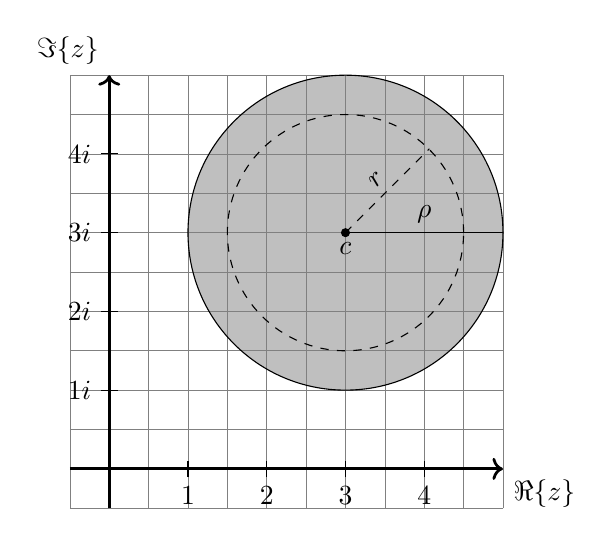
\begin{tikzpicture}
   % coords
   \coordinate (OR) at (0, 0);
   \coordinate (LX) at (-0.5, 0);
   \coordinate (RX) at (5, 0);
   \coordinate (TY) at (0, 5);
   \coordinate (BY) at (0, -0.5);

   % debugging grid
   \coordinate (BL) at (-0.5, -0.5);
   \coordinate (TR) at (5, 5);
   \draw[step=0.5cm, gray, very thin] (BL) grid (TR);

   % coordinate system
   \draw[->][line width=1.00pt] (LX) -- (RX) node[anchor=north west] {\(\Re\{z\}\)};
   \draw[->][line width=1.00pt] (BY) -- (TY) node[anchor=south east] {\(\Im\{z\}\)};
   \foreach \n in {1,2,...,4}{%
      \draw (\n,-3pt) node [below] {$\n$} -- (\n,3pt);
      \draw (-3pt,\n) node [left] {$\n i$} -- (3pt,\n);
   }

   \coordinate (c) at (3,3);
   \path[fill=gray, semitransparent] (c) circle (2);
   \draw[fill] (c) node[anchor=north]{\(c\)} circle [radius=0.05];
   \draw (c) circle (2);
   \draw (c) -- (5,3) node [midway, above, sloped, black] (TextNode) {\(\rho\)};

   \draw[dashed] (c) circle (1.5);
   \draw[dashed] (c) -- (4.065, 4.065) node [midway, above, sloped, black] (TextNode) {\(r\)};
\end{tikzpicture}

% \end{center}

\begin{theorem}[Power Series Convergence]\label{thm:conv_radius}
   Let \(\rho\) be the radius of convergence for \(\sum a_n z^n\).
   \[\forall z \in \mathbb{C}: \lvert z\rvert < \rho \implies \sum a_n z^n~\text{absolute convergent}\]
   \[\forall z \in \mathbb{C}: \lvert z\rvert > \rho \implies \sum a_n z^n~\text{divergent}\]
\end{theorem}
\begin{remark}
   For \(\lvert z\rvert = \rho\) we have to check for convergence seperately, i.e. we have to check if the series converges for \(z = \rho\) and \(z = -\rho\).
\end{remark}
\begin{example}
   For \(a_n := 1 \implies \sum_{n=0}^\infty z^n\) is \(\rho = 1\).
   The series converges to 0 for all \(|z| < 1\) and diverges for \(|z| \geq 1\).
\end{example}
\begin{example}
   For \(a_n := \frac{1}{n} \implies \sum_{n=0}^\infty \frac{1}{n} z^n\) is \(\rho = 1\).
   The series converges for \(|z| < 1\) and diverges for \(z = 1\).
   For \(z = -1\) is it the alternating harmonic series and converges.
\end{example}

\begin{proposition}[Important Power Series]
   The following are important examples of power series
   \begin{enumerate}[label=\roman*, align=Center]
      \item \(\forall z \in \mathbb{C}\)
         \[\sum_{n=0}^\infty \frac{1}{n!} z^n~\text{is absolute convergent}\]
      \item \(\forall z \in \mathbb{C}: \lvert z\rvert < 1\)
         \[\sum_{n=0}^\infty z^n~\text{is absolute convergent}\]
      \item Let \(z = 0\)
         \[\sum_{n=0}^\infty n! \cdot z^n~\text{is convergent}\]
      \item Let \(m \in \mathbb{Z}\) and \(\lvert z\rvert < 1\)
         \[\sum_{n=0}^\infty n^m \cdot z^n~\text{is convergent}\]
   \end{enumerate}
\end{proposition}

\begin{proposition}\label{pro:conv_rad_ratio_test}
   Let \(\rho\) be the radius of convergence of \(\sum a_n z^n\).
   \[\rho = \lim_{n \to \infty} \frac{\lvert a_n\rvert}{\lvert a_{n+1}\rvert}\]
\end{proposition}
\begin{remark}
   This proposition states that \(\rho\) can be calculated with the ratio test (\ref{pro:ratio_test}).
\end{remark}

\begin{theorem}
   Let \(\alpha \in \mathbb{C}\), \(\sum a_n z^n\) and \(\sum b_n z^n\) with radius of convergence \(\rho_a\) respectively \(\rho_b\).
   \begin{enumerate}[label=\roman*, align=Center]
      \item \(\forall z \in \mathbb{C}: \lvert z\rvert < \rho_a\)
         \[\sum \alpha \cdot a_n z^n = \alpha \cdot \sum a_n z^n\]
      \item \(\forall z \in \mathbb{C}: \lvert z\rvert < \min\{\rho_a, \rho_b\}\)
         \[\sum a_n z^n + \sum b_n z^n = \sum (a_n + b_n)z^n\]
      \item \(\forall \lvert z\rvert < \min\{\rho_a, \rho_b\}:\)
         \[\sum a_n z^n \cdot \sum b_n z^n = \sum_{n=0}^\infty\left(\sum_{k=0}^\infty a_k \cdot b_{n-k}\right)z^n\]
   \end{enumerate}
\end{theorem}

\subsection{Elementary Functions}
An \emph{elementary function} is a function of a single variable composed of particular simple functions.
They are typically defined as a sum, product, and/or composition of finitely many polynomials, rational functions, trigonometric and exponential functions, and their inverse functions.

\subsubsection{Exponential Function}
\begin{definition}[Exponential Function]
   Given \(z \in \mathbb{Z}\) we define \(\exp: \mathbb{C} \to \mathbb{C}\) by
   \[\exp(z) := \sum_{n = 0}^\infty \frac{z^n}{n!}\]
\end{definition}

\begin{proposition}[Properties]
   Let \(x, y, z \in \mathbb{C}\)
   \begin{enumerate}[label=\roman*, align=Center]
      \item The series has radius of convergence \(\rho = \infty\)
      \item \(\exp\) is continuous
      \item \(\exp(\alpha z) = \exp(z)^\alpha\)
      \item \(\exp(x + y) = \exp(x) \cdot \exp(y)\)
      \item \(\exp(-z) = \frac{1}{\exp(z)}\)
   \end{enumerate}
\end{proposition}

\begin{definition}[Eulers Number]
   \[e := \exp(1) = \sum_{n=0}^\infty \frac{1}{n!}\]
\end{definition}
\begin{remark}[Notation]
   From above we have \(e^z := \exp(z)\).
\end{remark}

Let \(z \in \mathbb{C}\), from above we see that
\[\exp(z) = \exp(x + iy) = \exp(x) \cdot \exp(iy)\]
which means that the complex \(\exp\) function is characterized by two parts
\[\exp: \mathbb{R} \to \mathbb{R} \qquad\text{and}\qquad \exp: i\mathbb{R} \to \mathbb{R}\]
We define the \emph{imaginary exponential function} \(\ixp: \mathbb{R} \to \mathbb{R}\) through \(\ixp(x) := \exp(ix)\).

\subsubsection{Logarithm}
\begin{proposition}
   We regard \(\exp: \mathbb{R} \to \mathbb{R}\), then
   \begin{enumerate}[label=\roman*, align=Center]
      \item \(\exp\) is strictly increasing
      \item \(\im(\exp) = \mathbb{R}_{>0}\)
      \item \(\forall n \in \mathbb{N}: \lim_{x \to \infty} \frac{\exp(x)}{x^n} = \infty\)
      \item \(\lim_{x \to -\infty} \exp(x) = 0\)
   \end{enumerate}
\end{proposition}
\begin{remark}[Intuition]
   We would split (ii) into the following observations:
   \[\forall x < 0: \exp(x) \in (0; 1) \qquad \forall x > 0: \exp(x) \in (1; \infty) \qquad \exp(0) = 1\]
   Point (iii) means that \(\exp\) grows faster than any other power.
\end{remark}

\begin{definition}[Logarithm]
   The inverse of \(\exp: \mathbb{R} \to \mathbb{R}_{>0}\) is
   \[\ln(x): \mathbb{R}_{>0} \to \mathbb{R} \qquad\text{where}\qquad \ln(x) = y \iff \exp(y) = x\]
\end{definition}

\begin{proposition}[Properties]
   Let \(x, y \in (0; \infty)\)
   \begin{enumerate}[label=\roman*, align=Center]
      \item \(\ln\) is continuous
      \item \(\ln\) is strictly increasing
      \item \(\lim_{x \to \infty} \ln(x) = \infty\)
      \item \(\lim_{x \to 0} \ln(x) = -\infty\)
      \item \(\ln(x^\alpha) = \alpha \cdot \ln(x)\)
      \item \(\ln(x \cdot y) = \ln(x) + \ln(y)\)
      \item \(\ln\left(\frac{x}{y}\right) = \ln(x) - \ln(y)\)
   \end{enumerate}
\end{proposition}
\begin{remark}
   From above we also have that \(\ln(1) = 0\).
\end{remark}

\subsubsection{Real Exponents}
Now that we have that \(x = \exp\big(\ln(x)\big)\) we can define \(x^r\) with \(r \in \mathbb{R}\).
First we need to check if everything remains the same as with whole exponents, so let \(n \in \mathbb{N}\) and \(x > 0\), then
\[x^n = \Big(\exp\big(\ln(x)\big)\Big)^n = \left(e^{\ln(x)}\right)^n = \exp\big(n \cdot \ln(x)\big)\]
\[x^{-n} = \frac{1}{x^n} = \frac{1}{\exp\big(n \cdot \ln(x)\big)} = \frac{1}{e^{n \cdot \ln(x)}} = e^{-n \cdot \ln(x)} = \exp\big(-n \cdot \ln(x)\big)\]
\[\sqrt[n]{x} = x^{\frac{1}{n}} = \Big(\exp\big(\ln(x)\big)\Big)^\frac{1}{n} = \exp\left(\frac{1}{n} \ln(x)\right)\]
and for \(p \in \mathbb{Z}\), \(q \in \mathbb{N}_{>0}\)
\[x^\frac{p}{q} = \Big(\exp\big(\ln(x)\big)\Big)^\frac{p}{q} = \exp\left(\frac{p}{q} \ln(x)\right)\]

\begin{definition}[Real Exponents]\label{def:real_exponents}
   Given \(x > 0\) and \(r \in \mathbb{R}\)
   \[x^r := \exp\big(r \cdot \ln(x)\big)\]
\end{definition}

\begin{proposition}[Calculation Rules]
   Let \(x, y \in \mathbb{R}_{>0}\) and \(r, s \in \mathbb{R}\), then
   \begin{enumerate}[label=\roman*, align=Center]
      \item \(x^r \cdot x^s = x^{r + s}\)
      \item \(\frac{x^r}{x^s} = x^{r-s}\)
      \item \(x^r \cdot y^r = (x \cdot y)^r\)
      \item \((x^r)^s = x^{r \cdot s}\)
      \item \(\ln(x^r) = r \cdot \ln(x)\)
   \end{enumerate}
\end{proposition}

\begin{proposition}
   Let \(r \in \mathbb{R}_{>0}\) then
   \[\lim_{x \to \infty} \left(x^{-r} \cdot \ln(x)\right) = 0 \qquad\text{and}\qquad \lim_{x \to 0} \left(x^r \cdot \ln(x)\right) = 0\]
\end{proposition}
\begin{remark}
   This proposition states that \(\ln\) is damped by \(\frac{1}{x^n}\).
\end{remark}

\subsubsection{Trigonometric Functions}
\begin{definition}[Cosine]
   Given \(z \in \mathbb{C}\) we define \(\cos: \mathbb{C} \to \mathbb{C}\) by
   \[\cos(z) := \sum_{n=0}^\infty (-1)^n \frac{z^{2n}}{(2n)!}\]
\end{definition}

\begin{definition}[Sine]
   Given \(z \in \mathbb{C}\) we define \(\sin: \mathbb{C} \to \mathbb{C}\) by
   \[\sin(z) := \sum_{n=0}^\infty (-1)^n \frac{z^{2n + 1}}{(2n+1)!}\]
\end{definition}

\begin{proposition}[Properties]
   Let \(z, w \in \mathbb{C}\), then
   \begin{enumerate}[label=\roman*, align=Center]
      \item Both series have radius of convergence \(\rho = \infty\)
      \item \(\cos\) and \(\sin\) are continuous
      \item \(\cos(-z) = \cos(z)\)
      \item \(\sin(-z) = -\sin(z)\)
      \item \(\cos(z \pm w) = \cos(z) \cdot \cos(w) \mp \sin(z) \cdot \sin(w)\)
      \item \(\sin(z \pm w) = \sin(z) \cdot \cos(w) \pm \cos(z) \cdot \sin(w)\)
      \item \(\sin(z) - \sin(w) = 2 \cos\left(\frac{z+w}{2}\right) \cdot \sin\left(\frac{z-w}{2}\right)\)
      \item \(\cos(z) - \cos(w) = -2 \sin\left(\frac{z+w}{2}\right) \cdot \sin\left(\frac{z-w}{2}\right)\)
      \item \(\cos^2(z) + \sin^2(z) = 1\)
   \end{enumerate}
\end{proposition}

\subsubsection{Connecting Exponential and Trigonometric}
Recall that \(\ixp(x) := \exp(ix)\).

\begin{proposition}
   Let \(x \in \mathbb{R}\) and \(z \in \mathbb{C}\), then
   \begin{enumerate}[label=\roman*, align=Center]
      \item \(\cos(x) = \Re\big(\exp(ix)\big)\)
      \item \(\sin(x) = \Im\big(\exp(ix)\big)\)
      \item \(\exp(ix) = \cos(x) + i \cdot \sin(x)\)
      \item \[\cos(z) = \frac{\exp(iz) + \exp(-iz)}{2}\]
      \item \[\sin(z) = \frac{\exp(iz) - \exp(-iz)}{2i}\]
   \end{enumerate}
\end{proposition}

\begin{theorem}[Unit Circle]
   \(\im(\ixp) = S^1 := \{z \in \mathbb{C} \mid \lvert z\rvert = 1\}\)
\end{theorem}
\begin{center}
   \begin{tikzpicture}[line cap=round,line join=round,>=triangle 45,x=1cm,y=1cm]
   \begin{axis}[
   x=5cm,y=5cm,
   axis lines=middle,
   ymajorgrids=true,
   xmajorgrids=true,
   xmin=-1.1, xmax=1.1,
   ymin=-1.1, ymax=1.1,
   xtick={-1,-0.8,...,1},
   ytick={-1,-0.8,...,1},]

   \draw [line width=2pt,color=black] (0,0) circle (5cm);

   \draw [line width=2pt, color=black] (0,0)-- (0.6,0.8);

   \draw [line width=1pt, dashed]  (0.6,0)-- (0.6,0.8);
   \draw [line width=1pt, dashed] (0,0.8)-- (0.6,0.8);

   \draw [line width=2pt,color=red] (0,0)-- (0.6,0);
   \draw [line width=2pt,color=blue] (0,0)-- (0,0.8);

   \draw [fill=grey] (0.6,0.8) circle (2.5pt);
   \draw (0.67, 0.87 ) node {\(e^{it}\)};
   \draw (-0.6, 1) node {\(\{z \in \mathbb{C} \mid |z| = 1\}\)};

   \draw (0.3, 0.05) node {\(\cos(t)\)};
   \draw (0.12, 0.4) node {\(\sin(t)\)};
   \end{axis}
\end{tikzpicture}

\end{center}

\begin{theorem}
   The set
   \[M := \{x \in (0; \infty) \mid \ixp(x) = 1\}\]
   has a positive minimum
   \[\pi := \frac{1}{2} \min(M)\]
\end{theorem}

\begin{definition}[Periodic Function]
   \(f: \mathbb{K} \to \mathbb{K}\) is \(p\)-periodic iff
   \[\forall x \in \mathbb{K}: f(x + p) = f(x)\]
\end{definition}

\begin{theorem}
   Let \(z \in \mathbb{C}\) and \(k \in \mathbb{Z}\), then
   \[\exp(z) = 1 \iff z = 2 \pi i \cdot k\]
   \[\exp(z) = -1 \iff z = (2k + 1)\pi i\]
\end{theorem}
\begin{remark}
   It follows that for \(k \in \mathbb{Z}\) holds \(\exp(z) = \exp(z + 2k\pi i)\) i.e. \(\exp\) is \(2\pi i\)-periodic.
\end{remark}

\begin{theorem}
   For \(x \in \mathbb{R}\) is \(\ixp: [x; x + 2\pi) \to S^1\) bijective.
\end{theorem}

\begin{proposition}[Properties]
   Let \(k \in \mathbb{Z}\) and \(z \in \mathbb{C}\), then
   \begin{enumerate}[label=\roman*, align=Center]
      \item \(\cos(z) = \cos(z + 2k\pi)\)
      \item \(\cos(k\pi) = (-1)^k\)
      \item \(\sin(z) = \sin(z + 2k\pi)\)
      \item \(\sin\left((2k+1)\frac{\pi}{2}\right) = (-1)^k\)
      \item \(\cos(z) = 0 \iff z = \frac{\pi}{2} + k\pi\)
      \item \(\sin(z) = 0 \iff z = k\pi\)
      \item \(\forall x \in (0; \pi): \sin(x) > 0\)
      \item \(\forall x \in \left(0; \frac{\pi}{2}\right): \cos(x) > 0\)
      \item \(\sin\) is strictly increasing on \(\left[0; \frac{\pi}{2}\right]\)
      \item \(\sin(z + \pi) = -\sin(z)\)
      \item \(\cos(z + \pi) = -\cos(z)\)
      \item \(\sin\left(\frac{\pi}{2} - z\right) = \cos(z)\)
      \item \(\cos\left(\frac{\pi}{2} - z\right) = \sin(z)\)
      \item \(\im(\cos) = \im(\sin) = [-1;1]\)
   \end{enumerate}
\end{proposition}
\begin{remark}
   The following table displays common values of the trigonometric functions.
   \begin{center}
      \renewcommand\arraystretch{1.3}
      \begin{tabular}{c|c|c|c|c|c}
              & \(0^\circ\) & \(30^\circ\) & \(45^\circ\) & \(60^\circ\) & \(90^\circ = \frac{\pi}{2}\)\\
         \hline
         \(\sin\) & \(\frac{\sqrt{0}}{2}\) & \(\frac{\sqrt{1}}{2}\) & \(\frac{\sqrt{2}}{2}\) & \(\frac{\sqrt{3}}{2}\) & \(\frac{\sqrt{4}}{2}\)\\
         \hline
         \(\cos\) & \(\frac{\sqrt{4}}{2}\) & \(\frac{\sqrt{3}}{2}\) & \(\frac{\sqrt{2}}{2}\) & \(\frac{\sqrt{1}}{2}\) & \(\frac{\sqrt{0}}{2}\)\\
      \end{tabular}
   \end{center}
\end{remark}

\begin{theorem}
   For \(x \in \mathbb{R}\) is \(\exp: \mathbb{R} + i[x; x + 2\pi) \to \mathbb{C}\setminus\{0\}\) bijective.
\end{theorem}

\begin{theorem}[Polar Coordinates]
   For any \(z \in \mathbb{C}\setminus\{0\}\),
   \[\exists! \theta \in [0; 2\pi): z = \lvert z\rvert \cdot \exp(i \theta)\]
\end{theorem}
We call \(\theta\) the \emph{argument} of \(z\), denoted \(\argu(z) := \theta\).
With this we can derive \emph{polar coordinates} of any complex number \(z\)
\[z = x + iy = r \cdot \exp(i \theta) \qquad\text{where}~r := |z| = \sqrt{x^2 + y^2}\]
The values \(x\) and \(y\) are called the \emph{Cartesian coordinates} of \(z\), while \(r\) and \(\theta\) are its \emph{polar coordinates}.
Now note that
\[z = x + iy = \lvert z\rvert \cdot \exp(i \theta) = \lvert z \rvert \cdot \big(\cos(\theta) + i\sin(\theta)\big) = \lvert z\rvert\cos(\theta) + i\lvert z\rvert\sin(\theta)\]
hence we have
\[\cos(\theta) = \frac{\Re(z)}{\lvert z\rvert} \qquad\text{and}\qquad \sin(\theta) = \frac{\Im(z)}{\lvert z\rvert}\]
\begin{example}
   Let \(z := -\sqrt{3} + i3\), we compute its polar coordinates.

   First we compute \(\lvert z\rvert = \sqrt{(-\sqrt{3})^2 + 3^2} = \sqrt{12}\).
   Then we solve
   hence
   \[-\sqrt{3} + i3 = \sqrt{12}\cos(\theta) + i\sqrt{12}\sin(\theta) \implies \begin{cases}
         -\sqrt{3} = \sqrt{12}\cos(\theta) \implies \cos(\theta) = -\frac{\sqrt{3}}{\sqrt{12}} = -\frac{1}{2}\\
         3 = \sqrt{12}\sin(\theta) \implies \sin(\theta) = \frac{3}{\sqrt{12}} = \frac{\sqrt{3}}{2}
   \end{cases}\]
   Now we lookup the values on the unit circle and get that \(\theta = \frac{2\pi}{3}\).
\end{example}

% TODO: make better drawing
% \begin{center}
%    \begin{tikzpicture}[line cap=round,line join=round,>=triangle 45,x=1cm,y=1cm]
   \begin{axis}[
   x=1cm,y=1cm,
   axis lines=middle,
   ymajorgrids=true,
   xmajorgrids=true,
   xmin=-3.6423644972783227,
   xmax=9.836484290540891,
   ymin=-2.466863579845977,
   ymax=5.846571116588563,
   xtick={-3,-2,...,9},
   ytick={-2,-1,...,5},]
      \draw [shift={(0,0)},line width=2pt,fill=black,fill opacity=0.10000000149011612] (0,0) -- (0:0.33253738785738196) arc (0:30.96375653207352:0.33253738785738196) -- cycle;
      \draw [line width=1.2pt,dashed] (5,3)-- (5,0);
      \draw [line width=1.2pt,dashed] (5,3)-- (0,3);
      \draw [line width=2pt,color=grey] (0,0)-- (5,3);
      \draw [line width=2pt,color=blue] (0,0)-- (0,3);
      \draw [line width=2pt,color=red] (0,0)-- (5,0);
      \draw [fill=blue] (5,3) circle (2.5pt);
      \draw[color=blue] (6.466772093586088,3.236152621908117) node {\(z = x + iy = |z| * \exp(i\theta)\)};
      \draw[color=grey] (2.7201841903929185,1.4847890458592405) node {|z|};
      \draw[color=black] (0.6695369652723964,0.1878932332154525) node {\(\theta\)};
      \draw[color=blue] (-0.18397566356155054,1.5956348418117012) node {\(iy\)};
      \draw[color=red] (2.5428309168689816,-0.044882938284714596) node {\(x\)};
   \end{axis}
\end{tikzpicture}

% \end{center}

\begin{theorem}[Complex nth-Root]
   For \(x \in \mathbb{C}\) has \(z^n = x\) \(n\) distinct solutions
   \[z_k = \lvert x\rvert^\frac{1}{n} \exp\left(\frac{i(\argu(x) + 2\pi k)}{n}\right)\]
\end{theorem}
\begin{example}
   We want to find the 6th roots of \(x := 4 + i4\sqrt{3}\).

   So first we compute
   \[\lvert x\rvert = \sqrt{4^2 +4^2\cdot 3} = \sqrt{64} = 8 \rightsquigarrow \cos(\theta)=\frac{4}{8} = \frac{1}{2} \quad \sin(\theta) = \frac{4\sqrt{3}}{8} = \frac{\sqrt{3}}{2}\]
   where we get \(\theta = \frac{\pi}{3} = \argu(x)\)
   So we can compute our 6 solutions with the theorem above
   \[z_k = \sqrt[6]{8} \cdot \exp\left(\frac{i(\frac{\pi}{3} + 2\pi k)}{6}\right) = \sqrt[6]{8} \left(\cos\left(\frac{\pi}{18} + \frac{\pi}{3} k\right) + i \sin\left(\frac{\pi}{18} + \frac{\pi}{3}k\right)\right)\]
   hence we get
   \[z_0 = \sqrt[6]{8}\left(\cos\left(\frac{\pi}{18}\right) + i\sin\left(\frac{\pi}{18}\right)\right)\]
   \[z_1 = \sqrt[6]{8}\left(\cos\left(\frac{7\pi}{18}\right) + i\sin\left(\frac{7\pi}{18}\right)\right)\]
   \[z_2 = \sqrt[6]{8}\left(\cos\left(\frac{13\pi}{18}\right) + i\sin\left(\frac{13\pi}{18}\right)\right)\]
   \[z_3 = \sqrt[6]{8}\left(\cos\left(\frac{19\pi}{18}\right) + i\sin\left(\frac{19\pi}{18}\right)\right)\]
   \[z_4 = \sqrt[6]{8}\left(\cos\left(\frac{25\pi}{18}\right) + i\sin\left(\frac{25\pi}{18}\right)\right)\]
   \[z_5 = \sqrt[6]{8}\left(\cos\left(\frac{31\pi}{18}\right) + i\sin\left(\frac{31\pi}{18}\right)\right)\]
\end{example}

\newpage

\section{Continuity}
A rigorous definition of continuity of real functions is usually given in terms of the idea of a limit of those functions.
So far we only looked at limits of sequences, so now we want to regard the limit of functions.

\subsection{Function Limits}\label{ssec:function_limits}
\begin{definition}[Function Limit]\label{def:func_limit}
   Given \(f: D \to \mathbb{R}\) and \(x_0 \in D\),
   \[\lim_{x \to x_0}\big(f(x)\big) = L :\iff \forall \varepsilon > 0~\exists \delta > 0: (\forall x \in D: \lvert x - x_0 \rvert < \delta \implies \lvert f(x) - L\rvert < \varepsilon\]
\end{definition}
\begin{remark}[Intuition]
   Note that we can rewrite the condition above as
   \[\forall x \in (x_0 - \delta; x_0 + \delta): f(x) \in \big(L - \varepsilon; L + \varepsilon\big)\]
   \begin{center}
      \begin{tikzpicture}[line cap=round,line join=round,>=triangle 45,x=1cm,y=1cm]
   \begin{axis}[
   ticks=none,
   x=2cm, y=2cm,
   axis lines=middle,
   ymajorgrids=true,
   xmajorgrids=true,
   xmin=-0.4, xmax=6.1,
   ymin=-0.4, ymax=3.1]
      \fill[line width=2pt,color=gray,fill=gray,fill opacity=0.1] (0,2.2) -- (8,2.2) -- (8,1) -- (0,1) -- cycle;
      \draw[line width=2pt,color=blue,smooth,samples=100,domain=-0.3:7] plot(\x,{ln((\x)+1)});

      \draw [line width=1pt,dashed] (0,1.6079667094364514) -- (4.000000075430033,1.6094379275201067);
      \draw [line width=1pt,dashed] (4.000000075430033,1.6094379275201067)-- (4,0);
      \draw [line width=1pt] (3,0) -- (2.9996517855796725,1.3862073037254237);
      \draw [line width=1pt] (5,0) -- (5.000842962216623,1.7918999530625097);
      \draw [line width=1pt] (0,2.2) -- (8,2.2);
      \draw [line width=1pt] (8,1) -- (0,1);

      \draw [line width=4pt,color=orange] (2.9996517855796725,1.3862073037254237)-- (3.199034292788041,1.4348545685627394)-- (3.399609048748734,1.4815156844194872)-- (3.5985123484097543,1.5257328486695583)-- (3.799087104370447,1.5684257132365922)-- (4.000000075430033,1.6094379275201067)-- (4.200236616291833,1.6487041276851904)-- (4.402482828552198,1.6868586309676052)-- (4.6013861282132185,1.7230140900075834)-- (4.8002894278742385,1.7579078176649696)-- (5.000842962216623,1.7918999530625097);

      \draw [fill=blue] (0,2.2) circle (2.5pt);
      \draw (0.39, 2.33) node {\(L + \varepsilon\)};
      \draw [fill=blue] (0,1.6079667094364514) circle (2.5pt);
      \draw (0.29, 1.7408231122516713) node {\(L\)};
      \draw [fill=blue] (0,1) circle (2.5pt);
      \draw (0.39, 1.13) node {\(L - \varepsilon\)};

      \draw [fill=blue] (4.000000075430033,1.6094379275201067) circle (2.5pt);

      \draw [fill=blue] (5,0) circle (2.5pt);
      \draw (5, -0.15) node {\(x_0 + \delta\)};
      \draw [fill=blue] (4,0) circle (2.5pt);
      \draw (4, -0.15) node {\(x_0\)};
      \draw [fill=blue] (3,0) circle (2.5pt);
      \draw (3, -0.15) node {\(x_0 - \delta\)};
   \end{axis}
\end{tikzpicture}

   \end{center}
\end{remark}
Now we see that the concept of the limit of a function is connected to the concept of the limit of sequences.
\begin{proposition}[Function Limit = Sequence Limit]
   Let \(f: D \to \mathbb{R}\) and \(x_0 \in X\),
   \[\lim_{x \to x_0}\big(f(x)\big) = L \iff \forall x_n \in \big(D\setminus\{x_0\}\big)^\mathbb{N}: \left(\lim_{n \to \infty}(x_n) = x_0 \implies  \lim_{n \to \infty}\big(f(x_n)\big) = L\right)\]
\end{proposition}
\begin{remark}[Intuition]
   We regard all sequences \(x_n\) in the domain of \(f\) which converge to the input \(x_0\).
   Then we take each sequence, use it as inputs for \(f\) and create a sequence of function values.
   If all those sequences of function values converge to \(L\), we say \(L\) is the limit of \(f\) as \(x \to x_0\).
\end{remark}

\subsubsection{Computing Function Limits}
As the limit of sequences and functions are equivalent we can derive calculation rules for function limits from \cref{pro:seq_limit_rules}.
\begin{proposition}[Function Limit Rules]
   Let \(f: I \to \mathbb{R}\), \(g: I \to \mathbb{R}\) and \(c \in \mathbb{R}\), then

   \begin{enumerate}[label=\roman*, align=Center]
      \item \[\lim_{x \to x_0}\big(f(x) \pm g(x)\big) = \lim_{x \to x_0}\big(f(x)\big) \pm \lim_{x \to x_0}\big(g(x)\big)\]
      \item \[\lim_{x \to x_0}\big(c \cdot f(x)\big) = c \cdot \lim_{x \to x_0}\big(f(x)\big)\]
      \item \[\lim_{x \to x_0}\big(f(x) \cdot g(x)\big) = \lim_{x \to x_0}\big(f(x)\big) \cdot \lim_{x \to x_0}\big(g(x)\big)\]
      \item \[\lim_{x \to x_0}\left(\frac{f(x)}{g(x)}\right) = \frac{\lim_{x \to x_0}\big(f(x)\big)}{\lim_{x \to x_0}\big(g(x)\big)}\]
   \end{enumerate}
\end{proposition}

\paragraph{The Root-Trick} is a usefull method to determine limits which contain \(\sqrt{x}\).
\begin{example}
   We want to find \(\lim_{x \to \infty}\big(f(x)\big)\) where \(f(x) := \sqrt{x^2 + x} - x\).
\begin{equation*}
   \begin{split}
      \lim_{x \to \infty} \left(\sqrt{x^2 + x} - x\right) & = \lim_{x \to \infty} \left(\left(\sqrt{x^2 + x} - x\right) \frac{\left(\sqrt{x^2 + x} + x\right)}{\left(\sqrt{x^2 + x} + x\right)}\right) = \lim_{x \to \infty} \left(\frac{x^2 + x - x^2}{\sqrt{x^2 + x} + x}\right) =\\
                                                          & = \lim_{x \to \infty} \left(\frac{x}{\sqrt{x^2 + x} + x}\right) = \lim_{x \to \infty}\left(\frac{x}{x \left(\frac{\sqrt{x^2 + x}}{x} + 1\right)}\right) = \frac{1}{\lim_{x \to \infty}\left(\frac{\sqrt{x^2 + x}}{x} + 1\right)} =\\
                                                          & = \frac{1}{\lim_{x \to \infty}\left(\sqrt{\frac{x^2 + x}{x^2}}\right) + 1} = \frac{1}{\sqrt{\lim_{x \to \infty}\left(\frac{x^2 \left(1 + \frac{1}{x}\right)}{x^2}\right)} + 1} = \frac{1}{\sqrt{\lim_{x \to \infty}\left(1 + \frac{1}{x}\right)} + 1} =\\
                                                          & = \frac{1}{\sqrt{1} + 1} = \frac{1}{2}
   \end{split}
\end{equation*}
\end{example}

\paragraph{The Fundamental Limit \(e\)} is given by
\[\lim_{x \to \infty} \left(1 + \frac{1}{x}\right)^x = e \qquad\text{and}\qquad \lim_{x \to 0} (1 + x)^{\frac{1}{x}} = e\]
From this follows (not trivially) a neat trick:
\[\lim_{x \to x_0} \left(1 + \frac{1}{\ast}\right)^* = e\]
where \(\ast\) is some term in \(x\) with \(\ast \xrightarrow{x \to x_0} \infty\).
Equivalently we have
\[\lim_{x \to x_0} (1 + \ast)^{\frac{1}{\ast}} = e\]
where \(\ast \xrightarrow{x \to x_0} 0\).
\begin{example}
   We want to find \(\lim_{x \to \infty}\big(f(x)\big)\) where \(f(x) := \left(1 - \frac{3}{x}\right)^{2x}\).
   \[\lim_{x \to \infty} \left(1 - \frac{3}{x}\right)^{2x} = \lim_{x \to \infty} \left(\left(1 + \frac{1}{-\frac{x}{3}}\right)^{-\frac{x}{3}}\right)^{-\frac{3}{x} \cdot 2x} = \lim_{x \to \infty}\Big(e^{-\frac{6x}{x}}\Big) = e^{-6}\]
\end{example}

\paragraph{The Fundamental Limit \(\sin(x)\)} is given by
\[\lim_{x \to 0}\left(\frac{\sin(x)}{x}\right) = 1\]
From this follows a neat trick:
\[\lim_{x \to x_0} \frac{\sin(\ast)}{\ast} = 1\]
where \(\ast\) is some term in \(x\) with \(\ast \xrightarrow{x \to x_0} 0\).
\begin{example}
   We want to find \(\lim_{x \to 1} \frac{\sin(1-x^2)}{1-x}\)
   \[\lim_{x \to 1} \frac{\sin(1-x^2)}{1-x} = \lim_{x \to 1}\frac{\sin(1-x^2)}{1-x^2} \cdot \frac{1-x^2}{1-x} = 1 \cdot \lim_{x \to 1} \frac{(1-x)(1+x)}{1-x} = \lim_{x \to 1} 1 + x = 2\]
\end{example}

\paragraph{The \(e^{\log}\) - Trick} derived from \cref{def:real_exponents}, is a usefull method to determine limits \(\lim_{x \to x_0} f(x)^{g(x)}\).
The main idea is to rewrite
\[f(x)^{g(x)} = \exp\Big(\log\big(f(x)^{g(x)}\big)\Big) = \exp\Big(g(x) \cdot \log\big(f(x)\big)\Big)\]
as \(\exp\) is continuous, we can pull the limit into the argument.
\begin{equation*}
   \begin{split}
      \lim_{x \to x_0} f(x)^{g(x)} &= \lim_{x \to x_0} e^{\log(f(x)^{g(x)})} = \lim_{x \to x_0} e^{g(x) \cdot \log(f(x))} \overset{e~\text{cont.}}{=} \exp\left(\lim_{x \to x_0} \Big(g(x) \cdot log\big(f(x)\big)\Big)\right) = \\
                                   & = \exp\left(\lim_{x \to x_0}g(x) \cdot \lim_{x \to x_0}\Big(\log\big(f(x)\big)\Big)\right) \overset{\ln~\text{cont.}}{=} \exp\left(\lim_{x \to x_0}g(x) \cdot \log\left(\lim_{x \to x_0}f(x)\right)\right)
   \end{split}
\end{equation*}
% TODO
\begin{example}
\end{example}

\subsubsection{One-Sided Limits}
Another intuitive viewpoint to see how function limits and continuity are connected is the following.
\begin{definition}[One-Sided Limit]\label{def:one-sided_limit}
   Given \(x_0 \in \overline{\mathbb{R}}\) and \(f: [a;b] \to \mathbb{R}\),
   \[\lim_{x \uparrow x_0}\big(f(x)\big) := \lim_{x \to x_0}\big(f|_{D \cap (-\infty; x_0)}\big)\]
   \[\lim_{x \downarrow x_0}\big(f(x)\big) := \lim_{x \to x_0}\big(f|_{D \cap (x_0; \infty)}\big)\]
\end{definition}
\begin{remark}[Terminology]
   We call \(\lim_{x \uparrow x_0} f(x)\) a \emph{left-handed} and \(\lim_{x \downarrow x_0} f(x)\) a \emph{right-handed} limit.
\end{remark}
\begin{remark}[Notation]
   There are many equivalent ways of denoting left- and right-handed limits
   \[\lim_{x \downarrow x_0}\big(f(x)\big) \qquad \lim_{x \to x_0^+}\big(f(x)\big) \qquad \lim_{x \searrow x_0}\big(f(x)\big)\]
   \[\lim_{x \uparrow x_0}\big(f(x)\big) \qquad \lim_{x \to x_0^-}\big(f(x)\big) \qquad \lim_{x \nearrow x_0}\big(f(x)\big)\]
\end{remark}
\begin{remark}
   From \cref{def:func_limit} we can equivalently write
   \[\lim_{x \uparrow x_0} f(x) = L \iff \forall \varepsilon~\exists \delta > 0: (x \in D: x_0- \delta < x < x_0 \implies |f(x) - L| < \varepsilon)\]
   \[\lim_{x \downarrow x_0} f(x) = L \iff \forall \varepsilon~\exists \delta > 0: (x \in D: x_0 < x < x_0 + \delta \implies |f(x) - L| < \varepsilon)\]
\end{remark}
\begin{example}
   We regard
   \[f(x) = \begin{cases}0 & x \leq 0\\ 1 & x > 0\end{cases}\]
   where we see that
   \[\lim_{x \uparrow 0} f(x) = 0 \qquad \lim_{x \downarrow 0} f(x) = 1\]
\end{example}
\begin{center}
   \begin{tikzpicture}[line cap=round,line join=round,>=triangle 45,x=1cm,y=1cm]
   \begin{axis}[
   x=4cm,y=4cm,
   axis lines=middle,
   ymajorgrids=true,
   xmajorgrids=true,
   xmin=-0.7,
   xmax=0.7,
   ymin=-0.1,
   ymax=1.1,
   xtick={-1,0,1},
   ytick={-1,0,1},]
   \draw[line width=2pt,color=blue] (-1.2292426079511276,0) -- (-1.2292426079511276,0);
   \draw[line width=2pt,color=blue] (-1.2292426079511276,0) -- (-1.2226596040846602,0);
   \draw[line width=2pt,color=blue] (-1.2226596040846602,0) -- (-1.2160766002181929,0);
   \draw[line width=2pt,color=blue] (-1.2160766002181929,0) -- (-1.2094935963517255,0);
   \draw[line width=2pt,color=blue] (-1.2094935963517255,0) -- (-1.2029105924852581,0);
   \draw[line width=2pt,color=blue] (-1.2029105924852581,0) -- (-1.1963275886187907,0);
   \draw[line width=2pt,color=blue] (-1.1963275886187907,0) -- (-1.1897445847523234,0);
   \draw[line width=2pt,color=blue] (-1.1897445847523234,0) -- (-1.183161580885856,0);
   \draw[line width=2pt,color=blue] (-1.183161580885856,0) -- (-1.1765785770193886,0);
   \draw[line width=2pt,color=blue] (-1.1765785770193886,0) -- (-1.1699955731529212,0);
   \draw[line width=2pt,color=blue] (-1.1699955731529212,0) -- (-1.1634125692864539,0);
   \draw[line width=2pt,color=blue] (-1.1634125692864539,0) -- (-1.1568295654199865,0);
   \draw[line width=2pt,color=blue] (-1.1568295654199865,0) -- (-1.1502465615535191,0);
   \draw[line width=2pt,color=blue] (-1.1502465615535191,0) -- (-1.1436635576870517,0);
   \draw[line width=2pt,color=blue] (-1.1436635576870517,0) -- (-1.1370805538205844,0);
   \draw[line width=2pt,color=blue] (-1.1370805538205844,0) -- (-1.130497549954117,0);
   \draw[line width=2pt,color=blue] (-1.130497549954117,0) -- (-1.1239145460876496,0);
   \draw[line width=2pt,color=blue] (-1.1239145460876496,0) -- (-1.1173315422211823,0);
   \draw[line width=2pt,color=blue] (-1.1173315422211823,0) -- (-1.1107485383547149,0);
   \draw[line width=2pt,color=blue] (-1.1107485383547149,0) -- (-1.1041655344882475,0);
   \draw[line width=2pt,color=blue] (-1.1041655344882475,0) -- (-1.0975825306217801,0);
   \draw[line width=2pt,color=blue] (-1.0975825306217801,0) -- (-1.0909995267553128,0);
   \draw[line width=2pt,color=blue] (-1.0909995267553128,0) -- (-1.0844165228888454,0);
   \draw[line width=2pt,color=blue] (-1.0844165228888454,0) -- (-1.077833519022378,0);
   \draw[line width=2pt,color=blue] (-1.077833519022378,0) -- (-1.0712505151559106,0);
   \draw[line width=2pt,color=blue] (-1.0712505151559106,0) -- (-1.0646675112894433,0);
   \draw[line width=2pt,color=blue] (-1.0646675112894433,0) -- (-1.0580845074229759,0);
   \draw[line width=2pt,color=blue] (-1.0580845074229759,0) -- (-1.0515015035565085,0);
   \draw[line width=2pt,color=blue] (-1.0515015035565085,0) -- (-1.0449184996900411,0);
   \draw[line width=2pt,color=blue] (-1.0449184996900411,0) -- (-1.0383354958235738,0);
   \draw[line width=2pt,color=blue] (-1.0383354958235738,0) -- (-1.0317524919571064,0);
   \draw[line width=2pt,color=blue] (-1.0317524919571064,0) -- (-1.025169488090639,0);
   \draw[line width=2pt,color=blue] (-1.025169488090639,0) -- (-1.0185864842241716,0);
   \draw[line width=2pt,color=blue] (-1.0185864842241716,0) -- (-1.0120034803577043,0);
   \draw[line width=2pt,color=blue] (-1.0120034803577043,0) -- (-1.005420476491237,0);
   \draw[line width=2pt,color=blue] (-1.005420476491237,0) -- (-0.9988374726247695,0);
   \draw[line width=2pt,color=blue] (-0.9988374726247695,0) -- (-0.9922544687583021,0);
   \draw[line width=2pt,color=blue] (-0.9922544687583021,0) -- (-0.9856714648918348,0);
   \draw[line width=2pt,color=blue] (-0.9856714648918348,0) -- (-0.9790884610253674,0);
   \draw[line width=2pt,color=blue] (-0.9790884610253674,0) -- (-0.9725054571589,0);
   \draw[line width=2pt,color=blue] (-0.9725054571589,0) -- (-0.9659224532924326,0);
   \draw[line width=2pt,color=blue] (-0.9659224532924326,0) -- (-0.9593394494259653,0);
   \draw[line width=2pt,color=blue] (-0.9593394494259653,0) -- (-0.9527564455594979,0);
   \draw[line width=2pt,color=blue] (-0.9527564455594979,0) -- (-0.9461734416930305,0);
   \draw[line width=2pt,color=blue] (-0.9461734416930305,0) -- (-0.9395904378265632,0);
   \draw[line width=2pt,color=blue] (-0.9395904378265632,0) -- (-0.9330074339600958,0);
   \draw[line width=2pt,color=blue] (-0.9330074339600958,0) -- (-0.9264244300936284,0);
   \draw[line width=2pt,color=blue] (-0.9264244300936284,0) -- (-0.919841426227161,0);
   \draw[line width=2pt,color=blue] (-0.919841426227161,0) -- (-0.9132584223606937,0);
   \draw[line width=2pt,color=blue] (-0.9132584223606937,0) -- (-0.9066754184942263,0);
   \draw[line width=2pt,color=blue] (-0.9066754184942263,0) -- (-0.9000924146277589,0);
   \draw[line width=2pt,color=blue] (-0.9000924146277589,0) -- (-0.8935094107612915,0);
   \draw[line width=2pt,color=blue] (-0.8935094107612915,0) -- (-0.8869264068948242,0);
   \draw[line width=2pt,color=blue] (-0.8869264068948242,0) -- (-0.8803434030283568,0);
   \draw[line width=2pt,color=blue] (-0.8803434030283568,0) -- (-0.8737603991618894,0);
   \draw[line width=2pt,color=blue] (-0.8737603991618894,0) -- (-0.867177395295422,0);
   \draw[line width=2pt,color=blue] (-0.867177395295422,0) -- (-0.8605943914289547,0);
   \draw[line width=2pt,color=blue] (-0.8605943914289547,0) -- (-0.8540113875624873,0);
   \draw[line width=2pt,color=blue] (-0.8540113875624873,0) -- (-0.8474283836960199,0);
   \draw[line width=2pt,color=blue] (-0.8474283836960199,0) -- (-0.8408453798295525,0);
   \draw[line width=2pt,color=blue] (-0.8408453798295525,0) -- (-0.8342623759630852,0);
   \draw[line width=2pt,color=blue] (-0.8342623759630852,0) -- (-0.8276793720966178,0);
   \draw[line width=2pt,color=blue] (-0.8276793720966178,0) -- (-0.8210963682301504,0);
   \draw[line width=2pt,color=blue] (-0.8210963682301504,0) -- (-0.814513364363683,0);
   \draw[line width=2pt,color=blue] (-0.814513364363683,0) -- (-0.8079303604972157,0);
   \draw[line width=2pt,color=blue] (-0.8079303604972157,0) -- (-0.8013473566307483,0);
   \draw[line width=2pt,color=blue] (-0.8013473566307483,0) -- (-0.7947643527642809,0);
   \draw[line width=2pt,color=blue] (-0.7947643527642809,0) -- (-0.7881813488978135,0);
   \draw[line width=2pt,color=blue] (-0.7881813488978135,0) -- (-0.7815983450313462,0);
   \draw[line width=2pt,color=blue] (-0.7815983450313462,0) -- (-0.7750153411648788,0);
   \draw[line width=2pt,color=blue] (-0.7750153411648788,0) -- (-0.7684323372984114,0);
   \draw[line width=2pt,color=blue] (-0.7684323372984114,0) -- (-0.761849333431944,0);
   \draw[line width=2pt,color=blue] (-0.761849333431944,0) -- (-0.7552663295654767,0);
   \draw[line width=2pt,color=blue] (-0.7552663295654767,0) -- (-0.7486833256990093,0);
   \draw[line width=2pt,color=blue] (-0.7486833256990093,0) -- (-0.7421003218325419,0);
   \draw[line width=2pt,color=blue] (-0.7421003218325419,0) -- (-0.7355173179660746,0);
   \draw[line width=2pt,color=blue] (-0.7355173179660746,0) -- (-0.7289343140996072,0);
   \draw[line width=2pt,color=blue] (-0.7289343140996072,0) -- (-0.7223513102331398,0);
   \draw[line width=2pt,color=blue] (-0.7223513102331398,0) -- (-0.7157683063666724,0);
   \draw[line width=2pt,color=blue] (-0.7157683063666724,0) -- (-0.7091853025002051,0);
   \draw[line width=2pt,color=blue] (-0.7091853025002051,0) -- (-0.7026022986337377,0);
   \draw[line width=2pt,color=blue] (-0.7026022986337377,0) -- (-0.6960192947672703,0);
   \draw[line width=2pt,color=blue] (-0.6960192947672703,0) -- (-0.6894362909008029,0);
   \draw[line width=2pt,color=blue] (-0.6894362909008029,0) -- (-0.6828532870343356,0);
   \draw[line width=2pt,color=blue] (-0.6828532870343356,0) -- (-0.6762702831678682,0);
   \draw[line width=2pt,color=blue] (-0.6762702831678682,0) -- (-0.6696872793014008,0);
   \draw[line width=2pt,color=blue] (-0.6696872793014008,0) -- (-0.6631042754349334,0);
   \draw[line width=2pt,color=blue] (-0.6631042754349334,0) -- (-0.6565212715684661,0);
   \draw[line width=2pt,color=blue] (-0.6565212715684661,0) -- (-0.6499382677019987,0);
   \draw[line width=2pt,color=blue] (-0.6499382677019987,0) -- (-0.6433552638355313,0);
   \draw[line width=2pt,color=blue] (-0.6433552638355313,0) -- (-0.636772259969064,0);
   \draw[line width=2pt,color=blue] (-0.636772259969064,0) -- (-0.6301892561025966,0);
   \draw[line width=2pt,color=blue] (-0.6301892561025966,0) -- (-0.6236062522361292,0);
   \draw[line width=2pt,color=blue] (-0.6236062522361292,0) -- (-0.6170232483696618,0);
   \draw[line width=2pt,color=blue] (-0.6170232483696618,0) -- (-0.6104402445031945,0);
   \draw[line width=2pt,color=blue] (-0.6104402445031945,0) -- (-0.6038572406367271,0);
   \draw[line width=2pt,color=blue] (-0.6038572406367271,0) -- (-0.5972742367702597,0);
   \draw[line width=2pt,color=blue] (-0.5972742367702597,0) -- (-0.5906912329037923,0);
   \draw[line width=2pt,color=blue] (-0.5906912329037923,0) -- (-0.584108229037325,0);
   \draw[line width=2pt,color=blue] (-0.584108229037325,0) -- (-0.5775252251708576,0);
   \draw[line width=2pt,color=blue] (-0.5775252251708576,0) -- (-0.5709422213043902,0);
   \draw[line width=2pt,color=blue] (-0.5709422213043902,0) -- (-0.5643592174379228,0);
   \draw[line width=2pt,color=blue] (-0.5643592174379228,0) -- (-0.5577762135714555,0);
   \draw[line width=2pt,color=blue] (-0.5577762135714555,0) -- (-0.5511932097049881,0);
   \draw[line width=2pt,color=blue] (-0.5511932097049881,0) -- (-0.5446102058385207,0);
   \draw[line width=2pt,color=blue] (-0.5446102058385207,0) -- (-0.5380272019720533,0);
   \draw[line width=2pt,color=blue] (-0.5380272019720533,0) -- (-0.531444198105586,0);
   \draw[line width=2pt,color=blue] (-0.531444198105586,0) -- (-0.5248611942391186,0);
   \draw[line width=2pt,color=blue] (-0.5248611942391186,0) -- (-0.5182781903726512,0);
   \draw[line width=2pt,color=blue] (-0.5182781903726512,0) -- (-0.5116951865061838,0);
   \draw[line width=2pt,color=blue] (-0.5116951865061838,0) -- (-0.5051121826397165,0);
   \draw[line width=2pt,color=blue] (-0.5051121826397165,0) -- (-0.49852917877324915,0);
   \draw[line width=2pt,color=blue] (-0.49852917877324915,0) -- (-0.49194617490678183,0);
   \draw[line width=2pt,color=blue] (-0.49194617490678183,0) -- (-0.4853631710403145,0);
   \draw[line width=2pt,color=blue] (-0.4853631710403145,0) -- (-0.4787801671738472,0);
   \draw[line width=2pt,color=blue] (-0.4787801671738472,0) -- (-0.4721971633073799,0);
   \draw[line width=2pt,color=blue] (-0.4721971633073799,0) -- (-0.46561415944091256,0);
   \draw[line width=2pt,color=blue] (-0.46561415944091256,0) -- (-0.45903115557444524,0);
   \draw[line width=2pt,color=blue] (-0.45903115557444524,0) -- (-0.4524481517079779,0);
   \draw[line width=2pt,color=blue] (-0.4524481517079779,0) -- (-0.4458651478415106,0);
   \draw[line width=2pt,color=blue] (-0.4458651478415106,0) -- (-0.4392821439750433,0);
   \draw[line width=2pt,color=blue] (-0.4392821439750433,0) -- (-0.43269914010857596,0);
   \draw[line width=2pt,color=blue] (-0.43269914010857596,0) -- (-0.42611613624210865,0);
   \draw[line width=2pt,color=blue] (-0.42611613624210865,0) -- (-0.4195331323756413,0);
   \draw[line width=2pt,color=blue] (-0.4195331323756413,0) -- (-0.412950128509174,0);
   \draw[line width=2pt,color=blue] (-0.412950128509174,0) -- (-0.4063671246427067,0);
   \draw[line width=2pt,color=blue] (-0.4063671246427067,0) -- (-0.39978412077623937,0);
   \draw[line width=2pt,color=blue] (-0.39978412077623937,0) -- (-0.39320111690977205,0);
   \draw[line width=2pt,color=blue] (-0.39320111690977205,0) -- (-0.38661811304330473,0);
   \draw[line width=2pt,color=blue] (-0.38661811304330473,0) -- (-0.3800351091768374,0);
   \draw[line width=2pt,color=blue] (-0.3800351091768374,0) -- (-0.3734521053103701,0);
   \draw[line width=2pt,color=blue] (-0.3734521053103701,0) -- (-0.3668691014439028,0);
   \draw[line width=2pt,color=blue] (-0.3668691014439028,0) -- (-0.36028609757743546,0);
   \draw[line width=2pt,color=blue] (-0.36028609757743546,0) -- (-0.35370309371096814,0);
   \draw[line width=2pt,color=blue] (-0.35370309371096814,0) -- (-0.3471200898445008,0);
   \draw[line width=2pt,color=blue] (-0.3471200898445008,0) -- (-0.3405370859780335,0);
   \draw[line width=2pt,color=blue] (-0.3405370859780335,0) -- (-0.3339540821115662,0);
   \draw[line width=2pt,color=blue] (-0.3339540821115662,0) -- (-0.32737107824509887,0);
   \draw[line width=2pt,color=blue] (-0.32737107824509887,0) -- (-0.32078807437863155,0);
   \draw[line width=2pt,color=blue] (-0.32078807437863155,0) -- (-0.31420507051216423,0);
   \draw[line width=2pt,color=blue] (-0.31420507051216423,0) -- (-0.3076220666456969,0);
   \draw[line width=2pt,color=blue] (-0.3076220666456969,0) -- (-0.3010390627792296,0);
   \draw[line width=2pt,color=blue] (-0.3010390627792296,0) -- (-0.2944560589127623,0);
   \draw[line width=2pt,color=blue] (-0.2944560589127623,0) -- (-0.28787305504629496,0);
   \draw[line width=2pt,color=blue] (-0.28787305504629496,0) -- (-0.28129005117982764,0);
   \draw[line width=2pt,color=blue] (-0.28129005117982764,0) -- (-0.2747070473133603,0);
   \draw[line width=2pt,color=blue] (-0.2747070473133603,0) -- (-0.268124043446893,0);
   \draw[line width=2pt,color=blue] (-0.268124043446893,0) -- (-0.2615410395804257,0);
   \draw[line width=2pt,color=blue] (-0.2615410395804257,0) -- (-0.25495803571395836,0);
   \draw[line width=2pt,color=blue] (-0.25495803571395836,0) -- (-0.24837503184749102,0);
   \draw[line width=2pt,color=blue] (-0.24837503184749102,0) -- (-0.24179202798102367,0);
   \draw[line width=2pt,color=blue] (-0.24179202798102367,0) -- (-0.23520902411455633,0);
   \draw[line width=2pt,color=blue] (-0.23520902411455633,0) -- (-0.22862602024808898,0);
   \draw[line width=2pt,color=blue] (-0.22862602024808898,0) -- (-0.22204301638162163,0);
   \draw[line width=2pt,color=blue] (-0.22204301638162163,0) -- (-0.2154600125151543,0);
   \draw[line width=2pt,color=blue] (-0.2154600125151543,0) -- (-0.20887700864868694,0);
   \draw[line width=2pt,color=blue] (-0.20887700864868694,0) -- (-0.2022940047822196,0);
   \draw[line width=2pt,color=blue] (-0.2022940047822196,0) -- (-0.19571100091575225,0);
   \draw[line width=2pt,color=blue] (-0.19571100091575225,0) -- (-0.1891279970492849,0);
   \draw[line width=2pt,color=blue] (-0.1891279970492849,0) -- (-0.18254499318281756,0);
   \draw[line width=2pt,color=blue] (-0.18254499318281756,0) -- (-0.1759619893163502,0);
   \draw[line width=2pt,color=blue] (-0.1759619893163502,0) -- (-0.16937898544988286,0);
   \draw[line width=2pt,color=blue] (-0.16937898544988286,0) -- (-0.16279598158341552,0);
   \draw[line width=2pt,color=blue] (-0.16279598158341552,0) -- (-0.15621297771694817,0);
   \draw[line width=2pt,color=blue] (-0.15621297771694817,0) -- (-0.14962997385048082,0);
   \draw[line width=2pt,color=blue] (-0.14962997385048082,0) -- (-0.14304696998401348,0);
   \draw[line width=2pt,color=blue] (-0.14304696998401348,0) -- (-0.13646396611754613,0);
   \draw[line width=2pt,color=blue] (-0.13646396611754613,0) -- (-0.12988096225107879,0);
   \draw[line width=2pt,color=blue] (-0.12988096225107879,0) -- (-0.12329795838461145,0);
   \draw[line width=2pt,color=blue] (-0.12329795838461145,0) -- (-0.11671495451814412,0);
   \draw[line width=2pt,color=blue] (-0.11671495451814412,0) -- (-0.11013195065167679,0);
   \draw[line width=2pt,color=blue] (-0.11013195065167679,0) -- (-0.10354894678520946,0);
   \draw[line width=2pt,color=blue] (-0.10354894678520946,0) -- (-0.09696594291874212,0);
   \draw[line width=2pt,color=blue] (-0.09696594291874212,0) -- (-0.09038293905227479,0);
   \draw[line width=2pt,color=blue] (-0.09038293905227479,0) -- (-0.08379993518580746,0);
   \draw[line width=2pt,color=blue] (-0.08379993518580746,0) -- (-0.07721693131934013,0);
   \draw[line width=2pt,color=blue] (-0.07721693131934013,0) -- (-0.0706339274528728,0);
   \draw[line width=2pt,color=blue] (-0.0706339274528728,0) -- (-0.06405092358640546,0);
   \draw[line width=2pt,color=blue] (-0.06405092358640546,0) -- (-0.05746791971993812,0);
   \draw[line width=2pt,color=blue] (-0.05746791971993812,0) -- (-0.05088491585347078,0);
   \draw[line width=2pt,color=blue] (-0.05088491585347078,0) -- (-0.044301911987003444,0);
   \draw[line width=2pt,color=blue] (-0.044301911987003444,0) -- (-0.037718908120536104,0);
   \draw[line width=2pt,color=blue] (-0.037718908120536104,0) -- (-0.031135904254068765,0);
   \draw[line width=2pt,color=blue] (-0.031135904254068765,0) -- (-0.024552900387601426,0);
   \draw[line width=2pt,color=blue] (-0.024552900387601426,0) -- (-0.017969896521134086,0);
   \draw[line width=2pt,color=blue] (-0.017969896521134086,0) -- (-0.011386892654666747,0);
   \draw[line width=2pt,color=blue] (-0.011386892654666747,0) -- (-0.004803888788199409,0);
   \draw[line width=2pt,color=blue] (0.0017791150782679298,1) -- (0.008362118944735267,1);
   \draw[line width=2pt,color=blue] (0.008362118944735267,1) -- (0.014945122811202607,1);
   \draw[line width=2pt,color=blue] (0.014945122811202607,1) -- (0.021528126677669946,1);
   \draw[line width=2pt,color=blue] (0.021528126677669946,1) -- (0.028111130544137285,1);
   \draw[line width=2pt,color=blue] (0.028111130544137285,1) -- (0.03469413441060462,1);
   \draw[line width=2pt,color=blue] (0.03469413441060462,1) -- (0.04127713827707196,1);
   \draw[line width=2pt,color=blue] (0.04127713827707196,1) -- (0.0478601421435393,1);
   \draw[line width=2pt,color=blue] (0.0478601421435393,1) -- (0.05444314601000664,1);
   \draw[line width=2pt,color=blue] (0.05444314601000664,1) -- (0.06102614987647398,1);
   \draw[line width=2pt,color=blue] (0.06102614987647398,1) -- (0.06760915374294131,1);
   \draw[line width=2pt,color=blue] (0.06760915374294131,1) -- (0.07419215760940864,1);
   \draw[line width=2pt,color=blue] (0.07419215760940864,1) -- (0.08077516147587598,1);
   \draw[line width=2pt,color=blue] (0.08077516147587598,1) -- (0.08735816534234331,1);
   \draw[line width=2pt,color=blue] (0.08735816534234331,1) -- (0.09394116920881064,1);
   \draw[line width=2pt,color=blue] (0.09394116920881064,1) -- (0.10052417307527797,1);
   \draw[line width=2pt,color=blue] (0.10052417307527797,1) -- (0.1071071769417453,1);
   \draw[line width=2pt,color=blue] (0.1071071769417453,1) -- (0.11369018080821264,1);
   \draw[line width=2pt,color=blue] (0.11369018080821264,1) -- (0.12027318467467997,1);
   \draw[line width=2pt,color=blue] (0.12027318467467997,1) -- (0.1268561885411473,1);
   \draw[line width=2pt,color=blue] (0.1268561885411473,1) -- (0.13343919240761465,1);
   \draw[line width=2pt,color=blue] (0.13343919240761465,1) -- (0.140022196274082,1);
   \draw[line width=2pt,color=blue] (0.140022196274082,1) -- (0.14660520014054934,1);
   \draw[line width=2pt,color=blue] (0.14660520014054934,1) -- (0.1531882040070167,1);
   \draw[line width=2pt,color=blue] (0.1531882040070167,1) -- (0.15977120787348403,1);
   \draw[line width=2pt,color=blue] (0.15977120787348403,1) -- (0.16635421173995138,1);
   \draw[line width=2pt,color=blue] (0.16635421173995138,1) -- (0.17293721560641873,1);
   \draw[line width=2pt,color=blue] (0.17293721560641873,1) -- (0.17952021947288607,1);
   \draw[line width=2pt,color=blue] (0.17952021947288607,1) -- (0.18610322333935342,1);
   \draw[line width=2pt,color=blue] (0.18610322333935342,1) -- (0.19268622720582076,1);
   \draw[line width=2pt,color=blue] (0.19268622720582076,1) -- (0.1992692310722881,1);
   \draw[line width=2pt,color=blue] (0.1992692310722881,1) -- (0.20585223493875546,1);
   \draw[line width=2pt,color=blue] (0.20585223493875546,1) -- (0.2124352388052228,1);
   \draw[line width=2pt,color=blue] (0.2124352388052228,1) -- (0.21901824267169015,1);
   \draw[line width=2pt,color=blue] (0.21901824267169015,1) -- (0.2256012465381575,1);
   \draw[line width=2pt,color=blue] (0.2256012465381575,1) -- (0.23218425040462484,1);
   \draw[line width=2pt,color=blue] (0.23218425040462484,1) -- (0.2387672542710922,1);
   \draw[line width=2pt,color=blue] (0.2387672542710922,1) -- (0.24535025813755953,1);
   \draw[line width=2pt,color=blue] (0.24535025813755953,1) -- (0.2519332620040269,1);
   \draw[line width=2pt,color=blue] (0.2519332620040269,1) -- (0.2585162658704942,1);
   \draw[line width=2pt,color=blue] (0.2585162658704942,1) -- (0.2650992697369615,1);
   \draw[line width=2pt,color=blue] (0.2650992697369615,1) -- (0.27168227360342884,1);
   \draw[line width=2pt,color=blue] (0.27168227360342884,1) -- (0.27826527746989616,1);
   \draw[line width=2pt,color=blue] (0.27826527746989616,1) -- (0.2848482813363635,1);
   \draw[line width=2pt,color=blue] (0.2848482813363635,1) -- (0.2914312852028308,1);
   \draw[line width=2pt,color=blue] (0.2914312852028308,1) -- (0.2980142890692981,1);
   \draw[line width=2pt,color=blue] (0.2980142890692981,1) -- (0.30459729293576543,1);
   \draw[line width=2pt,color=blue] (0.30459729293576543,1) -- (0.31118029680223275,1);
   \draw[line width=2pt,color=blue] (0.31118029680223275,1) -- (0.31776330066870007,1);
   \draw[line width=2pt,color=blue] (0.31776330066870007,1) -- (0.3243463045351674,1);
   \draw[line width=2pt,color=blue] (0.3243463045351674,1) -- (0.3309293084016347,1);
   \draw[line width=2pt,color=blue] (0.3309293084016347,1) -- (0.337512312268102,1);
   \draw[line width=2pt,color=blue] (0.337512312268102,1) -- (0.34409531613456934,1);
   \draw[line width=2pt,color=blue] (0.34409531613456934,1) -- (0.35067832000103666,1);
   \draw[line width=2pt,color=blue] (0.35067832000103666,1) -- (0.357261323867504,1);
   \draw[line width=2pt,color=blue] (0.357261323867504,1) -- (0.3638443277339713,1);
   \draw[line width=2pt,color=blue] (0.3638443277339713,1) -- (0.3704273316004386,1);
   \draw[line width=2pt,color=blue] (0.3704273316004386,1) -- (0.37701033546690593,1);
   \draw[line width=2pt,color=blue] (0.37701033546690593,1) -- (0.38359333933337325,1);
   \draw[line width=2pt,color=blue] (0.38359333933337325,1) -- (0.39017634319984057,1);
   \draw[line width=2pt,color=blue] (0.39017634319984057,1) -- (0.3967593470663079,1);
   \draw[line width=2pt,color=blue] (0.3967593470663079,1) -- (0.4033423509327752,1);
   \draw[line width=2pt,color=blue] (0.4033423509327752,1) -- (0.4099253547992425,1);
   \draw[line width=2pt,color=blue] (0.4099253547992425,1) -- (0.41650835866570984,1);
   \draw[line width=2pt,color=blue] (0.41650835866570984,1) -- (0.42309136253217716,1);
   \draw[line width=2pt,color=blue] (0.42309136253217716,1) -- (0.4296743663986445,1);
   \draw[line width=2pt,color=blue] (0.4296743663986445,1) -- (0.4362573702651118,1);
   \draw[line width=2pt,color=blue] (0.4362573702651118,1) -- (0.4428403741315791,1);
   \draw[line width=2pt,color=blue] (0.4428403741315791,1) -- (0.44942337799804644,1);
   \draw[line width=2pt,color=blue] (0.44942337799804644,1) -- (0.45600638186451375,1);
   \draw[line width=2pt,color=blue] (0.45600638186451375,1) -- (0.4625893857309811,1);
   \draw[line width=2pt,color=blue] (0.4625893857309811,1) -- (0.4691723895974484,1);
   \draw[line width=2pt,color=blue] (0.4691723895974484,1) -- (0.4757553934639157,1);
   \draw[line width=2pt,color=blue] (0.4757553934639157,1) -- (0.48233839733038303,1);
   \draw[line width=2pt,color=blue] (0.48233839733038303,1) -- (0.48892140119685035,1);
   \draw[line width=2pt,color=blue] (0.48892140119685035,1) -- (0.49550440506331767,1);
   \draw[line width=2pt,color=blue] (0.49550440506331767,1) -- (0.502087408929785,1);
   \draw[line width=2pt,color=blue] (0.502087408929785,1) -- (0.5086704127962524,1);
   \draw[line width=2pt,color=blue] (0.5086704127962524,1) -- (0.5152534166627197,1);
   \draw[line width=2pt,color=blue] (0.5152534166627197,1) -- (0.5218364205291871,1);
   \draw[line width=2pt,color=blue] (0.5218364205291871,1) -- (0.5284194243956545,1);
   \draw[line width=2pt,color=blue] (0.5284194243956545,1) -- (0.5350024282621219,1);
   \draw[line width=2pt,color=blue] (0.5350024282621219,1) -- (0.5415854321285892,1);
   \draw[line width=2pt,color=blue] (0.5415854321285892,1) -- (0.5481684359950566,1);
   \draw[line width=2pt,color=blue] (0.5481684359950566,1) -- (0.554751439861524,1);
   \draw[line width=2pt,color=blue] (0.554751439861524,1) -- (0.5613344437279914,1);
   \draw[line width=2pt,color=blue] (0.5613344437279914,1) -- (0.5679174475944587,1);
   \draw[line width=2pt,color=blue] (0.5679174475944587,1) -- (0.5745004514609261,1);
   \draw[line width=2pt,color=blue] (0.5745004514609261,1) -- (0.5810834553273935,1);
   \draw[line width=2pt,color=blue] (0.5810834553273935,1) -- (0.5876664591938608,1);
   \draw[line width=2pt,color=blue] (0.5876664591938608,1) -- (0.5942494630603282,1);
   \draw[line width=2pt,color=blue] (0.5942494630603282,1) -- (0.6008324669267956,1);
   \draw[line width=2pt,color=blue] (0.6008324669267956,1) -- (0.607415470793263,1);
   \draw[line width=2pt,color=blue] (0.607415470793263,1) -- (0.6139984746597303,1);
   \draw[line width=2pt,color=blue] (0.6139984746597303,1) -- (0.6205814785261977,1);
   \draw[line width=2pt,color=blue] (0.6205814785261977,1) -- (0.6271644823926651,1);
   \draw[line width=2pt,color=blue] (0.6271644823926651,1) -- (0.6337474862591325,1);
   \draw[line width=2pt,color=blue] (0.6337474862591325,1) -- (0.6403304901255998,1);
   \draw[line width=2pt,color=blue] (0.6403304901255998,1) -- (0.6469134939920672,1);
   \draw[line width=2pt,color=blue] (0.6469134939920672,1) -- (0.6534964978585346,1);
   \draw[line width=2pt,color=blue] (0.6534964978585346,1) -- (0.660079501725002,1);
   \draw[line width=2pt,color=blue] (0.660079501725002,1) -- (0.6666625055914693,1);
   \draw[line width=2pt,color=blue] (0.6666625055914693,1) -- (0.6732455094579367,1);
   \draw[line width=2pt,color=blue] (0.6732455094579367,1) -- (0.6798285133244041,1);
   \draw[line width=2pt,color=blue] (0.6798285133244041,1) -- (0.6864115171908715,1);
   \draw[line width=2pt,color=blue] (0.6864115171908715,1) -- (0.6929945210573388,1);
   \draw[line width=2pt,color=blue] (0.6929945210573388,1) -- (0.6995775249238062,1);
   \draw[line width=2pt,color=blue] (0.6995775249238062,1) -- (0.7061605287902736,1);
   \draw[line width=2pt,color=blue] (0.7061605287902736,1) -- (0.712743532656741,1);
   \draw[line width=2pt,color=blue] (0.712743532656741,1) -- (0.7193265365232083,1);
   \draw[line width=2pt,color=blue] (0.7193265365232083,1) -- (0.7259095403896757,1);
   \draw[line width=2pt,color=blue] (0.7259095403896757,1) -- (0.7324925442561431,1);
   \draw[line width=2pt,color=blue] (0.7324925442561431,1) -- (0.7390755481226104,1);
   \draw[line width=2pt,color=blue] (0.7390755481226104,1) -- (0.7456585519890778,1);
   \draw[line width=2pt,color=blue] (0.7456585519890778,1) -- (0.7522415558555452,1);
   \draw[line width=2pt,color=blue] (0.7522415558555452,1) -- (0.7588245597220126,1);
   \draw[line width=2pt,color=blue] (0.7588245597220126,1) -- (0.7654075635884799,1);
   \draw[line width=2pt,color=blue] (0.7654075635884799,1) -- (0.7719905674549473,1);
   \draw[line width=2pt,color=blue] (0.7719905674549473,1) -- (0.7785735713214147,1);
   \draw[line width=2pt,color=blue] (0.7785735713214147,1) -- (0.7851565751878821,1);
   \draw[line width=2pt,color=blue] (0.7851565751878821,1) -- (0.7917395790543494,1);
   \draw[line width=2pt,color=blue] (0.7917395790543494,1) -- (0.7983225829208168,1);
   \draw[line width=2pt,color=blue] (0.7983225829208168,1) -- (0.8049055867872842,1);
   \draw[line width=2pt,color=blue] (0.8049055867872842,1) -- (0.8114885906537516,1);
   \draw[line width=2pt,color=blue] (0.8114885906537516,1) -- (0.8180715945202189,1);
   \draw[line width=2pt,color=blue] (0.8180715945202189,1) -- (0.8246545983866863,1);
   \draw[line width=2pt,color=blue] (0.8246545983866863,1) -- (0.8312376022531537,1);
   \draw[line width=2pt,color=blue] (0.8312376022531537,1) -- (0.8378206061196211,1);
   \draw[line width=2pt,color=blue] (0.8378206061196211,1) -- (0.8444036099860884,1);
   \draw[line width=2pt,color=blue] (0.8444036099860884,1) -- (0.8509866138525558,1);
   \draw[line width=2pt,color=blue] (0.8509866138525558,1) -- (0.8575696177190232,1);
   \draw[line width=2pt,color=blue] (0.8575696177190232,1) -- (0.8641526215854906,1);
   \draw[line width=2pt,color=blue] (0.8641526215854906,1) -- (0.8707356254519579,1);
   \draw[line width=2pt,color=blue] (0.8707356254519579,1) -- (0.8773186293184253,1);
   \draw[line width=2pt,color=blue] (0.8773186293184253,1) -- (0.8839016331848927,1);
   \draw[line width=2pt,color=blue] (0.8839016331848927,1) -- (0.89048463705136,1);
   \draw[line width=2pt,color=blue] (0.89048463705136,1) -- (0.8970676409178274,1);
   \draw[line width=2pt,color=blue] (0.8970676409178274,1) -- (0.9036506447842948,1);
   \draw[line width=2pt,color=blue] (0.9036506447842948,1) -- (0.9102336486507622,1);
   \draw[line width=2pt,color=blue] (0.9102336486507622,1) -- (0.9168166525172295,1);
   \draw[line width=2pt,color=blue] (0.9168166525172295,1) -- (0.9233996563836969,1);
   \draw[line width=2pt,color=blue] (0.9233996563836969,1) -- (0.9299826602501643,1);
   \draw[line width=2pt,color=blue] (0.9299826602501643,1) -- (0.9365656641166317,1);
   \draw[line width=2pt,color=blue] (0.9365656641166317,1) -- (0.943148667983099,1);
   \draw[line width=2pt,color=blue] (0.943148667983099,1) -- (0.9497316718495664,1);
   \draw[line width=2pt,color=blue] (0.9497316718495664,1) -- (0.9563146757160338,1);
   \draw[line width=2pt,color=blue] (0.9563146757160338,1) -- (0.9628976795825012,1);
   \draw[line width=2pt,color=blue] (0.9628976795825012,1) -- (0.9694806834489685,1);
   \draw[line width=2pt,color=blue] (0.9694806834489685,1) -- (0.9760636873154359,1);
   \draw[line width=2pt,color=blue] (0.9760636873154359,1) -- (0.9826466911819033,1);
   \draw[line width=2pt,color=blue] (0.9826466911819033,1) -- (0.9892296950483707,1);
   \draw[line width=2pt,color=blue] (0.9892296950483707,1) -- (0.995812698914838,1);
   \draw[line width=2pt,color=blue] (0.995812698914838,1) -- (1.0023957027813053,1);
   \draw[line width=2pt,color=blue] (1.0023957027813053,1) -- (1.0089787066477727,1);
   \draw[line width=2pt,color=blue] (1.0089787066477727,1) -- (1.01556171051424,1);
   \draw[line width=2pt,color=blue] (1.01556171051424,1) -- (1.0221447143807074,1);
   \draw[line width=2pt,color=blue] (1.0221447143807074,1) -- (1.0287277182471748,1);
   \draw[line width=2pt,color=blue] (1.0287277182471748,1) -- (1.0353107221136422,1);
   \draw[line width=2pt,color=blue] (1.0353107221136422,1) -- (1.0418937259801095,1);
   \draw[line width=2pt,color=blue] (1.0418937259801095,1) -- (1.048476729846577,1);
   \draw[line width=2pt,color=blue] (1.048476729846577,1) -- (1.0550597337130443,1);
   \draw[line width=2pt,color=blue] (1.0550597337130443,1) -- (1.0616427375795117,1);
   \draw[line width=2pt,color=blue] (1.0616427375795117,1) -- (1.068225741445979,1);
   \draw[line width=2pt,color=blue] (1.068225741445979,1) -- (1.0748087453124464,1);
   \draw[line width=2pt,color=blue] (1.0748087453124464,1) -- (1.0813917491789138,1);
   \draw[line width=2pt,color=blue] (1.0813917491789138,1) -- (1.0879747530453812,1);
   \draw[line width=2pt,color=blue] (1.0879747530453812,1) -- (1.0945577569118485,1);
   \draw[line width=2pt,color=blue] (1.0945577569118485,1) -- (1.101140760778316,1);
   \draw[line width=2pt,color=blue] (1.101140760778316,1) -- (1.1077237646447833,1);
   \draw[line width=2pt,color=blue] (1.1077237646447833,1) -- (1.1143067685112507,1);
   \draw[line width=2pt,color=blue] (1.1143067685112507,1) -- (1.120889772377718,1);
   \draw[line width=2pt,color=blue] (1.120889772377718,1) -- (1.1274727762441854,1);
   \draw[line width=2pt,color=blue] (1.1274727762441854,1) -- (1.1340557801106528,1);
   \draw[line width=2pt,color=blue] (1.1340557801106528,1) -- (1.1406387839771202,1);
   \draw[line width=2pt,color=blue] (1.1406387839771202,1) -- (1.1472217878435875,1);
   \draw[line width=2pt,color=blue] (1.1472217878435875,1) -- (1.153804791710055,1);
   \draw[line width=2pt,color=blue] (1.153804791710055,1) -- (1.1603877955765223,1);
   \draw[line width=2pt,color=blue] (1.1603877955765223,1) -- (1.1669707994429896,1);
   \draw[line width=2pt,color=blue] (1.1669707994429896,1) -- (1.173553803309457,1);
   \draw[line width=2pt,color=blue] (1.173553803309457,1) -- (1.1801368071759244,1);
   \draw[line width=2pt,color=blue] (1.1801368071759244,1) -- (1.1867198110423918,1);
   \draw[line width=2pt,color=blue] (1.1867198110423918,1) -- (1.1933028149088591,1);
   \draw[line width=2pt,color=blue] (1.1933028149088591,1) -- (1.1998858187753265,1);
   \draw[line width=2pt,color=blue] (1.1998858187753265,1) -- (1.206468822641794,1);
   \draw[line width=2pt,color=blue] (1.206468822641794,1) -- (1.2130518265082613,1);
   \draw[line width=2pt,color=blue] (1.2130518265082613,1) -- (1.2196348303747286,1);
   \draw[line width=2pt,color=blue] (1.2196348303747286,1) -- (1.226217834241196,1);
   \draw[line width=2pt,color=blue] (1.226217834241196,1) -- (1.2328008381076634,1);
   \draw[line width=2pt,color=blue] (1.2328008381076634,1) -- (1.2393838419741308,1);
   \draw[line width=2pt,color=blue] (1.2393838419741308,1) -- (1.2459668458405981,1);
   \draw[line width=2pt,color=blue] (1.2459668458405981,1) -- (1.2525498497070655,1);
   \draw[line width=2pt,color=blue] (1.2525498497070655,1) -- (1.2591328535735329,1);
   \draw[line width=2pt,color=blue] (1.2591328535735329,1) -- (1.2657158574400003,1);
   \draw[line width=2pt,color=blue] (1.2657158574400003,1) -- (1.2722988613064676,1);
   \draw[line width=2pt,color=blue] (1.2722988613064676,1) -- (1.278881865172935,1);
   \draw[line width=2pt,color=blue] (1.278881865172935,1) -- (1.2854648690394024,1);
   \draw[line width=2pt,color=blue] (1.2854648690394024,1) -- (1.2920478729058698,1);
   \draw[line width=2pt,color=blue] (1.2920478729058698,1) -- (1.2986308767723371,1);
   \draw[line width=2pt,color=blue] (1.2986308767723371,1) -- (1.3052138806388045,1);
   \draw[line width=2pt,color=blue] (1.3052138806388045,1) -- (1.3117968845052719,1);
   \draw[line width=2pt,color=blue] (1.3117968845052719,1) -- (1.3183798883717393,1);
   \draw[line width=2pt,color=blue] (1.3183798883717393,1) -- (1.3249628922382066,1);
   \draw[line width=2pt,color=blue] (1.3249628922382066,1) -- (1.331545896104674,1);
   \draw[line width=2pt,color=blue] (1.331545896104674,1) -- (1.3381288999711414,1);
   \draw[line width=2pt,color=blue] (1.3381288999711414,1) -- (1.3447119038376087,1);
   \draw[line width=2pt,color=blue] (1.3447119038376087,1) -- (1.3512949077040761,1);
   \draw[line width=2pt,color=blue] (1.3512949077040761,1) -- (1.3578779115705435,1);
   \draw[line width=2pt,color=blue] (1.3578779115705435,1) -- (1.3644609154370109,1);
   \draw[line width=2pt,color=blue] (1.3644609154370109,1) -- (1.3710439193034782,1);
   \draw[line width=2pt,color=blue] (1.3710439193034782,1) -- (1.3776269231699456,1);
   \draw[line width=2pt,color=blue] (1.3776269231699456,1) -- (1.384209927036413,1);
   \draw[line width=2pt,color=blue] (1.384209927036413,1) -- (1.3907929309028804,1);
   \draw[line width=2pt,color=blue] (1.3907929309028804,1) -- (1.3973759347693477,1);

   \draw [fill=blue] (0,0) circle (2.5pt);
   \draw [color=black] (0,1) circle (2.5pt);
\end{axis}
\end{tikzpicture}

\end{center}

With \cref{def:func_limit} in place we now can introduce the concept of \emph{continuous} functions.
First, a function \(f(x)\) is said to be continuous in \(x_0\) on the real line, if the limit of \(f(x)\), as \(x\) approaches that point \(x_0\), is equal to the value \(f(x_0)\).
\begin{theorem}[Function Continuity]
   Let \(f: D \to \mathbb{R}\) and \(x_0 \in D\), then is
   \[f~\text{continuous in}~x_0 \iff \lim_{x \to x_0}\big(f(x)\big) = f(x_0)\]
\end{theorem}
\begin{remark}[Intuition]
   This theorem allows us to interchange the limit iff \(f\) is continuous
   \[\lim_{x \to x_0}\big(f(x)\big) = f\big(\lim_{x \to x_0}(x)\big)\]
\end{remark}
This makes sense, because if \(f\) does not approach \(f(x_0)\), there must be a ''gap in the function graph``.
This becomes apparant when regarding both one-sided limits, approaching the same point.
\begin{theorem}
   Let \(x_0 \in \mathbb{R}\) be a limit point of \(D\) and \(f: D \to \mathbb{R}\).
   \[\lim_{x \to x_0}\big(f(x)\big) = L \iff L = \lim_{x \uparrow x_0}\big(f(x)\big) = \lim_{x \downarrow x_0}\big(f(x)\big)\]
\end{theorem}

\begin{proposition}\label{pro:one_sided_lim_incr}
   Let \(f: [a; b] \to \mathbb{R}\) and \(c \in (a; b)\).

   If \(f\) is increasing, then
   \[\lim_{x \uparrow c}\big(f(x)\big) = \sup\{f(x) \mid x < c\} \qquad\text{and}\qquad \lim_{x \downarrow c}\big(f(x)\big) = \inf\{f(x) \mid x > c\}\]

   If \(f\) is decreasing, then
   \[\lim_{x \uparrow c}\big(f(x)\big) = \inf\{f(x) \mid x < c\} \qquad\text{and}\qquad \lim_{x \downarrow c}\big(f(x)\big) = \sup\{f(x) \mid x > c\}\]
\end{proposition}

\subsection{Definition \& Terminology}
In this sections we regard functions
\[f: D \subset (X, \|\ldots\|) \to (Y, \|\ldots\|)\]
% TODO: merge with numerics
\begin{definition}[Set of Continuous Functions]
   \[C^0(D, Y) := \{f: D \to Y \mid f~\text{is continuous}\}\]
\end{definition}
With the introduction established in \cref{ssec:function_limits} we now have mutliple equivalent ways to define continuous functions.
\begin{theorem}[Continuity Definitions are Equivalent]
   \[\text{\cref{def:eps_delt_cont}} \iff \text{\cref{def:seq_cont}} \iff \text{\cref{def:neigh_cont}}\]
\end{theorem}
In terms of function limits.
\begin{definition}[\(\varepsilon-\delta\) Continuity]\label{def:eps_delt_cont}
   \(f: D \to \mathbb{R}\) is continuous in \(x_0 \in D\) iff
   \[\forall \varepsilon > 0~\exists \delta > 0: (\forall x \in D: |x-x_0| < \delta \implies |f(x) - f(x_0)| < \varepsilon)\]
\end{definition}
\begin{remark}[Intuition]
   A \emph{continuous function} is a function that does not have any abrupt changes in value, known as \emph{discontinuities}.
   More precisely, sufficiently small changes in the input of a continuous function result in arbitrarily small changes in its output.
\end{remark}
\begin{remark}[Terminology]
   \(f\) is \emph{continuous} (on \(D\)) iff \(f\) is continuous in all \(x_0 \in D\).

   \(f\) is \emph{discontinuous} in \(x_0\) iff
   \[\exists \varepsilon > 0~\forall \delta > 0: (\exists x \in D: |x - x_0| < \delta~\text{but}~|f(x) - f(x_0)| \geq \varepsilon)\]
\end{remark}
\begin{example}
   Let \(f: \mathbb{R}\setminus\{1\} \to \mathbb{R}\) be defined as \(f(x) := \frac{x^2+x+1}{x+1}\).
   We prove that \(f\) is continuous in \(x_0 := 1\).
   Let \(\varepsilon > 0\) be arbitrary but fixed, then
   \begin{equation}\label{eq:ex_eps_delt_cont1}
      \lvert f(x) - f(x_0)\rvert = \left\lvert\frac{x^2+x+1}{x+1} - \frac{3}{2}\right\rvert = \left\lvert \frac{2x^2+2x+2-3x-3}{2(x+1)}\right\rvert = \left\lvert\frac{x^2-\frac{1}{2}x - \frac{1}{2}}{x+1}\right\rvert = \frac{\lvert x-1\rvert \cdot \lvert x+\frac{1}{2}\rvert}{\lvert x+1\rvert} \overset{!}{<} \varepsilon
   \end{equation}
   We also need
   \begin{equation}\label{eq:ex_eps_delt_cont2}
      \lvert x - x_0 \rvert = \lvert x - 1\rvert \overset{!}{<} \delta
   \end{equation}
   Now we want to estimate the last term of \cref{eq:ex_eps_delt_cont1} with \(\delta\) by using \cref{eq:ex_eps_delt_cont2}.
   Coincidentally we already required \(\lvert x - 1\rvert < \delta\) so we only have to estimate \(\lvert x + \frac{1}{2}\rvert\) to get larger and \(\lvert x + 1\rvert\) to be smaller.
   \[\left\lvert x + \frac{1}{2}\right\rvert = \left\lvert x - 1 + \frac{3}{2}\right\rvert \leq \lvert x - 1 \rvert + \frac{3}{2} < \delta + \frac{3}{2}\]
   \[\lvert x - 1\lvert < \delta \iff -\delta < x - 1 \iff 2-\delta < x+1 \iff 2-\delta < \lvert x+1\rvert\]
   With this we can now estimate
   \[\lvert f(x) - f(x_0)\rvert = \frac{\lvert x-1\rvert \cdot \lvert x+\frac{1}{2}\rvert}{\lvert x+1\rvert} < \frac{\delta \cdot (\delta + \frac{3}{2})}{2-\delta}\]
   Finally as we want to express \(\delta\) in terms of \(\varepsilon\) we note that
   \[\delta = \frac{1}{4} \implies \frac{\delta \cdot (\delta + \frac{3}{2})}{2-\delta} = \frac{1}{4} \implies \delta < \frac{1}{4} \implies \frac{\delta \cdot (\delta + \frac{3}{2})}{2-\delta} < \delta\]
   So we chose \(\delta < \min\{\frac{1}{4}, \varepsilon\}\).
\end{example}
As the limit of functions is equivalent to limits of sequences also in terms of sequences.
\begin{definition}[Sequence Continuity]\label{def:seq_cont}
   \(f: D \to \mathbb{R}\) is continuous in \(x_0 \in D\) iff
   \[\forall x_n \in \big(D\setminus\{x_0\}\big)^\mathbb{N}: \left(\lim_{n \to \infty}(x_n) = x_0 \implies \lim_{n \to \infty}\big(f(x_n)\big) = f(x_0)\right)\]
\end{definition}
\begin{remark}[Tips]
   Only usefull to prove discontinuity by counterexample.
\end{remark}
As continuity is a core concept in topology we also give a definition of continuous functions in terms of neighbourhoods.
\begin{definition}[Neighbourhood Continuity]\label{def:neigh_cont}
   \(f: D \to Y\) is continuous in \(x_0 \in D\) iff
   \[\forall V \in \mathcal{U}\big(f(x_0)\big)~\exists U \in \mathcal{U}(x_0): f(U \cap D) \subset V\]
\end{definition}
\begin{remark}
   Equivalently \(x \in U \implies f(x) \in V\).
\end{remark}

\begin{theorem}
   Given \(D' \subset D\), the following statements are equivalent
   \begin{enumerate}[label=\roman*, align=Center]
      \item \(f: D \to Y\) is continuous on \(D'\)
      \item Pre-images of open sets in \(Y\) are relatively open in \(D'\).
      \item Pre-images of closed sets in \(Y\) are relatively closed in \(D'\)
   \end{enumerate}
\end{theorem}
\begin{example}
   Let \(D' := \{(x, y) \in \mathbb{R}^2 \mid f(x,y) = 0\} \subset \mathbb{R}^2\) and \(f(x,y) := x^2-y^2 + 2xy\).
   Since \(\{0\}\) is closed, we know that \(f^{-1}\big(\{0\}\big) = D'\) is relatively closed.
\end{example}
We can also connect one-sided function limits to topological terms
\begin{definition}[One-Sided Continuity]
   \(f: D \to \mathbb{R}\) is
   \[\text{left-continuous in}~x_0 \in D \iff \forall V \in \mathcal{U}\big(f(x_0)\big) \exists \delta > 0: f\big(D \cap (x_0 - \delta; x_0]\big) \subset V\]
   \[\text{right-continuous in}~x_0 \in D \iff \forall V \in \mathcal{U}\big(f(x_0)\big) \exists \delta > 0: f\big(D \cap [x_0; x_0 + \delta)\big) \subset V\]
\end{definition}
where we have that
\begin{proposition}
   \(f: D \to \mathbb{R}\) is continuous in \(x_0 \in D\) iff it is left- and right-continuous in \(x_0\).
\end{proposition}

\subsection{Discontinuities}

\begin{definition}[Jump Discontinuity]
   Given \(D \subset \mathbb{R}\) and \(f: D \to Y\)
   \[x_0 \in \mathbb{R}: x_0 \in \overline{D \cap (-\infty; x_0)} \cap \overline{D \cap (x_0; \infty)}\]
   is a \emph{jump discontinuity} iff
   \[\lim_{x \uparrow a} f(x) \neq \lim_{x \downarrow a} f(x)\]
\end{definition}

\begin{theorem}
   Let \(f:D \to \mathbb{R}\) be monotonic.
   \(f\) is continuous except for countable jump discontinuities.
\end{theorem}

\subsection{Important Examples}
\begin{proposition}[Continuous Functions]
   The following are important examples of continuous functions
   \begin{enumerate}[label=\roman*, align=Center]
      \item \(\|\ldots\|: X \to \mathbb{R}_{\geq 0}\) is continuous.
      \item \(\sqrt{\ldots}: \mathbb{R}_{\geq 0} \to \mathbb{R}_{\geq 0}\) is continuous.
      \item \(\lfloor\ldots\rfloor: \mathbb{R} \to \mathbb{R}\) is continuous on \(\mathbb{R}\setminus\mathbb{Z}\) and discontinuous on \(\mathbb{Z}\).
      \item \(f: \mathbb{K}^n \to \mathbb{K}\) where \(f(x) := x_k\) is continuous.
      \item \(f: \mathbb{C} \to \mathbb{R}\) where \(f(x) := \Re(x)\) or \(f(x) := \Im(x)\) is continuous.
      \item \(\id: (X, \|\ldots\|_a) \to (X, \|\ldots\|_b)\) is continuous.
   \end{enumerate}
\end{proposition}

\begin{proposition}
   Let \(f: X \to \mathbb{R}\) be continuous and \(r \in \mathbb{R}\), then is
   \[\{x \in X \mid f(x) > r\} \quad\text{and}\quad \{x \in X \mid f(x) < r\}~\text{open}\]
   \[\{x \in X \mid f(x) \geq r\} \quad\text{and}\quad \{x \in X \mid f(x) \leq r\}~\text{closed}\]
\end{proposition}

\subsection{Properties}
\begin{proposition}[Continuous Function Rules]
   Let \(f: D \to Y\), \(g: D \to Y\) be continuous in \(x_0 \in D\), then
   \begin{enumerate}[label=\roman*, align=Center]
      \item \((\alpha \cdot f)(x) := \alpha \cdot f(x)\)
      \item \((f \pm g)(x) := f(x) \pm g(x)\)
      \item If \(Y = \mathbb{K}\) \((f \cdot g)(x) := f(x) \cdot g(x)\)
      \item If \(Y = \mathbb{K}\) and \(g(x_0) \neq 0\)
         \[\left(\frac{f}{g}\right)(x) := \frac{f(x)}{g(x)}\]
   \end{enumerate}
   are also continuous in \(x_0\).
\end{proposition}

\begin{corollary}
   Constant functions, polynomials and rational functions are continuous.
\end{corollary}

\begin{proposition}[Composition is Continuous]\label{pro:contin_continuation}
   Let \(f: D_f \to Y\) and \(g: D_g \to Z\) such that \(\im(f) \subset D_g\).

   If \(f\) continuous at \(x_0 \in D_f\) and \(g\) at \(f(x_0) \in D_g\) then is
   \[g \circ f: D_f \to Z~\text{continuous in}~x_0\]
\end{proposition}
\begin{example}
   Let \(f(x) = x^2 + 3\) and \(g(x) = \sqrt{x}\).

   \(h(x) = (g \circ f)(x) = \sqrt{x^2 + 3}\) is continuous since \(f\) and \(g\) both are.
\end{example}

\begin{theorem}[Vector Functions]
   \(f := (f_1, f_2, \ldots, f_n): D \to \mathbb{K}^n\) is continuous in \(x_0 \in D\) iff
   \[\forall i \in [1; n]: f_i~\text{is continuous in}~x_0\]
\end{theorem}

\begin{theorem}[Complex Functions]
   \(f: D \to \mathbb{C}\) is continuous in \(x_0 \in D\) iff
   \[\Re(f)~\text{and}~\Im(f)~\text{are continuous in}~x_0\]
\end{theorem}

\begin{proposition}[Continuous Extension]
   Let \(x_0\) be a limit point of \(D\) and assume there exists \(y := \lim_{x \to x_0}\big(f(x)\big)\).
   We define \(\tilde{f}: D \cup \{x_0\} \to Y\) by
   \[\tilde{f}(x) := \begin{cases}f(x) & \text{if}~x \in D\\ y & \text{if}~x = x_0\end{cases}\]
   then is \(\tilde{f}\) continuous in \(x_0\).
\end{proposition}

\subsection{Consequences}
\begin{theorem}
   Let \(f: D \to \mathbb{R}\) be on an intervall \(D\), continuous and strictly monotonic, then is
   \begin{enumerate}[label=\roman*, align=Center]
      \item \(f(D)\) of the same type as \(D\).
      \item \(f:D \xrightarrow{\sim} f(D)\)
      \item \(f^{-1}\) is continuous and also strictly monotonic.
   \end{enumerate}
\end{theorem}
\begin{example}
   Let \(n \in \mathbb{N}: n \geq 2\) and \(f(x) := x^n\).
   First we show that \(f\) is strictly increasing, let \(x \in \mathbb{R}_{\geq 0}: x < y\), then
   \[f(y) - f(x) = y^n - x^n = y^n \left(1 - \left(\frac{x}{y}\right)^n\right)\]
   Recall that by the geometric series we have
   \[(1- q^n) = (1-q) \sum_{l=0}^{n-1} q^l = (1-q)\left(1 + \sum_{l=1}^{n-1} q^l\right)\]
   hence
   \[y^n \left(1 - \left(\frac{x}{y}\right)^n\right) = y^n \left(1 - \frac{x}{y}\right) \sum_{j=0}^{n-1} \left(\frac{x}{y}\right)^{n-1-j} > 0\]
   Therefor we have an inverse which is continuous and strictly increasing
   \[\sqrt[n]{x} := f^{-1}(x)\]
\end{example}

\begin{theorem}[Intermediate Value]\label{thm:intmd_value}
   Let \(f: [a; b] \to \mathbb{R}\) be continuous and \(f(a) < 0 < f(b)\).
   \[\exists \xi \in (a;b): f(\xi) = 0\]
\end{theorem}
\begin{remark}[Tips]
   The statement holds more generally, if \(f(a) < f(c) < f(b)\) then \(\exists \xi \in (a;b): f(\xi) = f(c)\).
\end{remark}

\subsection{Uniform Continuity}
When we speak of a function being continuous on an interval, we mean only that it is continuous at each point of the interval.
In contrast, uniform continuity is a global property of \(f\), in the sense that the standard definition refers to pairs of points rather than individual points.
\begin{definition}[Uniform Continuity]
   \(f: D \to Y\) is uniform continuous iff
   \[\forall \varepsilon > 0~\exists \delta > 0: (\forall x,y \in D: |x - y| < \delta \implies |f(x) - f(y)| < \varepsilon)\]
\end{definition}
\begin{remark}[Intuition]
   A function \(f\) is uniformly continuous if, it is possible to guarantee that \(f(x)\) and \(f(y)\) be as close to each other as we please by requiring only that \(x\) and \(y\) are sufficiently close to each other.
\end{remark}
\begin{remark}
   The difference to regular continuity is that for uniform continuity \(\delta\) does not depend on \(x_0\) but only on \(\varepsilon\).
   This means that the same \(\delta\) must be applicabale to all \(x \in D\).
   As this is a more strict requirement we have that every uniformly continuous function is also continuous.
   \[f~\text{uniformly continuous} \implies f~\text{continuous}\]
\end{remark}
\begin{example}
   We regard \(f(x) := x^2\) and show that it is uniformly continuous on \(D := [0; 1]\).
   First note that
   \[\lvert f(x)-f(y)\rvert = \lvert x^2-y^2\rvert = \lvert (x-y)(x+y)\rvert \leq \lvert x+y\rvert \cdot \lvert x-y\rvert \leq 2\lvert x-y\rvert \overset{!}{<} \varepsilon\]
   and we want
   \[\lvert x-y\rvert \overset{!}{<} \delta \implies 2 \lvert x-y\rvert < 2 \delta \overset{!}{<} \varepsilon\]
   hence with \(\delta := \frac{\varepsilon}{2}\) we have shown that \(f\) is uniformly continuous.

   However \(f\) is not uniformly continuous on \([0; \infty)\) because for some fixed \(|x - y|\) can \(|x^2 - y^2| = |x - y||x + y|\) get arbitrary large if we choose \(x, y\) large enough.
\end{example}

\begin{proposition}[Important Examples]
   The following functions are uniformly continuous
   \begin{enumerate}[label=\roman*, align=Center]
      \item \(\|\ldots\|: X \to \mathbb{R}_{\geq 0}\) is uniformly continuous.
      \item \(\frac{1}{x}: \mathbb{R}_{>0} \to \mathbb{R}\) is \emph{not} uniformly continuous.
      \item \(x^2: [-1; 1] \to \mathbb{R}_{\geq 0}\) is uniformly continuous.
      \item \(x^2: \mathbb{R} \to \mathbb{R}_{\geq 0}\) is \emph{not} uniformly continuous
   \end{enumerate}
\end{proposition}

\newpage

\section{Differential Calculus}
Let \(D \subset \mathbb{K}\), \(x_0 \in D\) be an accumulation point of \(D\) and \((Y, \|\ldots\|)\).

\subsection{Definition \& Basic Properties}
When we differentiate a function \(f\) we want to calculate the slope of \(f\) at \(x_0\), which is the tangent to the function graph at \(x_0\).
To do this we start of by calculating the slope of the secant from \(\big(x_0, f(x_0)\big)\) to \(\big(x_0 + h, f(x_0) + h\big)\) through.
\[\frac{f(x_0 + h) - f(x_0)}{h}\]
Then we let \(h \to 0\) which makes the point \(\big(x_0 + h, f(x_0) + h\big)\) move along the function graph until it coincides with \(\big(x_0, f(x_0)\big)\).
At this point the secant coincides (never but close enough) the tangent, then the fraction above gives us the slope of the tangent.
\begin{center}
   \begin{tikzpicture}[line cap=round,line join=round,>=triangle 45,x=1cm,y=1cm]
   \begin{axis}[
   x=1.95cm,y=1.95cm,
   axis lines=middle,
   ymajorgrids=true,
   xmajorgrids=true,
   xmin=-0.9, xmax=6.9,
   ymin=-0.9, ymax=2.5,
   xtick={-1,0,...,9},
   ytick={-1,0,...,5},]

      \fill[line width=2pt,color=grey,fill=grey,fill opacity=0.3] (1.992250618110671,0.689264963553256) -- (6.004283509389274,1.792473132741205) -- (6.0042835093893,0.6892649635533) -- cycle;

      \draw[line width=3pt,color=black,smooth,samples=100,domain=0.3:7] plot(\x,{ln((\x))});

      \draw [line width=1.2pt,dashed] (6.004283509389274,1.792473132741205)-- (0,1.7979325541006292);
      \draw [line width=1.2pt,dashed] (1.992250618110671,0.689264963553256)-- (0,0.6865550452377207);
      \draw [line width=1.2pt,dashed] (1.9922506,0)-- (1.992250618110671,0.689264963553256);
      \draw [line width=1.2pt,dashed] (6.0042835093893,0)-- (6.004283509389274,1.792473132741205);

      \draw [line width=2pt,color=green,domain=-2.7782759088017714:9.763751218410293] plot(\x,{(--0.5674865476121775--1.103208169187949*\x)/4.0120328912786025});
      \draw [line width=2pt,color=blue,domain=-2.7782759088017714:9.763751218410293] plot(\x,{(-0.31073503644674405--0.5019448812862405*\x)/1});
      \draw (5.6, 2.3) node {\(f'(x_0)\)};

      \draw [->,line width=1pt] (5.76,-0.3156320939175) -- (2.1362418130313,-0.3156320939175);
      \draw [->,line width=1pt] (-0.4544428683875,1.6857552136163) -- (-0.4544428683875,0.7962497436013);

      \draw [fill=blue] (0, 1.7979325541006292) circle (2.5pt);
      \draw (-0.45, 1.8) node {\(f(x_0 + h)\)};
      \draw [fill=blue] (0,0.6865550452377207) circle (2.5pt);
      \draw (-0.4, 0.7) node {\(f(x_0)\)};

      \draw [fill=blue] (1.9922506,0) circle (2.5pt);
      \draw (2, -0.35) node {\(x_0\)};
      \draw [fill=blue] (6.0042835093893,0) circle (2.5pt);
      \draw (6.050065881097502,-0.3) node {\(x_0 + h\)};

      \draw [fill=red] (1.992250618110671, 0.689264963553256) circle (2.5pt);
      \draw [fill=red] (6.004283509389274,1.792473132741205) circle (2.5pt);
      \draw (4.204342030816293,-0.4101420501065896) node {\(h \to 0\)};
      \draw (-0.6, 1.346631253173085) node {\rotatebox{90}{\(h \to 0\)}};
   \end{axis}
\end{tikzpicture}

\end{center}

\begin{definition}[Differentiable Function]
   \(f: D \to Y\) is differentiable at \(x_0 \in D\) if
   \[\frac{df}{dx}(x_0) := \lim_{h \to 0}\left(\frac{f(x_0 + h) - f(x_0)}{h}\right)\]
   exists.
\end{definition}
\begin{remark}[Terminology]
   \(f\) is differentiable on \(D\) if \(f\) is differentiable in all \(x_0 \in D\).
   We call \(\frac{df}{dx}\) the \emph{derivative} of \(f\) at \(x_0\).
\end{remark}
\begin{remark}[Notation]
   For the derivative of \(f\) in \(x_0\) we write
   \[f'(x_0) \qquad\qquad Df(x_0) \qquad\qquad \lim_{x \to x_0} \frac{f(x) - f(x_0)}{x - x_0}\]
\end{remark}

\begin{proposition}[Important Examples]
   The following are important examples of derivatives.
   \begin{enumerate}[label=\roman*, align=Center]
      \item \(\frac{d}{dx} \exp(x) = \exp(x)\)
      \item \(\frac{d}{dx} \frac{1}{x} = -\frac{1}{x^2}\)
      \item 
   \end{enumerate}
\end{proposition}

\begin{proposition}[Differentiable\(\implies\)Continuous]\label{pro:deri_impl_cont}
   \[f: D \to \mathbb{R}~\text{differentiable in}~x_0 \in D \implies f~\text{continuous in}~x_0\]
\end{proposition}

\begin{proposition}
   Let \(f: D \to Y\), the following statements are equivalent
   \begin{enumerate}[label=\roman*, align=Center]
      \item \(f\) is differentiable in \(x_0 \in D\)
      \item
         \[\exists c \in Y: \lim_{x \to x_0} \frac{f(x) - f(x_0) - c \cdot (x - x_0)}{x - x_0} = 0\]
      \item There is \(c \in Y\) and \(r: D \to Y\) which is continuous in \(x_0\) and \(r(x_0) = 0\) such that
         \[\forall x \in D: f(x) = f(x_0) + c \cdot (x - x_0) + r(x) \cdot (x - x_0)\]
   \end{enumerate}
   Then is
   \[\frac{d}{dx}f(x_0) = c\]
\end{proposition}
\begin{remark}[Intuition]
   (iii) states, that some \(f\) which is differentiable in \(x_0\), can be approximated by an \emph{affine function} (a function of the form \(x \mapsto A + c \cdot x\)) such that
   \[\lim_{x \to x_0} \frac{R(x)}{x - x_0} = 0\]
   where \(R(x)\) is the error of the approximation.
\end{remark}


   \newpage

   \addtocontents{toc}{\protect\pagebreak}
   \part{Topology}
   \section{Basic Terminology}
\subsection{Topological Spaces}
% TODO: unit sphere, different norms
\begin{definition}[Open Ball]
   Given \((X, d)\), a \emph{ball} of radius \(r\) around \(x_0 \in X\) is
   \[B(x_0, r) := \{x \in X \mid d(x_0, x) < r\}\]
\end{definition}
\begin{remark}
   A \emph{closed} ball would be \(\{x \in X \mid d(x_0, x) \leq r\}\).
\end{remark}

\begin{definition}[Open Set]
   \(M \subset (X, d)\) where
   \[\forall x \in M~\exists r > 0: \big(B(x, r) \subset M\big)\]
\end{definition}
\begin{remark}
   Equivalently \(M\) is open if all its points are interior.
\end{remark}
\begin{remark}
   A set being \emph{not open}, does not imply that it is closed.
\end{remark}

\begin{theorem}[Properties of Open Sets]\label{thm:open_sets}
   Let \(\mathcal{T} \subset \mathcal{P}(X)\) be the set of all open sets of \((X, d)\), then
   \begin{enumerate}[label=\roman*, align=Center]
      \item \(\emptyset \in \mathcal{T}\) and \(X \in \mathcal{T}\)
      \item For \(n \in \mathbb{N} \cup \{\infty\}\)
         \[\bigcup_{i=1}^n \tau_i \in \mathcal{T} \quad\text{where}~\tau_i \in \mathcal{T}\]
      \item For \(n \in \mathbb{N}\)
         \[\bigcap_{i=1}^n \tau_i \in \mathcal{T} \quad\text{where}~\tau_i \in \mathcal{T}\]
   \end{enumerate}
\end{theorem}

\begin{definition}[Topology]
   A set \(\mathcal{T}\) as in \cref{thm:open_sets}.
\end{definition}

\begin{definition}[Topological Space]
   A set \(X\) with a topology \(\mathcal{T}\).
\end{definition}
\begin{remark}[Notation]
   \((X, \mathcal{T})\)
\end{remark}

\begin{definition}[Open Neighbourhood]
   \(U \subset (X, \mathcal{T})\) is the \emph{open neighbourhood} of \(x \in (X, \mathcal{T})\), iff
   \begin{enumerate}[label=\roman*, align=Center]
      \item \(U\) is open
      \item \(x \in U\)
   \end{enumerate}
\end{definition}
\begin{remark}[Intuition]
   A neighbourhood of a point is a set containing that point where one can move some amount in any direction away from that point without leaving the set.
\end{remark}
\begin{remark}[Notation]
   The set of all neighbourhoods of \(x\) is denoted with \(\mathcal{U}(x)\).
\end{remark}

\subsection{Closed Sets}
\begin{definition}[Closed Set]
   Given \((X, \mathcal{T})\), \(M \subset X\) is \emph{closed} iff \(M^C = X \setminus M\) is open.
\end{definition}

\begin{theorem}\label{thm:closed_sets}
   Let \(\mathcal{C} \subset \mathcal{P}\big((X, \mathcal{T})\big)\) be the set of all closed sets, then
   \begin{enumerate}[label=\roman*, align=Center]
      \item \(\emptyset\) and \(X\) are closed
      \item Arbitrary unions of closed sets are closed.
      \item Finite intersections of closed sets are closed.
   \end{enumerate}
\end{theorem}

\begin{definition}[Limit Point]
   \(x \in X\) is a \emph{limit point} of \(M \subset (X, \mathcal{T})\) iff
   \[\forall U \in \mathcal{U}(x): (U \cap M) \setminus \{x\} \neq \emptyset\]
\end{definition}
\begin{remark}[Intuition]
   A limit point has in every neighbourhood around it at least one other point than itself.
\end{remark}

\begin{proposition}
   Let \(M \subset (X, \mathcal{T})\), then is
   \[x \in X~\text{a limit point of}~M \iff \exists (x_n)_{n \in \mathbb{N}} \in (M\setminus\{x\})^\mathbb{N}: \lim_{n \to \infty} x_n = x\]
\end{proposition}

\begin{theorem}
   Given \((X, \mathcal{T})\) and \(M \subset X\), the following statements are equivalent
   \begin{enumerate}[label=\roman*, align=Center]
      \item \(M\) is closed.
      \item \(M\) contains all its limit points.
      \item \[\forall (x_n) \in M^\mathbb{N}: \lim_{n \to \infty} x_n \in X \implies \lim_{n \to \infty} x_n \in M\]
   \end{enumerate}
\end{theorem}

\subsection{Closure}
\begin{definition}[Adherent Point]
   \(x \in X\) is an \emph{adherent point} of \(M \subset (X, \mathcal{T})\) iff
   \[\forall U \in \mathcal{U}(x): U \cap M \neq \emptyset\]
\end{definition}
\begin{remark}[Intuition]
   An adherent point has in every neighbourhood around it at least one point (maybe even only itself).
\end{remark}
\begin{remark}
   Every limit point is and adherent point.
\end{remark}

\begin{proposition}
   Let \(M \subset (X, \mathcal{T})\), then is
   \[x \in X~\text{an adherent point of}~M \iff \exists (x_n) \in M^\mathbb{N}: \lim_{n \to \infty} x_n = x\]
\end{proposition}

\begin{definition}[Closure of a Set]
   The set of all adherent points of \(M \subset (X, \mathcal{T})\), denoted \(\overline{M}\).
\end{definition}
\begin{remark}[Intuition]
   The \emph{closure} of a set are all points including its \emph{boundary}.
\end{remark}

\begin{theorem}
   Let \(M \subset (X, \mathcal{T})\), then is \(\overline{M}\) the smallest closed superset of \(M\) and
   \[\overline{M} = \bigcap_{\substack{M \subset M_i\\ M_i \text{closed}}} M_i\]
\end{theorem}

\begin{theorem}
   Given \((X, \mathcal{T})\) and \(M \subset X\), then
   \begin{enumerate}[label=\roman*, align=Center]
      \item \(M \subset \overline{M}\)
      \item \(M = \overline{M} \iff M~\text{is closed}\)
   \end{enumerate}
\end{theorem}

\begin{proposition}[Closure Rules]
   Given the subsets \(A, B \subset (X, \mathcal{T})\),
   \begin{enumerate}[label=\roman*, align=Center]
      \item \(A \subset B \implies \overline{A} \subset \overline{B}\)
      \item \(\overline{(\overline{A})} = \overline{A}\)
      \item \(\overline{A \cup B} = \overline{A} \cup \overline{B}\)
   \end{enumerate}
\end{proposition}

\subsection{Interior}
\begin{definition}[Interior Point]
   Given \(M \subset (X, d)\), \(x \in M\) is an \emph{interior point} iff
   \[\exists \varepsilon > 0: \big(B(x, \varepsilon) \subset M\big)\]
\end{definition}

\begin{definition}[Interior of a Set]
   The set of all interior points of \(M \subset (X, \mathcal{T})\), denoted \(M^\circ\).
\end{definition}
\begin{remark}[Intuition]
   The \emph{interior} of a set are all points except its \emph{boundary}.
\end{remark}

\begin{theorem}
   Let \(M \subset (X, \mathcal{T})\), then is \(M^\circ\) the largest open subset of \(M\) and
   \[M^\circ = \bigcup_{\substack{M_i \subset M\\ M_i \text{open}}} M_i\]
\end{theorem}

\begin{theorem}
   Let \(M \subset (X, \mathcal{T})\)
   \begin{enumerate}[label=\roman*, align=Center]
      \item \(M^\circ \subset M\)
      \item \(M^\circ = M \iff M~\text{is open}\)
   \end{enumerate}
\end{theorem}

\begin{theorem}
   Given \(A, B \subset (X, \mathcal{T})\)
   \begin{enumerate}[label=\roman*, align=Center]
      \item \(A \subset B \implies A^\circ \subset B^\circ\)
      \item \((A^\circ)^\circ = A^\circ\)
      \item \((A \cap B)^\circ = A^\circ \cap B^\circ\)
   \end{enumerate}
\end{theorem}

\subsection{Boundary}
\begin{definition}[Boundary of Sets]
   Given \(M \subset (X, \mathcal{T})\)
   \[\partial M := \overline{M} \setminus M^\circ\]
\end{definition}
\begin{remark}[Intuition]
   The \emph{boundary} of a set are all points in its \emph{closure} except for those in the \emph{interior}.
\end{remark}

\begin{theorem}
   Let \(x, y \in X: x \neq y\).
   Then there exist \(U_x \in \mathcal{U}(x)\) and \(U_y \in \mathcal{U}(y)\) such that
   \[U_x \cap U_y = \emptyset\]
\end{theorem}

\begin{corollary}
   Let \(x \in X\), then is \(\{x\}\) is closed.
\end{corollary}

\subsection{Relative Topology}
\begin{definition}[Relative Topology]
   Given \(M \subset (X, \mathcal{T})\)
   \[\mathcal{T}_M := \{M \cap U \mid U \in \mathcal{T}\}\]
\end{definition}

\begin{definition}[Relatively open Set]
   Given \(M \subset (X, \mathcal{T})\), \(A \subset M\) iff
   \[\exists B \subset X: B~\text{open, such that}~A = B \cap M\]
\end{definition}

\begin{definition}[Relatively closed Set]
   Given \(M \subset (X, \mathcal{T})\), \(A \subset M\) iff
   \[\exists B \subset X: B~\text{closed, such that}~A = B \cap M\]
\end{definition}

\begin{definition}[Relative interior Point]
   Given \(M \subset (X, \mathcal{T})\), \(x \in M\) iff
   \[\exists U \in \mathcal{T}_M: x \in U \subset M\]
\end{definition}


   \newpage

   \addtocontents{toc}{\protect\pagebreak}
   \part{Numerics}
   \section*{Introduction}
\paragraph{Numerical analysis} is the study of algorithms that use numerical approximation for the problems of analysis.
It naturally finds application in all fields of engineering and the physical sciences, but in the 21st century also the life sciences, social sciences, medicine, business and even the arts have adopted elements of scientific computations.

Before the advent of modern computers, numerical methods often depended on hand interpolation formulas applied to data from large printed tables.
Since the mid 20th century, computers calculate the required functions instead, but many of the same formulas nevertheless continue to be used as part of the software algorithms.

The numerical point of view goes back to the earliest mathematical writings.
A tablet --- believed to be the work of a student in southern Mesopotamia from some time in the range from 1800–1600 BC --- gives a sexagesimal numerical approximation of the square root of 2, the length of the diagonal in a unit square.
Computing the sides of a triangle in terms of square roots is a basic practical problem, for example in astronomy, carpentry, and construction.

Numerical analysis continues this long tradition: rather than exact symbolic answers, which can only be applied to real-world measurements by translation into digits, it gives approximate solutions within specified error bounds.

\paragraph{Approximation of functions} takes different forms depending on the scenario, for example, in the context of evaluating elementary or transcendental functions.

A \emph{transcendental function} is an analytic function that does not satisfy a polynomial equation.
In other words, a transcendental function ``transcends'' algebra in that it cannot be expressed in terms of a finite sequence of the algebraic operations of addition, multiplication, and root extraction.
Examples of transcendental functions include the exponential function, logarithm, and the trigonometric functions.
Since any such evaluation must be reduced to a finite number of arithmatic operations --- to even be able to evaluate it on a computer --- we must ultimately approximate the function by the means of a polynomial or rational function.

\emph{Approximating} in this case means that we construct a function, which takes values that are sufficiently close to the values of the transcendental function.
Where the \emph{error bound} of an approximation is the order of magnitude by which we accept the decimal representation of a value of the approximation to differ from the true value.

\paragraph{Interpolation} is a way of approximating a function, which stems from the physical sciences when measurements are taken of a physical quantity as a function of some other physical quantity (such as time).
The only information about the function we now have are a few points from its graph, which characterizes the function (respectively the physical quantity the function describes).
Now we construct an approximating function \(\varphi\) which takes the values \(\varphi(x) = f(x)\) that we measured at the points \(x\).
So if the sampling points are highly accurate, then it makes sense to respect them as much as possible, and some form of interpolation would be appropriate.

\paragraph{Fitting} on the other hand assumes your data is contaminated with error, and you want the polynomial that is the ``best approximation'' to your data.
 Here polynomial interpolation does not make much sense since you do not want your function to be reproducing the inherent errors in your data as well.
 But since interpolation kind be regarded as a kind of \emph{Curve-Fitting} --- where we don't ``smooth out'' the data --- those terms are often conflated.

\section{Computer Arithmatic}
\subsection{Floating Point Arithmetic in Python}
Floating-point numbers are represented in computer hardware as base 2 (binary) fractions.
For example, a fraction in decimal system can be represented as follows
\[0.125 = \frac{1}{10} + \frac{2}{100} + \frac{5}{1000}\]
in the same way are binary fractions evaluated
\[0.001 = \frac{0}{2} + \frac{0}{4} + \frac{1}{8}\]
These two fractions have identical values, the only real difference being that the first is written in base 10 fractional notation, and the second in base 2.

Unfortunately, most decimal fractions cannot be represented exactly as binary fractions.
A consequence is that, in general, the decimal floating-point numbers you enter are only approximated by the binary floating-point numbers actually stored in the machine.
The problem is easier to understand at first in base 10.
Consider the fraction \(\frac{1}{3}\).
You can approximate that as a base 10 fraction:
\[0.3~\text{or, better,}~0.33~\text{or, better,}~0.333\]
and so on.
No matter how many digits you’re willing to write down, the result will never be exactly \(\frac{1}{3}\), but will be an increasingly better approximation of \(\frac{1}{3}\).

In the same way, no matter how many base 2 digits you’re willing to use, the decimal value 0.1 cannot be represented exactly as a base 2 fraction.
In base 2, \(\frac{1}{10}\) is the infinitely repeating fraction
\[0.0001100110011001100110011001100110011001100110011\ldots\]
Stop at any finite number of bits, and you get an approximation.
On most machines today, floats are approximated using a binary fraction with the numerator using the first 53 bits starting with the most significant bit and with the denominator as a power of two.
In the case of \(\frac{1}{10}\), the binary fraction is \(\frac{3602879701896397}{2^{55}}\) which is close to but not exactly equal to the true value.

Many users are not aware of the approximation because of the way values are displayed.
Python only prints a decimal approximation to the true decimal value of the binary approximation stored by the machine.
On most machines, if Python were to print the true decimal value of the binary approximation stored for 0.1, it would have to display
\begin{lstlisting}[language=Python]
   >>> 0.1
   0.1000000000000000055511151231257827021181583404541015625\end{lstlisting}
That is more digits than most people find useful, so Python keeps the number of digits manageable by displaying a rounded value instead.
Just remember, even though the printed result looks like the exact value of \(\frac{1}{10}\), the actual stored value is the nearest representable binary fraction.

Interestingly, there are many different decimal numbers that share the same nearest approximate binary fraction.
For example, the numbers \(0.1\) and \(0.10000000000000001\) and
\[0.1000000000000000055511151231257827021181583404541015625\]
are all approximated by \(\frac{3602879701896397}{2^{55}}\).
Since all of these decimal values share the same approximation, any one of them could be displayed while still preserving the invariant \lstinline|eval(repr(x)) == x|.

Historically, the Python prompt and built-in \lstinline|repr()| function would choose the one with 17 significant digits, 0.10000000000000001.
Starting with Python 3.1, Python (on most systems) is now able to choose the shortest of these and simply display 0.1.
For more pleasant output, you may wish to use string formatting to produce a limited number of significant digits.
It’s important to realize that this is, in a real sense, an illusion: you’re simply rounding the display of the true machine value.
One illusion may beget another.

For example, since 0.1 is not exactly \(\frac{1}{10}\), summing three values of 0.1 may not yield exactly 0.3, either.
Also, since the 0.1 cannot get any closer to the exact value of \(\frac{1}{10}\) and 0.3 cannot get any closer to the exact value of \(\frac{3}{10}\), then pre-rounding with \lstinline|round()| function cannot help.
Though the numbers cannot be made closer to their intended exact values, the \lstinline|round()| function can be useful for post-rounding so that results with inexact values become comparable to one another.
\begin{lstlisting}[language=Python]
   >>> .1 + .1 + .1 == .3
   False
   >>> round(.1, 1) + round(.1, 1) + round(.1, 1) == round(.3, 1)
   False
   >>> round(.1 + .1 + .1, 10) == round(.3, 10)
   True\end{lstlisting}
For use cases which require exact decimal representation, try using the decimal module which implements decimal arithmetic suitable for accounting applications and high-precision applications.

Another form of exact arithmetic is supported by the fractions module which implements arithmetic based on rational numbers (so the numbers like \(\frac{1}{3}\) can be represented exactly).
If you are a heavy user of floating point operations you should take a look at the Numerical Python package and many other packages for mathematical and statistical operations supplied by the SciPy project. See \url{https://scipy.org}.
Python provides tools that may help on those rare occasions when you really do want to know the exact value of a float.
The \lstinline|float.as_integer_ratio()| method expresses the value of a float as a fraction.
\begin{lstlisting}[language=Python]
   >>> x = 3.14159
   >>> x.as_integer_ratio()
   (3537115888337719, 1125899906842624)\end{lstlisting}

Since the ratio is exact, it can be used to losslessly recreate the original value.
The \lstinline|float.hex()| method expresses a float in hexadecimal (base 16), again giving the exact value stored by your computer
This precise hexadecimal representation can be used to reconstruct the float value exactly.
\begin{lstlisting}[language=Python]
   >>> x == 3537115888337719 / 1125899906842624
   True
   >>> x.hex()
   '0x1.921f9f01b866ep+1'
   >>> x == float.fromhex('0x1.921f9f01b866ep+1')
   True\end{lstlisting}

Since the representation is exact, it is useful for reliably porting values across different versions of Python (platform independence) and exchanging data with other languages that support the same format (such as Java and C99).

Another helpful tool is the \lstinline|math.fsum()| function which helps mitigate loss-of-precision during summation.
It tracks ``lost digits'' as values are added onto a running total.
That can make a difference in overall accuracy so that the errors do not accumulate to the point where they affect the final total.
\begin{lstlisting}[language=Python]
   >>> sum([0.1] * 10) == 1.0
   False
   >>> math.fsum([0.1] * 10) == 1.0
   True\end{lstlisting}

``Representation error'' refers to the fact that some (most, actually) decimal fractions cannot be represented exactly as binary (base 2) fractions.
This is the chief reason why Python (or Perl, C, C++, Java, Fortran, and many others) often won’t display the exact decimal number you expect.

Why is that?
\(\frac{1}{10}\) is not exactly representable as a binary fraction.
Almost all machines today (November 2000) use IEEE-754 floating point arithmetic, and almost all platforms map Python floats to IEEE-754 “double precision”.
754 doubles contain 53 bits of precision, so on input the computer strives to convert 0.1 to the closest fraction it can of the form \(\frac{J}{2^N}\) where \(J\) is an integer containing exactly 53 bits.
Rewriting
\[\frac{1}{10} \approx \frac{J}{2^N} \implies J \approx \frac{2^N}{10}\]
and recalling that \(J\) has exactly 53 bits (is >= 2**52 but < 2**53), the best value for \(N\) is 56:
\begin{lstlisting}[language=Python]
   >>> 2**52 <=  2**56 // 10  < 2**53
   True\end{lstlisting}
That is, 56 is the only value for \(N\) that leaves \(J\) with exactly 53 bits.
The best possible value for \(J\) is then that quotient rounded:
\begin{lstlisting}[language=Python]
   >>> q, r = divmod(2**56, 10)
   >>> r
   6\end{lstlisting}
Since the remainder is more than half of 10, the best approximation is obtained by rounding up:
\begin{lstlisting}[language=Python]
   >>> q+1
   7205759403792794\end{lstlisting}
Therefore the best possible approximation to \(\frac{1}{10}\) in 754 double precision is:
\[\frac{7205759403792794}{2^{56}} = \frac{3602879701896397}{2^{55}}\]
Note that since we rounded up, this is actually a little bit larger than \(\frac{1}{10}\); if we had not rounded up, the quotient would have been a little bit smaller than \(\frac{1}{10}\).
But in no case can it be exactly \(\frac{1}{10}\)!

What the computer sees is the exact fraction given above, the best 754 double approximation it can get:
\begin{lstlisting}[language=Python]
   >>> 0.1 * 2 ** 55
   3602879701896397.0
   >>> 3602879701896397 * 10 ** 55 // 2 ** 55
   1000000000000000055511151231257827021181583404541015625\end{lstlisting}
meaning that the exact number stored in the computer is equal to the decimal value
\[0.1000000000000000055511151231257827021181583404541015625\]

\subsection{Number Representation}
As described above is every \(x \in \mathbb{R}\) written in a binary format.
Mathematically we could represent a binary number as follows
\[x = \pm (b_n 2^n + b_{n-1} 2^{n-1} + \ldots + b_0 + b_{-1} 2^{-1} + b_{-2} 2^{-2} + \ldots)\]
where \(n \in \mathbb{N}: n > 0\) and \(b_i = 0 \lor b_i = 1\) are binary coefficients.
Notationwise we can write only the coefficients
\[x = \pm (b_n b_{n-1} \ldots b_0~.~b_{-1} b_{-2} \ldots)_2\]

\begin{example}
   Show that the binary representation of real numbers is not unique.
   Let's take some examples, we calculate the value of a binary number as follows
   \[(10010.001)_2 = 1 \cdot 2^4 + 0 \cdot 2^3 + 0 \cdot 2^2 + 1 \cdot 2^1 + 0 \cdot 2^0 + 0 \cdot 2^{-1} + 1 \cdot 2^{-3} = (18.125)_{10}\]
   We can also calculate a binary number with infinite decimal places
   \[(0.01\overline{1})_2 = \sum_{k = 2}^\infty 2^{-k} = - \frac{3}{2} + \sum_{k=0}^\infty 2^{-k} = - \frac{3}{2} + \frac{1}{1 - \frac{1}{2}} = (0.5)_{10}\]
   But there are also real numbers with finite decimal places that can have an infinite \emph{non-trivial} binary representation.
   \[\frac{1}{5} = (0.2)_{10} = (.0011\overline{0011})_2\]
\end{example}

Let \(t\) be the the number of places in the integer part and \(s\) be the number of places in the fraction part which can be stored by a computer.
The set of all real number that can be represented on this computer is denoted \(\mathbb{R}(t, s)\).
Any number can be written as the multiplication of its fraction part and integer part
\[x \in \mathbb{R}(t,s) \iff x = f \cdot 2^e \quad\text{where}\quad f = \pm (.~b_{-1} b_{-2}\ldots b_{-t})_2 \quad\text{and}\quad e = \pm(b_{s-1}b_{s-2}\ldots b_0~.)_2\]

We call \(f\) the \emph{mantissa} and \(e\) the exponent of \(x\).
We say \(x\) is normalized if \(b_{-1} = 1\).
\(\mathbb{R}(t,s) \subset \mathbb{R}\) is obviously finite and its largest/smallest number are given through
\begin{equation*}
   \begin{split}
      \max_{x \in \mathbb{R}(t,s)} |x| & = \left(\sum_{k = 1}^t 2^{-k}\right) \cdot 2^{\sum_{i = 0}^{s-t} 2^i} = \left(\sum_{k=0}^t 2^{-k} -1\right) \cdot 2^\frac{2^s - 1}{2-1} = \left(\frac{1 - 2^{-t+1}}{1 - 2^{-1}} - 1\right) 2^{2^s - 1} = \\
                                       & = (2 - 2^{-t} - 1) 2^{2^s - 1} = (1 - 2^{-t})2^{2^s - 1}
   \end{split}
\end{equation*}
\[\min_{x \in \mathbb{R}(t,s)} |x| = 2^{-1} \cdot 2^{-(2^s - 1)} = 2^{-2^s}\]
If a larger number than the maximum is calculated it will result in a memory overflow on the computer.

\subsection{Rounding}
Calculations will inevitably produce numbers that are not contained in \(\mathbb{R}(t,s)\).
Those numbers have to be mapped to the closest ones that are representable on the computer.
For example, we want to map
\[x = \pm\left(\sum_{k=1}^\infty b_{-k} 2^{-k}\right)2^e \in \mathbb{R} \quad\text{onto}\quad x^{\ast} = \pm \left(\sum_{k=1}^t b_{-k}^\ast 2^{-k}\right)2^e \in \mathbb{R}(t,s)\]
This can be done with
\[\chop: \mathbb{R} \to \mathbb{R}(t,s) \quad\text{where}\quad x \mapsto \pm(.~b_{-1}\ldots b_{-t}) 2^e\]
The \emph{absolute error} of this rounding method can be estimated as follows
\[|x - x^\ast| = |x - \chop(x)| = \left|\sum_{k=t+1}^\infty b_{-k} 2^{-k}\right|2^e \overset{\forall k:~b_k = 1}{\leq} \sum_{k=t+1}^\infty 2^{-k} \cdot 2^e = 2^{-t} \cdot 2^e\]
which is dependent on the absolute value of \(x\).
To eliminate this dependency we can look at the \emph{relative error} if \(x \neq 0\)
\[\left|\frac{|x - x^\ast|}{|x|}\right| = \left|\frac{x - \chop(x)}{x}\right| \leq \frac{2^{-t} \cdot 2^e}{|\pm (\sum_{k=1}^\infty b_{-k} 2^{-k}) 2^e|} \leq \frac{2^{-t} \cdot 2^e}{|2^{-1} \cdot 2^e} = 2 \cdot 2^{-t}\]
which only depends on the length of the mantissa of \(x\).

Another way of rounding is \emph{symmetrical rounding} which is the known rounding method.
This is easier in binary since there are only two possibilities.
If \(b_{t+1} = 1\) we round up otherwise we round down, this can be described using the \(\chop\) operation
\[\rd(x) := \chop(x + 2^{-(t+1)} \cdot 2^e)\]
The relative error for \(\rd\) has a better estimation than \(\chop\).
\[\left|\frac{x - \rd(x)}{x}\right| \leq 2^{-t}\]
We define the right side as the \emph{relative machine precision} \(\eps := 2^{-t}\).
In Matlab for example it \(t = 53\) which means that
\[\eps = 2^{-53} \approx 1.11 \cdot 10^{-16}\]
Which means that matlab is precise up to 16 decimal places.

To simplify the calculations we need to determine the rounding errors of the elementary operations we define
\[\rd(x) := x \cdot (1 + \varepsilon) \quad\text{where}\quad |\varepsilon| \leq \eps\]

\subsection{Rounding Error of Operations}
All four elementary operations \(\circ \in \{+, -, \cdot, /\}\) can produces results which are not representable on the given computer.
Neglecting memory over-/underflow we can assume that every \(\circ\) gives us a properly rounded result.
For \(a, b \in \mathbb{R}(t, s)\) we define the result of an elementary operation \(\circ\) as \(\fl\) which should fullfill
\[\fl(a \circ b) = (a \circ b) \cdot (1 + \varepsilon_{a \circ b}) \quad\text{where}\quad |\varepsilon_{a \circ b}| \leq \eps\]

We assume that \(c = a \circ b\) is computed as follows.
\begin{enumerate}
   \item We take \(a\) and \(b\) as input.
   \item We translate \(a, b\) into the representation of the computer
      \[a^\ast := a(1 + \varepsilon_x) \quad\text{and}\quad b^\ast := b(1 + \varepsilon_b)\]
   \item We assume that \(\circ\) is rounprecicely
      \[c^\ast = \fl(a \circ b) := a^\ast \circ b^\ast\]
\end{enumerate}

We define
\[a \doteq b \iff |a - b| \leq C (|\varepsilon_a|, |\varepsilon_b|)^2\]
where \(C\) is a constant which is independent of \(\varepsilon\).
We say \(\circ\) is \emph{benign} if
\[c^\ast \doteq c(1 + \varepsilon_{a \circ b}) \quad\text{with}\quad |\varepsilon_{a \circ b}| \leq C_1|\varepsilon_a| + C_2|\varepsilon_b|\]
We can analysis the errors which operations on a given computer produce and so check if the operation is benign.
Depending on how acurate this error analysis we can neglect quadratic terms in any calculation since the product will be magnitudes smaller, since \(\varepsilon_a, \varepsilon_b \ll 1\).
Then we say we do an error analysis of \emph{first order}.

\paragraph{Multiplication}
\[c^\ast = a^\ast \cdot b^\ast = a(1 + \varepsilon_a) \cdot b(1 + \varepsilon_b) = a \cdot b (1 + \varepsilon_a + \varepsilon_b + \varepsilon_a\varepsilon_b) = c(1 + \varepsilon_a + \varepsilon_b) \implies \varepsilon_{a \cdot b} = \varepsilon_x + \varepsilon_y\]
Therefor is multiplication a benign operation since
\[\varepsilon_{a \cdot b} \leq |\varepsilon_a| + |\varepsilon_b| \implies c^\ast \doteq a \cdot b\]

\paragraph{Division}
\[\frac{a^\ast}{b^\ast} = \frac{a}{b} (1 + \varepsilon_a)\frac{1}{1 + \varepsilon_b} = \frac{a}{b} (1 + \varepsilon_a)\left(1 - \frac{\varepsilon_b}{1 + \varepsilon_b}\right) \overset{c := 1 + \varepsilon_b}{=} \frac{a}{b} \left(1 - \frac{\varepsilon_b}{c} + \varepsilon_a\right) = \frac{a}{b} (1 + \varepsilon_a - c^{-1} \varepsilon_b)\]
So even if we allow for big rounding errors \(|\varepsilon_b| < \frac{1}{2} \implies |c^{-1}| < 2\) we still have a moderate \(C_b = 2\).
\[\varepsilon_{a/b} \leq |\varepsilon_a| + C_b|\varepsilon_b|\]
Hence we can say division is benign because the error only be threefold (if you imagine \(|\varepsilon_a| \approx |\varepsilon_b| \ll 1\)).

\paragraph{Addition \& Subtraction}
Suppose \(a + b \neq 0\).
\[a^\ast + b^\ast = a(1 + \varepsilon_a) + b(1 + \varepsilon_b) = a + b + a\varepsilon_a + b\varepsilon_b = (a + b)\left(1 + \frac{a\varepsilon_a + b \varepsilon_b}{a + b}\right)\]
so we have
\[\varepsilon_{a + b} = \frac{a}{a + b} \varepsilon_a + \frac{b}{a + b}\varepsilon_b\]
We see that the coefficients (and so our constants \(C\)) can be arbitrarily large.
If \(a, b\) have the same sign the coefficients are \(C_a, C_b \in (0; 1)\) and the addition is benign.

The only problematic case is if \(a \approx -b\) and \(|a|\) is big.
This lets the coefficients be huge numbers which means the resulting error of the addition will be magnitudes higher than both linearly combined.
To sum up: if \(a + b\) is a tiny number and such addition are repeated throughout the computation it will result a \emph{cancellation effect} which falsifies the result completely.

\begin{example}[Avoid Rounding Errors through Equivalent Operation]
   Let \(y = \cos(x + \delta) - \cos(x)\) where \(0 < \delta \ll 1\).
   Find an equivalent expression that avoids round-off errors.
   \[y = \cos(x + \delta) - \cos(x) = -2\sin\left(\frac{x + \delta + x}{2}\right) \cdot \sin\left(\frac{x + \delta - x}{2}\right) = -2 \sin\left(x + \frac{\delta}{2}\right) \cdot \sin\left(\frac{\delta}{2}\right)\]
   We are able to replace the subtraction above with a multiplication.
\end{example}

\begin{example}[Find Error Rounding Error Threshold]
   The inputs \(a = 10^6\) and \(b = 10^6 + 10^{-2}\) are rounded to \(a^\ast := a(1 + \varepsilon_a)\) and \(b^\ast := b(1 + \varepsilon_b\) where \(|\varepsilon_a|, |\varepsilon_b| \ll 1\).
   Use error analysis to find \(\varepsilon_a\) and \(\varepsilon_b\) such that \(z^\ast \doteq z(1 + \varepsilon_z)\) where \(z := a^2 - b^2\) and \(z^\ast := {a^\ast}^2 - {b^\ast}^2\) and \(|\varepsilon_z| \leq 10^{-7}\).

   We see that
   \begin{equation*}
      \begin{split}
         z^\ast & = {a^\ast}^2 - {b^\ast}^2 = a^2(1+ \varepsilon_a)^2 - b^2(1 + \varepsilon_b)^2 = a^2(1 + 2\varepsilon_a) - b^2(1 + 2\varepsilon_b) = a^2 - b^2 + 2 \varepsilon_a a^2 - 2\varepsilon_b b^2\\
                & = (a^2 - b^2)\left(1 + \varepsilon_a \frac{2a^2}{a^2 - b^2} - \varepsilon_b \frac{2b^2}{a^2 - b^2}\right)
      \end{split}
   \end{equation*}
   where we used that we do an analysis of first orther.
   Now we have
   \begin{equation*}
      \begin{split}
         z^\ast & \doteq z(1 + \varepsilon_z) \implies (a^2 - b^2)\left(1 + \varepsilon_a \frac{2a^2}{a^2 - b^2} - \varepsilon_b \frac{2b^2}{a^2 - b^2}\right) \doteq (a^2 - b^2)(1 + \varepsilon_z) \implies \\
         & \implies \varepsilon_z \doteq \varepsilon_a \frac{2a^2}{a^2 - b^2} - \varepsilon_b \frac{2b^2}{a^2 - b^2}
      \end{split}
   \end{equation*}
   and so can see the relation
   \[|\varepsilon_z| \leq |\varepsilon_a| \frac{2a^2}{|a^2 - b^2|} + |\varepsilon_b| \frac{2b^2}{|a^2 - b^2|} < 10^{-7}\]
   so we calculate
   \[\frac{2a^2}{|a^2 - b^2|} = \frac{2 \cdot 10^{12}}{|10^{12} - 10^{12} - 2 \cdot 10^4 - 10^{-4}|} = \frac{2 \cdot 10^{12}}{2 \cdot 10^4 + 10^{-4}} \leq \frac{2 \cdot 10^{12}}{2 \cdot 10^4} = 10^8\]
   from which follows that
   \[|\varepsilon_a| < \frac{1}{2} 10^{-7} \cdot 10^{-8} = \frac{1}{2} 10^{-15}\]
   and similarly
   \[\frac{2b^2}{|a^2 - b^2|} = \frac{2(10^{12} + 2 \cdot 10^4 + 10^{-4})}{2 \cdot 10^4 + 10^{-4}} \leq \frac{4 \cdot 10^{12}}{2 \cdot 10^4} = 2 \cdot 10^8 \implies |\varepsilon_b| < \frac{1}{2} 10^{-7} \cdot \frac{1}{2} 10^{-8} = \frac{1}{4} 10^{-15}\]
\end{example}

\begin{example}[Recursion amplifies Error]
   For \(n = 0, 1, 2, \ldots\) we regard
   \[I_k := \int_0^1x^k e^x dx\]
   where it holds that
   \[|I_k| \leq \frac{e}{n+1} \qquad\text{and}\qquad I_k = e - k \cdot I_{k-1}~\text{for}~k \geq 1~\text{where}~I_0 := e - 1\]
   With the recursion above we see that the error accumulates drastically
   \begin{equation*}
      \begin{split}
         I_1^\ast & = e - 1 \cdot I_0^\ast + \varepsilon_1 = e - 1 \cdot I_0 - \varepsilon_0 + \varepsilon_1\\
         I_2^\ast & = e - 2 \cdot I_1^\ast + \varepsilon_2 = I_2 + 2 \cdot \varepsilon_0 - 2 \cdot \varepsilon_1 + \varepsilon_2\\
         I_3^\ast & = e - 3 \cdot I_3^\ast + \varepsilon_3 = I_3 - 3 \cdot 2 \cdot \varepsilon_0 + 3 \cdot 2 \cdot \varepsilon_1 + \varepsilon_3\\
         I_k^\ast & = I_k + (-1)^kk!\varepsilon_0 + (-1)^{k-1}k! \varepsilon_1 + (-1)^{k-2}\frac{k!}{2!} \varepsilon_2 + \ldots
      \end{split}
   \end{equation*}
   To avoid this we reformulate the backwards recursion for \(\nu > n\)
   \[I_k := \frac{e - I_{k+1}}{k + 1}~\text{for}~k = \nu - 1, \nu - 2, \ldots, n\]
   where we now see that
   \begin{equation*}
      \begin{split}
         I_{200}^\ast & = I_{200} + \varepsilon_{200}\\
         I_{199}^\ast & = \frac{e - I_{200}^\ast}{200} + \varepsilon_{199} = \frac{e - I_{200}}{200} - \frac{\varepsilon_{200}}{200} + \varepsilon_{199} = I_{199} - \frac{\varepsilon_{200}}{200} + \varepsilon_{199}\\
         I_{198}^\ast & = I_{198} + \frac{\varepsilon_{200}}{200 \cdot 199} - \frac{\varepsilon_{199}}{199} + \varepsilon_{198}\\
         I_{k}^\ast & = I_k + (-1)^k \frac{\varepsilon_{200}}{k!} + (-1)^{k-1} \frac{\varepsilon_{199}}{(k-1)!} + \ldots
      \end{split}
   \end{equation*}
\end{example}

\section{Representation of Functions}
Throughout this section we look at continuous functions \(f: I \to \mathbb{R}\) defined on intervalls \(I := [a; b] \subset \mathbb{R}\).
Another way of looking at the need for approximations is the fact, that any function is characterized by its graph
\[\{(x, f(x)) \mid x \in I\}\]
This means that is impossible to represent general functions on computers, so we have to limit ourselves to \emph{function systems} which can be represented in our computer.

\subsection{Function Systems}
The general scheme of approximation can be described as follows.
We are given the function \(f\) to be approximated, along with a class \(\Phi\) of ``approximating functions'' \(\varphi\) and a ``norm'' \(\|\ldots\|\) measuring the overall magnitude of functions.
We are looking for an approximation \(\varphi_{\opt} \in \Phi\) of \(f\) such that
\[\|f - \varphi_{\opt} \| \leq \|f - \varphi\| \quad \forall \varphi \in \Phi\]
then is \(\varphi_{\opt}\) the most optimal or \emph{best approximation} to \(f\) from the class \(\Phi\), relative to the norm \(\|\ldots\|\).

Given \(n\) \emph{basis functions} \(\pi_i \in \Phi\) we can define a (real) \emph{linear space}, a vector space of functions
\[\Phi_n := \left\{\varphi \in \Phi ~\middle|~ \phi(t) = \sum_{i=1}^n c_i \pi_i(t)~\text{with}~c_i \in \mathbb{R}\right\}\]
We will see this as we dvelve into \cref{sec:piece_inter}.

In order to estimate the error of an approximation \(\varphi\) we need a way ``to measure by how much \(f\) and \(\varphi\) differ''.
We may take any one of the following norms and combine it with any of the preceding linear spaces \(\Phi\) to arrive at a meaningful best approximation problem.
In the continuous case, the given function \(f\), and the functions \(\varphi\), must be defined on \(I\) and such that the norm \(\|f - \varphi\|\) makes sense.
Likewise, \(f\) and \(\varphi\) must be defined at the points \(t_i\) in the discrete case.

\subsubsection{Polynomial Space}
\(\Phi = \mathbb{P}_n\) is the set of polynomials with coefficients in \(\mathbb{R}\) with degree of \(n\).
\[\mathbb{P}_n := \{a_0 + a_1 x + \ldots + a_n x^n \mid \forall i \leq n: a_i \in \mathbb{R}\}\]
for which we have the standardbasis consisting of \emph{monomials} \(\{x^k \mid k \in [0; n]\}\) i.e. \(\pi_i(t) = t^i\).
Polynomials are the most frequently used ``general-purpose'' approximants for dealing with functions on bounded domains (finite intervals or finite sets of points).
One reason is Weierstrass’s theorem, which states that any continuous function can be approximated on a finite interval as closely as one wishes by a polynomial of sufficiently high degree.

\subsubsection{Spline Space}
\(\Phi = \mathbb{S}_m^k(\mathcal{G})\) contains functions composed piecewise of polynomials.
We say a spline function is of order \(m \in \mathbb{N}_0\) if it consists of polynomials with degree of at most \(m\).
This space will especially be relevant in \cref{sec:piece_inter}.

We regard the following subdivision of \(I\).
\[a = x_0 < x_1 < \ldots < x_{n-1} < x_n = b\]
We call \((x_i)_{i=0}^n\) in this case \emph{lattice} points, which induce the intervall-partitioning
\[\mathcal{G} := (\tau_i)^n_{i=1} \qquad\text{where}\qquad \tau_i := [x_{i-1}; x_i] \subset I\]
\begin{center}
   \begin{tikzpicture}[line cap=round,line join=round,>=triangle 45,x=1cm,y=1cm]
   \begin{axis}[
   x=7cm,y=3cm,
   axis lines=middle,
   ymajorgrids=true,
   xmajorgrids=true,
   xmin=0,
   xmax=1.1,
   ymin=-0.3,
   ymax=0.3,
   ticks=none]

      \draw [color=blue] (0.2,0.1) node {$\tau_1$};
      \draw [line width=2pt,color=blue] (0.1,0)-- (0.3,0);
      \draw [color=purple] (0.4,0.1) node {$\tau_2$};
      \draw [line width=2pt,color=purple] (0.3,0)-- (0.5,0);
      \draw [color=red] (0.6,0.1) node {$\tau_3$};
      \draw [line width=2pt,color=red] (0.5,0)-- (0.7,0);
      \draw [color=orange] (0.8,0.1) node {$\tau_4$};
      \draw [line width=2pt,color=orange] (0.7,0)-- (0.9,0);

      \draw [fill=blue] (0.1,0) circle (2.5pt);
      \draw (0.1,-0.1) node {$x_0$};
      \draw [fill=blue] (0.3,0) circle (2.5pt);
      \draw (0.3,-0.1) node {$x_1$};
      \draw [fill=blue] (0.5,0) circle (2.5pt);
      \draw (0.5,-0.1) node {$x_2$};
      \draw [fill=blue] (0.7,0) circle (2.5pt);
      \draw (0.7,-0.1) node {$x_3$};
      \draw [fill=blue] (0.9,0) circle (2.5pt);
      \draw (0.9,-0.1) node {$x_4$};
   \end{axis}
\end{tikzpicture}

\end{center}

So a spline consists of polynomials pieced together at the ``joints'' \(x_2, \ldots, x_{n-1}\) in such a way that all derivatives up to and including the \(k\)th are continuous on the whole interval \(I\), including the joints
\[\mathbb{S}_m^k(\mathcal{G}) := \{f \in C^k(I) \mid \forall \tau \in \mathcal{G}: f\rvert_\tau \in \mathbb{P}_m\}\]

\begin{definition}[Set of Continuous Functions]
   \[C^0(I) := \{f: I \to \mathbb{R} \mid f~\text{is continuous on}~I\}\]
\end{definition}
\begin{definition}[Set of continuous differentiable Functions]
   \[C^k(I) := \{f: I \to \mathbb{R} \mid \forall i \in [0; k]: f^{(i)}~\text{exists and is continuous}~\}\]
\end{definition}
\begin{remark}
   For \(k = -1\) we have the space of all functions on \(I\), which means they are discontinuous in general or maybe piecewise continuous.
   We assume here \(0 \leq k < m\) because for \(k \geq m\) it can be shown that \(\mathcal{S}_m^k(\mathcal{G}) = \mathbb{P}_m\).
\end{remark}

\subsubsection{Lebesgue Space}
\(\Phi = L^2(I)\) contains square- or quadratically-integrable functions
\[L^2(I) := \left\{f: I \to \mathbb{R}~\middle|~ \int_a^b |f(x)|^2 dx < \infty\right\}\]

\subsubsection{Norms}
\begin{definition}[Maximums Norm]
   Given \(\varphi \in \Phi\)
   \[\|\varphi\|_\infty := \max_{t \in I} |\varphi(t)|\]
\end{definition}
\begin{remark}
   The discrete norm is given as
   \[\|\varphi\|_\infty := \max_{0 \leq i \leq n} |\varphi(t_i)|\]
\end{remark}
\begin{example}
   Let \(I = [-1; 2]\) and \(f(x) := x^2\), then is \(\|f\|_{} = 4\).
\end{example}

\begin{definition}[\(L^2\)-Scalar Product]\label{def:l2_scal_prod}
   Given \(f, g \in \Phi\),
   \[\langle f, g\rangle_2 := \int_I f(x) \cdot g(x) dx\]
\end{definition}

\begin{definition}[\(L^2\)-Norm]\label{def:l2_norm}
   Given \(\varphi \in \Phi\)
   \[\|\varphi\|_2 := \sqrt{\langle \varphi, \varphi\rangle_2} = \sqrt{\int_I |\varphi(x)|^2 dx}\]
\end{definition}
\begin{remark}
   The discrete norm is given as
   \[\|\varphi\|_\infty := \sqrt{\sum_{i=0}^n |\varphi(t_i)|^2}\]
\end{remark}

\subsection{Approximation Error, Convergence \& Runtime Complexity}
% TODO: unify rate of convergence and error rate over all chapters?
We can use the norms specified above to describe the error of an approximation with the neat property that \(\|f - \varphi\| = 0 \iff f = \varphi\).
This gives us a way of computing by how much our approximation is off from the actual function.
For example, using the maximums norm above we have the \emph{error representation}
\[\|f - \varphi\|_\infty = \max_{x \in I} |f(x) - \varphi(x)|\]
We can use this to describe the \emph{approximation error} for many different approximation methods.
If we approximate an integral, for example, we replace the integrand with an approximation thereof.
Thus we can ascribe the error of the integral approximation to the error of the approximation of the integrand.

Numerical methods typically depend on one or more parameters, which represent the computational effort.
Another word for this is \emph{runtime complexity}, which tells us how the runtime of an algorithm behaves, depending on the size of the problem.
For global polynomial interpolation, for example, we can conclude the calculation effort from the degree \(n\) of the interpolation polynomial, i.e. the number of sampling points used to interpolate.
For spline interpolation on the other hand, the computational effort is given through the number of subintervalls we use.
In both cases we see intuitively, that more sampling points or more subintervalls leads to more computations, hence a longer time to calculate the whole approximation.

We proceed by deriving \emph{error estimations} for approximations, which converge to 0 for increasing \(n\).
Bringing together all these concepts makes intuitive sense, since computing a more precise approximation is bound to be more time-consuming to calculate but also to have a lower error.

This leads us the \emph{rate of convergence} for numerical methods.
It is the rate at which the error gets smaller compared to how much we increase the accuracy of the approximation.
\begin{definition}[Convergence of Numerical Method]\label{def:num_meth_conv}
   Let \(n\) be the parameter determining the computational effort and \(\varepsilon_n\) the error bound.
   A numerical method converges
   \begin{enumerate}[label=\roman*, align=Center]
      \item \emph{exponential} iff \(\exists C > 0, \rho \in (0;1): \big(\forall n: \varepsilon_n \leq C \cdot \rho^n\big)\)
      \item \emph{algebraic} iff \(\exists C, s > 0: \big(\forall n: \varepsilon_n \leq C \cdot n^{-s}\big)\)
   \end{enumerate}
\end{definition}

\newpage

Determining the convergence behaviour can be summed up as follows:
\begin{enumerate}
   \item For multiple different \(n\).
      \begin{enumerate}
         \item Compute the approximation \(p_n\).
         \item Compute the error \(\varepsilon_n := |f - p_n|\)
      \end{enumerate}
   \item Determine exponential convergence
      \begin{enumerate}
         \item Plot all \(\big(n, \log(\varepsilon_n)\big)\), from \cref{def:num_meth_conv} we see that
            \[\log(\varepsilon_n) \leq \log(C \cdot \rho^n) = \log(C) + n \cdot \log(\rho)\]
            so if the plot resembles a declining line, we have exponential convergence.
      \end{enumerate}
   \item Determine algebraic convergence
      \begin{enumerate}
         \item Plot all \(\big(\log(n), \log(\varepsilon_n)\big)\), from \cref{def:num_meth_conv} we see that
            \[\log(\varepsilon_n) \leq \log(C \cdot n^{-s}) = \log(C) - s \cdot \log(n)\]
            so if the plot resembles a declining line, we have algebraic convergence.
      \end{enumerate}
   \item The constants \(\log(C)\) is the y-intercept of the plot and \(\log(\rho)\) respectively \(-s\) are the slope of the plot.
\end{enumerate}

\begin{example}
   Suppose we want to determine \(C, \beta > 0\) such that \(\forall n: \varepsilon_n \leq C \cdot e^{-\beta \cdot n}\).
   We plot all \(n\) and corresponding \(\log(\varepsilon_n)\) and see (almost) a line, this hints at exponential convergence.
   Now we regard the condition above and see
   \[\log(\varepsilon_n) \leq \log(C \cdot e^{-\beta \cdot n}) = \log(C) \cdot \log(e^{-\beta \cdot n}) = \log(C) + (-\beta) \cdot n\]
   This is the linear equation describing the error graph we just plotted, where \(\log(C)\) is the intersection of the error graph with the y-axis and \(-\beta\) is the slope (negative since we have a convergent method).
\end{example}

\lstinputlisting[language=Matlab, caption={Example with Interpolation error}]{convergence_rate.m}

\newpage

\section{Polynomial Interpolation}
Interpolation is a method of constructing new data points within the range of a discrete set of known data points.

\subsection{Introduction}
Suppose we have given the following information about a function \(f\)
\[\begin{array}{|c|c|}
   x & f(x)  \\
   \hline
   0 & 0       \\
   1 & 0.8415  \\
   2 & 0.9093  \\
   3 & 0.1411  \\
   4 & -0.7568 \\
   5 & -0.9589 \\
   6 & -0.2794
\end{array}\]
Through interpolation we can construct the following sixth degree polynomial, which goes through all the seven points:
\[p(x) = -0.0001521 x^6 - 0.003130 x^5 + 0.07321 x^4 - 0.3577 x^3 + 0.2255 x^2 + 0.9038x\]
So this interpolation provides a means of estimating the function at intermediate points, such as \(x = 2.5\), in this sense we construct additional data points of \(f\).

Substituting \(x = 2.5\), we find that \(p(2.5) = 0.5965\).
\begin{center}
   \begin{tikzpicture}[line cap=round,line join=round,>=triangle 45,x=1cm,y=1cm]
   \begin{axis}[
      x=1.5cm,y=1.5cm,
      axis lines=middle,
      ymajorgrids=true,
      xmajorgrids=true,
      xmin=-0.1, xmax=6.1,
      ymin=-1.1, ymax=1.1,
      xtick={-0.5,0,...,7},
      ytick={-2,-1.5,...,2},]

   \draw[line width=2pt,color=blue,smooth,samples=100,domain=-0.7893705924910064:7.196652592046074] plot(\x,{0-0.0001521*(\x)^(6)-0.00313*(\x)^(5)+0.07321*(\x)^(4)-0.3577*(\x)^(3)+0.2255*(\x)^(2)+0.9038*(\x)});

   \draw [fill=red] (0,0) circle (2.5pt);
   \draw [fill=red] (1,0.8415) circle (2.5pt);
   \draw [fill=red] (2,0.9093) circle (2.5pt);
   \draw [fill=red] (3,0.1411) circle (2.5pt);
   \draw [fill=red] (4,-0.7568) circle (2.5pt);
   \draw [fill=red] (5,-0.9589) circle (2.5pt);
   \draw [fill=red] (6,-0.2794) circle (2.5pt);
   \end{axis}
\end{tikzpicture}

\end{center}

\begin{definition}[Sampling Points]
   The set of \(n+1\) points
   \[\Theta_n := \{x_0, \ldots, x_n\} \subset I\]
   whose corresponding values \(f(x_i)~\forall i \in [0; n]\) are known.
\end{definition}
\begin{example}
   Interpolating \(f(x) := x^2\) through \((0, 0)\), \((1, 1)\) and \((2, 4)\) we say \(x_0 = 0\), \(x_1 = 1\) and \(x_2 = 2\) are our three \emph{sampling points}.
\end{example}

Using interpolation we assume that our measurements are highly accurate, thus need to be respected as much as possible.
\begin{definition}[Interplation Condition]
   \(p \in \mathbb{P}_n\) interpolates \(f\) in the sampling points \(\Theta_n\) iff
   \[\forall x \in \Theta_n: f(x) = p(x)\]
\end{definition}

The goal of interpolation is to find a polynomial \(p \in \mathbb{P}\) of lowest degree, which interpolates \(f\) in given sampling points.
Generally, if we have \(n+1\) data points, there is exactly one polynomial with a degree of at most \(n\), going through all the data points.
\begin{theorem}[Interpolation Polynomials are Unique]
   Let \(\Theta_n\) be distinct sampling points, then \(\exists! p \in \mathbb{P}_n\) which interpolates \(f\) in the sampling points.
\end{theorem}
\begin{remark}
   The existence of such polynomials will be proven in \cref{thm:div_diff}.
\end{remark}
\begin{proof}
   Let \(p_1, p_2 \in \mathbb{P}_n\) be two interpolation polynomials.
   Then holds for \(p := p_1 - p_2\) that
   \[p \in \mathbb{P}_n \quad\text{and}\quad \forall i \in [0;n]: p(x_i) = 0\]
   From Rolle's theorem follows that
   \[\left(\frac{d}{dx} p(x)\right) \in \mathbb{P}_{n-1}\]
   has \(n\) roots and inductively that \(p^{(n)} \in \mathbb{P}_0\) has one root.
   Hence \(p^{(n)} \equiv 0\) and \(p^{(n-1)} \in \mathbb{P}_0\) has two roots and so \(p^{(n-1)} \equiv 0\).
   So inductively follows that \(p \equiv 0 \implies p_1 = p_2\).
\end{proof}

\subsection{Interpolation Error}
In order to derive a sensible error representation for polynomial interpolation, we use the sampling point polynomial.
\begin{definition}[Sampling Point Polynomial]\label{def:sampl_point_poly}
   Given a set of sampling points \(\Theta_n = (x_i)_{i=0}^n\)
   \[\omega_{n}(x) = \prod_{i = 0}^{n} (x - x_i)\]
\end{definition}
\lstinputlisting[language=Matlab, caption={Evaluate Sampling Point Polynomial}]{eval_sampl_point_poly.m}

\begin{theorem}[Interpolation Error Representation]\label{thm:error_repr}
   Let \(f \in C^{n+1}(I)\) and \(x \in I\) then
   \[\exists \xi \in I: f(x) - p_n(x) = \frac{f^{(n+1)}(\xi)}{(n+1)!} \cdot \omega_n(x)\]
\end{theorem}
\begin{remark}
   The term above can be viewed as the Lagrange remainder for Taylor approximations.

   We see instinctively that if \(\omega_n(x) = 0\) i.e. the error is zero, then is \(x\) a sampling point, because \(\omega_n\) has its roots in the sampling points.
   This means that \(p_n\) suffices the interpolation condition.
\end{remark}
\begin{proof}
   If \(x\) is a sampling point the claim holds since \(x \in \Theta_n \implies \omega_n(x) = 0\), so let \(x \notin \Theta_n\) and \(p := p(f, \Theta_n)\).
   We interpolate the error above and define the helper function
   \[F_x(t) := f(t) - p(t) - \frac{f(x) - p(x)}{\omega_n(x)} \omega_n(t) \in C^{n+1}(I)\]
   where
   \[F_x(x) = f(x) - p(x) - \big(f(x) - p(x)\big) = 0 \quad\text{and}\quad \forall t \in \Theta_n: F_x(t) = 0\]
   This means that \(F_x\) has \(n+2\) roots, by applying Rolle's theorem follows that \(F_x'\) has \(n+1\) roots and \(F_x''\) has \(n\) roots.
   Continuing inductively yields that \(F_x^{(n+1)}\) has at least one root \(\xi := \xi(x)\).
   Differentiating \(F_x\) \(n+1\) times and for \(t = \xi\) follows
   \[F_x^{(n+1)}(\xi) = f^{(n+1)}(\xi) - \frac{f(x) - p(x)}{\omega_n(x)} (n+1)!\]
   rewriting this for \(f - p\) we receive the claim.
\end{proof}

\begin{corollary}\label{cor:error_est}
   \(\xi\) as in \cref{thm:error_repr} gives us the following estimations
   \begin{enumerate}[label=\roman*, align=Center]
      \item \[|f^{(n+1)}(\xi)| \leq \max_{x \in I} |f^{(n+1)}(x)| = \|f^{(n+1)}\|_\infty =: C_n\]
      \item \[\forall x \in I: |\omega_n(x)| \leq \max_{x \in I}|\omega_n(x)| = \|\omega_n\|_\infty =: M(\Theta_n)\]
   \end{enumerate}
\end{corollary}
\begin{remark}
   \(\|\omega_n\|_\infty\) only depends on the choice of the sampling points and not on \(f\).
   On the other hand depends \(\|f^{(n+1)}\|_\infty\) not on the sampling points but only on their number and on \(f\).
\end{remark}

\begin{corollary}[Interpolation Error Estimation]
   \[\|f - p_n\|_\infty \leq \frac{C_n}{(n+1)!} \cdot M(\Theta_n)\]
\end{corollary}
\begin{remark}
   Estimating the constant \(C_n\) is usually difficult.

   For \(M(\Theta_n)\) we can use the fact that for \(x \in I\) holds that \(\forall i \in [0; n]: |x - x_i| \leq b - a\).
   Then we can give the pessimistic estimation \(M(\Theta_n) \leq (b - a)^{n+1}\).
\end{remark}

\begin{example}
   We regard a \emph{linear} interpolation.
   This means we interpolate \(f: [a; b] \to \mathbb{R}\) in two sampling points \(x_0 := a\) and \(x_1 := b\) and thus receive an interpolation polynomial of degree 1
   \[p_1(x) = f(a) + (x - a) \frac{f(b) - f(a)}{b - a}\]
   This gives us the following error representation
   \[f(x) - p_1(x) = \frac{f''(\xi)}{2!} \cdot \omega_1(x) = \frac{f''(\xi)}{2} \cdot (x-a)(x-b)\]
   for some \(\xi \in [a; b]\).
   Using the corollary above we arrive at the estimate
   \begin{equation*}
      \begin{split}
         \|f - p_1\|_\infty & \leq \frac{\|f''\|_\infty}{2} \cdot \|(x-a)(x-b)\|_\infty = \frac{C_1}{2} \cdot \max_{x \in [a; b]} \big|(x-a)(x-b)\big| = \\
                            & = \frac{C_1}{2} \cdot \max_{x \in [a;b]}\big((x-a)(b-x)\big) = \frac{C_1}{2} \cdot \left(\frac{(a+b)}{2} - a\right)\left(b - \frac{(a+b)}{2}\right) = \frac{C_1}{8} (b-a)^2
      \end{split}
   \end{equation*}
\end{example}

The error estimation of the corollary can be used to describe the convergence behaviour of interpolation methods.
\[\frac{C_n}{(n+1)!} \cdot M(\Theta_n) \xrightarrow{n \to \infty} 0 \implies (p_n)_{n \in \mathbb{N}} \xrightarrow{n \to \infty} f\]
So increasing the degree of our polynomial is bound to give us a better and better approximation of \(f\) (according to Weierstrass).
But in order to regard the convergence for \(n \to \infty\) we would need to have \(f \in C^\infty(I)\) and even then is this condition not sufficient for convergence.

\begin{example}[Counterexample for Convergence]
   We regard \(f(x) = \frac{1}{x + 1}\) where \(I = [0; b]\) for \(b > 0\).
   First off we note that
   \[f^{(n)}(x) = (-1)^n \frac{n!}{(x+1)^{n+1}}\]
   So we get
   \[\|f^{(n+1)}\|_\infty = \max_{x \in I}|f^{(n+1)}(x)| = \max_{x \in I} \left| (-1)^{n+1} \frac{(n+1)!}{(x+1)^{n+2}}\right| = (n+1)!\]
   with which we find the error estimation
   \[\|f - p_n\|_\infty \leq \frac{\|f^{(n+1)}\|_\infty}{(n+1)!} \cdot \|\omega_n\|_\infty = \|\omega_n\|_\infty  = \leq b^{n+1}\]
   since we took \(a = 0\) and used the estimation established above.

   This interpolation converges exponentially for \(0 < b < 1\) but diverges if \(b > 1\).
\end{example}

\subsection{Lagrange Polynomial}
A naiv way to implement polynomial interpolation is to write \(p \in \mathbb{P}\) in the monic standardbasis \(\{x^k \mid k \in [0; n]\}\)
\[p(x) = \sum_{k=0}^n a_k x^k\]
This way we can determine the coefficients of the polynomial through a system of linear equations with the \emph{Vandermonde Matrix}.
\[\begin{pmatrix}
      1 & x_0 & \cdots & x_0^n\\
      \vdots & \vdots & \ddots & \vdots\\
      1 & x_n & \cdots & x_n^n
  \end{pmatrix} \begin{pmatrix}a_0\\ \vdots\\ a_n\end{pmatrix} = \begin{pmatrix}f(x_0)\\ \vdots\\ f(x_n)\end{pmatrix}\]
This system could be solved using Gauss Elimination but the effort of \(\mathcal{O}(n^3)\) makes this very inefficient.

Using a different basis for \(\mathbb{P}_n\) we can reduce the computational effort
\begin{definition}[Lagrange Basis]\label{def:lagrange_basis}
   \[l_i(x) := \prod_{\substack{j = 0\\ j \neq i}}^n \frac{x - x_j}{x_i - x_j}\]
\end{definition}
\begin{remark}
   Those basis polynomials are defined such that
   \[\forall x_k \in \Theta_n: l_i(x_k) = \delta_{ik} = \begin{cases}1 & i = k\\0 & i \neq k\end{cases}\]
\end{remark}

This way we can write
\[p(x) = \sum_{i = 0}^n f(x_i) l_i(x)\]
\lstinputlisting[language=Matlab, caption={Evaluate Lagrange Interpolation at Point}]{eval_lagrange_poly_point.m}

\lstinputlisting[language=Matlab, caption={Evaluate Lagrange Interpolation at Vector}]{eval_lagrange_poly_vec.m}
An advantage of this basis is that the basis polynomials \(l_i\) are independent of the sampling point values.
As a consequence we can interpolate \(f\) rather quickly in the same sampling points but with different values once the basis polynomials have been calculated.

A drawback however is that all basis vectors have to be recalculated completely if only one new sampling point is added.
The next interpolation method we introduce is based on the aspect of successively adding sampling points.

\subsection{Newton's Divided Differences Polynomial}
% TODO: hermite interpolation
In this section we look at an efficient representation of polynomials, the \emph{newton polynomial}.
Calculating the coefficients of the newton polynomial (the \emph{divided differences}) is a recursive division process.

Imagine that the set of sampling points is built by succesively adding sampling points
\[\Theta_0 := \{x_0\}, \quad \Theta_1 := \Theta_0 \cup \{x_1\}, \quad \Theta_2 := \Theta_1 \cup \{x_2\}, \quad\ldots\]

\begin{theorem}[Newton Polynomial Recursion]\label{thm:div_diff}
   For \(p_n \in \mathbb{P}_n\) holds the recursion
   \[p_0(x) = b_0 \qquad\text{and}\qquad p_n(x) = p_{n-1}(x) + b_n \cdot \omega_{n-1}(x)\]
\end{theorem}
\begin{remark}
   The coefficients \(b_i\) are constructed in the proof of this theorem.
\end{remark}
\begin{proof}
   We prove this by induction over \(n\).

   \emph{IB:} \(n = 0\), we set \(b_0 := f_0\).
   Then is \(p_0 = f_0\) constant and so interpolates \((x_0, f_0)\).

   \emph{IH:} Suppose the statement holds for some \(n\).

   \emph{IS:} Assume IH holds.
   It holds that \(\omega_{n-1}(x_j) = 0\) for all sampling points \(x_j\) where \(j \in [0; n-1]\) since one factor \((x - x_j)\) will be 0 and so
   \[p_n(x_j) \overset{\text{IH}}{=} p_{n-1}(x_j) + b_n \cdot 0 = p_{n-1}(x_j) = f(x_j)\]
   Now we need to check \(x_n\)
   \[p_n(x_n) = p_{n-1}(x_n) + b_n \omega_{n-1}(x_n) \overset{!}{=} f(x_n)\]
   so for
   \[b_n = \frac{f(x_n) - p_{n-1}(x_n)}{\omega_{n-1}(x_n)}\]
   we have shown the claim.
\end{proof}

\begin{definition}[Newton's Divided Difference]\label{def:newt_div_diff}
   We denote the coefficients \(b_n\) in the proof of \cref{thm:div_diff} as the \emph{nth divided difference}
   \[[x_0, \ldots, x_n]f := \frac{f(x_n) - p_{n-1}(x_n)}{\omega_{n-1}(x_n)}\]
\end{definition}
\begin{remark}
   Important for the efficiency of the newton polynomial is the following recursion.
   \[b_0 = [x_0]f := f_0 \qquad b_k = [x_0, \ldots, x_k]f = \frac{[x_1, \ldots, x_k]f - [x_0, \ldots, x_{k-1}]f}{x_k - x_0}\]
\end{remark}

\begin{theorem}[Newton Polynomial]
   The interpolation polynomial of \(f \in C(I)\) in \(\Theta_n\) is given as
   \[p_n(x) = \sum_{i=0}^n b_i \cdot \omega_{i-1}(x)\]
   where \(\omega_{-1} \equiv 1\) and \(b_i\) are given through the recursion above.
\end{theorem}
\begin{remark}
   In some cases we denote the newton polynomial \(p(\Theta_n, f)\), to refer to its dependence on the sampling points and the interpolated function.
\end{remark}
\begin{proof}
   Let \(r\) and \(s\) be as in \cref{lem:poly_r_s}.
   We can represent them as divided differences recursively
   \[r = ([x_1, \ldots, x_k]f) \cdot x^{k-1} + r_{k-1} \qquad s = ([x_0, \ldots, x_{k-1}]f) \cdot x^{k-1} + s_{k-1}\]
   where \(r_{k-1}, s_{k-1} \in \mathbb{P}_{k-2}\).
   This means we can represent them through \ref{lem:poly_r_s}.
   \[p_k(x) = \frac{x}{x_k - x_0}\big(([x_1, \ldots, x_k]f) - ([x_0, \ldots, x_{k-1}]f)\big) x^{k-1} + p_{k-1}\]
   where \(p_{k-1} \in \mathbb{P}_{k-1}\).
   The leading coefficient of \(p_k\) is given through \([x_0, \ldots, x_k]f\) which gives us the recursion of the remark of \cref{def:newt_div_diff}.
\end{proof}

\begin{lemma}\label{lem:poly_r_s}
   For the interpolation polynomials
   \[r(x) := p_{k-1}(\Theta_k \setminus \{x_0\}, f)(x) \qquad\text{and}\qquad s(x) := p_{k-1}(\Theta_{k-1}, f)(x)\]
   holds
   \[p_n(\Theta_n, f)(x) = r(x) + \frac{x - x_n}{x_n - x_0} \cdot (r(x) - s(x))\]
\end{lemma}
\begin{proof}
   We regard the following three cases
   \[p(\Theta_n, f)(x_0) = r(x_0) + \frac{x_0 - x_n}{x_n - x_0} (r(x_0) - s(x_0)) = s(x_0) = f(x_0)\]
   \[p(\Theta_n, f)(x_i) = r(x_i) + \frac{x_i - x_n}{x_n - x_0} (r(x_i) - s(x_i)) = r(x_i) = f(x_i)\]
   \[p(\Theta_n, f)(x_n) = r(x_n) + \frac{x_n - x_n}{x_n - x_0} (r(x_n) - s(x_n)) = r(x_n) = f(x_n)\]
   This means that \(\forall k \in [0; n]: p(\Theta_n, f)(x_k) \in P_k\).
\end{proof}

So we have seen that functions can be approximated with unique polynomials which depend on the function and sampling points.
Now we use the recursive notation above to calculate the coefficients of those polynomials.
Here we denote \(f_i := f(x_i)\).
\[b_0 = f_0\]
\[b_1 = [x_0, x_1]f = \frac{f_1 - f_0}{x_1 - x_0}\]
\[b_2 = [x_0, x_1, x_2]f = \frac{[x_1, x_2]f - [x_0, x_1]f}{x_2 - x_0} = \frac{\frac{f_2 - f_1}{x_2 - x_1} - b_1}{x_2 - x_0}\]
\[b_3 = [x_0, x_1, x_2, x_3]f = \frac{[x_1, x_2, x_3]f - [x_0, x_1, x_2]f}{x_3 - x_0} = \frac{\frac{[x_2, x_3]f - [x_1, x_2]f}{x_3 - x_1} - b_2}{x_3 - x_0} = \frac{\frac{\frac{f_3 - f_2}{x_3 - x_2} - \frac{f_2 - f_1}{x_2 - x_1}}{x_3 - x_1} - b_2}{x_3 - x_0}\]
\[\ldots\]
If we layout the equations in a table the calculation is easier to carry out.
\[
   \begin{array}{|c|c|c|c|c|}
      \hline
      x_i & f_i & & &\\
      \hline
      x_0 & f_0 = b_0 & & &\\
      \hline
      x_1 & f_1 & [x_0, x_1]f = b_1 & &\\
      \hline
      x_2 & f_2 & [x_1, x_2]f & [x_0, x_1, x_2]f = b_2 & \\
      \hline
      x_3 & f_3 & [x_2, x_3]f & [x_1, x_2, x_3]f & [x_0, x_1, x_2, x_3]f = b_3\\
      \hline
   \end{array}
\]
\begin{example}
   Let \(\Theta_3 := \{(0, 3), (1, 4), (2, 7), (4, 19)\}\) be a set of sampling points.
   We want to interpolate this function with a polynomial of degree 3.
   \[
      \begin{array}{|c|c|c|c|c|}
         \hline
         x_i & f_i & & &\\
         \hline
         0 & 3 & & &\\
         \hline
         1 & 4 & (4-3)/(1-0) = 1 & & \\
         \hline
         2 & 7 & (7-4)/(2-1) = 3 & (3-1)/(2-0) = 1 &\\
         \hline
         4 & 19 & (19-7)/(4-2) = 6 & (6-3)/(4-1) = 1 & (1-1)/(4-0) = 0\\
         \hline
      \end{array}
   \]
\end{example}
so we have \(b_0 = 3, b_1 = 1, b_2 = 1, b_3 = 0\) and so
\[p_3 = 3 + 1(x-0) + 1(x-0)(x-1) + 0(x-0)(x-1)(x-2) = x^2 + 3\]

Utilizing the recursive nature of this table we can implement the following algorithm
\lstinputlisting[language=Matlab, caption={Calculate Newton's Divided Differences}]{calc_newton_div_diff.m}

The effort to calculate the coefficients is quite bigger than to evaluate the interpolation polynomial in a single point.
The number of cells in the table depends on the degree \(n\) of the polynomial.
For the 0-th coefficient we need to calculate 0 cells, for the 1st, one cell, the 2nd, 2 and so on.
For each cell we have to carry out 3 arithmetic operations, hence the running time of an algorithm to calculate the coefficients is
\[3 \cdot \sum_{j=1}^n j = 3 \cdot \frac{n(n+1)}{2} = \mathcal{O}(n^2)\]
Are all coefficients calculated and stored on the computer we can use the following algorithm to evaluate the interpolation polynomial in any point

\lstinputlisting[language=Matlab, caption={Evaluate Newton Polynomial in Point}]{eval_newton_poly_point.m}

\lstinputlisting[language=Matlab, caption={Evaluate Newton Polynomial in Vector}]{eval_newton_poly_vec.m}

\subsubsection{Adaptive Sampling Point Refinement}\label{ssec:adapt_refine}
Suppose the measurements of an experiment are expensive, so we need to approximate \(f\) using as little samplings as possible.
This means we need to determine at which points we gravely need additional measurements to improve accuracy.
Since the existing samplings are the only information we have, we try to determine the new sampling points based on the interpolation we already calculated.
This way we will choose a reasonable ``position'' of new sampling points based on the problem we're facing.

So first we structure the set of sampling points recursively.
\[\Theta_{k+1} := \Theta_k \cup \Theta_k^+ \implies \Theta_k \subset \Theta_{k+1}\]
where \(\Theta_k := \{x_i \mid 0 \leq i \leq n_k\}\) and \(\Theta_k^+\) contains \((n_k-1)\) newly generated sampling points.
For the sake of convenience we set \(x_0 = a\) and \(x_1 = b\).

Now we regard the lattice for each set of sampling points
\[\mathcal{G}_k := \{\tau_i \subset I \mid 1 \leq i \leq n_k\}\]
For subintervalls \(\tau_i, \tau_j \in \mathcal{G}_k\) we regard \(\tau_i \cap \tau_j\).
If they are adjacent it contains their shared sampling point (suppose \(j = i + 1\) then they share \(x_i\)).
However if they are not neighbours the intersection is empty.

Now suppose we have given \(\Theta_k\) with its lattice and the corresponding interpolation polynomial \(p_k\).
In order to determine where to place new sampling points, we compare the values of \(p_k\) with the values of \(p_{k-1}\).
At the points where the they differ the most \(p_k\) approximates \(f\) a lot better than \(p_{k-1}\).
Naturally we conclude that in this ``region'' it is most needed to gather more samplings.

\begin{center}
   \begin{tikzpicture}[line cap=round,line join=round,>=triangle 45,x=1cm,y=1cm]
   \begin{axis}[
   x=4.5cm,y=4.5cm,
   axis lines=middle,
   ymajorgrids=true,
   xmajorgrids=true,
   xmin=-1.3,
   xmax=1.3,
   ymin=-0.41,
   ymax=1.1,
   ticks=none]

      \draw[line width=2pt,color=grey,smooth,samples=100,domain=-1.3:1.3] plot(\x,{1/(1+25*(\x)^(2))});

      \draw[line width=2pt,color=blue,smooth,samples=100,domain=-1.3:1.3] plot(\x,{0.04});
      \draw[line width=2pt,color=green,smooth,samples=100,domain=-1.3:1.3] plot(\x,{0-0.96*(\x)^(2)+1});
      \draw[line width=2pt,color=orange,dashed,smooth,samples=100,domain=-1.3:1.3] plot(\x,{3.3066666666666666*(\x)^(4)-4.266666666666667*(\x)^(2)+1});

      \draw [line width=1pt,color=grey,dashed] (-0.4990780870154583,0.04)-- (-0.4994981065733006,0.7604815758685001);
      \draw [line width=1pt,color=grey,dashed] (0.5004955385419169,0.04)-- (0.5002115465551017,0.7597968723452352);

      \draw[color=grey] (-1.15, -0.01) node {$f$};
      \draw[color=green] (-1.15,-0.1) node {$p_{2}$};
      \draw[color=blue] (-1.1,0.1) node {$p_{1}$};
      \draw[color=orange] (-1.1,0.3) node {$p_{3}$};

      \draw [fill=blue] (-1,0) circle (2.5pt);
      \draw[color=blue] (-0.9933806474428355,-0.1) node {$x_0$};
      \draw [fill=blue] (-0.9999939533152552,0.03846198570538286) circle (2.5pt);

      \draw [fill=green] (0,0) circle (2.5pt);
      \draw[color=green] (0.004570945631627837,-0.1) node {$x_2$};
      \draw [fill=green] (0,1) circle (2.5pt);

      \draw [fill=blue] (1,0) circle (2.5pt);
      \draw[color=blue] (0.9964559636722037,-0.1) node {$x_1$};
      \draw [fill=blue] (0.9998197277336407,0.038474875630476565) circle (2.5pt);

      \draw [fill=orange] (-0.5,0) circle (2.5pt);
      \draw[color=orange] (-0.47165519452852633,-0.1) node {$M_{\tau_1}$};
      \draw [fill=orange] (0.5,0) circle (2.5pt);
      \draw[color=orange] (0.5353962610967679,-0.1) node {$M_{\tau_2}$};

      \draw [fill=grey] (-0.4990780870154583,0.04) circle (2.5pt);
      \draw [fill=grey] (-0.4994981065733006,0.7604815758685001) circle (2.5pt);
      \draw [fill=grey] (0.5004955385419169,0.04) circle (2.5pt);
      \draw [fill=grey] (0.5002115465551017,0.7597968723452352) circle (2.5pt);

   \end{axis}
\end{tikzpicture}

\end{center}

Concretely we regard for every \(\tau \in \mathcal{G}_k\) the values of \(p_k, p_{k-1}\) in its center point \(M_{\tau}\).
\[d_{\tau} := |p_k(M_{\tau}) - p_{k-1}(M_{\tau})| \qquad\text{and determine}~d_{} := \max_{\tau_i \in \mathcal{G}_k}(d_{\tau_i})\]
With this in place and a control parameter \(\alpha \in [0; 1]\) we can set
\[\Theta_k^+ = \{M_{\tau} \mid \tau \in \mathcal{G}_k \land d_{\tau} \geq \alpha \cdot d_{}\}\]
where we only need to calculate the newtown divided differences \(b_j\) for \(j = n_k + 1, \ldots, n_{k+1}\).

% TODO: reverse engineer theory from code
\lstinputlisting[language=Matlab, caption={Sampling Point Refinement}]{sampling_point_refinement.m}

\subsection{Runge's Phenomenon}
Runge's phenomenon is a problem of oscillation at the edges of an interval that occurs when using polynomial interpolation with polynomials of high degree over a set of equispaced interpolation points.
The discovery was important because it shows that going to higher degrees does not always improve accuracy.

The following graphic illustrates Runge's phenomenon for the function in grey over the intervall \([-1; 1]\).
The green graph is the quadratic interpolation polynomial (going through three sampling points).
All other graphs are interpolation polynomials of increasing degrees, which also use the initial green sampling points.
As described above we see more intense oscillation at the edges of the intervall with increasing degrees.

\begin{center}
   \begin{tikzpicture}[line cap=round,line join=round,>=triangle 45,x=1cm,y=1cm]
   \begin{axis}[
   x=5cm,y=5cm,
   axis lines=middle,
   ymajorgrids=true,
   xmajorgrids=true,
   xmin=-1.1,
   xmax=1.1,
   ymin=-0.3,
   ymax=1.1,
   ticks=none]

      \draw[line width=2pt,color=grey,smooth,samples=100,domain=-1.1:1.1] plot(\x,{1/(1+25*(\x)^(2))});

      \draw[line width=1pt,color=green,smooth,samples=100,domain=-1.1:1.1] plot(\x,{0-0.9605666940940613*(\x)^(2)+0.00091056771030945*(\x)+1});

      \draw[line width=1pt,color=blue,smooth,samples=100,domain=-1.1:1.1] plot(\x,{3.3066011127927677*(\x)^(4)-0.005539719969325123*(\x)^(3)-4.270644400012492*(\x)^(2)+0.003192951298840267*(\x)+1});

      \draw[line width=1pt,color=purple,smooth,samples=100,domain=-1.1:1.1] plot(\x,{0-13.085082229627304*(\x)^(6)+0.03502661004626571*(\x)^(5)+20.889848411446145*(\x)^(4)-0.03526263625311973*(\x)^(3)-8.759779507825755*(\x)^(2)+0.0063480547983490974*(\x)+1});

      \draw[line width=1pt,color=red,smooth,samples=100,domain=-1.1:1.1] plot(\x,{53.53397400034355*(\x)^(8)-0.04078974344789486*(\x)^(7)-102.53633487056128*(\x)^(6)+0.053031814162383964*(\x)^(5)+61.20579397680123*(\x)^(4)-0.031390015024642476*(\x)^(3)-13.181696778709927*(\x)^(2)+0.003472768447373123*(\x)+1});

      \draw[line width=1pt,color=orange,smooth,samples=100,domain=-1.1:1.1] plot(\x,{0-220.15426884899335*(\x)^(10)+0.028272530875213947*(\x)^(9)+493.76101346945995*(\x)^(8)+0.030851161799076234*(\x)^(7)-380.9758835096143*(\x)^(6)-0.02392634986933301*(\x)^(5)+123.30244587188751*(\x)^(4)+0.0035948683694564773*(\x)^(3)-16.85357353119391*(\x)^(2)-0.0001075594270215077*(\x)+1});

      \draw [fill=green] (0,0) circle (2.5pt);
      \draw [fill=green] (-1,0) circle (2.5pt);
      \draw [fill=green] (1,0) circle (2.5pt);
      \draw [fill=blue] (-0.5,0) circle (2.5pt);
      \draw [fill=blue] (0.5,0) circle (2.5pt);
      \draw [fill=purple] (-0.666,0) circle (2.5pt);
      \draw [fill=purple] (-0.333,0) circle (2.5pt);
      \draw [fill=purple] (0.333,0) circle (2.5pt);
      \draw [fill=purple] (0.666,0) circle (2.5pt);
      \draw [fill=red] (-0.75,0) circle (2.5pt);
      \draw [fill=red] (-0.25,0) circle (2.5pt);
      \draw [fill=red] (0.25,0) circle (2.5pt);
      \draw [fill=red] (0.75,0) circle (2.5pt);
      \draw [fill=orange] (-0.8,0) circle (2.5pt);
      \draw [fill=orange] (-0.6,0) circle (2.5pt);
      \draw [fill=orange] (-0.4,0) circle (2.5pt);
      \draw [fill=orange] (-0.2,0) circle (2.5pt);
      \draw [fill=orange] (0.2,0) circle (2.5pt);
      \draw [fill=orange] (0.4,0) circle (2.5pt);
      \draw [fill=orange] (0.6,0) circle (2.5pt);
      \draw [fill=orange] (0.8,0) circle (2.5pt);

      \draw [fill=green] (-1.0000331146829422,0.03845908926608833) circle (2.5pt);
      \draw [fill=orange] (-0.8015238064457861,0.05861317600642709) circle (2.5pt);
      \draw [fill=red] (-0.7497028100187907,0.0664391895837701) circle (2.5pt);
      \draw [fill=purple] (-0.6655094170962286,0.08283240707058878) circle (2.5pt);
      \draw [fill=orange] (-0.6,0.1) circle (2.5pt);
      \draw [fill=blue] (-0.5000777395728906,0.13789406669240173) circle (2.5pt);
      \draw [fill=orange] (-0.4,0.2) circle (2.5pt);
      \draw [fill=purple] (-0.3338504345324118,0.26410290943979614) circle (2.5pt);
      \draw [fill=red] (-0.2502380809960402,0.3897909950387815) circle (2.5pt);
      \draw [fill=orange] (-0.2,0.5) circle (2.5pt);
      \draw [fill=green] (0,1) circle (2.5pt);
      \draw [fill=orange] (0.2,0.5) circle (2.5pt);
      \draw [fill=red] (0.2508309407182736,0.3886658779405162) circle (2.5pt);
      \draw [fill=purple] (0.33485045456474666,0.26294195897723055) circle (2.5pt);
      \draw [fill=orange] (0.4,0.2) circle (2.5pt);
      \draw [fill=blue] (0.5009212953077645,0.13749383060795603) circle (2.5pt);
      \draw [fill=orange] (0.6,0.1) circle (2.5pt);
      \draw [fill=purple] (0.6665912924843211,0.08258593897907116) circle (2.5pt);
      \draw [fill=red] (0.7483363568806485,0.066665855228832) circle (2.5pt);
      \draw [fill=orange] (0.8006531980942979,0.05873322331347529) circle (2.5pt);
      \draw [fill=green] (1.0010189412214463,0.038386282130172006) circle (2.5pt);
   \end{axis}
\end{tikzpicture}

\end{center}

We could mitigate the oscillation at the edges of the intervall, if we instead interpolate the function over a smaller intervall, e.g. \([-0.1; 0.1]\).
This works because Weierstrass proved that we can approximate a function arbitrarily well for a \emph{sufficiently small} intervall.
However in many cases this is inacceptable, so as in \cref{ssec:adapt_refine} the question arises if there is an optimal distribution of sampling points such that this phenomenon is reduced as much as possible.

\begin{definition}[Chebyshev Sampling Points]
   The optimal sampling nodes \(\Theta_n\) on \(I := [a; b]\) are given through
   \[x_i := \frac{1 + \cos\left(\frac{2i + 1}{2(n+1)} \pi\right)}{2}a + \frac{1 - \cos\left(\frac{2i + 1}{2(n+1)} \pi\right)}{2}b \quad \forall i \in [0; n]\]
\end{definition}
\begin{remark}
   For the case \(b = -a\) we get
   \[x_i = a \cos\left(\frac{2i + 1}{2(n+1)} \pi\right)\]
   Defining the sampling points in this manner minimizes \(M(\Theta_n)\) of \cref{cor:error_est}.
\end{remark}
\lstinputlisting[language=Matlab, caption={Generate Chebyshev Sampling Nodes}]{gen_chebyshev.m}

Interpolating \(f\) with those sampling points we see for the polynomial of highest degree that the oscillation has decreased.
\begin{center}
   \begin{tikzpicture}[line cap=round,line join=round,>=triangle 45,x=1cm,y=1cm]
   \begin{axis}[
   x=5cm,y=5cm,
   axis lines=middle,
   ymajorgrids=true,
   xmajorgrids=true,
   xmin=-1.1,
   xmax=1.1,
   ymin=-0.3,
   ymax=1.1,
   ticks=none]

   \draw[line width=2pt,color=grey,smooth,samples=100,domain=-1.1:1.1] plot(\x,{1/(1+25*(\x)^(2))});

   \draw[line width=1pt,color=orange,smooth,samples=100,domain=-1.1:1.1] plot(\x,{0-0.016510462323451446*(\x)^(11)-14.941614787579896*(\x)^(10)+0.04333438812251257*(\x)^(9)+45.42097360612821*(\x)^(8)-0.041118988505449885*(\x)^(7)-52.24265527669621*(\x)^(6)+0.0162854029388456*(\x)^(5)+28.237528170839447*(\x)^(4)-0.0017907298080349797*(\x)^(3)-7.259001597698399*(\x)^(2)-0.000268918142076891*(\x)+0.8161686649462505});

   \draw [fill=orange] (-0.9914,0) circle (2.5pt);
   \draw [fill=orange] (-0.9239,0) circle (2.5pt);
   \draw [fill=orange] (-0.7934,0) circle (2.5pt);
   \draw [fill=orange] (-0.6088,0) circle (2.5pt);
   \draw [fill=orange] (-0.3827,0) circle (2.5pt);
   \draw [fill=orange] (-0.1305,0) circle (2.5pt);
   \draw [fill=orange] (0.1305,0) circle (2.5pt);
   \draw [fill=orange] (0.3827,0) circle (2.5pt);
   \draw [fill=orange] (0.6088,0) circle (2.5pt);
   \draw [fill=orange] (0.7934,0) circle (2.5pt);
   \draw [fill=orange] (0.9239,0) circle (2.5pt);
   \draw [fill=orange] (0.9914,0) circle (2.5pt);

   \draw [fill=orange] (-0.9914546461298307,0.039101360209733066) circle (2.5pt);
   \draw [fill=orange] (-0.9238830528547382,0.04476476642255106) circle (2.5pt);
   \draw [fill=orange] (-0.7935449721734806,0.05972702157240374) circle (2.5pt);
   \draw [fill=orange] (-0.6084563010417139,0.09750887488715353) circle (2.5pt);
   \draw [fill=orange] (-0.38285569923331336,0.21438698943376366) circle (2.5pt);
   \draw [fill=orange] (-0.13105582284539402,0.699598778505821) circle (2.5pt);
   \draw [fill=orange] (0.13110584412823714,0.6994383570283891) circle (2.5pt);
   \draw [fill=orange] (0.38241495735717296,0.21477524889045738) circle (2.5pt);
   \draw [fill=orange] (0.6088497424003506,0.0973951641860439) circle (2.5pt);
   \draw [fill=orange] (0.7933436715094164,0.05975552391691297) circle (2.5pt);
   \draw [fill=orange] (0.9237499394138372,0.0447770909371877) circle (2.5pt);
   \draw [fill=orange] (0.991327504897445,0.03911099832671435) circle (2.5pt);
   \end{axis}
\end{tikzpicture}

\end{center}

\subsection{Spline Interpolation}\label{sec:piece_inter}
A whole lot more flexible than global polynomial interpolation is piecewise interpolation where we approximate \(f\) with a spline function of \(\mathbb{S}_m^k(\mathcal{G})\).
This means instead of finding a single polynomial of higher degree going through all sampling points, we interpolate \(f\) on every subintervall \(\tau \in \mathcal{G}\) with polynomials of lesser degree.
This is the reason that in interpolating problems, spline interpolation is often preferred to polynomial interpolation because it yields similar results, even when using low degree polynomials, while avoiding \emph{Runge's phenomenon} for higher degrees.
The rationale behind this is the recognition that on a sufficiently small interval, functions can be approximated arbitrarily well by polynomials of low degree, even degree 1, or zero, for that matter.

Also, as we pointed out before, we require \(f \in C^\infty(I)\) for our error estimation.
If \(f \in C^k(I) \land f \notin C^{k+1}(I)\) we can't use the previous error representation which is based on derivation.
But with spline functions we can show the convergence of the approximation error based on the the length of \(I\).
The convergence of the error can be achieved by introducing more lattice points, that is, reducing the length of the subintervalls.
\[h := \max_{i \in [1;n]} h_i \quad\text{where}\quad h_i := x_i - x_{i-1}\]

\subsubsection{Piecewise Linear -- \(\mathcal{S}_1^0(\mathcal{G})\)}
We regard the set of continuous functions, composed of linear polynomials.
First we look at the linear interpolation of \(f\) on a single subintervall using newton divided differences
\[\forall x \in \tau_i: \varphi(x) = f(x_{i-1}) + (x - x_{i-1}) [x_{i-1}; x_i]f\]

Now we need a way of applying this linear interpolation over all subintervalls, this is possible by choosing a sensible basis \((\pi_i)^N_{i = 1}\) and expressing \(\varphi_{\opt}(x)\) as a linear combination.
From the construction above we see
\begin{equation*}
   \begin{split}
      f(x_{i-1}) + (x - x_{i-1}) [x_{i-1}; x_i]f & = f(x_{i-1}) + (x - x_{i-1}) \frac{f(x_i) - f(x_{i-1})}{x_i - x_{i-1}} \\
                                                 & = f(x_{i-1}) + \big(f(x_i) - f(x_{i-1})\big)\frac{x - x_{i-1}}{x_i - x_{i-1}} \\
                                                 & = f(x_{i-1}) \left(1 - \frac{x - x_{i-1}}{x_i - x_{i-1}}\right) + f(x_i) \frac{x - x_{i-1}}{x_i - x_{i-1}} \\
                                                 & = f(x_{i-1}) \frac{x_i - x}{x_i - x_{i-1}} + f(x_i) \frac{x - x_{i-1}}{x_i - x_{i-1}}
   \end{split}
\end{equation*}
which holds for all \(x \in \tau_i\).

Now we can define the basis for \(\mathbb{S}_1^0(\mathcal{G})\) through
\[\pi_i(x) := \begin{cases}\frac{x - x_{i-1}}{x_i - x_{i-1}} & \text{if}~x \in \tau_i\\ \frac{x_{i+1} - x}{x_{i+1} - x_i} & \text{if}~x \in \tau_{i+1}\\ 0 & \text{else}\end{cases}\]
with this in place we can write the interpolation spline as a linear combination of this basis.
\[\varphi_{\opt}(x) = \sum_{i = 0}^n f(x_i) \cdot \pi_i(x)\]

\paragraph{Interpolation Error}
For the error in \(\tau_i\) we use the representation
\[f(x) - \varphi(x) = \frac{f''(\xi_x)}{2} (x - x_{i-1})(x - x_i) \quad\text{with}\quad x \in \tau_i, \xi_x \in \tau_i\]
so for \(f \in C^2(I)\) we get
\begin{equation*}\label{eq:lin_spline_err}
   |f - \varphi| \leq \frac{\|f''\|_{\infty, \tau_i}}{8} \cdot h_i^2
\end{equation*}
This estimation shows that the error get arbitrarily small for \(h \to 0\).

\subsubsection{Piecewise Quadratic -- \(\mathcal{S}_2^0(\mathcal{G})\)}
Exactly as before we use Newton polynomials to interpolate \(f\) function piecewise, however the formal construction is to complicated to be useful.
So only some quick notes on implementing piecewise quadratic interpolation.

We have to keep in mind that we need one additional sampling point on every subintervall \(\tau_i\) compared to linear interpolation from before.
Hence if we want to interpolate \(f\) quadratic in \(N\) subintervalls we actually need \(n = 2 \cdot N + 1\) sampling points but keep our \(\tau_i\)'s defined the same.
This way every \(\tau_i\) receives a center point used for the quadratic interpolation.

\lstinputlisting[language=Matlab, caption={Piecewise Quadratic Newton Polynomials}]{eval_piecew_quadr_interp.m}

\section{Least Squares Approximation}
Interpolation is usefull to approximate continuous functions, but if \(f\) is discontinuous or even unbounded, interpolation might not even be defined.

Furthermore if we suspect our data to contain noise, such as measuring errors, interpolation is not suitable since it replicates the values of the sampling points exactly.
Hence if we suspect noisy data it is better to construct an approximation, which also averages the sampling points, in this case we talk off line fitting.

\subsection{Construction}
\emph{Least squares} is applicable to a larger function space, namely the \(L^2\) space.
Following we construct this method a bit more abstractly.
We regard \(\mathbb{R}\)-vector space of functions \(V\) with a scalar product and it's associated norm and the subspace \(S \subset V\) with a basis \((\pi_i)_{i=0}^n\).
Note that throughout this section we will be indexing basis elements and vectors starting by 0.

Th goal of least squares is to find \(\varphi_{\opt} \in S\) such that
\[\|f - \varphi_{\opt}\| = \min_{\varphi \in S} \|f - \varphi\|\]

\subsubsection{Algebraization}
For some \(\varphi \in S\), we define
\[F^2(\varphi) := \|f - \varphi\|^2\]
and our goal now is to minimize this functional.
\begin{remark}
   The term \emph{functional} refers to a linear map from a vector space into its field of scalars.
\end{remark}
To be able to process this approximation on a computer we need to translate this minimization problem into a problem over \(\mathbb{R}^{n+1}\).
We do this by utilizing the fact, that every \(\varphi \in S\) can be written as a linear combination
\[\varphi = \sum_{i=1}^n \varphi_i \pi_i\]

Note that from this follows that for \(\varphi, \varphi' \in S\) holds
\[\langle \varphi, \varphi' \rangle = \left\langle \sum_{i=0}^n \varphi_i \pi_i, \sum_{j=0}^n \varphi_j' \pi_j \right\rangle = \sum_{i=1}^n\sum_{j=1}^n \varphi_i \varphi_j' \langle \pi_i, \pi_j\rangle\]
Hence we can rewrite
\begin{equation*}
   \begin{split}
      F^2(\varphi) = \|f - \varphi\|^2 = \langle f - \varphi, f - \varphi\rangle & = \langle f, f\rangle - 2 \langle f, \varphi\rangle + \langle \varphi, \varphi\rangle = \\
                                                                                 & = \|f\|^2 - 2 \sum_{i=0}^n \varphi_i \langle f, \pi_i \rangle + \sum_{i=1}^n \sum_{j=1}^n \varphi_i \varphi_j \langle \pi_i, \pi_j \rangle
   \end{split}
\end{equation*}

Now we use the gramian matrix
\[G := \big(\langle \pi_i, \pi_j\rangle\big)_{i,j=1}^n \qquad\text{and define}\qquad r := \big(\langle f, \pi_i\rangle\big)_{i=0}^n\]
in order to rewrite the equation above as
\[F^2(\varphi) = \|f\|^2 - 2 \sum_{i=0}^n \varphi_ir_i + \sum_{i=0}^n\sum_{j=0}^n \varphi_i \varphi_j G_{ij} =: \widetilde{F}^2(\varphi)\]
hence we turned the minimization problem over \(S\) into one over \(\mathbb{R}^{n+1}\).

\subsubsection{Minimization}
The next step is now to determine \(\varphi_{\opt}\) such that \(\widetilde{F}^2(\varphi_{\opt})\) is minimal.
\(\widetilde{F}\) depends on \(n+1\) variables and takes the minimum if
\[\forall i \in [0;n]: \frac{\partial\widetilde{F}^2}{\partial \varphi_i} = 0\]
where we fix all variables and derive over \(\varphi_i\).
\begin{equation*}
   \begin{split}
      \frac{\partial\widetilde{F}^2}{\partial \varphi_i} & = \frac{\partial}{\partial \varphi_i} \left(\|f\|^2 - 2 \sum_{j=0}^n \varphi_jr_j + \sum_{j,k = 0}^n \varphi_j\varphi_k G_{jk}\right) = \frac{\partial}{\partial \varphi_i} \left(-2 \sum_{j=0}^n \varphi_jr_j\right) + \frac{\partial}{\partial \varphi_i} \left(\sum_{j,k = 0}^n \varphi_j\varphi_k G_{jk}\right) =\\
                                                   & = -2 \sum_{j=0}^n \frac{\partial \varphi_j}{\partial \varphi_i} r_j + \sum_{j,k=0}^n \frac{\partial (\varphi_j \varphi_k)}{\partial \varphi_i} G_{jk} \overset{\cref{eq:kroneck_rule}}{=} -2 \sum_{j=0}^n \delta_{ij} r_j + \sum_{j,k=0}^n \frac{\partial (\varphi_j \varphi_k)}{\partial \varphi_i} G_{jk} = \\
                                                   & \overset{\cref{eq:prod_rule}}{=} -2 \sum_{j=0}^n \delta_{ij} r_j + \sum_{j,k=0}^n \delta_{ij}\varphi_k G_{jk} + \sum_{j,k=0}^n \delta_{ik}\varphi_j G_{jk} = -2 r_i + \sum_{k=0} G_{ik} \varphi_k + \sum_{j=0}^n \varphi_j G_{ji} = \\
                                                   & = (-2r + G\varphi + G^T\varphi)_i \overset{!}{=} 0
   \end{split}
\end{equation*}

Where we used that
\begin{equation}\label{eq:kroneck_rule}
   \frac{\partial \varphi_j}{\partial \varphi_i} = \delta_{ij}
\end{equation}
and
\begin{equation}\label{eq:prod_rule}
   \frac{\partial (\varphi_j \cdot \varphi_k)}{\partial \varphi_i} = \delta_{ij}\varphi_k + \delta_{ik}\varphi_j
\end{equation}

From the definition of \(G\) and the symmetry of the scalar product holds \(G^T = G\) so we have
\[-2r + G \cdot \varphi + G^T \cdot \varphi = 0 \iff -2r + 2G\cdot\varphi = 0 \iff G \cdot \varphi = r\]
This means we have shown that \(\frac{\partial \widetilde{F}^2}{\partial \varphi_i} = 0 \iff G \cdot \varphi = r\), so we can compute \(\varphi = G^{-1}r\).
Then the solution of the original problem is given through
\[\varphi_{\opt} = \sum_{i=0}^n \varphi_i \pi_i\]

\subsection{Application}
For all following examples we set \(V = C^0(I)\) and use the \(L^2\)-norm (\ref{def:l2_norm}) and scalar product (\ref{def:l2_scal_prod}).
The process for calculating the least squares approximation is as follows
\begin{enumerate}
   \item Choose an appropriate basis \((\pi_i)_{0 \leq i \leq n}\) for \(S\).
   \item Compute the gramian matrix \(G = \big(\langle \pi_i, \pi_j\rangle_2\big)_{0 \leq i,j \leq n}\)
   \item Compute the vector \(r = \big(\langle \pi_i, f\rangle_2\big)_{0 \leq i \leq n}\)
   \item Compute \(\varphi = G^{-1} \cdot r\)
   \item The solution is given through
      \[\varphi_{\opt}(x) = \sum_{i=0}^n \varphi_i \cdot \pi_i(x)\]
\end{enumerate}

In the case where we use a spline function as approximation, i.e. \(S = \mathcal{S}_m^k(\mathcal{G})\) we need some preliminary considerations in order to compute \(G\)
\begin{definition}[Support of a Map]
   Given a real function \(f: X \to \mathbb{R}\)
   \[\supp(f) := \{x \in X \mid f(x) \neq 0\}\]
\end{definition}
\begin{remark}
   We see that
   \[\int_I f(x) dx = \int_{\supp(f)} f(x) dx\]
\end{remark}
Now since for the basis functions holds \(\supp(\pi_i) = \tau_i \cup \tau_{i+1}\) we get
\[\langle \pi_i, \pi_j\rangle_2 = \int_I \pi_i(x)\pi_j(x) dx = \int_{\supp(\pi_i) \cap \supp(\pi_j)} \pi_i(x)\pi_j(x)dx = \int_{(\tau_i \cup \tau_{i+1})\cap(\tau_j \cup \tau_{j+1})} \pi_i(x)\pi_j(x)dx\]

\subsubsection{Example \(S = \mathcal{S}_0^{-1}(\mathcal{G})\)}
In this example we approximate \(f(x) := x\) through constants on every \(\tau_i \in \mathcal{G}\).
\[\forall x \in \tau_i: \varphi(x) = c_i\]
\begin{enumerate}
   \item We use the basis \(\pi_i(x) := \begin{cases}1 & x \in \tau_i\\ 0 & \text{else}\end{cases}\)
   \item We compute \(G\).

      For the diagonal, i.e. \(i = j\), we have
      \begin{equation*}
         \begin{split}
            \langle \pi_i, \pi_j \rangle_2 & = \int_I \pi_i(x)^2 dx = \int_{\supp(\pi_i)}\pi_i(x)^2 dx = \int_{\tau_i \cup \tau_{i+1}} \pi_i(x)^2 dx = \int_{\tau_i} \pi_i(x)^2 dx + \int_{\tau_{i+1}} \pi_i(x)^2 dx = \\
                                           & = \int_{\tau_i} 1^2 + \int_{\tau_{i+1}} 0^2 = x \rvert_{x_{i-1}}^{x_i} = x_i - x_{i-1}
         \end{split}
      \end{equation*}
      since by definition holds \(|i - j| \geq 2 \implies \supp(\pi_i) = \emptyset \implies \langle\pi_i, \pi_j\rangle_2 = 0\) we only need to check the minor diagonals i.e. \(j = i \pm 1\), so we regard
      \begin{equation*}
         \begin{split}
         \langle \pi_i, \pi_{i+1}\rangle_2 & = \int_I \pi_i(x)\pi_{i+1}(x)dx = \int_{\supp(\pi_i) \cap \supp(\pi_{i+1})} \pi_i(x)\pi_{i+1}(x)dx = \\
                                           & = \int_{(\tau_i \cup \tau_{i+1}) \cap (\tau_{i+1} \cup \tau_{i+2})} \pi_i(x) \pi_{i+1}(x)dx = \int_{\tau_{i+1}} \pi_i(x) \pi_{i+1}(x) dx = \int_{\tau_{i+1}} 0 \cdot 1 dx = 0
         \end{split}
      \end{equation*}
      \begin{equation*}
         \begin{split}
         \langle \pi_i, \pi_{i-1}\rangle_2 & = \int_I \pi_i(x)\pi_{i-1}(x)dx = \int_{\supp(\pi_i) \cap \supp(\pi_{i-1})} \pi_i(x)\pi_{i-1}(x)dx = \\
                                           & = \int_{(\tau_i \cup \tau_{i+1}) \cap (\tau_{i-1} \cup \tau_{i})} \pi_i(x) \pi_{i+1}(x)dx = \int_{\tau_i} \pi_i(x) \pi_{i-1}(x) dx = \int_{\tau_i} 1 \cdot 0 dx = 0
         \end{split}
      \end{equation*}
      so we have the gramian matrix
      \[G = \begin{pmatrix} x_1 - x_0 & & & 0\\ & x_2 - x_1 & & \\ & & \ddots  & \\ 0 & & & x_n - x_{n-1}\end{pmatrix} \qquad\rightsquigarrow\qquad G^{-1} = \begin{pmatrix}\frac{1}{x_1 - x_0} & & & 0\\ & \frac{1}{x_2 - x_1} & & \\ & & \ddots & \\0 & & & \frac{1}{x_n - x_{n-1}} \end{pmatrix}\]
   \item We compute a single component of \(r\)
      \[r_i = \int_{\tau_i} \pi_i(x)f(x)dx = \int_{x_{i-1}}^{x_i} x = \frac{1}{2}x^2\rvert_{x_{i-1}}^{x_i} = \frac{1}{2}(x_i^2 - x_{i-1}^2)\]
      which gives us
      \[r = \frac{1}{2}\begin{pmatrix}x_1^2 - x_0^2\\x_2^2-x_1^2\\\vdots\\x_n^2 - x_{n-1}^2\end{pmatrix}\]
   \item We compute \(\varphi = G^{-1} \cdot r\)
      \[\varphi = \begin{pmatrix}\frac{1}{x_1 - x_0} & & & 0\\ & \frac{1}{x_2 - x_1} & & \\ & & \ddots & \\0 & & & \frac{1}{x_n - x_{n-1}} \end{pmatrix}
    \cdot \frac{1}{2} \begin{pmatrix}x_1^2 - x_0^2\\x_2^2 - x_1^2\\\vdots \\x_n^2 - x_{n-1}^2\end{pmatrix}
    = \frac{1}{2} \begin{pmatrix} x_1 + x_0\\x_2 + x_1\\\vdots\\x_n + x_{n-1}\end{pmatrix}\]
\end{enumerate}

This way we can write our approximation as a linear combination
\[\varphi_{\opt}(x) = \frac{1}{2}\sum_{i=0}^n \varphi_i \cdot \pi_i(x) = \frac{1}{2} \sum_{i=0}^n (x_i + x_{i-1}) \cdot \pi_i(x)\]
which essentially works because we defined our basis in such a way that all irrelevant terms are annihilitated in the sum.

\begin{center}
   \begin{tikzpicture}[line cap=round,line join=round,>=triangle 45,x=1cm,y=1cm]
   \begin{axis}[
   x=2cm,y=2cm,
   axis lines=middle,
   ymajorgrids=true,
   xmajorgrids=true,
   xmin=-0.1,
   xmax=3.1,
   ymin=-0.1,
   ymax=2.6,
   xtick={0,0.5,...,3},
   ytick={0,0.5,...,3},]

   \draw[line width=2pt,color=green,smooth,samples=100,domain=-1.3995735044236832:4.921825884556313] plot(\x,{(\x)});

   \draw [fill=blue] (0,0) circle (2.5pt);
   \draw [fill=blue] (1,0) circle (2.5pt);
   \draw [fill=blue] (2,0) circle (2.5pt);
   \draw [fill=blue] (3,0) circle (2.5pt);

   \draw [color=black] (0,0.5) circle (2.5pt);
   \draw [line width=2pt,color=blue] (0,0.5)-- (1,0.5);
   \draw [color=black] (1,0.5) circle (2.5pt);

   \draw [color=black] (1,1.5) circle (2.5pt);
   \draw [line width=2pt,color=blue] (1,1.5)-- (2,1.5);
   \draw [color=black] (2,1.5) circle (2.5pt);

   \draw [color=black] (2,2.5) circle (2.5pt);
   \draw [line width=2pt,color=blue] (2,2.5)-- (3,2.5);
   \draw [color=black] (3,2.5) circle (2.5pt);
   \end{axis}
\end{tikzpicture}

\end{center}

\lstinputlisting[language=Matlab, caption={Least Squares with Constant Splines}]{least_squares_const_splines.m}

\subsubsection{Example \(S = \mathcal{S}_1^{0}(\mathcal{G})\)}
First we compute \(G\) abstractly to reveale a general form and then illustrate the rest of the computations with an example.

We choose the basis for the linear spline space
\[\pi_i(x) := \begin{cases}\frac{x - x_{i-1}}{x_i - x_{i-1}} & \text{if}~x \in \tau_i\\ \frac{x_{i+1} - x}{x_{i+1} - x_i} & \text{if}~x \in \tau_{i+1}\\ 0 & \text{else}\end{cases}\]
The diagonal entries of \(G\), i.e. \(i = j\), are given as
\[G_{ii} = \langle \pi_i, \pi_i\rangle_2 = \int_I \pi_i(x)^2 dx = \int_{\tau_i} \left(\frac{x - x_{i-1}}{h_i}\right)^2 dx + \int_{\tau_{i+1}} \left(\frac{x - x_{i+1}}{h_{i+1}}\right)^2dx = \frac{h_i}{3} + \frac{h_{i+1}}{3}\]
whereas the the minor diagonals, are given as
\begin{equation*}
   \begin{split}
      G_{ij} & = \langle \pi_i, \pi_j\rangle_2 = \int_I \pi_i(x) \pi_j(x) dx = \int_{\supp(\pi_i) \cap \supp(\pi_j)} \pi_i(x) \pi_j(x) dx = \int_{\tau_{i+1}} \frac{x_{i+1} - x}{h_{i+1}} \cdot \frac{x - x_i}{h_i}dx =\\
             & = \frac{1}{h_{i+1}^2} \int_{x_i}^{x_{i+1}} (-x_i \cdot x_{i+1} + (x_i + x_{i+1})x - x^2) dx = \frac{1}{6} h_{i+1}
   \end{split}
\end{equation*}
% TODO: write code to calculate this matrix
So the resulting matrix is
\[G = \big(\langle \pi_i, \pi_j \rangle_2\big)_{i,j=0}^n =
   \begin{pmatrix}
      \frac{h_1}{3} & \frac{h_1}{6} & & & & 0 \\
      \frac{h_1}{6} & \frac{h_1 + h_2}{3} & \frac{h_2}{6} & & & \\
                    & \frac{h_2}{6} & \ddots & \ddots & & \\
                    &               & \ddots & \ddots  & \ddots                  &     \\
                    &               &        & \frac{h_{n-1}}{6} & \frac{h_{n-1} + h_n}{3} & \frac{h_n}{6} \\
      0             &               &        &         & \frac{h_n}{6}           & \frac{h_n}{3}\\
   \end{pmatrix}
\]

\begin{example}
   Now we approximate \(f(x) := x\) for which the sampling points \(\{(0, 0), (1, 1), (2, 2)\}\) are given.
   Since they are equidistant we have \(\forall i \in [0; n]: h_i = 1\) so we have
   \[G = \begin{pmatrix}
         \frac{1}{3} & \frac{1}{6} & 0\\
         \frac{1}{6} & \frac{2}{3} & \frac{1}{6}\\
         0 & \frac{1}{6} & \frac{1}{3}
      \end{pmatrix} \qquad\rightsquigarrow\qquad G^{-1} = \frac{1}{2}\begin{pmatrix}
         7 & -2 & 1\\
         -2 & 4 & -2\\
         1 & -2 & 7
   \end{pmatrix}\]
   Now we calculate \(r\) component-wise
   \begin{equation*}
      \begin{split}
         r_0 & = \langle \pi_0, f\rangle_2 = \int_I \pi_0(x)f(x)dx = \int_{\tau_1} \pi_0(x)f(x)dx + \int_{\tau_2} \pi_0(x)f(x)dx = \int_{\tau_1} \frac{1 - x}{1 - 0} \cdot x dx = \\
             & = \int_0^1 x - x^2dx = \left.\frac{x^2}{2}\right\rvert_0^1 - \left.\frac{x^3}{3}\right\rvert_0^1 = \frac{1}{6}
      \end{split}
   \end{equation*}
   \[r_1 = \langle \pi_1, f\rangle_2 = \ldots = 1\]
   \[r_2 = \langle \pi_2, f\rangle_2 = \ldots = \frac{5}{6}\]
   and so can calculate
   \[\varphi = G^{-1} \cdot r = \frac{1}{2}\begin{pmatrix}7&-2&1\\-2&4&-2\\1&-2&7\end{pmatrix} \cdot \begin{pmatrix}\frac{1}{6}\\1\\\frac{5}{6}\end{pmatrix} = \begin{pmatrix}0\\1\\2\end{pmatrix}\]
   hence we have
   \[\varphi_{\opt}(x) = \sum_{i=0}^n \varphi_i \cdot \pi_i(x) = \pi_1(x) + 2\pi_2(x)\]
   where we see
   \[\forall x \in \tau_1: \varphi_{\opt}(x) = \frac{x - 0}{1 - 0} = x \qquad\text{and}\qquad \forall x \in \tau_2: \varphi_{\opt}(x) = \frac{2 - x}{2 - 1} + 2\left(\frac{x - 1}{2 - 1}\right) = x\]
\end{example}

\subsubsection{Example \(S = \mathbb{P}_2\)}
We regard the discontinuous function \(f(x) := \begin{cases} 0 & x \in [0; \frac{1}{2})\\ 1 & x \in [\frac{1}{2}; 1]\end{cases}\)
and want to find the least squares approximation \(\varphi_{\opt} \in \mathbb{P}_2\) for \(f\) in \(I = [0; 1]\).

\begin{enumerate}
   \item We use the base of monomials \(\pi_0(x) = 1\), \(\pi_1(x) = x\) and \(\pi_2(x) = x^2\).
   \item We determine \(\langle \pi_i, \pi_j \rangle_2\) for \(0 \leq i, j \leq n\)
      \[\int_I \pi_0^2(x) dx = \int_I 1 dx = 1 \qquad \int_I \pi_0(x) \pi_1(x) dx = \int_I x = \frac{1}{2} \qquad \int_I \pi_0(x) \pi_2(x) dx = \int_I x^2 = \frac{1}{3}\]
      \[\int_I \pi_1(x)^2dx = \int_i x^2dx = \frac{1}{3} \qquad \int_I \pi_2^2(x) dx = \int_I x^4 = \frac{1}{5} \qquad \int_I \pi_1(x) \pi_2(x) dx = \int_I x^3 = \frac{1}{4}\]
      Which gives us the matrix
      \[G = \begin{pmatrix}1 & \frac{1}{2} & \frac{1}{3}\\ \frac{1}{2} & \frac{1}{3} & \frac{1}{4}\\ \frac{1}{3} & \frac{1}{4} & \frac{1}{5}\end{pmatrix} \qquad\rightsquigarrow\qquad G^{-1} = \begin{pmatrix}9&-36&30\\-36&192&-180\\30&-180&180\end{pmatrix}\]
   \item We determine \(\langle f, \pi_i \rangle_2\) for \(0 \leq i \leq n\)
   \[\int_I f(x) \pi_0(x) dx = \int_I 1 dx = \frac{1}{2}\]
   \[\int_I f(x) \pi_1(x) = \int_\frac{1}{2}^1 x dx = \frac{x^2}{2}\rvert_\frac{1}{2}^1 = \frac{1}{2} - \frac{1}{8} = \frac{3}{8}\]
   \[\int_I f(x) \pi_2(x) = \int_\frac{1}{2}^1 x^2 = \frac{x^3}{3}\rvert_\frac{1}{2}^1 = \frac{1}{3} - \frac{1}{24} = \frac{7}{24}\]
   which gives us 
   \[r := \begin{pmatrix}\frac{1}{2}\\\frac{3}{8}\\\frac{7}{24}\end{pmatrix}\]
   \item We compute \(\varphi = G^{-1} \cdot r\)
      \[\varphi = \begin{pmatrix}9&-36&30\\-36&192&-180\\30&-180&180\end{pmatrix} \cdot \begin{pmatrix}\frac{1}{2}\\\frac{3}{8}\\\frac{7}{24}\end{pmatrix} = \begin{pmatrix}-\frac{1}{4}\\ \frac{3}{2}\\ 0\end{pmatrix}\]
\end{enumerate}
So we found \(\varphi_{\opt}(x) = \frac{3}{2}x - \frac{1}{4}\).
\begin{center}
   \begin{tikzpicture}[line cap=round,line join=round,>=triangle 45,x=1cm,y=1cm]
   \begin{axis}[
      x=5cm,y=5cm,
      axis lines=middle,
      ymajorgrids=true,
      xmajorgrids=true,
      xmin=-0.2,
      xmax=1.1,
      ymin=-0.4,
      ymax=1.1,
      xtick={-0.2,0,...,1},
      ytick={-0.2,0,...,1},]

      \draw[line width=2pt,color=red,smooth,samples=100,domain=-0.4756904652101431:1.862519867624589] plot(\x,{3/2*(\x)-1/4});
      \draw [line width=2pt,color=blue] (0,0)-- (0.5,0);
      \draw [line width=2pt,color=blue] (0.5,1)-- (1,1);

      \draw [fill=blue] (0,0) circle (2.5pt);
      \draw [fill=blue] (0.5,1) circle (2.5pt);
      \draw [fill=blue] (1,1) circle (2.5pt);
   \end{axis}
\end{tikzpicture}

\end{center}

\subsection{Error Estimations}
For the error representation we use the norm of \cref{def:l2_norm}:
\[\|f - \varphi_{\opt}\|_2 = \sqrt{\int_a^b |(f - \varphi_{\opt})(x)|^2 dx}\]
However, in order to arrive at a sensible error estimate, we wish to use maximums norm.
So we use the monotony of the integral and rewrite
\begin{equation*}
   \begin{split}
      \left(\|f - \varphi_{\opt}\|_2\right)^2 = \min_{\varphi \in S}\left(\int_a^b (f - \varphi)(x)^2\right) & \leq \min_{\varphi \in S}\left(\int_a^b 1 dx \cdot \|f - \varphi\|_{\infty}^2\right) = \\
                                                                                                             & = x\rvert_a^b \cdot \min_{\varphi \in S}\left(\|f - \varphi\|_{\infty}^2\right) = (b-a) \cdot \min_{\varphi \in S}\left(\|f - \varphi\|_{\infty}^2\right)
   \end{split}
\end{equation*}
This way we see the error estimation
\[\|f - \varphi_{\opt}\|_2 \leq \sqrt{b - a} \cdot \min_{\varphi \in S} \|f - \varphi\|_\infty\]

Using this estimate for \(S = \mathbb{P}_n\), it tells us that we can construct polynomials with least squares whose errors converge, since we can approximate continuous functions arbitrarily well.
\[\min_{\varphi \in \mathbb{P}_n} \|f - \varphi\|_\infty \xrightarrow{n \to \infty} 0\]

The same estimate can be used for \(S = \mathbb{S}_1^0(\mathcal{G})\).
If we now choose \(\varphi \in \mathbb{S}_1^0\) on the right side and assume \(f \in C^2(I)\) we get from \cref{eq:lin_spline_err}
\[\|f - \varphi_{\opt}\|_2 \leq \sqrt{b - a} \cdot \frac{\|f''\|_\infty}{8} \cdot h^2\]

\section{Numerical Integration \& Differentiation}
Historically also known as \emph{numerical quadrature}, it is the process of approximating the integral of \(f \in C^0(I)\) over \(I = [a; b]\).
For simplicity's sake we denote
\[\mathcal{I}(f) := \int_I f(x) dx\]
The goal of numerical integration is to find a \emph{quadrature} \(Q(f)\) which approximates \(\mathcal{I}(f)\)
\[\mathcal{I}(f) = Q(f) + E(f)\]
where \(E(f) := |\mathcal{I}(f) - Q(f)|\) is the \emph{quadrature error}.

First we show a few simple quadratures to understand the construction intuitively.
Then we then generalize them into \emph{Newton-Cotes formulas}, the group of quadratures based on equidistant sampling points \((x_i)_{i=0}^n\).

We construct \(Q(f)\) by replacing the integrand in \(\mathcal{I}(f)\) with an interpolation polynomial.
In order to derive an error estimate we use the fact that we can split an integral into the sum of integrals over the subintervalls \((\tau_i)_{i=1}^n\).
Hence we interpolate \(f\) piecewise over all \(\tau_i\) and calculate the integrals of the pieces.
Note that since our sampling points are equidistant we have
\[\forall i \in [1;n]: |\tau_i| = x_i - x_{i-1} = \frac{b-a}{n} =: h\]

So for \(p \in \mathbb{P}_n\)
\[\mathcal{I}(f) = \int_I f(x)dx = \sum_{i=1}^n \left(\int_{\tau_i} f(x) dx\right) \approx \sum_{i=1}^n \left(\int_{\tau_i} p_i(x) dx\right) = \int_I p(x)dx =: Q(f)\]

\subsection{Midpoint Rule}
The midpoint rule is based on constant interpolation e.g. \(p \in \mathbb{P}_0\) in green below
\begin{center}
   \definecolor{wrwrwr}{rgb}{0.3803921568627451,0.3803921568627451,0.3803921568627451}
\definecolor{rvwvcq}{rgb}{0.08235294117647059,0.396078431372549,0.7529411764705882}
\definecolor{dtsfsf}{rgb}{0.8274509803921568,0.1843137254901961,0.1843137254901961}
\definecolor{sexdts}{rgb}{0.1803921568627451,0.49019607843137253,0.19607843137254902}
\begin{tikzpicture}[line cap=round,line join=round,>=triangle 45,x=1cm,y=1cm]
   \begin{axis}[
   x=1.5cm,y=1.5cm,
   axis lines=middle,
   ymajorgrids=true,
   xmajorgrids=true,
   xmin=-0.4,
   xmax=3.5,
   ymin=-0.3,
   ymax=2.4,
   xtick={0,1.5,3},
   ytick={0,1.5,3},]

   \draw[line width=2pt,color=grey,smooth,samples=100,domain=-1.074180774429077:5.287785386815288] plot(\x,{(\x)+cos(((\x))*180/pi)});

   \fill[line width=2pt,color=grey,fill=grey,fill opacity=0.1] (0,0) -- (3,0) -- (3,1.5707446637745) -- (0,1.5707446637745) -- cycle;
   \draw [line width=2pt,color=green] (3,1.5707446637745)-- (0,1.5707446637745);
   \draw [line width=1pt,dashed, color=black] (0,0)-- (3,0);
   \draw [line width=1pt,dashed, color=black] (3,0)-- (3,1.5707446637745);
   \draw [line width=1pt,dashed, color=black] (0,1.5707446637745)-- (0,0);

   \draw [fill=red] (0,0) circle (2.5pt);
   \draw[color=red] (-0.011918176338092792,-0.2) node {$a$};
   \draw [fill=blue] (3,0) circle (2.5pt);
   \draw[color=blue] (2.989118781110207,-0.2) node {$b$};
   \draw [fill=grey] (1.5031137570903195,1.5707446637744837) circle (2.5pt);
   \draw[color=grey] (1.758519487146881,2) node {$f\left(\frac{a+b}{2}\right)$};
   \end{axis}
\end{tikzpicture}

\end{center}
In this case we can compute geometrically
\[Q(f) = (b-a) \cdot f\left(\frac{a + b}{2}\right) = \sum_{i=1}^n (x_i - x_{i-1}) \cdot f\left(\frac{x_i + x_{i-1}}{2}\right) = h \cdot \sum_{i=1}^n f\left(\frac{x_i + x_{i-1}}{2}\right)\]

\newpage

\begin{definition}[Midpoint Quadrature]
   Given \(f \in C^0(I)\)
   \[Q_M(f) := h \sum_{i=1}^n f\left(\frac{x_i + x_{i-1}}{2}\right)\]
\end{definition}
\lstinputlisting[language=Matlab, caption={Midpoint Rule}]{midpoint_quadr.m}

% TODO: error approx
\begin{definition}[Summed Midpoint Error]
   \[E(f) \leq C \cdot h^2\]
\end{definition}

\begin{definition}[Global Midpoint Error]
   \[E(f) \leq \frac{(b-a)^3}{24} \cdot |f''(\xi)|\]
\end{definition}

\subsection{Trapezoidal Rule}
The trapezoidal rules is based on piecewise linear interpolation e.g. \(p \in \mathbb{P}_1\) in green below
from which we can derive the integral also geometrically:
\begin{center}
   \begin{tikzpicture}[line cap=round,line join=round,>=triangle 45,x=1cm,y=1cm]
   \begin{axis}[
      x=1.5cm, y=1.5cm,
      axis lines=middle,
      ymajorgrids=true,
      xmajorgrids=true,
      xtick={0,1.5,3},
      ytick={0, 1.5, 3},
      xmin=-0.9,
      xmax=3.9,
      ymin=-0.9,
      ymax=3.9
   ]
      \fill[line width=2pt,color=green,fill=green,fill opacity=0.1] (0,1) -- (0,0) -- (3,0) -- (3,2.010007503399555) -- cycle;
      \draw[line width=2pt,color=grey,smooth,samples=100,domain=-3.128418914206146:9.379982545998212] plot(\x,{(\x)+cos(((\x))*180/pi)});
      \draw [line width=2pt,color=green] (0,1)-- (3,2.010007503399555);
      \draw [line width=1pt,dashed,color=black] (3,3)-- (0,3);
      \draw [line width=1pt,dashed,color=black] (0,1.5)-- (3,1.5);

      \draw [line width=1.2pt,dashed,color=blue] (3,2.010007503399555)-- (3,0);
      \draw [line width=1.2pt,dashed,color=blue] (0,1)-- (0,3);
      \draw [fill=blue] (3,2.010007503399555) circle (2.5pt);
      \draw[color=blue] (3.4, 2) node {\(f(b)\)};
      \draw [fill=blue] (3,0) circle (2.5pt);
      \draw[color=blue] (3, -0.3) node {\(b\)};

      \draw [line width=1.2pt,dashed,color=red] (3,3)-- (3,2.010007503399555);
      \draw [line width=1.2pt,dashed,color=red] (0,1)-- (0,0);
      \draw [fill=red] (0,1) circle (2.5pt);
      \draw[color=red] (-0.4, 1) node {\(f(a)\)};
      \draw [fill=red] (0,0) circle (2.5pt);
      \draw[color=red] (0, -0.3) node {\(a\)};

      \draw[color=grey] (-0.4, 0.3) node {\(f\)};
      \draw[color=green] (0.5, 1) node {\(p(f)\)};
   \end{axis}
\end{tikzpicture}

\end{center}
\[Q(f) = (b-a) \frac{f(a) + f(b)}{2} = \sum_{i=1}^n (x_i - x_{i-1}) \frac{f(x_{i-1}) + f(x_i)}{2} = \sum_{i=1}^n \frac{h}{2} \big(f(x_{i-1}) + f(x_i)\big)\]
with which we have
\begin{definition}[Trapezoidal Quadrature]
   Given \(f \in C^0(I)\)
   \[Q_T(f) := h \sum_{i=0}^n w_i f(x_i) \qquad\text{where}\qquad w_i := \begin{cases} 1 & i \in (0; n)\\ \frac{1}{2} & i \in \{0, n\}\end{cases}\]
\end{definition}

From this we see an elegant way of computing the integral
\lstinputlisting[language=Matlab, caption={Trapezoidal Rule}]{trapezoidal_quadr.m}

\paragraph{Quadrature Error}
To derive the approximation error we use the error representation for polynomial interpolation (\ref{thm:error_repr}) over a single \(\tau_i\)
\[\exists \xi_x \in (x_{i-1}; x_i): f(x) - p(x) = \frac{f''(\xi_x)}{2} (x - x_i)(x - x_{i-1})\]
We can use this representation to state the local error of the trapezoidal rule.
\begin{equation*}
   \begin{split}
      E_i(f) & = \mathcal{I}_i(f) - Q_i(f) = \int_{\tau_i}f(x)dx - \int_{\tau_i}p(x)dx = \int_{\tau_i}f(x) - p(x)dx = \int_{\tau_i} \frac{f''(\xi_x)}{2} (x - x_i)(x - x_{i-1}) \leq \\
             & \leq \frac{\|f''\|_{\infty, \tau_i}}{2} \int_{\tau_i} (x_i - x)(x - x_{i-1}) = \frac{h^3}{12} \|f''\|_{\infty}
   \end{split}
\end{equation*}
and summing this we receive the global error
\[\sum_{i=1}^n E_i(f) = \sum_{i=1}^n \frac{h^3}{12} \|f''\|_{\infty} = \frac{h^3 n}{12} \|f''\|_{\infty} = \frac{b-a}{12} h^2 \|f''\|_{\infty}\]
\begin{definition}[Summed Trapezoidal Error]
   For \(f \in C^2(I)\)
   \[E(f) = \frac{b-a}{12} h^2 \|f''\|_{\infty, I}\]
\end{definition}

\begin{definition}[Global Trapezoidal Error]
   For \(f \in C^2(I)\)
   \[E(f) = \frac{(b-a)^3}{12} \cdot |f''(\xi)|\]
\end{definition}

\subsection{Simpson's Rule}
The Simpson's rule is based on piecewise quadratic interpolation.
This means that we need one additional sampling point per subintervall in comparison to the trapezoid rule.
Since we used equally sized subintervals \(\tau_i\) we simply take their center points.
Hence we need to temporarily redefine the notation for our subintervalls
\[\tau_i := [x_{i-1}; x_{i+1}]~\text{with centers}~x_i\]
and use newton divided differences to represent the interpolation polynomial.
\[p(x) = f(x_{i-1} + (x - x_{i-1}) [x_{i-1}, x_i]f + (x - x_{i-1})(x - x_i)[x_{i-1}, x_{i+1}]f\]
As before we rewrite
\begin{equation*}
   \begin{split}
      \int_{\tau_i} p(x) dx & = 2hf(x_{i-1}) + 2h^2 \frac{f(x_i) - f(x_{i-1})}{x_i - x_{i-1}} + \frac{2}{3}h^3 \frac{\frac{f(x_{i+1} - f(x_i)}{x_{i+1} - x_i} - \frac{f(x_i) - f(x_{i-1})}{x_i - x_{i-1}}}{x_{i+1} - x_{i-1}} \\
                            & = \frac{h}{3} \big(f(x_{i-1}) + 4f(x_i) + f(x_{i+1})\big)
   \end{split}
\end{equation*}
To sum those integrals we assume that \(n\) is even and have
\[\sum_{i=1}^n \left(\int_{\tau_i} p(x) dx\right) = \frac{h}{3}\sum_{i=1}^\frac{n}{2} \big(f(x_{2i-2}) + 4f(x_{2i-1}) + f(x_{2i})\big)\]
where we see that due to the indexation we count some samplings twice.
Through fixing that we have the sum \(\frac{h}{3} \big(f(x_0) + 4f(x_1) + 2f(x_2) + \ldots + 4f(x_{n-1}) + f(x_n)\big)\) so we write
\begin{definition}[Simpson Quadrature]
   Given \(f \in C^0(I)\)
   \[Q_S(f) := \frac{h}{3} \sum_{i=0}^n w_i f(x_i) \qquad\text{where}\qquad w_i := \begin{cases}4 & i~\text{is odd}\\2 & i \in (0; n)~\text{and is even}\\ 1 & i \in \{0, n\}\end{cases}\]
\end{definition}
where we have
\lstinputlisting[language=Matlab, caption={Simpson Quadrature}]{simpson_quadr.m}

\paragraph{Quadrature Error}
Now we will derive the error step-by-step; we start on the unit interval \(I = [-1; 1]\) and regard a global simpson quadrature with the center point \(0\).
Suppose we use \emph{Hermite Interpolation} to find \(p \in \mathbb{P}_3\) which approximates \(f\).
Then holds additionally to the \emph{interpolation condition} that \(p'(0) = f'(0)\).
Integrating \(p\) we get
\[\int_I p(x) dx = \frac{1}{3} \big(f(-1) + 4f(0) + f(1)\big)\]
Using \cref{thm:error_repr} we have the error representation
\[|(f-p)(x)| \leq \frac{|(x+1)x^2(x - 1)|}{4!}\|f^{(4)}\|_{\infty}\]
which gives us through integration the estimate
\begin{equation}\label{eq:simps_err_est}
   \begin{split}
      \left| \int_I (f-p)(x) dx\right| & = \left|\int_I \left(\frac{f^{(4)}(\xi_x)}{4!} (x+1)(x-1)x^2\right) dx\right| \leq \int_I \left(\frac{\|f^{(4)}\|_{\infty}}{4!} (x+1)(x-1)x^2\right) dx = \\
                                       & = \frac{\|f^{(4)}\|_{}}{4!} \int_I x^2(1-x^2) dx = \frac{1}{90} \|f^{(4)}\|_{\max}
   \end{split}
\end{equation}
Now we ``transfer'' this estimate onto \(\tau_i\) with
\[\mathcal{X}_i: I \to \tau_i \quad\text{where}\quad \mathcal{X}_i(t) := \frac{1-t}{2} x_{i-1} + \frac{t + 1}{2} x_{i+1}\]
hence we define \(\hat{f} := f \circ \mathcal{X}_i\)
So we have the local error
\begin{equation*}
   \begin{split}
      E_i(f) & = \int_{\tau_i} f(x) dx - Q_S(f) = \int_I \hat{f}(t) dt - Q_S(\hat{f}) = h \int_I \hat{f}(t)dt - \frac{h}{3} \big(\hat{f}(x_{i-1}) + 4\hat{f}(x_i) + \hat{f}(x_{i+1})\big)\\
             & = h \left(\int_I \hat{f}(t) dt - \frac{1}{3} \big(\hat{f}(-1) + 4\hat{f}(0) + \hat{f}(1)\big)\right)
   \end{split}
\end{equation*}
where we used the fact that \(Q_S(f) = \frac{h}{3}\big(f(x_{2i-2}) + 4f(x_{2i-1}) + f(x_{2i})\big)\).
above we can apply the error estimation of \cref{eq:simps_err_est} and obtain
\[E_i(f) \leq \frac{h}{90} \|\hat{f}^{(4)}\|_{x \in I}\]
where we have to transform the norm onto \(\tau_i\).
The chain rule gives us according to the linearity of \(\mathcal{X}_i\)
\[\hat{f}^{(4)} \circ \mathcal{X}_i^{-1}(x) = f^{(4)}(x) \left(\frac{d}{dt} \mathcal{X}_i(t)\right)^4 = f^{(4)}(x)h^4\]
with which follows that
\[E_i(f) \leq \frac{h}{90} \|\hat{f}^{(4)}\|_{x \in I} = \frac{h}{90} \max_{x \in \tau_i}\Big|\big(\hat{f}^{(4)} \circ \mathcal{X}_i^{-1}\big)(x)\Big| = \frac{h^5}{90} \max_{x \in \tau_i} \Big|f^{(4)}(x)\Big| = \frac{h^5}{90} \Big\|f^{(4)}\Big\|_{\max \in \tau_i}\]
which summed up gives
\[E(f) \leq \sum_{i=1}^n E_i(f) = \frac{h^5}{90} \sum_{i=1}^\frac{n}{2} \Big\|f^{(4)}\Big\|_{\infty, [x_{2i-2}; x_{2k}]} \leq \|f^{(4)}\|_{\infty, I} \frac{h^2}{90} \cdot \frac{n}{2} = \frac{b-a}{180}h^4\|f^{(4)}\|_{\infty, I}\]
\begin{definition}[Summed Simpsons Error]
   \[E(f) = \frac{b-a}{180}h^4\|f^{(4)}\|_\infty\]
\end{definition}

\begin{definition}[Global Simpsons Error]
   \[E(f) = \frac{1}{90} \left(\frac{b-a}{2}\right)^5 |f^{(4)}(\xi)|\]
\end{definition}

\subsection{General Newton-Cotes Formula}
We regard
\[\mathcal{I}(f) := \int_I w(x)f(x) dx\]
where \(w\) a positive \emph{weight function}.

\begin{definition}[Weight Function]
   \(w: I \to \mathbb{R} \in C^0\big((a; b)\big)\) where
   \begin{enumerate}[label=\roman*, align=Center]
      \item \(\forall x \in I: w(x) > 0\)
      \item \(\int_I w(x) \cdot x^k dx < \infty\)
   \end{enumerate}
\end{definition}
\begin{remark}
   \(I\) may now be finite of infinite.
   If it is infinite, we must make sure that \(\mathcal{I}(f)\) is well-defined, at least when \(f\) is a polynomial.
   We achieve this by requiring (ii), that all moments of the weight function exist and be finite.
\end{remark}

\begin{definition}[Degree of Exactness]
   A quadrature \(Q(f)\) has the degree of exactness \(k \in \mathbb{N}\) iff
   \[\forall p \in \mathbb{P}_k: E(p) = 0~\land~\exists p \in \mathbb{P}_{k+1}: E(p) \neq 0\]
\end{definition}

\begin{definition}[Interpolatory Quadrature]
   A quadrature \(Q(f)\) with a degree of exactness \(k \geq n\).
\end{definition}
\begin{remark}
   Interpolatory formulae are precisely those obtained by interpolation, i.e. for which holds
   \[Q(f) = \int_I w(x) p(x)dx = \sum_{i=1}^n w_i f(x_i)\]
   which is equivalent to defining the weights as
   \[w_i = \int_I l_i(x) w(x)dx\]
   with the lagrange basis (\ref{def:lagrange_basis}).

   This is evident when we remind ourselves that the interpolation \(p[q] \in \mathbb{P}_n\) of \(q \in \mathbb{P}_n\) is unique, i.e. \(p[q] = q\) and the quadrature is exact for all polynomials of maximal degree \(n\).

   This means that for a fixed sampling point set, the weights are uniquely determined through the integral above.
   This uniqueness characterizes Newton-Cotes formulas.
\end{remark}

\begin{example}
   Let \(w(x) = \frac{1}{\sqrt{x}}\) be a weight function.
   We want to compute the two-point-Newton-Cotes formula of
   \[f(x) := \cos\left(\frac{\pi}{2} x\right)\]
   i.e. using 2 sampling points.
   This tells us directly the degree of exactness.
   \[n+1 = 2 \implies n = 1 \implies k = 2 \cdot 1 + 1 = 3\]
   hence we have
   \[Q(f) = \sum_{i=0}^1 w_i f(x_i) = w_0f(x_0) + w_1f(x_1)\]
   where
   \begin{equation*}
      \begin{split}
         w_0 & = \int_0^1 w(x)l_0(x) dx = \int_0^1 \frac{1}{\sqrt{x}} \frac{x - 1}{0 - 1} dx = \int_0^1 \frac{1 - x}{\sqrt{x}} dx \overset{u = \sqrt{x},~du = \frac{1}{2\sqrt{x}}}{=} 2 \int_0^1 (1 - u^2) du =\\
             & = -2 \int_0^1 u^2 du + 2 \int_0^1 1 du = \left.-2\frac{u^3}{3}\right\rvert_0^1 + 2u\rvert_0^1 = -\frac{2}{3} + 2 = \frac{4}{3}\\
         w_1 & = \int_0^1 w(x)l_1(x) dx = \int_0^1 \frac{1}{\sqrt{x}} \frac{x - 0}{1 - 0} dx = \int_0^1 \frac{x}{\sqrt{x}} dx = \int_0^1 \sqrt{x} dx = \left.2\frac{x^\frac{3}{2}}{3}\right\rvert_0^1 = \frac{2}{3}
      \end{split}
   \end{equation*}
   So we have
   \[\int_0^1 \cos\left(\frac{\pi}{2}x\right) dx \approx Q(f) = \frac{4}{3}f(0) + \frac{2}{3}f(1) = \frac{4}{3} \cdot 1 + \frac{2}{3} \cdot 0 = 1.333\ldots\]
\end{example}

\subsubsection{Stability Constant}
In this section we always assume that \(Q(f)\) has a degree of exactness \(k \geq 0\).

A linear map \(f\) between two normed vector spaces \(V, W\) is \emph{bounded} iff
\[\forall v \in V: \|f(v)\|_W \leq C \cdot \|v\|_V\]

\begin{proposition}
   Let
   \[\mathcal{I}(f): C^0(I) \to \mathbb{R} \qquad\text{where}\qquad f \mapsto Q(f) + E(f)\]
   \[Q(f): C^0(I) \to \mathbb{R} \qquad\text{where}\qquad f \mapsto Q(f)\]
   Then is
   \begin{enumerate}[label=\roman*, align=Center]
      \item \(\mathcal{I}(f)\) bounded
         \[\forall f \in C^0(I): |Q(f) + E(f)|\leq \int_I w(x)dx \cdot \|f\|_\infty\]
      \item \(Q(f)\) bounded
         \[\forall f \in C^0(I): |Q(f)| \leq \frac{\sum_{i=0}^n |w_i|}{\sum_{i=0}^n w_i} \cdot \int_I w(x) dx \cdot \|f\|_\infty\]
   \end{enumerate}
\end{proposition}
\begin{proof}
   (i) follows from the monotony of the integral.

   For (ii) we use the fact that
   \[|Q(f)| = \left|\sum_{i=0}^n w_i f(x_i)\right| \leq \max_{k \in [1;n]} |f(x_k)| \cdot \sum_{i=0}^n |w_i| \leq \|f\|_\infty \cdot \sum_{i=0}^n w_i \cdot \frac{\sum_{i=0}^n |w_i|}{\sum_{i=0}^n w_i}\]
   Since we have for \(Q(f)\) the degree of exactness of \(k \geq 0\) follows
   \[\sum_{i=0}^n w_i = \int_I w(x) dx\]
   and so the claim.
\end{proof}

\begin{definition}[Stability Constant]
   Given a quadrature \(Q(f)\)
   \[C_Q := \frac{\sum_{i=0}^n |w_i|}{\sum_{i=0}^n w_i}\]
\end{definition}

\begin{theorem}[Newton-Cotes Error Estimation]\label{thm:newt_cot_err}
   Given a quadrature \(Q(f)\)
   \[\forall f \in C^0(I): |E(f)| \leq \int_I w(x)dx \cdot (1 + C_Q) \cdot \inf_{q \in \mathbb{P}_k} \|f - q\|_\infty\]
\end{theorem}
\begin{proof}
   From the degree of exactness \(k \geq 0\) follows
   \[\forall q \in \mathbb{P}_k: E(q) = 0\]
   The linear map \(E(f): C^0(I) \to \mathbb{R}\) is bounded
   \[\forall f \in C^0(I): |E(f)| = |\mathcal{I}(f) + Q(f)| \leq |\mathcal{I}(f)| + |Q(f)| \leq \int_I w(x) dx \cdot (1 + C_Q) \cdot \|f\|_\infty\]
   hence for some \(q \in \mathbb{P}_k\) holds
   \[|E(f)| = |E(f-q)| \leq \int_i w(x) dx \cdot (1 + C_Q) \cdot \|f - q\|_\infty\]
   since \(q\) is arbitrary we can use the infimum and receive the claim.
\end{proof}

\begin{example}
   We regard the example from earlier where have \(a = 0\), \(b = 1\) and the weights \(w_0 = \frac{4}{3}\), \(w_1 = \frac{2}{3}\).
   Only now we need the actual interpolation of \(f\), which is linear since we have the two-point-Newton-Cotes formula:
   \[q(x) = f(0) + (x-0) \cdot \frac{f(1) - f(0)}{1 - 0} = 1 + x \cdot \frac{0-1}{1} = 1-x\]
   We know that \(k \geq 0\), so the stability constant of \(Q(f)\) is
   \[C_Q = \frac{\left|\frac{4}{3}\right| + \left|\frac{2}{3}\right|}{\frac{4}{3} + \frac{2}{3}} = 1\]
   further we compute
   \[\int_I w(x) dx = \int_0^1 \frac{1}{\sqrt{x}} dx = 2\sqrt{x}\rvert_0^1 = 2\sqrt{1} - 2\sqrt{0} = 2\]
   and
   \[\|f - q\|_\infty = \max_{x \in [0;1]} \left|\cos\left(\frac{\pi}{2}x\right) - (1 - x)\right| = 0.00915247\ldots\]
   So we have the error estimate
   \[|E(f)| \leq 2 \cdot (1 + 1) \cdot 0.00915247 = 0.03660988\]
\end{example}

\newpage

\subsection{Gaussian Quadrature}
The question naturally arises whether we can do better, that is, whether we can achieve \(k > n\) by a judicious choice of the sampling points.

\begin{theorem}\label{thm:max_deg_exact}
   Let \(d \in \mathbb{N}_0\).
   A Newton-Cotes formula \(Q(f)\) has a degree of exactness of \(k = n + 1 + d\) iff
   \begin{enumerate}[label=\roman*, align=Center]
      \item \(Q(f)\) is interpolatory
      \item The sampling point polynomial suffices
         \[\forall p \in \mathbb{P}_d: \int_I \omega_n(x) p(x) w(x) dx = 0\]
   \end{enumerate}
\end{theorem}
\begin{remark}
   Point (ii) can be interpreted as a requirement for the sampling points.
   To be more precise let \(w\) be a weight function, then we can define the scalar product
   \[\langle u, v \rangle_w := \int_I u(x) v(x) w(x) dx\]
   With this (ii) states that the sampling point polynomial must be orthogonal to all polynomials of degree \(d\).
   From this follows
   \[\omega_n \not\in \mathbb{P}_d \implies d \leq n\]
   which means \(d = n\) is maximal, so from the theorem follows that
   \[k = 2n + 1\]
   is the \emph{maximal degree of exactness} of a quadrature based on \(n+1\) sampling points.
   The, in this sense, optimal quadratures are called \emph{Gaussian} quadratures.
\end{remark}
\begin{proof}
   First we proove that degree of exactness \(k = n + 1 + d\) implies (i) and (ii).

   (i) follows directly.
   For an arbitrary \(p \in \mathbb{P}_d\) we regard \(\omega_n \cdot p \in \mathbb{P}_{n + 1 + d}\)
   \[\int_I \omega_n(x) p(x) w(x) dx = \sum_{i=0}^n \omega_n(x_i) p(x_i) w_i\]
   which is 0 since the sampling points are the roots of \(\omega\), hence (ii) follows.

   Now we show that (i) and (ii) imply a degree of exactness \(k = n + 1 + d\).
   Let \(p \in \mathbb{P}_{n+1+d}\) be arbitrary and \(q \in \mathbb{P}_d\), \(r \in \mathbb{P}_n\) s.t.
   \[p = q \omega_n + r\]
   then is
   \[\int_I p(x) w(x) dx = \int_I q(x) w(x) \omega_n(x) dx + \int_I r(x) w(x)dx\]
   The first integral on the right-hand side is 0 due to the orthogonality of \(\omega_n\).
   For the second we apply (i) and receive
   \[\int r(x) w(x) dx = \sum_{i=0}^n w_i r(x_i) = \sum_{i=0}^n w_i \big(p(x_i) - q(x_i) \omega_n(x)\big) = \sum_{i=0}^n p(x_i) w_i\]
   where we again used the roots of \(\omega_n\).
   Hence we have shown that
   \[\int_I p(x) w(x) dx = \sum_{i=0}^n p(x_i) w_i\]
   which means that the error is 0.
\end{proof}

\begin{example}
   Let \(w(x) = \frac{1}{\sqrt{x}}\) be a weight function.
   We want to compute the two-point-Gaussian formula of
   \[f(x) := \cos\left(\frac{\pi}{2} x\right)\]
   i.e. using 2 sampling points.
   This tells us directly the degree of exactness, aswell as the degree of the sampling point polynomial.
   \[n+1 = 2 \implies n = 1 \implies k = 2 \cdot 1 + 1 = 3\]
   \[\omega_1(x) := x^2 + bx + a\]
   now we compute the sampling points \(x_0\) and \(x_1\)
   \begin{equation*}
      \begin{split}
         \int_0^1 w(x) \omega_1(x) x^0 dx & = \int_0^1 \frac{1}{\sqrt{x}} (x^2 + bx + a) dx \overset{u = \sqrt{x},~du = \frac{1}{2\sqrt{x}}}{=} 2 \int_0^1 (a + bu^2 + u^4) du = \\
                                          & = 2 \int_0^1 u^4 du + 2b \int_0^1 u^2 du + 2a\int_0^1 1du = \left.2\frac{u^5}{5}\right\rvert_0^1 + \left.2b\frac{u^3}{3}\right\rvert_0^1 + 2au\rvert_0^1 = \frac{2}{5} + \frac{2}{3}b + 2a\\
         \int_0^1 w(x) \omega_1(x) x^1 dx & = \int_0^1 \frac{1}{\sqrt{x}} (x^2 + bx + a)x dx = \int_0^1 \sqrt{x} (x^2 + bx + a) dx \overset{u = \sqrt{x},~du = \frac{1}{2\sqrt{x}}}{=} \\
                                          & = 2 \int_0^1 u^2(a + bu^2 + u^4) du = 2 \int_0^1 (au^2 + bu^4 + u^6) du = \\
                                          & = 2\int_0^1 u^6 du + 2b \int_0^1 u^4 du + 2a \int_0^1 u^2du = \left.2 \frac{u^7}{7}\right\rvert_0^1 + \left. 2b\frac{u^5}{5}\right\rvert_0^1 + \left.2a\frac{u^3}{3}\right\rvert_0^1 = \frac{2}{3}a + \frac{2}{5}b + \frac{2}{7}
      \end{split}
   \end{equation*}
   Now according to the theorem we solve
   \begin{equation*}
      \begin{split}
         2a + \frac{2}{3}b + \frac{2}{5} & = 0\\
         \frac{2}{3}a + \frac{2}{5}b + \frac{2}{7} & = 0
      \end{split}
   \end{equation*}
   and receive \(a = \frac{3}{35}\), \(b = -\frac{6}{7}\) which means for the sampling point polynomial
   \[\omega_1(x) = x^2 - \frac{6}{7}x + \frac{3}{35}\]
   of which we determine its roots (our sampling points)
   \[x_{0,1} = \frac{\frac{6}{7} \pm \sqrt{\left(-\frac{6}{7}\right)^2 - 4 \frac{3}{35}}}{2} = \frac{3}{7} \pm \frac{2}{35} \sqrt{30}\]
   Finally we determine the weights
   \begin{equation*}
      \begin{split}
         w_0 & = \int_0^1 w(x)l_0(x) dx = \int_0^1 \frac{1}{\sqrt{x}} \frac{x - \left(\frac{3}{7} - \frac{2}{35} \sqrt{30}\right)}{\frac{3}{7} + \frac{2}{35} \sqrt{30} - \left(\frac{3}{7} - \frac{2}{35} \sqrt{30}\right)} dx = 1 - \frac{1}{3}\sqrt{\frac{5}{6}}\\
         w_1 & = \int_0^1 w(x)l_1(x) dx = \int_0^1 \frac{1}{\sqrt{x}} \frac{x - \left(\frac{3}{7} + \frac{2}{35} \sqrt{30}\right)}{\frac{3}{7} - \frac{2}{35} \sqrt{30} - \left(\frac{3}{7} + \frac{2}{35} \sqrt{30}\right)} dx = 1 + \frac{1}{3}\sqrt{\frac{5}{6}}
      \end{split}
   \end{equation*}
\end{example}

\begin{example}
   Suppose we want to approximate \(\mathcal{I}(f) = \int_I f(x) dx\).

   Find the sampling nodes \((x_i)_{i=0}^2\) and the weights \((w_i)_{i=0}^2\) such that
   \[Q(f) = \sum_{i=0}^2 w_i f(x_i)\]
   has maximal degree of exactness.

   Since \(n=2\) we know that our sampling point polynomial is of the form
   \[\omega_2(x) = x^3 + ax^2 + bx + c\]

   Since we want maximal degree of exactness, i.e. \(k = n + 1 + d\), we know that \(d = 2\) from \cref{thm:max_deg_exact}.
   This means that
   \[\forall p \in \mathbb{P}_{\leq 2}: \int_I \omega_2(x) \cdot p(x) \cdot w(x) dx = 0\]
   Furthermore since \(\mathcal{I}(f)\) does not contain a weight function we know that \(w(x) \equiv 1\).
   Hence we solve the following system of linear equations
   \[\int_I \omega_2(x) \cdot 1 dx \overset{!}{=} 0 \qquad \int_I \omega_2(x) \cdot x dx \overset{!}{=} 0 \qquad \int_I \omega_2(x) \cdot x^2 dx \overset{!}{=} 0\]
   which gives us our coefficients of \(\omega_2(x)\).

   Next off we determine the roots of \(\omega_2(x)\), which are our sampling points \(x_i\).

   Finally we can compute the weights as usual
   \[w_0 = \int_I l_0(x) \cdot 1 dx \qquad w_1 = \int_I l_1(x) \cdot 1 dx \qquad w_2 = \int_I l_2(x) \cdot 1 dx\]
\end{example}

\begin{example}
   Construct \(Q(f)\) to approximate \(\mathcal{I}(f) := \int_I w(x) \cdot f(x) dx\) where \(I := [0; 1]\) and \(w(x) := x^\frac{1}{3}\), such that the degree of exactness is maximal and it uses \(f(0)\) and \(\int_I f(x) dx\).

   From the description we know we have
   \[Q(f) = w_0 \cdot f(0) + w_1 \cdot \int_I f(x) dx\]
   which means we have two sampling points \(n + 1 = 2 \implies n = 1\) and since the degree of exactness is supposed to be maximal we have \(d = n \implies d = 1\) and so
   \[\forall p \in \mathbb{P}_1: E(p) = 0 \implies \mathcal{I}(p) - Q(p) = 0 \implies \mathcal{I}(p) = Q(p)\]
   which gives us the system
   \[Q(1) = w_0 \cdot 1 + w_1 \cdot \int_I 1 dx \overset{!}{=} \int_I w(x) \cdot 1 dx = \mathcal{I}(1)\]
   \[Q(x) = w_0 \cdot 0 + w_1 \cdot \int_I x dx \overset{!}{=} \int_I w(x) \cdot x dx = \mathcal{I}(x)\]
   through which we determine \(w_0\) and \(w_1\).
\end{example}

\begin{proposition}
   Let \(w\) be a weight function.
   \begin{enumerate}[label=\roman*, align=Center]
      \item The sampling points as roots of orthogonal polynomials are real, simple and in \((a;b)\).
      \item The weights are positive.
      \item The Gaussian formulas converge for all continuous functions.
   \end{enumerate}
\end{proposition}
\begin{proof}[Proof (i)]
   We define a scalar product through the weight function
   \[\langle u, v \rangle_w := \int_I u(x) v(x) w(x) dx\]
   Now let \((p_n)_{n \in \mathbb{N}_0}\) be an orthonogonal family.
   Furthermore let \(a < x_1 < \ldots < x_l < b\) be the roots of \(p_n\) in \((a;b)\) in which \(p_n\) changes its sign.
   This means that the multiplicities of those roots is odd.

   Now we prove \(l = n\) by contradiction, so suppose \(l < n\).
   Then has
   \[q(x) := \omega_l(x)\]
   the degree \(l < n\), such that \(\langle p_n, q\rangle_w = 0\).
   However we chose \(q\) such that \(w(x) q(x) p_n(x)\) does not change its sign on \((a;b)\).
   This implies that
   \[\langle p_n, q\rangle_w = \int_I w(x) p_n(x) q(x) dx \neq 0\]
   which is a contradiction.
\end{proof}
\begin{proof}[Proof (ii)]
   Let \(l_i\) be the lagrange-basis functions of degree \(n\), then holds
   \[0 < \int_I l_i(x)^2 w(x)dx = \sum_{j=0}^n l_i(x_j)^2 w_j = w_i~\forall 0 \leq i \leq n\]
   because we have the degree of exactness \(2n + 1\) or \(n+1\)-point-Gaussian formulas.
\end{proof}
\begin{proof}[Proof (iii)]
   We use the error estimation of \cref{thm:newt_cot_err}.
   Since the weights of Gaussian quadratures are positive is the stability constant \(C_Q = 1\) and we have
   \[|E(f)| \leq 2 \int_I w(x) dx \cdot \inf_{q \in \mathbb{P}_{2n + 1}} \|f - q\|_\infty\]
   According to Weierstrass converges the right side to 0 for \(n \to \infty\).
\end{proof}

\subsubsection{Computation of Sampling Points}
In order to compute the sampling points we need an orthogonal system of polynomials regarding
\[\langle u, v \rangle_w := \int_I u(x) \cdot v(x) \cdot w(x) dx\]
The Gram-Schmidt method is complex and numerically instable, hence we introduce a method of computing the sampling points as eigenvalues of tridiagnoal matrices.
Let \(w\) be a weight function.
Polynomials \(p_k \in \mathbb{P}_k\) are defined through
\[p_{-1} \equiv 0 \qquad p_0(x) \equiv 1 \qquad p_{k+1}(x) = (x - \alpha_k)\cdot p_k(x) - \beta_k \cdot p_{k-1}(x)\]
where
\[\alpha_k := \frac{\langle x \cdot p_k, p_k\rangle_w}{\langle p_k, p_k \rangle_w} \qquad \beta_k := \frac{\langle p_k, p_k\rangle_w}{\langle p_{k-1}, p_{k-1}\rangle_w} \qquad \beta_0 := \int_I w(x) dx\]

Then we write the coefficients into a matrix like so
\[J := \begin{pmatrix}
      \alpha_0       & \sqrt{\beta_1} & 0              & \cdots             & 0                  \\
      \sqrt{\beta_1} & \alpha_1       & \sqrt{\beta_2} & \ddots             & \vdots             \\
      0              & \sqrt{\beta_2} & \ddots         & \ddots             & 0                  \\
      \vdots         & \ddots         & \ddots         & \ddots             & \sqrt{\beta_{n-1}} \\
      0              & \cdots         & 0              & \sqrt{\beta_{n-1}} & \alpha_{n-1}
\end{pmatrix}\]

\begin{theorem}[Gaussian-Quadrature Sampling Points]
   The sampling points of the \(n\)-point Gaussian quadrature are the eigenvalues
   \[\forall i \in [1;n]: J v_i = x_i v_i\]
\end{theorem}
\begin{proof}
   We prove \(\det(\lambda I_n - J) = p_n(x)\) by induction over \(n\).

   \emph{IB:} \(n = 1 \implies \det(\lambda I_n - J_1) = x - \alpha_0 = p_1(x)\)

   \emph{IH:} Suppose the statement holds for some \(n\).

   \emph{IS:} Assume IH holds.
   We prove the step \(n-1 \to n\).
   For the characteristic polynomial holds the recursion
   \[\det(\lambda I_n - J) = (x - \alpha_{n-1})\det(\lambda I_{n-1} - J_{n-1}) - \beta_{n-1}\det(\lambda I_{n-2} - J_{n-2}\]
   This recursion is identical to the recursion of the orthogonal polynomials above hence the polynomials are equal.
\end{proof}

\subsection{Numerical Differentiation}\label{sec:num_diff}
In this section we will approximate the \emph{first-order} derivative of a function.
Higher order derivatives can be approximated by successively applying the presented technique.
As with numerical integration we interpolate \(f \in C^0(I)\) and differentiate the approximation.

As before we compute the interpolation polynomial through the newton divided differences
\[p_n(f) = f_0 + (x-x_0)[x_0, x_1]f + \ldots + (x - x_0)(x - x_1)\cdots(x- x_{n-1})[x_0, \ldots, x_n]f\]
hence we use the error representation \(e_n(x) := (f - p_n)(x)\) of \cref{thm:error_repr} and thus assumed that \(f \in C^{n+1}(I)\).

So for the derivative of \(f\) we have
\begin{equation*}
   \begin{split}
      f'(x_0) = p'_n(x_0) + e'_n(x_0) & = [x_0, x_1]f + (x_0 - x_1)[x_0, x_1, x_2]f + \ldots \\
                                      & \ldots + (x_0 - x_1) \cdots (x_0 - x_{n-1})[x_0, \ldots, x_n]f + \\
                                      & + \prod_{i=1}^n(x_0 - x_i)\frac{f^{(n+2)}(\xi_{x_0})}{(n+1)!}
   \end{split}
\end{equation*}
However this equality only holds if \(f \in C^{n+2}(I)\) since
\[e_n'(x) = \prod_{i=0}^n(x - x_i) \cdot \frac{d}{dx} \left(\frac{f^{(n+1)}(\xi_x)}{(n+1)!}\right) = \prod_{i=0}^n(x - x_i) \cdot \frac{f^{(n+2)}(\xi_x)}{(n+1)!} \cdot \frac{d}{dx} \xi_x\]
and only \emph{afterwards} \(x = x_0\) is substituted.

Now we can derive an error estimation from the relation above.
\begin{theorem}[Error Estimation]
   For \(f \in C^{n+2}(I)\) holds the error estimation
   \[r_n'(x_0) \leq M_n \cdot H^n \qquad\text{where}\qquad M_n :=\frac{\|f^{(n+1)}\|_\infty}{(n+1)!} \quad\text{and}\quad H := |[x_0; x_n]|\]
\end{theorem}
\begin{remark}
   Using \(n\) and \(H\) we can achieve a given accuracy.

   We can increase the interpolation order \(n\) in which case we require
   \[M_n \cdot H^n \xrightarrow{n \to \infty} 0\]

   Or we can shrink \(H\) for a fixed \(n\) in which case we require that \(f \in C^{n+2}(I)\).
   The convergence of \(e_n'(x_0)\) is algebraic for \(H \to 0\).
\end{remark}

\begin{example}[Forward Difference]
   Suppose we have \(n = 1\) i.e. the sampling points \(x_0\) and \(x_1 = x_0 + h\).
   \[p'(x_0) = [x_0, x_1]f = \frac{f(x_1) - f(x_0)}{x_1 - x_0}\]
   So if \(f \in C^3(I)\) we have the error representation
   \[e'(x_0) = (x_0 - x_1)\frac{f''(\xi)}{2} \qquad\text{for some}~\xi \in (x_0; x_1)\]
\end{example}

\begin{example}[Symmetric Difference]
   Suppose \(n = 2\) i.e. the sampling points \(x_0\), \(x_{-1} = x_0 - h\) and \(x_1 = x_0 + h\).
   \begin{equation*}
      \begin{split}
      p'(x_0) & = [x_{-1}, x_0]f + (x_0 - x_{-1})[x_{-1}, x_0, x_1]f = \frac{f(x_{-1}) - f(x_0)}{x_0 - x_{-1}} + (x_0 - x_{-1})\frac{f(x_{-1}) - 2f(x_0) + f(x_1)}{2h^2}\\
              & = \frac{f(x_1) - f(x_{-1})}{2h}
      \end{split}
   \end{equation*}
   So if \(f \in C^4(I)\) we have the error representation
   \[e'(x_0) = (x_0 - x_{-1})(x_0 - x_1) \frac{f^{(3)}(\xi)}{3!} = -h^2 \frac{f^{(3)}(\xi)}{6}\]
   Note that the symmetric difference achieves higher accuracy than forward difference for the same effort.
   However it is only defined if \(f\) is defined on both sides of \(x_0\), otherwise asymmetrical formulas must be used.
\end{example}

\begin{example}
   Suppose again \(n = 2\) but with the sampling points \(x_0\), \(x_1 = x_0 + h\) and \(x_2 = x_0 + 2h\).
   \[p'(x_0) = \frac{f(x_1) - f(x_0)}{h} - h\frac{f(x_2) - 2f(x_1) + f(x_0)}{2h^2} = \frac{4f(x_1) - 3f(x_0) - f(x_2)}{2h}\]
   with the error
   \[e'(x_0) = 2h^2 \frac{f^{(3)}(\xi)}{6}\]
\end{example}
% TODO: give a concrete example

\subsubsection{Perturbed Data}
Suppose that \(f\) is only available in perturbed form
\[f_s = f + \Delta f\]
but nontheless continuous, this way we can use the symmetric difference
\[f'(x_0) \approx \widetilde{f'}(x_0) = \frac{f_s(x_1) - f_s(x_{-1})}{2h} = \frac{f(x_1) - f(x_{-1})}{2h} + \frac{\Delta f(x_1) - \Delta f(x_{-1})}{2h}\]
analogously we can split the erro into two terms
\[\varepsilon_1 := f'(x_0) - \frac{f(x_1) - f(x_{-1})}{2h} \qquad\text{and}\qquad \varepsilon_2 := \frac{\Delta f(x_1) - \Delta f(x_{-1})}{2h}\]
this way we have \(f'(x_0) - \widetilde{f'}(x_0) = \varepsilon_1 + \varepsilon_2\).
In the worst case there occurs error amplification in the second term
\[|\varepsilon_2| \leq \frac{|\Delta f(x_1)| + |\Delta f(x_{-1})|}{2h}\]
In order to guarantee an estimate of \(|\varepsilon_2| \leq C \cdot h^2\) we need to find some \(h\) such that the error in the derivative is minimal.
\[|f'(x_0) - \widetilde{f'}(x_0) | \leq \frac{\delta}{h} + C_f \cdot h^2 =: E(h)\]
where \(C_f\) depends on the third derivative of \(f\) and we assume \(\|\Delta f\|_\infty \leq \delta\).
We see that the minimum of \(E(h)\) is given through
\[h_{\opt} := C_1 \cdot \delta^\frac{1}{3} \quad\text{where}\quad C_1 = (2 C_f)^\frac{1}{3}\]
This means that even with an optimal step-length \(h\) there occurs error accumulation.

\section{Discrete Fourier Transformation}
The Fourier transform (FT) decomposes (also called analysis) a function of time (a signal) into its constituent frequencies.
This is similar to the way a musical chord can be expressed in terms of the volumes and frequencies (or pitches) of its constituent notes.

% TODO: present case when N is even
 We regard a continuous periodic function \(f: I \to \mathbb{C}\) on \(I = [a; b]\) and assume that we have given a column vector of equidistant sampling points.
\[f = (f(x_i))_{i=0}^{n-1} \quad\text{where}\quad x_i = a + i \cdot \Delta t \quad\text{with}\quad \Delta t := \frac{b-a}{n}\]
The goal is now find an aproximation \(\widetilde{f}\) through an exponential function
 \[\widetilde{f}(t) := \sum_{k=0}^{n-1} \hat{f}_k \cdot e^{\imag \frac{2\pi}{b-a} k t}\]
where \(\hat{f}_k\) are \emph{fourier coefficients}.
From the interpolation condition of \(\widetilde{f}\) we have
\[\forall i \in [0; n-1]: f(x_i) = \widetilde{f}(i \cdot \Delta t) \implies \forall i \in [0; n-1]: f(x_i) = \sum_{k=0}^{n-1} \hat{f}_k \cdot e^{\imag \frac{2\pi}{b-a} k i \Delta t}\]
Now we need a way to determine these fourier coefficients \(\hat{f}_k\).
We define the column vectors
\[w_k := \left(e^{\imag \frac{2\pi}{b-a} k i \Delta t}\right)_{i=0}^{n-1}\]
and write them in the matrix \(W := (w_0~w_1~\ldots~w_{n-1})\).
Then we see that the interpolation condition can be written as system of linear equations with the sampling values \(f\) and the unknown fourier coefficients \(\hat{f}\) as a column vector.
 \[f = W \cdot \hat{f}\]

The vectors \(w_k\) have the following orthogonality relation.
\begin{proposition}
   For \(i,j \in \{0, \ldots, n-1\}\) holds
    \[\langle \vec{w_i}, \vec{w_j} \rangle = \begin{cases}n & i = j\\ 0 & i \neq j\end{cases}\]
\end{proposition}
\begin{proof}
   It holds that
   \[\langle \vec{w_i}, \vec{w_j} \rangle = \sum_{k=0}^{n-1} e^{\imag i \frac{2\pi}{b-a} k \Delta t} \cdot e^{-\imag j \frac{2\pi}{b-a} k \Delta t} = \sum_{k=0}^{n-1} \alpha^k \quad\text{where}\quad \alpha := e^{\imag \frac{2\pi}{b-a} (i-j) \Delta t}\]
   Now we have two cases.

   1. \(\alpha = 1 \implies i = j \implies \langle \vec{w_i}, \vec{w_j} \rangle = n\)

   2. \(\alpha \neq 1 \implies i \neq j\) then follows
   \[\sum_{k=0}^{n-1} \alpha^k = \frac{1-\alpha^n}{1 - \alpha} = \frac{1 - e^{\imag \frac{2\pi}{b-a} (i-j) n \Delta t}}{1 - e^{\imag \frac{2\pi}{b-a} (i-j) \Delta t}} = \frac{1 - e^{\imag \frac{2\pi}{b-a} (i-j) (b-a)}}{1 - e^{\imag \frac{2\pi}{b-a} (i-j) \Delta t}} = \frac{1 - (e^{2\pi\imag})^{i-j}}{1 - e^{\imag \frac{2\pi}{b-a} (i-j) \Delta t}} = 0\]
\end{proof}

From this proposition follows that \(W^H \cdot W = n \cdot I_n\) and with that
\[f = W \cdot \hat{f} \implies \hat{f} = \frac{1}{n} W^H \cdot f\]
This leads us to the following
\begin{definition}[Discrete Fourier Transform]
  For an arbitrary vector \(f \in \mathbb{R}^n\), the discrete fourier transform of the period length \(b-a\) is given through the fourier coefficients
  \[\hat{f}_s = \frac{1}{n} \langle \vec{f}, \vec{w_s}\rangle = \frac{1}{n} \sum_{k=0} f_k \cdot e^{- \imag s \frac{2\pi}{b-a} k \Delta t}\]
\end{definition}

Keeping in mind that we need an efficient implementation to calculate those coefficients, we look back at the derivation of this definition and use the matrix multiplication \(\hat{f} = \frac{1}{n} W^H \cdot f\).
\[\hat{f} = \begin{pmatrix}\hat{f}_0\\\hat{f}_1\\\vdots\\\hat{f}_{n-1}\end{pmatrix} = \frac{1}{n} \begin{pmatrix}
   e^{-\imag 0 \frac{2\pi}{b-a} 0} & \cdots & e^{-\imag 0 \frac{2\pi}{b-a} (n-1)}\\
   \vdots & & \vdots \\
   e^{-\imag (n-1) \frac{2\pi}{b-a} 0} & \cdots & e^{-\imag (n-1) \frac{2\pi}{b-a} (n-1)}\\
\end{pmatrix} \cdot \begin{pmatrix}f_0\\ f_1\\ \vdots \\ f_{n-1}\end{pmatrix}\]
% TODO: adapt code to be genereic, move this code to case where N even
\lstinputlisting[language=Matlab, caption={Calculate Fourier Coefficients}]{calc_fourier_coeff.m}

\begin{lemma}[Inverse Fourier Transform]
   The inverse fourier transform is given through
   \[f_s = \sum_{k=0}^{n-1} \hat{f}_k \cdot e^{\imag s \frac{2\pi}{b-a} k \Delta t}\]
\end{lemma}
\begin{proof}
   \begin{equation*}
      \begin{split}
         \sum_{k=0}^{n-1} \hat{f}_k \cdot e^{\imag s \frac{2\pi}{b-a} k \Delta t} & = \frac{1}{n} \sum_{k=0}^{n-1}\sum_{l=0}^{n-1} f_l \cdot e^{-\imag s \frac{2\pi}{b-a} l \Delta t} \cdot e^{\imag s \frac{2\pi}{b-a} k \Delta t} = \\
                                                                                  & = \frac{1}{n}\sum_{l=0}^{n-1}f_l \left(\sum_{k=0}^{n-1} e^{-\imag s \frac{2\pi}{b-a} l \Delta t} \cdot e^{\imag s \frac{2\pi}{b-a} k \Delta t}\right) = \frac{1}{n}\sum_{l=0}^{n-1} f_l \cdot \langle \vec{w_s}, \vec{w_l}\rangle = f_s
      \end{split}
   \end{equation*}
\end{proof}

\begin{lemma}
   It holds that
   \[\forall s \in [1; n-1]: \hat{f}_s = \overline{\hat{f}_{n-s}}\]
   Especially if \(n\) is even \(s = \frac{n}{n} \implies \hat{f}_s \in \mathbb{R}\).
\end{lemma}
\begin{proof}
   \[\overline{\hat{f}_{n-s}} = \frac{1}{n} \sum_{k=0}^{n-1} f_k \cdot e^{\imag (n-s) \frac{2\pi}{b-a} k \Delta t} = \frac{1}{n} \sum_{k=0}^{n-1} f_k \cdot \underbrace{e^{\imag 2\pi}}_{=1} \cdot e^{-\imag s \frac{2\pi}{b-a} k \Delta t} = \frac{1}{n} \sum_{k=0}^{n-1} f_k \cdot e^{-\imag s \frac{2\pi}{b-a}k \Delta t} = \hat{f}_s\]
\end{proof}

\begin{lemma}
   The trigonometric polynomial
   \[T(t) := \hat{A}_0 + \sum_{m=1}^{\lfloor\frac{n-1}{2}\rfloor} \left[\hat{A}_m \cdot \cos\left(\frac{2\pi mt}{b-a}\right) + \hat{B}_m \cdot \sin\left(\frac{2\pi mt}{b-a}\right) \right] + \begin{cases}\hat{A}_{\frac{n}{2}} \cdot \cos\left(\frac{\pi n t}{b-a}\right) & n~\text{even}\\ 0 & \text{else}\end{cases}\]
   interpolates the sampling points with the coefficients
   \[\hat{A}_0 := \Re(\hat{f}_0) \qquad \hat{A}_m := 2 \cdot \Re(\hat{f}_m) \qquad \hat{B}_m := -2 \cdot \Im(\hat{f}_m) \qquad \hat{A}_{\frac{n}{2}} := \Re(\hat{f}_{\frac{n}{2}})\]
\end{lemma}
\begin{proof}
   Let \(t := r \cdot \Delta t\) for some \(r \in \{0, 1, \ldots, n-1\}\).
   We verify the interpolation condition for \(m \in [1; \frac{n}{2}]\).
   \begin{equation*}
      \begin{split}
         \hat{f}_m \cdot e^{\imag \frac{2\pi}{b-a} m t} + \hat{f}_{n-m} \cdot e^{\imag \frac{2\pi}{b-a} (n-m) t} & = \Re(\hat{f}_m) \cdot \left(e^{\imag \frac{2\pi}{b-a} m t} + e^{\imag \frac{2\pi}{b-a} (n-m) t}\right) +\\
                                                                                                                 & + \imag \Im(\hat{f}_m) \cdot \left(e^{\imag \frac{2\pi}{b-a} m t} - e^{\imag \frac{2\pi}{b-a} (n-m) t}\right) = \\
                                                                                                                 & = 2 \Re(\hat{f}_m) \cdot \cos\left(\frac{2\pi m t}{b-a}\right) - 2 \Im(\hat{f}_m) \cdot \sin\left(\frac{2\pi mt}{b-a}\right)
      \end{split}
   \end{equation*}

   From this follows that
   \[\widetilde{f}(t) = \sum_{m=0}^{n-1} \hat{f}_m \cdot e^{\imag \frac{2\pi}{b-a} mt} = \hat{A}_0 + \sum_{m=1}^{\lfloor\frac{n-1}{2}\rfloor} \left[\hat{A}_m \cdot \cos\left(\frac{2\pi mt}{b-a}\right) + \hat{B}_m \cdot \sin\left(\frac{2\pi mt}{b-a}\right) \right] + \alpha(t)\]
   with \(\alpha(t) := \hat{f}_{\frac{n}{2}} \left(\cos\left(\frac{\pi nt}{b-a}\right) + \imag \sin\left(\frac{\pi nt}{b-a}\right)\right)\) if \(n\) is even or 0 if \(n\) is odd.
   Finally since
   \[\forall r \in [0; n-1]: \Im(\alpha(r \cdot \Delta t)) = 0\]
   follows that \(T\) interpolates the sampling points.
\end{proof}

\lstinputlisting[language=Matlab, caption={Computing \& evaluating Fourier Polynomial}]{eval_trig_poly.m}

% TODO: \subsection{Fast Fourier Transform (FFT)}

\section{Direct Methods for Systems of linear Equations}
The are \emph{direct} methods of solving such systems which yield --- if we neglect rounding errors --- an exact result after a finite number of steps.
They are applicable to all invertible matrices, which means we require \(A \in \GL_n(\mathbb{C})\).

\subsection{Introduction}
In practice systems of linear equations \(A \cdot x = b\) can get really big i.e. 5-10000 variables.
To achieve efficient algorithms we will try to transform \(A\) into a suitable form for solving the system.
It would be ideal if \(A\) was a diagonal matrix because then the solutions of the system are given through
\begin{equation*}
   \begin{split}
      a_{11}x + 0y + 0z & = b_1\\
      \forall i \in [0; n]: x_i = \frac{b_i}{a_{ii}} \quad\text{since we have}\quad 0x + a_{22}y + 0z & = b_2\\
      0x + 0y + a_{33}z & = b_3
   \end{split}
\end{equation*}
% TODO: Code for diagonal

\subsubsection{Triangular Matrices}
But realistically we can hope to utilize triangular matrices.
\begin{equation*}
   \begin{split}
      a_{11}x + a_{21}y + a_{31}z & = b_1\\
      a_{22}y + a_{32}z & = b_2 \qquad\rightsquigarrow\qquad
      \begin{pmatrix}a_{11} & a_{21} & a_{31}\\ & a_{22} & a_{32}\\ & & a_{33}\end{pmatrix}
      \begin{pmatrix}x\\y\\z\end{pmatrix} = \begin{pmatrix}b_1\\b_2\\b_3\end{pmatrix}\\
      a_{33}z & = b_3\\
   \end{split}
\end{equation*}
Where we see the recursion
\[z = \frac{b_3}{a_{33}} \quad\rightsquigarrow\quad y = \frac{b_2 - a_{32} \frac{b_3}{a_{33}}}{a_{22}} \quad\rightsquigarrow\quad x_i = \frac{b_i - \left(\sum_{j=i+1}^n a_{ji} \cdot x_j\right)}{a_{ii}}\]
In the case of lower triangular system we can compute the system with the following algorithm

\lstinputlisting[language=Matlab, caption={Forward Substitution of Linear Equations}]{solve_lower_tria_sys.m}
and for upper triangular systems we use
\lstinputlisting[language=Matlab, caption={Backward Substitution of Linear Equations}]{solve_upper_tria_sys.m}

For both algorithms we can count the number of arithmetic operations
\[\sum_{i=1}^n \left(1 + \sum_{j=1}^{i-1} 2\right) = 1 + \sum_{k=1}^{n-1} (2 * (n - k) + 1) = 1 + n-1 + 2\sum_{k=1}^{n-1} k = n + 2 \frac{n(n-1)}{2} = n^2\]

\subsubsection{Unitary Matrices}
\begin{definition}[Unitary Matrix]\label{def:unitary_matrix}
   A matrix \(A \in \GL_n(\mathbb{C})\) for which holds
   \[A^H \cdot A = A \cdot A^H = I\]
\end{definition}
\begin{remark}
   We see that the row- and column-vectors of \(A\) are orthonormal regarding the standard dot product.
   \[\langle a_i, a_j \rangle = \begin{cases} 1 & \text{if}~i = j\\ 0 & \text{if}~i \neq j\end{cases}\]
\end{remark}

For complex matrices of the general linear group (as in \cref{def:unitary_matrix}) \(A^H\) in denotes the \emph{conjugate} or \emph{hermitian} transposed.
\begin{definition}[Conjugate Transpose]
   Given \(A \in \Mat_n(\mathbb{C})\)
   \[(A^H)_{ij} := \overline{A_{ji}}\]
\end{definition}
\begin{remark}
   This definition is equivalent to the adjugated of \(A\) i.e. \(A^H = \adj(A)\), since we can see that
   \[A^H = \overline{(A^T)}\]
\end{remark}

Now we can prove the key property of unitary matrices.
\begin{proposition}[Inverse of Unitary Matrix is Conjugate Transpose]
   Let \(A \in \GL_n(\mathbb{C})\) be a unitary matrix, it holds that
   \[A^{-1} = A^H\]
\end{proposition}
\begin{proof}
   \[(A^HA)_{ij} \overset{\text{(i)}}{=} \sum_{m=0}^n \overline{a_{mi}} \cdot a_{mj} = \langle a_j, a_i \rangle \overset{\text{(ii)}}{=} \delta_{ji} \implies A^H = A^{-1}\]
   \begin{enumerate}[label=\roman*, align=Center]
      \item \Cref{def:complex_dot_prod}
      \item Remark of \cref{def:unitary_matrix}
   \end{enumerate}
\end{proof}

Now we see that solve linear systems of equations with unitary matrices is incredibly simple
\[Qx = b \implies x = Q^H b\]
\lstinputlisting[language=Matlab, caption={Solve Unitary System}]{solve_unitary_sys.m}

\subsection{Gaussian Elimination through LU-Decomposition}
Computers usually solve square systems of linear equations using LU decomposition, and it is also a key step when inverting a matrix or computing the determinant of a matrix.

Lower–Upper (LU) decomposition factors a matrix as the product of a lower triangular matrix \(L\) and an upper triangular matrix \(U\).
\[A = L \cdot U \implies (Ax = b \iff LUx = b)\]
Where we first compute \(Ly = b\) and then \(Ux = y\).
Note that in both cases we are dealing with triangular matrices, which can be solved directly by forward and backward substitution without using the Gaussian elimination process (however we do need to do this process to compute the LU decomposition itself).

The above procedure can be repeatedly applied to solve the equation multiple times for different \(b\).
In this case it is faster (and more convenient) to do an LU decomposition of the matrix \(A\) once and then solve the triangular matrices for the different \(b\), rather than using Gaussian elimination each time.
The matrices \(L\) and \(U\) could be thought to have ``encoded'' the Gaussian elimination process.

The cost of solving a system of linear equations is approximately \(\frac{2}{3}n^3\) floating-point operations if the matrix \(A\) has size \(n\).
This makes it twice as fast as algorithms based on QR decomposition therefor is LU decomposition usually preferred.

But there are a few drawbacks.
For one LU-decomposition can be numerically instable, which means that rounding and representation errors can be amplified through the gaussian elimination.
On the other hand is implementing the row- and column-transformations relatively complex.
The following procedure eliminates both those drawbacks

\subsection{QR-Decomposition}
To keep generality we let \(A \in \Mat_n(\mathbb{C})\) and \(x, b \in \Mat_{n1}(\mathbb{C})\) throughout this section.
QR-decomposition transforms \(A\) through row transformations into an upper triangular matrix \(R \in \Mat_{n,n}(\mathbb{C})\) in order to solve the system of equations more efficiently through backward substitution.
We represent these transformations condensed in a unitary matrix and since we are in the complex space we use the
\begin{definition}[Complex Dot Product]\label{def:complex_dot_prod}
   Given \(x \in \Mat_{1n}(\mathbb{C})\) and \(y \in \Mat_{n1}(\mathbb{C})\)
   \[\langle x, y \rangle := \sum_{i = 1}^n x_i \cdot \overline{y_i}\]
\end{definition}

With that in place we can come back to the construction of a unitary matrix \(U \in \GL_n(\mathbb{C})\) to transform \(A\) into an upper triangular matrix \(R \in \Mat_{nn}(\mathbb{C})\)
\[U \cdot A = R\]
We construct \(U\) from permutation matrices \((P_j)_{j = 1}^n \in \GL_n(\mathbb{C})\)
\[U = \prod_{j=1}^n P_j\]
where \(P_j\) annihilates the jth row of \(A\).
So after the first transformation we have
\[P_1 \cdot A = \begin{pmatrix}k & \ast & \cdots & \ast\\0 & \vdots & & \vdots\\ \vdots & \vdots & & \vdots\\ 0 & \ast & \cdots & \ast\\\end{pmatrix}\]
If the column of \(A\) already has the desired form \(a_1 = k \cdot e_1\) for some \(k \in \mathbb{C}\) we set \(P_1 = I_n\).

We see that there is a block of the matrix which still needs to be transformed into an upper triangular form while the first \(j\) columns already are.
This means that there are less transformations to be carried out, the longer the process goes on, hence the permutation matrices have the form
\[P_j = \left(\begin{array}{c|c}I_{j-1} & 0 \\ \hline 0 & \ast\\\end{array}\right)\]
and after \(l\) transformations, the matrix \(A\) looks like this
\[P_l \cdot P_{l-1} \cdot \ldots \cdot P_1 \cdot A = \begin{pmatrix}
      k_1 & \ast & \cdots & \cdots & \cdots & \ast\\
      0 & \ddots & \ddots & & & \vdots \\
      \vdots & \ddots & k_l & \ast & \cdots & \ast\\
      \vdots & & 0 & \vdots & & \vdots \\
      \vdots & & \vdots & \vdots & & \vdots \\
      0 & \cdots & 0 & \ast & \cdots & \ast \\
\end{pmatrix}\]

Since we now know how the basic process of the QR-decomposition works we have a look at what we achieved through this.
\[(U \cdot A = R \iff A = U^HR) \implies (Ax = b \iff U^HRx = b \iff Rx = Ub)\]
so we see that we can solve the original system through first computing \(U \cdot b =: y\) and then solving \(R \cdot x = y\) for \(x\).
Computationally it would be way to inefficient, calculating all the transformations and actually computing \(U\), so we will subsequently derive a method to implement the QR-decomposition.
We will calculate \(R\) and \(y\) simultaneously and then only need to solve \(R \cdot x = y\).

We always regard the successive blocks of \(A\) which are not yet in an upper triangular form (in the first step the block is the whole matrix).
We transform the blocks such that their first columns look like \(k \cdot e_1\), then together they form \(R\).

\begin{lemma}[QR Permutation Matrices]\label{lem:qr_permut_mat}
   For \(A \in \Mat_n(\mathbb{C})\) let \(a_1\) be its first column, let
   \[w := \frac{a_1 - ke_1}{\|a_1 - ke_1\|} \qquad\text{and}\qquad k := \begin{cases} -\frac{a_{11}}{|a_{11}|} \cdot \|a_1\| & a_{11} \neq 0\\ \|a_1\| & a_{11} = 0\end{cases}\]
   then holds that
   \[P = I_n - 2 ww^H  \implies P \cdot a_1 = k \cdot e_1\]
\end{lemma}
\begin{proof}
   \begin{equation*}
      \begin{split}
         \|a - ke_1\|^2 & = \langle a - ke_1, a - ke_1\rangle = \|a\|^2 + |k|^2 - \langle a, ke_1\rangle - \langle ke_1, a\rangle = \\
                          & = \|a\|^2 + |k|^2 - a_1\overline{k} - k\overline{a_1} = \|a\|^2 + \|a\|^2 - 2|a_1|\|a\| = \\
                          & = 2 \|a\|(|a_1| + \|a\|)
      \end{split}
   \end{equation*}
   from this follows that
   \[P \cdot a = (I - 2ww^H)a = ke_1 + a - ke_1 - 2 \langle a, w\rangle w = ke_1 + (a - ke_1)\underbrace{\left(1 - 2\frac{\langle a, a - ke_1\rangle}{\|a - ke_1\|^2}\right)}_{=: \delta}\]

   Now we show \(\delta = 0\) which is equivalent to \(P_1a_1 = ke_1\).
   \[\delta = 1 - 2\frac{\langle a_1, a_1 - ke_1\rangle}{\|a_1 - ke_1\|^2} = 1 - 2\frac{\langle a_1 - ke_1, a_1 - ke_1\rangle}{\|a_1 - ke_1\|^2} + 2\frac{\langle -ke_1, a_1 - ke_1\rangle}{\|a_1 - ke_1\|^2} = -1 - 2k\frac{\overline{a_{11}} - \overline{k}}{\|a_1 - ke_1\|^2} = 0\]
   That \(P\) is unitary follows since \(\|w\| = 1\) and so
   \[P^H P = (I_n - 2ww^H)(I_n - 2ww^H) = I_n - 4ww^H + 4ww^Hww^H = I_n - 4ww^H + 4ww^H = I_n\]
\end{proof}

Where we used the standard euclidean norm \(\|x\| := \sqrt{\langle x, x \rangle}\) and the following
\begin{proposition}
   Le \(A \in \GL_n(\mathbb{C})\) be a unitary matrix.
   \[\forall x \in \mathbb{C}^n: \|A \cdot x\| = \|x\|\]
\end{proposition}
\begin{proof}
   Let \(x \in \mathbb{C}^n\) be arbitrary
   \[\|A \cdot x\|^2 = \langle Ax, Ax \rangle = \left\langle \sum_{i=1}^n a_i x_i, \sum_{j=1}^n a_j x_j \right\rangle = \sum_{i,j=1}^n x_i \overline{x_i} \langle a_i, a_j \rangle = \sum_{i=1}^n |x_i|^2 = \|x\|^2\]
\end{proof}

For convenience we rewrite the statement of the lemma like so
\[P := I - \beta uu^H \quad\text{where}\quad \beta := \frac{1}{\|a_1\|(|a_{11}| + \|a_1\|)} \quad\text{and}\quad u := a_1 - ke_1\]
and the whole process can be implemented as follows

% TODO: optimized version?
\lstinputlisting[language=Matlab, caption={QR-Decomposition}]{calc_qr_decomp.m}

\begin{theorem}[QR-Decomposition Runtime Complexity]
   Runtime of QR-decomposition of \(A \in \Mat_n(\mathbb{Q})\) amounts to \(\frac{4}{3}n^3 + p(n)\) where \(\deg(p) \leq 2\).
\end{theorem}
\begin{proof}
   Calculating \(P_j\) takes
   \[\underbrace{2n}_{\|a_1\|} + \underbrace{O(1)}_{k} + \underbrace{2n(n-1)}_{v^H := \beta u^H A} + \underbrace{2n(n-1)}_{A - uv^H} = 4n^2 + \widetilde{p}(n)\]
   and since the elimination matrices \(P_j\) shrink with the process we have
   \[\sum_{i=1}^{n-1} 4(n - i + 1)^2 + \widetilde{p}(n - i + 1) = \frac{4}{3}n^3 + p(n)\]
   where we used the fact that
   \[\sum_{l=1}^n l^k = \frac{n^{k+1}}{k+1} + p_k\]
\end{proof}

\subsection{QR vs. LU -- Matrix Condition}
In this section we regard
\[A_\varepsilon := \begin{pmatrix}\varepsilon & 1\\1 & 1\end{pmatrix} \qquad\text{with}\qquad \varepsilon \in \left[0; \frac{1}{2}\right]\]
and compare the LU- and QR-decomposition, to point out in which cases QR is superior.

\paragraph{LU-decomposition} \(A_\varepsilon = L_\varepsilon \cdot U_\varepsilon\) where
\[L_\varepsilon := \begin{pmatrix}1 & 0\\l_{21} & 1\end{pmatrix} \qquad\text{and}\qquad U_\varepsilon := \begin{pmatrix}u_{11} & u_{12}\\0 & u_{22}\end{pmatrix}\]
so we see
\begin{equation*}
   \begin{split}
      & \begin{pmatrix}1 & 0\\l_{21} & 1\end{pmatrix} \cdot \begin{pmatrix}u_{11} & u_{12}\\0 & u_{22}\end{pmatrix} = \begin{pmatrix}u_{11} & u_{12}\\l_{21}u_{11} & l_{21}u_{12} + u_{22}\end{pmatrix} \overset{!}{=} \begin{pmatrix}\varepsilon & 1\\1 & 1\end{pmatrix}\\
      & \implies (u_{11} = \varepsilon,~u_{12}=1) \implies l_{21} = \frac{1}{\varepsilon} \implies u_{22} = 1 - \frac{1}{\varepsilon}
   \end{split}
\end{equation*}
So we have
\[U_\varepsilon = \begin{pmatrix}\varepsilon & 1\\0 & 1-\frac{1}{\varepsilon}\end{pmatrix} \qquad\text{and}\qquad L_\varepsilon = \begin{pmatrix}1 & 0\\ \frac{1}{3} & 1\end{pmatrix}\]

\paragraph{QR-decomposition} \(A_\varepsilon = Q_\varepsilon \cdot R_\varepsilon\) where
\[Q_\varepsilon Q_\varepsilon^T = I_2 \qquad\text{and}\qquad R_\varepsilon = \begin{pmatrix}r_{11} & r_{12}\\ 0 & r_{22}\end{pmatrix}\]
So we compute \(P\) as in \cref{lem:qr_permut_mat}
\[\|a_1\| = \sqrt{\varepsilon^2 + 1} \qquad\text{and}\qquad k = -\frac{\varepsilon}{\varepsilon} \|a_1\| = -\sqrt{\varepsilon^2 + 1}\]
\[a_1 - ke_1 = \begin{pmatrix}\varepsilon + \sqrt{\varepsilon^2 + 1}\\1\end{pmatrix} \qquad\text{and}\qquad \|a_1 - ke_1\| = \sqrt{(\varepsilon + \sqrt{\varepsilon^2 + 1})^2 + 1}\]
where we now have \(w = \frac{a_1 - ke_1}{\|a_1 - ke_1}\) which gives us
\[ww^T = \begin{pmatrix}
   \frac{(\varepsilon + \sqrt{\varepsilon^2 + 1})^2}{(\varepsilon + \sqrt{\varepsilon^2 + 1})^2 + 1} & \frac{\varepsilon + \sqrt{\varepsilon^2 + 1}}{(\varepsilon + \sqrt{\varepsilon^2 + 1})^2 + 1}\\
   \frac{\varepsilon + \sqrt{\varepsilon^2 + 1}}{(\varepsilon + \sqrt{\varepsilon^2 + 1})^2 + 1} & \frac{1}{(\varepsilon + \sqrt{\varepsilon^2 + 1})^2 + 1}
\end{pmatrix}\]
now we can compute \(P = I_2 - 2ww^T\) and so \(R = PA_\varepsilon\) and \(Q = P^T\)
\[Q_\varepsilon = \begin{pmatrix}
      \frac{2}{(\varepsilon + \sqrt{\varepsilon^2 + 1})^2 + 1}-1 & \frac{-2(\varepsilon + \sqrt{\varepsilon^2+1})}{(\varepsilon + \sqrt{\varepsilon^2 + 1})^2 + 1}\\
   \frac{-2(\varepsilon + \sqrt{\varepsilon^2+1})}{(\varepsilon + \sqrt{\varepsilon^2 + 1})^2 + 1} & 1- \frac{2}{(\varepsilon + \sqrt{\varepsilon^2 + 1})^2 + 1}
\end{pmatrix} \qquad R_\varepsilon = \begin{pmatrix}
   -\sqrt{\varepsilon^2 + 1} & \frac{-\varepsilon + 1}{\sqrt{\varepsilon^2 + 1}}\\
   0 & \frac{\varepsilon - 1}{\sqrt{\varepsilon^2 + 1}}
\end{pmatrix}\]

The \emph{condition} of a matrix indicates for a linear system \(G\varphi = r\) the influence of the perturbation of \(\widetilde{r} \approx r\) on the perturbed solution \(G\widetilde{\varphi} = \widetilde{r}\).
\begin{definition}[Matrix Condition]
   Given \(A \in \Mat_n(K)\)
   \[\mathcal{K}(A) := \|A\|_{\ast} \cdot \|A^{-1}\|_{\ast} \qquad\text{where}\qquad \|A\|_{\ast} := \max_{1 \leq i,j \leq n} |a_{ij}|\]
\end{definition}
\begin{remark}
   For \(A_\varepsilon\) we calculate its inverse
   \[\det(A_\varepsilon) = \varepsilon - 1 \quad\rightsquigarrow\quad A_\varepsilon^{-1} = \frac{1}{\det(A_\varepsilon)}\adj(A_\varepsilon) = \frac{1}{\varepsilon - 1}\begin{pmatrix}1&-1\\-1&\varepsilon\end{pmatrix} = \begin{pmatrix}\frac{1}{\varepsilon - 1}& -\frac{1}{\varepsilon - 1}\\-\frac{1}{\varepsilon - 1}& \frac{\varepsilon}{\varepsilon - 1}\end{pmatrix}\]
   and see that
   \[\mathcal{K}(A_\varepsilon) = \|A_\varepsilon\|_\ast \cdot \|A_\varepsilon^{-1}\|_\ast = 1 \cdot \left|\frac{1}{\varepsilon - 1}\right| = \frac{1}{1 - \varepsilon} \xrightarrow{\varepsilon \to 0} 1\]
   which means that the perturbation of representation and operations doesn't amplify.
\end{remark}

Now we want to examine the condition numbers of both decompositions and regard what happens when \(\varepsilon \to 0\).
\paragraph{LU-Condition}
\[\det(L_\varepsilon) = 1 \quad\rightsquigarrow\quad L_\varepsilon^{-1} = \begin{pmatrix}1&0\\-\frac{1}{\varepsilon}&1\end{pmatrix}\]
\[\mathcal{K}(L_\varepsilon) = \left|\frac{1}{\varepsilon}\right| \cdot \left|\frac{1}{\varepsilon}\right| = \frac{1}{\varepsilon} \xrightarrow{\varepsilon \to 0} \infty\]

\[\det(U_\varepsilon) = \varepsilon - 1 \quad\rightsquigarrow\quad U_\varepsilon^{-1} = \frac{1}{\varepsilon - 1} \begin{pmatrix}1-\frac{1}{\varepsilon}&-1\\0&\varepsilon\end{pmatrix} = \begin{pmatrix}\frac{1 - \frac{1}{\varepsilon}}{\varepsilon - 1} & -\frac{1}{\varepsilon - 1}\\0&\frac{\varepsilon}{\varepsilon - 1}\end{pmatrix}\]
\[\mathcal{K}(U_\varepsilon) = \underbrace{\left|1 - \frac{1}{\varepsilon}\right|}_{\xrightarrow{\varepsilon \to 0} \infty} \cdot \underbrace{\left|\frac{1 - \frac{1}{\varepsilon}}{\varepsilon - 1}\right|}_{\xrightarrow{\varepsilon \to 0} \infty} \xrightarrow{\varepsilon \to 0} \infty\]

\paragraph{QR-Condition}
\[\det(R_\varepsilon) = 1 - \varepsilon \quad\rightsquigarrow\quad R_\varepsilon^{-1} =
   \begin{pmatrix}
      -\frac{1}{\sqrt{\varepsilon^2 + 1}} & \frac{\varepsilon + 1}{\sqrt{\varepsilon^2 + 1}(1 - \varepsilon)}\\
      0 & -\frac{\sqrt{\varepsilon^2 + 1}}{1 - \varepsilon}
   \end{pmatrix}
\]
\[\mathcal{K}(R_\varepsilon) = |\sqrt{\varepsilon^2 + 1}| \cdot \left|\frac{\sqrt{\varepsilon^2 + 1}}{1 - \varepsilon}\right| = \left|\frac{\varepsilon^2 + 1}{1 - \varepsilon}\right| \xrightarrow{\varepsilon \to 0} 1\]

By definition of \(Q_\varepsilon\) holds \(Q_\varepsilon^T = Q_\varepsilon^{-1}\) and by symmetry \(Q_\varepsilon = Q_\varepsilon^T\), hence
\[\mathcal{K}(Q_\varepsilon) = \|Q_\varepsilon\|_\ast^2 \quad\rightsquigarrow\quad \lim_{\varepsilon \to 0} \mathcal{K}(Q_\varepsilon) = \lim_{\varepsilon \to 0}\left(_{i,j \in [0;n]} \frac{-2(\varepsilon + \sqrt{\varepsilon + 1})}{(\varepsilon + \sqrt{\varepsilon^2 + 1})^2 + 1}\right)^2\]
Now since
\[-2(\varepsilon + \sqrt{\varepsilon + 1}) \xrightarrow{\varepsilon \to 0} -2 \qquad\text{and}\qquad (\varepsilon + \sqrt{\varepsilon^2 + 1})^2 + 1 \xrightarrow{\varepsilon \to 0} 2\]
follows
\[\lim_{\varepsilon \to 0} \mathcal{K}(Q_\varepsilon) = |-1| \cdot |-1| = 1\]
In summary we see that even though \(A_\varepsilon\) is well-conditioned, it's LU-decomposition is not and thus is prone to error accumulation.
QR-decomposition on the other hand is not impacted by the condition of \(A_\varepsilon\) but is more complex.

\subsection{Using QR-Decomposition for Line Fitting}
% TODO: difference regression and curve fitting
Line (Curve) fitting is the process of constructing a curve, or mathematical function, that has the best fit to a series of data points.
Mathematically, this procedure can be viewed as a generalization for approximating functions through polynomials.

Let's say \(f: \mathbb{R}^k \to \mathbb{R}\) is perhaps a physical quantity which depends on \(k\) parameters.
Given are the following sampling points.
\[\Big(x^{(i)}\Big)_{i=1}^n \subset \mathbb{R}^k \quad\text{where}\quad x^{(i)} \in \Mat_{k,1}(R) \quad\text{with values}\quad (f_i)_{i=1}^n \subset \mathbb{R} \quad\text{i.e}\quad \forall i \in [1; n]: f_i = f\Big(x^{(i)}\Big)\]
Noisy sampling data causes difficulties for polynomial curve fitting, so in our scenario we assume that we have somewhat consistent sampling points.
This allows us to assume that we can construct an approximation \(\widetilde{f}\) which is \emph{affine}.

A linear function fixes the origin, whereas an affine function need not do so.
An affine function is the composition of a linear function with a translation, so while the linear part fixes the origin, the translation can map it somewhere else.
Linear functions between vector spaces preserve the vector space structure (so in particular they must fix the origin).
While affine functions don't preserve the origin, they do preserve some of the other geometry of the space, such as the collection of straight lines.
If you choose bases for vector spaces \(V\) and \(W\) of dimensions \(n\) and \(m\) respectively, and consider functions \(f: V \to W\), then \(f\) is linear if \(f(v) = Av\) for some \(A \in \Mat_{n,m}(K)\) and \(f\) is \emph{affine} if \(f(v) = Av + b\) for some matrix \(A\) and vector \(b\), where coordinate representations are used with respect to the bases chosen.

This means that the values of our approximation are given through
\[\widetilde{f}\Big(x^{(i)}\Big) = v_0 + \sum_{j=1}^k v_j \cdot x_j^{(i)} = (v_0~v_1~\cdots~v_k) \cdot \begin{pmatrix}1\\x_1^{(j)}\\x_2^{(j)}\\ \vdots \\ x_k^{(j)}\end{pmatrix}\]
where we see that in the best case scenario \(\forall i \in [1; n]: \widetilde{f}\big(x^{(i)}\big) = f_i\).
Where all sampling points lay on a single line.

From above we see matrix which corresponds to \(\widetilde{f}\) 
\[\widetilde{A} := \begin{pmatrix}
      1 & x_1^{(1)} & x_2^{(1)} & \cdots & x_k^{(1)}\\
      \vdots & x_1^{(2)} & \vdots & \vdots & \vdots \\
      \vdots & \vdots & \vdots & \vdots & \vdots & \\
      1 & x_1^{(n)} & x_2^{(n)} & \cdots & x_k^{(n)}\\
   \end{pmatrix}\]
Now we have to find the \emph{coefficient} vector \(v \in \mathbb{R}^{k+1}\) through the following system of linear equations
\[\widetilde{A} \cdot v = f\]
But for \(n > (k+1)\), this system has more equations than unknowns and has in general no solution.
So we restate our problem and say we want to find \(v\) such that \(\widetilde{A}v - b\) is minimal regarding the \emph{quadratic mean}.
This means we want to find \(v\) such that
\[F: \mathbb{R}^{k+1} \to \mathbb{R} \qquad\text{where}\qquad F(x) := \sum_{i=1}^n (\widetilde{A}x - f)_i^2\]
is minimal at \(x = v\) which implies that \(\forall x \in \mathbb{R}^{k+1}: F(v) \leq F(x)\) or differently put
\[\forall i \in [0;k]: \frac{\partial}{\partial v_i} F(v) = 0\]
The linear equations can be derived as follows.
\begin{equation*}
   \begin{split}
      \frac{\partial}{\partial v_i} F(v) & = \frac{\partial}{\partial v_i} \langle \widetilde{A}x - f, \widetilde{A}x - b\rangle = \frac{\partial}{\partial v_i} \big(\langle \widetilde{A}v, \widetilde{A}v \rangle - 2 \langle \widetilde{A}v, f\rangle + \|f\|^2\big) \overset{\text{(i)}}{=} \\
                                         & = \frac{\partial}{\partial v_i} \big(\langle Mv, v\rangle - 2 \langle \widetilde{A}v, f \rangle + \|f\|^2\big) = \frac{\partial}{\partial v_i} \left(\sum_{j,l = 0}^k M_{l,j} v_j v_l - 2 \sum_{j = 0}^k \sum_{l = 1}^n \widetilde{A}_{l,j} v_l f_l\right) \overset{\text{(ii)}}{=}\\
                                         & =  \sum_{j,l=0}^k M_{l,j} (\delta_{li} v_j + v_l \delta_{i,j}) - 2 \sum_{j=0}^k\sum_{l=1}^n \widetilde{A}_{j,l} \delta_{l,i} f_l = \sum_{j=0}^k M_{j,i} v_j + \sum_{l=0}^k M_{i,l} v_l - 2\sum_{j=1}^n \widetilde{A}_{j,i}f_j = \\
                                         & = (M^T v)_i + (Mv)_i - 2(\widetilde{A}^Tf)_i = 2 (A^TAv - A^Tf)_i \overset{!}{=} 0
   \end{split}
\end{equation*}
\begin{enumerate}[label=\roman*, align=Center]
   \item We set \(M := \widetilde{A}^T \widetilde{A} \implies M^T = \widetilde{A}^T \widetilde{A} = M\)
   \item We partially derive after \(v_i\) which lets all other entries become 0 since they are fixed as constants.
\end{enumerate}
This means \(v\) is characterized through
\[Mv = \widetilde{A}^T\widetilde{A}v = \widetilde{A}^T f\]
which is a system of linear equations in \emph{normal form}.

\begin{proposition}[Line Fitting Problem has a Solution]
   The line fitting problem --- finding \(v \in \mathbb{R}^{k+1}\) such that
   \[\|\widetilde{A}v - f\|^2 = \min_{x^{(i)} \in \mathbb{R}^{k+1}} \|\widetilde{A}x^{(i)} - f\|^2 =: \min_{x^{(i)} \in \mathbb{R}^{k+1}} F(x^{(i)})\]
   holds, has at least one solution.
\end{proposition}
\begin{proof}
   For an arbitrary \(f \in \mathbb{R}^n\) has the normal form a solution.
   We have
   \[\mathbb{R}^n = \im(A) \oplus \im(A)^\perp\]
   where \(\im(A) = \{Ax \mid x \in \mathbb{R}^{k+1}\}\) and
   \begin{equation*}
      \begin{split}
         \im(A)^\perp & = \{v \in \mathbb{R}^n \mid \forall w \in \im(A): \langle v, w \rangle = 0\} = \{v \in \mathbb{R}^n \mid \forall x \in \mathbb{R}^{k+1}: \langle v, Ax \rangle = 0\} = \\
                      & = \{v \in \mathbb{R}^n \mid \forall x \in \mathbb{R}^{k+1}: \langle A^Tv, x \rangle = 0\} = \{v \in \mathbb{R}^n \mid A^Tv = 0\}
      \end{split}
   \end{equation*}
   Now we show that any \(f\) can be uniquely decomposed into \(\im(A) \ni f^\parallel + f^\perp \in \im(A)^\perp\).
   \[f^\parallel \in \im(A) \implies \exists x^\parallel \in \mathbb{R}^{k+1}: f^\parallel = A \cdot x^\parallel\]
   \[f^\perp \in \im(A)^\perp \implies A^T \cdot f^\perp = 0\]
   so we have
   \[A^TAx^\parallel = A^T f^\parallel = A^T f^\parallel + A^T f^\perp = A^T(f^\parallel + f^\perp) = A^T f\]
\end{proof}

\begin{proposition}[Residual is Unique]
   The image of multiple solutions to the normal form are equal.
   This means that the residual \(r := f - Av\) of a solution is unique.
\end{proposition}
\begin{proof}
   From the residual we have
   \[r = f - Av \iff f = Av + r \iff f = Av + (b - Av)\]
   where \(Av \in \im(A)\) and \(\forall w \in \mathbb{R}^{k+1}\) holds
   \[\langle r, Aw \rangle = \langle f - Ax, Aw \rangle = \langle A^Tf - A^TAx, w \rangle = 0 \implies r \in \im(A)^\perp\]
   Since the decomposition of \(f\) is unique, \(Ax\) must be the same for all solutions with \(f^\parallel\).
\end{proof}

\begin{proposition}[Line Fitting \(\iff\) Normal Form]
   Solving the normal form \(A^TAv = A^T f\) is equivalent to solving a line fitting problem.
\end{proposition}
\begin{proof}
   First we how that a best line fit is a solution to the normal form.
   For any \(w \in \mathbb{R}^{k+1}\) holds
   \begin{equation*}
      \begin{split}
         \|f - Aw\|^2 & = \|f - Ax + Ax - Aw\|^2 = \|f - Ax\|^2 + 2 \langle r, A(x-w)\rangle + \|A(x-w)\|^2 = \\
                      & = \|f - Ax\|^2 + \|A(x-w)\|^2 \geq \|f - Ax\|^2
      \end{split}
   \end{equation*}
   this means that every solution \(x\) of the normal form minimizes the functional \(F\).

   Now we show that a solution of the normal form is a best line fit.
   \begin{equation*}
      \begin{split}
         \|Ax - f\|^2 & = \|Ax - f -Av + Av\| = \|Ax - Av\|^2 + \|Av - f\|^2 + 2 \langle A(x - v), Av - f\rangle \geq \\
                      & \geq \|Av - f\|^2 + 2 \langle x-v, A^TAv - A^Tf\rangle = \|Av-f\|^2
      \end{split}
   \end{equation*}
\end{proof}

% TODO: elaborate
\begin{example}
   Suppose we have \(f(x) = a_0 + a_1x + \frac{\log(x^{a_2})}{x} + a_3 \sin(x)\) with \((b_i)_{i=0}^{14}\) measurements.
   Then we can determine the unknown parameters \((a_i)_{i=0}^3\)
   \[\begin{pmatrix}
         1 & 1 & \frac{\log(1)}{1} & \sin(1)\\
         1 & 2 & \frac{\log(2)}{2} & \sin(2)\\
         \vdots & \vdots & \vdots & \vdots\\
         1 & 15 & \frac{\log(15)}{15} & \sin(15)\end{pmatrix} \cdot \begin{pmatrix}a_0\\a_1\\a_2\\a_3\end{pmatrix} = \begin{pmatrix}b_0\\b_1\\\vdots\\b_14\end{pmatrix}\]
\end{example}

Since the vector \(a\) is characterized by \(A^TAa = A^Tb\) we can use QR-Decomposition as follows
\begin{lstlisting}[language=Matlab, caption={Line Fitting with QR-Decomposition}]
   [R, y] = calc_qr_decomp(A.'*A, A.'*b, n)
   a = solve_upper_tria_sys(R, y);\end{lstlisting}

\section{Solving Systems of non-linear Equations}
We regard the system of equations more abstractly, meaning we regad non-linear equations as the problem of finding the roots of a function \(f: \mathbb{R}^d \to \mathbb{R}^d\), i.e. finding \(x\) such that \(f(x) = 0\).
We introduce this section using \(d = 1\) and \(f \in C^0(I)\).

Depending on whether we need just any root, a specific one or all of them, the method of computation varies.
Since even some of the easiest non-linear equations don't have rational solutions, we can't solve them exactly on a computer.
So to approximate \(x\) we construct sequences \((x_i)_{i \in \mathbb{N}_0}\) which converge to \(x\).
The construction of the squences is aborted after finitely many steps and an error estimation is used to determine the accuracy of the solution.

The efficiency of such a method is given through the convergence behaviour of the sequence.
\begin{definition}[Linear Convergence]
   Let \((\varepsilon_i)_{i=0}^n\) be a sequence for which holds that
   \[\lim_{i \to \infty} \frac{\varepsilon_{i+1}}{\varepsilon_i} = C \in (0; 1)\]
   A sequence \((x_i)_{i=0}^n\) of roots converges at least linear to \(x\) iff
   \[\forall i \in [0;n]: |x - x_i| \leq \varepsilon_i\]
\end{definition}
\begin{definition}[Convergence of Order \(p\)]\label{def:conv_ord_p}
   Let \(p > 1\) \((\varepsilon_i)_{i=0}^n\) be a sequence for which holds that
   \[\lim_{i \to \infty} \frac{\varepsilon_{i+1}}{\varepsilon_i^p} = C > 0\]
   A sequence \((x_i)_{i=0}^n\) of roots converges of order \(p\) iff
   \[\forall i \in [0;n]: |x - x_i| \leq \varepsilon_i\]
\end{definition}
\begin{remark}
   The definition doesn't differ for \(f: \mathbb{R}^d \to \mathbb{R}^d\), except that the absolute value is replaced with an appropriate norm.
\end{remark}
\begin{remark}
   If we instead require
   \[\forall i \in [0;n]: \frac{\varepsilon_{i+1}}{\varepsilon_i^p} \leq C\]
   for the sequence of error boundaries, we see inductively
   \[\varepsilon_i \leq C \cdot \varepsilon_{i-1} \leq C^2 \cdot \varepsilon_{i-2} \leq \ldots \leq C^i \cdot \varepsilon_0\]
   i.e.
   \[\varepsilon_i \leq C^{s_{i,p}} \cdot \varepsilon_0^{p^i} \qquad\text{where}\qquad s_{i,p} := \sum_{l = 0}^{i-1} p^i = \begin{cases}i & p = 1\\ \frac{p^i - 1}{p - 1} & p \neq 1\end{cases}\]
   if we set \(p = 1\).
   This means that the error boundaries \(\varepsilon_i\) form a zero-sequences for linear convergence.

   For \(p > 1\) we see
   \begin{equation*}
      \begin{split}
         \varepsilon_{i+1} \leq C \cdot \varepsilon_i^p \implies \varepsilon_i \leq C \varepsilon_{i-1}^p & \leq C(C \varepsilon_{i-2}^p)^p = C^{1+p} \varepsilon_{i-2}^{p^2} \leq C^{1+p}(C \varepsilon_{i-3}^p)^{p^2} = C^{1+p+p^2} \varepsilon_{i-3}^{p^3} = \overset{\ast}{\ldots} \\
                                                                                                          & \implies \varepsilon_i \leq C^{-\frac{1}{p-1}} \left(C^\frac{1}{p-1} \varepsilon_0\right)^{p^i}
      \end{split}
   \end{equation*}
   where we used \(\frac{p^i - 1}{p-1} = -\frac{1}{p-1} + \frac{p^i}{p-1}\) at \(\ast\).

   This way we assure that the error boundaries converge if the error of the starting value suffices
   \[0 \leq C^{-\frac{1}{p-1}} \cdot \left(C^{\frac{1}{p-1}} \cdot \varepsilon_0\right)^{p^i}\]
\end{remark}

\subsection{Bisection}
In the bisection method we start with an initial finite interval which contains at least one root.
So for \(f \in C^0(I)\) holds \(f(a) < 0 \land f(b) > 0\).

\begin{proposition}[Bisection Convergence]
   The convergence \(x_i \to x\) of the algorithm above is linear with \(C = \frac{1}{2}\).
\end{proposition}
\begin{proof}
   After \(n\) steps of this algorithm the root is contained in \((a_n, b_n)\).
   This means that the root can only be \(\frac{b_n - a_n}{2}\) away of the center \(x_n\).
   This leads us to the following error estimation
   \[|x - x_n| \leq \frac{b_n - a_n}{2} = 2^{-n}(b - a) = \frac{b-a}{2^n} =:\varepsilon_n\]
   where we see that
   \[\lim_{n \to \infty} \frac{\varepsilon_{n+1}}{\varepsilon_n} = \lim_{n \to \infty} \frac{2^{-n-1}}{2^{-n}} = \frac{1}{2}\]
\end{proof}
\begin{remark}
   If the root should be calculated up to a precision of \(\varepsilon > 0\) we can determine how many steps we need to make.
   \[|x - x_n| \leq \varepsilon \implies 2^{-n} (b-a) \leq \varepsilon \implies n = \left\lceil \log_2\left(\frac{b-a}{\varepsilon}\right)\right\rceil\]
\end{remark}

\lstinputlisting[language=Matlab, caption={Bisection}]{bisection.m}

\begin{example}
   We compute how many steps bisection needs to determine an intervall \([a; b] \subset \big[\frac{1}{2}; 1\big]\) such that \(b - a \leq \varepsilon\).

   Since bisection halfs the intervall length with every step, we know that
   \[b - a \leq \varepsilon \implies \frac{1}{2^n}\left(1 - \frac{1}{2}\right) \leq \varepsilon\]
   and so
   \[\frac{1}{2^n}\left(1 - \frac{1}{2}\right) \leq \varepsilon \implies \frac{1}{2^{n+1}} \leq \varepsilon \implies 2^{n+1} \leq \frac{1}{\varepsilon} \implies n+1 = \left\lceil \log_2\left(\frac{1}{\varepsilon}\right)\right\rceil \implies n = \left\lceil \log_2\left(\frac{1}{\varepsilon}\right)\right\rceil - 1\]
\end{example}

Conceptually bisection is limited to scalar functions, i.e. a function with a one-dimensional image.
Another drawback is that it is comparatively slow.
Also we only find one root and can't even tell which one.
Optimally we want a precedure where we can decide which root of \(f\) we want to approximate.

\subsection{Newton's Method}
In numerical analysis, Newton's method, is a root-finding algorithm which produces successively better approximations to the roots (or zeroes) of a real-valued function.
The idea is to start with an initial guess \(x_0\) which is reasonably close to the true root.
Then we approximate the function by its tangent line, and finally to compute the x-intercept of this tangent line.
This x-intercept will typically be a better approximation to the original function's root than the first guess, and the method can be iterated.

\begin{center}
   \begin{tikzpicture}[line cap=round,line join=round,>=triangle 45,x=1cm,y=1cm]
   \begin{axis}[
   x=2cm,y=2cm,
   axis lines=middle,
   ymajorgrids=true,
   xmajorgrids=true,
   xmin=-0.1,
   xmax=4.4,
   ymin=-1.4,
   ymax=1.4,
   ticks=none]

      \draw [line width=2pt,color=green,smooth,samples=100,domain=-1:6] plot(\x,{(\x)+sin(((\x))*180/pi)-2});
      \draw [line width=1pt,color=black,dashed] (4,0)-- (4.000124111431098,1.2431174327311216);
      \draw [line width=1pt,color=black,dashed] (0.41161385698824204,0)-- (0.41089926118902464,-1.1896668409479316);

      \draw [line width=1pt,color=red,dashed,domain=-1.057074056879713:6.005987402575526] plot(\x,{(-0.1426037491816876--0.34645031201114584*\x)/1});
      \draw [line width=1pt,color=red,dashed, domain=-1.057074056879713:6.005987402575526] plot(\x,{(-1.9772629298598177--1.9167619981423398*\x)/1});

      \draw [fill=blue] (4,0) circle (2.5pt);
      \draw[color=black] (4,-0.15) node {\(x_0\)};
      \draw [fill=blue] (4.000124111431098,1.2431174327311216) circle (2.5pt);
      \draw [fill=blue] (0.41161385698824204,0) circle (2.5pt);
      \draw[color=black] (0.45,0.15) node {\(x_1\)};
      \draw [fill=blue] (0.41089926118902464,-1.1896668409479316) circle (2.5pt);
      \draw [fill=blue] (1.0315641335628072,0) circle (2.5pt);
      \draw[color=black] (1,0.15) node {\(x_2\)};
   \end{axis}
\end{tikzpicture}

\end{center}

More formally, suppose \(f: I \to \mathbb{R}\) is differentiable and we have some current approximation \(x_n\).
Then we can derive the formula for a better approximation, \(x_{n+1}\) by referring to the diagram above.
The equation of the tangent line to the curve \(y = f(x)\) at \(x = x_n\) is
\[y = f'(x_n) (x - x_n) + f(x_n)\]
The x-intercept of this line (the value of \(x\) which makes \(y = 0\)) is then used as the next approximation to the root \(x_{n+1}\).
\[0 = f'(x_n) (x_{n+1} - x_n) + f(x_n) \implies x_{n+1} = x_n - \frac{f(x_n)}{f'(x_n)}\]
We start the process with some arbitrary initial value \(x_0\).
The closer to the zero, the better.
But, in the absence of any intuition about where the zero might lie, a ``guess and check''  method might narrow the possibilities to a reasonably small interval by appealing to the intermediate value theorem.

\lstinputlisting[language=Matlab, caption={Newton Method}]{newton_method.m}

The method will usually converge, provided this initial guess is close enough to the unknown zero, and that \(f'(x_0) \neq 0\).
Furthermore, for a zero of multiplicity 1, the convergence is at least quadratic in a neighbourhood of the zero, which intuitively means that the number of correct digits roughly doubles in every step.

If we regard Newton's method as local, linear approximation of \(f\), we can use it directly for solving systems of equations.
Suppose \(f: \mathbb{R}^n \to \mathbb{R}^n\) is differentiable.
We assume the \emph{Jacobi matrix} and it's inverse exist in every \(x\).
Then there holds for some \(x_n\) and \(x \in \mathcal{U}(x_n)\)
\[f(x) \approx f(x_n) + J(x_n)(x - x_n) \overset{!}{=} 0\]
To solve for \(x\) we transform the problem into a new iteration
\[x = x_n - J^{-1}(x_n) \cdot f(x_n)\]
and thus have an iteration-method for determining roots of non-linear vectorial equations.

\begin{example}
   To calculate \(\sqrt{a}\) of some \(a > 0\) we regard
   \[f(x) = x^2 - a\]
   and our goal is to solve the equation \(f(x) = 0\).
   So from above we see
   \[x_{n+1} = x_n - \frac{x_n^2 - a}{2x_n} = \frac{1}{2}\left(x_n + \frac{a}{x_n}\right) \qquad\text{for}~n = 0, 1, 2, \ldots\]
\end{example}

\begin{theorem}[Newton's Method Convergence]\label{thm:newt_meth_conv}
   Let \(x\) be a simple root of \(f \in C^2(I_\varepsilon)\), where \(I_\varepsilon := \{y \in \mathbb{R} \mid~|y - x| \leq \varepsilon\}\) is a neighbourhood around this root.
   If for \(\varepsilon > 0\) holds that
   \[2 \varepsilon \cdot M(\varepsilon) < 1 \qquad\text{where}\qquad M(\varepsilon) := \max_{s, t \in I_\varepsilon} \left|\frac{f''(s)}{2 \cdot f'(t)}\right|\]
   then is for any starting value \(x_0\) Newton's method well-defined and converges of order 2 to \(x\).
\end{theorem}
\begin{proof}
   We regard the taylor approximation of \(f\) in its root \(x_\ast\)
   \[f(x) = f(x_\ast) + f'(x_\ast)(x - x_\ast) + \frac{f''(\xi)}{2!}(x - x_\ast)^2 \quad\text{for some}~\xi \in [x_\ast; x]\]
   hence \(x \in I_\varepsilon \implies \xi \in I_\varepsilon\).

   First we show that \(x\) is the only root of \(f\) in \(I_\varepsilon\) by contradiction.
   So suppose \(x' \neq x\).
   From this an the fact that \(x\) is a simple root follows that
   \[f(x) = f'(x_\ast)(x - x_\ast)\underbrace{\left(1 + \frac{f''(\xi)}{2 \cdot f'(x_\ast)}(x - x_\ast)\right)}_{:= (i)}\]
   Now since
   \[\left|\frac{f''(\xi)}{2 \cdot f'(x_\ast)}(x - x_\ast)\right| \leq \varepsilon \cdot M(\varepsilon) \leq 2 \varepsilon M(\varepsilon) < 1 \implies (i) \neq 0\]
   hence \(f(x) \neq 0\), which is a contradiction.

   Now we prove, that all iterations are in \(I_\varepsilon\) and differ (otherwise the iteration would halt at some point).
   % TODO: finish
\end{proof}
\begin{remark}
   This theorem is of little practical value since the definition of the neighbourhood already requires the knowledge of the root.

   More commonly is the situation where you can determine an intervall
   \[I_\delta(a) := [a - \delta; a + \delta]\]
   which contains the root \(x\) for certain (see below for an example using bisection).
   Hence the goeal here is to compute \(\delta\) such that Newton's method converges for all values in \(I_\delta\).
\end{remark}

\begin{corollary}
   Let \(I_\delta(a) := [a - \delta; a + \delta]\) and suppose for \(\delta\) holds
   \[4\delta \cdot \max_{s,t \in I_{3\delta}(a)} \left|\frac{f''(s)}{2 \cdot f'(t)}\right| < 1\]
   Furthermore assume that \(x\) is the only root in \(I_{3\delta}(a)\), then converges Newton's method for any starting value \(x_0 \in I_\delta(a)\).
\end{corollary}
\begin{proof}
   Let \(x \in I_\delta(a)\) be the root and \(I_\varepsilon\) defined as in \cref{thm:newt_meth_conv}.
   It holds that
   \[I_\delta(a) \subset I_\varepsilon \subset I_{3\delta}(a) \qquad\text{where}~\varepsilon := 2\delta\]
   Then follows
   \[4\delta \cdot \max_{s,t \in I_{3\delta}(a)} \left|\frac{f''(s)}{2 \cdot f'(t)}\right| < 1 \implies 2 \varepsilon \cdot M(\varepsilon) < 1\]
   and the inclusion on the left-hand side above show the claim.
\end{proof}

\begin{example}
   Let \(f(x) := e^{x^2} - 2\) and \(I := \big[\frac{1}{2}; 1\big]\).
   We want to use the corollary in order to determine the intervall, such that the Newton method converges for any starting value.

   So first off, we compute
   \[f'(x) = \frac{d}{dx} \exp(x^2) - \frac{d}{dx} 2 = \exp(x^2) \cdot \frac{d}{dx}(x^2) = \exp(x^2) \cdot 2x\]
   \begin{equation*}
      \begin{split}
         f''(x) & = \frac{d}{dx}(\exp(x^2) \cdot 2x) = 2 \cdot \frac{d}{dx} (\exp(x^2) \cdot x) = 2 \left(\frac{d}{dx} (\exp(x^2)) \cdot x + \exp(x^2) \cdot \frac{d}{dx}(x)\right) = \\
                & = 2\big((\exp(x^2) \cdot 2x) \cdot x + \exp(x^2)\big) = 2\exp\big(x^2(2x^2 + 1)\big)
      \end{split}
   \end{equation*}

   \begin{equation*}
      \begin{split}
         f'''(x) & = \frac{d}{dx} \big(2\exp(x^2) \cdot (2x^2 + 1)\big) = 2 \frac{d}{dx}\big(\exp(x^2)\cdot (2x^2 + 1)\big) = \\
                 & = 2 \left(\frac{d}{dx}\big(\exp(x^2)\big)\cdot(2x^2 + 1) + \exp(x^2) \cdot \frac{d}{dx}(2x^2 + 1)\right) = \\
                 & = 2\big(\exp(x^2) \cdot 2x \cdot (2x^2 + 1) + \exp(x^2) \cdot 4x\big) = 2 \exp(x^2)(4x^3 + 6x) = 4\exp(x^2)(2x^3 + 3x)
      \end{split}
   \end{equation*}

   Now since \(\forall x \in I: f''(x) > 0\) follows that \(f'(x)\) is increasing and since \(f'\left(\frac{1}{2}\right) = \exp\left(\left(\frac{1}{2}\right)^2\right)\cdot 2 \cdot \frac{1}{2} = e^{\frac{1}{4}}\)
   we have the lower bound
   \[\forall x \in I: e^{\frac{1}{4}} \leq f'(x)\]

   Analogously, since \(\forall x \in I: f'''(x) > 0\) follows that \(f''(x)\) is increasing and since
   \[f''\left(\frac{1}{2}\right) = 2 \exp\left(\left(\frac{1}{2}\right))^2\right) \cdot \left(2 \left(\frac{1}{2}\right)^2 + 1\right) = 3 \exp\left(\frac{1}{4}\right)\]
   \[f''(1) = 2 \exp(1) \cdot (2 \cdot 1^2 + 1) = 6 \exp(1)\]
   we have to lower and upper bounds
   \[\forall x \in I: 3e^{\frac{1}{4}} \leq f''(x) \leq 6e\]

   Next we see
   \[\exp(x^2) - 2 = 0 \implies \exp(x^2) = 2 \implies x^2 = \log(2) \implies x = \pm \sqrt{\log(2)}\]
   but since we regard \(f\) over \(\big[\frac{1}{2}; 1\big]\), \(x = \sqrt{\log(2)}\) is the only root.

   From the corollary we know that the method converges \(\forall x_0 \in I_\delta(x)\) where \(I_\delta(x) := [x - \delta; x + \delta]\) iff for \(\delta\) holds that
   \[4\delta \cdot \max_{s,t \in I_{3\delta}(a)} \left|\frac{f''(s)}{2 \cdot f'(t)}\right| < 1\]
   Hence we can use the bounds we computed above in order to determine \(\delta\)
   \[4 \delta \cdot \frac{6e}{2e^\frac{1}{4}} < 1 \implies 4 \delta < \frac{2 e^\frac{1}{4}}{6e} \implies 4 \delta < \frac{e^\frac{5}{4}}{3} \implies \delta < \frac{e^\frac{5}{4}}{12}\]
   So by setting \(\delta = \frac{e}{12}\) and because we know from above that \(x = \sqrt{\log(2)}\) is the only root in \(I\) we now know that Newton's method converges for all starting values in \(\left[\sqrt{\log(2)} - \frac{e}{12}; \sqrt{\log(2)} + \frac{e}{12}\right]\).
\end{example}

\lstinputlisting[language=Matlab, caption={Determine Interval for Newton's Method}]{comp_start_intervall_newton_meth.m}

\subsubsection{Horner's Scheme}
Horner's scheme refers to a polynomial evaluation method expressed by
\[p(x) = \sum_{i=0}^{n} a_i x^i = a_0 + x\bigg(a_1 + x\Big(a_2 + x\big(a_3 + \ldots + x(a_{n-1} + xa_n) \ldots\big)\Big)\bigg)\]
This allows evaluation of a polynomial of degree \(n\) with only \(n\) multiplications and \(n\) additions.
This is optimal, since there are polynomials of degree \(n\) that cannot be evaluated with fewer arithmetic operations.

Suppose wish to evaluate the \(p\) at a specific value \(x_0\).
To accomplish this, we define a new sequence of constants as follows:
\[b_n := a_n \qquad b_{n-1} := a_{n-1} + b_nx_0 \qquad b_{n-2} := a_{n-2} + b_{n-1} x_0 \qquad \ldots \qquad b_0 := a_0 + b_1 x_0\]
Then is \(b_0\) the value of \(p(x_0)\).
To see why this works, regard the form above.
By iteratively substituting the \(b_i\) into the expression
\begin{equation*}
   \begin{split}
      p(x_0) & = a_0 + x_0\Big(a_1 + x_0\big(a_2 + \ldots + x_0(a_{n-1} + b_nx_0)\ldots\big)\Big) = \\
             & = a_0 + x_0\big(a_1 + x_0(a_2 + \ldots + x_0b_{n-1})\big) = \\
             & \vdots \\
             & = a_0 + x_0 b_1 = \\
             & = b_0
   \end{split}
\end{equation*}

Now if \(x_0\) is a root of \(p_n\), Horner's scheme defines the rule to compute the coefficients of \(p_{n-1} := \frac{p_n(x)}{(x-x_0)}\).
This way we can use Newton's method to utilize Horner's scheme to compoute the roots of \(p_n\) iteratively.
\begin{enumerate}
   \item Compute a root \(x_0\) of \(p_n\) with Newton's method.
   \item Compute \(p_{n-1}\) and repeat.
\end{enumerate}

\lstinputlisting[language=Matlab, caption={Horner's Scheme}]{horners_scheme.m}

\subsection{Fixed-Point Iteration}
Fixed-point iteration is a method of computing fixed points of iterated functions.
We look at this method because many non-linear problems can be written naturally as a fixed-point equation
\[\varphi(x) = x\]
where in general \(\varphi: \mathbb{R}^d \to \mathbb{R}^d\).

A \emph{fixed-point} of a map \(f: X \to Y\) is \(x \in X\) iff \(f(x) = x\).
An \emph{iterated function} \(X \to X\) is obtained by composing another function \(f: X \to X\) with itself a certain number of times.
The process of repeatedly applying a function to itself is called \emph{iteration}.

Now we use the recursive formula of the newton method to define such an iterated function
\[\varphi(x) := x - \frac{f(x)}{f'(x)}\]
where the fixpoints \(x = \varphi(x)\) will turn out as the solutions \(f(x) = 0\) given that \(f'(x) \neq 0\).
With \(\varphi\) we can define the newton-method as iteration
\[x_{n+1} = \varphi(x_n)\]
This gives us a sequence whose limit --- given it converges --- is a fixpoint, if \(\varphi\) is continuous
\[\alpha := \lim_{n \to \infty} x_n = \lim_{n \to \infty} \varphi(x_n) = \varphi\left(\lim_{n \to \infty} x_n\right) = \varphi(\alpha)\]

For a convergent fixpoint iteration we can determine it's order of convergence pretty easily.
Let \(x = \lim_{n \to \infty} x_n\).
We assume that \(\varphi\) is sufficiently differentiable around \(x\).
Now we define \(p \in \mathbb{Z}\) such that
\[\varphi^{(m)}(x) = 0 \quad\text{for}~m \in [1; p-1] \qquad\text{and}\qquad \varphi^{(p)}(x) \neq 0\]
With a Taylor expansion around the fixpoint holds
\begin{equation*}
   \begin{split}
      \varphi(x_n) & = \varphi(x) + \sum_{m=1}^{p-1} \frac{1}{m!} \varphi^{(m)}(x) (x_n - x)^m + \frac{(x_n - x)^p}{p!} \cdot \varphi^{(p)}(\xi_n)\\
                   & = \varphi(x) + \frac{(x_n - x)^p}{p!} \cdot \varphi^{(p)}(\xi_n)
   \end{split}
\end{equation*}
with \(\xi_n \in [x; x_n]\).
If we now set \(x_{n+1} = \varphi(x_n)\) and use that \(\varphi(x) = x\) follows
\[\frac{1}{p!} \varphi^{(p)}(\xi_n) = \frac{x_{n+1} - x}{(x_n - x)^p}\]
Here we assumed that \(x_{n+1}\) and \(x_n\) converge to \(x\).
Since \(\xi_n \in [x; x_n]\) follows \(\xi_n \xrightarrow{n \to \infty} x\).

Assuming \(\varphi^{(p)}\) is continuous in \(x\) and since \(\varphi^{(p)}(x) \neq 0\) follows
\[0 \neq \frac{1}{p!}\varphi^{(p)}(x) = \lim_{n \to \infty} \frac{x_{n+1} - x}{(x_n - x)^p}\]
which means that the convergence is of order \(p\) and for the asymptotic error constant \(C\) in \cref{def:conv_ord_p} holds
\[C = \frac{1}{p!} \cdot \varphi^{(p)}(x)\]
from which we get the following

\begin{theorem}[Fixpoint-Iteration Convergence]
   Let \(x\) be a fixpoint of \(\varphi \in C^p(I_\varepsilon)\), where \(I_\varepsilon := \{y \in \mathbb{R} \mid~|y - x| \leq \varepsilon\}\) is a neighbourhood and \(p\) such that \(\varphi^{(m)}(x) = 0\) for \(m \in [1; p-1]\).
   If
   \[M(\varepsilon) = \max_{t \in I_\varepsilon} |\varphi'(t)| < 1\]
   then converges the fixpoint-iteration to \(x\) for every starting value \(x_0 \in I_\varepsilon\).
   Also the convergence is of order \(p\) and for the asymptotic error constant \(C\) in \cref{def:conv_ord_p} holds
   \[C = \frac{1}{p!} \cdot \varphi^{(p)}(x)\]
\end{theorem}
\begin{proof}
   Left out.
\end{proof}

% TODO: reverse engineer fixpoint_iter
\lstinputlisting[language=Matlab, caption={Fixpoint Iteration}]{fixpoint_iteration.m}

\section{Iterative Methods for Systems of Equations}
In the context of systems of equations, iterative methods construct an initial value \(x^{(0)}\) (through solving an \emph{initial value problem}) and then iteratively compute a sequence of vectors \((x^{(i)})_{i=0}^n\) which converges to the unknown \(x\) of the system
\[Ax = b\]
In many cases it can be shown that the rate of convergence is (almost) independent of the starting value.
Furthermore, in many cases the choice \(x^{(0)} = 0\) results in satisfying outcomes, thus we will focus on the construction of iterative methods.

\subsection{Real-World Application}
Iterative methods are only applicable to a smaller set of matrices than direct methods.
As an example we regard Poisson's equation, which is used to model electrical fields and belongs to the class of \emph{boundary value problems}.
We will approximate the equation using a \emph{finite difference method}, which will result in a system of linear equations represented by an imensly big, sparse matrix.
Then we will introduce four methods for solving these kind of systems iteratively and finally we see how we can assure they actually converge.

\subsubsection{Boundary Value Problems}
A boundary value problem is a differential equation together with a set of additional constraints, called the \emph{boundary conditions}.
Boundary value problems are an important class of problems, especially in multiple branches of physics.
For example many time-independent physical problems can be described by \emph{Laplace's equation}, which is a second-order partial differential equation.
\begin{example}
   To describe the electric potential \(u\) in an infinitesimal thin conductor \(\Omega = (a, b)\) created by an outside electrical field \(f\) we can use Laplace's equation
   \[\forall x \in \Omega: -u''(x) = f(x)\]
   With the boundary conditions
   \[u(a) = g(a) \quad\text{and}\quad u(b) = g(b)\]
   where \(g: \Gamma \to \mathbb{R}\) is a function on the two endpoints --- the boundary --- \(\Gamma := \{a, b\}\) of \(\Omega\).
   If we find some \(u\) such that
   \[\big(\forall x \in \Omega: -u''(x) = f(x)\big) \land \big(\forall x \in \Gamma: u(x) = g(x)\big)\]
   then \(u\) describes the electric potential in the conductor \(\Omega\).
\end{example}
However in many cases the relevant physical quantity is not the potential but rather the produced field over (in our case) a two-dimensional conductor \(\Omega \subset \mathbb{R}^2\), in which case we have the second derivative over the position variables \((x_1, x_2)\).
Which brings us to the multidimensional generalization of Laplace's equation, namely \emph{Poisson's equation}
\[\forall x \in \Omega: -\Delta u(x) = f(x)\]
Where we have
\begin{definition}[Laplace Operator]
   Given \(C^2(I) \ni f: \mathbb{R}^n \to \mathbb{R}\) and \(x \in \mathbb{R}^n\)
   \[\Delta f(x) := \sum_{i = 1}^n \frac{\partial^2}{\partial x_i^2} f(x)\]
\end{definition}
as well as for the interval-edge \(\Gamma := \partial \Omega\) we have \(g: \Gamma \to \mathbb{R}\) to formulate the boundary conditions
\[\forall x \in \Gamma: u(x) = g(x)\]

In contrast to the one-dimensional problem in the example above, the solution to Poisson's equation can't be given exactly.
Hence we need to use a method of numerical discretisation to approximate a solution.

\subsubsection{Finite Difference Method}
% TODO: difference quotient of numerics to derivative definition in analysis
Finite-difference methods (FDM) are numerical methods for solving differential equations by approximating them with \emph{difference quotients}.
A difference quotient describes the ratio of how fast \(f(x)\) changes when \(x\) is changed and thus are used to define the derivative in analysis.
There are a couple of variants, but we will use the symmetric derivative as it provides a better numerical approximation than other definitions.
\begin{definition}[Symmetric Derivative]
   We can write the derivative of \(f \in C^1(I)\) as
   \[\lim_{h \to 0} \frac{f(x + h) - f(x - h)}{2h}\]
\end{definition}
So FDMs are discretization methods, which convert an ordinary, or partial differential equation into a system of linear equations, which can then be solved by matrix algebra techniques.

In the next step we do exactly this by first using the symmetric difference to approximate the derivative of our unknown function \(u\) (the electric field) in \(x\).
\[u'(x) \approx \frac{u(x + h) - u(x - h)}{2h} = \frac{u\big(x + \frac{h}{2}\big) - u\big(x - \frac{h}{2}\big)}{h}\]
As we've seen in \cref{sec:num_diff}, we can approximate higher order derivatives through successive application of the first order approximation.
\begin{equation*}
   \begin{split}
      u''(x) & \approx \frac{u'\left(x + \frac{h}{2}\right) - u'\left(x - \frac{h}{2}\right)}{h} \approx \frac{u(x + h) - u(x)}{h^2} - \frac{u(x) - u(x - h)}{h^2} = \\
             & = \frac{1}{h^2}u(x + h) - \frac{2}{h^2}u(x) + \frac{1}{h^2}u(x - h)
   \end{split}
\end{equation*}
Now we apply this approximation to the Laplace operator.
\begin{equation*}
   \begin{split}
      -\Delta u(x) \approx & -\left(\frac{1}{h^2}u(x + he_1) - \frac{2}{h^2}u(x) + \frac{1}{h^2} u(x - he_1)\right) - \\
                           & - \left(\frac{1}{h^2} u(x + he_2) - \frac{2}{h^2} u(x) + \frac{1}{h^2}u(x-he_2) \right) = \\
                           & = \frac{1}{h^2} (-1)u(x+he_1) + (-1)u(x-he_1) + 4u(x) + (-1)u(x+he_2) + (-1)u(x+he_2)
   \end{split}
\end{equation*}

Since this linear combination is really clunky to write, we introduce a notation from which we can also tell how the exact term should look like.
We envision the pattern of the inputs of \(u\) on a cartesian coordinate system with \(x\) naturally at the center.
\[\begin{pmatrix} & x + he_2 & \\ x - he_1 & x & x + he_1 \\ & x - he_2 & \\\end{pmatrix}\]
Now we write the coefficients of the five points \(u(x)\), \(u(x \pm he_1)\) and \(u(x \pm he_2)\) of the linear combination above into a matrix with each input of \(u\) corresponding to the image above.
This way we get the following \emph{5-point-star notation}
\[L_x(u) := \frac{1}{h^2} \begin{pmatrix} & -1 & \\-1 & 4 & -1\\ & -1 & \end{pmatrix} u(x)\]

Now we can substitute the Lagrange operator \(\Delta u\) in Poisson's equation with our approximation \(L_x(u)\).

\subsubsection{Approximating Poisson's Equation}
Since we can't possibly determine the whole electric field \(u\) we will approximate it by only determining it in the points of a lattice.
In every lattice point we approximate Poisson's equation using \(L_x(u)\) to approximate Laplace's operator.
In the end we will write down the resulting equations exemplarily for a few key lattice points which gives enough insight to see how the matrix form of the resulting linear equations comes into place.

To keep things simple we regard our conductor as the unit square \(\Omega := [0; 1]^2\), since the following methods and results can be directly applied to arbitrary rectangular delimited areas.
We define a lattice of \(n^2\) points
\[\Theta := \{x_{ij} := (ih, jh)^T \mid i, j \in [0;n+1]\}\]
through the increment \(h := \frac{1}{n+1}\).

\begin{center}
   \input{drawings/poisson-lattice.tex}
\end{center}

The value of \(u\) in the lattice points on the boundary \(\Gamma\) (in red) are given from the boundary problem.
\hfsetfillcolor{red}
\hfsetbordercolor{red}
\begin{equation*}
   \tikzmarkin{a} \forall x \in \Gamma: u(x) = g(x) \tikzmarkend{a}
\end{equation*}
hence we only need to approximate \(u\) in the blue points without the boundary \(\Theta_0 := \Theta \setminus \Gamma\), so this gives us the following approximated Poisson equation.
\[\forall x \in \Theta_0: L_x(u) = f(x)\]
But due to the definition of the 5-point-star notation through the symmetric derivative, \(L_x(u)\) also includes some lattice points on the boundary \(\Gamma\).
This is because the points on the dashed line use the values of their cartesian neighbours in the linear combination of \(L_x(u)\).
Imagine the 5-point-star over the purple point \((h, h)\) for example.
We see that it overlaps with \(g(x-he_1)\) and \(g(x-he_2)\).

\begin{center}
   \begin{tikzpicture}[line cap=round,line join=round,>=triangle 45,x=1cm,y=1cm]
   \begin{axis}[
   x=7cm,y=7cm,
   axis lines=middle,
   ymajorgrids=true,
   xmajorgrids=true,
   xmin=-0.1,
   xmax=1.1,
   ymin=-0.1,
   ymax=1.1,
   ticks=none,
   xtick={0,0.1,...,1},
   ytick={0,0.1,...,1},]
      \draw [line width=1pt,color=black, dashed] (0.1,0.1)-- (0.9, 0.1);
      \draw [line width=1pt,color=black, dashed] (0.9,0.1)-- (0.9, 0.9);
      \draw [line width=1pt,color=black, dashed] (0.9,0.9)-- (0.1, 0.9);
      \draw [line width=1pt,color=black, dashed] (0.1,0.9)-- (0.1, 0.1);

   \draw [fill=red] (0,0) circle (2.5pt);
   \draw [fill=red] (0.1,0) circle (2.5pt);
   \draw [fill=red] (0.2,0) circle (2.5pt);
   \draw [fill=red] (0.3,0) circle (2.5pt);
   \draw [fill=red] (0.4,0) circle (2.5pt);
   \draw [fill=red] (0.5,0) circle (2.5pt);
   \draw [fill=red] (0.6,0) circle (2.5pt);
   \draw [fill=red] (0.7,0) circle (2.5pt);
   \draw [fill=red] (0.8,0) circle (2.5pt);
   \draw [fill=red] (0.9,0) circle (2.5pt);
   \draw [fill=red] (1,0) circle (2.5pt);
   \draw [fill=red] (0,0.1) circle (2.5pt);
   \draw [fill=purple] (0.1,0.1) circle (2.5pt);
   \draw [fill=orange] (0.2,0.1) circle (2.5pt);
   \draw [fill=orange] (0.3,0.1) circle (2.5pt);
   \draw [fill=orange] (0.4,0.1) circle (2.5pt);
   \draw [fill=orange] (0.5,0.1) circle (2.5pt);
   \draw [fill=orange] (0.6,0.1) circle (2.5pt);
   \draw [fill=orange] (0.7,0.1) circle (2.5pt);
   \draw [fill=orange] (0.8,0.1) circle (2.5pt);
   \draw [fill=purple] (0.9,0.1) circle (2.5pt);
   \draw [fill=red] (1,0.1) circle (2.5pt);
   \draw [fill=red] (0,0.2) circle (2.5pt);
   \draw [fill=orange] (0.1,0.2) circle (2.5pt);
   \draw [fill=blue] (0.2,0.2) circle (2.5pt);
   \draw [fill=blue] (0.3,0.2) circle (2.5pt);
   \draw [fill=blue] (0.4,0.2) circle (2.5pt);
   \draw [fill=blue] (0.5,0.2) circle (2.5pt);
   \draw [fill=blue] (0.6,0.2) circle (2.5pt);
   \draw [fill=blue] (0.7,0.2) circle (2.5pt);
   \draw [fill=blue] (0.8,0.2) circle (2.5pt);
   \draw [fill=orange] (0.9,0.2) circle (2.5pt);
   \draw [fill=red] (1,0.2) circle (2.5pt);
   \draw [fill=red] (0,0.3) circle (2.5pt);
   \draw [fill=orange] (0.1,0.3) circle (2.5pt);
   \draw [fill=blue] (0.2,0.3) circle (2.5pt);
   \draw [fill=blue] (0.3,0.3) circle (2.5pt);
   \draw [fill=blue] (0.4,0.3) circle (2.5pt);
   \draw [fill=blue] (0.5,0.3) circle (2.5pt);
   \draw [fill=blue] (0.6,0.3) circle (2.5pt);
   \draw [fill=blue] (0.7,0.3) circle (2.5pt);
   \draw [fill=blue] (0.8,0.3) circle (2.5pt);
   \draw [fill=orange] (0.9,0.3) circle (2.5pt);
   \draw [fill=red] (1,0.3) circle (2.5pt);
   \draw [fill=red] (0,0.4) circle (2.5pt);
   \draw [fill=orange] (0.1,0.4) circle (2.5pt);
   \draw [fill=blue] (0.2,0.4) circle (2.5pt);
   \draw [fill=blue] (0.3,0.4) circle (2.5pt);
   \draw [fill=blue] (0.4,0.4) circle (2.5pt);
   \draw [fill=blue] (0.5,0.4) circle (2.5pt);
   \draw [fill=blue] (0.6,0.4) circle (2.5pt);
   \draw [fill=blue] (0.7,0.4) circle (2.5pt);
   \draw [fill=blue] (0.8,0.4) circle (2.5pt);
   \draw [fill=orange] (0.9,0.4) circle (2.5pt);
   \draw [fill=red] (1,0.4) circle (2.5pt);
   \draw [fill=red] (0,0.5) circle (2.5pt);
   \draw [fill=orange] (0.1,0.5) circle (2.5pt);
   \draw [fill=blue] (0.2,0.5) circle (2.5pt);
   \draw [fill=blue] (0.3,0.5) circle (2.5pt);
   \draw [fill=blue] (0.4,0.5) circle (2.5pt);
   \draw [fill=blue] (0.5,0.5) circle (2.5pt);
   \draw [fill=blue] (0.6,0.5) circle (2.5pt);
   \draw [fill=blue] (0.7,0.5) circle (2.5pt);
   \draw [fill=blue] (0.8,0.5) circle (2.5pt);
   \draw [fill=orange] (0.9,0.5) circle (2.5pt);
   \draw [fill=red] (1,0.5) circle (2.5pt);
   \draw [fill=red] (0,0.6) circle (2.5pt);
   \draw [fill=orange] (0.1,0.6) circle (2.5pt);
   \draw [fill=blue] (0.2,0.6) circle (2.5pt);
   \draw [fill=blue] (0.3,0.6) circle (2.5pt);
   \draw [fill=blue] (0.4,0.6) circle (2.5pt);
   \draw [fill=blue] (0.5,0.6) circle (2.5pt);
   \draw [fill=blue] (0.6,0.6) circle (2.5pt);
   \draw [fill=blue] (0.7,0.6) circle (2.5pt);
   \draw [fill=blue] (0.8,0.6) circle (2.5pt);
   \draw [fill=orange] (0.9,0.6) circle (2.5pt);
   \draw [fill=red] (1,0.6) circle (2.5pt);
   \draw [fill=red] (0,0.7) circle (2.5pt);
   \draw [fill=orange] (0.1,0.7) circle (2.5pt);
   \draw [fill=blue] (0.2,0.7) circle (2.5pt);
   \draw [fill=blue] (0.3,0.7) circle (2.5pt);
   \draw [fill=blue] (0.4,0.7) circle (2.5pt);
   \draw [fill=blue] (0.5,0.7) circle (2.5pt);
   \draw [fill=blue] (0.6,0.7) circle (2.5pt);
   \draw [fill=blue] (0.7,0.7) circle (2.5pt);
   \draw [fill=blue] (0.8,0.7) circle (2.5pt);
   \draw [fill=orange] (0.9,0.7) circle (2.5pt);
   \draw [fill=red] (1,0.7) circle (2.5pt);
   \draw [fill=red] (0,0.8) circle (2.5pt);
   \draw [fill=orange] (0.1,0.8) circle (2.5pt);
   \draw [fill=blue] (0.2,0.8) circle (2.5pt);
   \draw [fill=blue] (0.3,0.8) circle (2.5pt);
   \draw [fill=blue] (0.4,0.8) circle (2.5pt);
   \draw [fill=blue] (0.5,0.8) circle (2.5pt);
   \draw [fill=blue] (0.6,0.8) circle (2.5pt);
   \draw [fill=blue] (0.7,0.8) circle (2.5pt);
   \draw [fill=blue] (0.8,0.8) circle (2.5pt);
   \draw [fill=orange] (0.9,0.8) circle (2.5pt);
   \draw [fill=red] (1,0.8) circle (2.5pt);
   \draw [fill=red] (0,0.9) circle (2.5pt);
   \draw [fill=purple] (0.1,0.9) circle (2.5pt);
   \draw [fill=orange] (0.2,0.9) circle (2.5pt);
   \draw [fill=orange] (0.3,0.9) circle (2.5pt);
   \draw [fill=orange] (0.4,0.9) circle (2.5pt);
   \draw [fill=orange] (0.5,0.9) circle (2.5pt);
   \draw [fill=orange] (0.6,0.9) circle (2.5pt);
   \draw [fill=orange] (0.7,0.9) circle (2.5pt);
   \draw [fill=orange] (0.8,0.9) circle (2.5pt);
   \draw [fill=purple] (0.9,0.9) circle (2.5pt);
   \draw [fill=red] (1,0.9) circle (2.5pt);
   \draw [fill=red] (0,1) circle (2.5pt);
   \draw [fill=red] (0.1,1) circle (2.5pt);
   \draw [fill=red] (0.2,1) circle (2.5pt);
   \draw [fill=red] (0.3,1) circle (2.5pt);
   \draw [fill=red] (0.4,1) circle (2.5pt);
   \draw [fill=red] (0.5,1) circle (2.5pt);
   \draw [fill=red] (0.6,1) circle (2.5pt);
   \draw [fill=red] (0.7,1) circle (2.5pt);
   \draw [fill=red] (0.8,1) circle (2.5pt);
   \draw [fill=red] (0.9,1) circle (2.5pt);
   \draw [fill=red] (1,1) circle (2.5pt);
   \end{axis}
\end{tikzpicture}

\end{center}

To remove those duplicated terms from our desired equations, we add them to the right side of our system of linear equations.
This gives us the following cases of equations
For the center of the lattice in blue we have
\hfsetfillcolor{blue}
\hfsetbordercolor{blue}
\begin{equation*}
   \tikzmarkin{b1} (0.1,-0.8)(-0.1,1) M_x(u) := \frac{1}{h^2} \begin{pmatrix} & -1 & \\ -1 & 4 & -1\\ & -1 & \end{pmatrix} u(x) \tikzmarkend{b1} \qquad\text{and}\qquad \tikzmarkin{b2} r(x) := f(x) \tikzmarkend{b2}
\end{equation*}

For the corner point \(x = (h, h)^T\) of the second boundary we have
\hfsetfillcolor{purple}
\hfsetbordercolor{purple}
\begin{equation*}
   \tikzmarkin{c1} (0.1,-0.8)(-0.1,1) M_x(u) := \frac{1}{h^2} \begin{pmatrix}0 & -1 & 0\\0 & 4 & -1\\0 & 0 & 0\end{pmatrix} u(x) \tikzmarkend{c1} \qquad\text{and}\qquad \tikzmarkin{c2} (0.1,-0.3)(-0.1,0.55) r(x) := f(x) + \frac{1}{h^2}g(h, 0)^T + \frac{1}{h^2}g(0, h)^T \tikzmarkend{c2}
\end{equation*}
which is analogous for the remaining corner points.
For lattice points \(x = (x_1, x_2)^T\) on lower edge in orange i.e. \(x_1 \in [2h; 1-2h]\) and \(x_2 = h\) we set
\hfsetfillcolor{orange}
\hfsetbordercolor{orange}
\begin{equation*}
   \tikzmarkin{d1} (0.1,-0.8)(-0.1,1) M_x(u) := \frac{1}{h^2} \begin{pmatrix}0 & -1 & 0\\-1 & 4 & -1\\0 & 0 & 0\end{pmatrix} u(x) \tikzmarkend{d1} \qquad\text{and}\qquad \tikzmarkin{d2} (0.1,-0.3)(-0.1,0.55) r(x) := f(x) + \frac{1}{h^2}g(x_1, 0)^T \tikzmarkend{d2}
\end{equation*}
where we proceed analogously for the other edges.
Putting it all together we have the system of linear equations
\[M_x(u) = r(x)\]
In order to write this system in matrix form we have to enumerated the lattice points properly.
We use lexicographic numbering from the bottom left such that \(x_{ij} = (ih, jh)^T\) has the index \(k = (i-1)n + j\).
To illustrate:
\begin{center}
   \begin{tikzpicture}[line cap=round,line join=round,>=triangle 45,x=1cm,y=1cm]
   \begin{axis}[
   x=1.5cm,y=1.5cm,
   axis lines=middle,
   ymajorgrids=true,
   xmajorgrids=true,
   xmin=-0.6, xmax=3.6,
   ymin=-0.6, ymax=3.6,
   ticks=none]

      \draw[color=black] (0,0.2) node {\((0, 0)\)};
      \draw [fill=blue] (0,0) circle (2.5pt);
      \draw[color=black] (0,-0.2) node {\(-4\)};
      \draw[color=black] (0,1.2) node {\((0, 1)\)};
      \draw [fill=blue] (0,1) circle (2.5pt);
      \draw[color=black] (0,0.8) node {\(-3\)};
      \draw[color=black] (0,2.2) node {\((0, 2)\)};
      \draw [fill=blue] (0,2) circle (2.5pt);
      \draw[color=black] (0,1.8) node {\(-2\)};
      \draw[color=black] (0,3.2) node {\((0, 3)\)};
      \draw [fill=blue] (0,3) circle (2.5pt);
      \draw[color=black] (0,2.8) node {\(-1\)};

      \draw[color=black] (1,0.2) node {\((1, 0)\)};
      \draw [fill=blue] (1,0) circle (2.5pt);
      \draw[color=black] (1,-0.2) node {\(0\)};
      \draw[color=black] (1,1.2) node {\((1, 1)\)};
      \draw [fill=blue] (1,1) circle (2.5pt);
      \draw[color=black] (1,0.8) node {\(1\)};
      \draw[color=black] (1,2.2) node {\((1, 2)\)};
      \draw [fill=blue] (1,2) circle (2.5pt);
      \draw[color=black] (1,1.8) node {\(2\)};
      \draw[color=black] (1,3.2) node {\((1, 3)\)};
      \draw [fill=blue] (1,3) circle (2.5pt);
      \draw[color=black] (1,2.8) node {\(3\)};

      \draw[color=black] (2,0.2) node {\((2, 0)\)};
      \draw [fill=blue] (2,0) circle (2.5pt);
      \draw[color=black] (2,-0.2) node {\(4\)};
      \draw[color=black] (2,1.2) node {\((2, 1)\)};
      \draw [fill=blue] (2,1) circle (2.5pt);
      \draw[color=black] (2,0.8) node {\(5\)};
      \draw[color=black] (2,2.2) node {\((2, 2)\)};
      \draw [fill=blue] (2,2) circle (2.5pt);
      \draw[color=black] (2,1.8) node {\(6\)};
      \draw[color=black] (2,3.2) node {\((2, 3)\)};
      \draw [fill=blue] (2,3) circle (2.5pt);
      \draw[color=black] (2,2.8) node {\(7\)};

      \draw[color=black] (3,0.2) node {\((3, 0)\)};
      \draw [fill=blue] (3,0) circle (2.5pt);
      \draw[color=black] (3,-0.2) node {\(8\)};
      \draw[color=black] (3,1.2) node {\((3, 1)\)};
      \draw [fill=blue] (3,1) circle (2.5pt);
      \draw[color=black] (3,0.8) node {\(9\)};
      \draw[color=black] (3,2.2) node {\((3, 2)\)};
      \draw [fill=blue] (3,2) circle (2.5pt);
      \draw[color=black] (3,1.8) node {\(10\)};
      \draw[color=black] (3,3.2) node {\((3, 3)\)};
      \draw [fill=blue] (3,3) circle (2.5pt);
      \draw[color=black] (3,2.8) node {\(11\)};
   \end{axis}
   \end{tikzpicture}

\end{center}

With this enumeration we get the equation for a blue center point \(x_k\) of the blue center.
\[M_{x_k}(u) = \frac{1}{h^2}\big((-1)u_{k-n} + (-1)u_{k+n} + 4u(x_k) + (-1)u(x_{k-1}) + (-1)u(x_{k+1})\big) = f(x_k)\]
In the other equations (in the two boundaries) we leave out the coefficients where the index of \(x\) is not in \(\{1, 2, \ldots, n^2\}\), as is intended by the equations with the 5-point-star notation above.
This way we can represent all \(n^2\) equations with the matrix \(M \in \mathbb{R}^{n^2 \times n^2}\) which we can write as \(n \times n\) blockmatrix
\[M := \frac{1}{h^2} \begin{pmatrix}
      T & -I_n & 0_n & \cdots & 0_n\\
      -I_n & T & -I_n & \ddots & \vdots\\
      0_n & -I_n & \ddots & \ddots & 0_n\\
      \vdots & \ddots & \ddots & \ddots & -I_n\\
      0_n & \cdots & 0_n & -I_n & T
   \end{pmatrix} \quad\text{where}\quad T := \begin{pmatrix}
      4 & -1 & 0 & \cdots & 0\\
      -1 & 4 & -1 & \ddots & \vdots\\
      0 & -1 & \ddots & \ddots & 0\\
      \vdots & \ddots & \ddots & \ddots & -1\\
      0 & \cdots & 0 & -1 & 4
\end{pmatrix} \in \mathbb{R}^{n \times n}\]
with the right side of the system \(r \in \mathbb{R}^{n^2}\) given through \(r_k := r(x_{i,j})\), hence we can write
\[M\widetilde{u} = r\]
where \(\widetilde{u}_k\) is the approxiamation of \(u\) in \(x_k\).
We see \(M\) is sparse as per row only 5 entries are different from zero.
Therefor we use this (the Poisson Model) to introduce iterative methods.

To summarize; we have seen, that the numerical discretisation of partial differential equations leads to immensely big systems of linear equations, with sparse matrices.
For such matrices, direct elimination methods are unsuitable, since their computational effort grows cubic with the matrix dimension.
This is why we introduce iterative methods for solving such systems.

\subsubsection{Properties of Poisson-Model}
In order to analyze the rate of convergence for those methods we need some additional theory about \(M\) generally called a \emph{difference operator}.
The term \emph{linear operator} is defined in functional analysis and is a synonym to the term linear map of linear algebra.
We will see that the rate of convergence depends on the eigenvalues of \(M\).

\begin{definition}[Linear Operator]
   The linear map \(T: X \to Y\) between \(\mathbb{R}\)-vector spaces is a linear operator iff
   \begin{enumerate}[label=\roman*, align=Center]
      \item \(\forall \lambda \in \mathbb{R}, x \in X: T(\lambda x) = \lambda T(x)\)
      \item \(\forall x, y \in X: T(x + y) = T(x) + T(y)\)
   \end{enumerate}
\end{definition}
\begin{example}
   For \(A \in \Mat_{m,n}(\mathbb{R})\) we have
   \[A: \mathbb{R}^m \to \mathbb{R}^n \qquad\text{where}\qquad x \mapsto Ax\]
\end{example}

\begin{definition}[Positive Definite Matrix]
   A matrix \(A\) iff
   \[\forall x \in \mathbb{R}^n \setminus \{0\}: x^TAx > 0\]
\end{definition}

\begin{lemma}[Eigenpairs of Poisson Model]
   \(M\) has \(n^2\) eigen-vectors and -values.
   The eigenvector written as eigenfunctions \(e_{ij}: \Theta_0 \to \mathbb{R}\) are defined through
   \[e_{ij}(x) := \frac{h}{2} \sin(i \pi y_1) \cdot \sin(j \pi y_2)\]
   with the corresponding eigenvalues
   \[\lambda_{ij} := \frac{4}{h^2} \left[\sin\left(\frac{\pi}{2} ih\right)^2 + \sin\left(\frac{\pi}{2} jh\right)^2\right]\]
   The eigenfunction form an orthonormal basis of \(\mathbb{R}^{\Theta_0}\) with the scalar product
   \[\langle u, v \rangle := \sum_{x \in \Theta_0} u(x) \cdot v(x)\]
\end{lemma}
\begin{proof}
   Left out.
\end{proof}

\begin{corollary}
   \(M\) is a positive definite operator, i.e.
   \[\forall v \in \mathbb{R}^{\theta_0} \setminus \{0\}: \langle v, Mv \rangle > 0\]
\end{corollary}
\begin{proof}
   \(M\) is symmetric and all its Eigenvalues are positive.
\end{proof}

\begin{corollary}
   The multiplicity of the Eigenvalues is the number of index pairs for which holds
   \[\lambda_{ij} = \lambda_{i'j'}\]
   The minimal and maximal Eigenvalues are given by
   \[\lambda_{\min} := \lambda_{11} = \frac{8}{h^2} \sin\left(\frac{\pi}{2} h\right)^2 \quad\text{and}\quad \lambda_{\max} := \lambda_{nn} = \frac{8}{h^2} \cos\left(\frac{\pi}{2} h\right)^2\]
\end{corollary}

\begin{definition}[Operator Norm]
   Given a linear operator \(M\) over a normed vector space \(V\)
   \[\|M\| := \sup\left\{\frac{\|Mv\|}{\|v\|} \mid v \in V: v \neq 0\right\}\]
\end{definition}

\begin{proposition}
   Given the operator \(M\) of the Poisson-model
   \begin{enumerate}[label=\roman*, align=Center]
      \item \(\|M\| \leq \lambda_{\max}\)
      \item \(\|M^{-1}\| \leq \lambda_{\min}^{-1}\)
   \end{enumerate}
\end{proposition}
\begin{proof}
   For the operator norm holds
   \[\|M\| = \sup_{v \in \mathbb{R}^{\theta_0} \setminus \{0\}} \frac{\|Mv\|}{\|v\|}\]
   where \(\|\ldots\|\) is the norm of the scalar product above.
   The expansion of \(v\) through eigenfunctions gives us
   \[v = \sum_{i,j = 1}^n \alpha_{ij}e_{ij}\]
   and so
   \[\|Mv\|^2 = v^T M^T M v = \sum_{i,j,k,l}^n \alpha_{ij}e_{ij}^T \lambda_{ij} \lambda_{kl} e_{kl} \alpha_{kl} = \sum_{i,j = 1}^n \lambda_{ij}^2 \alpha_{ij}^2 \leq \lambda_{}^2 \sum_{i,j = 1}^n \alpha_{ij}^2\]
   \[\|v\|^2 = \sum_{i,j = 1}^n \alpha_{ij}^2\]
   from which follows that
   \[\|M\| \leq \lambda_{}\]

   Now if we set \(v = e_{}\) where \(e_{\max}\) is the Gitterfunktion (?) for the eigenvalue \(\lambda_{\max}\) we get
   \[\|M\| \geq \lambda_{}\]
   and from that the estimation for the operator norm.
   To estimate the norm of the inverses we use
   \[\|M^{-1}\| = \sup_{v \in \mathbb{R}^{\theta_0} \setminus \{0\}} \frac{\|M^{-1}v\|}{\|v\|} \overset{v = Mw}{=} \sup_{v \in \mathbb{R}^{\Theta_0} \setminus \{0\}} \frac{\|w\|}{\|Mw\|} = \frac{1}{\inf \frac{\|Mw\|}{\|w\|}}\]
\end{proof}

\subsection{Introduction to Iterative Methods}
We start with an abstract construction of an iterative method to introduce the basic terminology.
Constructing iterative methods is based on decomposing the matrix \(A\) of the system \(Ax = b\).

So for instance let \(B \in \GL_n(\mathbb{R})\) be an invertible matrix, we split \(A\) as follows
\[A = B - (B - A)\]
Now we can translate the system of linear equations into a fixed-point equation
\begin{equation*}
   \begin{split}
      Ax = b & \iff \big(B - (B - A)\big)x = b \iff B^{-1}\big(B - (B - A)\big)x = B^{-1}b \iff \\
             & \iff \big(I_n + B^{-1}(B - A)\big)x = B^{-1}b \iff x = B^{-1}b - B^{-1}(B - A)x \iff \\
             & \iff x = (I_n - B^{-1}A)x + B^{-1}b \iff x = x - B^{-1}(Ax - b)
   \end{split}
\end{equation*}
From this fixpoint equation we can formulate a fixpoint iteration
\begin{equation}\label{eq:iter_smooth}
   x^{(k+1)} = x^{(k)} - N(Ax^{(k)} - b)
\end{equation}
where \(N := B^{-1}\) charactarizes the iterative method.
This form resembles a \emph{smoothing} or \emph{correction} process

\(Ax^{(k)} - b\) describes the ``distance'' between the given solution vector and the solution \(Ax^{(k)}\) of the current iteration.
This residual is then subtracted from the current iteration to form the new (hopefully improved) one.

Equivalently we can also write it in the form
\begin{equation}\label{eq:iter_mat}
   x^{(k+1)} = Kx^{(k)} + Nb
\end{equation}
where we call \(K := I_n - NA\) the \emph{iteration-matrix} of the method.
Following we introduce to general terminology and notation in order to show the convergence and rate of convergence of iterative methods.

\subsubsection{Rational Exponents for Matrices}
\begin{definition}[Energy Norm]
   \[\|v\|_B := \sqrt{\langle v, B \cdot v\rangle}\]
\end{definition}
\begin{remark}
   The associated matrix norm is also denoted as
   \[\|A\|_B := \sqrt{\langle A, B \cdot A\rangle}\]
\end{remark}

Furthermore we define the notation for two matrices \(A, B\) that
\[A > B :\iff A - B~\text{is positive definite}\]
\[A \geq B :\iff A - B~\text{is positive semi-definite}\]

We know from linear algebra that for a positive definite matrix \(B\) exists a unitary transformation \(Q\) such that \(B = Q^HDQ\) with a diagonal matrix \(D\) which has the positive eigenvalues of \(B\) on its diagonal.
From those two sidenotes we define
\[B^s := Q^HD^sQ \quad\text{for}~s \in \mathbb{R} \quad\text{where}\quad D^s := \begin{cases} d_{ii}^s & i = j\\ 0 & \text{else}\end{cases}\]
This way we can define square roots for positive definite matrices.

Since \(Q\) is unitary it holds that
\[\sqrt{B}\sqrt{B} = Q^HD^\frac{1}{2}QQ^HD^\frac{1}{2}Q = Q^HD^\frac{1}{2}D^\frac{1}{2}Q = Q^HDQ = B\]
We see that \(B^s\) is again positive definite.
Since both \(B\) and \(B^\frac{1}{2}\) are both positive definite and hence hermitian it holds that
\[\|v\|_B = \sqrt{\langle v, Bv \rangle} = \sqrt{\langle v, B^\frac{1}{2}B^\frac{1}{2}v \rangle} = \sqrt{\left\langle \big(B^\frac{1}{2}\big)^Hv, B^\frac{1}{2}v \right\rangle} = \sqrt{\langle B^\frac{1}{2}v, B^\frac{1}{2}v\rangle} = \|B^\frac{1}{2}v\|\]
\[\|A\|_B = \sup_{v \in \mathbb{R}^n\setminus\{0\}} \frac{\|Av\|_B}{\|v\|_B} = \sup_{v \in \mathbb{R}^n\setminus\{0\}} \frac{\|B^\frac{1}{2}Av\|}{\|B^\frac{1}{2}v\|} \overset{v := B^{-\frac{1}{2}}w}{=} \sup_{w \in \mathbb{R}^n\setminus\{0\}} \frac{\|B^\frac{1}{2}AB^{-\frac{1}{2}}w\|}{\|w\|} = \|B^\frac{1}{2}AB^{-\frac{1}{2}}\|\]
with the euclidean scalar product and the euclidean norm.

\subsubsection{Spectralradius}
The Spectralradius of the iteration matrix of an iterative method will be introduced as an indication if the method converges and it also describes the rate of convergence.
\begin{definition}[Spectrum]
   Given a matrix \(A\), its spectrum \(\sigma(A)\) is the set of its eigenvalues.
\end{definition}

\begin{lemma}\label{lem:sim_eq_spect}
   Two similar matrices \(A\) and \(B\) have the same spectrum.
\end{lemma}
\begin{proof}
   Let \(A\) be similar to \(B\) i.e. \(A = T^{-1}BT\) for some \(T \in \GL_n(K)\) and let \((e, \lambda)\) be an arbitrary eigenpair of \(B\) i.e. \(Be = \lambda e\), for which holds that \(e = Te'\).
   \[Be = \lambda e \iff T^{-1}Be = \lambda T^{-1}e \iff T^{-1}B(Te') = \lambda T^{-1}(Te') \iff Ae' = \lambda e'\]
\end{proof}

\begin{definition}[Spectral Radius of Matrix]
   Given \(A \in \Mat_n(\mathbb{R})\).
   \[\rho(A) := \max\{|\lambda| \mid \lambda \in \sigma(A)\}\]
\end{definition}
\begin{remark}
   Differently put it is the supremum among the absolute values of the elements in its spectrum.
\end{remark}

\begin{lemma}
   Let \(\|\ldots\|\) be a norm on \(\mathbb{R}^n\) and \(e^{(k)} := x^{(k)} - x\) the error, then
   \[\|e^{(k)}\| \leq \|K\|^k \cdot \|e^{(0)}\|\]
\end{lemma}
\begin{proof}
   Left out.
\end{proof}

\begin{lemma}\label{lem:spec_rad_smaller_than_norm}
   Let \(\|\ldots\|\) be a norm on \(\mathbb{R}^n\).
   \begin{enumerate}[label=\roman*, align=Center]
      \item For all eigenvalues \(\lambda\) of \(A \in \Mat_n(\mathbb{R})\) holds \(|\lambda| \leq \|A\|\).
      \item For all matrices \(A\) holds \(\rho(A) \leq \|A\|\).
   \end{enumerate}
\end{lemma}
\begin{proof}
   First off we prove (i), so let \(e\) be the normed eigenvector of the eigenvalue \(\lambda\).
   \[|\lambda| = \|\lambda e\| = \|Ae\| \leq \|A\| \|e\| = \|A\|\]
   Since the absolute value of any eigenvalue is less or equal to the matrix norm, it follows directly that also the eigenvalue with maximal absolute value is less or equal to the norm, i.e. (ii) follows directly from (i).
\end{proof}

\begin{lemma}\label{lem:eps_norm}
   For every \(A \in \Mat_n(\mathbb{R})\) and \(\varepsilon \in \mathbb{R}\) exists a norm \(\|\ldots\|\) on \(\mathbb{R}^n\) such that
   \[\rho(A) \leq \|A\| \leq \rho(A) + \varepsilon\]
\end{lemma}
\begin{remark}
   This lemma states, that for any \(\varepsilon > 0\) we can find a norm on \(\mathbb{R}^n\) such that the norm of the iteration matrix only differs by \(\varepsilon\) from the spectral radius.
\end{remark}
\begin{proof}
   J. Stoer, R. Bulirsch: Numerische Mathematik II, Satz 6.9.2
\end{proof}

\subsubsection{Convergence of Iterative Methods}
\begin{definition}[Regular Iterative Method]
   An iterative method in the form of \cref{eq:iter_smooth} where \(N \in \GL_n(K)\).
\end{definition}
\begin{remark}
   This is to say \(N\) is \emph{regular}.
\end{remark}

\begin{lemma}\label{lem:spec_rad_norm}
   Let \(A \in \GL_n(\mathbb{R})\), \(\|\ldots\|\) a norm on \(\mathbb{R}^n\) and \(\|\ldots\|_M\) an associated matrix norm.
   It holds that
   \[\rho(A) = \lim_{k \to \infty} \|A^k\|_M^\frac{1}{k}\]
\end{lemma}
\begin{proof}
   First we note \(A \in \GL_n(\mathbb{R}) \implies \rho(A) > 0\).
   Now we define the matrix \(B := \frac{1}{\rho(A)} A\) so we can rewrite the statement as
   \[\lim_{k \to \infty} \|B^k\|_M^\frac{1}{k} = 1\]
   We choose a norm \(\|\ldots\|_{B, \varepsilon}\) according to \cref{lem:eps_norm}, then holds
   \[1 = \rho(B) \overset{\ast}{=} \rho(B^k)^\frac{1}{k} \leq \|B^k\|_{B, \varepsilon}^\frac{1}{k} \leq \|B\|_{B, \varepsilon} \leq \rho(B) + \varepsilon = 1 + \varepsilon\]
   Where we used for \(\ast\) that \(\rho\big(P(A)\big) = P\big(\rho(A)\big)\) which can be shown using the \emph{Schur decomposition} which allows to write an arbitrary matrix as unitarily equivalent to an upper triangular matrix whose diagonal elements are the eigenvalues of the original matrix.
   This inequality holds for any \(k\) and so
   \[\limsup_{k \to \infty} \|B^k\|_{B, \varepsilon}^\frac{1}{k} \leq 1 + \varepsilon\]
   If we can show that the \(\limsup\) is independent of \(\varepsilon\), the statement follows if we let \(\varepsilon \to 0\).
   Let \(\varepsilon_0\) be a value taken by \(\varepsilon\).
   We define
   \[\|B\|_1 := \|B\|_{B, \varepsilon_0} \quad\text{and}\quad \|B\|_2 := \|B\|_{B, \varepsilon}\]
   According to the equivalence of norms on \(\mathbb{R}^n\) it holds that
   \[\exists c \in (0; 1): c\|B\|_1 \leq \|B\|_2 \leq \frac{1}{c} \|B\|_1\]
   Thus we can rewrite
   \begin{equation*}
      \begin{split}
         \limsup_{k \to \infty} \|B^k\|_1^\frac{1}{k} & \overset{c^\frac{1}{k} \to 1}{=} \limsup_{k \to \infty} \left(c \|B^k\|_1\right)^\frac{1}{k} \leq \limsup_{k \to \infty}\left(\|B^k\|_2\right)^\frac{1}{k} \\
                                                              & \leq \limsup_{k \to \infty}\left(\frac{1}{c} \|B^k\|_1\right)^\frac{1}{k} = \limsup_{k \to \infty} \|B^k\|_1^\frac{1}{k}
      \end{split}
   \end{equation*}
   Which means that all above actually equal.
   Therefore does \(\limsup\) not depend on \(\varepsilon\) and thus the statement is proven.
\end{proof}

\begin{theorem}\label{thm:spec_rad_conv}
   An iterative method as in \cref{eq:iter_smooth}
   \begin{enumerate}[label=\roman*, align=Center]
      \item is convergent iff \(\rho(K) < 1\).
      \item converges to the exact solution \(x\) if the method is regular.
   \end{enumerate}
\end{theorem}
\begin{proof}
   First we prove (i), so suppose the method converges.

   Let \(b = 0\), then the iteration is given as
   \[x^{(k)} = K^k x^{(0)}\]
   \[x^{(0)} = 0 \implies \lim_{k \to \infty} x^{(k)} = \lim_{k \to \infty} K^k x^{(0)} = 0\]
   which must hold for any \(x^{(0)}\), according to \cref{def:conv_iter_meth}, since the iteration is convergent.

   Now let \(x^{(0)} = e\) be the eigenvector of \(\lambda_{}\) of \(K\).
   \[\lim_{k \to \infty} K^k e = \lim_{k \to \infty} \lambda_{}^k e = \left(\lim_{k \to \infty} \lambda_{\max}^k \right) e \overset{!}{=} 0\]
   \[e \neq 0 \implies \lim_{k \to \infty} \lambda_{}^k = 0 \implies |\lambda_{\max}| = \rho(K) < 1\]

   Now we prove the converse, so suppose \(\rho(K) < 1\) and let \(\rho' \in (\rho(K); 1)\).
   According to \cref{lem:spec_rad_norm} for a sufficiently large \(m_0\) holds that
   \[\forall m \geq m_0: \|K^k\|^\frac{1}{k} \leq \rho' \implies \|K^k\| \leq \rho'^k\]
   but since \(\rho' < 1\) follows
   \[\lim_{k \to \infty} \rho'^k = 0 \implies \lim_{k \to \infty} \|K^k\| = 0 \implies \lim_{k \to \infty} \|K^k x^{(0)}\| = 0 \implies \lim_{k \to \infty} K^kx^{(0)} = 0\]
   for any starting value \(x^{(0)}\).
   Thus we have proven (i) according to \cref{def:conv_iter_meth}.

   In order to prove (ii) we write the iteration method in the form form
   \[x^{(k+1)} = Kx^{(k)} + Nb\]
   and suppose that \(N\) is invertible i.e. the method is regular.
   Recursively we get
   \begin{equation*}
      \begin{split}
         x^{(k)} & = Kx^{(k-1)} + Nb = K\big(Kx^{(k-2)} + Nb\big) + Nb = K^2x^{(k-2)} + KNb + Nb = \\
                 & = K^3x^{(k-3)} + K^2Nb + Nb = \ldots = K^kx^{(0)} + \left(\sum_{i=0}^{k-1} K^i\right) Nb
      \end{split}
   \end{equation*}
   For the sum can be shown that
   \[\left(\sum_{i=0}^{k-1} K^i\right) (I_n - K)= I_n - K^k\]
   Since \(\rho(K) < 1\) implies that 1 is not an eigenvalue of \(K\), follows that \(I_n - K\) is invertible, hence
   \[\sum_{i=0}^{k-1} K^i = (I_n - K^k)(I_n - K)^{-1}\]
   \[K^k \xrightarrow{k \to \infty} 0 \implies \lim_{k \to \infty} \left(\sum_{i=0}^{k-1} K^i\right) = (I_n - K)^{-1}\]
   So for any given solution \(b\) we receive
   \[\lim_{k \to \infty} x^{(k)} = \lim_{k \to \infty} K^kx^{(0)} + \left(\sum_{i=0}^{k-1} K^i\right) Nb = (I_n - K)^{-1}Nb\]
   which means that the method is convergent according to \cref{def:conv_iter_meth}.
   Now we still need to show that it converges to the exact solution \(x\), so we note that
   \[K = I_n - NA \iff NA = (I_n - K) \iff (I_n - K)^{-1} = A^{-1}N^{-1}\]
   \[K = A^{-1}N^{-1} \implies (I_n - K)^{-1}Nb = A^{-1}N^{-1}Nb = A^{-1}b = x \implies \lim_{k \to \infty} x^{(k)} = x\]
\end{proof}

From the proof of the theorem above we derive the following
\begin{definition}[Convergent Iterative Method]\label{def:conv_iter_meth}
   Given \(A \cdot x = b\), an iterative method as in \cref{eq:iter_smooth} is convergent iff
   \[\forall b \in \mathbb{R}^n: \exists \lim_{k \to \infty} x^{(k)} = x~\text{independent of}~x^{(0)}\]
\end{definition}
% TODO: write down example
\begin{remark}
   To determine the number of iterations which are required to approximate the solution to an accuracy of \(\varepsilon\) we can use
   \[\rho(K)^n = \varepsilon \iff n = \log_{\rho(K)}(\varepsilon) \iff n = \frac{\log(\varepsilon)}{\log\big(\rho(K)\big)}\]
\end{remark}

The following theorem is used to prove the convergence of the Gauss-Seidel method which will be introduced later on.
\begin{theorem}\label{thm:abstr_gauss_seidel_conv}
   Given an iterative method with the iteration matrix
   \[K = I_n - W^{-1}A \quad\text{where}\quad W + W^H > A > 0\]
   The method converges and it holds that \(\|K\|_A < 1\).
\end{theorem}
\begin{proof}
   It is sufficient to prove \(\|K\|_A < 1\) since we proved that \(\rho(K) \leq \|K\|\) in \cref{lem:spec_rad_smaller_than_norm}.
   Furthermore we proved in \cref{thm:jacobi_conv} that
   \[\|K\|_A = \|A^\frac{1}{2}KA^{-\frac{1}{2}}\|\]

   Now we define the matrix \(\hat{K} := A^\frac{1}{2}KA^{-\frac{1}{2}}\) for which holds that \(\hat{K} = I_n - A^\frac{1}{2}K^{-1}A^\frac{1}{2}\).
   We also prove that \(\hat{K}^H \hat{K} = I_n\), for that we set \(W := (D-L)\).
   \begin{equation*}
      \begin{split}
         \hat{K}^H \hat{K} & = I_n - A^\frac{1}{2}(W^{-H} + W^{-1})A^\frac{1}{2} + A^\frac{1}{2}W^{-H}AW^{-1}A^\frac{1}{2} = \\
                           & = I_n - A^\frac{1}{2}W^{-H}(W + W^H)W^{-1}A^\frac{1}{2} + A^\frac{1}{2}W^{-H}AW^{-1}A^\frac{1}{2} = \\
                           & < I_n - A^\frac{1}{2}W^{-H}AW^{-1}A^\frac{1}{2} + A^\frac{1}{2}W^{-H}AW^{-1}A^\frac{1}{2} = I_n
      \end{split}
   \end{equation*}
   It can be shown that for every matrix \(B \in \Mat_n(K)\) holds \(\|B\| = \sqrt{\rho(B^HB)}\).
   As well as for positive definite matrices \(B, C: C > B\) holds \(\rho(B) < \rho(C)\).
   From this follows
   \[\|K\|_A = \|\hat{K}\| = \sqrt{\rho(\hat{K}^H\hat{K})} < 1\]
\end{proof}

\subsubsection{The Rate of Convergence}
\begin{lemma}\label{lem:spectr}
   Let \(B\) be a hermitian matrix where \(\alpha_1 I_n < B < \alpha_2 I_n\), then holds
   \[\sigma(B) \subset (\alpha_1, \alpha_2)\]
\end{lemma}
\begin{remark}
   With the following convention
   \[\alpha_1 I_n \leq B \leq \alpha_2 I_n \implies \sigma(B) \subset [\alpha_1, \alpha_2]\]
\end{remark}
\begin{proof}
   \(B\) being hermitian implies that it can be diagonalized through a unitary matrix.
   \[B = Q^HDQ\]

   Thus the statement above is equivalent to \(\alpha_1 I_n < D < \alpha_2 I_n\).

   Now, since \(D\) has the eigenvalues of \(B\) on its diagnoal, the statement ``\(D - \alpha_1 I_n\) is positive definite'' means that all eigenvalues of \(D\) must be larger than \(\alpha_1\).
   The upper estimation follows analogously.
\end{proof}

The following abstract theorem will be used to prove the rate of convergence for the following Jacobi method.
\begin{theorem}\label{thm:jacobi_conv}
   An iterative method as in \cref{eq:iter_smooth} converges if \(0 < A < 2N^{-1}\).
   Regarded as in \cref{eq:iter_mat} it converges with a rate of
   \[\rho(K) = \|K\|_A = \|K\|_{N^{-1}} \leq \max\{1 - \lambda, \Lambda - 1\}\]
   for some \(\lambda, \Lambda \in \mathbb{R}: 0 < \lambda \leq \Lambda\).
\end{theorem}
\begin{proof}
   For this proof we use that
   \[0 < \lambda N^{-1} \leq A \leq \Lambda N^{-1} \iff \sigma(M) \subset [1-\Lambda; 1-\lambda]\]
   which we will show cyclically.

   First we prove that \(\rho(M) < 1\).
   For that we define
   \[M' := \|M\|_A = A^\frac{1}{2}MA^{-\frac{1}{2}} = I - A^\frac{1}{2}NA^\frac{1}{2} \quad\text{and}\quad M'' := \|M\|_{N^{-1}} = N^{-\frac{1}{2}}MN^\frac{1}{2} = I - N^\frac{1}{2}AN^\frac{1}{2}\]
   since both are similar to \(M\), they all have the same spectrum according to \cref{lem:sim_eq_spect} hence
   \[\sigma(M) = \sigma(M') = \sigma(M'') \implies \rho(M) = \rho(M') = \rho(M'')\]
   and because \(M'\) and \(M''\) are hermitian holds
   \[\rho(M') = \|M'\| = \|M\|_A \quad\text{and}\quad \rho(M'') = \|M''\| = \|M\|_{N^{-1}}\]
   from which follows that \(\rho(M) = \|M\|_A = \|M\|_{N^{-1}}\).

   Now let \(A' := N^\frac{1}{2}AN^\frac{1}{2}\) and we rewrite according to \cref{lem:spectr}.
   \[0 < A < 2N^{-1}\implies 0 < A' < 2I_n \implies \sigma(A') \subset (0, 2)\]
   \[\lambda N^{-1} \leq A \leq \Lambda N^{-1} \implies \lambda I_n \leq A' \leq \Lambda I_n \implies \sigma(A') \subset [\lambda; \Lambda]\]
   then follows from \(M'' = I - A'\) that
   \[\sigma(M'') \subset (-1; 1) \implies \rho(M) = \rho(M'') < 1\]
   \[\sigma(M'') \subset [1-\Lambda; 1-\lambda] \implies \sigma(M) \subset [1-\Lambda; 1-\lambda]\]

   Now we show the rate of convergence.
   \[\rho(M) = \rho(M'') = \{|\lambda| \mid \lambda~\text{is ev of}~M''\} \leq \max\{|\xi| \mid \xi \in [1-\Lambda; 1-\lambda]\} = \max\{|1-\Lambda|, |1-\lambda|\}\]
   where we have that \(0 < \lambda \leq \Lambda \implies \{|1-\Lambda|, |1-\lambda|\} = \max\{1-\Lambda, 1-\lambda\}\).

   Finally we bring this proof full circle by proving our assumption from the beginning.
   Under the condition that \(N\) is positive definite and \(A\) is hermitian we have that \(\sigma(M'')\) is real, hence we have a minimal and maximal eigenvalue \(\rho_{\min}\), \(\rho_{}\) of \(M''\).
   \[\sigma(M) = \sigma(M'') \subset [\rho_{\min}; \rho_{}]\]
   Since \(A' = I - M''\) it follows that
   \[\lambda := 1 - \rho_{} \quad\text{and}\quad \Lambda := 1 - \rho_{\min}\]
   are the minimal, respectively maximal eigenvalue of \(A'\).
   Now since \(\sigma(A') \subset [\lambda; \Lambda]\) and \(0 < \lambda \leq \Lambda\) it follows that \(A'\) is positive definite.
   This means that
   \[\lambda I_n \leq A' \leq \Lambda I_n \implies \lambda I_n \leq N^\frac{1}{2}AN^\frac{1}{2} \leq \Lambda I_n \implies \lambda N^{-1} \leq A \leq \Lambda N^{-1}\]
\end{proof}

From the prove above we derive the following
\begin{definition}[Rate of Convergence]
   The rate of convergence of an iterative method in the form \cref{eq:iter_mat} is the spectral radius \(\rho(K)\) of its iteration matrix.
\end{definition}

\subsection{Classic Iterative Methods}
In the introduction we have seen that the convergence of iterative solvers for linear systems is determined by the spectral radius of the iteration matrix \(\rho(K)\).
This is what characterizes the historic iterative methods.

\subsubsection{Richardson}
We regard the decomposition
\[A = I_n + (A - I_n)\]
and rewrite the system as follows
\[Ax = b \iff \big(I_n + (A - I_n)\big)x = b \iff x = b - (A - I_n)x \iff x = (I_n - A)x + b\]
and finally as fixpoint iteration
\begin{definition}[Richardson Method]
   \[x^{(k+1)} = Kx^{(k)} + b \qquad\text{where}\qquad K := (I_n - A)\]
   \[x^{(k+1)} = x^{(k)} - N(Ax^{(k)} - b) \qquad\text{where}\qquad N := I_n\]
\end{definition}

\subsubsection{Gauss-Seidel}
We regard the decomposition
\[A = D - L - U\]
with a proper lower triangular matrix \(L\), a diagonal matrix \(D\) and a proper upper triangular matrix \(U\).
With this we rewrite the system as
\begin{equation*}
   \begin{split}
      Ax = b & \iff (D - L - U)x = b \iff (D - L)x = b + Ux \iff x = (D - L)^{-1}Ux + (D - L)^{-1}b \iff \\
             & \iff x = (D - L)^{-1}((D - L - A)x + (D - L)^{-1}b \iff x = (I_n - (D - L)^{-1}A)x + (D - L)^{-1}b
   \end{split}
\end{equation*}
From which we formulate the fixpoint iteration
\begin{definition}[Gauss-Seidel Method]
   \[x^{(k+1)} = Kx^{(k)} + (D - L)^{-1}b \quad\text{where}\quad K := I_n - (D - L)^{-1}A\]
   \[x^{(k+1)} = x^{(k)} - N(Ax^{(k)} - b) \quad\text{where}\quad N := (D - L)^{-1}\]
\end{definition}

However we can derive a formula, which doesn't depend on the seperate matrices.
We regard the intermediate step
\[(D + L)x = b - Ux\]
The Gauss–Seidel method now solves the left hand side of this expression for \(x\), using previous value for \(x\) on the right hand side.
So by taking advantage of the triangular form of \(D+L\), the elements of \(x^{(k+1)}\) can be computed sequentially using backward substitution.
\[
   \begin{pmatrix}
      d_{11}  & 0     & 0      & 0 \\
      l_{21} & d_{22} & 0      & 0 \\
      l_{31} & l_{32} & d_{33} & 0 \\
      l_{41} & l_{42} & l_{43} & d_{44}
   \end{pmatrix} \begin{pmatrix} x_1^{(k+1)}\\x_2^{(k+1)}\\x_3^{(k+1)}\\x_4^{(k+1)}\end{pmatrix} =
   \begin{pmatrix}b_1\\b_2\\b_3\\b_4\end{pmatrix} -
   \begin{pmatrix}
      0 & u_{12} & u_{13} & u_{14} \\
      0 & 0      & u_{23} & u_{24} \\
      0 & 0      & 0      & u_{34} \\
      0 & 0      & 0      & 0
   \end{pmatrix} \begin{pmatrix}x_1^{(k)}\\x_2^{(k)}\\x_3^{(k)}\\x_4^{(k)}\end{pmatrix}
\]
This means the \(i\)-th equation is solved after the \(i\)-th variable \(x_i^{(k+1)}\), whereby the previously calculated values \(x_1^{(k+1)}, \ldots, x_{i-1}^{(k+1)}\) of the current iteration step are also used.
\[x_2^{(k+1)} = \frac{1}{d_{22}}\bigg(b_2 - l_{21}x_1^{(k+1)} - \Big(u_{23}x_3^{(k)} + u_{24}x_4^{(k)}\Big)\bigg)\]
Which brings us to the recursive formula
\[x_i^{(k+1)} = \frac{1}{a_{ii}}\left(b_i - \sum_{j=1}^{i-1}a_{ij}x_j^{(k+1)} - \sum_{j=i+1}^n a_{ij}x_j^{(k)}\right)\]
which we can rewrite in our correction form
\begin{definition}[Gauss-Seidel Method Formula]
   \[x_i^{(k+1)} = x_i^{(k)} - \frac{1}{a_{ii}} \left(\sum_{j=1}^{i-1} a_{ij} x_j^{(k+1)} + \sum_{j=i}^n a_{ij} x_j^{(k)} - b_i\right)\]
\end{definition}

\lstinputlisting[language=Matlab, caption={Gauss-Seidel}]{gauss_seidel.m}

The Gauss-Seidel Method is one of the classic iterative methods for which convergence can be proven using only the spectral radius.
\begin{theorem}[Gauss-Seidel Convergence]
   The Gauss-Seidel Method converges for positive definite matrices \(A\) and it holds that \(\|K\|_A < 1\).
\end{theorem}
\begin{proof}
   Since \(A\) is positive definite, \(D\) has only positive entries.
   The iteration matrix is given through \(K = I_n - (D-L)^{-1}A\) and suffices
   \[(D - L) + (D - L)^H = 2D - L - U = A + D > A\]
   Then the statement follows from \cref{thm:abstr_gauss_seidel_conv} for \(W := D - L\).
\end{proof}

\subsubsection{Jacobi}
We regard the same decomposition from before
\[A = D - L - U\]
which we write as fixpoint equation
\begin{equation*}
   \begin{split}
      Ax = b & \iff (D - L - U)x = b \iff Dx = b + Lx + Ux \implies \\
             & \implies Dx = b + (L + U)x \implies x = (I_n - D^{-1}A)x + D^{-1}b
   \end{split}
\end{equation*}
\begin{definition}[Jacobi Method]
   \[x^{(k+1)} = Kx^{(k)} + D^{-1}b \qquad\text{where}\qquad K := (I_n - D^{-1}A)\]
   \[x^{(k+1)} = x^{(k)} - N(Ax^{(k)} - b) \qquad\text{where}\qquad N := D^{-1}\]
\end{definition}
\begin{remark}
   In contrast to Gauss-Seidel we only use values of the previous iteration.
\end{remark}
As with Gauss-Seidel we regard
\[Dx = b - (L + U)x\]
and realise that we can solve the equations for \(x\) on the left by backward substitution which gives us the formula
\[x_i^{(k+1)} = \frac{1}{a_{ii}} \left(b_i - \sum_{j \neq i} a_{ij} x_j^{(k)}\right)\]
Rewriting gives us the
\begin{definition}[Jacobi Method Formula]
   \[x_i^{(k+1)} = x_i^{(k)} - \frac{1}{a_{ii}} \left(\sum_{j=1}^n a_{ij} x_j^{(k)} - b_i\right)\]
\end{definition}
\lstinputlisting[language=Matlab, caption={Jacobi Method}]{jacobi.m}

The following theorem shows the rate of convergence of the Jacobi Method.
\begin{theorem}[Jacobi Convergence]\label{cor:jacobi_conv}
   Let \(A\) be a matrix with diagonal \(D\) such that
   \[0 < A < 2D - A\]
   Then holds that
   \[\rho(K) = \|K\|_A = \|K\|_D < 1\]
\end{theorem}
\begin{proof}
   Follows from \cref{thm:jacobi_conv} for \(N = D^{-1}\).
\end{proof}

\subsection{Relaxation Methods}
We have seen that the convergence of these classical iterative solvers for linear systems is determined by the spectral radius of the iteration matrix, \(\rho(K)\).
However this ultimately means that the rate of convergence depends on the properties of \(A\), hence on the given problem.
So to still be able to ensure the convergence we need a way to analyze convergence depending on \(A\).

This is the reason we look at a certain category of iterative solvers, namely \emph{relaxation methods}, which employ a \emph{relaxation}-parameter \(\omega\).
This way we can prove the rate of convergence for some value of \(\omega\) which depends on the coefficient matrix \(A\).
For a general linear system, it is difficult to determine an optimal (or even good) parameter due to the difficulty in determining the spectral radius of the iteration matrix (because its difficult to compute the largest eigenvalue.)

\subsubsection{Damped Richardson}
\begin{definition}[Damped Richardson Method]
   \[x^{(k+1)} = Kx^{(k)} + \omega b \qquad\text{where}\qquad K := (I_n - \omega A)\]
   \[x^{(k+1)} = x^{(k)} - \omega N(Ax^{(k)} - b) \qquad\text{where}\qquad N := I_n\]
\end{definition}

% TODO: comment
\lstinputlisting[language=Matlab, caption={Richardson Method}]{richardson.m}

\begin{lemma}[Damped Richardson Rate of Convergence]\label{lem:spec_rad_rich}
   Let \(A\) be positive definite with smallest and largest eigenvalues \(\lambda_{\min}\), \(\lambda_{\max}\), then holds
   \[\rho(K) = \max\{|1 - \omega \lambda_{\min}|, |1 - \omega \lambda_{\max}|\}\]
\end{lemma}
\begin{proof}
   The eigenvalues of \(K\) are given as \(1 - \omega \lambda_i\) with the eigenvalue \(\lambda_i\) of \(A\).
   Since the function \(p(x) := |1 - \omega x|\) has no local maximum, it takes the maximum in either \(\lambda_{\min}\) or \(\lambda_{}\).
\end{proof}

\begin{theorem}[Damped Richardson Convergence]
   Given \(A\) has only positive eigenvalues, then the relaxed Richardson method converges iff
   \[\omega \in \left(0; \frac{2}{\lambda_{\max}}\right)\]
\end{theorem}
\begin{proof}
   First we prove that \(\omega \in \left(0; \frac{2}{\lambda_{}}\right)\) implies convergence.
   \[\omega \in \left(0; \frac{2}{\lambda_{}}\right) \implies -1 < 1 - \omega\lambda_{\max} \leq 1 - \omega\lambda_{\min} < 1\]
   From \cref{lem:spec_rad_rich} follows \(\rho(K) < 1\), so according to \cref{thm:spec_rad_conv} converges the method.

   Now we prove the converse so suppose the method converges i.e. \(\rho(K) < 1\).
   \[1 > \rho(K) \geq |1 - \omega\lambda_{}| \geq 1 - \omega\lambda_{\max} \implies \omega > 0\]
   \[-1 < - \rho(K) \leq - |1 - \omega\lambda_{}| \leq 1 - \omega\lambda_{\max} \implies \omega\lambda_{\max} < 2\]
\end{proof}

\begin{theorem}[Damped Richardson Optimal Rate of Convergence]\label{thm:optimal_omega}
   Suppose \(A\) has only positive eigenvalues with smallest and largest \(\lambda_{\min}\), \(\lambda_{\max}\).
   For
   \[\omega := \frac{2}{\lambda_{\max} + \lambda_{\min}}\]
   the rate of convergence is optimal with
   \[\rho(K) := \frac{\lambda_{\max} - \lambda_{\min}}{\lambda_{\max} + \lambda_{\min}}\]
\end{theorem}
\begin{proof}
   Follows directly from the representation of the spectral radius in \cref{lem:spec_rad_rich}.
\end{proof}

\begin{corollary}[Damped Richardson Rate of Convergence for Poisson]
   The rate of convergence of the relaxed Richardson method with \(\omega\) as in \cref{thm:optimal_omega} concerning the Poisson Model is
   \[\rho(M) = 2 \cos\left(\frac{\pi}{2}h\right) - 1 = 1 - \frac{\pi^2 h^2}{2} + \mathcal{O}(h^4)\]
\end{corollary}
\begin{proof}
   % TODO
\end{proof}

What eigenvalues \(A\) (and hence the iteration matrix \(K\)) has is typically a significantly more complicated question than actually solving the system of equations.
This makes it necessary to estimate the smallest/largest eigenvalue.
In contrast to calculating the largest eigenvalue can the maximum norm of a sparse matrix be easily calculated.
\begin{corollary}[Damped Richardson sufficient Convergence]
   Sufficient for the convergence of the Richardson method is the condition
   \[\omega \in \left(0; \frac{2}{\|A\|_\infty}\right) \quad\text{with}\quad \|A\|_\infty := \sup_{v \in \mathbb{R}^n \setminus \{0\}} \frac{\|Av\|_\infty}{\|v\|_\infty} = \max_{i \in [1;n]}\left(\sum_{j = 1}^n |A_{ij}|\right)\]
\end{corollary}
\begin{proof}
   % TODO: exercise
\end{proof}

\subsubsection{Successive Over-Relaxation (SOR)}
\begin{definition}[SOR Method]
   \[x^{(k+1)} = (I_n - \omega E)^{-1} \big((1 - \omega)I_n + \omega F)x^{(k)} + \omega Nb\]
   where
   \[N := (D - \omega L)^{-1} \qquad E := D^{-1}L \qquad F := D^{-1}U\]
   and we have the iteration matrix
   \[K := I_n - \left(\frac{1}{\omega}D - L\right)^{-1}A\]
\end{definition}

\begin{definition}[SOR Method Formula]
   \[x_i^{(k+1)} = x_i^{(k)} - \frac{\omega}{a_{ii}} \left(\sum_{j=1}^{i-1} a_{ij} x_j^{(k+1)} + \sum_{j=i}^n a_{ij} x_j^{(k)} -b_i\right)\]
\end{definition}
\begin{remark}
   For \(\omega = 1\) we receive the regular Gauss-Seidel method.
\end{remark}

\begin{lemma}
   For the SOR method with the iteration matrix above holds
   \[\forall \omega \in \mathbb{C}: \rho(M) \geq |\omega - 1|\]
\end{lemma}
\begin{proof}
   Let \(n := \dim(A)\).
   Since \(I_n - \omega L\) and \((1 - \omega)I_n + \omega U\) are lower or upper triangular matrices with constant diagonal entries holds
   \[\det(I_n - \omega L) = 1 \qquad\text{and}\qquad \det((1 - \omega)I_n + \omega U) = (1 - \omega)^n\]
   through the properties of the determinant follows
   \[\det(M) = \frac{1}{\det(I_n - \omega L)} \det((1 - \omega)I_n + \omega U) = (1 - \omega)^n\]
   Since we are interested in the largest eigenvalue of \(M\) we use the identity
   \[\det(\lambda I_n - M) = \prod_{i = 1}^n(\lambda - \lambda_i)\]
   with the eigenvalues \(\lambda_i\) of \(M\).
   Setting \(\lambda = 0\) in this equation gives us
   \[(-1)^n \det(M) = \det(-M) = (-1)^n \prod_{i = 1}^n \lambda_i\]
   where we get
   \[\det(-M) = (-1)^n \prod_{i = 1}^n \lambda_i \implies (1 - \omega)^n = \prod_{i = 1}^n \lambda_i \implies |1 - \omega|^n = \prod_{i=1}^n |\lambda_i|\]
   This implies that at least one eigenvalue with \(|\lambda_i| \geq |1 - \omega|\) exists.
\end{proof}

\begin{theorem}[SOR Convergence]
   Given \(A\) positive definite and \(\omega \in (0; 2)\), the SOR method converges with a rate of
   \[\rho(K) \leq \|K\|_A < 1\]
\end{theorem}
\begin{proof}
   Let \(W := \frac{1}{\omega} D - E\).
   Since
   \[\omega \in (0; 2) \implies \frac{2}{\omega} - 1 > 0\]
   follows
   \[W + W^H = \frac{2}{\omega}D - E - F = A + \left(\frac{2}{\omega} - 1\right)D > A > 0\]
   But in order for the method to be defined we need to show that \(W\) is invertible.
   So let \(Wx = 0\), it follows that
   \[0 = \langle x, Wx \rangle + \langle Wx, x \rangle = \langle x, W + W^H x \rangle\]
   and since \(W + W^H > 0\) follows \(x = 0\).
\end{proof}

Practical experience shows that SOR converges substantially faster than Gauss-Seidel for a suitable choice of \(\omega\).
Choosing \(\omega\) as in the following lemma we can optimize the rate of convergence.
\begin{lemma}\label{lem:sor_iter_mat_norm}
   Let \(A\) be positive definite and \(\omega \in (0; 2)\), then holds
   \[\|K\|_A = \sqrt{1 - \frac{\frac{2}{\omega} - 1}{\|A^{-\frac{1}{2}}WD^{-\frac{1}{2}}\|_2^2}} \quad\text{with}\quad W = (\omega N)^{-1} = \frac{1}{\omega}D - E\]
   If for some \(c \in \mathbb{R}^+\) holds \(WD^{-1}W^H \leq cA\), then follows
   \[\|A^{-\frac{1}{2}}WD^{-\frac{1}{2}}\|^2 \leq c \qquad\text{and}\qquad \|k\|_A \leq \sqrt{1 - \frac{\frac{2}{\omega} - 1}{c}}\]
\end{lemma}
\begin{proof}
   We use
   \[\|M\|_A = A^\frac{1}{2}MA^{-\frac{1}{2}} = I_n - \omega A^\frac{1}{2} N A^\frac{1}{2}\]
   From
   \[A - W - W^HJ = D - E - E^H - \frac{1}{\omega}D + E - \frac{1}{\omega}D + E^H = \left(1 - \frac{2}{\omega}\right)D\]
   follows
   \begin{equation*}
      \begin{split}
         \|M\|_A^H\|M\| & = (I_n - \omega A^\frac{1}{2}N^HA^\frac{1}{2})(I_n - \omega A^\frac{1}{2}NA^\frac{1}{2}) = \\
                        & = I_n - A^\frac{1}{2}(\omega N^H + \omega N)A^\frac{1}{2} + A^\frac{1}{2} \omega N^H A \omega N A^\frac{1}{2} = \\
                        & = I_n - A^\frac{1}{2}(\omega N^HW\omega N + \omega N^HW^H\omega N)A^\frac{1}{2} + A^\frac{1}{2}\omega N^HA\omega NA^\frac{1}{2} = \\
                        & = I_n + A^\frac{1}{2} \omega N^H(A - W - W^H) \omega NA^\frac{1}{2} = \\
                        & = I_n + \left(1 - \frac{2}{\omega}\right)A^\frac{1}{2} \omega N^HD\omega NA^\frac{1}{2} = I_n - \left(\frac{2}{\omega} - 1\right)(XX^H)^{-1}
      \end{split}
   \end{equation*}
   with the matrix
   \[X := A^{-\frac{1}{2}}(\omega N)^{-1}D^{-\frac{1}{2}} = A^{-\frac{1}{2}}WD^{-\frac{1}{2}}\]
   Now we need to estimate the smallest eigenvalue of \((XX^H)^{-1}\) below
   \[\frac{1}{\rho(XX^H)} = \frac{1}{\|X\|^2}\]
   and so
   \[\|M\|^2_A = \rho(\|M\|^H\|M\|) = 1 - \left(\frac{2}{\omega} - 1\right) \frac{1}{\|X\|_2^2}\]
   which is the upper boundary for the rate of convergence.
   Now we still need to show the estimate of the norm
   \[XX^H = A^{-\frac{1}{2}}WD^{-1}W^HA^{-\frac{1}{2}} \leq cA^{-\frac{1}{2}}AA^{-\frac{1}{2}} = cI_n\]
   so it follows that \(\sigma(XX^H) \subset [0; c]\) and so \(\|X\|^2 = \rho(XX^H) \leq c\).
\end{proof}

\begin{theorem}[SOR Optimal Rate of Convergence]
   Let \(\gamma, \Gamma \in \mathbb{R}^+\) such that
   \[0 < \gamma D \leq A \qquad\text{and}\qquad \left(\frac{1}{2}D - L\right)D^{-1}\left(\frac{1}{2}D - L^T\right) \leq \frac{\Gamma}{4}A\]
   then suffices
   \[c := \frac{\Omega^2}{\gamma} + \Omega + \frac{\Gamma}{4} \qquad\text{where}\qquad \Omega := \frac{2 - \omega}{2\omega} = \frac{1}{\omega} - \frac{1}{2}\]
   the condition \(WD^{-1}W^H \leq cA\) of \cref{lem:sor_iter_mat_norm} and we get the estimation
   \[\|K\|_A \leq \sqrt{1 - \frac{2\Omega}{\frac{\Omega^2}{\gamma} + \Omega + \frac{\Gamma}{4}}}\]
   For the optimal relaxation parameter \(\omega_{opt} := \frac{2}{1 + \sqrt{\gamma\Gamma}}\) is the right side a minimum, namely
   \[\|K\|_A \leq \sqrt{\frac{\sqrt{\Gamma} - \sqrt{\gamma}}{\sqrt{\Gamma} + \sqrt{\gamma}}}\]
\end{theorem}
\begin{proof}
   We write the matrix \(W\) as
   \[W = \frac{1}{\omega}D - L = \left(\frac{1}{\omega} - \frac{1}{2}\right)D + \frac{1}{2}D- L = \Omega D + \frac{1}{2}D - L\]
   Then follows
   \begin{equation*}
      \begin{split}
         WD^{-1}W^T & = \left[\Omega D + \left(\frac{1}{2}D - L\right)\right]D^{-1} \left[\Omega D + \left(\frac{1}{2}D - L^T\right)\right] = \\
                    & = \Omega^2 D + \Omega\left(\frac{1}{2}D - L + \frac{1}{2}D - L^T\right) + \left(\frac{1}{2}D - L\right)D^{-1} \left(\frac{1}{2}D - L^T\right) \leq\\
                    & \leq \frac{\Omega^2}{\gamma} A \Omega A + \frac{\Gamma}{4}A = \left(\frac{\Omega^2}{\gamma} + \Omega + \frac{\Gamma}{4}\right)A = cA
      \end{split}
   \end{equation*}
   In order to determine \(\omega_{opt}\) we have to maximize
   \[f(\omega) := \frac{2 \Omega}{\frac{\Omega^2}{\gamma} + \Omega + \frac{\Gamma}{4}}\]
   We see that for \(\Omega_{opt} := \frac{\sqrt{\gamma\Gamma}}{2}\)
   \[f(\Omega_{opt}) = \frac{2 \sqrt{\gamma\Gamma}}{\Gamma + \sqrt{\gamma\Gamma}}\]
\end{proof}

\subsubsection{Damped Jacobi}
For a suitable \(\omega\) the condition \(0 < 2D - A\) in \cref{cor:jacobi_conv} becomes obsolete.

\begin{definition}[Damped Jacobi Method]
   \[x^{(k+1)} = Kx^{(k)} + D^{-1}b \qquad\text{where}\qquad K := (I_n - \omega D^{-1}A)\]
   \[x^{(k+1)} = x^{(k)} - N(Ax^{(k)} - b) \qquad\text{where}\qquad N := \omega D^{-1}\]
\end{definition}

\begin{theorem}[Damped Jacobi Convergence]
   Given \(A\) positive definite, the damped Jacobi method converges for
   \[\omega \in \left(0; \frac{2}{\Lambda}\right) \qquad\text{with}\qquad \Lambda := \|D^{-\frac{1}{2}}AD^{-\frac{1}{2}}\| = \rho(D^{-1}A)\]
\end{theorem}
\begin{remark}
   The condition above can equivalently formulated as
   \[0 < \omega A < 2D\]
\end{remark}
\begin{proof}
   The damped Jacobi iteration is given through
   \[x^{(k+1)} = x^{(k)} - \omega D^{-1}(Ax^{(k)} - b)\]
   With the notation of the proof above we see \(N = \omega D^{-1}\), then is the condition from before
   \begin{equation*}
      \begin{split}
         & 0 < A < 2N^{-1} \iff 0 < A < \frac{2}{\omega}D \iff 0 < \omega A < 2D \iff 0 < \omega D^{-\frac{1}{2}}AD^{-\frac{1}{2}} < 2I_n \iff \\
         & \iff 0 < \omega \rho\Big(D^{-\frac{1}{2}}AD^{-\frac{1}{2}}\Big) < 2 \iff 0 < \omega \|D^{-\frac{1}{2}}AD^{-\frac{1}{2}}\| < 2 \iff 0 < \omega \rho(D^{-1}A) < 2
      \end{split}
   \end{equation*}
\end{proof}

\section{Matlab Cheatsheet}
% TODO: matlab cheatsheet
Print defaul: \lstinline|format short|

Print long: \lstinline|format long|

Print fractions: \lstinline|format rat|

Inverse of a matrix: \lstinline|inv(A)|

Calculate Derivatives: \lstinline|syms x| and \lstinline|diff(sin(5*x), 3)|

Calculate Integral: \lstinline|syms x| and \lstinline|int(x^2, x, [0 1])|

Solve equation: \lstinline|syms x| and \lstinline|solve(a*x^2 + b*x + c == 0, x)|

Maximum of function: \lstinline|max(arrayfun(@(x)f(x), linspace(-1, 1, 10000)))|


   \newpage

   \printglossaries{}
\end{document}



   \newpage
   \printglossaries{}
\end{document}
